\documentclass[twoside]{book}

% Packages required by doxygen
\usepackage{fixltx2e}
\usepackage{calc}
\usepackage{doxygen}
\usepackage[export]{adjustbox} % also loads graphicx
\usepackage{graphicx}
\usepackage[utf8]{inputenc}
\usepackage{makeidx}
\usepackage{multicol}
\usepackage{multirow}
\PassOptionsToPackage{warn}{textcomp}
\usepackage{textcomp}
\usepackage[nointegrals]{wasysym}
\usepackage[table]{xcolor}

% Font selection
\usepackage[T1]{fontenc}
\usepackage[scaled=.90]{helvet}
\usepackage{courier}
\usepackage{amssymb}
\usepackage{sectsty}
\renewcommand{\familydefault}{\sfdefault}
\allsectionsfont{%
  \fontseries{bc}\selectfont%
  \color{darkgray}%
}
\renewcommand{\DoxyLabelFont}{%
  \fontseries{bc}\selectfont%
  \color{darkgray}%
}
\newcommand{\+}{\discretionary{\mbox{\scriptsize$\hookleftarrow$}}{}{}}

% Page & text layout
\usepackage{geometry}
\geometry{%
  a4paper,%
  top=2.5cm,%
  bottom=2.5cm,%
  left=2.5cm,%
  right=2.5cm%
}
\tolerance=750
\hfuzz=15pt
\hbadness=750
\setlength{\emergencystretch}{15pt}
\setlength{\parindent}{0cm}
\setlength{\parskip}{3ex plus 2ex minus 2ex}
\makeatletter
\renewcommand{\paragraph}{%
  \@startsection{paragraph}{4}{0ex}{-1.0ex}{1.0ex}{%
    \normalfont\normalsize\bfseries\SS@parafont%
  }%
}
\renewcommand{\subparagraph}{%
  \@startsection{subparagraph}{5}{0ex}{-1.0ex}{1.0ex}{%
    \normalfont\normalsize\bfseries\SS@subparafont%
  }%
}
\makeatother

% Headers & footers
\usepackage{fancyhdr}
\pagestyle{fancyplain}
\fancyhead[LE]{\fancyplain{}{\bfseries\thepage}}
\fancyhead[CE]{\fancyplain{}{}}
\fancyhead[RE]{\fancyplain{}{\bfseries\leftmark}}
\fancyhead[LO]{\fancyplain{}{\bfseries\rightmark}}
\fancyhead[CO]{\fancyplain{}{}}
\fancyhead[RO]{\fancyplain{}{\bfseries\thepage}}
\fancyfoot[LE]{\fancyplain{}{}}
\fancyfoot[CE]{\fancyplain{}{}}
\fancyfoot[RE]{\fancyplain{}{\bfseries\scriptsize Generated by Doxygen }}
\fancyfoot[LO]{\fancyplain{}{\bfseries\scriptsize Generated by Doxygen }}
\fancyfoot[CO]{\fancyplain{}{}}
\fancyfoot[RO]{\fancyplain{}{}}
\renewcommand{\footrulewidth}{0.4pt}
\renewcommand{\chaptermark}[1]{%
  \markboth{#1}{}%
}
\renewcommand{\sectionmark}[1]{%
  \markright{\thesection\ #1}%
}

% Indices & bibliography
\usepackage{natbib}
\usepackage[titles]{tocloft}
\setcounter{tocdepth}{3}
\setcounter{secnumdepth}{5}
\makeindex

% Hyperlinks (required, but should be loaded last)
\usepackage{ifpdf}
\ifpdf
  \usepackage[pdftex,pagebackref=true]{hyperref}
\else
  \usepackage[ps2pdf,pagebackref=true]{hyperref}
\fi
\hypersetup{%
  colorlinks=true,%
  linkcolor=blue,%
  citecolor=blue,%
  unicode%
}

% Custom commands
\newcommand{\clearemptydoublepage}{%
  \newpage{\pagestyle{empty}\cleardoublepage}%
}

\usepackage{caption}
\captionsetup{labelsep=space,justification=centering,font={bf},singlelinecheck=off,skip=4pt,position=top}

%===== C O N T E N T S =====

\begin{document}

% Titlepage & ToC
\hypersetup{pageanchor=false,
             bookmarksnumbered=true,
             pdfencoding=unicode
            }
\pagenumbering{alph}
\begin{titlepage}
\vspace*{7cm}
\begin{center}%
{\Large Bonobos Invaders \\[1ex]\large V1.\+0.\+1 }\\
\vspace*{1cm}
{\large Generated by Doxygen 1.8.13}\\
\end{center}
\end{titlepage}
\clearemptydoublepage
\pagenumbering{roman}
\tableofcontents
\clearemptydoublepage
\pagenumbering{arabic}
\hypersetup{pageanchor=true}

%--- Begin generated contents ---
\chapter{Namespace Index}
\section{Namespace List}
Here is a list of all namespaces with brief descriptions\+:\begin{DoxyCompactList}
\item\contentsline{section}{\hyperlink{namespacebanana}{banana} }{\pageref{namespacebanana}}{}
\item\contentsline{section}{\hyperlink{namespacebaobab}{baobab} }{\pageref{namespacebaobab}}{}
\item\contentsline{section}{\hyperlink{namespacebonobo}{bonobo} }{\pageref{namespacebonobo}}{}
\item\contentsline{section}{\hyperlink{namespacebranch}{branch} }{\pageref{namespacebranch}}{}
\item\contentsline{section}{\hyperlink{namespacecollision}{collision} }{\pageref{namespacecollision}}{}
\item\contentsline{section}{\hyperlink{namespacecredit__button}{credit\+\_\+button} }{\pageref{namespacecredit__button}}{}
\item\contentsline{section}{\hyperlink{namespacecredits}{credits} }{\pageref{namespacecredits}}{}
\item\contentsline{section}{\hyperlink{namespaceenemy}{enemy} }{\pageref{namespaceenemy}}{}
\item\contentsline{section}{\hyperlink{namespaceexit__button}{exit\+\_\+button} }{\pageref{namespaceexit__button}}{}
\item\contentsline{section}{\hyperlink{namespaceget_pseudo}{get\+Pseudo} }{\pageref{namespaceget_pseudo}}{}
\item\contentsline{section}{\hyperlink{namespacehalf__circle}{half\+\_\+circle} }{\pageref{namespacehalf__circle}}{}
\item\contentsline{section}{\hyperlink{namespacehigh_score}{high\+Score} }{\pageref{namespacehigh_score}}{}
\item\contentsline{section}{\hyperlink{namespacehighscore__button}{highscore\+\_\+button} }{\pageref{namespacehighscore__button}}{}
\item\contentsline{section}{\hyperlink{namespacelife}{life} }{\pageref{namespacelife}}{}
\item\contentsline{section}{\hyperlink{namespacemenu}{menu} }{\pageref{namespacemenu}}{}
\item\contentsline{section}{\hyperlink{namespacemulti}{multi} }{\pageref{namespacemulti}}{}
\item\contentsline{section}{\hyperlink{namespacens_audio}{ns\+Audio} \\*Espace de nom pour les utilitaires audio. Il est conseillé d\textquotesingle{}utiliser des fichiers .wav }{\pageref{namespacens_audio}}{}
\item\contentsline{section}{\hyperlink{namespacens_event}{ns\+Event} \\*Espace de nom pour la gestion d\textquotesingle{}événements }{\pageref{namespacens_event}}{}
\item\contentsline{section}{\hyperlink{namespacens_exception}{ns\+Exception} \\*Espace de nom pour la gestion d\textquotesingle{}exceptions }{\pageref{namespacens_exception}}{}
\item\contentsline{section}{\hyperlink{namespacens_graphics}{ns\+Graphics} \\*Espace de nom pour les utilitaires graphiques }{\pageref{namespacens_graphics}}{}
\item\contentsline{section}{\hyperlink{namespacens_gui}{ns\+Gui} \\*Espace de nom pour des éléments d\textquotesingle{}interface complexes }{\pageref{namespacens_gui}}{}
\item\contentsline{section}{\hyperlink{namespacens_shape}{ns\+Shape} \\*Espace de nom pour différentes formes }{\pageref{namespacens_shape}}{}
\item\contentsline{section}{\hyperlink{namespacens_transition}{ns\+Transition} \\*Espace de nom pour le moteur de transition et ses composants }{\pageref{namespacens_transition}}{}
\item\contentsline{section}{\hyperlink{namespacens_util}{ns\+Util} \\*Espace de nom pour les utilitaires lambda }{\pageref{namespacens_util}}{}
\item\contentsline{section}{\hyperlink{namespaceplay__button}{play\+\_\+button} }{\pageref{namespaceplay__button}}{}
\item\contentsline{section}{\hyperlink{namespaceplayer}{player} }{\pageref{namespaceplayer}}{}
\item\contentsline{section}{\hyperlink{namespacereader}{reader} }{\pageref{namespacereader}}{}
\item\contentsline{section}{\hyperlink{namespacescore}{score} }{\pageref{namespacescore}}{}
\item\contentsline{section}{\hyperlink{namespaceshield}{shield} }{\pageref{namespaceshield}}{}
\item\contentsline{section}{\hyperlink{namespacestart__button}{start\+\_\+button} }{\pageref{namespacestart__button}}{}
\item\contentsline{section}{\hyperlink{namespacestart_game}{start\+Game} }{\pageref{namespacestart_game}}{}
\item\contentsline{section}{\hyperlink{namespacetorpedo}{torpedo} }{\pageref{namespacetorpedo}}{}
\item\contentsline{section}{\hyperlink{namespacewave_manager}{wave\+Manager} }{\pageref{namespacewave_manager}}{}
\item\contentsline{section}{\hyperlink{namespacewinning_screen}{winning\+Screen} }{\pageref{namespacewinning_screen}}{}
\end{DoxyCompactList}

\chapter{Hierarchical Index}
\section{Class Hierarchy}
This inheritance list is sorted roughly, but not completely, alphabetically\+:\begin{DoxyCompactList}
\item \contentsline{section}{ns\+Audio\+:\+:Audio\+Engine}{\pageref{classns_audio_1_1_audio_engine}}{}
\item \contentsline{section}{enemy\+:\+:Enemy}{\pageref{structenemy_1_1_enemy}}{}
\item \contentsline{section}{ns\+Event\+:\+:Event\+\_\+t}{\pageref{structns_event_1_1_event__t}}{}
\item \contentsline{section}{ns\+Event\+:\+:Event\+Data\+\_\+t}{\pageref{unionns_event_1_1_event_data__t}}{}
\item \contentsline{section}{ns\+Event\+:\+:Event\+Manager}{\pageref{classns_event_1_1_event_manager}}{}
\item exception\begin{DoxyCompactList}
\item \contentsline{section}{ns\+Exception\+:\+:C\+Exception}{\pageref{classns_exception_1_1_c_exception}}{}
\end{DoxyCompactList}
\item \contentsline{section}{ns\+Gui\+:\+:Glut\+Font}{\pageref{classns_gui_1_1_glut_font}}{}
\item \contentsline{section}{ns\+Graphics\+:\+:I\+Drawable}{\pageref{classns_graphics_1_1_i_drawable}}{}
\begin{DoxyCompactList}
\item \contentsline{section}{ns\+Gui\+:\+:Sprite}{\pageref{classns_gui_1_1_sprite}}{}
\item \contentsline{section}{ns\+Gui\+:\+:Text}{\pageref{classns_gui_1_1_text}}{}
\item \contentsline{section}{ns\+Shape\+:\+:Shape}{\pageref{classns_shape_1_1_shape}}{}
\begin{DoxyCompactList}
\item \contentsline{section}{half\+\_\+circle\+:\+:Half\+\_\+\+Circle}{\pageref{classhalf__circle_1_1_half___circle}}{}
\item \contentsline{section}{ns\+Shape\+:\+:Arc\+\_\+\+Circle}{\pageref{classns_shape_1_1_arc___circle}}{}
\item \contentsline{section}{ns\+Shape\+:\+:Circle}{\pageref{classns_shape_1_1_circle}}{}
\item \contentsline{section}{ns\+Shape\+:\+:Line}{\pageref{classns_shape_1_1_line}}{}
\item \contentsline{section}{ns\+Shape\+:\+:Rectangle}{\pageref{classns_shape_1_1_rectangle}}{}
\item \contentsline{section}{ns\+Shape\+:\+:Triangle}{\pageref{classns_shape_1_1_triangle}}{}
\end{DoxyCompactList}
\end{DoxyCompactList}
\item \contentsline{section}{ns\+Util\+:\+:I\+Editable}{\pageref{classns_util_1_1_i_editable}}{}
\begin{DoxyCompactList}
\item \contentsline{section}{ns\+Exception\+:\+:C\+Exception}{\pageref{classns_exception_1_1_c_exception}}{}
\item \contentsline{section}{ns\+Graphics\+:\+:R\+G\+B\+Acolor}{\pageref{classns_graphics_1_1_r_g_b_acolor}}{}
\item \contentsline{section}{ns\+Graphics\+:\+:Vec2D}{\pageref{classns_graphics_1_1_vec2_d}}{}
\end{DoxyCompactList}
\item \contentsline{section}{ns\+Util\+:\+:I\+Fonctor\+Unaire$<$ T1, T\+Res $>$}{\pageref{classns_util_1_1_i_fonctor_unaire}}{}
\item \contentsline{section}{ns\+Transition\+:\+:I\+Transitionable}{\pageref{classns_transition_1_1_i_transitionable}}{}
\begin{DoxyCompactList}
\item \contentsline{section}{half\+\_\+circle\+:\+:Half\+\_\+\+Circle}{\pageref{classhalf__circle_1_1_half___circle}}{}
\item \contentsline{section}{ns\+Gui\+:\+:Sprite}{\pageref{classns_gui_1_1_sprite}}{}
\item \contentsline{section}{ns\+Gui\+:\+:Text}{\pageref{classns_gui_1_1_text}}{}
\item \contentsline{section}{ns\+Shape\+:\+:Arc\+\_\+\+Circle}{\pageref{classns_shape_1_1_arc___circle}}{}
\item \contentsline{section}{ns\+Shape\+:\+:Circle}{\pageref{classns_shape_1_1_circle}}{}
\item \contentsline{section}{ns\+Shape\+:\+:Line}{\pageref{classns_shape_1_1_line}}{}
\item \contentsline{section}{ns\+Shape\+:\+:Rectangle}{\pageref{classns_shape_1_1_rectangle}}{}
\item \contentsline{section}{ns\+Shape\+:\+:Triangle}{\pageref{classns_shape_1_1_triangle}}{}
\end{DoxyCompactList}
\item \contentsline{section}{Min\+GL}{\pageref{class_min_g_l}}{}
\item \contentsline{section}{ns\+Event\+:\+:Mouse\+Click\+Data\+\_\+t}{\pageref{structns_event_1_1_mouse_click_data__t}}{}
\item \contentsline{section}{ns\+Event\+:\+:Mouse\+Move\+Data\+\_\+t}{\pageref{structns_event_1_1_mouse_move_data__t}}{}
\item \contentsline{section}{player\+:\+:Player}{\pageref{structplayer_1_1_player}}{}
\item \contentsline{section}{shield\+:\+:Shield}{\pageref{structshield_1_1_shield}}{}
\item \contentsline{section}{start\+Game\+:\+:Start\+Game}{\pageref{structstart_game_1_1_start_game}}{}
\item \contentsline{section}{torpedo\+:\+:Torpedo}{\pageref{structtorpedo_1_1_torpedo}}{}
\item \contentsline{section}{ns\+Transition\+:\+:Transition\+Contract}{\pageref{classns_transition_1_1_transition_contract}}{}
\begin{DoxyCompactList}
\item \contentsline{section}{ns\+Transition\+:\+:Transition}{\pageref{classns_transition_1_1_transition}}{}
\end{DoxyCompactList}
\item \contentsline{section}{ns\+Transition\+:\+:Transition\+Engine}{\pageref{classns_transition_1_1_transition_engine}}{}
\end{DoxyCompactList}

\chapter{Class Index}
\section{Class List}
Here are the classes, structs, unions and interfaces with brief descriptions\+:\begin{DoxyCompactList}
\item\contentsline{section}{\hyperlink{classns_shape_1_1_arc___circle}{ns\+Shape\+::\+Arc\+\_\+\+Circle} \\*Classe représentant un arc de cercle }{\pageref{classns_shape_1_1_arc___circle}}{}
\item\contentsline{section}{\hyperlink{classns_audio_1_1_audio_engine}{ns\+Audio\+::\+Audio\+Engine} \\*Une classe de gestion des effets audio et de la musique }{\pageref{classns_audio_1_1_audio_engine}}{}
\item\contentsline{section}{\hyperlink{classns_exception_1_1_c_exception}{ns\+Exception\+::\+C\+Exception} \\*Classe pour créer des exceptions facilement }{\pageref{classns_exception_1_1_c_exception}}{}
\item\contentsline{section}{\hyperlink{classns_shape_1_1_circle}{ns\+Shape\+::\+Circle} \\*Classe représentant un cercle }{\pageref{classns_shape_1_1_circle}}{}
\item\contentsline{section}{\hyperlink{structenemy_1_1_enemy}{enemy\+::\+Enemy} \\*Structure d\textquotesingle{}enemies }{\pageref{structenemy_1_1_enemy}}{}
\item\contentsline{section}{\hyperlink{structns_event_1_1_event__t}{ns\+Event\+::\+Event\+\_\+t} \\*Possède des données pour un événement }{\pageref{structns_event_1_1_event__t}}{}
\item\contentsline{section}{\hyperlink{unionns_event_1_1_event_data__t}{ns\+Event\+::\+Event\+Data\+\_\+t} \\*Union contenant les données d\textquotesingle{}un événement }{\pageref{unionns_event_1_1_event_data__t}}{}
\item\contentsline{section}{\hyperlink{classns_event_1_1_event_manager}{ns\+Event\+::\+Event\+Manager} \\*Gère une queue d\textquotesingle{}événement entrants }{\pageref{classns_event_1_1_event_manager}}{}
\item\contentsline{section}{\hyperlink{classns_gui_1_1_glut_font}{ns\+Gui\+::\+Glut\+Font} \\*Classe listant toute les polices rendues disponibles par Glut, a utiliser avec \hyperlink{classns_gui_1_1_text}{Text} }{\pageref{classns_gui_1_1_glut_font}}{}
\item\contentsline{section}{\hyperlink{classhalf__circle_1_1_half___circle}{half\+\_\+circle\+::\+Half\+\_\+\+Circle} \\*Classe représentant un demi-\/cercle }{\pageref{classhalf__circle_1_1_half___circle}}{}
\item\contentsline{section}{\hyperlink{classns_graphics_1_1_i_drawable}{ns\+Graphics\+::\+I\+Drawable} \\*Interface pour un objet affichable }{\pageref{classns_graphics_1_1_i_drawable}}{}
\item\contentsline{section}{\hyperlink{classns_util_1_1_i_editable}{ns\+Util\+::\+I\+Editable} \\*Interface pour un objet injectable }{\pageref{classns_util_1_1_i_editable}}{}
\item\contentsline{section}{\hyperlink{classns_util_1_1_i_fonctor_unaire}{ns\+Util\+::\+I\+Fonctor\+Unaire$<$ T1, T\+Res $>$} \\*Interface pour un fonctor unaire }{\pageref{classns_util_1_1_i_fonctor_unaire}}{}
\item\contentsline{section}{\hyperlink{classns_transition_1_1_i_transitionable}{ns\+Transition\+::\+I\+Transitionable} \\*Une classe abstraite pour n\textquotesingle{}importe quelle élément pouvant effectuer une transition entre deux états }{\pageref{classns_transition_1_1_i_transitionable}}{}
\item\contentsline{section}{\hyperlink{classns_shape_1_1_line}{ns\+Shape\+::\+Line} \\*Classe représentant une ligne }{\pageref{classns_shape_1_1_line}}{}
\item\contentsline{section}{\hyperlink{class_min_g_l}{Min\+GL} \\*Classe de base de min\+GL 2 }{\pageref{class_min_g_l}}{}
\item\contentsline{section}{\hyperlink{structns_event_1_1_mouse_click_data__t}{ns\+Event\+::\+Mouse\+Click\+Data\+\_\+t} \\*Possède des données pour un événement Mouse\+Click }{\pageref{structns_event_1_1_mouse_click_data__t}}{}
\item\contentsline{section}{\hyperlink{structns_event_1_1_mouse_move_data__t}{ns\+Event\+::\+Mouse\+Move\+Data\+\_\+t} \\*Possède des données pour un événement Mouse\+Move/\+Mouse\+Drag }{\pageref{structns_event_1_1_mouse_move_data__t}}{}
\item\contentsline{section}{\hyperlink{structplayer_1_1_player}{player\+::\+Player} \\*Structure de joueur pour pouvoir les traiter en instance }{\pageref{structplayer_1_1_player}}{}
\item\contentsline{section}{\hyperlink{classns_shape_1_1_rectangle}{ns\+Shape\+::\+Rectangle} \\*Classe représentant un rectangle }{\pageref{classns_shape_1_1_rectangle}}{}
\item\contentsline{section}{\hyperlink{classns_graphics_1_1_r_g_b_acolor}{ns\+Graphics\+::\+R\+G\+B\+Acolor} \\*Classe représentant un couleur R\+G\+B\+A8888 }{\pageref{classns_graphics_1_1_r_g_b_acolor}}{}
\item\contentsline{section}{\hyperlink{classns_shape_1_1_shape}{ns\+Shape\+::\+Shape} \\*Classe de base pour une forme }{\pageref{classns_shape_1_1_shape}}{}
\item\contentsline{section}{\hyperlink{structshield_1_1_shield}{shield\+::\+Shield} \\*Structure des bouclier }{\pageref{structshield_1_1_shield}}{}
\item\contentsline{section}{\hyperlink{classns_gui_1_1_sprite}{ns\+Gui\+::\+Sprite} \\*Permet de charger une image depuis un format créé pour l\textquotesingle{}occasion, le .si2 }{\pageref{classns_gui_1_1_sprite}}{}
\item\contentsline{section}{\hyperlink{structstart_game_1_1_start_game}{start\+Game\+::\+Start\+Game} \\*Structure du départ de la partie }{\pageref{structstart_game_1_1_start_game}}{}
\item\contentsline{section}{\hyperlink{classns_gui_1_1_text}{ns\+Gui\+::\+Text} \\*Gère l\textquotesingle{}affichage d\textquotesingle{}un texte }{\pageref{classns_gui_1_1_text}}{}
\item\contentsline{section}{\hyperlink{structtorpedo_1_1_torpedo}{torpedo\+::\+Torpedo} \\*Structure pour les torpilles }{\pageref{structtorpedo_1_1_torpedo}}{}
\item\contentsline{section}{\hyperlink{classns_transition_1_1_transition}{ns\+Transition\+::\+Transition} \\*Une classe représentant un \hyperlink{classns_transition_1_1_transition_contract}{Transition\+Contract} en cours de lecture }{\pageref{classns_transition_1_1_transition}}{}
\item\contentsline{section}{\hyperlink{classns_transition_1_1_transition_contract}{ns\+Transition\+::\+Transition\+Contract} \\*Une classe contenant des paramètres pour créer une transition }{\pageref{classns_transition_1_1_transition_contract}}{}
\item\contentsline{section}{\hyperlink{classns_transition_1_1_transition_engine}{ns\+Transition\+::\+Transition\+Engine} \\*Une classe implémentant un moteur de transition supportant plusieurs transitions a la fois }{\pageref{classns_transition_1_1_transition_engine}}{}
\item\contentsline{section}{\hyperlink{classns_shape_1_1_triangle}{ns\+Shape\+::\+Triangle} \\*Classe représentant un triangle }{\pageref{classns_shape_1_1_triangle}}{}
\item\contentsline{section}{\hyperlink{classns_graphics_1_1_vec2_d}{ns\+Graphics\+::\+Vec2D} \\*Classe représentant un vecteur deux-\/dimensionnel }{\pageref{classns_graphics_1_1_vec2_d}}{}
\end{DoxyCompactList}

\chapter{File Index}
\section{File List}
Here is a list of all files with brief descriptions\+:\begin{DoxyCompactList}
\item\contentsline{section}{cmake-\/build-\/debug/\+C\+Make\+Files/3.\+21.\+1/\+Compiler\+Id\+C/\hyperlink{_c_make_c_compiler_id_8c}{C\+Make\+C\+Compiler\+Id.\+c} }{\pageref{_c_make_c_compiler_id_8c}}{}
\item\contentsline{section}{cmake-\/build-\/debug/\+C\+Make\+Files/3.\+21.\+1/\+Compiler\+Id\+C\+X\+X/\hyperlink{_c_make_c_x_x_compiler_id_8cpp}{C\+Make\+C\+X\+X\+Compiler\+Id.\+cpp} }{\pageref{_c_make_c_x_x_compiler_id_8cpp}}{}
\item\contentsline{section}{cmake-\/build-\/debug/\+C\+Make\+Files/\+S102.\+dir/src/\hyperlink{main_8cpp_8o_8d}{main.\+cpp.\+o.\+d} }{\pageref{main_8cpp_8o_8d}}{}
\item\contentsline{section}{cmake-\/build-\/debug/\+C\+Make\+Files/\+S102.\+dir/src/collision/\hyperlink{collision_8cpp_8o_8d}{collision.\+cpp.\+o.\+d} }{\pageref{collision_8cpp_8o_8d}}{}
\item\contentsline{section}{cmake-\/build-\/debug/\+C\+Make\+Files/\+S102.\+dir/src/entities/\hyperlink{enemy_8cpp_8o_8d}{enemy.\+cpp.\+o.\+d} }{\pageref{enemy_8cpp_8o_8d}}{}
\item\contentsline{section}{cmake-\/build-\/debug/\+C\+Make\+Files/\+S102.\+dir/src/entities/\hyperlink{player_8cpp_8o_8d}{player.\+cpp.\+o.\+d} }{\pageref{player_8cpp_8o_8d}}{}
\item\contentsline{section}{cmake-\/build-\/debug/\+C\+Make\+Files/\+S102.\+dir/src/entities/\hyperlink{shield_8cpp_8o_8d}{shield.\+cpp.\+o.\+d} }{\pageref{shield_8cpp_8o_8d}}{}
\item\contentsline{section}{cmake-\/build-\/debug/\+C\+Make\+Files/\+S102.\+dir/src/entities/\hyperlink{start_game_8cpp_8o_8d}{start\+Game.\+cpp.\+o.\+d} }{\pageref{start_game_8cpp_8o_8d}}{}
\item\contentsline{section}{cmake-\/build-\/debug/\+C\+Make\+Files/\+S102.\+dir/src/entities/\hyperlink{torpedo_8cpp_8o_8d}{torpedo.\+cpp.\+o.\+d} }{\pageref{torpedo_8cpp_8o_8d}}{}
\item\contentsline{section}{cmake-\/build-\/debug/\+C\+Make\+Files/\+S102.\+dir/src/graphic/\hyperlink{arc__circle_8cpp_8o_8d}{arc\+\_\+circle.\+cpp.\+o.\+d} }{\pageref{arc__circle_8cpp_8o_8d}}{}
\item\contentsline{section}{cmake-\/build-\/debug/\+C\+Make\+Files/\+S102.\+dir/src/graphic/\hyperlink{banana_8cpp_8o_8d}{banana.\+cpp.\+o.\+d} }{\pageref{banana_8cpp_8o_8d}}{}
\item\contentsline{section}{cmake-\/build-\/debug/\+C\+Make\+Files/\+S102.\+dir/src/graphic/\hyperlink{baobab_8cpp_8o_8d}{baobab.\+cpp.\+o.\+d} }{\pageref{baobab_8cpp_8o_8d}}{}
\item\contentsline{section}{cmake-\/build-\/debug/\+C\+Make\+Files/\+S102.\+dir/src/graphic/\hyperlink{bonobo_8cpp_8o_8d}{bonobo.\+cpp.\+o.\+d} }{\pageref{bonobo_8cpp_8o_8d}}{}
\item\contentsline{section}{cmake-\/build-\/debug/\+C\+Make\+Files/\+S102.\+dir/src/graphic/\hyperlink{branch_8cpp_8o_8d}{branch.\+cpp.\+o.\+d} }{\pageref{branch_8cpp_8o_8d}}{}
\item\contentsline{section}{cmake-\/build-\/debug/\+C\+Make\+Files/\+S102.\+dir/src/graphic/\hyperlink{credit__button_8cpp_8o_8d}{credit\+\_\+button.\+cpp.\+o.\+d} }{\pageref{credit__button_8cpp_8o_8d}}{}
\item\contentsline{section}{cmake-\/build-\/debug/\+C\+Make\+Files/\+S102.\+dir/src/graphic/\hyperlink{exit__button_8cpp_8o_8d}{exit\+\_\+button.\+cpp.\+o.\+d} }{\pageref{exit__button_8cpp_8o_8d}}{}
\item\contentsline{section}{cmake-\/build-\/debug/\+C\+Make\+Files/\+S102.\+dir/src/graphic/\hyperlink{half__circle_8cpp_8o_8d}{half\+\_\+circle.\+cpp.\+o.\+d} }{\pageref{half__circle_8cpp_8o_8d}}{}
\item\contentsline{section}{cmake-\/build-\/debug/\+C\+Make\+Files/\+S102.\+dir/src/graphic/\hyperlink{highscore__button_8cpp_8o_8d}{highscore\+\_\+button.\+cpp.\+o.\+d} }{\pageref{highscore__button_8cpp_8o_8d}}{}
\item\contentsline{section}{cmake-\/build-\/debug/\+C\+Make\+Files/\+S102.\+dir/src/graphic/\hyperlink{life_8cpp_8o_8d}{life.\+cpp.\+o.\+d} }{\pageref{life_8cpp_8o_8d}}{}
\item\contentsline{section}{cmake-\/build-\/debug/\+C\+Make\+Files/\+S102.\+dir/src/graphic/\hyperlink{play__button_8cpp_8o_8d}{play\+\_\+button.\+cpp.\+o.\+d} }{\pageref{play__button_8cpp_8o_8d}}{}
\item\contentsline{section}{cmake-\/build-\/debug/\+C\+Make\+Files/\+S102.\+dir/src/graphic/\hyperlink{shield_g_8cpp_8o_8d}{shield\+G.\+cpp.\+o.\+d} }{\pageref{shield_g_8cpp_8o_8d}}{}
\item\contentsline{section}{cmake-\/build-\/debug/\+C\+Make\+Files/\+S102.\+dir/src/graphic/\hyperlink{start__button_8cpp_8o_8d}{start\+\_\+button.\+cpp.\+o.\+d} }{\pageref{start__button_8cpp_8o_8d}}{}
\item\contentsline{section}{cmake-\/build-\/debug/\+C\+Make\+Files/\+S102.\+dir/src/scenes/\hyperlink{credits_8cpp_8o_8d}{credits.\+cpp.\+o.\+d} }{\pageref{credits_8cpp_8o_8d}}{}
\item\contentsline{section}{cmake-\/build-\/debug/\+C\+Make\+Files/\+S102.\+dir/src/scenes/\hyperlink{get_pseudo_8cpp_8o_8d}{get\+Pseudo.\+cpp.\+o.\+d} }{\pageref{get_pseudo_8cpp_8o_8d}}{}
\item\contentsline{section}{cmake-\/build-\/debug/\+C\+Make\+Files/\+S102.\+dir/src/scenes/\hyperlink{high_score_8cpp_8o_8d}{high\+Score.\+cpp.\+o.\+d} }{\pageref{high_score_8cpp_8o_8d}}{}
\item\contentsline{section}{cmake-\/build-\/debug/\+C\+Make\+Files/\+S102.\+dir/src/scenes/\hyperlink{menu_8cpp_8o_8d}{menu.\+cpp.\+o.\+d} }{\pageref{menu_8cpp_8o_8d}}{}
\item\contentsline{section}{cmake-\/build-\/debug/\+C\+Make\+Files/\+S102.\+dir/src/scenes/\hyperlink{multi_8cpp_8o_8d}{multi.\+cpp.\+o.\+d} }{\pageref{multi_8cpp_8o_8d}}{}
\item\contentsline{section}{cmake-\/build-\/debug/\+C\+Make\+Files/\+S102.\+dir/src/scenes/\hyperlink{winning_screen_8cpp_8o_8d}{winning\+Screen.\+cpp.\+o.\+d} }{\pageref{winning_screen_8cpp_8o_8d}}{}
\item\contentsline{section}{cmake-\/build-\/debug/\+C\+Make\+Files/\+S102.\+dir/src/score/\hyperlink{score_8cpp_8o_8d}{score.\+cpp.\+o.\+d} }{\pageref{score_8cpp_8o_8d}}{}
\item\contentsline{section}{cmake-\/build-\/debug/\+C\+Make\+Files/\+S102.\+dir/src/wave\+Manager/\hyperlink{wave_manager_8cpp_8o_8d}{wave\+Manager.\+cpp.\+o.\+d} }{\pageref{wave_manager_8cpp_8o_8d}}{}
\item\contentsline{section}{cmake-\/build-\/debug/\+C\+Make\+Files/\+S102.\+dir/src/yaml/\hyperlink{config_reader_8cpp_8o_8d}{config\+Reader.\+cpp.\+o.\+d} }{\pageref{config_reader_8cpp_8o_8d}}{}
\item\contentsline{section}{libs/game/collision/\hyperlink{collision_8h}{collision.\+h} \\*Permet de gérer les collisions }{\pageref{collision_8h}}{}
\item\contentsline{section}{libs/game/entities/\hyperlink{enemy_8h}{enemy.\+h} \\*Permet de gérer les enemies }{\pageref{enemy_8h}}{}
\item\contentsline{section}{libs/game/entities/\hyperlink{player_8h}{player.\+h} \\*Permet de gérer les joueurs }{\pageref{player_8h}}{}
\item\contentsline{section}{libs/game/entities/\hyperlink{shield_8h}{shield.\+h} \\*Permet de gérer les boucliers }{\pageref{shield_8h}}{}
\item\contentsline{section}{libs/game/entities/\hyperlink{start_game_8h}{start\+Game.\+h} \\*Permet de gérer le départ d\textquotesingle{}une partie }{\pageref{start_game_8h}}{}
\item\contentsline{section}{libs/game/entities/\hyperlink{torpedo_8h}{torpedo.\+h} }{\pageref{torpedo_8h}}{}
\item\contentsline{section}{libs/game/graphic/\hyperlink{arc__circle_8h}{arc\+\_\+circle.\+h} \\*Représente un arc de cercle }{\pageref{arc__circle_8h}}{}
\item\contentsline{section}{libs/game/graphic/\hyperlink{banana_8h}{banana.\+h} \\*Représente une banane }{\pageref{banana_8h}}{}
\item\contentsline{section}{libs/game/graphic/\hyperlink{baobab_8h}{baobab.\+h} \\*Représente un baobab }{\pageref{baobab_8h}}{}
\item\contentsline{section}{libs/game/graphic/\hyperlink{bonobo_8h}{bonobo.\+h} \\*Représente un bonobo }{\pageref{bonobo_8h}}{}
\item\contentsline{section}{libs/game/graphic/\hyperlink{branch_8h}{branch.\+h} \\*Représente une branche }{\pageref{branch_8h}}{}
\item\contentsline{section}{libs/game/graphic/\hyperlink{credit__button_8h}{credit\+\_\+button.\+h} \\*Représente le bouton de crédit }{\pageref{credit__button_8h}}{}
\item\contentsline{section}{libs/game/graphic/\hyperlink{exit__button_8h}{exit\+\_\+button.\+h} \\*Représente un bouton de sortie }{\pageref{exit__button_8h}}{}
\item\contentsline{section}{libs/game/graphic/\hyperlink{half__circle_8h}{half\+\_\+circle.\+h} \\*Représente un demi-\/cercle }{\pageref{half__circle_8h}}{}
\item\contentsline{section}{libs/game/graphic/\hyperlink{highscore__button_8h}{highscore\+\_\+button.\+h} \\*Représente le bouton de highscore }{\pageref{highscore__button_8h}}{}
\item\contentsline{section}{libs/game/graphic/\hyperlink{life_8h}{life.\+h} \\*Représente une coeur }{\pageref{life_8h}}{}
\item\contentsline{section}{libs/game/graphic/\hyperlink{play__button_8h}{play\+\_\+button.\+h} \\*Représente un bouton de jeu }{\pageref{play__button_8h}}{}
\item\contentsline{section}{libs/game/graphic/\hyperlink{shield_g_8h}{shield\+G.\+h} \\*Représente un bouclier en forme de feuille }{\pageref{shield_g_8h}}{}
\item\contentsline{section}{libs/game/graphic/\hyperlink{start__button_8h}{start\+\_\+button.\+h} \\*Représente un bouton de début de jeu }{\pageref{start__button_8h}}{}
\item\contentsline{section}{libs/game/scenes/\hyperlink{credits_8h}{credits.\+h} \\*Scene des credits }{\pageref{credits_8h}}{}
\item\contentsline{section}{libs/game/scenes/\hyperlink{get_pseudo_8h}{get\+Pseudo.\+h} \\*Scene du choix des pseudos }{\pageref{get_pseudo_8h}}{}
\item\contentsline{section}{libs/game/scenes/\hyperlink{high_score_8h}{high\+Score.\+h} \\*Scène du high score }{\pageref{high_score_8h}}{}
\item\contentsline{section}{libs/game/scenes/\hyperlink{menu_8h}{menu.\+h} \\*Scène du menu }{\pageref{menu_8h}}{}
\item\contentsline{section}{libs/game/scenes/\hyperlink{multi_8h}{multi.\+h} \\*Gestion du mode de jeu multi }{\pageref{multi_8h}}{}
\item\contentsline{section}{libs/game/scenes/\hyperlink{winning_screen_8h}{winning\+Screen.\+h} \\*Scene de victoire/defaite }{\pageref{winning_screen_8h}}{}
\item\contentsline{section}{libs/game/score/\hyperlink{score_8h}{score.\+h} \\*Gestion du score des joueurs }{\pageref{score_8h}}{}
\item\contentsline{section}{libs/game/wave\+Manager/\hyperlink{wave_manager_8h}{wave\+Manager.\+h} \\*Gestion des vagues }{\pageref{wave_manager_8h}}{}
\item\contentsline{section}{libs/game/yaml/\hyperlink{config_reader_8h}{config\+Reader.\+h} \\*Gestion de la lecture du fichier de configuration }{\pageref{config_reader_8h}}{}
\item\contentsline{section}{libs/mingl/\hyperlink{macros_8h}{macros.\+h} \\*Macros utiles }{\pageref{macros_8h}}{}
\item\contentsline{section}{libs/mingl/\hyperlink{mingl_8h}{mingl.\+h} \\*La bête }{\pageref{mingl_8h}}{}
\item\contentsline{section}{libs/mingl/audio/\hyperlink{audioengine_8h}{audioengine.\+h} \\*Gestionnaire audio de min\+GL }{\pageref{audioengine_8h}}{}
\item\contentsline{section}{libs/mingl/event/\hyperlink{event_8hpp}{event.\+hpp} \\*Différents types utile pour le gestionnaire d\textquotesingle{}événements }{\pageref{event_8hpp}}{}
\item\contentsline{section}{libs/mingl/event/\hyperlink{event__manager_8h}{event\+\_\+manager.\+h} \\*Gestionnaire d\textquotesingle{}événements de min\+GL }{\pageref{event__manager_8h}}{}
\item\contentsline{section}{libs/mingl/exception/\hyperlink{cexception_8h}{cexception.\+h} \\*Declaration de la classe C\+Exception }{\pageref{cexception_8h}}{}
\item\contentsline{section}{libs/mingl/exception/\hyperlink{cexception_8hpp}{cexception.\+hpp} \\*Classe C\+Exception }{\pageref{cexception_8hpp}}{}
\item\contentsline{section}{libs/mingl/exception/\hyperlink{errcode_8h}{errcode.\+h} \\*Codes d\textquotesingle{}erreurs }{\pageref{errcode_8h}}{}
\item\contentsline{section}{libs/mingl/graphics/\hyperlink{idrawable_8h}{idrawable.\+h} \\*Interface pour un objet affichable }{\pageref{idrawable_8h}}{}
\item\contentsline{section}{libs/mingl/graphics/\hyperlink{rgbacolor_8h}{rgbacolor.\+h} \\*Représente une couleur R\+G\+BA }{\pageref{rgbacolor_8h}}{}
\item\contentsline{section}{libs/mingl/graphics/\hyperlink{vec2d_8h}{vec2d.\+h} \\*Représente un vecteur sur deux dimensions }{\pageref{vec2d_8h}}{}
\item\contentsline{section}{libs/mingl/gui/\hyperlink{glut__font_8h}{glut\+\_\+font.\+h} \\*Classe utilitaire pour utiliser facilement les polices de Glut }{\pageref{glut__font_8h}}{}
\item\contentsline{section}{libs/mingl/gui/\hyperlink{sprite_8h}{sprite.\+h} \\*Image pouvant être chargé depuis un fichier }{\pageref{sprite_8h}}{}
\item\contentsline{section}{libs/mingl/gui/\hyperlink{text_8h}{text.\+h} \\*Du texte }{\pageref{text_8h}}{}
\item\contentsline{section}{libs/mingl/shape/\hyperlink{circle_8h}{circle.\+h} \\*Représente un cercle }{\pageref{circle_8h}}{}
\item\contentsline{section}{libs/mingl/shape/\hyperlink{line_8h}{line.\+h} \\*Représente une ligne }{\pageref{line_8h}}{}
\item\contentsline{section}{libs/mingl/shape/\hyperlink{rectangle_8h}{rectangle.\+h} \\*Représente un rectangle }{\pageref{rectangle_8h}}{}
\item\contentsline{section}{libs/mingl/shape/\hyperlink{shape_8h}{shape.\+h} \\*Représente une forme }{\pageref{shape_8h}}{}
\item\contentsline{section}{libs/mingl/shape/\hyperlink{triangle_8h}{triangle.\+h} \\*Représente un triangle }{\pageref{triangle_8h}}{}
\item\contentsline{section}{libs/mingl/tools/\hyperlink{ieditable_8h}{ieditable.\+h} \\*Declaration de la classe C\+Editable dans \hyperlink{namespacens_util}{ns\+Util} }{\pageref{ieditable_8h}}{}
\item\contentsline{section}{libs/mingl/tools/\hyperlink{ieditable_8hpp}{ieditable.\+hpp} }{\pageref{ieditable_8hpp}}{}
\item\contentsline{section}{libs/mingl/tools/\hyperlink{ifonctorunaire_8hpp}{ifonctorunaire.\+hpp} }{\pageref{ifonctorunaire_8hpp}}{}
\item\contentsline{section}{libs/mingl/transition/\hyperlink{itransitionable_8h}{itransitionable.\+h} \\*Interface pour objet \char`\"{}transitionable\char`\"{} }{\pageref{itransitionable_8h}}{}
\item\contentsline{section}{libs/mingl/transition/\hyperlink{transition_8h}{transition.\+h} \\*Definition d\textquotesingle{}une transition }{\pageref{transition_8h}}{}
\item\contentsline{section}{libs/mingl/transition/\hyperlink{transition__contract_8h}{transition\+\_\+contract.\+h} \\*Création de la transition }{\pageref{transition__contract_8h}}{}
\item\contentsline{section}{libs/mingl/transition/\hyperlink{transition__engine_8h}{transition\+\_\+engine.\+h} \\*Gestionnaire de transition de min\+GL }{\pageref{transition__engine_8h}}{}
\item\contentsline{section}{libs/mingl/transition/\hyperlink{transition__types_8h}{transition\+\_\+types.\+h} \\*Définit quelques types pour les transitions }{\pageref{transition__types_8h}}{}
\item\contentsline{section}{src/\hyperlink{main_8cpp}{main.\+cpp} }{\pageref{main_8cpp}}{}
\item\contentsline{section}{src/collision/\hyperlink{collision_8cpp}{collision.\+cpp} }{\pageref{collision_8cpp}}{}
\item\contentsline{section}{src/entities/\hyperlink{enemy_8cpp}{enemy.\+cpp} }{\pageref{enemy_8cpp}}{}
\item\contentsline{section}{src/entities/\hyperlink{player_8cpp}{player.\+cpp} }{\pageref{player_8cpp}}{}
\item\contentsline{section}{src/entities/\hyperlink{shield_8cpp}{shield.\+cpp} }{\pageref{shield_8cpp}}{}
\item\contentsline{section}{src/entities/\hyperlink{start_game_8cpp}{start\+Game.\+cpp} }{\pageref{start_game_8cpp}}{}
\item\contentsline{section}{src/entities/\hyperlink{torpedo_8cpp}{torpedo.\+cpp} }{\pageref{torpedo_8cpp}}{}
\item\contentsline{section}{src/graphic/\hyperlink{arc__circle_8cpp}{arc\+\_\+circle.\+cpp} \\*Représente un arc de cercle }{\pageref{arc__circle_8cpp}}{}
\item\contentsline{section}{src/graphic/\hyperlink{banana_8cpp}{banana.\+cpp} \\*Représente une banane }{\pageref{banana_8cpp}}{}
\item\contentsline{section}{src/graphic/\hyperlink{baobab_8cpp}{baobab.\+cpp} \\*Représente un baobab }{\pageref{baobab_8cpp}}{}
\item\contentsline{section}{src/graphic/\hyperlink{bonobo_8cpp}{bonobo.\+cpp} \\*Représente un bonobo }{\pageref{bonobo_8cpp}}{}
\item\contentsline{section}{src/graphic/\hyperlink{branch_8cpp}{branch.\+cpp} \\*Représente une branche }{\pageref{branch_8cpp}}{}
\item\contentsline{section}{src/graphic/\hyperlink{credit__button_8cpp}{credit\+\_\+button.\+cpp} \\*Représente un bouton de crédit }{\pageref{credit__button_8cpp}}{}
\item\contentsline{section}{src/graphic/\hyperlink{exit__button_8cpp}{exit\+\_\+button.\+cpp} \\*Représente un bouton de sortie }{\pageref{exit__button_8cpp}}{}
\item\contentsline{section}{src/graphic/\hyperlink{half__circle_8cpp}{half\+\_\+circle.\+cpp} \\*Représente un demi-\/cercle }{\pageref{half__circle_8cpp}}{}
\item\contentsline{section}{src/graphic/\hyperlink{highscore__button_8cpp}{highscore\+\_\+button.\+cpp} \\*Représente un bouton de high score }{\pageref{highscore__button_8cpp}}{}
\item\contentsline{section}{src/graphic/\hyperlink{life_8cpp}{life.\+cpp} \\*Représente une vie d\textquotesingle{}un joueur }{\pageref{life_8cpp}}{}
\item\contentsline{section}{src/graphic/\hyperlink{play__button_8cpp}{play\+\_\+button.\+cpp} \\*Représente un bouton de jeu }{\pageref{play__button_8cpp}}{}
\item\contentsline{section}{src/graphic/\hyperlink{shield_g_8cpp}{shield\+G.\+cpp} \\*Représente un bouclier en forme de feuille }{\pageref{shield_g_8cpp}}{}
\item\contentsline{section}{src/graphic/\hyperlink{start__button_8cpp}{start\+\_\+button.\+cpp} \\*Représente un bouton de début de jeu }{\pageref{start__button_8cpp}}{}
\item\contentsline{section}{src/scenes/\hyperlink{credits_8cpp}{credits.\+cpp} }{\pageref{credits_8cpp}}{}
\item\contentsline{section}{src/scenes/\hyperlink{get_pseudo_8cpp}{get\+Pseudo.\+cpp} }{\pageref{get_pseudo_8cpp}}{}
\item\contentsline{section}{src/scenes/\hyperlink{high_score_8cpp}{high\+Score.\+cpp} }{\pageref{high_score_8cpp}}{}
\item\contentsline{section}{src/scenes/\hyperlink{menu_8cpp}{menu.\+cpp} }{\pageref{menu_8cpp}}{}
\item\contentsline{section}{src/scenes/\hyperlink{multi_8cpp}{multi.\+cpp} }{\pageref{multi_8cpp}}{}
\item\contentsline{section}{src/scenes/\hyperlink{winning_screen_8cpp}{winning\+Screen.\+cpp} }{\pageref{winning_screen_8cpp}}{}
\item\contentsline{section}{src/score/\hyperlink{score_8cpp}{score.\+cpp} }{\pageref{score_8cpp}}{}
\item\contentsline{section}{src/wave\+Manager/\hyperlink{wave_manager_8cpp}{wave\+Manager.\+cpp} }{\pageref{wave_manager_8cpp}}{}
\item\contentsline{section}{src/yaml/\hyperlink{config_reader_8cpp}{config\+Reader.\+cpp} }{\pageref{config_reader_8cpp}}{}
\end{DoxyCompactList}

\chapter{Namespace Documentation}
\hypertarget{namespacebanana}{}\section{banana Namespace Reference}
\label{namespacebanana}\index{banana@{banana}}
\subsection*{Functions}
\begin{DoxyCompactItemize}
\item 
void \hyperlink{namespacebanana_a3c2a9734db3a61dd188f96524cdcc160}{draw} (\hyperlink{class_min_g_l}{Min\+GL} \&window, \hyperlink{classns_graphics_1_1_vec2_d}{ns\+Graphics\+::\+Vec2D} pos, unsigned size, char direction)
\end{DoxyCompactItemize}


\subsection{Function Documentation}
\mbox{\Hypertarget{namespacebanana_a3c2a9734db3a61dd188f96524cdcc160}\label{namespacebanana_a3c2a9734db3a61dd188f96524cdcc160}} 
\index{banana@{banana}!draw@{draw}}
\index{draw@{draw}!banana@{banana}}
\subsubsection{\texorpdfstring{draw()}{draw()}}
{\footnotesize\ttfamily void banana\+::draw (\begin{DoxyParamCaption}\item[{\hyperlink{class_min_g_l}{Min\+GL} \&}]{window,  }\item[{\hyperlink{classns_graphics_1_1_vec2_d}{ns\+Graphics\+::\+Vec2D}}]{pos,  }\item[{unsigned}]{size,  }\item[{char}]{direction }\end{DoxyParamCaption})}


\begin{DoxyParams}[1]{Parameters}
\mbox{\tt in}  & {\em window} & \+: Fenêtre graphique \\
\hline
\mbox{\tt in}  & {\em pos} & \+: Emplacement (x,y) d\textquotesingle{}un point de la banane \\
\hline
\mbox{\tt in}  & {\em size} & \+: Taille de la banane \\
\hline
\mbox{\tt in}  & {\em direction} & \+: Sens de la banane (r/l) \\
\hline
\end{DoxyParams}


Definition at line 28 of file banana.\+cpp.


\hypertarget{namespacebaobab}{}\section{baobab Namespace Reference}
\label{namespacebaobab}\index{baobab@{baobab}}
\subsection*{Functions}
\begin{DoxyCompactItemize}
\item 
void \hyperlink{namespacebaobab_aeb5d6068d067244665b248a84790769e}{draw} (\hyperlink{class_min_g_l}{Min\+GL} \&window, \hyperlink{classns_graphics_1_1_vec2_d}{ns\+Graphics\+::\+Vec2D} pos, unsigned size)
\end{DoxyCompactItemize}


\subsection{Function Documentation}
\mbox{\Hypertarget{namespacebaobab_aeb5d6068d067244665b248a84790769e}\label{namespacebaobab_aeb5d6068d067244665b248a84790769e}} 
\index{baobab@{baobab}!draw@{draw}}
\index{draw@{draw}!baobab@{baobab}}
\subsubsection{\texorpdfstring{draw()}{draw()}}
{\footnotesize\ttfamily void baobab\+::draw (\begin{DoxyParamCaption}\item[{\hyperlink{class_min_g_l}{Min\+GL} \&}]{window,  }\item[{\hyperlink{classns_graphics_1_1_vec2_d}{ns\+Graphics\+::\+Vec2D}}]{pos,  }\item[{unsigned}]{size }\end{DoxyParamCaption})}


\begin{DoxyParams}[1]{Parameters}
\mbox{\tt in}  & {\em window} & \+: Fenêtre graphique \\
\hline
\mbox{\tt in}  & {\em pos} & \+: Emplacement (x,y) du centre de la base du baobab \\
\hline
\mbox{\tt in}  & {\em size} & \+: Taille du baobab \\
\hline
\end{DoxyParams}


Definition at line 26 of file baobab.\+cpp.


\hypertarget{namespacebonobo}{}\section{bonobo Namespace Reference}
\label{namespacebonobo}\index{bonobo@{bonobo}}
\subsection*{Functions}
\begin{DoxyCompactItemize}
\item 
void \hyperlink{namespacebonobo_ad8bf46cc96e04a00d58e925eb50130b5}{draw} (\hyperlink{class_min_g_l}{Min\+GL} \&window, \hyperlink{classns_graphics_1_1_vec2_d}{ns\+Graphics\+::\+Vec2D} \&pos, unsigned radius)
\end{DoxyCompactItemize}


\subsection{Function Documentation}
\mbox{\Hypertarget{namespacebonobo_ad8bf46cc96e04a00d58e925eb50130b5}\label{namespacebonobo_ad8bf46cc96e04a00d58e925eb50130b5}} 
\index{bonobo@{bonobo}!draw@{draw}}
\index{draw@{draw}!bonobo@{bonobo}}
\subsubsection{\texorpdfstring{draw()}{draw()}}
{\footnotesize\ttfamily void bonobo\+::draw (\begin{DoxyParamCaption}\item[{\hyperlink{class_min_g_l}{Min\+GL} \&}]{window,  }\item[{\hyperlink{classns_graphics_1_1_vec2_d}{ns\+Graphics\+::\+Vec2D} \&}]{pos,  }\item[{unsigned}]{radius }\end{DoxyParamCaption})}


\begin{DoxyParams}[1]{Parameters}
\mbox{\tt in}  & {\em window} & \+: Fenêtre graphique du jeu \\
\hline
\mbox{\tt in}  & {\em pos} & \+: Position du centre de la tête du bonobo \\
\hline
\mbox{\tt in}  & {\em radius} & \+: Rayon du cercle principal de la tête du bonobo \\
\hline
\end{DoxyParams}


Definition at line 23 of file bonobo.\+cpp.


\hypertarget{namespacebranch}{}\section{branch Namespace Reference}
\label{namespacebranch}\index{branch@{branch}}
\subsection*{Functions}
\begin{DoxyCompactItemize}
\item 
void \hyperlink{namespacebranch_a3c8d57c5c98ab9210a8bc3e60915cd88}{draw} (\hyperlink{class_min_g_l}{Min\+GL} \&window, \hyperlink{classns_graphics_1_1_vec2_d}{ns\+Graphics\+::\+Vec2D} pos, unsigned size)
\end{DoxyCompactItemize}


\subsection{Function Documentation}
\mbox{\Hypertarget{namespacebranch_a3c8d57c5c98ab9210a8bc3e60915cd88}\label{namespacebranch_a3c8d57c5c98ab9210a8bc3e60915cd88}} 
\index{branch@{branch}!draw@{draw}}
\index{draw@{draw}!branch@{branch}}
\subsubsection{\texorpdfstring{draw()}{draw()}}
{\footnotesize\ttfamily void branch\+::draw (\begin{DoxyParamCaption}\item[{\hyperlink{class_min_g_l}{Min\+GL} \&}]{window,  }\item[{\hyperlink{classns_graphics_1_1_vec2_d}{ns\+Graphics\+::\+Vec2D}}]{pos,  }\item[{unsigned}]{size }\end{DoxyParamCaption})}


\begin{DoxyParams}[1]{Parameters}
\mbox{\tt in}  & {\em window} & \+: Fenêtre graphique du jeu \\
\hline
\mbox{\tt in}  & {\em pos} & \+: Position du coin extérieur gauche de la branche \\
\hline
\mbox{\tt in}  & {\em size} & \+: Taille de la branche \\
\hline
\end{DoxyParams}


Definition at line 24 of file branch.\+cpp.


\hypertarget{namespacecollision}{}\section{collision Namespace Reference}
\label{namespacecollision}\index{collision@{collision}}
\subsection*{Functions}
\begin{DoxyCompactItemize}
\item 
void \hyperlink{namespacecollision_adede7fb38a79d23854557f97f8a37068}{gen\+Coll} (std\+::vector$<$ \hyperlink{structtorpedo_1_1_torpedo}{torpedo\+::\+Torpedo} $>$ \&T, std\+::vector$<$ \hyperlink{structplayer_1_1_player}{player\+::\+Player} $>$ \&P)
\begin{DoxyCompactList}\small\item\em Génère les vecteurs de collisions. \end{DoxyCompactList}\item 
bool \hyperlink{namespacecollision_a84b9e926c787ba05c5b5124ef28ecf88}{is\+Colliding} (\hyperlink{classns_graphics_1_1_vec2_d}{ns\+Graphics\+::\+Vec2D} \&pos, \hyperlink{classns_graphics_1_1_vec2_d}{ns\+Graphics\+::\+Vec2D} \&first\+Corner, \hyperlink{classns_graphics_1_1_vec2_d}{ns\+Graphics\+::\+Vec2D} \&second\+Corner)
\begin{DoxyCompactList}\small\item\em Prédicat de collision entre un point et une zone ~\newline
 Cette fonction est équivalente à celle présente dans la bibliothèque \hyperlink{class_min_g_l}{Min\+GL} cependant elle n\textquotesingle{}était pas adapter à notre cas. \end{DoxyCompactList}\item 
void \hyperlink{namespacecollision_a451676809547856fc6f86b3dd6dc7c23}{sup\+Double} (std\+::vector$<$ unsigned $>$ \&vec)
\begin{DoxyCompactList}\small\item\em Enlève les doublons dans un tableau trié \end{DoxyCompactList}\item 
std\+::vector$<$ std\+::vector$<$ char $>$ $>$ \hyperlink{namespacecollision_ae1b29fbda8203c6556c2038306ce36e7}{collision} (std\+::vector$<$ \hyperlink{structplayer_1_1_player}{player\+::\+Player} $>$ \&\hyperlink{multi_8cpp_abd9de51dc9a6f90588878ff69cec449d}{players}, std\+::vector$<$ \hyperlink{structtorpedo_1_1_torpedo}{torpedo\+::\+Torpedo} $>$ \&\hyperlink{multi_8cpp_a8d978ee3afff71f0b07f921403c2b403}{torpedos}, std\+::vector$<$ \hyperlink{structenemy_1_1_enemy}{enemy\+::\+Enemy} $>$ \&\hyperlink{multi_8cpp_a68dfd8cc6c330a8d7be4cf2f3a6892f3}{enemies}, std\+::vector$<$ \hyperlink{structshield_1_1_shield}{shield\+::\+Shield} $>$ \&\hyperlink{multi_8cpp_a7579d4d68d6c54e66480c4518dd61d70}{shields}, std\+::vector$<$ \hyperlink{structstart_game_1_1_start_game}{start\+Game\+::\+Start\+Game} $>$ \&start\+Game)
\begin{DoxyCompactList}\small\item\em Permet de gérer la collision des entitées. \end{DoxyCompactList}\end{DoxyCompactItemize}


\subsection{Function Documentation}
\mbox{\Hypertarget{namespacecollision_ae1b29fbda8203c6556c2038306ce36e7}\label{namespacecollision_ae1b29fbda8203c6556c2038306ce36e7}} 
\index{collision@{collision}!collision@{collision}}
\index{collision@{collision}!collision@{collision}}
\subsubsection{\texorpdfstring{collision()}{collision()}}
{\footnotesize\ttfamily collision\+::collision (\begin{DoxyParamCaption}\item[{std\+::vector$<$ \hyperlink{structplayer_1_1_player}{player\+::\+Player} $>$ \&}]{players,  }\item[{std\+::vector$<$ \hyperlink{structtorpedo_1_1_torpedo}{torpedo\+::\+Torpedo} $>$ \&}]{torpedos,  }\item[{std\+::vector$<$ \hyperlink{structenemy_1_1_enemy}{enemy\+::\+Enemy} $>$ \&}]{enemies,  }\item[{std\+::vector$<$ \hyperlink{structshield_1_1_shield}{shield\+::\+Shield} $>$ \&}]{shields,  }\item[{std\+::vector$<$ \hyperlink{structstart_game_1_1_start_game}{start\+Game\+::\+Start\+Game} $>$ \&}]{start\+Game }\end{DoxyParamCaption})}



Permet de gérer la collision des entitées. 


\begin{DoxyParams}[1]{Parameters}
\mbox{\tt in}  & {\em players} & \+: vecteur des joueurs \\
\hline
\mbox{\tt in,out}  & {\em torpedos} & \+: vecteur des torpilles \\
\hline
\mbox{\tt in}  & {\em enemies} & \+: vecteur des enemies \\
\hline
\mbox{\tt in}  & {\em shields} & \+: vecteur des boulicers \\
\hline
\mbox{\tt in}  & {\em \hyperlink{namespacestart_game}{start\+Game}} & \+: vecteur du lancement de jeu \\
\hline
\end{DoxyParams}
\begin{DoxyReturn}{Returns}
std\+::vector$<$std\+::vector$<$char$>$$>$ Valeurs possible dans les vecteurs \+: \{val1, val2, val3, val4, val5\} \+:~\newline
val1 \+: \{\textquotesingle{}t\textquotesingle{},\textquotesingle{}p\textquotesingle{},\textquotesingle{}s\textquotesingle{}\} //\+Torpedo, Player ou Start~\newline
val2 \+: \{\textquotesingle{}0\textquotesingle{},\textquotesingle{}1\textquotesingle{}\} //\+Si val1 = \textquotesingle{}t\textquotesingle{} \+: d\textquotesingle{}ou vient la torpille si val1 = \textquotesingle{}p\textquotesingle{} \+: position du joueur sinon rien~\newline
val3 \+: \{\textquotesingle{}e\textquotesingle{},\textquotesingle{}p\textquotesingle{},char(unsigned)\}//\+Si val1 = \textquotesingle{}t\textquotesingle{} \+: \textquotesingle{}e\textquotesingle{} ou \textquotesingle{}p\textquotesingle{} pour enemie ou joueur si val1 = \textquotesingle{}p\textquotesingle{} \+: position de l\textquotesingle{}enemie sinon rien ~\newline
val4 \+: \{char(unsigned)\} //\+Si val1 = \textquotesingle{}t\textquotesingle{} position de \textquotesingle{}e\textquotesingle{} ou \textquotesingle{}p\textquotesingle{} sinon rien~\newline
val5 \+: \{char(unsigned)\} //\+Si val1 = \textquotesingle{}t\textquotesingle{} direction de la torpilles sinon rien 
\end{DoxyReturn}
\mbox{\Hypertarget{namespacecollision_adede7fb38a79d23854557f97f8a37068}\label{namespacecollision_adede7fb38a79d23854557f97f8a37068}} 
\index{collision@{collision}!gen\+Coll@{gen\+Coll}}
\index{gen\+Coll@{gen\+Coll}!collision@{collision}}
\subsubsection{\texorpdfstring{gen\+Coll()}{genColl()}}
{\footnotesize\ttfamily void collision\+::gen\+Coll (\begin{DoxyParamCaption}\item[{std\+::vector$<$ \hyperlink{structtorpedo_1_1_torpedo}{torpedo\+::\+Torpedo} $>$ \&}]{T,  }\item[{std\+::vector$<$ \hyperlink{structplayer_1_1_player}{player\+::\+Player} $>$ \&}]{P }\end{DoxyParamCaption})}



Génère les vecteurs de collisions. 


\begin{DoxyParams}{Parameters}
{\em } & \\
\hline
\end{DoxyParams}


Definition at line 15 of file collision.\+cpp.

\mbox{\Hypertarget{namespacecollision_a84b9e926c787ba05c5b5124ef28ecf88}\label{namespacecollision_a84b9e926c787ba05c5b5124ef28ecf88}} 
\index{collision@{collision}!is\+Colliding@{is\+Colliding}}
\index{is\+Colliding@{is\+Colliding}!collision@{collision}}
\subsubsection{\texorpdfstring{is\+Colliding()}{isColliding()}}
{\footnotesize\ttfamily bool collision\+::is\+Colliding (\begin{DoxyParamCaption}\item[{\hyperlink{classns_graphics_1_1_vec2_d}{ns\+Graphics\+::\+Vec2D} \&}]{pos,  }\item[{\hyperlink{classns_graphics_1_1_vec2_d}{ns\+Graphics\+::\+Vec2D} \&}]{first\+Corner,  }\item[{\hyperlink{classns_graphics_1_1_vec2_d}{ns\+Graphics\+::\+Vec2D} \&}]{second\+Corner }\end{DoxyParamCaption})}



Prédicat de collision entre un point et une zone ~\newline
 Cette fonction est équivalente à celle présente dans la bibliothèque \hyperlink{class_min_g_l}{Min\+GL} cependant elle n\textquotesingle{}était pas adapter à notre cas. 


\begin{DoxyParams}[1]{Parameters}
\mbox{\tt in}  & {\em pos} & \+: position à vérifier \\
\hline
\mbox{\tt in}  & {\em first\+Corner} & \+: premier coin de la zone à vérifier \\
\hline
\mbox{\tt in}  & {\em second\+Corner} & \+: deuxième coin de la zone à vérifier \\
\hline
\end{DoxyParams}
\begin{DoxyReturn}{Returns}
bool $\vert$ Vrai si il y a collision faux sinon 
\end{DoxyReturn}


Definition at line 60 of file collision.\+cpp.

\mbox{\Hypertarget{namespacecollision_a451676809547856fc6f86b3dd6dc7c23}\label{namespacecollision_a451676809547856fc6f86b3dd6dc7c23}} 
\index{collision@{collision}!sup\+Double@{sup\+Double}}
\index{sup\+Double@{sup\+Double}!collision@{collision}}
\subsubsection{\texorpdfstring{sup\+Double()}{supDouble()}}
{\footnotesize\ttfamily void collision\+::sup\+Double (\begin{DoxyParamCaption}\item[{std\+::vector$<$ unsigned $>$ \&}]{vec }\end{DoxyParamCaption})}



Enlève les doublons dans un tableau trié 


\begin{DoxyParams}[1]{Parameters}
\mbox{\tt in,out}  & {\em vec} & \+: vecteur à trier \\
\hline
\end{DoxyParams}


Definition at line 84 of file collision.\+cpp.


\hypertarget{namespacecredit__button}{}\section{credit\+\_\+button Namespace Reference}
\label{namespacecredit__button}\index{credit\+\_\+button@{credit\+\_\+button}}
\subsection*{Functions}
\begin{DoxyCompactItemize}
\item 
void \hyperlink{namespacecredit__button_a7d963523001d9e76bf80d3a344478b64}{draw} (\hyperlink{class_min_g_l}{Min\+GL} \&window, \hyperlink{classns_graphics_1_1_vec2_d}{ns\+Graphics\+::\+Vec2D} pos, unsigned size, char state)
\end{DoxyCompactItemize}


\subsection{Function Documentation}
\mbox{\Hypertarget{namespacecredit__button_a7d963523001d9e76bf80d3a344478b64}\label{namespacecredit__button_a7d963523001d9e76bf80d3a344478b64}} 
\index{credit\+\_\+button@{credit\+\_\+button}!draw@{draw}}
\index{draw@{draw}!credit\+\_\+button@{credit\+\_\+button}}
\subsubsection{\texorpdfstring{draw()}{draw()}}
{\footnotesize\ttfamily void credit\+\_\+button\+::draw (\begin{DoxyParamCaption}\item[{\hyperlink{class_min_g_l}{Min\+GL} \&}]{window,  }\item[{\hyperlink{classns_graphics_1_1_vec2_d}{ns\+Graphics\+::\+Vec2D}}]{pos,  }\item[{unsigned}]{size,  }\item[{char}]{state }\end{DoxyParamCaption})}


\begin{DoxyParams}[1]{Parameters}
\mbox{\tt in}  & {\em window} & \+: Fenêtre graphique du jeu \\
\hline
\mbox{\tt in}  & {\em pos} & \+: Position de l\textquotesingle{}angle supérieur gauche du bouton \\
\hline
\mbox{\tt in}  & {\em size} & \+: Taille du bouton \\
\hline
\mbox{\tt in}  & {\em state} & \+: Définit l\textquotesingle{}état, sélectionné (y/n) \\
\hline
\end{DoxyParams}


Definition at line 26 of file credit\+\_\+button.\+cpp.


\hypertarget{namespacecredits}{}\section{credits Namespace Reference}
\label{namespacecredits}\index{credits@{credits}}
\subsection*{Functions}
\begin{DoxyCompactItemize}
\item 
unsigned \hyperlink{namespacecredits_acec869002c2f3db407235874bf167e1b}{update} (\hyperlink{class_min_g_l}{Min\+GL} \&window)
\begin{DoxyCompactList}\small\item\em Permet de revenir sur la scene menu quand on presse entrée. \end{DoxyCompactList}\item 
void \hyperlink{namespacecredits_a551fe422f01f13f9ecde86629cfd88c0}{render} (\hyperlink{class_min_g_l}{Min\+GL} \&window, \hyperlink{classns_gui_1_1_sprite}{ns\+Gui\+::\+Sprite} \&background)
\end{DoxyCompactItemize}


\subsection{Function Documentation}
\mbox{\Hypertarget{namespacecredits_a551fe422f01f13f9ecde86629cfd88c0}\label{namespacecredits_a551fe422f01f13f9ecde86629cfd88c0}} 
\index{credits@{credits}!render@{render}}
\index{render@{render}!credits@{credits}}
\subsubsection{\texorpdfstring{render()}{render()}}
{\footnotesize\ttfamily void credits\+::render (\begin{DoxyParamCaption}\item[{\hyperlink{class_min_g_l}{Min\+GL} \&}]{window,  }\item[{\hyperlink{classns_gui_1_1_sprite}{ns\+Gui\+::\+Sprite} \&}]{background }\end{DoxyParamCaption})}



Definition at line 20 of file credits.\+cpp.

\mbox{\Hypertarget{namespacecredits_acec869002c2f3db407235874bf167e1b}\label{namespacecredits_acec869002c2f3db407235874bf167e1b}} 
\index{credits@{credits}!update@{update}}
\index{update@{update}!credits@{credits}}
\subsubsection{\texorpdfstring{update()}{update()}}
{\footnotesize\ttfamily unsigned credits\+::update (\begin{DoxyParamCaption}\item[{\hyperlink{class_min_g_l}{Min\+GL} \&}]{window }\end{DoxyParamCaption})}



Permet de revenir sur la scene menu quand on presse entrée. 


\begin{DoxyParams}[1]{Parameters}
\mbox{\tt in,out}  & {\em window} & \+: fenêtre de jeu \\
\hline
\end{DoxyParams}
\begin{DoxyReturn}{Returns}
unsigned \+: 2 pour la scene actuelle ou 0 pour le menu 
\end{DoxyReturn}


Definition at line 12 of file credits.\+cpp.


\hypertarget{namespaceenemy}{}\section{enemy Namespace Reference}
\label{namespaceenemy}\index{enemy@{enemy}}
\subsection*{Classes}
\begin{DoxyCompactItemize}
\item 
struct \hyperlink{structenemy_1_1_enemy}{Enemy}
\begin{DoxyCompactList}\small\item\em Structure d\textquotesingle{}enemies. \end{DoxyCompactList}\end{DoxyCompactItemize}
\subsection*{Functions}
\begin{DoxyCompactItemize}
\item 
void \hyperlink{namespaceenemy_ac229022d366657680b3b269ca9674734}{init} (std\+::map$<$ std\+::string, std\+::string $>$ \&\hyperlink{main_8cpp_ada2160bcc2082e595d02f0eb5a318dd5}{config\+Map})
\begin{DoxyCompactList}\small\item\em Initialisation de l\textquotesingle{}espace avec la config. \end{DoxyCompactList}\end{DoxyCompactItemize}


\subsection{Function Documentation}
\mbox{\Hypertarget{namespaceenemy_ac229022d366657680b3b269ca9674734}\label{namespaceenemy_ac229022d366657680b3b269ca9674734}} 
\index{enemy@{enemy}!init@{init}}
\index{init@{init}!enemy@{enemy}}
\subsubsection{\texorpdfstring{init()}{init()}}
{\footnotesize\ttfamily void enemy\+::init (\begin{DoxyParamCaption}\item[{std\+::map$<$ std\+::string, std\+::string $>$ \&}]{config\+Map }\end{DoxyParamCaption})}



Initialisation de l\textquotesingle{}espace avec la config. 


\begin{DoxyParams}[1]{Parameters}
\mbox{\tt in}  & {\em config\+Map} & \+: map des configuration \\
\hline
\end{DoxyParams}


Definition at line 9 of file enemy.\+cpp.


\hypertarget{namespaceexit__button}{}\section{exit\+\_\+button Namespace Reference}
\label{namespaceexit__button}\index{exit\+\_\+button@{exit\+\_\+button}}
\subsection*{Functions}
\begin{DoxyCompactItemize}
\item 
void \hyperlink{namespaceexit__button_adbc23adf7aa51480b13432f5e3c397b6}{draw} (\hyperlink{class_min_g_l}{Min\+GL} \&window, \hyperlink{classns_graphics_1_1_vec2_d}{ns\+Graphics\+::\+Vec2D} pos, unsigned size, char state)
\end{DoxyCompactItemize}


\subsection{Function Documentation}
\mbox{\Hypertarget{namespaceexit__button_adbc23adf7aa51480b13432f5e3c397b6}\label{namespaceexit__button_adbc23adf7aa51480b13432f5e3c397b6}} 
\index{exit\+\_\+button@{exit\+\_\+button}!draw@{draw}}
\index{draw@{draw}!exit\+\_\+button@{exit\+\_\+button}}
\subsubsection{\texorpdfstring{draw()}{draw()}}
{\footnotesize\ttfamily void exit\+\_\+button\+::draw (\begin{DoxyParamCaption}\item[{\hyperlink{class_min_g_l}{Min\+GL} \&}]{window,  }\item[{\hyperlink{classns_graphics_1_1_vec2_d}{ns\+Graphics\+::\+Vec2D}}]{pos,  }\item[{unsigned}]{size,  }\item[{char}]{state }\end{DoxyParamCaption})}


\begin{DoxyParams}[1]{Parameters}
\mbox{\tt in}  & {\em window} & \+: Fenêtre graphique du jeu \\
\hline
\mbox{\tt in}  & {\em pos} & \+: Position du sommet de la flèche du bouton \\
\hline
\mbox{\tt in}  & {\em size} & \+: Taille de la flèche du bouton \\
\hline
\mbox{\tt in}  & {\em state} & \+: Etat sélectionné ou non (y/n) \\
\hline
\end{DoxyParams}


Definition at line 26 of file exit\+\_\+button.\+cpp.


\hypertarget{namespaceget_pseudo}{}\section{get\+Pseudo Namespace Reference}
\label{namespaceget_pseudo}\index{get\+Pseudo@{get\+Pseudo}}
\subsection*{Functions}
\begin{DoxyCompactItemize}
\item 
void \hyperlink{namespaceget_pseudo_a2118924f3d3476ec90731262ec241f3f}{init} (unsigned number)
\item 
unsigned \hyperlink{namespaceget_pseudo_a16ca01380e0e64dfd93ca957ed916d79}{update} (\hyperlink{class_min_g_l}{Min\+GL} \&window)
\begin{DoxyCompactList}\small\item\em Permet de traiter les entrées claviers des joueurs. \end{DoxyCompactList}\item 
void \hyperlink{namespaceget_pseudo_ab63637cb902211344de3d87e00e3758b}{render} (\hyperlink{class_min_g_l}{Min\+GL} \&window, \hyperlink{classns_gui_1_1_sprite}{ns\+Gui\+::\+Sprite} \&background)
\begin{DoxyCompactList}\small\item\em Permet d\textquotesingle{}injecter le flux la scene dans la fenêtre de jeu. \end{DoxyCompactList}\item 
std\+::vector$<$ std\+::string $>$ \hyperlink{namespaceget_pseudo_adbd3aef743008ec70be6367604f99b1b}{get\+Pseudo} ()
\begin{DoxyCompactList}\small\item\em fonction qui renvoie les pseudos \end{DoxyCompactList}\end{DoxyCompactItemize}


\subsection{Function Documentation}
\mbox{\Hypertarget{namespaceget_pseudo_adbd3aef743008ec70be6367604f99b1b}\label{namespaceget_pseudo_adbd3aef743008ec70be6367604f99b1b}} 
\index{get\+Pseudo@{get\+Pseudo}!get\+Pseudo@{get\+Pseudo}}
\index{get\+Pseudo@{get\+Pseudo}!get\+Pseudo@{get\+Pseudo}}
\subsubsection{\texorpdfstring{get\+Pseudo()}{getPseudo()}}
{\footnotesize\ttfamily std\+::vector$<$ std\+::string $>$ get\+Pseudo\+::get\+Pseudo (\begin{DoxyParamCaption}{ }\end{DoxyParamCaption})}



fonction qui renvoie les pseudos 

\begin{DoxyReturn}{Returns}
std\+::vector$<$std\+::string$>$ \+: Vecteur contenant les pseudos des joeurs 
\end{DoxyReturn}


Definition at line 50 of file get\+Pseudo.\+cpp.

\mbox{\Hypertarget{namespaceget_pseudo_a2118924f3d3476ec90731262ec241f3f}\label{namespaceget_pseudo_a2118924f3d3476ec90731262ec241f3f}} 
\index{get\+Pseudo@{get\+Pseudo}!init@{init}}
\index{init@{init}!get\+Pseudo@{get\+Pseudo}}
\subsubsection{\texorpdfstring{init()}{init()}}
{\footnotesize\ttfamily void get\+Pseudo\+::init (\begin{DoxyParamCaption}\item[{unsigned}]{number }\end{DoxyParamCaption})}



Definition at line 10 of file get\+Pseudo.\+cpp.

\mbox{\Hypertarget{namespaceget_pseudo_ab63637cb902211344de3d87e00e3758b}\label{namespaceget_pseudo_ab63637cb902211344de3d87e00e3758b}} 
\index{get\+Pseudo@{get\+Pseudo}!render@{render}}
\index{render@{render}!get\+Pseudo@{get\+Pseudo}}
\subsubsection{\texorpdfstring{render()}{render()}}
{\footnotesize\ttfamily void get\+Pseudo\+::render (\begin{DoxyParamCaption}\item[{\hyperlink{class_min_g_l}{Min\+GL} \&}]{window,  }\item[{\hyperlink{classns_gui_1_1_sprite}{ns\+Gui\+::\+Sprite} \&}]{background }\end{DoxyParamCaption})}



Permet d\textquotesingle{}injecter le flux la scene dans la fenêtre de jeu. 


\begin{DoxyParams}{Parameters}
{\em window\mbox{[}in,out\mbox{]}} & \+: La fenêtre de jeu \\
\hline
{\em background\mbox{[}in,out\mbox{]}} & \+: Le fond de la scene \\
\hline
\end{DoxyParams}


Definition at line 44 of file get\+Pseudo.\+cpp.

\mbox{\Hypertarget{namespaceget_pseudo_a16ca01380e0e64dfd93ca957ed916d79}\label{namespaceget_pseudo_a16ca01380e0e64dfd93ca957ed916d79}} 
\index{get\+Pseudo@{get\+Pseudo}!update@{update}}
\index{update@{update}!get\+Pseudo@{get\+Pseudo}}
\subsubsection{\texorpdfstring{update()}{update()}}
{\footnotesize\ttfamily unsigned get\+Pseudo\+::update (\begin{DoxyParamCaption}\item[{\hyperlink{class_min_g_l}{Min\+GL} \&}]{window }\end{DoxyParamCaption})}



Permet de traiter les entrées claviers des joueurs. 


\begin{DoxyParams}[1]{Parameters}
\mbox{\tt in,out}  & {\em window} & \+: fenêtre de jeu \\
\hline
\end{DoxyParams}
\begin{DoxyReturn}{Returns}
unsigned \+: 1 pour aller sur la scene du multi quand les pseudos sont rentré, sinon 4 
\end{DoxyReturn}


Definition at line 16 of file get\+Pseudo.\+cpp.


\hypertarget{namespacehalf__circle}{}\section{half\+\_\+circle Namespace Reference}
\label{namespacehalf__circle}\index{half\+\_\+circle@{half\+\_\+circle}}
\subsection*{Classes}
\begin{DoxyCompactItemize}
\item 
class \hyperlink{classhalf__circle_1_1_half___circle}{Half\+\_\+\+Circle}
\begin{DoxyCompactList}\small\item\em Classe représentant un demi-\/cercle. \end{DoxyCompactList}\end{DoxyCompactItemize}

\hypertarget{namespacehigh_score}{}\section{high\+Score Namespace Reference}
\label{namespacehigh_score}\index{high\+Score@{high\+Score}}
\subsection*{Functions}
\begin{DoxyCompactItemize}
\item 
void \hyperlink{namespacehigh_score_a9d535492f023442be456ef57e7f54795}{init} (std\+::map$<$ std\+::string, std\+::string $>$ \&\hyperlink{main_8cpp_ada2160bcc2082e595d02f0eb5a318dd5}{config\+Map})
\begin{DoxyCompactList}\small\item\em Mise en place de la configuration dans l\textquotesingle{}espace vide et la lecture du score board. \end{DoxyCompactList}\item 
unsigned \hyperlink{namespacehigh_score_a60c5c3618740163b7a61fe9fbabaedc0}{update} (\hyperlink{class_min_g_l}{Min\+GL} \&window)
\begin{DoxyCompactList}\small\item\em Gestion des entrées claviers. \end{DoxyCompactList}\item 
void \hyperlink{namespacehigh_score_ae5948b376db24ab12e060a5d679ff9c8}{render} (\hyperlink{class_min_g_l}{Min\+GL} \&window, \hyperlink{classns_gui_1_1_sprite}{ns\+Gui\+::\+Sprite} \&background)
\end{DoxyCompactItemize}


\subsection{Function Documentation}
\mbox{\Hypertarget{namespacehigh_score_a9d535492f023442be456ef57e7f54795}\label{namespacehigh_score_a9d535492f023442be456ef57e7f54795}} 
\index{high\+Score@{high\+Score}!init@{init}}
\index{init@{init}!high\+Score@{high\+Score}}
\subsubsection{\texorpdfstring{init()}{init()}}
{\footnotesize\ttfamily void high\+Score\+::init (\begin{DoxyParamCaption}\item[{std\+::map$<$ std\+::string, std\+::string $>$ \&}]{config\+Map }\end{DoxyParamCaption})}



Mise en place de la configuration dans l\textquotesingle{}espace vide et la lecture du score board. 


\begin{DoxyParams}[1]{Parameters}
\mbox{\tt in}  & {\em config\+Map} & \+: map de la configuration \\
\hline
\end{DoxyParams}


Definition at line 9 of file high\+Score.\+cpp.

\mbox{\Hypertarget{namespacehigh_score_ae5948b376db24ab12e060a5d679ff9c8}\label{namespacehigh_score_ae5948b376db24ab12e060a5d679ff9c8}} 
\index{high\+Score@{high\+Score}!render@{render}}
\index{render@{render}!high\+Score@{high\+Score}}
\subsubsection{\texorpdfstring{render()}{render()}}
{\footnotesize\ttfamily void high\+Score\+::render (\begin{DoxyParamCaption}\item[{\hyperlink{class_min_g_l}{Min\+GL} \&}]{window,  }\item[{\hyperlink{classns_gui_1_1_sprite}{ns\+Gui\+::\+Sprite} \&}]{background }\end{DoxyParamCaption})}



Definition at line 39 of file high\+Score.\+cpp.

\mbox{\Hypertarget{namespacehigh_score_a60c5c3618740163b7a61fe9fbabaedc0}\label{namespacehigh_score_a60c5c3618740163b7a61fe9fbabaedc0}} 
\index{high\+Score@{high\+Score}!update@{update}}
\index{update@{update}!high\+Score@{high\+Score}}
\subsubsection{\texorpdfstring{update()}{update()}}
{\footnotesize\ttfamily unsigned int high\+Score\+::update (\begin{DoxyParamCaption}\item[{\hyperlink{class_min_g_l}{Min\+GL} \&}]{window }\end{DoxyParamCaption})}



Gestion des entrées claviers. 


\begin{DoxyParams}[1]{Parameters}
\mbox{\tt in}  & {\em window} & \+: fenêtre de jeu \\
\hline
\end{DoxyParams}
\begin{DoxyReturn}{Returns}
unsigned \+: prochaine scène 
\end{DoxyReturn}


Definition at line 31 of file high\+Score.\+cpp.


\hypertarget{namespacehighscore__button}{}\section{highscore\+\_\+button Namespace Reference}
\label{namespacehighscore__button}\index{highscore\+\_\+button@{highscore\+\_\+button}}
\subsection*{Functions}
\begin{DoxyCompactItemize}
\item 
void \hyperlink{namespacehighscore__button_af974659e35e9b7bd81131c150abb2fb8}{draw} (\hyperlink{class_min_g_l}{Min\+GL} \&window, \hyperlink{classns_graphics_1_1_vec2_d}{ns\+Graphics\+::\+Vec2D} pos, unsigned size, char state)
\end{DoxyCompactItemize}


\subsection{Function Documentation}
\mbox{\Hypertarget{namespacehighscore__button_af974659e35e9b7bd81131c150abb2fb8}\label{namespacehighscore__button_af974659e35e9b7bd81131c150abb2fb8}} 
\index{highscore\+\_\+button@{highscore\+\_\+button}!draw@{draw}}
\index{draw@{draw}!highscore\+\_\+button@{highscore\+\_\+button}}
\subsubsection{\texorpdfstring{draw()}{draw()}}
{\footnotesize\ttfamily void highscore\+\_\+button\+::draw (\begin{DoxyParamCaption}\item[{\hyperlink{class_min_g_l}{Min\+GL} \&}]{window,  }\item[{\hyperlink{classns_graphics_1_1_vec2_d}{ns\+Graphics\+::\+Vec2D}}]{pos,  }\item[{unsigned}]{size,  }\item[{char}]{state }\end{DoxyParamCaption})}


\begin{DoxyParams}[1]{Parameters}
\mbox{\tt in}  & {\em window} & \+: Fenêtre graphique \\
\hline
\mbox{\tt in}  & {\em pos} & \+: Position de l\textquotesingle{}angle supérieur gauche du bouton \\
\hline
\mbox{\tt in}  & {\em size} & \+: Taille du bouton \\
\hline
\mbox{\tt in}  & {\em state} & \+: Etat du bouton sélectionné ou non (y/n) \\
\hline
\end{DoxyParams}


Definition at line 26 of file highscore\+\_\+button.\+cpp.


\hypertarget{namespacelife}{}\section{life Namespace Reference}
\label{namespacelife}\index{life@{life}}
\subsection*{Functions}
\begin{DoxyCompactItemize}
\item 
void \hyperlink{namespacelife_a2381f988b23b68d936c152de7a01740e}{draw} (\hyperlink{class_min_g_l}{Min\+GL} \&window, \hyperlink{classns_graphics_1_1_vec2_d}{ns\+Graphics\+::\+Vec2D} pos, unsigned \&size)
\end{DoxyCompactItemize}


\subsection{Function Documentation}
\mbox{\Hypertarget{namespacelife_a2381f988b23b68d936c152de7a01740e}\label{namespacelife_a2381f988b23b68d936c152de7a01740e}} 
\index{life@{life}!draw@{draw}}
\index{draw@{draw}!life@{life}}
\subsubsection{\texorpdfstring{draw()}{draw()}}
{\footnotesize\ttfamily void life\+::draw (\begin{DoxyParamCaption}\item[{\hyperlink{class_min_g_l}{Min\+GL} \&}]{window,  }\item[{\hyperlink{classns_graphics_1_1_vec2_d}{ns\+Graphics\+::\+Vec2D}}]{pos,  }\item[{unsigned \&}]{size }\end{DoxyParamCaption})}


\begin{DoxyParams}[1]{Parameters}
\mbox{\tt in}  & {\em window} & \+: Fenêtre graphique du jeu \\
\hline
\mbox{\tt in}  & {\em pos} & \+: Position du cercle haut-\/gauche du coeur \\
\hline
\mbox{\tt in}  & {\em size} & \+: Rayon des cercles du coeur \\
\hline
\end{DoxyParams}


Definition at line 25 of file life.\+cpp.


\hypertarget{namespacemenu}{}\section{menu Namespace Reference}
\label{namespacemenu}\index{menu@{menu}}
\subsection*{Functions}
\begin{DoxyCompactItemize}
\item 
void \hyperlink{namespacemenu_a6ed0d40d52a1289a0500959d2e7d8a96}{init} (std\+::map$<$ std\+::string, std\+::string $>$ \&\hyperlink{main_8cpp_ada2160bcc2082e595d02f0eb5a318dd5}{config\+Map}, \hyperlink{classns_gui_1_1_sprite}{ns\+Gui\+::\+Sprite} \&background)
\begin{DoxyCompactList}\small\item\em Initialisaition de la scène. \end{DoxyCompactList}\item 
unsigned \hyperlink{namespacemenu_afbcc14456a55b6670fff8690f2d2e3c6}{update} (\hyperlink{class_min_g_l}{Min\+GL} \&window)
\begin{DoxyCompactList}\small\item\em Permet de traiter les entrées claviers de l\textquotesingle{}utilisateur. \end{DoxyCompactList}\item 
void \hyperlink{namespacemenu_a6f05b2393e356d0d869a5628f5ce6cfc}{show\+Multi\+Button} (\hyperlink{class_min_g_l}{Min\+GL} \&window)
\begin{DoxyCompactList}\small\item\em Permet d\textquotesingle{}afficher le bouton de lancement d\textquotesingle{}une partie. \end{DoxyCompactList}\item 
void \hyperlink{namespacemenu_a119e883604e235e4ab1756bfe3e8dfca}{show\+High\+Score} (\hyperlink{class_min_g_l}{Min\+GL} \&window)
\begin{DoxyCompactList}\small\item\em Permet d\textquotesingle{}afficher le bouton pour acceder au high score. \end{DoxyCompactList}\item 
void \hyperlink{namespacemenu_aae0e9f6825309dcf954f9d175d46d750}{show\+Credit\+Button} (\hyperlink{class_min_g_l}{Min\+GL} \&window)
\begin{DoxyCompactList}\small\item\em Permet d\textquotesingle{}afficher le bouton pour acceder au crédits. \end{DoxyCompactList}\item 
void \hyperlink{namespacemenu_aeb814531cb10df0204e99514d4d8646a}{show\+Exit\+Button} (\hyperlink{class_min_g_l}{Min\+GL} \&window)
\begin{DoxyCompactList}\small\item\em Permet d\textquotesingle{}afficher le bouton pour quitter le jeu. \end{DoxyCompactList}\item 
\hyperlink{classns_gui_1_1_text}{ns\+Gui\+::\+Text} \hyperlink{namespacemenu_a21d691d0add1d6f576dd31dd77104005}{show\+Version} (\hyperlink{class_min_g_l}{Min\+GL} \&window)
\begin{DoxyCompactList}\small\item\em Permet de générer graphiquement la version du jeu. \end{DoxyCompactList}\item 
void \hyperlink{namespacemenu_a36909d583ee0b8fd45d25570c921a2b8}{render} (\hyperlink{class_min_g_l}{Min\+GL} \&window)
\begin{DoxyCompactList}\small\item\em Permet d\textquotesingle{}injecter le flux de la scène de la fenêtre de jeu. \end{DoxyCompactList}\end{DoxyCompactItemize}


\subsection{Function Documentation}
\mbox{\Hypertarget{namespacemenu_a6ed0d40d52a1289a0500959d2e7d8a96}\label{namespacemenu_a6ed0d40d52a1289a0500959d2e7d8a96}} 
\index{menu@{menu}!init@{init}}
\index{init@{init}!menu@{menu}}
\subsubsection{\texorpdfstring{init()}{init()}}
{\footnotesize\ttfamily void menu\+::init (\begin{DoxyParamCaption}\item[{std\+::map$<$ std\+::string, std\+::string $>$ \&}]{config\+Map,  }\item[{\hyperlink{classns_gui_1_1_sprite}{ns\+Gui\+::\+Sprite} \&}]{background }\end{DoxyParamCaption})}



Initialisaition de la scène. 


\begin{DoxyParams}[1]{Parameters}
\mbox{\tt in}  & {\em config\+Map} & \+: map de la configuration \\
\hline
\mbox{\tt in}  & {\em background} & \+: L\textquotesingle{}image de son background \\
\hline
\end{DoxyParams}


Definition at line 12 of file menu.\+cpp.

\mbox{\Hypertarget{namespacemenu_a36909d583ee0b8fd45d25570c921a2b8}\label{namespacemenu_a36909d583ee0b8fd45d25570c921a2b8}} 
\index{menu@{menu}!render@{render}}
\index{render@{render}!menu@{menu}}
\subsubsection{\texorpdfstring{render()}{render()}}
{\footnotesize\ttfamily void menu\+::render (\begin{DoxyParamCaption}\item[{\hyperlink{class_min_g_l}{Min\+GL} \&}]{window }\end{DoxyParamCaption})}



Permet d\textquotesingle{}injecter le flux de la scène de la fenêtre de jeu. 


\begin{DoxyParams}[1]{Parameters}
\mbox{\tt in,out}  & {\em window} & \+: fenêtre de jeu \\
\hline
\end{DoxyParams}


Definition at line 82 of file menu.\+cpp.

\mbox{\Hypertarget{namespacemenu_aae0e9f6825309dcf954f9d175d46d750}\label{namespacemenu_aae0e9f6825309dcf954f9d175d46d750}} 
\index{menu@{menu}!show\+Credit\+Button@{show\+Credit\+Button}}
\index{show\+Credit\+Button@{show\+Credit\+Button}!menu@{menu}}
\subsubsection{\texorpdfstring{show\+Credit\+Button()}{showCreditButton()}}
{\footnotesize\ttfamily void menu\+::show\+Credit\+Button (\begin{DoxyParamCaption}\item[{\hyperlink{class_min_g_l}{Min\+GL} \&}]{window }\end{DoxyParamCaption})}



Permet d\textquotesingle{}afficher le bouton pour acceder au crédits. 


\begin{DoxyParams}[1]{Parameters}
\mbox{\tt in,out}  & {\em window} & \+: fenêtre de jeu \\
\hline
\end{DoxyParams}


Definition at line 63 of file menu.\+cpp.

\mbox{\Hypertarget{namespacemenu_aeb814531cb10df0204e99514d4d8646a}\label{namespacemenu_aeb814531cb10df0204e99514d4d8646a}} 
\index{menu@{menu}!show\+Exit\+Button@{show\+Exit\+Button}}
\index{show\+Exit\+Button@{show\+Exit\+Button}!menu@{menu}}
\subsubsection{\texorpdfstring{show\+Exit\+Button()}{showExitButton()}}
{\footnotesize\ttfamily void menu\+::show\+Exit\+Button (\begin{DoxyParamCaption}\item[{\hyperlink{class_min_g_l}{Min\+GL} \&}]{window }\end{DoxyParamCaption})}



Permet d\textquotesingle{}afficher le bouton pour quitter le jeu. 


\begin{DoxyParams}[1]{Parameters}
\mbox{\tt in,out}  & {\em window} & \+: fenêtre de jeu \\
\hline
\end{DoxyParams}


Definition at line 70 of file menu.\+cpp.

\mbox{\Hypertarget{namespacemenu_a119e883604e235e4ab1756bfe3e8dfca}\label{namespacemenu_a119e883604e235e4ab1756bfe3e8dfca}} 
\index{menu@{menu}!show\+High\+Score@{show\+High\+Score}}
\index{show\+High\+Score@{show\+High\+Score}!menu@{menu}}
\subsubsection{\texorpdfstring{show\+High\+Score()}{showHighScore()}}
{\footnotesize\ttfamily void menu\+::show\+High\+Score (\begin{DoxyParamCaption}\item[{\hyperlink{class_min_g_l}{Min\+GL} \&}]{window }\end{DoxyParamCaption})}



Permet d\textquotesingle{}afficher le bouton pour acceder au high score. 


\begin{DoxyParams}[1]{Parameters}
\mbox{\tt in,out}  & {\em window} & \+: fenêtre de jeu \\
\hline
\end{DoxyParams}


Definition at line 56 of file menu.\+cpp.

\mbox{\Hypertarget{namespacemenu_a6f05b2393e356d0d869a5628f5ce6cfc}\label{namespacemenu_a6f05b2393e356d0d869a5628f5ce6cfc}} 
\index{menu@{menu}!show\+Multi\+Button@{show\+Multi\+Button}}
\index{show\+Multi\+Button@{show\+Multi\+Button}!menu@{menu}}
\subsubsection{\texorpdfstring{show\+Multi\+Button()}{showMultiButton()}}
{\footnotesize\ttfamily void menu\+::show\+Multi\+Button (\begin{DoxyParamCaption}\item[{\hyperlink{class_min_g_l}{Min\+GL} \&}]{window }\end{DoxyParamCaption})}



Permet d\textquotesingle{}afficher le bouton de lancement d\textquotesingle{}une partie. 


\begin{DoxyParams}[1]{Parameters}
\mbox{\tt in,out}  & {\em window} & \+: fenêtre de jeu \\
\hline
\end{DoxyParams}


Definition at line 49 of file menu.\+cpp.

\mbox{\Hypertarget{namespacemenu_a21d691d0add1d6f576dd31dd77104005}\label{namespacemenu_a21d691d0add1d6f576dd31dd77104005}} 
\index{menu@{menu}!show\+Version@{show\+Version}}
\index{show\+Version@{show\+Version}!menu@{menu}}
\subsubsection{\texorpdfstring{show\+Version()}{showVersion()}}
{\footnotesize\ttfamily \hyperlink{classns_gui_1_1_text}{ns\+Gui\+::\+Text} menu\+::show\+Version (\begin{DoxyParamCaption}\item[{\hyperlink{class_min_g_l}{Min\+GL} \&}]{window }\end{DoxyParamCaption})}



Permet de générer graphiquement la version du jeu. 


\begin{DoxyParams}[1]{Parameters}
\mbox{\tt in}  & {\em window} & \+: fenêtre de jeu \\
\hline
\end{DoxyParams}
\begin{DoxyReturn}{Returns}
\hyperlink{classns_gui_1_1_text}{ns\+Gui\+::\+Text} \+: Le texte de la version du jeu 
\end{DoxyReturn}


Definition at line 77 of file menu.\+cpp.

\mbox{\Hypertarget{namespacemenu_afbcc14456a55b6670fff8690f2d2e3c6}\label{namespacemenu_afbcc14456a55b6670fff8690f2d2e3c6}} 
\index{menu@{menu}!update@{update}}
\index{update@{update}!menu@{menu}}
\subsubsection{\texorpdfstring{update()}{update()}}
{\footnotesize\ttfamily unsigned menu\+::update (\begin{DoxyParamCaption}\item[{\hyperlink{class_min_g_l}{Min\+GL} \&}]{window }\end{DoxyParamCaption})}



Permet de traiter les entrées claviers de l\textquotesingle{}utilisateur. 


\begin{DoxyParams}[1]{Parameters}
\mbox{\tt in,out}  & {\em window} & \+: fenêtre du jeu de type \hyperlink{class_min_g_l}{Min\+GL} \\
\hline
\end{DoxyParams}
\begin{DoxyReturn}{Returns}
unsigned \+: 2,3,4 pour la prochaine scène espérée, ou fermeture de la fenêtre complète 
\end{DoxyReturn}


Definition at line 18 of file menu.\+cpp.


\hypertarget{namespacemulti}{}\section{multi Namespace Reference}
\label{namespacemulti}\index{multi@{multi}}
\subsection*{Functions}
\begin{DoxyCompactItemize}
\item 
void \hyperlink{namespacemulti_a916253e013641aaa278947378b6c816a}{init\+Config} (std\+::map$<$ std\+::string, std\+::string $>$ \&\hyperlink{main_8cpp_ada2160bcc2082e595d02f0eb5a318dd5}{config\+Map})
\begin{DoxyCompactList}\small\item\em Initialisation du dictionaire de config avec celui créé à partir du ficher config. \end{DoxyCompactList}\item 
void \hyperlink{namespacemulti_a7d4e2144fca3a548868c821d3d5a17cc}{init} (\hyperlink{class_min_g_l}{Min\+GL} \&window)
\begin{DoxyCompactList}\small\item\em Initialisation de la fenêtre multi et génération des entitées. \end{DoxyCompactList}\item 
std\+::vector$<$ std\+::string $>$ \hyperlink{namespacemulti_a673529b0ff995893d952dd68c10b5764}{get\+Score} ()
\begin{DoxyCompactList}\small\item\em Permet de récupérer le score et le nom des joueurs. \end{DoxyCompactList}\item 
void \hyperlink{namespacemulti_aaddb7d8c21297c2b3d2c796964b6f561}{clear\+All} (\hyperlink{class_min_g_l}{Min\+GL} \&window)
\begin{DoxyCompactList}\small\item\em Enleève toutes le entitiées présente dans le jeu et remet les joueurs en place. \end{DoxyCompactList}\item 
unsigned \hyperlink{namespacemulti_a528a68b538d7acc3bb08661522585e4a}{update} (\hyperlink{class_min_g_l}{Min\+GL} \&window)
\begin{DoxyCompactList}\small\item\em Permet de traiter les entrées claviers des joueurs, les collisions et les vagues. \end{DoxyCompactList}\item 
void \hyperlink{namespacemulti_a2ece1e3aedf924d21b2ef9f2f2f9140c}{render} (\hyperlink{class_min_g_l}{Min\+GL} \&window, \hyperlink{classns_gui_1_1_sprite}{ns\+Gui\+::\+Sprite} \&background)
\begin{DoxyCompactList}\small\item\em Permet d\textquotesingle{}injecter le flux de la scene dans la fenêtre de jeu. \end{DoxyCompactList}\end{DoxyCompactItemize}


\subsection{Function Documentation}
\mbox{\Hypertarget{namespacemulti_aaddb7d8c21297c2b3d2c796964b6f561}\label{namespacemulti_aaddb7d8c21297c2b3d2c796964b6f561}} 
\index{multi@{multi}!clear\+All@{clear\+All}}
\index{clear\+All@{clear\+All}!multi@{multi}}
\subsubsection{\texorpdfstring{clear\+All()}{clearAll()}}
{\footnotesize\ttfamily void multi\+::clear\+All (\begin{DoxyParamCaption}\item[{\hyperlink{class_min_g_l}{Min\+GL} \&}]{window }\end{DoxyParamCaption})}



Enleève toutes le entitiées présente dans le jeu et remet les joueurs en place. 


\begin{DoxyParams}[1]{Parameters}
\mbox{\tt in}  & {\em window} & \+: La fênetre de jeu \\
\hline
\end{DoxyParams}


Definition at line 62 of file multi.\+cpp.

\mbox{\Hypertarget{namespacemulti_a673529b0ff995893d952dd68c10b5764}\label{namespacemulti_a673529b0ff995893d952dd68c10b5764}} 
\index{multi@{multi}!get\+Score@{get\+Score}}
\index{get\+Score@{get\+Score}!multi@{multi}}
\subsubsection{\texorpdfstring{get\+Score()}{getScore()}}
{\footnotesize\ttfamily vector$<$ std\+::string $>$ multi\+::get\+Score (\begin{DoxyParamCaption}{ }\end{DoxyParamCaption})}



Permet de récupérer le score et le nom des joueurs. 

\begin{DoxyReturn}{Returns}
std\+::vector$<$std\+::string$>$ \+: pseudo1, pseudo2, score1, score2 
\end{DoxyReturn}


Definition at line 58 of file multi.\+cpp.

\mbox{\Hypertarget{namespacemulti_a7d4e2144fca3a548868c821d3d5a17cc}\label{namespacemulti_a7d4e2144fca3a548868c821d3d5a17cc}} 
\index{multi@{multi}!init@{init}}
\index{init@{init}!multi@{multi}}
\subsubsection{\texorpdfstring{init()}{init()}}
{\footnotesize\ttfamily void multi\+::init (\begin{DoxyParamCaption}\item[{\hyperlink{class_min_g_l}{Min\+GL} \&}]{window }\end{DoxyParamCaption})}



Initialisation de la fenêtre multi et génération des entitées. 


\begin{DoxyParams}{Parameters}
{\em } & \\
\hline
\end{DoxyParams}


Definition at line 35 of file multi.\+cpp.

\mbox{\Hypertarget{namespacemulti_a916253e013641aaa278947378b6c816a}\label{namespacemulti_a916253e013641aaa278947378b6c816a}} 
\index{multi@{multi}!init\+Config@{init\+Config}}
\index{init\+Config@{init\+Config}!multi@{multi}}
\subsubsection{\texorpdfstring{init\+Config()}{initConfig()}}
{\footnotesize\ttfamily void multi\+::init\+Config (\begin{DoxyParamCaption}\item[{std\+::map$<$ std\+::string, std\+::string $>$ \&}]{config\+Map }\end{DoxyParamCaption})}



Initialisation du dictionaire de config avec celui créé à partir du ficher config. 


\begin{DoxyParams}[1]{Parameters}
\mbox{\tt in}  & {\em config\+Map} & \+: Le dictionaire, rempli à partir du fichier de config \\
\hline
\end{DoxyParams}


Definition at line 31 of file multi.\+cpp.

\mbox{\Hypertarget{namespacemulti_a2ece1e3aedf924d21b2ef9f2f2f9140c}\label{namespacemulti_a2ece1e3aedf924d21b2ef9f2f2f9140c}} 
\index{multi@{multi}!render@{render}}
\index{render@{render}!multi@{multi}}
\subsubsection{\texorpdfstring{render()}{render()}}
{\footnotesize\ttfamily void multi\+::render (\begin{DoxyParamCaption}\item[{\hyperlink{class_min_g_l}{Min\+GL} \&}]{window,  }\item[{\hyperlink{classns_gui_1_1_sprite}{ns\+Gui\+::\+Sprite} \&}]{background }\end{DoxyParamCaption})}



Permet d\textquotesingle{}injecter le flux de la scene dans la fenêtre de jeu. 


\begin{DoxyParams}[1]{Parameters}
\mbox{\tt in,out}  & {\em window} & \+: fênetre de jeu \\
\hline
\mbox{\tt in}  & {\em background} & \+: Le fond du jeu \\
\hline
\end{DoxyParams}


Definition at line 216 of file multi.\+cpp.

\mbox{\Hypertarget{namespacemulti_a528a68b538d7acc3bb08661522585e4a}\label{namespacemulti_a528a68b538d7acc3bb08661522585e4a}} 
\index{multi@{multi}!update@{update}}
\index{update@{update}!multi@{multi}}
\subsubsection{\texorpdfstring{update()}{update()}}
{\footnotesize\ttfamily unsigned multi\+::update (\begin{DoxyParamCaption}\item[{\hyperlink{class_min_g_l}{Min\+GL} \&}]{window }\end{DoxyParamCaption})}



Permet de traiter les entrées claviers des joueurs, les collisions et les vagues. 


\begin{DoxyParams}[1]{Parameters}
\mbox{\tt in}  & {\em window} & \+: fenêtre de jeu \\
\hline
\end{DoxyParams}


Definition at line 75 of file multi.\+cpp.


\hypertarget{namespacens_audio}{}\section{ns\+Audio Namespace Reference}
\label{namespacens_audio}\index{ns\+Audio@{ns\+Audio}}


Espace de nom pour les utilitaires audio. Il est conseillé d\textquotesingle{}utiliser des fichiers .wav.  


\subsection*{Classes}
\begin{DoxyCompactItemize}
\item 
class \hyperlink{classns_audio_1_1_audio_engine}{Audio\+Engine}
\begin{DoxyCompactList}\small\item\em Une classe de gestion des effets audio et de la musique. \end{DoxyCompactList}\end{DoxyCompactItemize}


\subsection{Detailed Description}
Espace de nom pour les utilitaires audio. Il est conseillé d\textquotesingle{}utiliser des fichiers .wav. 
\hypertarget{namespacens_event}{}\section{ns\+Event Namespace Reference}
\label{namespacens_event}\index{ns\+Event@{ns\+Event}}


Espace de nom pour la gestion d\textquotesingle{}événements.  


\subsection*{Classes}
\begin{DoxyCompactItemize}
\item 
struct \hyperlink{structns_event_1_1_event__t}{Event\+\_\+t}
\begin{DoxyCompactList}\small\item\em Possède des données pour un événement. \end{DoxyCompactList}\item 
union \hyperlink{unionns_event_1_1_event_data__t}{Event\+Data\+\_\+t}
\begin{DoxyCompactList}\small\item\em Union contenant les données d\textquotesingle{}un événement. \end{DoxyCompactList}\item 
class \hyperlink{classns_event_1_1_event_manager}{Event\+Manager}
\begin{DoxyCompactList}\small\item\em Gère une queue d\textquotesingle{}événement entrants. \end{DoxyCompactList}\item 
struct \hyperlink{structns_event_1_1_mouse_click_data__t}{Mouse\+Click\+Data\+\_\+t}
\begin{DoxyCompactList}\small\item\em Possède des données pour un événement Mouse\+Click. \end{DoxyCompactList}\item 
struct \hyperlink{structns_event_1_1_mouse_move_data__t}{Mouse\+Move\+Data\+\_\+t}
\begin{DoxyCompactList}\small\item\em Possède des données pour un événement Mouse\+Move/\+Mouse\+Drag. \end{DoxyCompactList}\end{DoxyCompactItemize}
\subsection*{Enumerations}
\begin{DoxyCompactItemize}
\item 
enum \hyperlink{namespacens_event_a6e501b1114a041d127a56f51c66ada72}{Event\+Type\+\_\+t} \{ \hyperlink{namespacens_event_a6e501b1114a041d127a56f51c66ada72ac40555e94dcfb35e033e2314259db5f7}{Mouse\+Click}, 
\hyperlink{namespacens_event_a6e501b1114a041d127a56f51c66ada72addbed44248cc7bf27e68c8e83a4af4c6}{Mouse\+Move}, 
\hyperlink{namespacens_event_a6e501b1114a041d127a56f51c66ada72a31c8442274463772ed6cc9c47bce8317}{Mouse\+Drag}
 \}\begin{DoxyCompactList}\small\item\em Event\+Type\+\_\+t \+: Liste de tout les types d\textquotesingle{}événements. \end{DoxyCompactList}
\end{DoxyCompactItemize}


\subsection{Detailed Description}
Espace de nom pour la gestion d\textquotesingle{}événements. 

\subsection{Enumeration Type Documentation}
\mbox{\Hypertarget{namespacens_event_a6e501b1114a041d127a56f51c66ada72}\label{namespacens_event_a6e501b1114a041d127a56f51c66ada72}} 
\index{ns\+Event@{ns\+Event}!Event\+Type\+\_\+t@{Event\+Type\+\_\+t}}
\index{Event\+Type\+\_\+t@{Event\+Type\+\_\+t}!ns\+Event@{ns\+Event}}
\subsubsection{\texorpdfstring{Event\+Type\+\_\+t}{EventType\_t}}
{\footnotesize\ttfamily enum \hyperlink{namespacens_event_a6e501b1114a041d127a56f51c66ada72}{ns\+Event\+::\+Event\+Type\+\_\+t}}



Event\+Type\+\_\+t \+: Liste de tout les types d\textquotesingle{}événements. 

\begin{DoxyEnumFields}{Enumerator}
\raisebox{\heightof{T}}[0pt][0pt]{\index{Mouse\+Click@{Mouse\+Click}!ns\+Event@{ns\+Event}}\index{ns\+Event@{ns\+Event}!Mouse\+Click@{Mouse\+Click}}}\mbox{\Hypertarget{namespacens_event_a6e501b1114a041d127a56f51c66ada72ac40555e94dcfb35e033e2314259db5f7}\label{namespacens_event_a6e501b1114a041d127a56f51c66ada72ac40555e94dcfb35e033e2314259db5f7}} 
Mouse\+Click&L\textquotesingle{}utilisateur a cliqué sur un des boutons de la souris \\
\hline

\raisebox{\heightof{T}}[0pt][0pt]{\index{Mouse\+Move@{Mouse\+Move}!ns\+Event@{ns\+Event}}\index{ns\+Event@{ns\+Event}!Mouse\+Move@{Mouse\+Move}}}\mbox{\Hypertarget{namespacens_event_a6e501b1114a041d127a56f51c66ada72addbed44248cc7bf27e68c8e83a4af4c6}\label{namespacens_event_a6e501b1114a041d127a56f51c66ada72addbed44248cc7bf27e68c8e83a4af4c6}} 
Mouse\+Move&Le curseur s\textquotesingle{}est déplacé \\
\hline

\raisebox{\heightof{T}}[0pt][0pt]{\index{Mouse\+Drag@{Mouse\+Drag}!ns\+Event@{ns\+Event}}\index{ns\+Event@{ns\+Event}!Mouse\+Drag@{Mouse\+Drag}}}\mbox{\Hypertarget{namespacens_event_a6e501b1114a041d127a56f51c66ada72a31c8442274463772ed6cc9c47bce8317}\label{namespacens_event_a6e501b1114a041d127a56f51c66ada72a31c8442274463772ed6cc9c47bce8317}} 
Mouse\+Drag&Le curseur s\textquotesingle{}est déplacé pendant qu\textquotesingle{}un des boutons de la souris était pressé \\
\hline

\end{DoxyEnumFields}


Definition at line 23 of file event.\+hpp.


\hypertarget{namespacens_exception}{}\section{ns\+Exception Namespace Reference}
\label{namespacens_exception}\index{ns\+Exception@{ns\+Exception}}


Espace de nom pour la gestion d\textquotesingle{}exceptions.  


\subsection*{Classes}
\begin{DoxyCompactItemize}
\item 
class \hyperlink{classns_exception_1_1_c_exception}{C\+Exception}
\begin{DoxyCompactList}\small\item\em Classe pour créer des exceptions facilement. \end{DoxyCompactList}\end{DoxyCompactItemize}
\subsection*{Enumerations}
\begin{DoxyCompactItemize}
\item 
enum \{ \newline
\hyperlink{namespacens_exception_ae4cd0d6bbd5590a1b121347632d41376a0446a2a6f75ad46276a3c6bfbcf06eb3}{K\+No\+Exc} = 0, 
\hyperlink{namespacens_exception_ae4cd0d6bbd5590a1b121347632d41376a024799617058782e76ecaf33dd2ffdbd}{K\+No\+Error} = 0, 
\hyperlink{namespacens_exception_ae4cd0d6bbd5590a1b121347632d41376a46f2c8022474b53a5755bec5237fe459}{k\+Color\+Out\+Of\+Bounds} = 100, 
\hyperlink{namespacens_exception_ae4cd0d6bbd5590a1b121347632d41376a476dd78ae414e68d7899fc90ff757999}{K\+File\+Error} = 252, 
\newline
\hyperlink{namespacens_exception_ae4cd0d6bbd5590a1b121347632d41376abf0d316d427bbd6c967347e91afd572f}{K\+Err\+Arg} = 253, 
\hyperlink{namespacens_exception_ae4cd0d6bbd5590a1b121347632d41376a8146cc15721aba3bf04728fe064a59c4}{K\+Exc\+Std} = 254, 
\hyperlink{namespacens_exception_ae4cd0d6bbd5590a1b121347632d41376acf3752166b5752ab5b203c5f536caf88}{k\+Exc\+Inconnue} = -\/1, 
\hyperlink{namespacens_exception_ae4cd0d6bbd5590a1b121347632d41376a123e9c1829e779b75c070e9c8fdb188f}{k\+Err\+Too\+Hight} = 300, 
\newline
\hyperlink{namespacens_exception_ae4cd0d6bbd5590a1b121347632d41376aff4f15361ad4d1b254751071ad21e3e6}{k\+Err\+Too\+Right} = 301, 
\hyperlink{namespacens_exception_ae4cd0d6bbd5590a1b121347632d41376a526faf634cffcb857a4b99b82a0f4d03}{k\+Err\+Font\+Size} = 302, 
\hyperlink{namespacens_exception_ae4cd0d6bbd5590a1b121347632d41376a4117018a026c58336132da21ff52b840}{k\+No\+Triangle} = 303, 
\hyperlink{namespacens_exception_ae4cd0d6bbd5590a1b121347632d41376a35eb9a961a3b4627ee0801912e781e2e}{k\+No\+Line} = 304, 
\newline
\hyperlink{namespacens_exception_ae4cd0d6bbd5590a1b121347632d41376a8f9b0ec84f1fdf7b138e9a9039ef31e5}{k\+No\+Rectangle} = 305, 
\hyperlink{namespacens_exception_ae4cd0d6bbd5590a1b121347632d41376a83bc80fd1df49b7c72bede3cfdf0220e}{k\+No\+Circle} = 306, 
\hyperlink{namespacens_exception_ae4cd0d6bbd5590a1b121347632d41376aaebf556f9516d8fa517d75821ff43073}{k\+Type\+Not\+Found} = 307
 \}
\end{DoxyCompactItemize}
\subsection*{Variables}
\begin{DoxyCompactItemize}
\item 
const std\+::map$<$ unsigned, std\+::string $>$ \hyperlink{namespacens_exception_af1e302dd5a468c59cfa32ee30bc6503a}{k\+Error}
\end{DoxyCompactItemize}


\subsection{Detailed Description}
Espace de nom pour la gestion d\textquotesingle{}exceptions. 

\subsection{Enumeration Type Documentation}
\mbox{\Hypertarget{namespacens_exception_ae4cd0d6bbd5590a1b121347632d41376}\label{namespacens_exception_ae4cd0d6bbd5590a1b121347632d41376}} 
\subsubsection{\texorpdfstring{anonymous enum}{anonymous enum}}
{\footnotesize\ttfamily anonymous enum}

\begin{DoxyEnumFields}{Enumerator}
\raisebox{\heightof{T}}[0pt][0pt]{\index{K\+No\+Exc@{K\+No\+Exc}!ns\+Exception@{ns\+Exception}}\index{ns\+Exception@{ns\+Exception}!K\+No\+Exc@{K\+No\+Exc}}}\mbox{\Hypertarget{namespacens_exception_ae4cd0d6bbd5590a1b121347632d41376a0446a2a6f75ad46276a3c6bfbcf06eb3}\label{namespacens_exception_ae4cd0d6bbd5590a1b121347632d41376a0446a2a6f75ad46276a3c6bfbcf06eb3}} 
K\+No\+Exc&Pas d\textquotesingle{}exception \\
\hline

\raisebox{\heightof{T}}[0pt][0pt]{\index{K\+No\+Error@{K\+No\+Error}!ns\+Exception@{ns\+Exception}}\index{ns\+Exception@{ns\+Exception}!K\+No\+Error@{K\+No\+Error}}}\mbox{\Hypertarget{namespacens_exception_ae4cd0d6bbd5590a1b121347632d41376a024799617058782e76ecaf33dd2ffdbd}\label{namespacens_exception_ae4cd0d6bbd5590a1b121347632d41376a024799617058782e76ecaf33dd2ffdbd}} 
K\+No\+Error&Pas d\textquotesingle{}exception \\
\hline

\raisebox{\heightof{T}}[0pt][0pt]{\index{k\+Color\+Out\+Of\+Bounds@{k\+Color\+Out\+Of\+Bounds}!ns\+Exception@{ns\+Exception}}\index{ns\+Exception@{ns\+Exception}!k\+Color\+Out\+Of\+Bounds@{k\+Color\+Out\+Of\+Bounds}}}\mbox{\Hypertarget{namespacens_exception_ae4cd0d6bbd5590a1b121347632d41376a46f2c8022474b53a5755bec5237fe459}\label{namespacens_exception_ae4cd0d6bbd5590a1b121347632d41376a46f2c8022474b53a5755bec5237fe459}} 
k\+Color\+Out\+Of\+Bounds&Couleur hors des bornes \\
\hline

\raisebox{\heightof{T}}[0pt][0pt]{\index{K\+File\+Error@{K\+File\+Error}!ns\+Exception@{ns\+Exception}}\index{ns\+Exception@{ns\+Exception}!K\+File\+Error@{K\+File\+Error}}}\mbox{\Hypertarget{namespacens_exception_ae4cd0d6bbd5590a1b121347632d41376a476dd78ae414e68d7899fc90ff757999}\label{namespacens_exception_ae4cd0d6bbd5590a1b121347632d41376a476dd78ae414e68d7899fc90ff757999}} 
K\+File\+Error&Erreur lors de l\textquotesingle{}ouverture du fichier \\
\hline

\raisebox{\heightof{T}}[0pt][0pt]{\index{K\+Err\+Arg@{K\+Err\+Arg}!ns\+Exception@{ns\+Exception}}\index{ns\+Exception@{ns\+Exception}!K\+Err\+Arg@{K\+Err\+Arg}}}\mbox{\Hypertarget{namespacens_exception_ae4cd0d6bbd5590a1b121347632d41376abf0d316d427bbd6c967347e91afd572f}\label{namespacens_exception_ae4cd0d6bbd5590a1b121347632d41376abf0d316d427bbd6c967347e91afd572f}} 
K\+Err\+Arg&Erreur d\textquotesingle{}argument (Nombre ou types) \\
\hline

\raisebox{\heightof{T}}[0pt][0pt]{\index{K\+Exc\+Std@{K\+Exc\+Std}!ns\+Exception@{ns\+Exception}}\index{ns\+Exception@{ns\+Exception}!K\+Exc\+Std@{K\+Exc\+Std}}}\mbox{\Hypertarget{namespacens_exception_ae4cd0d6bbd5590a1b121347632d41376a8146cc15721aba3bf04728fe064a59c4}\label{namespacens_exception_ae4cd0d6bbd5590a1b121347632d41376a8146cc15721aba3bf04728fe064a59c4}} 
K\+Exc\+Std&Erreur standard \\
\hline

\raisebox{\heightof{T}}[0pt][0pt]{\index{k\+Exc\+Inconnue@{k\+Exc\+Inconnue}!ns\+Exception@{ns\+Exception}}\index{ns\+Exception@{ns\+Exception}!k\+Exc\+Inconnue@{k\+Exc\+Inconnue}}}\mbox{\Hypertarget{namespacens_exception_ae4cd0d6bbd5590a1b121347632d41376acf3752166b5752ab5b203c5f536caf88}\label{namespacens_exception_ae4cd0d6bbd5590a1b121347632d41376acf3752166b5752ab5b203c5f536caf88}} 
k\+Exc\+Inconnue&Erreur inconnue \\
\hline

\raisebox{\heightof{T}}[0pt][0pt]{\index{k\+Err\+Too\+Hight@{k\+Err\+Too\+Hight}!ns\+Exception@{ns\+Exception}}\index{ns\+Exception@{ns\+Exception}!k\+Err\+Too\+Hight@{k\+Err\+Too\+Hight}}}\mbox{\Hypertarget{namespacens_exception_ae4cd0d6bbd5590a1b121347632d41376a123e9c1829e779b75c070e9c8fdb188f}\label{namespacens_exception_ae4cd0d6bbd5590a1b121347632d41376a123e9c1829e779b75c070e9c8fdb188f}} 
k\+Err\+Too\+Hight&Position trop haute \\
\hline

\raisebox{\heightof{T}}[0pt][0pt]{\index{k\+Err\+Too\+Right@{k\+Err\+Too\+Right}!ns\+Exception@{ns\+Exception}}\index{ns\+Exception@{ns\+Exception}!k\+Err\+Too\+Right@{k\+Err\+Too\+Right}}}\mbox{\Hypertarget{namespacens_exception_ae4cd0d6bbd5590a1b121347632d41376aff4f15361ad4d1b254751071ad21e3e6}\label{namespacens_exception_ae4cd0d6bbd5590a1b121347632d41376aff4f15361ad4d1b254751071ad21e3e6}} 
k\+Err\+Too\+Right&Position trop a droite \\
\hline

\raisebox{\heightof{T}}[0pt][0pt]{\index{k\+Err\+Font\+Size@{k\+Err\+Font\+Size}!ns\+Exception@{ns\+Exception}}\index{ns\+Exception@{ns\+Exception}!k\+Err\+Font\+Size@{k\+Err\+Font\+Size}}}\mbox{\Hypertarget{namespacens_exception_ae4cd0d6bbd5590a1b121347632d41376a526faf634cffcb857a4b99b82a0f4d03}\label{namespacens_exception_ae4cd0d6bbd5590a1b121347632d41376a526faf634cffcb857a4b99b82a0f4d03}} 
k\+Err\+Font\+Size&Erreur sur la taille de la police \\
\hline

\raisebox{\heightof{T}}[0pt][0pt]{\index{k\+No\+Triangle@{k\+No\+Triangle}!ns\+Exception@{ns\+Exception}}\index{ns\+Exception@{ns\+Exception}!k\+No\+Triangle@{k\+No\+Triangle}}}\mbox{\Hypertarget{namespacens_exception_ae4cd0d6bbd5590a1b121347632d41376a4117018a026c58336132da21ff52b840}\label{namespacens_exception_ae4cd0d6bbd5590a1b121347632d41376a4117018a026c58336132da21ff52b840}} 
k\+No\+Triangle&Pas de triangle \\
\hline

\raisebox{\heightof{T}}[0pt][0pt]{\index{k\+No\+Line@{k\+No\+Line}!ns\+Exception@{ns\+Exception}}\index{ns\+Exception@{ns\+Exception}!k\+No\+Line@{k\+No\+Line}}}\mbox{\Hypertarget{namespacens_exception_ae4cd0d6bbd5590a1b121347632d41376a35eb9a961a3b4627ee0801912e781e2e}\label{namespacens_exception_ae4cd0d6bbd5590a1b121347632d41376a35eb9a961a3b4627ee0801912e781e2e}} 
k\+No\+Line&Pas de ligne \\
\hline

\raisebox{\heightof{T}}[0pt][0pt]{\index{k\+No\+Rectangle@{k\+No\+Rectangle}!ns\+Exception@{ns\+Exception}}\index{ns\+Exception@{ns\+Exception}!k\+No\+Rectangle@{k\+No\+Rectangle}}}\mbox{\Hypertarget{namespacens_exception_ae4cd0d6bbd5590a1b121347632d41376a8f9b0ec84f1fdf7b138e9a9039ef31e5}\label{namespacens_exception_ae4cd0d6bbd5590a1b121347632d41376a8f9b0ec84f1fdf7b138e9a9039ef31e5}} 
k\+No\+Rectangle&Pas de rectangle \\
\hline

\raisebox{\heightof{T}}[0pt][0pt]{\index{k\+No\+Circle@{k\+No\+Circle}!ns\+Exception@{ns\+Exception}}\index{ns\+Exception@{ns\+Exception}!k\+No\+Circle@{k\+No\+Circle}}}\mbox{\Hypertarget{namespacens_exception_ae4cd0d6bbd5590a1b121347632d41376a83bc80fd1df49b7c72bede3cfdf0220e}\label{namespacens_exception_ae4cd0d6bbd5590a1b121347632d41376a83bc80fd1df49b7c72bede3cfdf0220e}} 
k\+No\+Circle&Pas de cercle \\
\hline

\raisebox{\heightof{T}}[0pt][0pt]{\index{k\+Type\+Not\+Found@{k\+Type\+Not\+Found}!ns\+Exception@{ns\+Exception}}\index{ns\+Exception@{ns\+Exception}!k\+Type\+Not\+Found@{k\+Type\+Not\+Found}}}\mbox{\Hypertarget{namespacens_exception_ae4cd0d6bbd5590a1b121347632d41376aaebf556f9516d8fa517d75821ff43073}\label{namespacens_exception_ae4cd0d6bbd5590a1b121347632d41376aaebf556f9516d8fa517d75821ff43073}} 
k\+Type\+Not\+Found&Type non trouvé \\
\hline

\end{DoxyEnumFields}


Definition at line 30 of file errcode.\+h.



\subsection{Variable Documentation}
\mbox{\Hypertarget{namespacens_exception_af1e302dd5a468c59cfa32ee30bc6503a}\label{namespacens_exception_af1e302dd5a468c59cfa32ee30bc6503a}} 
\index{ns\+Exception@{ns\+Exception}!k\+Error@{k\+Error}}
\index{k\+Error@{k\+Error}!ns\+Exception@{ns\+Exception}}
\subsubsection{\texorpdfstring{k\+Error}{kError}}
{\footnotesize\ttfamily const std\+::map$<$unsigned, std\+::string$>$ ns\+Exception\+::k\+Error}

{\bfseries Initial value\+:}
\begin{DoxyCode}
\{
    \{\hyperlink{namespacens_exception_ae4cd0d6bbd5590a1b121347632d41376a123e9c1829e779b75c070e9c8fdb188f}{kErrTooHight}, \textcolor{stringliteral}{"Trop haut"}\},
    \{\hyperlink{namespacens_exception_ae4cd0d6bbd5590a1b121347632d41376aff4f15361ad4d1b254751071ad21e3e6}{kErrTooRight}, \textcolor{stringliteral}{"Trop à droite"}\},
    \{\hyperlink{namespacens_exception_ae4cd0d6bbd5590a1b121347632d41376a526faf634cffcb857a4b99b82a0f4d03}{kErrFontSize}, \textcolor{stringliteral}{"Taille de police incorrecte"}\},
    \{\hyperlink{namespacens_exception_ae4cd0d6bbd5590a1b121347632d41376a4117018a026c58336132da21ff52b840}{kNoTriangle}, \textcolor{stringliteral}{"Nombre incorrect de points pour la construction du triangle"}\},
    \{\hyperlink{namespacens_exception_ae4cd0d6bbd5590a1b121347632d41376a35eb9a961a3b4627ee0801912e781e2e}{kNoLine}, \textcolor{stringliteral}{"Nombre incorrect de points pour la construction d'une ligne"}\},
    \{\hyperlink{namespacens_exception_ae4cd0d6bbd5590a1b121347632d41376a8f9b0ec84f1fdf7b138e9a9039ef31e5}{kNoRectangle}, \textcolor{stringliteral}{"Nombre incorrect de points pour la construction d'un rectangle"}\},
    \{\hyperlink{namespacens_exception_ae4cd0d6bbd5590a1b121347632d41376a83bc80fd1df49b7c72bede3cfdf0220e}{kNoCircle}, \textcolor{stringliteral}{"Nombre incorrect de points pour la construction d'un cercle"}\},
    \{\hyperlink{namespacens_exception_ae4cd0d6bbd5590a1b121347632d41376aaebf556f9516d8fa517d75821ff43073}{kTypeNotFound}, \textcolor{stringliteral}{"Instanciation impossible: Pas le bon type"}\},
\}
\end{DoxyCode}


Definition at line 52 of file errcode.\+h.


\hypertarget{namespacens_graphics}{}\section{ns\+Graphics Namespace Reference}
\label{namespacens_graphics}\index{ns\+Graphics@{ns\+Graphics}}


Espace de nom pour les utilitaires graphiques.  


\subsection*{Classes}
\begin{DoxyCompactItemize}
\item 
class \hyperlink{classns_graphics_1_1_i_drawable}{I\+Drawable}
\begin{DoxyCompactList}\small\item\em Interface pour un objet affichable. \end{DoxyCompactList}\item 
class \hyperlink{classns_graphics_1_1_r_g_b_acolor}{R\+G\+B\+Acolor}
\begin{DoxyCompactList}\small\item\em Classe représentant un couleur R\+G\+B\+A8888. \end{DoxyCompactList}\item 
class \hyperlink{classns_graphics_1_1_vec2_d}{Vec2D}
\begin{DoxyCompactList}\small\item\em Classe représentant un vecteur deux-\/dimensionnel. \end{DoxyCompactList}\end{DoxyCompactItemize}
\subsection*{Variables}
\begin{DoxyCompactItemize}
\item 
const \hyperlink{classns_graphics_1_1_r_g_b_acolor}{R\+G\+B\+Acolor} \hyperlink{namespacens_graphics_abf1d83a5438e750a393a0333bd9d5bd8}{K\+Black} \{ 0, 0, 0\}
\item 
const \hyperlink{classns_graphics_1_1_r_g_b_acolor}{R\+G\+B\+Acolor} \hyperlink{namespacens_graphics_a8c5fcb477a548c6ed321748ec8383bb2}{K\+White} \{255, 255, 255\}
\item 
const \hyperlink{classns_graphics_1_1_r_g_b_acolor}{R\+G\+B\+Acolor} \hyperlink{namespacens_graphics_a2eb081113194e8ff44aebd697c2cfe61}{K\+Red} \{255, 0, 0\}
\item 
const \hyperlink{classns_graphics_1_1_r_g_b_acolor}{R\+G\+B\+Acolor} \hyperlink{namespacens_graphics_abfa46e909a7f8d4d908e70e4b55f734c}{K\+Lime} \{ 0, 255, 0\}
\item 
const \hyperlink{classns_graphics_1_1_r_g_b_acolor}{R\+G\+B\+Acolor} \hyperlink{namespacens_graphics_a64e9d947b926cdb9a7359e1d6f45a81e}{K\+Blue} \{ 0, 0, 255\}
\item 
const \hyperlink{classns_graphics_1_1_r_g_b_acolor}{R\+G\+B\+Acolor} \hyperlink{namespacens_graphics_a445ddb81e2a910db8e01a70403988966}{K\+Yellow} \{255, 255, 0\}
\item 
const \hyperlink{classns_graphics_1_1_r_g_b_acolor}{R\+G\+B\+Acolor} \hyperlink{namespacens_graphics_ac3f029049cd7ede1dfa2c788749029ad}{K\+Cyan} \{ 0, 255, 255\}
\item 
const \hyperlink{classns_graphics_1_1_r_g_b_acolor}{R\+G\+B\+Acolor} \hyperlink{namespacens_graphics_ad0a8ee009f367326525d2cbd47cd5dea}{K\+Magenta} \{255, 0, 255\}
\item 
const \hyperlink{classns_graphics_1_1_r_g_b_acolor}{R\+G\+B\+Acolor} \hyperlink{namespacens_graphics_a44884fe5a7841edbad80039e8ad4017c}{K\+Silver} \{192, 192, 192\}
\item 
const \hyperlink{classns_graphics_1_1_r_g_b_acolor}{R\+G\+B\+Acolor} \hyperlink{namespacens_graphics_a96ad8f5e0a09dba209c3359c277dcc6f}{K\+Gray} \{128, 128, 128\}
\item 
const \hyperlink{classns_graphics_1_1_r_g_b_acolor}{R\+G\+B\+Acolor} \hyperlink{namespacens_graphics_a219354b4276a9edbfc436390ba3a4827}{K\+Maroon} \{128, 0, 0\}
\item 
const \hyperlink{classns_graphics_1_1_r_g_b_acolor}{R\+G\+B\+Acolor} \hyperlink{namespacens_graphics_a11591ce1586e827d54a3d10b2fe3fc0c}{K\+Olive} \{128, 128, 0\}
\item 
const \hyperlink{classns_graphics_1_1_r_g_b_acolor}{R\+G\+B\+Acolor} \hyperlink{namespacens_graphics_ad2a6c119991dbf9f510d68a420524704}{K\+Green} \{ 0, 128, 0\}
\item 
const \hyperlink{classns_graphics_1_1_r_g_b_acolor}{R\+G\+B\+Acolor} \hyperlink{namespacens_graphics_a43b5e5d4f7a1bc5f2928a5a8e312773b}{K\+Purple} \{128, 0, 128\}
\item 
const \hyperlink{classns_graphics_1_1_r_g_b_acolor}{R\+G\+B\+Acolor} \hyperlink{namespacens_graphics_a63e989cb02df1c3e6cbd40d0d3e3161d}{K\+Teal} \{ 0, 128, 128\}
\item 
const \hyperlink{classns_graphics_1_1_r_g_b_acolor}{R\+G\+B\+Acolor} \hyperlink{namespacens_graphics_a4ea1ef3950c89b063d76e0a13faf5ce8}{K\+Navy} \{ 0, 0, 128\}
\item 
const \hyperlink{classns_graphics_1_1_r_g_b_acolor}{R\+G\+B\+Acolor} \hyperlink{namespacens_graphics_ab2001ad03cceb2565849e04465618c1e}{K\+Transparent} \{ 0, 0, 0, 0\}
\end{DoxyCompactItemize}


\subsection{Detailed Description}
Espace de nom pour les utilitaires graphiques. 

\subsection{Variable Documentation}
\mbox{\Hypertarget{namespacens_graphics_abf1d83a5438e750a393a0333bd9d5bd8}\label{namespacens_graphics_abf1d83a5438e750a393a0333bd9d5bd8}} 
\index{ns\+Graphics@{ns\+Graphics}!K\+Black@{K\+Black}}
\index{K\+Black@{K\+Black}!ns\+Graphics@{ns\+Graphics}}
\subsubsection{\texorpdfstring{K\+Black}{KBlack}}
{\footnotesize\ttfamily const \hyperlink{classns_graphics_1_1_r_g_b_acolor}{R\+G\+B\+Acolor} ns\+Graphics\+::\+K\+Black \{ 0, 0, 0\}}



Definition at line 157 of file rgbacolor.\+h.

\mbox{\Hypertarget{namespacens_graphics_a64e9d947b926cdb9a7359e1d6f45a81e}\label{namespacens_graphics_a64e9d947b926cdb9a7359e1d6f45a81e}} 
\index{ns\+Graphics@{ns\+Graphics}!K\+Blue@{K\+Blue}}
\index{K\+Blue@{K\+Blue}!ns\+Graphics@{ns\+Graphics}}
\subsubsection{\texorpdfstring{K\+Blue}{KBlue}}
{\footnotesize\ttfamily const \hyperlink{classns_graphics_1_1_r_g_b_acolor}{R\+G\+B\+Acolor} ns\+Graphics\+::\+K\+Blue \{ 0, 0, 255\}}



Definition at line 161 of file rgbacolor.\+h.

\mbox{\Hypertarget{namespacens_graphics_ac3f029049cd7ede1dfa2c788749029ad}\label{namespacens_graphics_ac3f029049cd7ede1dfa2c788749029ad}} 
\index{ns\+Graphics@{ns\+Graphics}!K\+Cyan@{K\+Cyan}}
\index{K\+Cyan@{K\+Cyan}!ns\+Graphics@{ns\+Graphics}}
\subsubsection{\texorpdfstring{K\+Cyan}{KCyan}}
{\footnotesize\ttfamily const \hyperlink{classns_graphics_1_1_r_g_b_acolor}{R\+G\+B\+Acolor} ns\+Graphics\+::\+K\+Cyan \{ 0, 255, 255\}}



Definition at line 163 of file rgbacolor.\+h.

\mbox{\Hypertarget{namespacens_graphics_a96ad8f5e0a09dba209c3359c277dcc6f}\label{namespacens_graphics_a96ad8f5e0a09dba209c3359c277dcc6f}} 
\index{ns\+Graphics@{ns\+Graphics}!K\+Gray@{K\+Gray}}
\index{K\+Gray@{K\+Gray}!ns\+Graphics@{ns\+Graphics}}
\subsubsection{\texorpdfstring{K\+Gray}{KGray}}
{\footnotesize\ttfamily const \hyperlink{classns_graphics_1_1_r_g_b_acolor}{R\+G\+B\+Acolor} ns\+Graphics\+::\+K\+Gray \{128, 128, 128\}}



Definition at line 166 of file rgbacolor.\+h.

\mbox{\Hypertarget{namespacens_graphics_ad2a6c119991dbf9f510d68a420524704}\label{namespacens_graphics_ad2a6c119991dbf9f510d68a420524704}} 
\index{ns\+Graphics@{ns\+Graphics}!K\+Green@{K\+Green}}
\index{K\+Green@{K\+Green}!ns\+Graphics@{ns\+Graphics}}
\subsubsection{\texorpdfstring{K\+Green}{KGreen}}
{\footnotesize\ttfamily const \hyperlink{classns_graphics_1_1_r_g_b_acolor}{R\+G\+B\+Acolor} ns\+Graphics\+::\+K\+Green \{ 0, 128, 0\}}



Definition at line 169 of file rgbacolor.\+h.

\mbox{\Hypertarget{namespacens_graphics_abfa46e909a7f8d4d908e70e4b55f734c}\label{namespacens_graphics_abfa46e909a7f8d4d908e70e4b55f734c}} 
\index{ns\+Graphics@{ns\+Graphics}!K\+Lime@{K\+Lime}}
\index{K\+Lime@{K\+Lime}!ns\+Graphics@{ns\+Graphics}}
\subsubsection{\texorpdfstring{K\+Lime}{KLime}}
{\footnotesize\ttfamily const \hyperlink{classns_graphics_1_1_r_g_b_acolor}{R\+G\+B\+Acolor} ns\+Graphics\+::\+K\+Lime \{ 0, 255, 0\}}



Definition at line 160 of file rgbacolor.\+h.

\mbox{\Hypertarget{namespacens_graphics_ad0a8ee009f367326525d2cbd47cd5dea}\label{namespacens_graphics_ad0a8ee009f367326525d2cbd47cd5dea}} 
\index{ns\+Graphics@{ns\+Graphics}!K\+Magenta@{K\+Magenta}}
\index{K\+Magenta@{K\+Magenta}!ns\+Graphics@{ns\+Graphics}}
\subsubsection{\texorpdfstring{K\+Magenta}{KMagenta}}
{\footnotesize\ttfamily const \hyperlink{classns_graphics_1_1_r_g_b_acolor}{R\+G\+B\+Acolor} ns\+Graphics\+::\+K\+Magenta \{255, 0, 255\}}



Definition at line 164 of file rgbacolor.\+h.

\mbox{\Hypertarget{namespacens_graphics_a219354b4276a9edbfc436390ba3a4827}\label{namespacens_graphics_a219354b4276a9edbfc436390ba3a4827}} 
\index{ns\+Graphics@{ns\+Graphics}!K\+Maroon@{K\+Maroon}}
\index{K\+Maroon@{K\+Maroon}!ns\+Graphics@{ns\+Graphics}}
\subsubsection{\texorpdfstring{K\+Maroon}{KMaroon}}
{\footnotesize\ttfamily const \hyperlink{classns_graphics_1_1_r_g_b_acolor}{R\+G\+B\+Acolor} ns\+Graphics\+::\+K\+Maroon \{128, 0, 0\}}



Definition at line 167 of file rgbacolor.\+h.

\mbox{\Hypertarget{namespacens_graphics_a4ea1ef3950c89b063d76e0a13faf5ce8}\label{namespacens_graphics_a4ea1ef3950c89b063d76e0a13faf5ce8}} 
\index{ns\+Graphics@{ns\+Graphics}!K\+Navy@{K\+Navy}}
\index{K\+Navy@{K\+Navy}!ns\+Graphics@{ns\+Graphics}}
\subsubsection{\texorpdfstring{K\+Navy}{KNavy}}
{\footnotesize\ttfamily const \hyperlink{classns_graphics_1_1_r_g_b_acolor}{R\+G\+B\+Acolor} ns\+Graphics\+::\+K\+Navy \{ 0, 0, 128\}}



Definition at line 172 of file rgbacolor.\+h.

\mbox{\Hypertarget{namespacens_graphics_a11591ce1586e827d54a3d10b2fe3fc0c}\label{namespacens_graphics_a11591ce1586e827d54a3d10b2fe3fc0c}} 
\index{ns\+Graphics@{ns\+Graphics}!K\+Olive@{K\+Olive}}
\index{K\+Olive@{K\+Olive}!ns\+Graphics@{ns\+Graphics}}
\subsubsection{\texorpdfstring{K\+Olive}{KOlive}}
{\footnotesize\ttfamily const \hyperlink{classns_graphics_1_1_r_g_b_acolor}{R\+G\+B\+Acolor} ns\+Graphics\+::\+K\+Olive \{128, 128, 0\}}



Definition at line 168 of file rgbacolor.\+h.

\mbox{\Hypertarget{namespacens_graphics_a43b5e5d4f7a1bc5f2928a5a8e312773b}\label{namespacens_graphics_a43b5e5d4f7a1bc5f2928a5a8e312773b}} 
\index{ns\+Graphics@{ns\+Graphics}!K\+Purple@{K\+Purple}}
\index{K\+Purple@{K\+Purple}!ns\+Graphics@{ns\+Graphics}}
\subsubsection{\texorpdfstring{K\+Purple}{KPurple}}
{\footnotesize\ttfamily const \hyperlink{classns_graphics_1_1_r_g_b_acolor}{R\+G\+B\+Acolor} ns\+Graphics\+::\+K\+Purple \{128, 0, 128\}}



Definition at line 170 of file rgbacolor.\+h.

\mbox{\Hypertarget{namespacens_graphics_a2eb081113194e8ff44aebd697c2cfe61}\label{namespacens_graphics_a2eb081113194e8ff44aebd697c2cfe61}} 
\index{ns\+Graphics@{ns\+Graphics}!K\+Red@{K\+Red}}
\index{K\+Red@{K\+Red}!ns\+Graphics@{ns\+Graphics}}
\subsubsection{\texorpdfstring{K\+Red}{KRed}}
{\footnotesize\ttfamily const \hyperlink{classns_graphics_1_1_r_g_b_acolor}{R\+G\+B\+Acolor} ns\+Graphics\+::\+K\+Red \{255, 0, 0\}}



Definition at line 159 of file rgbacolor.\+h.

\mbox{\Hypertarget{namespacens_graphics_a44884fe5a7841edbad80039e8ad4017c}\label{namespacens_graphics_a44884fe5a7841edbad80039e8ad4017c}} 
\index{ns\+Graphics@{ns\+Graphics}!K\+Silver@{K\+Silver}}
\index{K\+Silver@{K\+Silver}!ns\+Graphics@{ns\+Graphics}}
\subsubsection{\texorpdfstring{K\+Silver}{KSilver}}
{\footnotesize\ttfamily const \hyperlink{classns_graphics_1_1_r_g_b_acolor}{R\+G\+B\+Acolor} ns\+Graphics\+::\+K\+Silver \{192, 192, 192\}}



Definition at line 165 of file rgbacolor.\+h.

\mbox{\Hypertarget{namespacens_graphics_a63e989cb02df1c3e6cbd40d0d3e3161d}\label{namespacens_graphics_a63e989cb02df1c3e6cbd40d0d3e3161d}} 
\index{ns\+Graphics@{ns\+Graphics}!K\+Teal@{K\+Teal}}
\index{K\+Teal@{K\+Teal}!ns\+Graphics@{ns\+Graphics}}
\subsubsection{\texorpdfstring{K\+Teal}{KTeal}}
{\footnotesize\ttfamily const \hyperlink{classns_graphics_1_1_r_g_b_acolor}{R\+G\+B\+Acolor} ns\+Graphics\+::\+K\+Teal \{ 0, 128, 128\}}



Definition at line 171 of file rgbacolor.\+h.

\mbox{\Hypertarget{namespacens_graphics_ab2001ad03cceb2565849e04465618c1e}\label{namespacens_graphics_ab2001ad03cceb2565849e04465618c1e}} 
\index{ns\+Graphics@{ns\+Graphics}!K\+Transparent@{K\+Transparent}}
\index{K\+Transparent@{K\+Transparent}!ns\+Graphics@{ns\+Graphics}}
\subsubsection{\texorpdfstring{K\+Transparent}{KTransparent}}
{\footnotesize\ttfamily const \hyperlink{classns_graphics_1_1_r_g_b_acolor}{R\+G\+B\+Acolor} ns\+Graphics\+::\+K\+Transparent \{ 0, 0, 0, 0\}}



Definition at line 173 of file rgbacolor.\+h.

\mbox{\Hypertarget{namespacens_graphics_a8c5fcb477a548c6ed321748ec8383bb2}\label{namespacens_graphics_a8c5fcb477a548c6ed321748ec8383bb2}} 
\index{ns\+Graphics@{ns\+Graphics}!K\+White@{K\+White}}
\index{K\+White@{K\+White}!ns\+Graphics@{ns\+Graphics}}
\subsubsection{\texorpdfstring{K\+White}{KWhite}}
{\footnotesize\ttfamily const \hyperlink{classns_graphics_1_1_r_g_b_acolor}{R\+G\+B\+Acolor} ns\+Graphics\+::\+K\+White \{255, 255, 255\}}



Definition at line 158 of file rgbacolor.\+h.

\mbox{\Hypertarget{namespacens_graphics_a445ddb81e2a910db8e01a70403988966}\label{namespacens_graphics_a445ddb81e2a910db8e01a70403988966}} 
\index{ns\+Graphics@{ns\+Graphics}!K\+Yellow@{K\+Yellow}}
\index{K\+Yellow@{K\+Yellow}!ns\+Graphics@{ns\+Graphics}}
\subsubsection{\texorpdfstring{K\+Yellow}{KYellow}}
{\footnotesize\ttfamily const \hyperlink{classns_graphics_1_1_r_g_b_acolor}{R\+G\+B\+Acolor} ns\+Graphics\+::\+K\+Yellow \{255, 255, 0\}}



Definition at line 162 of file rgbacolor.\+h.


\hypertarget{namespacens_gui}{}\section{ns\+Gui Namespace Reference}
\label{namespacens_gui}\index{ns\+Gui@{ns\+Gui}}


Espace de nom pour des éléments d\textquotesingle{}interface complexes.  


\subsection*{Classes}
\begin{DoxyCompactItemize}
\item 
class \hyperlink{classns_gui_1_1_glut_font}{Glut\+Font}
\begin{DoxyCompactList}\small\item\em Classe listant toute les polices rendues disponibles par Glut, a utiliser avec \hyperlink{classns_gui_1_1_text}{Text}. \end{DoxyCompactList}\item 
class \hyperlink{classns_gui_1_1_sprite}{Sprite}
\begin{DoxyCompactList}\small\item\em Permet de charger une image depuis un format créé pour l\textquotesingle{}occasion, le .si2. \end{DoxyCompactList}\item 
class \hyperlink{classns_gui_1_1_text}{Text}
\begin{DoxyCompactList}\small\item\em Gère l\textquotesingle{}affichage d\textquotesingle{}un texte. \end{DoxyCompactList}\end{DoxyCompactItemize}
\subsection*{Variables}
\begin{DoxyCompactItemize}
\item 
\hyperlink{classns_gui_1_1_text}{ns\+Gui\+::\+Text} \hyperlink{namespacens_gui_a0b510e57a385a14630418d22a10b38c9}{\+\_\+\+\_\+attribute\+\_\+\+\_\+}
\end{DoxyCompactItemize}


\subsection{Detailed Description}
Espace de nom pour des éléments d\textquotesingle{}interface complexes. 

\subsection{Variable Documentation}
\mbox{\Hypertarget{namespacens_gui_a0b510e57a385a14630418d22a10b38c9}\label{namespacens_gui_a0b510e57a385a14630418d22a10b38c9}} 
\index{ns\+Gui@{ns\+Gui}!\+\_\+\+\_\+attribute\+\_\+\+\_\+@{\+\_\+\+\_\+attribute\+\_\+\+\_\+}}
\index{\+\_\+\+\_\+attribute\+\_\+\+\_\+@{\+\_\+\+\_\+attribute\+\_\+\+\_\+}!ns\+Gui@{ns\+Gui}}
\subsubsection{\texorpdfstring{\+\_\+\+\_\+attribute\+\_\+\+\_\+}{\_\_attribute\_\_}}
{\footnotesize\ttfamily  \hyperlink{classns_gui_1_1_text}{ns\+Gui\+::\+Text}  ns\+Gui\+::\+\_\+\+\_\+attribute\+\_\+\+\_\+}


\hypertarget{namespacens_shape}{}\section{ns\+Shape Namespace Reference}
\label{namespacens_shape}\index{ns\+Shape@{ns\+Shape}}


Espace de nom pour différentes formes.  


\subsection*{Classes}
\begin{DoxyCompactItemize}
\item 
class \hyperlink{classns_shape_1_1_arc___circle}{Arc\+\_\+\+Circle}
\begin{DoxyCompactList}\small\item\em Classe représentant un arc de cercle. \end{DoxyCompactList}\item 
class \hyperlink{classns_shape_1_1_circle}{Circle}
\begin{DoxyCompactList}\small\item\em Classe représentant un cercle. \end{DoxyCompactList}\item 
class \hyperlink{classns_shape_1_1_line}{Line}
\begin{DoxyCompactList}\small\item\em Classe représentant une ligne. \end{DoxyCompactList}\item 
class \hyperlink{classns_shape_1_1_rectangle}{Rectangle}
\begin{DoxyCompactList}\small\item\em Classe représentant un rectangle. \end{DoxyCompactList}\item 
class \hyperlink{classns_shape_1_1_shape}{Shape}
\begin{DoxyCompactList}\small\item\em Classe de base pour une forme. \end{DoxyCompactList}\item 
class \hyperlink{classns_shape_1_1_triangle}{Triangle}
\begin{DoxyCompactList}\small\item\em Classe représentant un triangle. \end{DoxyCompactList}\end{DoxyCompactItemize}


\subsection{Detailed Description}
Espace de nom pour différentes formes. 
\hypertarget{namespacens_transition}{}\section{ns\+Transition Namespace Reference}
\label{namespacens_transition}\index{ns\+Transition@{ns\+Transition}}


Espace de nom pour le moteur de transition et ses composants.  


\subsection*{Classes}
\begin{DoxyCompactItemize}
\item 
class \hyperlink{classns_transition_1_1_i_transitionable}{I\+Transitionable}
\begin{DoxyCompactList}\small\item\em Une classe abstraite pour n\textquotesingle{}importe quelle élément pouvant effectuer une transition entre deux états. \end{DoxyCompactList}\item 
class \hyperlink{classns_transition_1_1_transition}{Transition}
\begin{DoxyCompactList}\small\item\em Une classe représentant un \hyperlink{classns_transition_1_1_transition_contract}{Transition\+Contract} en cours de lecture. \end{DoxyCompactList}\item 
class \hyperlink{classns_transition_1_1_transition_contract}{Transition\+Contract}
\begin{DoxyCompactList}\small\item\em Une classe contenant des paramètres pour créer une transition. \end{DoxyCompactList}\item 
class \hyperlink{classns_transition_1_1_transition_engine}{Transition\+Engine}
\begin{DoxyCompactList}\small\item\em Une classe implémentant un moteur de transition supportant plusieurs transitions a la fois. \end{DoxyCompactList}\end{DoxyCompactItemize}
\subsection*{Typedefs}
\begin{DoxyCompactItemize}
\item 
typedef std\+::chrono\+::duration$<$ float, std\+::nano $>$ \hyperlink{namespacens_transition_a260258f249f46ff9a62da721537f87af}{System\+Duration\+\_\+t}
\begin{DoxyCompactList}\small\item\em System\+Duration\+\_\+t \+: Définition de type stockant une durée exprimée en nanosecondes, sous forme de float. \end{DoxyCompactList}\item 
typedef std\+::chrono\+::time\+\_\+point$<$ std\+::chrono\+::steady\+\_\+clock, \hyperlink{namespacens_transition_a260258f249f46ff9a62da721537f87af}{System\+Duration\+\_\+t} $>$ \hyperlink{namespacens_transition_a83c5a8a16c957b737d76d281c7345aa6}{System\+Time\+Point\+\_\+t}
\begin{DoxyCompactList}\small\item\em System\+Time\+Point\+\_\+t \+: Définition de type représentant un point dans le temps basée sur l\textquotesingle{}horloge système. \end{DoxyCompactList}\end{DoxyCompactItemize}


\subsection{Detailed Description}
Espace de nom pour le moteur de transition et ses composants. 

\subsection{Typedef Documentation}
\mbox{\Hypertarget{namespacens_transition_a260258f249f46ff9a62da721537f87af}\label{namespacens_transition_a260258f249f46ff9a62da721537f87af}} 
\index{ns\+Transition@{ns\+Transition}!System\+Duration\+\_\+t@{System\+Duration\+\_\+t}}
\index{System\+Duration\+\_\+t@{System\+Duration\+\_\+t}!ns\+Transition@{ns\+Transition}}
\subsubsection{\texorpdfstring{System\+Duration\+\_\+t}{SystemDuration\_t}}
{\footnotesize\ttfamily typedef std\+::chrono\+::duration$<$float, std\+::nano$>$ \hyperlink{namespacens_transition_a260258f249f46ff9a62da721537f87af}{ns\+Transition\+::\+System\+Duration\+\_\+t}}



System\+Duration\+\_\+t \+: Définition de type stockant une durée exprimée en nanosecondes, sous forme de float. 



Definition at line 22 of file transition\+\_\+types.\+h.

\mbox{\Hypertarget{namespacens_transition_a83c5a8a16c957b737d76d281c7345aa6}\label{namespacens_transition_a83c5a8a16c957b737d76d281c7345aa6}} 
\index{ns\+Transition@{ns\+Transition}!System\+Time\+Point\+\_\+t@{System\+Time\+Point\+\_\+t}}
\index{System\+Time\+Point\+\_\+t@{System\+Time\+Point\+\_\+t}!ns\+Transition@{ns\+Transition}}
\subsubsection{\texorpdfstring{System\+Time\+Point\+\_\+t}{SystemTimePoint\_t}}
{\footnotesize\ttfamily typedef std\+::chrono\+::time\+\_\+point$<$std\+::chrono\+::steady\+\_\+clock, \hyperlink{namespacens_transition_a260258f249f46ff9a62da721537f87af}{System\+Duration\+\_\+t}$>$ \hyperlink{namespacens_transition_a83c5a8a16c957b737d76d281c7345aa6}{ns\+Transition\+::\+System\+Time\+Point\+\_\+t}}



System\+Time\+Point\+\_\+t \+: Définition de type représentant un point dans le temps basée sur l\textquotesingle{}horloge système. 



Definition at line 27 of file transition\+\_\+types.\+h.


\hypertarget{namespacens_util}{}\section{ns\+Util Namespace Reference}
\label{namespacens_util}\index{ns\+Util@{ns\+Util}}


Espace de nom pour les utilitaires lambda.  


\subsection*{Classes}
\begin{DoxyCompactItemize}
\item 
class \hyperlink{classns_util_1_1_i_editable}{I\+Editable}
\begin{DoxyCompactList}\small\item\em Interface pour un objet injectable. \end{DoxyCompactList}\item 
class \hyperlink{classns_util_1_1_i_fonctor_unaire}{I\+Fonctor\+Unaire}
\begin{DoxyCompactList}\small\item\em Interface pour un fonctor unaire. \end{DoxyCompactList}\end{DoxyCompactItemize}
\subsection*{Functions}
\begin{DoxyCompactItemize}
\item 
std\+::ostream \& \hyperlink{namespacens_util_a95ba3ba3ebef98e447b47ee40f55dd1a}{operator$<$$<$} (std\+::ostream \&os, const \hyperlink{classns_util_1_1_i_editable}{I\+Editable} \&Obj)
\end{DoxyCompactItemize}


\subsection{Detailed Description}
Espace de nom pour les utilitaires lambda. 

\subsection{Function Documentation}
\mbox{\Hypertarget{namespacens_util_a95ba3ba3ebef98e447b47ee40f55dd1a}\label{namespacens_util_a95ba3ba3ebef98e447b47ee40f55dd1a}} 
\index{ns\+Util@{ns\+Util}!operator$<$$<$@{operator$<$$<$}}
\index{operator$<$$<$@{operator$<$$<$}!ns\+Util@{ns\+Util}}
\subsubsection{\texorpdfstring{operator$<$$<$()}{operator<<()}}
{\footnotesize\ttfamily std\+::ostream \& ns\+Util\+::operator$<$$<$ (\begin{DoxyParamCaption}\item[{std\+::ostream \&}]{os,  }\item[{const \hyperlink{classns_util_1_1_i_editable}{I\+Editable} \&}]{Obj }\end{DoxyParamCaption})\hspace{0.3cm}{\ttfamily [inline]}}



Definition at line 20 of file ieditable.\+hpp.


\hypertarget{namespaceplay__button}{}\section{play\+\_\+button Namespace Reference}
\label{namespaceplay__button}\index{play\+\_\+button@{play\+\_\+button}}
\subsection*{Functions}
\begin{DoxyCompactItemize}
\item 
void \hyperlink{namespaceplay__button_ae2ff3977233522f54c8904acd8efae42}{draw} (\hyperlink{class_min_g_l}{Min\+GL} \&window, \hyperlink{classns_graphics_1_1_vec2_d}{ns\+Graphics\+::\+Vec2D} pos, unsigned size, char state)
\end{DoxyCompactItemize}


\subsection{Function Documentation}
\mbox{\Hypertarget{namespaceplay__button_ae2ff3977233522f54c8904acd8efae42}\label{namespaceplay__button_ae2ff3977233522f54c8904acd8efae42}} 
\index{play\+\_\+button@{play\+\_\+button}!draw@{draw}}
\index{draw@{draw}!play\+\_\+button@{play\+\_\+button}}
\subsubsection{\texorpdfstring{draw()}{draw()}}
{\footnotesize\ttfamily void play\+\_\+button\+::draw (\begin{DoxyParamCaption}\item[{\hyperlink{class_min_g_l}{Min\+GL} \&}]{window,  }\item[{\hyperlink{classns_graphics_1_1_vec2_d}{ns\+Graphics\+::\+Vec2D}}]{pos,  }\item[{unsigned}]{size,  }\item[{char}]{state }\end{DoxyParamCaption})}


\begin{DoxyParams}[1]{Parameters}
\mbox{\tt in}  & {\em window} & \+: Fenêtre graphique du jeu \+: \\
\hline
\mbox{\tt in}  & {\em pos} & \+: Position de l\textquotesingle{}angle supérieur gauche du rectangle \\
\hline
\mbox{\tt in}  & {\em size} & \+: Taille du rectangle du bouton \\
\hline
\mbox{\tt in}  & {\em state} & \+: Etat sélectionné ou non du bouton (y/n) \\
\hline
\end{DoxyParams}


Definition at line 25 of file play\+\_\+button.\+cpp.


\hypertarget{namespaceplayer}{}\section{player Namespace Reference}
\label{namespaceplayer}\index{player@{player}}
\subsection*{Classes}
\begin{DoxyCompactItemize}
\item 
struct \hyperlink{structplayer_1_1_player}{Player}
\begin{DoxyCompactList}\small\item\em Structure de joueur pour pouvoir les traiter en instance. \end{DoxyCompactList}\end{DoxyCompactItemize}
\subsection*{Functions}
\begin{DoxyCompactItemize}
\item 
void \hyperlink{namespaceplayer_a580e093d38d3189329f884f8d69b62c9}{init} (std\+::map$<$ std\+::string, std\+::string $>$ \&\hyperlink{main_8cpp_ada2160bcc2082e595d02f0eb5a318dd5}{config\+Map})
\begin{DoxyCompactList}\small\item\em Configuration dans l\textquotesingle{}espace vide de la configuration. \end{DoxyCompactList}\end{DoxyCompactItemize}


\subsection{Function Documentation}
\mbox{\Hypertarget{namespaceplayer_a580e093d38d3189329f884f8d69b62c9}\label{namespaceplayer_a580e093d38d3189329f884f8d69b62c9}} 
\index{player@{player}!init@{init}}
\index{init@{init}!player@{player}}
\subsubsection{\texorpdfstring{init()}{init()}}
{\footnotesize\ttfamily void player\+::init (\begin{DoxyParamCaption}\item[{std\+::map$<$ std\+::string, std\+::string $>$ \&}]{config\+Map }\end{DoxyParamCaption})}



Configuration dans l\textquotesingle{}espace vide de la configuration. 


\begin{DoxyParams}[1]{Parameters}
\mbox{\tt in}  & {\em config\+Map} & \+: map de la configuration \\
\hline
\end{DoxyParams}


Definition at line 9 of file player.\+cpp.


\hypertarget{namespacereader}{}\section{reader Namespace Reference}
\label{namespacereader}\index{reader@{reader}}
\subsection*{Functions}
\begin{DoxyCompactItemize}
\item 
std\+::map$<$ std\+::string, std\+::string $>$ \hyperlink{namespacereader_aec55c7af99bc3f269fbd6146f2fcfc84}{config\+Map\+Reader} ()
\begin{DoxyCompactList}\small\item\em Renvoie le dictionaire assossié au fichier de config. \end{DoxyCompactList}\end{DoxyCompactItemize}


\subsection{Function Documentation}
\mbox{\Hypertarget{namespacereader_aec55c7af99bc3f269fbd6146f2fcfc84}\label{namespacereader_aec55c7af99bc3f269fbd6146f2fcfc84}} 
\index{reader@{reader}!config\+Map\+Reader@{config\+Map\+Reader}}
\index{config\+Map\+Reader@{config\+Map\+Reader}!reader@{reader}}
\subsubsection{\texorpdfstring{config\+Map\+Reader()}{configMapReader()}}
{\footnotesize\ttfamily std\+::map$<$ std\+::string, std\+::string $>$ reader\+::config\+Map\+Reader (\begin{DoxyParamCaption}{ }\end{DoxyParamCaption})}



Renvoie le dictionaire assossié au fichier de config. 

\begin{DoxyReturn}{Returns}
std\+::map$<$std\+::string, std\+::string$>$ 
\end{DoxyReturn}


Definition at line 7 of file config\+Reader.\+cpp.


\hypertarget{namespacescore}{}\section{score Namespace Reference}
\label{namespacescore}\index{score@{score}}
\subsection*{Functions}
\begin{DoxyCompactItemize}
\item 
void \hyperlink{namespacescore_af95066a9c5dff49a5a9d5ee29f162757}{init} (std\+::map$<$ std\+::string, std\+::string $>$ \&\hyperlink{main_8cpp_ada2160bcc2082e595d02f0eb5a318dd5}{config\+Map})
\begin{DoxyCompactList}\small\item\em Initialisation à partir du fichier config. \end{DoxyCompactList}\item 
void \hyperlink{namespacescore_a53974e9c6b708076269b611addd8eed1}{score\+Invader} (unsigned from, \hyperlink{structenemy_1_1_enemy}{enemy\+::\+Enemy} \&enemy, std\+::vector$<$ \hyperlink{structplayer_1_1_player}{player\+::\+Player} $>$ \&\hyperlink{multi_8cpp_abd9de51dc9a6f90588878ff69cec449d}{players})
\begin{DoxyCompactList}\small\item\em \+: Procedure qui ajoute du score au joueur qui a tiré la torpedo selon la distance qu\textquotesingle{}elle a parcouru avant de toucher l\textquotesingle{}invader \end{DoxyCompactList}\item 
void \hyperlink{namespacescore_aebc7be40ef0cc33800d763aec5e626a0}{score\+Player} (\hyperlink{structplayer_1_1_player}{player\+::\+Player} \&player)
\begin{DoxyCompactList}\small\item\em Procedure qui ajoute du score au joueur qui a tué l\textquotesingle{}autre. \end{DoxyCompactList}\item 
\hyperlink{classns_gui_1_1_text}{ns\+Gui\+::\+Text} \hyperlink{namespacescore_a71e5d3a50d1f96c3c5ff1155b3d5fdbb}{show\+Score} (std\+::vector$<$ \hyperlink{structplayer_1_1_player}{player\+::\+Player} $>$ \&\hyperlink{multi_8cpp_abd9de51dc9a6f90588878ff69cec449d}{players}, \hyperlink{class_min_g_l}{Min\+GL} \&window)
\begin{DoxyCompactList}\small\item\em Renvoie l\textquotesingle{}affichage du score actuel avec les pseudos des joueurs. \end{DoxyCompactList}\item 
std\+::vector$<$ std\+::string $>$ \hyperlink{namespacescore_a369bea39905535234b2a593129b0599b}{high\+Score\+Reader} (std\+::string \&path)
\begin{DoxyCompactList}\small\item\em Lit le fichier des meilleurs scores et en fait un vecteur. \end{DoxyCompactList}\item 
std\+::vector$<$ std\+::string $>$ \hyperlink{namespacescore_a80f57620018fa7797c3e4f1d34479277}{high\+Score\+Update} (std\+::vector$<$ \hyperlink{structplayer_1_1_player}{player\+::\+Player} $>$ \&\hyperlink{multi_8cpp_abd9de51dc9a6f90588878ff69cec449d}{players})
\begin{DoxyCompactList}\small\item\em Interprete le vecteur renvoyé par high\+Score\+Reader, y ajoute les score actuel, si néscessaire. \end{DoxyCompactList}\item 
void \hyperlink{namespacescore_a67da81a4506de38ca8e841ba9251fbb3}{high\+Score\+Writer} (std\+::vector$<$ \hyperlink{structplayer_1_1_player}{player\+::\+Player} $>$ \&\hyperlink{multi_8cpp_abd9de51dc9a6f90588878ff69cec449d}{players})
\begin{DoxyCompactList}\small\item\em Procedure qui écris le score dans le fichier des scores. \end{DoxyCompactList}\end{DoxyCompactItemize}


\subsection{Function Documentation}
\mbox{\Hypertarget{namespacescore_a369bea39905535234b2a593129b0599b}\label{namespacescore_a369bea39905535234b2a593129b0599b}} 
\index{score@{score}!high\+Score\+Reader@{high\+Score\+Reader}}
\index{high\+Score\+Reader@{high\+Score\+Reader}!score@{score}}
\subsubsection{\texorpdfstring{high\+Score\+Reader()}{highScoreReader()}}
{\footnotesize\ttfamily std\+::vector$<$ std\+::string $>$ score\+::high\+Score\+Reader (\begin{DoxyParamCaption}\item[{std\+::string \&}]{path }\end{DoxyParamCaption})}



Lit le fichier des meilleurs scores et en fait un vecteur. 


\begin{DoxyParams}[1]{Parameters}
\mbox{\tt in}  & {\em path} & \+: le chemin du fichier score\+Board \\
\hline
\end{DoxyParams}
\begin{DoxyReturn}{Returns}
std\+::vector$<$std\+::string$>$ \+: le vecteur du score 
\end{DoxyReturn}


Definition at line 33 of file score.\+cpp.

\mbox{\Hypertarget{namespacescore_a80f57620018fa7797c3e4f1d34479277}\label{namespacescore_a80f57620018fa7797c3e4f1d34479277}} 
\index{score@{score}!high\+Score\+Update@{high\+Score\+Update}}
\index{high\+Score\+Update@{high\+Score\+Update}!score@{score}}
\subsubsection{\texorpdfstring{high\+Score\+Update()}{highScoreUpdate()}}
{\footnotesize\ttfamily std\+::vector$<$ std\+::string $>$ score\+::high\+Score\+Update (\begin{DoxyParamCaption}\item[{std\+::vector$<$ \hyperlink{structplayer_1_1_player}{player\+::\+Player} $>$ \&}]{players }\end{DoxyParamCaption})}



Interprete le vecteur renvoyé par high\+Score\+Reader, y ajoute les score actuel, si néscessaire. 


\begin{DoxyParams}[1]{Parameters}
\mbox{\tt in}  & {\em players} & \+: le vecteur de joueurs \\
\hline
\end{DoxyParams}
\begin{DoxyReturn}{Returns}
std\+::vector$<$std\+::string$>$ \+: le vecteur du score mais correctement trié 
\end{DoxyReturn}


Definition at line 49 of file score.\+cpp.

\mbox{\Hypertarget{namespacescore_a67da81a4506de38ca8e841ba9251fbb3}\label{namespacescore_a67da81a4506de38ca8e841ba9251fbb3}} 
\index{score@{score}!high\+Score\+Writer@{high\+Score\+Writer}}
\index{high\+Score\+Writer@{high\+Score\+Writer}!score@{score}}
\subsubsection{\texorpdfstring{high\+Score\+Writer()}{highScoreWriter()}}
{\footnotesize\ttfamily void score\+::high\+Score\+Writer (\begin{DoxyParamCaption}\item[{std\+::vector$<$ \hyperlink{structplayer_1_1_player}{player\+::\+Player} $>$ \&}]{players }\end{DoxyParamCaption})}



Procedure qui écris le score dans le fichier des scores. 


\begin{DoxyParams}[1]{Parameters}
\mbox{\tt in}  & {\em } & \\
\hline
\end{DoxyParams}


Definition at line 93 of file score.\+cpp.

\mbox{\Hypertarget{namespacescore_af95066a9c5dff49a5a9d5ee29f162757}\label{namespacescore_af95066a9c5dff49a5a9d5ee29f162757}} 
\index{score@{score}!init@{init}}
\index{init@{init}!score@{score}}
\subsubsection{\texorpdfstring{init()}{init()}}
{\footnotesize\ttfamily void score\+::init (\begin{DoxyParamCaption}\item[{std\+::map$<$ std\+::string, std\+::string $>$ \&}]{config\+Map }\end{DoxyParamCaption})}



Initialisation à partir du fichier config. 


\begin{DoxyParams}[1]{Parameters}
\mbox{\tt in}  & {\em config\+Map} & \+: map généré a partir du fichier de configuration \\
\hline
\end{DoxyParams}


Definition at line 9 of file score.\+cpp.

\mbox{\Hypertarget{namespacescore_a53974e9c6b708076269b611addd8eed1}\label{namespacescore_a53974e9c6b708076269b611addd8eed1}} 
\index{score@{score}!score\+Invader@{score\+Invader}}
\index{score\+Invader@{score\+Invader}!score@{score}}
\subsubsection{\texorpdfstring{score\+Invader()}{scoreInvader()}}
{\footnotesize\ttfamily void score\+::score\+Invader (\begin{DoxyParamCaption}\item[{unsigned}]{from,  }\item[{\hyperlink{structenemy_1_1_enemy}{enemy\+::\+Enemy} \&}]{enemy,  }\item[{std\+::vector$<$ \hyperlink{structplayer_1_1_player}{player\+::\+Player} $>$ \&}]{players }\end{DoxyParamCaption})}



\+: Procedure qui ajoute du score au joueur qui a tiré la torpedo selon la distance qu\textquotesingle{}elle a parcouru avant de toucher l\textquotesingle{}invader 


\begin{DoxyParams}[1]{Parameters}
\mbox{\tt in}  & {\em from} & \+: de qui vien la torpille \\
\hline
\mbox{\tt in,out}  & {\em players} & \+: le vecteur de joueurs \\
\hline
\mbox{\tt in}  & {\em enemy} & \+: l\textquotesingle{}invader qui a été touché par la torpille \\
\hline
\end{DoxyParams}


Definition at line 14 of file score.\+cpp.

\mbox{\Hypertarget{namespacescore_aebc7be40ef0cc33800d763aec5e626a0}\label{namespacescore_aebc7be40ef0cc33800d763aec5e626a0}} 
\index{score@{score}!score\+Player@{score\+Player}}
\index{score\+Player@{score\+Player}!score@{score}}
\subsubsection{\texorpdfstring{score\+Player()}{scorePlayer()}}
{\footnotesize\ttfamily void score\+::score\+Player (\begin{DoxyParamCaption}\item[{\hyperlink{structplayer_1_1_player}{player\+::\+Player} \&}]{player }\end{DoxyParamCaption})}



Procedure qui ajoute du score au joueur qui a tué l\textquotesingle{}autre. 


\begin{DoxyParams}[1]{Parameters}
\mbox{\tt in,out}  & {\em players} & \+: le vecteur des joueurs \\
\hline
\end{DoxyParams}


Definition at line 23 of file score.\+cpp.

\mbox{\Hypertarget{namespacescore_a71e5d3a50d1f96c3c5ff1155b3d5fdbb}\label{namespacescore_a71e5d3a50d1f96c3c5ff1155b3d5fdbb}} 
\index{score@{score}!show\+Score@{show\+Score}}
\index{show\+Score@{show\+Score}!score@{score}}
\subsubsection{\texorpdfstring{show\+Score()}{showScore()}}
{\footnotesize\ttfamily \hyperlink{classns_gui_1_1_text}{ns\+Gui\+::\+Text} score\+::show\+Score (\begin{DoxyParamCaption}\item[{std\+::vector$<$ \hyperlink{structplayer_1_1_player}{player\+::\+Player} $>$ \&}]{players,  }\item[{\hyperlink{class_min_g_l}{Min\+GL} \&}]{window }\end{DoxyParamCaption})}



Renvoie l\textquotesingle{}affichage du score actuel avec les pseudos des joueurs. 


\begin{DoxyParams}[1]{Parameters}
\mbox{\tt in}  & {\em players} & \+: Le vecteurs des joueurs \\
\hline
\end{DoxyParams}
\begin{DoxyReturn}{Returns}
\hyperlink{classns_gui_1_1_text}{ns\+Gui\+::\+Text} \+: Le score des joueurs 
\end{DoxyReturn}


Definition at line 27 of file score.\+cpp.


\hypertarget{namespaceshield}{}\section{shield Namespace Reference}
\label{namespaceshield}\index{shield@{shield}}
\subsection*{Classes}
\begin{DoxyCompactItemize}
\item 
struct \hyperlink{structshield_1_1_shield}{Shield}
\begin{DoxyCompactList}\small\item\em Structure des bouclier. \end{DoxyCompactList}\end{DoxyCompactItemize}
\subsection*{Functions}
\begin{DoxyCompactItemize}
\item 
void \hyperlink{namespaceshield_a3545f41f583cca935619e05b604c02e6}{gen\+Shield} (std\+::vector$<$ \hyperlink{structshield_1_1_shield}{Shield} $>$ \&\hyperlink{multi_8cpp_a7579d4d68d6c54e66480c4518dd61d70}{shields}, \hyperlink{class_min_g_l}{Min\+GL} \&window)
\begin{DoxyCompactList}\small\item\em Permet de générer tous les boucliers par rapport à la fenêtre de jeu. \end{DoxyCompactList}\item 
void \hyperlink{namespaceshield_abbfddd54ebe829b600c5d61640984910}{draw} (\hyperlink{class_min_g_l}{Min\+GL} \&window, \hyperlink{classns_graphics_1_1_vec2_d}{ns\+Graphics\+::\+Vec2D} \&pos, unsigned radius, unsigned size, unsigned state)
\end{DoxyCompactItemize}


\subsection{Function Documentation}
\mbox{\Hypertarget{namespaceshield_abbfddd54ebe829b600c5d61640984910}\label{namespaceshield_abbfddd54ebe829b600c5d61640984910}} 
\index{shield@{shield}!draw@{draw}}
\index{draw@{draw}!shield@{shield}}
\subsubsection{\texorpdfstring{draw()}{draw()}}
{\footnotesize\ttfamily void shield\+::draw (\begin{DoxyParamCaption}\item[{\hyperlink{class_min_g_l}{Min\+GL} \&}]{window,  }\item[{\hyperlink{classns_graphics_1_1_vec2_d}{ns\+Graphics\+::\+Vec2D} \&}]{pos,  }\item[{unsigned}]{radius,  }\item[{unsigned}]{size,  }\item[{unsigned}]{state }\end{DoxyParamCaption})}


\begin{DoxyParams}[1]{Parameters}
\mbox{\tt in}  & {\em window} & \+: Fenêtre graphique du jeu \\
\hline
\mbox{\tt in}  & {\em pos} & \+: Position du centre de la feuille \\
\hline
\mbox{\tt in}  & {\em radius} & \+: Rayon de la feuille \\
\hline
\mbox{\tt in}  & {\em size} & \+: Largueur du bouclier divisé par 2 (Taille des demi-\/cercle du bouclier) \\
\hline
\mbox{\tt in}  & {\em state} & \+: Etat du bouclier (1, 2, 3) \\
\hline
\end{DoxyParams}


Definition at line 28 of file shield\+G.\+cpp.

\mbox{\Hypertarget{namespaceshield_a3545f41f583cca935619e05b604c02e6}\label{namespaceshield_a3545f41f583cca935619e05b604c02e6}} 
\index{shield@{shield}!gen\+Shield@{gen\+Shield}}
\index{gen\+Shield@{gen\+Shield}!shield@{shield}}
\subsubsection{\texorpdfstring{gen\+Shield()}{genShield()}}
{\footnotesize\ttfamily shield\+::gen\+Shield (\begin{DoxyParamCaption}\item[{std\+::vector$<$ \hyperlink{structshield_1_1_shield}{Shield} $>$ \&}]{shields,  }\item[{\hyperlink{class_min_g_l}{Min\+GL} \&}]{window }\end{DoxyParamCaption})}



Permet de générer tous les boucliers par rapport à la fenêtre de jeu. 


\begin{DoxyParams}[1]{Parameters}
\mbox{\tt in,out}  & {\em shields} & \+: vecteur de bouclier \\
\hline
\mbox{\tt in}  & {\em window} & \+: fenêtre de jeu \\
\hline
\end{DoxyParams}

\hypertarget{namespacestart__button}{}\section{start\+\_\+button Namespace Reference}
\label{namespacestart__button}\index{start\+\_\+button@{start\+\_\+button}}
\subsection*{Functions}
\begin{DoxyCompactItemize}
\item 
void \hyperlink{namespacestart__button_a593e1963729d320b38ad6f1297524ae7}{draw} (\hyperlink{class_min_g_l}{Min\+GL} \&window, \hyperlink{classns_graphics_1_1_vec2_d}{ns\+Graphics\+::\+Vec2D} \&pos, unsigned size)
\end{DoxyCompactItemize}


\subsection{Function Documentation}
\mbox{\Hypertarget{namespacestart__button_a593e1963729d320b38ad6f1297524ae7}\label{namespacestart__button_a593e1963729d320b38ad6f1297524ae7}} 
\index{start\+\_\+button@{start\+\_\+button}!draw@{draw}}
\index{draw@{draw}!start\+\_\+button@{start\+\_\+button}}
\subsubsection{\texorpdfstring{draw()}{draw()}}
{\footnotesize\ttfamily void start\+\_\+button\+::draw (\begin{DoxyParamCaption}\item[{\hyperlink{class_min_g_l}{Min\+GL} \&}]{window,  }\item[{\hyperlink{classns_graphics_1_1_vec2_d}{ns\+Graphics\+::\+Vec2D} \&}]{pos,  }\item[{unsigned}]{size }\end{DoxyParamCaption})}


\begin{DoxyParams}[1]{Parameters}
\mbox{\tt in}  & {\em window} & \+: Fenêtre graphique du jeu \\
\hline
\mbox{\tt in}  & {\em pos} & \+: Position (x,y) du coin extérieur gauche du bouton \\
\hline
\mbox{\tt in}  & {\em size} & \+: Taille du bouton \\
\hline
\end{DoxyParams}


Definition at line 24 of file start\+\_\+button.\+cpp.


\hypertarget{namespacestart_game}{}\section{start\+Game Namespace Reference}
\label{namespacestart_game}\index{start\+Game@{start\+Game}}
\subsection*{Classes}
\begin{DoxyCompactItemize}
\item 
struct \hyperlink{structstart_game_1_1_start_game}{Start\+Game}
\begin{DoxyCompactList}\small\item\em Structure du départ de la partie. \end{DoxyCompactList}\end{DoxyCompactItemize}

\hypertarget{namespacetorpedo}{}\section{torpedo Namespace Reference}
\label{namespacetorpedo}\index{torpedo@{torpedo}}
\subsection*{Classes}
\begin{DoxyCompactItemize}
\item 
struct \hyperlink{structtorpedo_1_1_torpedo}{Torpedo}
\begin{DoxyCompactList}\small\item\em Structure pour les torpilles. \end{DoxyCompactList}\end{DoxyCompactItemize}
\subsection*{Functions}
\begin{DoxyCompactItemize}
\item 
void \hyperlink{namespacetorpedo_ad2f33d6b4c7571ef3013ab1b7db70a8b}{init} (std\+::map$<$ std\+::string, std\+::string $>$ \&\hyperlink{main_8cpp_ada2160bcc2082e595d02f0eb5a318dd5}{config\+Map})
\begin{DoxyCompactList}\small\item\em Permet de gérer la configuration dans l\textquotesingle{}espace vide. \end{DoxyCompactList}\end{DoxyCompactItemize}


\subsection{Function Documentation}
\mbox{\Hypertarget{namespacetorpedo_ad2f33d6b4c7571ef3013ab1b7db70a8b}\label{namespacetorpedo_ad2f33d6b4c7571ef3013ab1b7db70a8b}} 
\index{torpedo@{torpedo}!init@{init}}
\index{init@{init}!torpedo@{torpedo}}
\subsubsection{\texorpdfstring{init()}{init()}}
{\footnotesize\ttfamily void torpedo\+::init (\begin{DoxyParamCaption}\item[{std\+::map$<$ std\+::string, std\+::string $>$ \&}]{config\+Map }\end{DoxyParamCaption})}



Permet de gérer la configuration dans l\textquotesingle{}espace vide. 


\begin{DoxyParams}[1]{Parameters}
\mbox{\tt in}  & {\em config\+Map} & \+: map de la configuration du jeu \\
\hline
\end{DoxyParams}


Definition at line 5 of file torpedo.\+cpp.


\hypertarget{namespacewave_manager}{}\section{wave\+Manager Namespace Reference}
\label{namespacewave_manager}\index{wave\+Manager@{wave\+Manager}}
\subsection*{Functions}
\begin{DoxyCompactItemize}
\item 
std\+::vector$<$ \hyperlink{structenemy_1_1_enemy}{enemy\+::\+Enemy} $>$ \hyperlink{namespacewave_manager_a6e8847b12e8bc37292147f767d5676d2}{load\+Wave} (unsigned \&nb, \hyperlink{class_min_g_l}{Min\+GL} \&window, std\+::map$<$ std\+::string, std\+::string $>$ \&\hyperlink{main_8cpp_ada2160bcc2082e595d02f0eb5a318dd5}{config\+Map})
\item 
void \hyperlink{namespacewave_manager_a2a5b7f2a1dd69a5f1188924fc0cd3a9a}{init\+Enemies} (std\+::map$<$ std\+::string, std\+::string $>$ \hyperlink{main_8cpp_ada2160bcc2082e595d02f0eb5a318dd5}{config\+Map})
\begin{DoxyCompactList}\small\item\em Initialisation de la scène avec le fichier de config. \end{DoxyCompactList}\item 
bool \hyperlink{namespacewave_manager_a38c9048f3a0af5f2b710c22c5c175cb3}{chek\+Enemies\+In\+Live} (std\+::vector$<$ \hyperlink{structenemy_1_1_enemy}{enemy\+::\+Enemy} $>$ \&\hyperlink{multi_8cpp_a68dfd8cc6c330a8d7be4cf2f3a6892f3}{enemies}, char player)
\begin{DoxyCompactList}\small\item\em Prédicat de vérification de présence d\textquotesingle{}ennemies pour un joueur. \end{DoxyCompactList}\end{DoxyCompactItemize}


\subsection{Function Documentation}
\mbox{\Hypertarget{namespacewave_manager_a38c9048f3a0af5f2b710c22c5c175cb3}\label{namespacewave_manager_a38c9048f3a0af5f2b710c22c5c175cb3}} 
\index{wave\+Manager@{wave\+Manager}!chek\+Enemies\+In\+Live@{chek\+Enemies\+In\+Live}}
\index{chek\+Enemies\+In\+Live@{chek\+Enemies\+In\+Live}!wave\+Manager@{wave\+Manager}}
\subsubsection{\texorpdfstring{chek\+Enemies\+In\+Live()}{chekEnemiesInLive()}}
{\footnotesize\ttfamily bool wave\+Manager\+::chek\+Enemies\+In\+Live (\begin{DoxyParamCaption}\item[{std\+::vector$<$ \hyperlink{structenemy_1_1_enemy}{enemy\+::\+Enemy} $>$ \&}]{enemies,  }\item[{char}]{player }\end{DoxyParamCaption})}



Prédicat de vérification de présence d\textquotesingle{}ennemies pour un joueur. 


\begin{DoxyParams}[1]{Parameters}
\mbox{\tt in}  & {\em enemies} & \+: vecteurs des ennemies \\
\hline
\end{DoxyParams}
\begin{DoxyReturn}{Returns}
bool \+: true si il reste des ennemies faux sinon 
\end{DoxyReturn}


Definition at line 37 of file wave\+Manager.\+cpp.

\mbox{\Hypertarget{namespacewave_manager_a2a5b7f2a1dd69a5f1188924fc0cd3a9a}\label{namespacewave_manager_a2a5b7f2a1dd69a5f1188924fc0cd3a9a}} 
\index{wave\+Manager@{wave\+Manager}!init\+Enemies@{init\+Enemies}}
\index{init\+Enemies@{init\+Enemies}!wave\+Manager@{wave\+Manager}}
\subsubsection{\texorpdfstring{init\+Enemies()}{initEnemies()}}
{\footnotesize\ttfamily void wave\+Manager\+::init\+Enemies (\begin{DoxyParamCaption}\item[{std\+::map$<$ std\+::string, std\+::string $>$}]{config\+Map }\end{DoxyParamCaption})}



Initialisation de la scène avec le fichier de config. 


\begin{DoxyParams}[1]{Parameters}
\mbox{\tt in}  & {\em config\+Map} & \+: map de la configuratio \\
\hline
\end{DoxyParams}


Definition at line 32 of file wave\+Manager.\+cpp.

\mbox{\Hypertarget{namespacewave_manager_a6e8847b12e8bc37292147f767d5676d2}\label{namespacewave_manager_a6e8847b12e8bc37292147f767d5676d2}} 
\index{wave\+Manager@{wave\+Manager}!load\+Wave@{load\+Wave}}
\index{load\+Wave@{load\+Wave}!wave\+Manager@{wave\+Manager}}
\subsubsection{\texorpdfstring{load\+Wave()}{loadWave()}}
{\footnotesize\ttfamily std\+::vector$<$\hyperlink{structenemy_1_1_enemy}{enemy\+::\+Enemy}$>$ wave\+Manager\+::load\+Wave (\begin{DoxyParamCaption}\item[{unsigned \&}]{nb,  }\item[{\hyperlink{class_min_g_l}{Min\+GL} \&}]{window,  }\item[{std\+::map$<$ std\+::string, std\+::string $>$ \&}]{config\+Map }\end{DoxyParamCaption})}


\hypertarget{namespacewinning_screen}{}\section{winning\+Screen Namespace Reference}
\label{namespacewinning_screen}\index{winning\+Screen@{winning\+Screen}}
\subsection*{Functions}
\begin{DoxyCompactItemize}
\item 
void \hyperlink{namespacewinning_screen_a95cf45487b70c59a93914ac096314d8b}{init} (std\+::map$<$ std\+::string, std\+::string $>$ \&\hyperlink{main_8cpp_ada2160bcc2082e595d02f0eb5a318dd5}{config\+Map})
\begin{DoxyCompactList}\small\item\em Initialisation à partir du fichier config. \end{DoxyCompactList}\item 
unsigned \hyperlink{namespacewinning_screen_a392125e6fbc00fe8aeff8a4ba2b1304f}{update\+Left} (\hyperlink{class_min_g_l}{Min\+GL} \&window, unsigned \&count)
\begin{DoxyCompactList}\small\item\em Permet d\textquotesingle{}attendre le temps donné pour cette scene, et permet de renvoyé la valeur pour la scene gauche. \end{DoxyCompactList}\item 
unsigned \hyperlink{namespacewinning_screen_a4fef86a5a7bc183a660e19b475a3d747}{update\+Rigth} (\hyperlink{class_min_g_l}{Min\+GL} \&window, unsigned \&count)
\begin{DoxyCompactList}\small\item\em Permet d\textquotesingle{}attendre le temps donné pour cette scene, et permet de renvoyé la valeur pour la scene droite. \end{DoxyCompactList}\item 
void \hyperlink{namespacewinning_screen_a191b2df2e95ec566a104e99436ceac14}{render\+Left} (\hyperlink{class_min_g_l}{Min\+GL} \&window, \hyperlink{classns_gui_1_1_sprite}{ns\+Gui\+::\+Sprite} \&background)
\begin{DoxyCompactList}\small\item\em Permet d\textquotesingle{}injecter le flux de la scene dans la fenêtre de jeu quand le joueur de gauche gagne. \end{DoxyCompactList}\item 
void \hyperlink{namespacewinning_screen_a60f106909188337ae1d68b386d783f10}{render\+Right} (\hyperlink{class_min_g_l}{Min\+GL} \&window, \hyperlink{classns_gui_1_1_sprite}{ns\+Gui\+::\+Sprite} \&background)
\begin{DoxyCompactList}\small\item\em Permet d\textquotesingle{}injecter le flux de la scene dans la fenêtre de jeu quand le joueur de droite gagne. \end{DoxyCompactList}\end{DoxyCompactItemize}


\subsection{Function Documentation}
\mbox{\Hypertarget{namespacewinning_screen_a95cf45487b70c59a93914ac096314d8b}\label{namespacewinning_screen_a95cf45487b70c59a93914ac096314d8b}} 
\index{winning\+Screen@{winning\+Screen}!init@{init}}
\index{init@{init}!winning\+Screen@{winning\+Screen}}
\subsubsection{\texorpdfstring{init()}{init()}}
{\footnotesize\ttfamily void winning\+Screen\+::init (\begin{DoxyParamCaption}\item[{std\+::map$<$ std\+::string, std\+::string $>$ \&}]{config\+Map }\end{DoxyParamCaption})}



Initialisation à partir du fichier config. 


\begin{DoxyParams}{Parameters}
{\em config\+Map\mbox{[}in\mbox{]}} & \+: map généré a partir du fichier de configuration \\
\hline
\end{DoxyParams}


Definition at line 9 of file winning\+Screen.\+cpp.

\mbox{\Hypertarget{namespacewinning_screen_a191b2df2e95ec566a104e99436ceac14}\label{namespacewinning_screen_a191b2df2e95ec566a104e99436ceac14}} 
\index{winning\+Screen@{winning\+Screen}!render\+Left@{render\+Left}}
\index{render\+Left@{render\+Left}!winning\+Screen@{winning\+Screen}}
\subsubsection{\texorpdfstring{render\+Left()}{renderLeft()}}
{\footnotesize\ttfamily void winning\+Screen\+::render\+Left (\begin{DoxyParamCaption}\item[{\hyperlink{class_min_g_l}{Min\+GL} \&}]{window,  }\item[{\hyperlink{classns_gui_1_1_sprite}{ns\+Gui\+::\+Sprite} \&}]{background }\end{DoxyParamCaption})}



Permet d\textquotesingle{}injecter le flux de la scene dans la fenêtre de jeu quand le joueur de gauche gagne. 


\begin{DoxyParams}[1]{Parameters}
 & {\em \mbox{[}in-\/out\mbox{]}window} & \+: La fênetre de jeu \\
\hline
\mbox{\tt in}  & {\em } & \\
\hline
\end{DoxyParams}


Definition at line 32 of file winning\+Screen.\+cpp.

\mbox{\Hypertarget{namespacewinning_screen_a60f106909188337ae1d68b386d783f10}\label{namespacewinning_screen_a60f106909188337ae1d68b386d783f10}} 
\index{winning\+Screen@{winning\+Screen}!render\+Right@{render\+Right}}
\index{render\+Right@{render\+Right}!winning\+Screen@{winning\+Screen}}
\subsubsection{\texorpdfstring{render\+Right()}{renderRight()}}
{\footnotesize\ttfamily void winning\+Screen\+::render\+Right (\begin{DoxyParamCaption}\item[{\hyperlink{class_min_g_l}{Min\+GL} \&}]{window,  }\item[{\hyperlink{classns_gui_1_1_sprite}{ns\+Gui\+::\+Sprite} \&}]{background }\end{DoxyParamCaption})}



Permet d\textquotesingle{}injecter le flux de la scene dans la fenêtre de jeu quand le joueur de droite gagne. 


\begin{DoxyParams}[1]{Parameters}
 & {\em \mbox{[}in-\/out\mbox{]}window} & \+: La fênetre de jeu \\
\hline
\mbox{\tt in}  & {\em } & \\
\hline
\end{DoxyParams}


Definition at line 42 of file winning\+Screen.\+cpp.

\mbox{\Hypertarget{namespacewinning_screen_a392125e6fbc00fe8aeff8a4ba2b1304f}\label{namespacewinning_screen_a392125e6fbc00fe8aeff8a4ba2b1304f}} 
\index{winning\+Screen@{winning\+Screen}!update\+Left@{update\+Left}}
\index{update\+Left@{update\+Left}!winning\+Screen@{winning\+Screen}}
\subsubsection{\texorpdfstring{update\+Left()}{updateLeft()}}
{\footnotesize\ttfamily unsigned winning\+Screen\+::update\+Left (\begin{DoxyParamCaption}\item[{\hyperlink{class_min_g_l}{Min\+GL} \&}]{window,  }\item[{unsigned \&}]{count }\end{DoxyParamCaption})}



Permet d\textquotesingle{}attendre le temps donné pour cette scene, et permet de renvoyé la valeur pour la scene gauche. 


\begin{DoxyParams}[1]{Parameters}
\mbox{\tt in}  & {\em window} & \+: fenêtre de jeu \\
\hline
\mbox{\tt in}  & {\em count} & \+: valleur qui permet de savoir à quelle frame de cette scene nous sommes \\
\hline
\end{DoxyParams}
\begin{DoxyReturn}{Returns}
unsigned \+: La prochaine scene que le main va devoir traiter 
\end{DoxyReturn}


Definition at line 13 of file winning\+Screen.\+cpp.

\mbox{\Hypertarget{namespacewinning_screen_a4fef86a5a7bc183a660e19b475a3d747}\label{namespacewinning_screen_a4fef86a5a7bc183a660e19b475a3d747}} 
\index{winning\+Screen@{winning\+Screen}!update\+Rigth@{update\+Rigth}}
\index{update\+Rigth@{update\+Rigth}!winning\+Screen@{winning\+Screen}}
\subsubsection{\texorpdfstring{update\+Rigth()}{updateRigth()}}
{\footnotesize\ttfamily unsigned winning\+Screen\+::update\+Rigth (\begin{DoxyParamCaption}\item[{\hyperlink{class_min_g_l}{Min\+GL} \&}]{window,  }\item[{unsigned \&}]{count }\end{DoxyParamCaption})}



Permet d\textquotesingle{}attendre le temps donné pour cette scene, et permet de renvoyé la valeur pour la scene droite. 


\begin{DoxyParams}[1]{Parameters}
\mbox{\tt in}  & {\em window} & \+: fenêtre de jeu \\
\hline
\mbox{\tt in}  & {\em count} & \+: valleur qui permet de savoir à quelle frame de cette scene nous sommes \\
\hline
\end{DoxyParams}
\begin{DoxyReturn}{Returns}
unsigned \+: La prochaine scene que le main va devoir traiter 
\end{DoxyReturn}


Definition at line 22 of file winning\+Screen.\+cpp.


\chapter{Class Documentation}
\hypertarget{classns_shape_1_1_arc___circle}{}\section{ns\+Shape\+:\+:Arc\+\_\+\+Circle Class Reference}
\label{classns_shape_1_1_arc___circle}\index{ns\+Shape\+::\+Arc\+\_\+\+Circle@{ns\+Shape\+::\+Arc\+\_\+\+Circle}}


Classe représentant un arc de cercle.  




{\ttfamily \#include $<$arc\+\_\+circle.\+h$>$}



Inheritance diagram for ns\+Shape\+:\+:Arc\+\_\+\+Circle\+:
\nopagebreak
\begin{figure}[H]
\begin{center}
\leavevmode
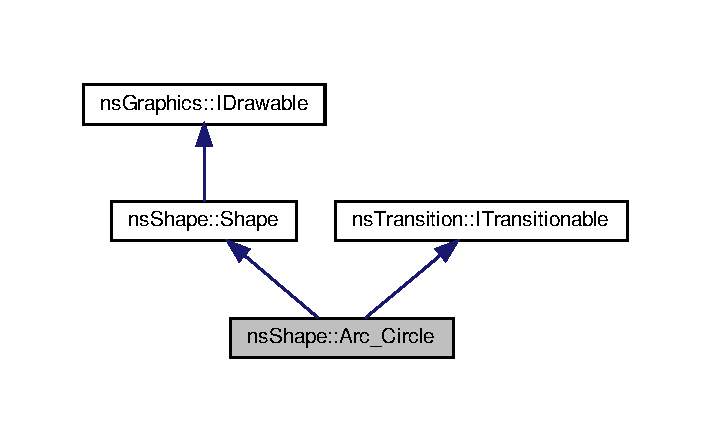
\includegraphics[width=341pt]{classns_shape_1_1_arc___circle__inherit__graph}
\end{center}
\end{figure}


Collaboration diagram for ns\+Shape\+:\+:Arc\+\_\+\+Circle\+:
\nopagebreak
\begin{figure}[H]
\begin{center}
\leavevmode
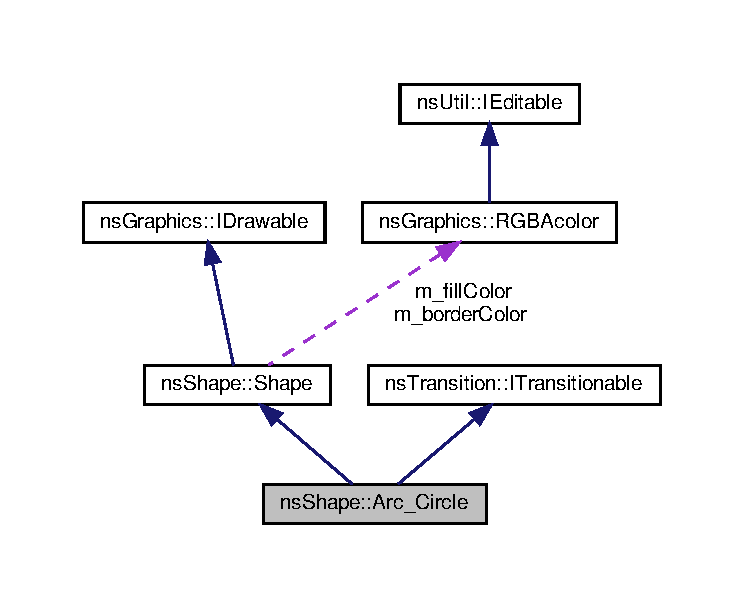
\includegraphics[width=350pt]{classns_shape_1_1_arc___circle__coll__graph}
\end{center}
\end{figure}
\subsection*{Public Types}
\begin{DoxyCompactItemize}
\item 
enum \hyperlink{classns_shape_1_1_arc___circle_aa6db8d435868af65e4ea134f37118415}{Transition\+Ids} \{ \newline
\hyperlink{classns_shape_1_1_arc___circle_aa6db8d435868af65e4ea134f37118415a86b008799c3b04b2ecc53c9093fe0ea8}{T\+R\+A\+N\+S\+I\+T\+I\+O\+N\+\_\+\+F\+I\+L\+L\+\_\+\+C\+O\+L\+O\+R\+\_\+\+R\+GB}, 
\hyperlink{classns_shape_1_1_arc___circle_aa6db8d435868af65e4ea134f37118415a519c50ae75ad4fc08870d40fc26f067a}{T\+R\+A\+N\+S\+I\+T\+I\+O\+N\+\_\+\+F\+I\+L\+L\+\_\+\+C\+O\+L\+O\+R\+\_\+\+A\+L\+P\+HA}, 
\hyperlink{classns_shape_1_1_arc___circle_aa6db8d435868af65e4ea134f37118415aadff30b38ed1e4ed7c407c9e632c4e87}{T\+R\+A\+N\+S\+I\+T\+I\+O\+N\+\_\+\+B\+O\+R\+D\+E\+R\+\_\+\+C\+O\+L\+O\+R\+\_\+\+R\+GB}, 
\hyperlink{classns_shape_1_1_arc___circle_aa6db8d435868af65e4ea134f37118415a000e5f7ac686f30aa86a276cd96a018b}{T\+R\+A\+N\+S\+I\+T\+I\+O\+N\+\_\+\+B\+O\+R\+D\+E\+R\+\_\+\+C\+O\+L\+O\+R\+\_\+\+A\+L\+P\+HA}, 
\newline
\hyperlink{classns_shape_1_1_arc___circle_aa6db8d435868af65e4ea134f37118415a8e5bcd350d6ffee20b2865f94695aa57}{T\+R\+A\+N\+S\+I\+T\+I\+O\+N\+\_\+\+P\+O\+S\+I\+T\+I\+ON}, 
\hyperlink{classns_shape_1_1_arc___circle_aa6db8d435868af65e4ea134f37118415a21d8c256199f323e30e7ad870c9cba50}{T\+R\+A\+N\+S\+I\+T\+I\+O\+N\+\_\+\+R\+A\+D\+I\+US}
 \}\begin{DoxyCompactList}\small\item\em Transition\+Ids \+: Liste de toutes les transitions que cet élément peut exécuter. \end{DoxyCompactList}
\end{DoxyCompactItemize}
\subsection*{Public Member Functions}
\begin{DoxyCompactItemize}
\item 
\hyperlink{classns_shape_1_1_arc___circle_a76dafed8fb69902ca33b784cce0a7975}{Arc\+\_\+\+Circle} (const \hyperlink{classns_graphics_1_1_vec2_d}{ns\+Graphics\+::\+Vec2D} \&position, const unsigned \&radius, const unsigned \&height, const char \&direction, const \hyperlink{classns_graphics_1_1_r_g_b_acolor}{ns\+Graphics\+::\+R\+G\+B\+Acolor} \&fill\+Color, const \hyperlink{classns_graphics_1_1_r_g_b_acolor}{ns\+Graphics\+::\+R\+G\+B\+Acolor} \&border\+Color=\hyperlink{namespacens_graphics_ab2001ad03cceb2565849e04465618c1e}{ns\+Graphics\+::\+K\+Transparent})
\begin{DoxyCompactList}\small\item\em Constructeur pour la classe \hyperlink{classns_shape_1_1_arc___circle}{Arc\+\_\+\+Circle}. \end{DoxyCompactList}\item 
virtual \hyperlink{classns_shape_1_1_arc___circle_a8b53fe0e24f1d0b1ad47331b8c66d289}{$\sim$\+Arc\+\_\+\+Circle} () override=default
\begin{DoxyCompactList}\small\item\em Destructeur virtuel pour la classe \hyperlink{classns_shape_1_1_arc___circle}{Arc\+\_\+\+Circle}. \end{DoxyCompactList}\item 
virtual void \hyperlink{classns_shape_1_1_arc___circle_a1e789ca962aeefd7dfd861eb0f75a6d7}{draw} (\hyperlink{class_min_g_l}{Min\+GL} \&window) const override
\begin{DoxyCompactList}\small\item\em Fonction pour afficher l\textquotesingle{}objet. \end{DoxyCompactList}\item 
virtual void \hyperlink{classns_shape_1_1_arc___circle_a11a5569112bf39b90192c7d7e0678736}{get\+Values} (const int \&id, std\+::vector$<$ float $>$ \&values) override
\begin{DoxyCompactList}\small\item\em Récupère des valeurs dans un vecteur de float pour l\textquotesingle{}ID spécifié \end{DoxyCompactList}\item 
virtual void \hyperlink{classns_shape_1_1_arc___circle_aa59b45d2a10ec5f8fd030d4ec46721b6}{set\+Values} (const int \&id, const std\+::vector$<$ float $>$ \&values) override
\begin{DoxyCompactList}\small\item\em Définit les nouvelles valeurs pour l\textquotesingle{}ID spécifié \end{DoxyCompactList}\item 
\hyperlink{classns_shape_1_1_arc___circle}{Arc\+\_\+\+Circle} \hyperlink{classns_shape_1_1_arc___circle_ac29fef537e801cbf80c148452772c770}{operator+} (const \hyperlink{classns_graphics_1_1_vec2_d}{ns\+Graphics\+::\+Vec2D} \&\hyperlink{classns_shape_1_1_arc___circle_a931e29f1d186676dd84e376dc6576254}{get\+Position}) const
\begin{DoxyCompactList}\small\item\em Opérateur de décalage. \end{DoxyCompactList}\item 
\hyperlink{classns_shape_1_1_arc___circle}{Arc\+\_\+\+Circle} \hyperlink{classns_shape_1_1_arc___circle_aa048e6ac6e09a351d78a2f9f6ebe0430}{operator$\ast$} (const float \&f) const
\begin{DoxyCompactList}\small\item\em Opérateur de réduction. \end{DoxyCompactList}\item 
const \hyperlink{classns_graphics_1_1_vec2_d}{ns\+Graphics\+::\+Vec2D} \& \hyperlink{classns_shape_1_1_arc___circle_a931e29f1d186676dd84e376dc6576254}{get\+Position} () const
\begin{DoxyCompactList}\small\item\em Récupère la position de l\textquotesingle{}arc de cercle. \end{DoxyCompactList}\item 
void \hyperlink{classns_shape_1_1_arc___circle_a52fa998838188e80ff97f96ad514cfe6}{set\+Position} (const \hyperlink{classns_graphics_1_1_vec2_d}{ns\+Graphics\+::\+Vec2D} \&position)
\begin{DoxyCompactList}\small\item\em Définit la nouvelle position de l\textquotesingle{}arc de cercle. \end{DoxyCompactList}\item 
unsigned \hyperlink{classns_shape_1_1_arc___circle_a7fbd0dc94a0a3de9fcb9352156e50d3b}{get\+Radius} () const
\begin{DoxyCompactList}\small\item\em Récupère le rayon de l\textquotesingle{}arc de cercle. \end{DoxyCompactList}\item 
void \hyperlink{classns_shape_1_1_arc___circle_ac0dac107441139a53881faa0be110eaa}{set\+Radius} (const unsigned \&radius)
\begin{DoxyCompactList}\small\item\em Définit le nouveau rayon de l\textquotesingle{}arc de cercle. \end{DoxyCompactList}\end{DoxyCompactItemize}
\subsection*{Additional Inherited Members}


\subsection{Detailed Description}
Classe représentant un arc de cercle. 

Definition at line 27 of file arc\+\_\+circle.\+h.



\subsection{Member Enumeration Documentation}
\mbox{\Hypertarget{classns_shape_1_1_arc___circle_aa6db8d435868af65e4ea134f37118415}\label{classns_shape_1_1_arc___circle_aa6db8d435868af65e4ea134f37118415}} 
\index{ns\+Shape\+::\+Arc\+\_\+\+Circle@{ns\+Shape\+::\+Arc\+\_\+\+Circle}!Transition\+Ids@{Transition\+Ids}}
\index{Transition\+Ids@{Transition\+Ids}!ns\+Shape\+::\+Arc\+\_\+\+Circle@{ns\+Shape\+::\+Arc\+\_\+\+Circle}}
\subsubsection{\texorpdfstring{Transition\+Ids}{TransitionIds}}
{\footnotesize\ttfamily enum \hyperlink{classns_shape_1_1_arc___circle_aa6db8d435868af65e4ea134f37118415}{ns\+Shape\+::\+Arc\+\_\+\+Circle\+::\+Transition\+Ids}}



Transition\+Ids \+: Liste de toutes les transitions que cet élément peut exécuter. 

\begin{DoxyEnumFields}{Enumerator}
\raisebox{\heightof{T}}[0pt][0pt]{\index{T\+R\+A\+N\+S\+I\+T\+I\+O\+N\+\_\+\+F\+I\+L\+L\+\_\+\+C\+O\+L\+O\+R\+\_\+\+R\+GB@{T\+R\+A\+N\+S\+I\+T\+I\+O\+N\+\_\+\+F\+I\+L\+L\+\_\+\+C\+O\+L\+O\+R\+\_\+\+R\+GB}!ns\+Shape\+::\+Arc\+\_\+\+Circle@{ns\+Shape\+::\+Arc\+\_\+\+Circle}}\index{ns\+Shape\+::\+Arc\+\_\+\+Circle@{ns\+Shape\+::\+Arc\+\_\+\+Circle}!T\+R\+A\+N\+S\+I\+T\+I\+O\+N\+\_\+\+F\+I\+L\+L\+\_\+\+C\+O\+L\+O\+R\+\_\+\+R\+GB@{T\+R\+A\+N\+S\+I\+T\+I\+O\+N\+\_\+\+F\+I\+L\+L\+\_\+\+C\+O\+L\+O\+R\+\_\+\+R\+GB}}}\mbox{\Hypertarget{classns_shape_1_1_arc___circle_aa6db8d435868af65e4ea134f37118415a86b008799c3b04b2ecc53c9093fe0ea8}\label{classns_shape_1_1_arc___circle_aa6db8d435868af65e4ea134f37118415a86b008799c3b04b2ecc53c9093fe0ea8}} 
T\+R\+A\+N\+S\+I\+T\+I\+O\+N\+\_\+\+F\+I\+L\+L\+\_\+\+C\+O\+L\+O\+R\+\_\+\+R\+GB&Transition pour la couleur de remplissage \\
\hline

\raisebox{\heightof{T}}[0pt][0pt]{\index{T\+R\+A\+N\+S\+I\+T\+I\+O\+N\+\_\+\+F\+I\+L\+L\+\_\+\+C\+O\+L\+O\+R\+\_\+\+A\+L\+P\+HA@{T\+R\+A\+N\+S\+I\+T\+I\+O\+N\+\_\+\+F\+I\+L\+L\+\_\+\+C\+O\+L\+O\+R\+\_\+\+A\+L\+P\+HA}!ns\+Shape\+::\+Arc\+\_\+\+Circle@{ns\+Shape\+::\+Arc\+\_\+\+Circle}}\index{ns\+Shape\+::\+Arc\+\_\+\+Circle@{ns\+Shape\+::\+Arc\+\_\+\+Circle}!T\+R\+A\+N\+S\+I\+T\+I\+O\+N\+\_\+\+F\+I\+L\+L\+\_\+\+C\+O\+L\+O\+R\+\_\+\+A\+L\+P\+HA@{T\+R\+A\+N\+S\+I\+T\+I\+O\+N\+\_\+\+F\+I\+L\+L\+\_\+\+C\+O\+L\+O\+R\+\_\+\+A\+L\+P\+HA}}}\mbox{\Hypertarget{classns_shape_1_1_arc___circle_aa6db8d435868af65e4ea134f37118415a519c50ae75ad4fc08870d40fc26f067a}\label{classns_shape_1_1_arc___circle_aa6db8d435868af65e4ea134f37118415a519c50ae75ad4fc08870d40fc26f067a}} 
T\+R\+A\+N\+S\+I\+T\+I\+O\+N\+\_\+\+F\+I\+L\+L\+\_\+\+C\+O\+L\+O\+R\+\_\+\+A\+L\+P\+HA&Transition pour la transparence de remplissage \\
\hline

\raisebox{\heightof{T}}[0pt][0pt]{\index{T\+R\+A\+N\+S\+I\+T\+I\+O\+N\+\_\+\+B\+O\+R\+D\+E\+R\+\_\+\+C\+O\+L\+O\+R\+\_\+\+R\+GB@{T\+R\+A\+N\+S\+I\+T\+I\+O\+N\+\_\+\+B\+O\+R\+D\+E\+R\+\_\+\+C\+O\+L\+O\+R\+\_\+\+R\+GB}!ns\+Shape\+::\+Arc\+\_\+\+Circle@{ns\+Shape\+::\+Arc\+\_\+\+Circle}}\index{ns\+Shape\+::\+Arc\+\_\+\+Circle@{ns\+Shape\+::\+Arc\+\_\+\+Circle}!T\+R\+A\+N\+S\+I\+T\+I\+O\+N\+\_\+\+B\+O\+R\+D\+E\+R\+\_\+\+C\+O\+L\+O\+R\+\_\+\+R\+GB@{T\+R\+A\+N\+S\+I\+T\+I\+O\+N\+\_\+\+B\+O\+R\+D\+E\+R\+\_\+\+C\+O\+L\+O\+R\+\_\+\+R\+GB}}}\mbox{\Hypertarget{classns_shape_1_1_arc___circle_aa6db8d435868af65e4ea134f37118415aadff30b38ed1e4ed7c407c9e632c4e87}\label{classns_shape_1_1_arc___circle_aa6db8d435868af65e4ea134f37118415aadff30b38ed1e4ed7c407c9e632c4e87}} 
T\+R\+A\+N\+S\+I\+T\+I\+O\+N\+\_\+\+B\+O\+R\+D\+E\+R\+\_\+\+C\+O\+L\+O\+R\+\_\+\+R\+GB&Transition pour la couleur de bord \\
\hline

\raisebox{\heightof{T}}[0pt][0pt]{\index{T\+R\+A\+N\+S\+I\+T\+I\+O\+N\+\_\+\+B\+O\+R\+D\+E\+R\+\_\+\+C\+O\+L\+O\+R\+\_\+\+A\+L\+P\+HA@{T\+R\+A\+N\+S\+I\+T\+I\+O\+N\+\_\+\+B\+O\+R\+D\+E\+R\+\_\+\+C\+O\+L\+O\+R\+\_\+\+A\+L\+P\+HA}!ns\+Shape\+::\+Arc\+\_\+\+Circle@{ns\+Shape\+::\+Arc\+\_\+\+Circle}}\index{ns\+Shape\+::\+Arc\+\_\+\+Circle@{ns\+Shape\+::\+Arc\+\_\+\+Circle}!T\+R\+A\+N\+S\+I\+T\+I\+O\+N\+\_\+\+B\+O\+R\+D\+E\+R\+\_\+\+C\+O\+L\+O\+R\+\_\+\+A\+L\+P\+HA@{T\+R\+A\+N\+S\+I\+T\+I\+O\+N\+\_\+\+B\+O\+R\+D\+E\+R\+\_\+\+C\+O\+L\+O\+R\+\_\+\+A\+L\+P\+HA}}}\mbox{\Hypertarget{classns_shape_1_1_arc___circle_aa6db8d435868af65e4ea134f37118415a000e5f7ac686f30aa86a276cd96a018b}\label{classns_shape_1_1_arc___circle_aa6db8d435868af65e4ea134f37118415a000e5f7ac686f30aa86a276cd96a018b}} 
T\+R\+A\+N\+S\+I\+T\+I\+O\+N\+\_\+\+B\+O\+R\+D\+E\+R\+\_\+\+C\+O\+L\+O\+R\+\_\+\+A\+L\+P\+HA&Transition pour la transparence de bord \\
\hline

\raisebox{\heightof{T}}[0pt][0pt]{\index{T\+R\+A\+N\+S\+I\+T\+I\+O\+N\+\_\+\+P\+O\+S\+I\+T\+I\+ON@{T\+R\+A\+N\+S\+I\+T\+I\+O\+N\+\_\+\+P\+O\+S\+I\+T\+I\+ON}!ns\+Shape\+::\+Arc\+\_\+\+Circle@{ns\+Shape\+::\+Arc\+\_\+\+Circle}}\index{ns\+Shape\+::\+Arc\+\_\+\+Circle@{ns\+Shape\+::\+Arc\+\_\+\+Circle}!T\+R\+A\+N\+S\+I\+T\+I\+O\+N\+\_\+\+P\+O\+S\+I\+T\+I\+ON@{T\+R\+A\+N\+S\+I\+T\+I\+O\+N\+\_\+\+P\+O\+S\+I\+T\+I\+ON}}}\mbox{\Hypertarget{classns_shape_1_1_arc___circle_aa6db8d435868af65e4ea134f37118415a8e5bcd350d6ffee20b2865f94695aa57}\label{classns_shape_1_1_arc___circle_aa6db8d435868af65e4ea134f37118415a8e5bcd350d6ffee20b2865f94695aa57}} 
T\+R\+A\+N\+S\+I\+T\+I\+O\+N\+\_\+\+P\+O\+S\+I\+T\+I\+ON&Transition pour la position \\
\hline

\raisebox{\heightof{T}}[0pt][0pt]{\index{T\+R\+A\+N\+S\+I\+T\+I\+O\+N\+\_\+\+R\+A\+D\+I\+US@{T\+R\+A\+N\+S\+I\+T\+I\+O\+N\+\_\+\+R\+A\+D\+I\+US}!ns\+Shape\+::\+Arc\+\_\+\+Circle@{ns\+Shape\+::\+Arc\+\_\+\+Circle}}\index{ns\+Shape\+::\+Arc\+\_\+\+Circle@{ns\+Shape\+::\+Arc\+\_\+\+Circle}!T\+R\+A\+N\+S\+I\+T\+I\+O\+N\+\_\+\+R\+A\+D\+I\+US@{T\+R\+A\+N\+S\+I\+T\+I\+O\+N\+\_\+\+R\+A\+D\+I\+US}}}\mbox{\Hypertarget{classns_shape_1_1_arc___circle_aa6db8d435868af65e4ea134f37118415a21d8c256199f323e30e7ad870c9cba50}\label{classns_shape_1_1_arc___circle_aa6db8d435868af65e4ea134f37118415a21d8c256199f323e30e7ad870c9cba50}} 
T\+R\+A\+N\+S\+I\+T\+I\+O\+N\+\_\+\+R\+A\+D\+I\+US&Transition pour le rayon \\
\hline

\end{DoxyEnumFields}


Definition at line 34 of file arc\+\_\+circle.\+h.



\subsection{Constructor \& Destructor Documentation}
\mbox{\Hypertarget{classns_shape_1_1_arc___circle_a76dafed8fb69902ca33b784cce0a7975}\label{classns_shape_1_1_arc___circle_a76dafed8fb69902ca33b784cce0a7975}} 
\index{ns\+Shape\+::\+Arc\+\_\+\+Circle@{ns\+Shape\+::\+Arc\+\_\+\+Circle}!Arc\+\_\+\+Circle@{Arc\+\_\+\+Circle}}
\index{Arc\+\_\+\+Circle@{Arc\+\_\+\+Circle}!ns\+Shape\+::\+Arc\+\_\+\+Circle@{ns\+Shape\+::\+Arc\+\_\+\+Circle}}
\subsubsection{\texorpdfstring{Arc\+\_\+\+Circle()}{Arc\_Circle()}}
{\footnotesize\ttfamily ns\+Shape\+::\+Arc\+\_\+\+Circle\+::\+Arc\+\_\+\+Circle (\begin{DoxyParamCaption}\item[{const \hyperlink{classns_graphics_1_1_vec2_d}{ns\+Graphics\+::\+Vec2D} \&}]{position,  }\item[{const unsigned \&}]{radius,  }\item[{const unsigned \&}]{height,  }\item[{const char \&}]{direction,  }\item[{const \hyperlink{classns_graphics_1_1_r_g_b_acolor}{ns\+Graphics\+::\+R\+G\+B\+Acolor} \&}]{fill\+Color,  }\item[{const \hyperlink{classns_graphics_1_1_r_g_b_acolor}{ns\+Graphics\+::\+R\+G\+B\+Acolor} \&}]{border\+Color = {\ttfamily \hyperlink{namespacens_graphics_ab2001ad03cceb2565849e04465618c1e}{ns\+Graphics\+::\+K\+Transparent}} }\end{DoxyParamCaption})}



Constructeur pour la classe \hyperlink{classns_shape_1_1_arc___circle}{Arc\+\_\+\+Circle}. 


\begin{DoxyParams}[1]{Parameters}
\mbox{\tt in}  & {\em first\+Position} & \+: Position du centre \\
\hline
\mbox{\tt in}  & {\em radius} & \+: Rayon de l\textquotesingle{}arc de cercle \\
\hline
\mbox{\tt in}  & {\em height} & \+: Hauteur de l\textquotesingle{}arc de cercle \\
\hline
\mbox{\tt in}  & {\em direction} & \+: Direction de l\textquotesingle{}arc de cercle \\
\hline
\mbox{\tt in}  & {\em fill\+Color} & \+: Couleur de remplissage \\
\hline
\mbox{\tt in}  & {\em border\+Color} & \+: Couleur de bord \\
\hline
\end{DoxyParams}


Definition at line 13 of file arc\+\_\+circle.\+cpp.

\mbox{\Hypertarget{classns_shape_1_1_arc___circle_a8b53fe0e24f1d0b1ad47331b8c66d289}\label{classns_shape_1_1_arc___circle_a8b53fe0e24f1d0b1ad47331b8c66d289}} 
\index{ns\+Shape\+::\+Arc\+\_\+\+Circle@{ns\+Shape\+::\+Arc\+\_\+\+Circle}!````~Arc\+\_\+\+Circle@{$\sim$\+Arc\+\_\+\+Circle}}
\index{````~Arc\+\_\+\+Circle@{$\sim$\+Arc\+\_\+\+Circle}!ns\+Shape\+::\+Arc\+\_\+\+Circle@{ns\+Shape\+::\+Arc\+\_\+\+Circle}}
\subsubsection{\texorpdfstring{$\sim$\+Arc\+\_\+\+Circle()}{~Arc\_Circle()}}
{\footnotesize\ttfamily ns\+Shape\+::\+Arc\+\_\+\+Circle\+::$\sim$\+Arc\+\_\+\+Circle (\begin{DoxyParamCaption}{ }\end{DoxyParamCaption})\hspace{0.3cm}{\ttfamily [override]}, {\ttfamily [virtual]}, {\ttfamily [default]}}



Destructeur virtuel pour la classe \hyperlink{classns_shape_1_1_arc___circle}{Arc\+\_\+\+Circle}. 



\subsection{Member Function Documentation}
\mbox{\Hypertarget{classns_shape_1_1_arc___circle_a1e789ca962aeefd7dfd861eb0f75a6d7}\label{classns_shape_1_1_arc___circle_a1e789ca962aeefd7dfd861eb0f75a6d7}} 
\index{ns\+Shape\+::\+Arc\+\_\+\+Circle@{ns\+Shape\+::\+Arc\+\_\+\+Circle}!draw@{draw}}
\index{draw@{draw}!ns\+Shape\+::\+Arc\+\_\+\+Circle@{ns\+Shape\+::\+Arc\+\_\+\+Circle}}
\subsubsection{\texorpdfstring{draw()}{draw()}}
{\footnotesize\ttfamily void ns\+Shape\+::\+Arc\+\_\+\+Circle\+::draw (\begin{DoxyParamCaption}\item[{\hyperlink{class_min_g_l}{Min\+GL} \&}]{window }\end{DoxyParamCaption}) const\hspace{0.3cm}{\ttfamily [override]}, {\ttfamily [virtual]}}



Fonction pour afficher l\textquotesingle{}objet. 



Implements \hyperlink{classns_graphics_1_1_i_drawable_abed8a61e1d507d31e76f0891f3bf9c51}{ns\+Graphics\+::\+I\+Drawable}.



Definition at line 21 of file arc\+\_\+circle.\+cpp.

\mbox{\Hypertarget{classns_shape_1_1_arc___circle_a931e29f1d186676dd84e376dc6576254}\label{classns_shape_1_1_arc___circle_a931e29f1d186676dd84e376dc6576254}} 
\index{ns\+Shape\+::\+Arc\+\_\+\+Circle@{ns\+Shape\+::\+Arc\+\_\+\+Circle}!get\+Position@{get\+Position}}
\index{get\+Position@{get\+Position}!ns\+Shape\+::\+Arc\+\_\+\+Circle@{ns\+Shape\+::\+Arc\+\_\+\+Circle}}
\subsubsection{\texorpdfstring{get\+Position()}{getPosition()}}
{\footnotesize\ttfamily const \hyperlink{classns_graphics_1_1_vec2_d}{ns\+Graphics\+::\+Vec2D} \& ns\+Shape\+::\+Arc\+\_\+\+Circle\+::get\+Position (\begin{DoxyParamCaption}{ }\end{DoxyParamCaption}) const}



Récupère la position de l\textquotesingle{}arc de cercle. 

\mbox{\Hypertarget{classns_shape_1_1_arc___circle_a7fbd0dc94a0a3de9fcb9352156e50d3b}\label{classns_shape_1_1_arc___circle_a7fbd0dc94a0a3de9fcb9352156e50d3b}} 
\index{ns\+Shape\+::\+Arc\+\_\+\+Circle@{ns\+Shape\+::\+Arc\+\_\+\+Circle}!get\+Radius@{get\+Radius}}
\index{get\+Radius@{get\+Radius}!ns\+Shape\+::\+Arc\+\_\+\+Circle@{ns\+Shape\+::\+Arc\+\_\+\+Circle}}
\subsubsection{\texorpdfstring{get\+Radius()}{getRadius()}}
{\footnotesize\ttfamily unsigned ns\+Shape\+::\+Arc\+\_\+\+Circle\+::get\+Radius (\begin{DoxyParamCaption}{ }\end{DoxyParamCaption}) const}



Récupère le rayon de l\textquotesingle{}arc de cercle. 

\mbox{\Hypertarget{classns_shape_1_1_arc___circle_a11a5569112bf39b90192c7d7e0678736}\label{classns_shape_1_1_arc___circle_a11a5569112bf39b90192c7d7e0678736}} 
\index{ns\+Shape\+::\+Arc\+\_\+\+Circle@{ns\+Shape\+::\+Arc\+\_\+\+Circle}!get\+Values@{get\+Values}}
\index{get\+Values@{get\+Values}!ns\+Shape\+::\+Arc\+\_\+\+Circle@{ns\+Shape\+::\+Arc\+\_\+\+Circle}}
\subsubsection{\texorpdfstring{get\+Values()}{getValues()}}
{\footnotesize\ttfamily void ns\+Shape\+::\+Arc\+\_\+\+Circle\+::get\+Values (\begin{DoxyParamCaption}\item[{const int \&}]{id,  }\item[{std\+::vector$<$ float $>$ \&}]{values }\end{DoxyParamCaption})\hspace{0.3cm}{\ttfamily [override]}, {\ttfamily [virtual]}}



Récupère des valeurs dans un vecteur de float pour l\textquotesingle{}ID spécifié 


\begin{DoxyParams}[1]{Parameters}
\mbox{\tt in}  & {\em id} & ID des valeurs a récupérer \\
\hline
\mbox{\tt in,out}  & {\em values} & Vecteur de valeurs a peupler \\
\hline
\end{DoxyParams}


Implements \hyperlink{classns_transition_1_1_i_transitionable_a5871a16fd47c1e5c8bacdd5da8597ed9}{ns\+Transition\+::\+I\+Transitionable}.



Definition at line 56 of file arc\+\_\+circle.\+cpp.

\mbox{\Hypertarget{classns_shape_1_1_arc___circle_aa048e6ac6e09a351d78a2f9f6ebe0430}\label{classns_shape_1_1_arc___circle_aa048e6ac6e09a351d78a2f9f6ebe0430}} 
\index{ns\+Shape\+::\+Arc\+\_\+\+Circle@{ns\+Shape\+::\+Arc\+\_\+\+Circle}!operator$\ast$@{operator$\ast$}}
\index{operator$\ast$@{operator$\ast$}!ns\+Shape\+::\+Arc\+\_\+\+Circle@{ns\+Shape\+::\+Arc\+\_\+\+Circle}}
\subsubsection{\texorpdfstring{operator$\ast$()}{operator*()}}
{\footnotesize\ttfamily \hyperlink{classns_shape_1_1_arc___circle}{Arc\+\_\+\+Circle} ns\+Shape\+::\+Arc\+\_\+\+Circle\+::operator$\ast$ (\begin{DoxyParamCaption}\item[{const float \&}]{f }\end{DoxyParamCaption}) const}



Opérateur de réduction. 


\begin{DoxyParams}[1]{Parameters}
\mbox{\tt in}  & {\em f} & \+: Nombre avec lequel multiplier la position actuelle \\
\hline
\end{DoxyParams}
\mbox{\Hypertarget{classns_shape_1_1_arc___circle_ac29fef537e801cbf80c148452772c770}\label{classns_shape_1_1_arc___circle_ac29fef537e801cbf80c148452772c770}} 
\index{ns\+Shape\+::\+Arc\+\_\+\+Circle@{ns\+Shape\+::\+Arc\+\_\+\+Circle}!operator+@{operator+}}
\index{operator+@{operator+}!ns\+Shape\+::\+Arc\+\_\+\+Circle@{ns\+Shape\+::\+Arc\+\_\+\+Circle}}
\subsubsection{\texorpdfstring{operator+()}{operator+()}}
{\footnotesize\ttfamily \hyperlink{classns_shape_1_1_arc___circle}{Arc\+\_\+\+Circle} ns\+Shape\+::\+Arc\+\_\+\+Circle\+::operator+ (\begin{DoxyParamCaption}\item[{const \hyperlink{classns_graphics_1_1_vec2_d}{ns\+Graphics\+::\+Vec2D} \&}]{position }\end{DoxyParamCaption}) const}



Opérateur de décalage. 


\begin{DoxyParams}[1]{Parameters}
\mbox{\tt in}  & {\em position} & \+: Position a additionner \\
\hline
\end{DoxyParams}
\mbox{\Hypertarget{classns_shape_1_1_arc___circle_a52fa998838188e80ff97f96ad514cfe6}\label{classns_shape_1_1_arc___circle_a52fa998838188e80ff97f96ad514cfe6}} 
\index{ns\+Shape\+::\+Arc\+\_\+\+Circle@{ns\+Shape\+::\+Arc\+\_\+\+Circle}!set\+Position@{set\+Position}}
\index{set\+Position@{set\+Position}!ns\+Shape\+::\+Arc\+\_\+\+Circle@{ns\+Shape\+::\+Arc\+\_\+\+Circle}}
\subsubsection{\texorpdfstring{set\+Position()}{setPosition()}}
{\footnotesize\ttfamily ns\+Shape\+::\+Arc\+\_\+\+Circle\+::set\+Position (\begin{DoxyParamCaption}\item[{const \hyperlink{classns_graphics_1_1_vec2_d}{ns\+Graphics\+::\+Vec2D} \&}]{position }\end{DoxyParamCaption})}



Définit la nouvelle position de l\textquotesingle{}arc de cercle. 


\begin{DoxyParams}[1]{Parameters}
\mbox{\tt in}  & {\em position} & \+: Nouvelle position \\
\hline
\end{DoxyParams}
\mbox{\Hypertarget{classns_shape_1_1_arc___circle_ac0dac107441139a53881faa0be110eaa}\label{classns_shape_1_1_arc___circle_ac0dac107441139a53881faa0be110eaa}} 
\index{ns\+Shape\+::\+Arc\+\_\+\+Circle@{ns\+Shape\+::\+Arc\+\_\+\+Circle}!set\+Radius@{set\+Radius}}
\index{set\+Radius@{set\+Radius}!ns\+Shape\+::\+Arc\+\_\+\+Circle@{ns\+Shape\+::\+Arc\+\_\+\+Circle}}
\subsubsection{\texorpdfstring{set\+Radius()}{setRadius()}}
{\footnotesize\ttfamily ns\+Shape\+::\+Arc\+\_\+\+Circle\+::set\+Radius (\begin{DoxyParamCaption}\item[{const unsigned \&}]{radius }\end{DoxyParamCaption})}



Définit le nouveau rayon de l\textquotesingle{}arc de cercle. 


\begin{DoxyParams}[1]{Parameters}
\mbox{\tt in}  & {\em radius} & \+: Nouveau rayon \\
\hline
\end{DoxyParams}
\mbox{\Hypertarget{classns_shape_1_1_arc___circle_aa59b45d2a10ec5f8fd030d4ec46721b6}\label{classns_shape_1_1_arc___circle_aa59b45d2a10ec5f8fd030d4ec46721b6}} 
\index{ns\+Shape\+::\+Arc\+\_\+\+Circle@{ns\+Shape\+::\+Arc\+\_\+\+Circle}!set\+Values@{set\+Values}}
\index{set\+Values@{set\+Values}!ns\+Shape\+::\+Arc\+\_\+\+Circle@{ns\+Shape\+::\+Arc\+\_\+\+Circle}}
\subsubsection{\texorpdfstring{set\+Values()}{setValues()}}
{\footnotesize\ttfamily void ns\+Shape\+::\+Arc\+\_\+\+Circle\+::set\+Values (\begin{DoxyParamCaption}\item[{const int \&}]{id,  }\item[{const std\+::vector$<$ float $>$ \&}]{values }\end{DoxyParamCaption})\hspace{0.3cm}{\ttfamily [override]}, {\ttfamily [virtual]}}



Définit les nouvelles valeurs pour l\textquotesingle{}ID spécifié 


\begin{DoxyParams}[1]{Parameters}
\mbox{\tt in}  & {\em id} & ID des valeurs a définir \\
\hline
\mbox{\tt in}  & {\em values} & Vecteur des nouvelles valeurs a appliquer \\
\hline
\end{DoxyParams}


Implements \hyperlink{classns_transition_1_1_i_transitionable_ade37d29f7f2ca4890ed0e2e64d033197}{ns\+Transition\+::\+I\+Transitionable}.



Definition at line 96 of file arc\+\_\+circle.\+cpp.



The documentation for this class was generated from the following files\+:\begin{DoxyCompactItemize}
\item 
libs/game/graphic/\hyperlink{arc__circle_8h}{arc\+\_\+circle.\+h}\item 
src/graphic/\hyperlink{arc__circle_8cpp}{arc\+\_\+circle.\+cpp}\end{DoxyCompactItemize}

\hypertarget{classns_audio_1_1_audio_engine}{}\section{ns\+Audio\+:\+:Audio\+Engine Class Reference}
\label{classns_audio_1_1_audio_engine}\index{ns\+Audio\+::\+Audio\+Engine@{ns\+Audio\+::\+Audio\+Engine}}


Une classe de gestion des effets audio et de la musique.  




{\ttfamily \#include $<$audioengine.\+h$>$}

\subsection*{Public Member Functions}
\begin{DoxyCompactItemize}
\item 
void \hyperlink{classns_audio_1_1_audio_engine_a6ef72eb80bef2c1b0764c40f629d2536}{set\+Music} (const std\+::string \&file\+Name, bool loop=true)
\begin{DoxyCompactList}\small\item\em Définit le fichier audio de la musique. \end{DoxyCompactList}\item 
void \hyperlink{classns_audio_1_1_audio_engine_aba89263fc9f810bee40dcae229313883}{toggle\+Music\+Playing} ()
\begin{DoxyCompactList}\small\item\em Met en pause ou relance la musique. \end{DoxyCompactList}\item 
void \hyperlink{classns_audio_1_1_audio_engine_ac21b2c1be9590a0f702c48220c59f8c9}{set\+Music\+Playing} (bool playing)
\begin{DoxyCompactList}\small\item\em Règle l\textquotesingle{}état de lecture de la musique. \end{DoxyCompactList}\item 
bool \hyperlink{classns_audio_1_1_audio_engine_a57e13380a3039e546a5f1b9242f8709b}{is\+Music\+Playing} () const
\begin{DoxyCompactList}\small\item\em Récupère l\textquotesingle{}état de lecture de la musique. \end{DoxyCompactList}\item 
void \hyperlink{classns_audio_1_1_audio_engine_a4c88595136327b3805c0322a9a8d2a0f}{load\+Sound} (const std\+::string \&file\+Name)
\begin{DoxyCompactList}\small\item\em Charge un fichier audio dans un buffer. \end{DoxyCompactList}\item 
void \hyperlink{classns_audio_1_1_audio_engine_a2b0a1a9b1cb90e1180ddedb5b9e2fad1}{remove\+Buffer} (const std\+::string \&file\+Name)
\begin{DoxyCompactList}\small\item\em Retire un buffer de la liste. \end{DoxyCompactList}\item 
void \hyperlink{classns_audio_1_1_audio_engine_ac05b3e0d2fd9ecfd1ad8eb110f021bf3}{empty\+Buffer\+List} ()
\begin{DoxyCompactList}\small\item\em Vide la liste des buffers. \end{DoxyCompactList}\item 
void \hyperlink{classns_audio_1_1_audio_engine_ac1343ed3afe38eb80a222969f3d74d6d}{start\+Music\+From\+Beginning} ()
\begin{DoxyCompactList}\small\item\em Relance la musique depuis le début. \end{DoxyCompactList}\item 
void \hyperlink{classns_audio_1_1_audio_engine_a47d769cc331578a398f422ff497505c8}{play\+Sound\+From\+Buffer} (const std\+::string \&file\+Name)
\begin{DoxyCompactList}\small\item\em Joue un son depuis un buffer. \end{DoxyCompactList}\item 
void \hyperlink{classns_audio_1_1_audio_engine_aa541e8088c35ab41e4747ecd648e75e9}{play\+Sound\+From\+File} (const std\+::string \&file\+Name)
\begin{DoxyCompactList}\small\item\em Joue un son depuis un fichier. \end{DoxyCompactList}\end{DoxyCompactItemize}


\subsection{Detailed Description}
Une classe de gestion des effets audio et de la musique. 

Definition at line 28 of file audioengine.\+h.



\subsection{Member Function Documentation}
\mbox{\Hypertarget{classns_audio_1_1_audio_engine_ac05b3e0d2fd9ecfd1ad8eb110f021bf3}\label{classns_audio_1_1_audio_engine_ac05b3e0d2fd9ecfd1ad8eb110f021bf3}} 
\index{ns\+Audio\+::\+Audio\+Engine@{ns\+Audio\+::\+Audio\+Engine}!empty\+Buffer\+List@{empty\+Buffer\+List}}
\index{empty\+Buffer\+List@{empty\+Buffer\+List}!ns\+Audio\+::\+Audio\+Engine@{ns\+Audio\+::\+Audio\+Engine}}
\subsubsection{\texorpdfstring{empty\+Buffer\+List()}{emptyBufferList()}}
{\footnotesize\ttfamily void ns\+Audio\+::\+Audio\+Engine\+::empty\+Buffer\+List (\begin{DoxyParamCaption}{ }\end{DoxyParamCaption})}



Vide la liste des buffers. 

\mbox{\Hypertarget{classns_audio_1_1_audio_engine_a57e13380a3039e546a5f1b9242f8709b}\label{classns_audio_1_1_audio_engine_a57e13380a3039e546a5f1b9242f8709b}} 
\index{ns\+Audio\+::\+Audio\+Engine@{ns\+Audio\+::\+Audio\+Engine}!is\+Music\+Playing@{is\+Music\+Playing}}
\index{is\+Music\+Playing@{is\+Music\+Playing}!ns\+Audio\+::\+Audio\+Engine@{ns\+Audio\+::\+Audio\+Engine}}
\subsubsection{\texorpdfstring{is\+Music\+Playing()}{isMusicPlaying()}}
{\footnotesize\ttfamily bool ns\+Audio\+::\+Audio\+Engine\+::is\+Music\+Playing (\begin{DoxyParamCaption}{ }\end{DoxyParamCaption}) const}



Récupère l\textquotesingle{}état de lecture de la musique. 

\mbox{\Hypertarget{classns_audio_1_1_audio_engine_a4c88595136327b3805c0322a9a8d2a0f}\label{classns_audio_1_1_audio_engine_a4c88595136327b3805c0322a9a8d2a0f}} 
\index{ns\+Audio\+::\+Audio\+Engine@{ns\+Audio\+::\+Audio\+Engine}!load\+Sound@{load\+Sound}}
\index{load\+Sound@{load\+Sound}!ns\+Audio\+::\+Audio\+Engine@{ns\+Audio\+::\+Audio\+Engine}}
\subsubsection{\texorpdfstring{load\+Sound()}{loadSound()}}
{\footnotesize\ttfamily void ns\+Audio\+::\+Audio\+Engine\+::load\+Sound (\begin{DoxyParamCaption}\item[{const std\+::string \&}]{file\+Name }\end{DoxyParamCaption})}



Charge un fichier audio dans un buffer. 

\mbox{\Hypertarget{classns_audio_1_1_audio_engine_a47d769cc331578a398f422ff497505c8}\label{classns_audio_1_1_audio_engine_a47d769cc331578a398f422ff497505c8}} 
\index{ns\+Audio\+::\+Audio\+Engine@{ns\+Audio\+::\+Audio\+Engine}!play\+Sound\+From\+Buffer@{play\+Sound\+From\+Buffer}}
\index{play\+Sound\+From\+Buffer@{play\+Sound\+From\+Buffer}!ns\+Audio\+::\+Audio\+Engine@{ns\+Audio\+::\+Audio\+Engine}}
\subsubsection{\texorpdfstring{play\+Sound\+From\+Buffer()}{playSoundFromBuffer()}}
{\footnotesize\ttfamily void ns\+Audio\+::\+Audio\+Engine\+::play\+Sound\+From\+Buffer (\begin{DoxyParamCaption}\item[{const std\+::string \&}]{file\+Name }\end{DoxyParamCaption})}



Joue un son depuis un buffer. 


\begin{DoxyParams}[1]{Parameters}
\mbox{\tt in}  & {\em file\+Name} & \+: nom du fichier \\
\hline
\end{DoxyParams}
\mbox{\Hypertarget{classns_audio_1_1_audio_engine_aa541e8088c35ab41e4747ecd648e75e9}\label{classns_audio_1_1_audio_engine_aa541e8088c35ab41e4747ecd648e75e9}} 
\index{ns\+Audio\+::\+Audio\+Engine@{ns\+Audio\+::\+Audio\+Engine}!play\+Sound\+From\+File@{play\+Sound\+From\+File}}
\index{play\+Sound\+From\+File@{play\+Sound\+From\+File}!ns\+Audio\+::\+Audio\+Engine@{ns\+Audio\+::\+Audio\+Engine}}
\subsubsection{\texorpdfstring{play\+Sound\+From\+File()}{playSoundFromFile()}}
{\footnotesize\ttfamily void ns\+Audio\+::\+Audio\+Engine\+::play\+Sound\+From\+File (\begin{DoxyParamCaption}\item[{const std\+::string \&}]{file\+Name }\end{DoxyParamCaption})}



Joue un son depuis un fichier. 


\begin{DoxyParams}[1]{Parameters}
\mbox{\tt in}  & {\em file\+Name} & \+: nom du fichier \\
\hline
\end{DoxyParams}
\mbox{\Hypertarget{classns_audio_1_1_audio_engine_a2b0a1a9b1cb90e1180ddedb5b9e2fad1}\label{classns_audio_1_1_audio_engine_a2b0a1a9b1cb90e1180ddedb5b9e2fad1}} 
\index{ns\+Audio\+::\+Audio\+Engine@{ns\+Audio\+::\+Audio\+Engine}!remove\+Buffer@{remove\+Buffer}}
\index{remove\+Buffer@{remove\+Buffer}!ns\+Audio\+::\+Audio\+Engine@{ns\+Audio\+::\+Audio\+Engine}}
\subsubsection{\texorpdfstring{remove\+Buffer()}{removeBuffer()}}
{\footnotesize\ttfamily void ns\+Audio\+::\+Audio\+Engine\+::remove\+Buffer (\begin{DoxyParamCaption}\item[{const std\+::string \&}]{file\+Name }\end{DoxyParamCaption})}



Retire un buffer de la liste. 

\mbox{\Hypertarget{classns_audio_1_1_audio_engine_a6ef72eb80bef2c1b0764c40f629d2536}\label{classns_audio_1_1_audio_engine_a6ef72eb80bef2c1b0764c40f629d2536}} 
\index{ns\+Audio\+::\+Audio\+Engine@{ns\+Audio\+::\+Audio\+Engine}!set\+Music@{set\+Music}}
\index{set\+Music@{set\+Music}!ns\+Audio\+::\+Audio\+Engine@{ns\+Audio\+::\+Audio\+Engine}}
\subsubsection{\texorpdfstring{set\+Music()}{setMusic()}}
{\footnotesize\ttfamily void ns\+Audio\+::\+Audio\+Engine\+::set\+Music (\begin{DoxyParamCaption}\item[{const std\+::string \&}]{file\+Name,  }\item[{bool}]{loop = {\ttfamily true} }\end{DoxyParamCaption})}



Définit le fichier audio de la musique. 


\begin{DoxyParams}[1]{Parameters}
\mbox{\tt in}  & {\em file\+Name} & \+: nom du fichier \\
\hline
\mbox{\tt in}  & {\em loop} & \+: indique si la musique est lue en boucle ou non (oui par défaut) \\
\hline
\end{DoxyParams}
\mbox{\Hypertarget{classns_audio_1_1_audio_engine_ac21b2c1be9590a0f702c48220c59f8c9}\label{classns_audio_1_1_audio_engine_ac21b2c1be9590a0f702c48220c59f8c9}} 
\index{ns\+Audio\+::\+Audio\+Engine@{ns\+Audio\+::\+Audio\+Engine}!set\+Music\+Playing@{set\+Music\+Playing}}
\index{set\+Music\+Playing@{set\+Music\+Playing}!ns\+Audio\+::\+Audio\+Engine@{ns\+Audio\+::\+Audio\+Engine}}
\subsubsection{\texorpdfstring{set\+Music\+Playing()}{setMusicPlaying()}}
{\footnotesize\ttfamily void ns\+Audio\+::\+Audio\+Engine\+::set\+Music\+Playing (\begin{DoxyParamCaption}\item[{bool}]{playing }\end{DoxyParamCaption})}



Règle l\textquotesingle{}état de lecture de la musique. 


\begin{DoxyParams}[1]{Parameters}
\mbox{\tt in}  & {\em playing} & \+: Nouvel état de lecture \\
\hline
\end{DoxyParams}
\mbox{\Hypertarget{classns_audio_1_1_audio_engine_ac1343ed3afe38eb80a222969f3d74d6d}\label{classns_audio_1_1_audio_engine_ac1343ed3afe38eb80a222969f3d74d6d}} 
\index{ns\+Audio\+::\+Audio\+Engine@{ns\+Audio\+::\+Audio\+Engine}!start\+Music\+From\+Beginning@{start\+Music\+From\+Beginning}}
\index{start\+Music\+From\+Beginning@{start\+Music\+From\+Beginning}!ns\+Audio\+::\+Audio\+Engine@{ns\+Audio\+::\+Audio\+Engine}}
\subsubsection{\texorpdfstring{start\+Music\+From\+Beginning()}{startMusicFromBeginning()}}
{\footnotesize\ttfamily void ns\+Audio\+::\+Audio\+Engine\+::start\+Music\+From\+Beginning (\begin{DoxyParamCaption}{ }\end{DoxyParamCaption})}



Relance la musique depuis le début. 

\mbox{\Hypertarget{classns_audio_1_1_audio_engine_aba89263fc9f810bee40dcae229313883}\label{classns_audio_1_1_audio_engine_aba89263fc9f810bee40dcae229313883}} 
\index{ns\+Audio\+::\+Audio\+Engine@{ns\+Audio\+::\+Audio\+Engine}!toggle\+Music\+Playing@{toggle\+Music\+Playing}}
\index{toggle\+Music\+Playing@{toggle\+Music\+Playing}!ns\+Audio\+::\+Audio\+Engine@{ns\+Audio\+::\+Audio\+Engine}}
\subsubsection{\texorpdfstring{toggle\+Music\+Playing()}{toggleMusicPlaying()}}
{\footnotesize\ttfamily void ns\+Audio\+::\+Audio\+Engine\+::toggle\+Music\+Playing (\begin{DoxyParamCaption}{ }\end{DoxyParamCaption})}



Met en pause ou relance la musique. 



The documentation for this class was generated from the following file\+:\begin{DoxyCompactItemize}
\item 
libs/mingl/audio/\hyperlink{audioengine_8h}{audioengine.\+h}\end{DoxyCompactItemize}

\hypertarget{classns_exception_1_1_c_exception}{}\section{ns\+Exception\+:\+:C\+Exception Class Reference}
\label{classns_exception_1_1_c_exception}\index{ns\+Exception\+::\+C\+Exception@{ns\+Exception\+::\+C\+Exception}}


Classe pour créer des exceptions facilement.  




{\ttfamily \#include $<$cexception.\+h$>$}



Inheritance diagram for ns\+Exception\+:\+:C\+Exception\+:
\nopagebreak
\begin{figure}[H]
\begin{center}
\leavevmode
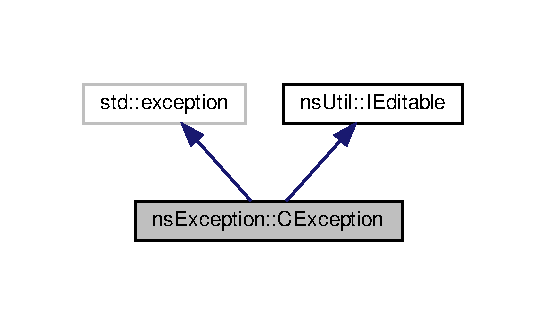
\includegraphics[width=262pt]{classns_exception_1_1_c_exception__inherit__graph}
\end{center}
\end{figure}


Collaboration diagram for ns\+Exception\+:\+:C\+Exception\+:
\nopagebreak
\begin{figure}[H]
\begin{center}
\leavevmode
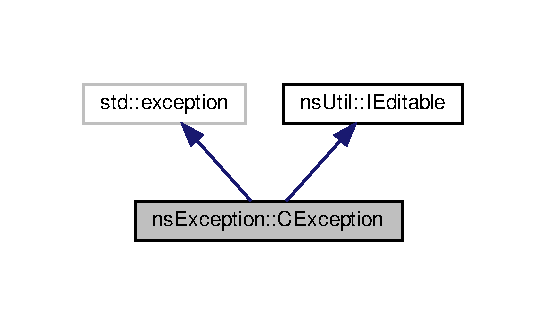
\includegraphics[width=262pt]{classns_exception_1_1_c_exception__coll__graph}
\end{center}
\end{figure}
\subsection*{Public Member Functions}
\begin{DoxyCompactItemize}
\item 
\hyperlink{classns_exception_1_1_c_exception_aeacba2e2180dd8c00c643e1a67cba423}{C\+Exception} (const std\+::string \&Libelle=std\+::string(), const unsigned Cod\+Err=\hyperlink{namespacens_exception_ae4cd0d6bbd5590a1b121347632d41376a0446a2a6f75ad46276a3c6bfbcf06eb3}{K\+No\+Exc})
\begin{DoxyCompactList}\small\item\em Constructeur pour la classe \hyperlink{classns_exception_1_1_c_exception}{C\+Exception}. \end{DoxyCompactList}\item 
virtual \hyperlink{classns_exception_1_1_c_exception_a8b95a8f59d50a7ff3b67423c83cb8501}{$\sim$\+C\+Exception} () override=default
\begin{DoxyCompactList}\small\item\em Destructeur virtuel pour la classe \hyperlink{classns_exception_1_1_c_exception}{C\+Exception}. \end{DoxyCompactList}\item 
const std\+::string \& \hyperlink{classns_exception_1_1_c_exception_aef8e3d1a4e22ec7045d7d0b14d8b968a}{Get\+Libelle} () const
\begin{DoxyCompactList}\small\item\em Récupère le libellé de l\textquotesingle{}exception. \end{DoxyCompactList}\item 
unsigned \hyperlink{classns_exception_1_1_c_exception_adf06d1598420c7b60c1b134bf2a946c2}{Get\+Cod\+Err} () const
\begin{DoxyCompactList}\small\item\em Récupère le code erreur de l\textquotesingle{}exception. \end{DoxyCompactList}\item 
virtual const char $\ast$ \hyperlink{classns_exception_1_1_c_exception_a5ef0ababcc3ffc93f70211de1122c9a8}{what} () const noexcept override
\begin{DoxyCompactList}\small\item\em Retourne une chaine de caractère C décrivant l\textquotesingle{}exception. \end{DoxyCompactList}\end{DoxyCompactItemize}
\subsection*{Protected Member Functions}
\begin{DoxyCompactItemize}
\item 
virtual std\+::ostream \& \hyperlink{classns_exception_1_1_c_exception_a6416e24189687d875f3e92b10d6bd516}{\+\_\+\+Edit} (std\+::ostream \&os=std\+::cerr) const override
\begin{DoxyCompactList}\small\item\em Fonction appelée pour injecter l\textquotesingle{}objet courant dans un flux. \end{DoxyCompactList}\end{DoxyCompactItemize}
\subsection*{Protected Attributes}
\begin{DoxyCompactItemize}
\item 
std\+::string \hyperlink{classns_exception_1_1_c_exception_a96c2d653703b2879ff8050cc78bc450a}{m\+\_\+\+Libelle}
\begin{DoxyCompactList}\small\item\em m\+\_\+\+Libelle \+: Libellé de l\textquotesingle{}exception \end{DoxyCompactList}\item 
unsigned \hyperlink{classns_exception_1_1_c_exception_a9610371f15e2c6d99034c46b632d51da}{m\+\_\+\+Cod\+Err}
\begin{DoxyCompactList}\small\item\em m\+\_\+\+Cod\+Err \+: Code erreur de l\textquotesingle{}exception \end{DoxyCompactList}\end{DoxyCompactItemize}


\subsection{Detailed Description}
Classe pour créer des exceptions facilement. 

Definition at line 42 of file cexception.\+h.



\subsection{Constructor \& Destructor Documentation}
\mbox{\Hypertarget{classns_exception_1_1_c_exception_aeacba2e2180dd8c00c643e1a67cba423}\label{classns_exception_1_1_c_exception_aeacba2e2180dd8c00c643e1a67cba423}} 
\index{ns\+Exception\+::\+C\+Exception@{ns\+Exception\+::\+C\+Exception}!C\+Exception@{C\+Exception}}
\index{C\+Exception@{C\+Exception}!ns\+Exception\+::\+C\+Exception@{ns\+Exception\+::\+C\+Exception}}
\subsubsection{\texorpdfstring{C\+Exception()}{CException()}}
{\footnotesize\ttfamily ns\+Exception\+::\+C\+Exception\+::\+C\+Exception (\begin{DoxyParamCaption}\item[{const std\+::string \&}]{Libelle = {\ttfamily std\+:\+:string()},  }\item[{const unsigned}]{Cod\+Err = {\ttfamily \hyperlink{namespacens_exception_ae4cd0d6bbd5590a1b121347632d41376a0446a2a6f75ad46276a3c6bfbcf06eb3}{K\+No\+Exc}} }\end{DoxyParamCaption})\hspace{0.3cm}{\ttfamily [inline]}}



Constructeur pour la classe \hyperlink{classns_exception_1_1_c_exception}{C\+Exception}. 


\begin{DoxyParams}[1]{Parameters}
\mbox{\tt in}  & {\em Libelle} & \+: Libellé de l\textquotesingle{}exception \\
\hline
\mbox{\tt in}  & {\em Cod\+Err} & \+: Code erreur de l\textquotesingle{}exception \\
\hline
\end{DoxyParams}


Definition at line 28 of file cexception.\+hpp.

\mbox{\Hypertarget{classns_exception_1_1_c_exception_a8b95a8f59d50a7ff3b67423c83cb8501}\label{classns_exception_1_1_c_exception_a8b95a8f59d50a7ff3b67423c83cb8501}} 
\index{ns\+Exception\+::\+C\+Exception@{ns\+Exception\+::\+C\+Exception}!````~C\+Exception@{$\sim$\+C\+Exception}}
\index{````~C\+Exception@{$\sim$\+C\+Exception}!ns\+Exception\+::\+C\+Exception@{ns\+Exception\+::\+C\+Exception}}
\subsubsection{\texorpdfstring{$\sim$\+C\+Exception()}{~CException()}}
{\footnotesize\ttfamily ns\+Exception\+::\+C\+Exception\+::$\sim$\+C\+Exception (\begin{DoxyParamCaption}{ }\end{DoxyParamCaption})\hspace{0.3cm}{\ttfamily [override]}, {\ttfamily [virtual]}, {\ttfamily [default]}}



Destructeur virtuel pour la classe \hyperlink{classns_exception_1_1_c_exception}{C\+Exception}. 



\subsection{Member Function Documentation}
\mbox{\Hypertarget{classns_exception_1_1_c_exception_a6416e24189687d875f3e92b10d6bd516}\label{classns_exception_1_1_c_exception_a6416e24189687d875f3e92b10d6bd516}} 
\index{ns\+Exception\+::\+C\+Exception@{ns\+Exception\+::\+C\+Exception}!\+\_\+\+Edit@{\+\_\+\+Edit}}
\index{\+\_\+\+Edit@{\+\_\+\+Edit}!ns\+Exception\+::\+C\+Exception@{ns\+Exception\+::\+C\+Exception}}
\subsubsection{\texorpdfstring{\+\_\+\+Edit()}{\_Edit()}}
{\footnotesize\ttfamily virtual std\+::ostream\& ns\+Exception\+::\+C\+Exception\+::\+\_\+\+Edit (\begin{DoxyParamCaption}\item[{std\+::ostream \&}]{os = {\ttfamily std\+:\+:cerr} }\end{DoxyParamCaption}) const\hspace{0.3cm}{\ttfamily [override]}, {\ttfamily [protected]}, {\ttfamily [virtual]}}



Fonction appelée pour injecter l\textquotesingle{}objet courant dans un flux. 


\begin{DoxyParams}[1]{Parameters}
\mbox{\tt in}  & {\em os} & \+: Flux dans lequel injecter \\
\hline
\end{DoxyParams}


Implements \hyperlink{classns_util_1_1_i_editable_ab20bbe582b95383ed3f1453109035853}{ns\+Util\+::\+I\+Editable}.

\mbox{\Hypertarget{classns_exception_1_1_c_exception_adf06d1598420c7b60c1b134bf2a946c2}\label{classns_exception_1_1_c_exception_adf06d1598420c7b60c1b134bf2a946c2}} 
\index{ns\+Exception\+::\+C\+Exception@{ns\+Exception\+::\+C\+Exception}!Get\+Cod\+Err@{Get\+Cod\+Err}}
\index{Get\+Cod\+Err@{Get\+Cod\+Err}!ns\+Exception\+::\+C\+Exception@{ns\+Exception\+::\+C\+Exception}}
\subsubsection{\texorpdfstring{Get\+Cod\+Err()}{GetCodErr()}}
{\footnotesize\ttfamily unsigned ns\+Exception\+::\+C\+Exception\+::\+Get\+Cod\+Err (\begin{DoxyParamCaption}{ }\end{DoxyParamCaption}) const\hspace{0.3cm}{\ttfamily [inline]}}



Récupère le code erreur de l\textquotesingle{}exception. 



Definition at line 38 of file cexception.\+hpp.

\mbox{\Hypertarget{classns_exception_1_1_c_exception_aef8e3d1a4e22ec7045d7d0b14d8b968a}\label{classns_exception_1_1_c_exception_aef8e3d1a4e22ec7045d7d0b14d8b968a}} 
\index{ns\+Exception\+::\+C\+Exception@{ns\+Exception\+::\+C\+Exception}!Get\+Libelle@{Get\+Libelle}}
\index{Get\+Libelle@{Get\+Libelle}!ns\+Exception\+::\+C\+Exception@{ns\+Exception\+::\+C\+Exception}}
\subsubsection{\texorpdfstring{Get\+Libelle()}{GetLibelle()}}
{\footnotesize\ttfamily const std\+::string \& ns\+Exception\+::\+C\+Exception\+::\+Get\+Libelle (\begin{DoxyParamCaption}{ }\end{DoxyParamCaption}) const\hspace{0.3cm}{\ttfamily [inline]}}



Récupère le libellé de l\textquotesingle{}exception. 



Definition at line 33 of file cexception.\+hpp.

\mbox{\Hypertarget{classns_exception_1_1_c_exception_a5ef0ababcc3ffc93f70211de1122c9a8}\label{classns_exception_1_1_c_exception_a5ef0ababcc3ffc93f70211de1122c9a8}} 
\index{ns\+Exception\+::\+C\+Exception@{ns\+Exception\+::\+C\+Exception}!what@{what}}
\index{what@{what}!ns\+Exception\+::\+C\+Exception@{ns\+Exception\+::\+C\+Exception}}
\subsubsection{\texorpdfstring{what()}{what()}}
{\footnotesize\ttfamily const char $\ast$ ns\+Exception\+::\+C\+Exception\+::what (\begin{DoxyParamCaption}{ }\end{DoxyParamCaption}) const\hspace{0.3cm}{\ttfamily [inline]}, {\ttfamily [override]}, {\ttfamily [virtual]}, {\ttfamily [noexcept]}}



Retourne une chaine de caractère C décrivant l\textquotesingle{}exception. 



Definition at line 43 of file cexception.\+hpp.



\subsection{Member Data Documentation}
\mbox{\Hypertarget{classns_exception_1_1_c_exception_a9610371f15e2c6d99034c46b632d51da}\label{classns_exception_1_1_c_exception_a9610371f15e2c6d99034c46b632d51da}} 
\index{ns\+Exception\+::\+C\+Exception@{ns\+Exception\+::\+C\+Exception}!m\+\_\+\+Cod\+Err@{m\+\_\+\+Cod\+Err}}
\index{m\+\_\+\+Cod\+Err@{m\+\_\+\+Cod\+Err}!ns\+Exception\+::\+C\+Exception@{ns\+Exception\+::\+C\+Exception}}
\subsubsection{\texorpdfstring{m\+\_\+\+Cod\+Err}{m\_CodErr}}
{\footnotesize\ttfamily unsigned ns\+Exception\+::\+C\+Exception\+::m\+\_\+\+Cod\+Err\hspace{0.3cm}{\ttfamily [protected]}}



m\+\_\+\+Cod\+Err \+: Code erreur de l\textquotesingle{}exception 



Definition at line 89 of file cexception.\+h.

\mbox{\Hypertarget{classns_exception_1_1_c_exception_a96c2d653703b2879ff8050cc78bc450a}\label{classns_exception_1_1_c_exception_a96c2d653703b2879ff8050cc78bc450a}} 
\index{ns\+Exception\+::\+C\+Exception@{ns\+Exception\+::\+C\+Exception}!m\+\_\+\+Libelle@{m\+\_\+\+Libelle}}
\index{m\+\_\+\+Libelle@{m\+\_\+\+Libelle}!ns\+Exception\+::\+C\+Exception@{ns\+Exception\+::\+C\+Exception}}
\subsubsection{\texorpdfstring{m\+\_\+\+Libelle}{m\_Libelle}}
{\footnotesize\ttfamily std\+::string ns\+Exception\+::\+C\+Exception\+::m\+\_\+\+Libelle\hspace{0.3cm}{\ttfamily [protected]}}



m\+\_\+\+Libelle \+: Libellé de l\textquotesingle{}exception 



Definition at line 84 of file cexception.\+h.



The documentation for this class was generated from the following files\+:\begin{DoxyCompactItemize}
\item 
libs/mingl/exception/\hyperlink{cexception_8h}{cexception.\+h}\item 
libs/mingl/exception/\hyperlink{cexception_8hpp}{cexception.\+hpp}\end{DoxyCompactItemize}

\hypertarget{classns_shape_1_1_circle}{}\section{ns\+Shape\+:\+:Circle Class Reference}
\label{classns_shape_1_1_circle}\index{ns\+Shape\+::\+Circle@{ns\+Shape\+::\+Circle}}


Classe représentant un cercle.  




{\ttfamily \#include $<$circle.\+h$>$}



Inheritance diagram for ns\+Shape\+:\+:Circle\+:
\nopagebreak
\begin{figure}[H]
\begin{center}
\leavevmode
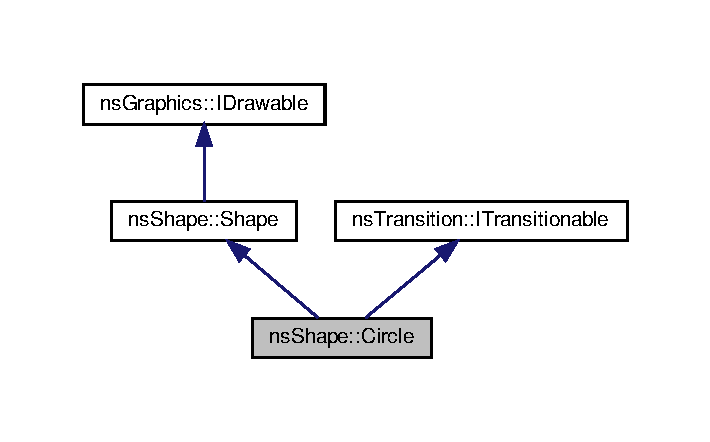
\includegraphics[width=341pt]{classns_shape_1_1_circle__inherit__graph}
\end{center}
\end{figure}


Collaboration diagram for ns\+Shape\+:\+:Circle\+:
\nopagebreak
\begin{figure}[H]
\begin{center}
\leavevmode
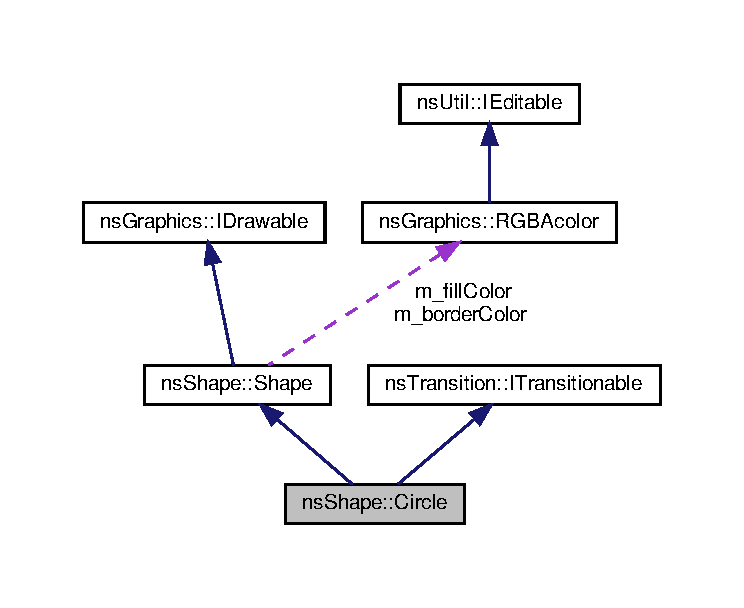
\includegraphics[width=350pt]{classns_shape_1_1_circle__coll__graph}
\end{center}
\end{figure}
\subsection*{Public Types}
\begin{DoxyCompactItemize}
\item 
enum \hyperlink{classns_shape_1_1_circle_a65ce20b6f5c10a111c1542f06154a235}{Transition\+Ids} \{ \newline
\hyperlink{classns_shape_1_1_circle_a65ce20b6f5c10a111c1542f06154a235a9fe224767a5f886c96a3f23e6355677a}{T\+R\+A\+N\+S\+I\+T\+I\+O\+N\+\_\+\+F\+I\+L\+L\+\_\+\+C\+O\+L\+O\+R\+\_\+\+R\+GB}, 
\hyperlink{classns_shape_1_1_circle_a65ce20b6f5c10a111c1542f06154a235a0df548537c2bd5e8aad51eab0a182d08}{T\+R\+A\+N\+S\+I\+T\+I\+O\+N\+\_\+\+F\+I\+L\+L\+\_\+\+C\+O\+L\+O\+R\+\_\+\+A\+L\+P\+HA}, 
\hyperlink{classns_shape_1_1_circle_a65ce20b6f5c10a111c1542f06154a235a2fdc553c832dfca9e296d9775c107732}{T\+R\+A\+N\+S\+I\+T\+I\+O\+N\+\_\+\+B\+O\+R\+D\+E\+R\+\_\+\+C\+O\+L\+O\+R\+\_\+\+R\+GB}, 
\hyperlink{classns_shape_1_1_circle_a65ce20b6f5c10a111c1542f06154a235a07cbcb4b2a43a087c534998e1ca553ee}{T\+R\+A\+N\+S\+I\+T\+I\+O\+N\+\_\+\+B\+O\+R\+D\+E\+R\+\_\+\+C\+O\+L\+O\+R\+\_\+\+A\+L\+P\+HA}, 
\newline
\hyperlink{classns_shape_1_1_circle_a65ce20b6f5c10a111c1542f06154a235aa2a6bbdede0b294813c638e4359c8603}{T\+R\+A\+N\+S\+I\+T\+I\+O\+N\+\_\+\+P\+O\+S\+I\+T\+I\+ON}, 
\hyperlink{classns_shape_1_1_circle_a65ce20b6f5c10a111c1542f06154a235a8a3d4b3560b97d5e11b81b58e2808393}{T\+R\+A\+N\+S\+I\+T\+I\+O\+N\+\_\+\+R\+A\+D\+I\+US}
 \}\begin{DoxyCompactList}\small\item\em Transition\+Ids \+: Liste de toutes les transitions que cet élément peut exécuter. \end{DoxyCompactList}
\end{DoxyCompactItemize}
\subsection*{Public Member Functions}
\begin{DoxyCompactItemize}
\item 
\hyperlink{classns_shape_1_1_circle_a06b1c1c7ea1e4ec8228d929e7b3966ee}{Circle} (const \hyperlink{classns_graphics_1_1_vec2_d}{ns\+Graphics\+::\+Vec2D} \&position, const unsigned \&radius, const \hyperlink{classns_graphics_1_1_r_g_b_acolor}{ns\+Graphics\+::\+R\+G\+B\+Acolor} \&fill\+Color, const \hyperlink{classns_graphics_1_1_r_g_b_acolor}{ns\+Graphics\+::\+R\+G\+B\+Acolor} \&border\+Color=\hyperlink{namespacens_graphics_ab2001ad03cceb2565849e04465618c1e}{ns\+Graphics\+::\+K\+Transparent})
\begin{DoxyCompactList}\small\item\em Constructeur pour la classe \hyperlink{classns_shape_1_1_circle}{Circle}. \end{DoxyCompactList}\item 
virtual \hyperlink{classns_shape_1_1_circle_a2446e688c063dcb2693adfcfacbb2804}{$\sim$\+Circle} () override=default
\begin{DoxyCompactList}\small\item\em Destructeur virtuel pour la classe \hyperlink{classns_shape_1_1_circle}{Circle}. \end{DoxyCompactList}\item 
virtual void \hyperlink{classns_shape_1_1_circle_a279581f6104719395091039cea1707e5}{draw} (\hyperlink{class_min_g_l}{Min\+GL} \&window) const override
\begin{DoxyCompactList}\small\item\em Fonction pour afficher l\textquotesingle{}objet. \end{DoxyCompactList}\item 
virtual void \hyperlink{classns_shape_1_1_circle_a2d126b4d87ea0b141cf1bac7150f760e}{get\+Values} (const int \&id, std\+::vector$<$ float $>$ \&values) override
\begin{DoxyCompactList}\small\item\em Récupère des valeurs dans un vecteur de float pour l\textquotesingle{}ID spécifié \end{DoxyCompactList}\item 
virtual void \hyperlink{classns_shape_1_1_circle_a3edfd0468ef78f456c4fc4fd57c84cdf}{set\+Values} (const int \&id, const std\+::vector$<$ float $>$ \&values) override
\begin{DoxyCompactList}\small\item\em Définit les nouvelles valeurs pour l\textquotesingle{}ID spécifié \end{DoxyCompactList}\item 
\hyperlink{classns_shape_1_1_circle}{Circle} \hyperlink{classns_shape_1_1_circle_a8b1f88a61fb38c283b11600e4eec6fe3}{operator+} (const \hyperlink{classns_graphics_1_1_vec2_d}{ns\+Graphics\+::\+Vec2D} \&\hyperlink{classns_shape_1_1_circle_a85b4102c4a23101fba4f90c1f8e84168}{get\+Position}) const
\begin{DoxyCompactList}\small\item\em Opérateur de décalage. \end{DoxyCompactList}\item 
\hyperlink{classns_shape_1_1_circle}{Circle} \hyperlink{classns_shape_1_1_circle_ad34827f3120b9331389a00cbf02468cb}{operator$\ast$} (const float \&f) const
\begin{DoxyCompactList}\small\item\em Opérateur de réduction. \end{DoxyCompactList}\item 
const \hyperlink{classns_graphics_1_1_vec2_d}{ns\+Graphics\+::\+Vec2D} \& \hyperlink{classns_shape_1_1_circle_a85b4102c4a23101fba4f90c1f8e84168}{get\+Position} () const
\begin{DoxyCompactList}\small\item\em Récupère la position du cercle. \end{DoxyCompactList}\item 
void \hyperlink{classns_shape_1_1_circle_ac4e73227c9ec7e22670bd012b6f37bef}{set\+Position} (const \hyperlink{classns_graphics_1_1_vec2_d}{ns\+Graphics\+::\+Vec2D} \&position)
\begin{DoxyCompactList}\small\item\em Définit la nouvelle position du cercle. \end{DoxyCompactList}\item 
unsigned \hyperlink{classns_shape_1_1_circle_afcb275822a67ec49167fe122ab74872c}{get\+Radius} () const
\begin{DoxyCompactList}\small\item\em Récupère le rayon du cercle. \end{DoxyCompactList}\item 
void \hyperlink{classns_shape_1_1_circle_a5f20408e41621d21487b6162eabc3a7d}{set\+Radius} (const unsigned \&radius)
\begin{DoxyCompactList}\small\item\em Définit le nouveau rayon du cercle. \end{DoxyCompactList}\end{DoxyCompactItemize}
\subsection*{Additional Inherited Members}


\subsection{Detailed Description}
Classe représentant un cercle. 

Definition at line 25 of file circle.\+h.



\subsection{Member Enumeration Documentation}
\mbox{\Hypertarget{classns_shape_1_1_circle_a65ce20b6f5c10a111c1542f06154a235}\label{classns_shape_1_1_circle_a65ce20b6f5c10a111c1542f06154a235}} 
\index{ns\+Shape\+::\+Circle@{ns\+Shape\+::\+Circle}!Transition\+Ids@{Transition\+Ids}}
\index{Transition\+Ids@{Transition\+Ids}!ns\+Shape\+::\+Circle@{ns\+Shape\+::\+Circle}}
\subsubsection{\texorpdfstring{Transition\+Ids}{TransitionIds}}
{\footnotesize\ttfamily enum \hyperlink{classns_shape_1_1_circle_a65ce20b6f5c10a111c1542f06154a235}{ns\+Shape\+::\+Circle\+::\+Transition\+Ids}}



Transition\+Ids \+: Liste de toutes les transitions que cet élément peut exécuter. 

\begin{DoxyEnumFields}{Enumerator}
\raisebox{\heightof{T}}[0pt][0pt]{\index{T\+R\+A\+N\+S\+I\+T\+I\+O\+N\+\_\+\+F\+I\+L\+L\+\_\+\+C\+O\+L\+O\+R\+\_\+\+R\+GB@{T\+R\+A\+N\+S\+I\+T\+I\+O\+N\+\_\+\+F\+I\+L\+L\+\_\+\+C\+O\+L\+O\+R\+\_\+\+R\+GB}!ns\+Shape\+::\+Circle@{ns\+Shape\+::\+Circle}}\index{ns\+Shape\+::\+Circle@{ns\+Shape\+::\+Circle}!T\+R\+A\+N\+S\+I\+T\+I\+O\+N\+\_\+\+F\+I\+L\+L\+\_\+\+C\+O\+L\+O\+R\+\_\+\+R\+GB@{T\+R\+A\+N\+S\+I\+T\+I\+O\+N\+\_\+\+F\+I\+L\+L\+\_\+\+C\+O\+L\+O\+R\+\_\+\+R\+GB}}}\mbox{\Hypertarget{classns_shape_1_1_circle_a65ce20b6f5c10a111c1542f06154a235a9fe224767a5f886c96a3f23e6355677a}\label{classns_shape_1_1_circle_a65ce20b6f5c10a111c1542f06154a235a9fe224767a5f886c96a3f23e6355677a}} 
T\+R\+A\+N\+S\+I\+T\+I\+O\+N\+\_\+\+F\+I\+L\+L\+\_\+\+C\+O\+L\+O\+R\+\_\+\+R\+GB&Transition pour la couleur de remplissage \\
\hline

\raisebox{\heightof{T}}[0pt][0pt]{\index{T\+R\+A\+N\+S\+I\+T\+I\+O\+N\+\_\+\+F\+I\+L\+L\+\_\+\+C\+O\+L\+O\+R\+\_\+\+A\+L\+P\+HA@{T\+R\+A\+N\+S\+I\+T\+I\+O\+N\+\_\+\+F\+I\+L\+L\+\_\+\+C\+O\+L\+O\+R\+\_\+\+A\+L\+P\+HA}!ns\+Shape\+::\+Circle@{ns\+Shape\+::\+Circle}}\index{ns\+Shape\+::\+Circle@{ns\+Shape\+::\+Circle}!T\+R\+A\+N\+S\+I\+T\+I\+O\+N\+\_\+\+F\+I\+L\+L\+\_\+\+C\+O\+L\+O\+R\+\_\+\+A\+L\+P\+HA@{T\+R\+A\+N\+S\+I\+T\+I\+O\+N\+\_\+\+F\+I\+L\+L\+\_\+\+C\+O\+L\+O\+R\+\_\+\+A\+L\+P\+HA}}}\mbox{\Hypertarget{classns_shape_1_1_circle_a65ce20b6f5c10a111c1542f06154a235a0df548537c2bd5e8aad51eab0a182d08}\label{classns_shape_1_1_circle_a65ce20b6f5c10a111c1542f06154a235a0df548537c2bd5e8aad51eab0a182d08}} 
T\+R\+A\+N\+S\+I\+T\+I\+O\+N\+\_\+\+F\+I\+L\+L\+\_\+\+C\+O\+L\+O\+R\+\_\+\+A\+L\+P\+HA&Transition pour la transparence de remplissage \\
\hline

\raisebox{\heightof{T}}[0pt][0pt]{\index{T\+R\+A\+N\+S\+I\+T\+I\+O\+N\+\_\+\+B\+O\+R\+D\+E\+R\+\_\+\+C\+O\+L\+O\+R\+\_\+\+R\+GB@{T\+R\+A\+N\+S\+I\+T\+I\+O\+N\+\_\+\+B\+O\+R\+D\+E\+R\+\_\+\+C\+O\+L\+O\+R\+\_\+\+R\+GB}!ns\+Shape\+::\+Circle@{ns\+Shape\+::\+Circle}}\index{ns\+Shape\+::\+Circle@{ns\+Shape\+::\+Circle}!T\+R\+A\+N\+S\+I\+T\+I\+O\+N\+\_\+\+B\+O\+R\+D\+E\+R\+\_\+\+C\+O\+L\+O\+R\+\_\+\+R\+GB@{T\+R\+A\+N\+S\+I\+T\+I\+O\+N\+\_\+\+B\+O\+R\+D\+E\+R\+\_\+\+C\+O\+L\+O\+R\+\_\+\+R\+GB}}}\mbox{\Hypertarget{classns_shape_1_1_circle_a65ce20b6f5c10a111c1542f06154a235a2fdc553c832dfca9e296d9775c107732}\label{classns_shape_1_1_circle_a65ce20b6f5c10a111c1542f06154a235a2fdc553c832dfca9e296d9775c107732}} 
T\+R\+A\+N\+S\+I\+T\+I\+O\+N\+\_\+\+B\+O\+R\+D\+E\+R\+\_\+\+C\+O\+L\+O\+R\+\_\+\+R\+GB&Transition pour la couleur de bord \\
\hline

\raisebox{\heightof{T}}[0pt][0pt]{\index{T\+R\+A\+N\+S\+I\+T\+I\+O\+N\+\_\+\+B\+O\+R\+D\+E\+R\+\_\+\+C\+O\+L\+O\+R\+\_\+\+A\+L\+P\+HA@{T\+R\+A\+N\+S\+I\+T\+I\+O\+N\+\_\+\+B\+O\+R\+D\+E\+R\+\_\+\+C\+O\+L\+O\+R\+\_\+\+A\+L\+P\+HA}!ns\+Shape\+::\+Circle@{ns\+Shape\+::\+Circle}}\index{ns\+Shape\+::\+Circle@{ns\+Shape\+::\+Circle}!T\+R\+A\+N\+S\+I\+T\+I\+O\+N\+\_\+\+B\+O\+R\+D\+E\+R\+\_\+\+C\+O\+L\+O\+R\+\_\+\+A\+L\+P\+HA@{T\+R\+A\+N\+S\+I\+T\+I\+O\+N\+\_\+\+B\+O\+R\+D\+E\+R\+\_\+\+C\+O\+L\+O\+R\+\_\+\+A\+L\+P\+HA}}}\mbox{\Hypertarget{classns_shape_1_1_circle_a65ce20b6f5c10a111c1542f06154a235a07cbcb4b2a43a087c534998e1ca553ee}\label{classns_shape_1_1_circle_a65ce20b6f5c10a111c1542f06154a235a07cbcb4b2a43a087c534998e1ca553ee}} 
T\+R\+A\+N\+S\+I\+T\+I\+O\+N\+\_\+\+B\+O\+R\+D\+E\+R\+\_\+\+C\+O\+L\+O\+R\+\_\+\+A\+L\+P\+HA&Transition pour la transparence de bord \\
\hline

\raisebox{\heightof{T}}[0pt][0pt]{\index{T\+R\+A\+N\+S\+I\+T\+I\+O\+N\+\_\+\+P\+O\+S\+I\+T\+I\+ON@{T\+R\+A\+N\+S\+I\+T\+I\+O\+N\+\_\+\+P\+O\+S\+I\+T\+I\+ON}!ns\+Shape\+::\+Circle@{ns\+Shape\+::\+Circle}}\index{ns\+Shape\+::\+Circle@{ns\+Shape\+::\+Circle}!T\+R\+A\+N\+S\+I\+T\+I\+O\+N\+\_\+\+P\+O\+S\+I\+T\+I\+ON@{T\+R\+A\+N\+S\+I\+T\+I\+O\+N\+\_\+\+P\+O\+S\+I\+T\+I\+ON}}}\mbox{\Hypertarget{classns_shape_1_1_circle_a65ce20b6f5c10a111c1542f06154a235aa2a6bbdede0b294813c638e4359c8603}\label{classns_shape_1_1_circle_a65ce20b6f5c10a111c1542f06154a235aa2a6bbdede0b294813c638e4359c8603}} 
T\+R\+A\+N\+S\+I\+T\+I\+O\+N\+\_\+\+P\+O\+S\+I\+T\+I\+ON&Transition pour la position \\
\hline

\raisebox{\heightof{T}}[0pt][0pt]{\index{T\+R\+A\+N\+S\+I\+T\+I\+O\+N\+\_\+\+R\+A\+D\+I\+US@{T\+R\+A\+N\+S\+I\+T\+I\+O\+N\+\_\+\+R\+A\+D\+I\+US}!ns\+Shape\+::\+Circle@{ns\+Shape\+::\+Circle}}\index{ns\+Shape\+::\+Circle@{ns\+Shape\+::\+Circle}!T\+R\+A\+N\+S\+I\+T\+I\+O\+N\+\_\+\+R\+A\+D\+I\+US@{T\+R\+A\+N\+S\+I\+T\+I\+O\+N\+\_\+\+R\+A\+D\+I\+US}}}\mbox{\Hypertarget{classns_shape_1_1_circle_a65ce20b6f5c10a111c1542f06154a235a8a3d4b3560b97d5e11b81b58e2808393}\label{classns_shape_1_1_circle_a65ce20b6f5c10a111c1542f06154a235a8a3d4b3560b97d5e11b81b58e2808393}} 
T\+R\+A\+N\+S\+I\+T\+I\+O\+N\+\_\+\+R\+A\+D\+I\+US&Transition pour le rayon \\
\hline

\end{DoxyEnumFields}


Definition at line 32 of file circle.\+h.



\subsection{Constructor \& Destructor Documentation}
\mbox{\Hypertarget{classns_shape_1_1_circle_a06b1c1c7ea1e4ec8228d929e7b3966ee}\label{classns_shape_1_1_circle_a06b1c1c7ea1e4ec8228d929e7b3966ee}} 
\index{ns\+Shape\+::\+Circle@{ns\+Shape\+::\+Circle}!Circle@{Circle}}
\index{Circle@{Circle}!ns\+Shape\+::\+Circle@{ns\+Shape\+::\+Circle}}
\subsubsection{\texorpdfstring{Circle()}{Circle()}}
{\footnotesize\ttfamily ns\+Shape\+::\+Circle\+::\+Circle (\begin{DoxyParamCaption}\item[{const \hyperlink{classns_graphics_1_1_vec2_d}{ns\+Graphics\+::\+Vec2D} \&}]{position,  }\item[{const unsigned \&}]{radius,  }\item[{const \hyperlink{classns_graphics_1_1_r_g_b_acolor}{ns\+Graphics\+::\+R\+G\+B\+Acolor} \&}]{fill\+Color,  }\item[{const \hyperlink{classns_graphics_1_1_r_g_b_acolor}{ns\+Graphics\+::\+R\+G\+B\+Acolor} \&}]{border\+Color = {\ttfamily \hyperlink{namespacens_graphics_ab2001ad03cceb2565849e04465618c1e}{ns\+Graphics\+::\+K\+Transparent}} }\end{DoxyParamCaption})}



Constructeur pour la classe \hyperlink{classns_shape_1_1_circle}{Circle}. 


\begin{DoxyParams}[1]{Parameters}
\mbox{\tt in}  & {\em first\+Position} & \+: Position du centre \\
\hline
\mbox{\tt in}  & {\em radius} & \+: Rayon du cercle \\
\hline
\mbox{\tt in}  & {\em fill\+Color} & \+: Couleur de remplissage \\
\hline
\mbox{\tt in}  & {\em border\+Color} & \+: Couleur de bord \\
\hline
\end{DoxyParams}
\mbox{\Hypertarget{classns_shape_1_1_circle_a2446e688c063dcb2693adfcfacbb2804}\label{classns_shape_1_1_circle_a2446e688c063dcb2693adfcfacbb2804}} 
\index{ns\+Shape\+::\+Circle@{ns\+Shape\+::\+Circle}!````~Circle@{$\sim$\+Circle}}
\index{````~Circle@{$\sim$\+Circle}!ns\+Shape\+::\+Circle@{ns\+Shape\+::\+Circle}}
\subsubsection{\texorpdfstring{$\sim$\+Circle()}{~Circle()}}
{\footnotesize\ttfamily ns\+Shape\+::\+Circle\+::$\sim$\+Circle (\begin{DoxyParamCaption}{ }\end{DoxyParamCaption})\hspace{0.3cm}{\ttfamily [override]}, {\ttfamily [virtual]}, {\ttfamily [default]}}



Destructeur virtuel pour la classe \hyperlink{classns_shape_1_1_circle}{Circle}. 



\subsection{Member Function Documentation}
\mbox{\Hypertarget{classns_shape_1_1_circle_a279581f6104719395091039cea1707e5}\label{classns_shape_1_1_circle_a279581f6104719395091039cea1707e5}} 
\index{ns\+Shape\+::\+Circle@{ns\+Shape\+::\+Circle}!draw@{draw}}
\index{draw@{draw}!ns\+Shape\+::\+Circle@{ns\+Shape\+::\+Circle}}
\subsubsection{\texorpdfstring{draw()}{draw()}}
{\footnotesize\ttfamily virtual void ns\+Shape\+::\+Circle\+::draw (\begin{DoxyParamCaption}\item[{\hyperlink{class_min_g_l}{Min\+GL} \&}]{window }\end{DoxyParamCaption}) const\hspace{0.3cm}{\ttfamily [override]}, {\ttfamily [virtual]}}



Fonction pour afficher l\textquotesingle{}objet. 



Implements \hyperlink{classns_graphics_1_1_i_drawable_abed8a61e1d507d31e76f0891f3bf9c51}{ns\+Graphics\+::\+I\+Drawable}.

\mbox{\Hypertarget{classns_shape_1_1_circle_a85b4102c4a23101fba4f90c1f8e84168}\label{classns_shape_1_1_circle_a85b4102c4a23101fba4f90c1f8e84168}} 
\index{ns\+Shape\+::\+Circle@{ns\+Shape\+::\+Circle}!get\+Position@{get\+Position}}
\index{get\+Position@{get\+Position}!ns\+Shape\+::\+Circle@{ns\+Shape\+::\+Circle}}
\subsubsection{\texorpdfstring{get\+Position()}{getPosition()}}
{\footnotesize\ttfamily const \hyperlink{classns_graphics_1_1_vec2_d}{ns\+Graphics\+::\+Vec2D} \& ns\+Shape\+::\+Circle\+::get\+Position (\begin{DoxyParamCaption}{ }\end{DoxyParamCaption}) const}



Récupère la position du cercle. 

\mbox{\Hypertarget{classns_shape_1_1_circle_afcb275822a67ec49167fe122ab74872c}\label{classns_shape_1_1_circle_afcb275822a67ec49167fe122ab74872c}} 
\index{ns\+Shape\+::\+Circle@{ns\+Shape\+::\+Circle}!get\+Radius@{get\+Radius}}
\index{get\+Radius@{get\+Radius}!ns\+Shape\+::\+Circle@{ns\+Shape\+::\+Circle}}
\subsubsection{\texorpdfstring{get\+Radius()}{getRadius()}}
{\footnotesize\ttfamily unsigned ns\+Shape\+::\+Circle\+::get\+Radius (\begin{DoxyParamCaption}{ }\end{DoxyParamCaption}) const}



Récupère le rayon du cercle. 

\mbox{\Hypertarget{classns_shape_1_1_circle_a2d126b4d87ea0b141cf1bac7150f760e}\label{classns_shape_1_1_circle_a2d126b4d87ea0b141cf1bac7150f760e}} 
\index{ns\+Shape\+::\+Circle@{ns\+Shape\+::\+Circle}!get\+Values@{get\+Values}}
\index{get\+Values@{get\+Values}!ns\+Shape\+::\+Circle@{ns\+Shape\+::\+Circle}}
\subsubsection{\texorpdfstring{get\+Values()}{getValues()}}
{\footnotesize\ttfamily virtual void ns\+Shape\+::\+Circle\+::get\+Values (\begin{DoxyParamCaption}\item[{const int \&}]{id,  }\item[{std\+::vector$<$ float $>$ \&}]{values }\end{DoxyParamCaption})\hspace{0.3cm}{\ttfamily [override]}, {\ttfamily [virtual]}}



Récupère des valeurs dans un vecteur de float pour l\textquotesingle{}ID spécifié 


\begin{DoxyParams}[1]{Parameters}
\mbox{\tt in}  & {\em id} & ID des valeurs a récupérer \\
\hline
\mbox{\tt in,out}  & {\em values} & Vecteur de valeurs a peupler \\
\hline
\end{DoxyParams}


Implements \hyperlink{classns_transition_1_1_i_transitionable_a5871a16fd47c1e5c8bacdd5da8597ed9}{ns\+Transition\+::\+I\+Transitionable}.

\mbox{\Hypertarget{classns_shape_1_1_circle_ad34827f3120b9331389a00cbf02468cb}\label{classns_shape_1_1_circle_ad34827f3120b9331389a00cbf02468cb}} 
\index{ns\+Shape\+::\+Circle@{ns\+Shape\+::\+Circle}!operator$\ast$@{operator$\ast$}}
\index{operator$\ast$@{operator$\ast$}!ns\+Shape\+::\+Circle@{ns\+Shape\+::\+Circle}}
\subsubsection{\texorpdfstring{operator$\ast$()}{operator*()}}
{\footnotesize\ttfamily \hyperlink{classns_shape_1_1_circle}{Circle} ns\+Shape\+::\+Circle\+::operator$\ast$ (\begin{DoxyParamCaption}\item[{const float \&}]{f }\end{DoxyParamCaption}) const}



Opérateur de réduction. 


\begin{DoxyParams}[1]{Parameters}
\mbox{\tt in}  & {\em f} & \+: Nombre avec lequel multiplier la position actuelle \\
\hline
\end{DoxyParams}
\mbox{\Hypertarget{classns_shape_1_1_circle_a8b1f88a61fb38c283b11600e4eec6fe3}\label{classns_shape_1_1_circle_a8b1f88a61fb38c283b11600e4eec6fe3}} 
\index{ns\+Shape\+::\+Circle@{ns\+Shape\+::\+Circle}!operator+@{operator+}}
\index{operator+@{operator+}!ns\+Shape\+::\+Circle@{ns\+Shape\+::\+Circle}}
\subsubsection{\texorpdfstring{operator+()}{operator+()}}
{\footnotesize\ttfamily \hyperlink{classns_shape_1_1_circle}{Circle} ns\+Shape\+::\+Circle\+::operator+ (\begin{DoxyParamCaption}\item[{const \hyperlink{classns_graphics_1_1_vec2_d}{ns\+Graphics\+::\+Vec2D} \&}]{position }\end{DoxyParamCaption}) const}



Opérateur de décalage. 


\begin{DoxyParams}[1]{Parameters}
\mbox{\tt in}  & {\em position} & \+: Position a additionner \\
\hline
\end{DoxyParams}
\mbox{\Hypertarget{classns_shape_1_1_circle_ac4e73227c9ec7e22670bd012b6f37bef}\label{classns_shape_1_1_circle_ac4e73227c9ec7e22670bd012b6f37bef}} 
\index{ns\+Shape\+::\+Circle@{ns\+Shape\+::\+Circle}!set\+Position@{set\+Position}}
\index{set\+Position@{set\+Position}!ns\+Shape\+::\+Circle@{ns\+Shape\+::\+Circle}}
\subsubsection{\texorpdfstring{set\+Position()}{setPosition()}}
{\footnotesize\ttfamily void ns\+Shape\+::\+Circle\+::set\+Position (\begin{DoxyParamCaption}\item[{const \hyperlink{classns_graphics_1_1_vec2_d}{ns\+Graphics\+::\+Vec2D} \&}]{position }\end{DoxyParamCaption})}



Définit la nouvelle position du cercle. 


\begin{DoxyParams}[1]{Parameters}
\mbox{\tt in}  & {\em position} & \+: Nouvelle position \\
\hline
\end{DoxyParams}
\mbox{\Hypertarget{classns_shape_1_1_circle_a5f20408e41621d21487b6162eabc3a7d}\label{classns_shape_1_1_circle_a5f20408e41621d21487b6162eabc3a7d}} 
\index{ns\+Shape\+::\+Circle@{ns\+Shape\+::\+Circle}!set\+Radius@{set\+Radius}}
\index{set\+Radius@{set\+Radius}!ns\+Shape\+::\+Circle@{ns\+Shape\+::\+Circle}}
\subsubsection{\texorpdfstring{set\+Radius()}{setRadius()}}
{\footnotesize\ttfamily void ns\+Shape\+::\+Circle\+::set\+Radius (\begin{DoxyParamCaption}\item[{const unsigned \&}]{radius }\end{DoxyParamCaption})}



Définit le nouveau rayon du cercle. 


\begin{DoxyParams}[1]{Parameters}
\mbox{\tt in}  & {\em radius} & \+: Nouveau rayon \\
\hline
\end{DoxyParams}
\mbox{\Hypertarget{classns_shape_1_1_circle_a3edfd0468ef78f456c4fc4fd57c84cdf}\label{classns_shape_1_1_circle_a3edfd0468ef78f456c4fc4fd57c84cdf}} 
\index{ns\+Shape\+::\+Circle@{ns\+Shape\+::\+Circle}!set\+Values@{set\+Values}}
\index{set\+Values@{set\+Values}!ns\+Shape\+::\+Circle@{ns\+Shape\+::\+Circle}}
\subsubsection{\texorpdfstring{set\+Values()}{setValues()}}
{\footnotesize\ttfamily virtual void ns\+Shape\+::\+Circle\+::set\+Values (\begin{DoxyParamCaption}\item[{const int \&}]{id,  }\item[{const std\+::vector$<$ float $>$ \&}]{values }\end{DoxyParamCaption})\hspace{0.3cm}{\ttfamily [override]}, {\ttfamily [virtual]}}



Définit les nouvelles valeurs pour l\textquotesingle{}ID spécifié 


\begin{DoxyParams}[1]{Parameters}
\mbox{\tt in}  & {\em id} & ID des valeurs a définir \\
\hline
\mbox{\tt in}  & {\em values} & Vecteur des nouvelles valeurs a appliquer \\
\hline
\end{DoxyParams}


Implements \hyperlink{classns_transition_1_1_i_transitionable_ade37d29f7f2ca4890ed0e2e64d033197}{ns\+Transition\+::\+I\+Transitionable}.



The documentation for this class was generated from the following file\+:\begin{DoxyCompactItemize}
\item 
libs/mingl/shape/\hyperlink{circle_8h}{circle.\+h}\end{DoxyCompactItemize}

\hypertarget{structenemy_1_1_enemy}{}\section{enemy\+:\+:Enemy Struct Reference}
\label{structenemy_1_1_enemy}\index{enemy\+::\+Enemy@{enemy\+::\+Enemy}}


Structure d\textquotesingle{}enemies.  




{\ttfamily \#include $<$enemy.\+h$>$}



Collaboration diagram for enemy\+:\+:Enemy\+:
\nopagebreak
\begin{figure}[H]
\begin{center}
\leavevmode
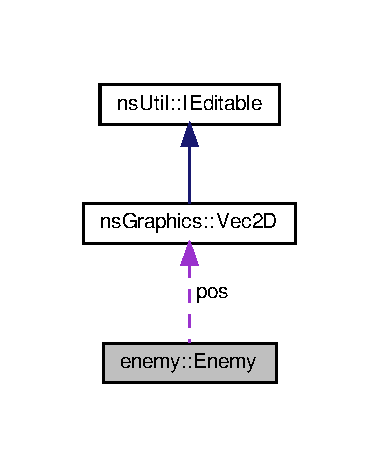
\includegraphics[width=182pt]{structenemy_1_1_enemy__coll__graph}
\end{center}
\end{figure}
\subsection*{Public Member Functions}
\begin{DoxyCompactItemize}
\item 
\hyperlink{structenemy_1_1_enemy_aee2b396985788d712cd905a7a827e557}{Enemy} (\hyperlink{classns_graphics_1_1_vec2_d}{ns\+Graphics\+::\+Vec2D} ent\+Pos, char ent\+Way)
\begin{DoxyCompactList}\small\item\em Fonction constructeur de la struct \hyperlink{structenemy_1_1_enemy}{Enemy}. \end{DoxyCompactList}\item 
void \hyperlink{structenemy_1_1_enemy_a56f663147f0dcfc4c6af07027713ba00}{update} (std\+::vector$<$ \hyperlink{structenemy_1_1_enemy}{Enemy} $>$ \&\hyperlink{multi_8cpp_a68dfd8cc6c330a8d7be4cf2f3a6892f3}{enemies}, std\+::vector$<$ \hyperlink{structtorpedo_1_1_torpedo}{torpedo\+::\+Torpedo} $>$ \&\hyperlink{multi_8cpp_a8d978ee3afff71f0b07f921403c2b403}{torpedos}, \hyperlink{class_min_g_l}{Min\+GL} \&window)
\begin{DoxyCompactList}\small\item\em Fonction de mise à jour des enemies (déplacement et tir) \end{DoxyCompactList}\item 
void \hyperlink{structenemy_1_1_enemy_aca9d44d3ae82ec9177f4d50760f0d1cc}{show} (\hyperlink{class_min_g_l}{Min\+GL} \&window)
\begin{DoxyCompactList}\small\item\em Rendu de l\textquotesingle{}enemie. \end{DoxyCompactList}\end{DoxyCompactItemize}
\subsection*{Public Attributes}
\begin{DoxyCompactItemize}
\item 
\hyperlink{classns_graphics_1_1_vec2_d}{ns\+Graphics\+::\+Vec2D} \hyperlink{structenemy_1_1_enemy_a1439cd408ff71d897e2414c062a3dda4}{pos}
\item 
bool \hyperlink{structenemy_1_1_enemy_ac64a666df47674ecf4abeb467991e5cb}{alive} = true
\item 
std\+::vector$<$ unsigned long $>$ \hyperlink{structenemy_1_1_enemy_aa59e1afdd7cba4658530a57b10152686}{size}
\item 
bool \hyperlink{structenemy_1_1_enemy_a03df75f44cf09e588c418e2b49388a9b}{go\+Down} = true
\item 
char \hyperlink{structenemy_1_1_enemy_a6b7b4f12f9ed4a167c1ed0444dda20ba}{way}
\end{DoxyCompactItemize}


\subsection{Detailed Description}
Structure d\textquotesingle{}enemies. 

Definition at line 35 of file enemy.\+h.



\subsection{Constructor \& Destructor Documentation}
\mbox{\Hypertarget{structenemy_1_1_enemy_aee2b396985788d712cd905a7a827e557}\label{structenemy_1_1_enemy_aee2b396985788d712cd905a7a827e557}} 
\index{enemy\+::\+Enemy@{enemy\+::\+Enemy}!Enemy@{Enemy}}
\index{Enemy@{Enemy}!enemy\+::\+Enemy@{enemy\+::\+Enemy}}
\subsubsection{\texorpdfstring{Enemy()}{Enemy()}}
{\footnotesize\ttfamily enemy\+::\+Enemy\+::\+Enemy (\begin{DoxyParamCaption}\item[{\hyperlink{classns_graphics_1_1_vec2_d}{ns\+Graphics\+::\+Vec2D}}]{ent\+Pos,  }\item[{char}]{ent\+Way }\end{DoxyParamCaption})}



Fonction constructeur de la struct \hyperlink{structenemy_1_1_enemy}{Enemy}. 


\begin{DoxyParams}[1]{Parameters}
\mbox{\tt in}  & {\em ent\+Pos} & \+: position du joueur \\
\hline
\mbox{\tt in}  & {\em ent\+Way} & \+: direction du joueur \\
\hline
\end{DoxyParams}


Definition at line 14 of file enemy.\+cpp.



\subsection{Member Function Documentation}
\mbox{\Hypertarget{structenemy_1_1_enemy_aca9d44d3ae82ec9177f4d50760f0d1cc}\label{structenemy_1_1_enemy_aca9d44d3ae82ec9177f4d50760f0d1cc}} 
\index{enemy\+::\+Enemy@{enemy\+::\+Enemy}!show@{show}}
\index{show@{show}!enemy\+::\+Enemy@{enemy\+::\+Enemy}}
\subsubsection{\texorpdfstring{show()}{show()}}
{\footnotesize\ttfamily void enemy\+::\+Enemy\+::show (\begin{DoxyParamCaption}\item[{\hyperlink{class_min_g_l}{Min\+GL} \&}]{window }\end{DoxyParamCaption})}



Rendu de l\textquotesingle{}enemie. 


\begin{DoxyParams}[1]{Parameters}
\mbox{\tt in,out}  & {\em window} & \+: fenêtre de jeu \\
\hline
\end{DoxyParams}


Definition at line 62 of file enemy.\+cpp.

\mbox{\Hypertarget{structenemy_1_1_enemy_a56f663147f0dcfc4c6af07027713ba00}\label{structenemy_1_1_enemy_a56f663147f0dcfc4c6af07027713ba00}} 
\index{enemy\+::\+Enemy@{enemy\+::\+Enemy}!update@{update}}
\index{update@{update}!enemy\+::\+Enemy@{enemy\+::\+Enemy}}
\subsubsection{\texorpdfstring{update()}{update()}}
{\footnotesize\ttfamily void enemy\+::\+Enemy\+::update (\begin{DoxyParamCaption}\item[{std\+::vector$<$ \hyperlink{structenemy_1_1_enemy}{Enemy} $>$ \&}]{enemies,  }\item[{std\+::vector$<$ \hyperlink{structtorpedo_1_1_torpedo}{torpedo\+::\+Torpedo} $>$ \&}]{torpedos,  }\item[{\hyperlink{class_min_g_l}{Min\+GL} \&}]{window }\end{DoxyParamCaption})}



Fonction de mise à jour des enemies (déplacement et tir) 


\begin{DoxyParams}[1]{Parameters}
\mbox{\tt in,out}  & {\em enemies} & \+: vecteur des enemies \\
\hline
\mbox{\tt in,out}  & {\em torpedos} & \+: vecteur des torpilles \\
\hline
\mbox{\tt in}  & {\em window} & \+: fenêtre de jeu \\
\hline
\end{DoxyParams}


Definition at line 21 of file enemy.\+cpp.



\subsection{Member Data Documentation}
\mbox{\Hypertarget{structenemy_1_1_enemy_ac64a666df47674ecf4abeb467991e5cb}\label{structenemy_1_1_enemy_ac64a666df47674ecf4abeb467991e5cb}} 
\index{enemy\+::\+Enemy@{enemy\+::\+Enemy}!alive@{alive}}
\index{alive@{alive}!enemy\+::\+Enemy@{enemy\+::\+Enemy}}
\subsubsection{\texorpdfstring{alive}{alive}}
{\footnotesize\ttfamily bool enemy\+::\+Enemy\+::alive = true}



Definition at line 39 of file enemy.\+h.

\mbox{\Hypertarget{structenemy_1_1_enemy_a03df75f44cf09e588c418e2b49388a9b}\label{structenemy_1_1_enemy_a03df75f44cf09e588c418e2b49388a9b}} 
\index{enemy\+::\+Enemy@{enemy\+::\+Enemy}!go\+Down@{go\+Down}}
\index{go\+Down@{go\+Down}!enemy\+::\+Enemy@{enemy\+::\+Enemy}}
\subsubsection{\texorpdfstring{go\+Down}{goDown}}
{\footnotesize\ttfamily bool enemy\+::\+Enemy\+::go\+Down = true}



Definition at line 41 of file enemy.\+h.

\mbox{\Hypertarget{structenemy_1_1_enemy_a1439cd408ff71d897e2414c062a3dda4}\label{structenemy_1_1_enemy_a1439cd408ff71d897e2414c062a3dda4}} 
\index{enemy\+::\+Enemy@{enemy\+::\+Enemy}!pos@{pos}}
\index{pos@{pos}!enemy\+::\+Enemy@{enemy\+::\+Enemy}}
\subsubsection{\texorpdfstring{pos}{pos}}
{\footnotesize\ttfamily \hyperlink{classns_graphics_1_1_vec2_d}{ns\+Graphics\+::\+Vec2D} enemy\+::\+Enemy\+::pos}



Definition at line 38 of file enemy.\+h.

\mbox{\Hypertarget{structenemy_1_1_enemy_aa59e1afdd7cba4658530a57b10152686}\label{structenemy_1_1_enemy_aa59e1afdd7cba4658530a57b10152686}} 
\index{enemy\+::\+Enemy@{enemy\+::\+Enemy}!size@{size}}
\index{size@{size}!enemy\+::\+Enemy@{enemy\+::\+Enemy}}
\subsubsection{\texorpdfstring{size}{size}}
{\footnotesize\ttfamily std\+::vector$<$unsigned long$>$ enemy\+::\+Enemy\+::size}



Definition at line 40 of file enemy.\+h.

\mbox{\Hypertarget{structenemy_1_1_enemy_a6b7b4f12f9ed4a167c1ed0444dda20ba}\label{structenemy_1_1_enemy_a6b7b4f12f9ed4a167c1ed0444dda20ba}} 
\index{enemy\+::\+Enemy@{enemy\+::\+Enemy}!way@{way}}
\index{way@{way}!enemy\+::\+Enemy@{enemy\+::\+Enemy}}
\subsubsection{\texorpdfstring{way}{way}}
{\footnotesize\ttfamily char enemy\+::\+Enemy\+::way}



Definition at line 42 of file enemy.\+h.



The documentation for this struct was generated from the following files\+:\begin{DoxyCompactItemize}
\item 
libs/game/entities/\hyperlink{enemy_8h}{enemy.\+h}\item 
src/entities/\hyperlink{enemy_8cpp}{enemy.\+cpp}\end{DoxyCompactItemize}

\hypertarget{structns_event_1_1_event__t}{}\section{ns\+Event\+:\+:Event\+\_\+t Struct Reference}
\label{structns_event_1_1_event__t}\index{ns\+Event\+::\+Event\+\_\+t@{ns\+Event\+::\+Event\+\_\+t}}


Possède des données pour un événement.  




{\ttfamily \#include $<$event.\+hpp$>$}



Collaboration diagram for ns\+Event\+:\+:Event\+\_\+t\+:
\nopagebreak
\begin{figure}[H]
\begin{center}
\leavevmode
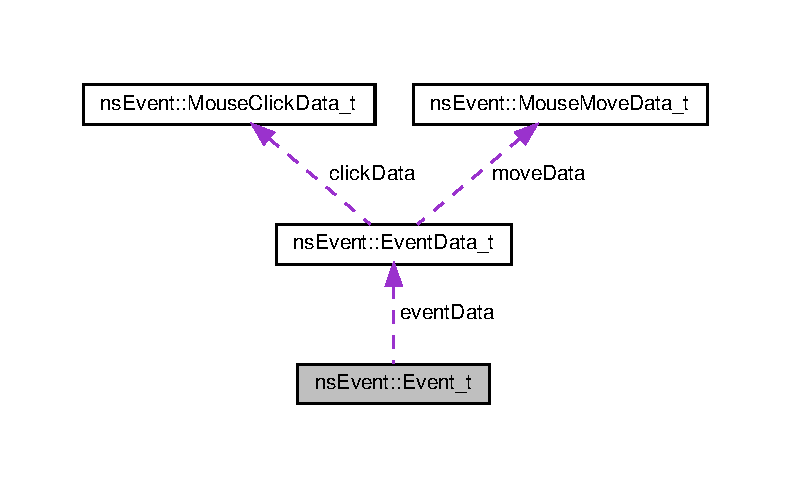
\includegraphics[width=350pt]{structns_event_1_1_event__t__coll__graph}
\end{center}
\end{figure}
\subsection*{Public Attributes}
\begin{DoxyCompactItemize}
\item 
\hyperlink{namespacens_event_a6e501b1114a041d127a56f51c66ada72}{Event\+Type\+\_\+t} \hyperlink{structns_event_1_1_event__t_a4658fcb9ee305cae39da30840d64192c}{event\+Type}
\item 
\hyperlink{unionns_event_1_1_event_data__t}{Event\+Data\+\_\+t} \hyperlink{structns_event_1_1_event__t_a148669454c11351db2ac902aad495ac8}{event\+Data}
\end{DoxyCompactItemize}


\subsection{Detailed Description}
Possède des données pour un événement. 

Definition at line 62 of file event.\+hpp.



\subsection{Member Data Documentation}
\mbox{\Hypertarget{structns_event_1_1_event__t_a148669454c11351db2ac902aad495ac8}\label{structns_event_1_1_event__t_a148669454c11351db2ac902aad495ac8}} 
\index{ns\+Event\+::\+Event\+\_\+t@{ns\+Event\+::\+Event\+\_\+t}!event\+Data@{event\+Data}}
\index{event\+Data@{event\+Data}!ns\+Event\+::\+Event\+\_\+t@{ns\+Event\+::\+Event\+\_\+t}}
\subsubsection{\texorpdfstring{event\+Data}{eventData}}
{\footnotesize\ttfamily \hyperlink{unionns_event_1_1_event_data__t}{Event\+Data\+\_\+t} ns\+Event\+::\+Event\+\_\+t\+::event\+Data}

Données de l\textquotesingle{}événement 

Definition at line 64 of file event.\+hpp.

\mbox{\Hypertarget{structns_event_1_1_event__t_a4658fcb9ee305cae39da30840d64192c}\label{structns_event_1_1_event__t_a4658fcb9ee305cae39da30840d64192c}} 
\index{ns\+Event\+::\+Event\+\_\+t@{ns\+Event\+::\+Event\+\_\+t}!event\+Type@{event\+Type}}
\index{event\+Type@{event\+Type}!ns\+Event\+::\+Event\+\_\+t@{ns\+Event\+::\+Event\+\_\+t}}
\subsubsection{\texorpdfstring{event\+Type}{eventType}}
{\footnotesize\ttfamily \hyperlink{namespacens_event_a6e501b1114a041d127a56f51c66ada72}{Event\+Type\+\_\+t} ns\+Event\+::\+Event\+\_\+t\+::event\+Type}

Type de l\textquotesingle{}événement 

Definition at line 63 of file event.\+hpp.



The documentation for this struct was generated from the following file\+:\begin{DoxyCompactItemize}
\item 
libs/mingl/event/\hyperlink{event_8hpp}{event.\+hpp}\end{DoxyCompactItemize}

\hypertarget{unionns_event_1_1_event_data__t}{}\section{ns\+Event\+:\+:Event\+Data\+\_\+t Union Reference}
\label{unionns_event_1_1_event_data__t}\index{ns\+Event\+::\+Event\+Data\+\_\+t@{ns\+Event\+::\+Event\+Data\+\_\+t}}


Union contenant les données d\textquotesingle{}un événement.  




{\ttfamily \#include $<$event.\+hpp$>$}



Collaboration diagram for ns\+Event\+:\+:Event\+Data\+\_\+t\+:
\nopagebreak
\begin{figure}[H]
\begin{center}
\leavevmode
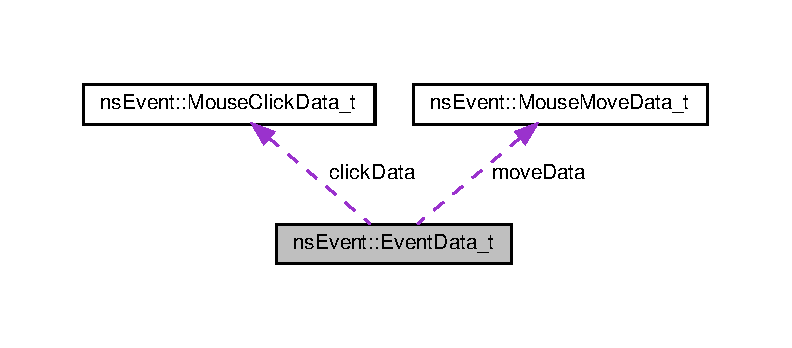
\includegraphics[width=350pt]{unionns_event_1_1_event_data__t__coll__graph}
\end{center}
\end{figure}
\subsection*{Public Attributes}
\begin{DoxyCompactItemize}
\item 
\hyperlink{structns_event_1_1_mouse_click_data__t}{Mouse\+Click\+Data\+\_\+t} \hyperlink{unionns_event_1_1_event_data__t_ac1478ee3007ce42a653e53c1200625bc}{click\+Data}
\item 
\hyperlink{structns_event_1_1_mouse_move_data__t}{Mouse\+Move\+Data\+\_\+t} \hyperlink{unionns_event_1_1_event_data__t_aac7ba31725a75d84fd32ea6a4d865a91}{move\+Data}
\end{DoxyCompactItemize}


\subsection{Detailed Description}
Union contenant les données d\textquotesingle{}un événement. 

Definition at line 53 of file event.\+hpp.



\subsection{Member Data Documentation}
\mbox{\Hypertarget{unionns_event_1_1_event_data__t_ac1478ee3007ce42a653e53c1200625bc}\label{unionns_event_1_1_event_data__t_ac1478ee3007ce42a653e53c1200625bc}} 
\index{ns\+Event\+::\+Event\+Data\+\_\+t@{ns\+Event\+::\+Event\+Data\+\_\+t}!click\+Data@{click\+Data}}
\index{click\+Data@{click\+Data}!ns\+Event\+::\+Event\+Data\+\_\+t@{ns\+Event\+::\+Event\+Data\+\_\+t}}
\subsubsection{\texorpdfstring{click\+Data}{clickData}}
{\footnotesize\ttfamily \hyperlink{structns_event_1_1_mouse_click_data__t}{Mouse\+Click\+Data\+\_\+t} ns\+Event\+::\+Event\+Data\+\_\+t\+::click\+Data}

Données pour un événement Mouse\+Click 

Definition at line 54 of file event.\+hpp.

\mbox{\Hypertarget{unionns_event_1_1_event_data__t_aac7ba31725a75d84fd32ea6a4d865a91}\label{unionns_event_1_1_event_data__t_aac7ba31725a75d84fd32ea6a4d865a91}} 
\index{ns\+Event\+::\+Event\+Data\+\_\+t@{ns\+Event\+::\+Event\+Data\+\_\+t}!move\+Data@{move\+Data}}
\index{move\+Data@{move\+Data}!ns\+Event\+::\+Event\+Data\+\_\+t@{ns\+Event\+::\+Event\+Data\+\_\+t}}
\subsubsection{\texorpdfstring{move\+Data}{moveData}}
{\footnotesize\ttfamily \hyperlink{structns_event_1_1_mouse_move_data__t}{Mouse\+Move\+Data\+\_\+t} ns\+Event\+::\+Event\+Data\+\_\+t\+::move\+Data}

Données pour un événment Mouse\+Move/\+Mouse\+Drag 

Definition at line 55 of file event.\+hpp.



The documentation for this union was generated from the following file\+:\begin{DoxyCompactItemize}
\item 
libs/mingl/event/\hyperlink{event_8hpp}{event.\+hpp}\end{DoxyCompactItemize}

\hypertarget{classns_event_1_1_event_manager}{}\section{ns\+Event\+:\+:Event\+Manager Class Reference}
\label{classns_event_1_1_event_manager}\index{ns\+Event\+::\+Event\+Manager@{ns\+Event\+::\+Event\+Manager}}


Gère une queue d\textquotesingle{}événement entrants.  




{\ttfamily \#include $<$event\+\_\+manager.\+h$>$}

\subsection*{Public Member Functions}
\begin{DoxyCompactItemize}
\item 
bool \hyperlink{classns_event_1_1_event_manager_a5a3119d969a296b8e94f223171fdf2e6}{has\+Event} ()
\begin{DoxyCompactList}\small\item\em Vérifie si un événement doit être traité \end{DoxyCompactList}\item 
void \hyperlink{classns_event_1_1_event_manager_a1eff8398ddb0a25da82e52a1067b85b5}{push\+Event} (const \hyperlink{structns_event_1_1_event__t}{Event\+\_\+t} \&event)
\begin{DoxyCompactList}\small\item\em Pousse un nouvel événement dans la queue. \end{DoxyCompactList}\item 
const \hyperlink{structns_event_1_1_event__t}{Event\+\_\+t} \hyperlink{classns_event_1_1_event_manager_ac37f8ed34ab7c874ff28af7dccc035f3}{pull\+Event} ()
\begin{DoxyCompactList}\small\item\em Tire l\textquotesingle{}événement le plus ancien, et l\textquotesingle{}enlève de la queue. \end{DoxyCompactList}\item 
void \hyperlink{classns_event_1_1_event_manager_adbc5ced9a9435f61f58436ff613632b4}{clear\+Events} ()
\begin{DoxyCompactList}\small\item\em Vide la queue. \end{DoxyCompactList}\end{DoxyCompactItemize}


\subsection{Detailed Description}
Gère une queue d\textquotesingle{}événement entrants. 

Definition at line 24 of file event\+\_\+manager.\+h.



\subsection{Member Function Documentation}
\mbox{\Hypertarget{classns_event_1_1_event_manager_adbc5ced9a9435f61f58436ff613632b4}\label{classns_event_1_1_event_manager_adbc5ced9a9435f61f58436ff613632b4}} 
\index{ns\+Event\+::\+Event\+Manager@{ns\+Event\+::\+Event\+Manager}!clear\+Events@{clear\+Events}}
\index{clear\+Events@{clear\+Events}!ns\+Event\+::\+Event\+Manager@{ns\+Event\+::\+Event\+Manager}}
\subsubsection{\texorpdfstring{clear\+Events()}{clearEvents()}}
{\footnotesize\ttfamily void ns\+Event\+::\+Event\+Manager\+::clear\+Events (\begin{DoxyParamCaption}{ }\end{DoxyParamCaption})}



Vide la queue. 

\mbox{\Hypertarget{classns_event_1_1_event_manager_a5a3119d969a296b8e94f223171fdf2e6}\label{classns_event_1_1_event_manager_a5a3119d969a296b8e94f223171fdf2e6}} 
\index{ns\+Event\+::\+Event\+Manager@{ns\+Event\+::\+Event\+Manager}!has\+Event@{has\+Event}}
\index{has\+Event@{has\+Event}!ns\+Event\+::\+Event\+Manager@{ns\+Event\+::\+Event\+Manager}}
\subsubsection{\texorpdfstring{has\+Event()}{hasEvent()}}
{\footnotesize\ttfamily bool ns\+Event\+::\+Event\+Manager\+::has\+Event (\begin{DoxyParamCaption}{ }\end{DoxyParamCaption})}



Vérifie si un événement doit être traité 

\begin{DoxyReturn}{Returns}
Si la queue possède au moins un élément 
\end{DoxyReturn}
\mbox{\Hypertarget{classns_event_1_1_event_manager_ac37f8ed34ab7c874ff28af7dccc035f3}\label{classns_event_1_1_event_manager_ac37f8ed34ab7c874ff28af7dccc035f3}} 
\index{ns\+Event\+::\+Event\+Manager@{ns\+Event\+::\+Event\+Manager}!pull\+Event@{pull\+Event}}
\index{pull\+Event@{pull\+Event}!ns\+Event\+::\+Event\+Manager@{ns\+Event\+::\+Event\+Manager}}
\subsubsection{\texorpdfstring{pull\+Event()}{pullEvent()}}
{\footnotesize\ttfamily const \hyperlink{structns_event_1_1_event__t}{Event\+\_\+t} ns\+Event\+::\+Event\+Manager\+::pull\+Event (\begin{DoxyParamCaption}{ }\end{DoxyParamCaption})}



Tire l\textquotesingle{}événement le plus ancien, et l\textquotesingle{}enlève de la queue. 

\begin{DoxyReturn}{Returns}
Une copie du plus ancien événement 
\end{DoxyReturn}
\mbox{\Hypertarget{classns_event_1_1_event_manager_a1eff8398ddb0a25da82e52a1067b85b5}\label{classns_event_1_1_event_manager_a1eff8398ddb0a25da82e52a1067b85b5}} 
\index{ns\+Event\+::\+Event\+Manager@{ns\+Event\+::\+Event\+Manager}!push\+Event@{push\+Event}}
\index{push\+Event@{push\+Event}!ns\+Event\+::\+Event\+Manager@{ns\+Event\+::\+Event\+Manager}}
\subsubsection{\texorpdfstring{push\+Event()}{pushEvent()}}
{\footnotesize\ttfamily void ns\+Event\+::\+Event\+Manager\+::push\+Event (\begin{DoxyParamCaption}\item[{const \hyperlink{structns_event_1_1_event__t}{Event\+\_\+t} \&}]{event }\end{DoxyParamCaption})}



Pousse un nouvel événement dans la queue. 


\begin{DoxyParams}[1]{Parameters}
\mbox{\tt in}  & {\em event} & \+: Evénement a pousser \\
\hline
\end{DoxyParams}


The documentation for this class was generated from the following file\+:\begin{DoxyCompactItemize}
\item 
libs/mingl/event/\hyperlink{event__manager_8h}{event\+\_\+manager.\+h}\end{DoxyCompactItemize}

\hypertarget{classns_gui_1_1_glut_font}{}\section{ns\+Gui\+:\+:Glut\+Font Class Reference}
\label{classns_gui_1_1_glut_font}\index{ns\+Gui\+::\+Glut\+Font@{ns\+Gui\+::\+Glut\+Font}}


Classe listant toute les polices rendues disponibles par Glut, a utiliser avec \hyperlink{classns_gui_1_1_text}{Text}.  




{\ttfamily \#include $<$glut\+\_\+font.\+h$>$}

\subsection*{Public Types}
\begin{DoxyCompactItemize}
\item 
enum \hyperlink{classns_gui_1_1_glut_font_aeeeb02d69e7dfc7e57957bd658c465ce}{Glut\+Fonts} \{ \newline
\hyperlink{classns_gui_1_1_glut_font_aeeeb02d69e7dfc7e57957bd658c465cea9c75a2a144604631db2af2ae284a9d82}{B\+I\+T\+M\+A\+P\+\_\+8\+\_\+\+B\+Y\+\_\+13}, 
\hyperlink{classns_gui_1_1_glut_font_aeeeb02d69e7dfc7e57957bd658c465ceafc7dc7274d17bd604f3cf91412650df0}{B\+I\+T\+M\+A\+P\+\_\+9\+\_\+\+B\+Y\+\_\+15}, 
\hyperlink{classns_gui_1_1_glut_font_aeeeb02d69e7dfc7e57957bd658c465cea35de9b7dc33c5aa8672423552fe83b38}{B\+I\+T\+M\+A\+P\+\_\+\+T\+I\+M\+E\+S\+\_\+\+R\+O\+M\+A\+N\+\_\+10}, 
\hyperlink{classns_gui_1_1_glut_font_aeeeb02d69e7dfc7e57957bd658c465cea466dd22d811df1310583c1a59d0103b0}{B\+I\+T\+M\+A\+P\+\_\+\+T\+I\+M\+E\+S\+\_\+\+R\+O\+M\+A\+N\+\_\+24}, 
\newline
\hyperlink{classns_gui_1_1_glut_font_aeeeb02d69e7dfc7e57957bd658c465ceae127744cea36edcff85327da64221d14}{B\+I\+T\+M\+A\+P\+\_\+\+H\+E\+L\+V\+E\+T\+I\+C\+A\+\_\+10}, 
\hyperlink{classns_gui_1_1_glut_font_aeeeb02d69e7dfc7e57957bd658c465ceab87b397237206af607190619163ec1e6}{B\+I\+T\+M\+A\+P\+\_\+\+H\+E\+L\+V\+E\+T\+I\+C\+A\+\_\+12}, 
\hyperlink{classns_gui_1_1_glut_font_aeeeb02d69e7dfc7e57957bd658c465cea11c7a92d3233d33d71de4ca2f0e27437}{B\+I\+T\+M\+A\+P\+\_\+\+H\+E\+L\+V\+E\+T\+I\+C\+A\+\_\+18}
 \}\begin{DoxyCompactList}\small\item\em Glut\+Fonts \+: Liste de toutes les polices Glut. \end{DoxyCompactList}
\end{DoxyCompactItemize}
\subsection*{Public Member Functions}
\begin{DoxyCompactItemize}
\item 
\hyperlink{classns_gui_1_1_glut_font_ac8e33c6ba8a95edcdcee4dd4d1a283ac}{Glut\+Font} (const \hyperlink{classns_gui_1_1_glut_font_aeeeb02d69e7dfc7e57957bd658c465ce}{Glut\+Fonts} \&font)
\begin{DoxyCompactList}\small\item\em Constructeur pour la classe \hyperlink{classns_gui_1_1_glut_font}{Glut\+Font}. \end{DoxyCompactList}\item 
void $\ast$ \hyperlink{classns_gui_1_1_glut_font_a10921b4183b246e9cfdebaca6b9e91a2}{convert\+For\+Glut} () const
\begin{DoxyCompactList}\small\item\em Récupère l\textquotesingle{}identificateur de police utilisable par Glut. \end{DoxyCompactList}\end{DoxyCompactItemize}


\subsection{Detailed Description}
Classe listant toute les polices rendues disponibles par Glut, a utiliser avec \hyperlink{classns_gui_1_1_text}{Text}. 

Definition at line 19 of file glut\+\_\+font.\+h.



\subsection{Member Enumeration Documentation}
\mbox{\Hypertarget{classns_gui_1_1_glut_font_aeeeb02d69e7dfc7e57957bd658c465ce}\label{classns_gui_1_1_glut_font_aeeeb02d69e7dfc7e57957bd658c465ce}} 
\index{ns\+Gui\+::\+Glut\+Font@{ns\+Gui\+::\+Glut\+Font}!Glut\+Fonts@{Glut\+Fonts}}
\index{Glut\+Fonts@{Glut\+Fonts}!ns\+Gui\+::\+Glut\+Font@{ns\+Gui\+::\+Glut\+Font}}
\subsubsection{\texorpdfstring{Glut\+Fonts}{GlutFonts}}
{\footnotesize\ttfamily enum \hyperlink{classns_gui_1_1_glut_font_aeeeb02d69e7dfc7e57957bd658c465ce}{ns\+Gui\+::\+Glut\+Font\+::\+Glut\+Fonts}}



Glut\+Fonts \+: Liste de toutes les polices Glut. 

\begin{DoxyEnumFields}{Enumerator}
\raisebox{\heightof{T}}[0pt][0pt]{\index{B\+I\+T\+M\+A\+P\+\_\+8\+\_\+\+B\+Y\+\_\+13@{B\+I\+T\+M\+A\+P\+\_\+8\+\_\+\+B\+Y\+\_\+13}!ns\+Gui\+::\+Glut\+Font@{ns\+Gui\+::\+Glut\+Font}}\index{ns\+Gui\+::\+Glut\+Font@{ns\+Gui\+::\+Glut\+Font}!B\+I\+T\+M\+A\+P\+\_\+8\+\_\+\+B\+Y\+\_\+13@{B\+I\+T\+M\+A\+P\+\_\+8\+\_\+\+B\+Y\+\_\+13}}}\mbox{\Hypertarget{classns_gui_1_1_glut_font_aeeeb02d69e7dfc7e57957bd658c465cea9c75a2a144604631db2af2ae284a9d82}\label{classns_gui_1_1_glut_font_aeeeb02d69e7dfc7e57957bd658c465cea9c75a2a144604631db2af2ae284a9d82}} 
B\+I\+T\+M\+A\+P\+\_\+8\+\_\+\+B\+Y\+\_\+13&Police 8x13 Bitmap \\
\hline

\raisebox{\heightof{T}}[0pt][0pt]{\index{B\+I\+T\+M\+A\+P\+\_\+9\+\_\+\+B\+Y\+\_\+15@{B\+I\+T\+M\+A\+P\+\_\+9\+\_\+\+B\+Y\+\_\+15}!ns\+Gui\+::\+Glut\+Font@{ns\+Gui\+::\+Glut\+Font}}\index{ns\+Gui\+::\+Glut\+Font@{ns\+Gui\+::\+Glut\+Font}!B\+I\+T\+M\+A\+P\+\_\+9\+\_\+\+B\+Y\+\_\+15@{B\+I\+T\+M\+A\+P\+\_\+9\+\_\+\+B\+Y\+\_\+15}}}\mbox{\Hypertarget{classns_gui_1_1_glut_font_aeeeb02d69e7dfc7e57957bd658c465ceafc7dc7274d17bd604f3cf91412650df0}\label{classns_gui_1_1_glut_font_aeeeb02d69e7dfc7e57957bd658c465ceafc7dc7274d17bd604f3cf91412650df0}} 
B\+I\+T\+M\+A\+P\+\_\+9\+\_\+\+B\+Y\+\_\+15&Police 9x15 Bitmap \\
\hline

\raisebox{\heightof{T}}[0pt][0pt]{\index{B\+I\+T\+M\+A\+P\+\_\+\+T\+I\+M\+E\+S\+\_\+\+R\+O\+M\+A\+N\+\_\+10@{B\+I\+T\+M\+A\+P\+\_\+\+T\+I\+M\+E\+S\+\_\+\+R\+O\+M\+A\+N\+\_\+10}!ns\+Gui\+::\+Glut\+Font@{ns\+Gui\+::\+Glut\+Font}}\index{ns\+Gui\+::\+Glut\+Font@{ns\+Gui\+::\+Glut\+Font}!B\+I\+T\+M\+A\+P\+\_\+\+T\+I\+M\+E\+S\+\_\+\+R\+O\+M\+A\+N\+\_\+10@{B\+I\+T\+M\+A\+P\+\_\+\+T\+I\+M\+E\+S\+\_\+\+R\+O\+M\+A\+N\+\_\+10}}}\mbox{\Hypertarget{classns_gui_1_1_glut_font_aeeeb02d69e7dfc7e57957bd658c465cea35de9b7dc33c5aa8672423552fe83b38}\label{classns_gui_1_1_glut_font_aeeeb02d69e7dfc7e57957bd658c465cea35de9b7dc33c5aa8672423552fe83b38}} 
B\+I\+T\+M\+A\+P\+\_\+\+T\+I\+M\+E\+S\+\_\+\+R\+O\+M\+A\+N\+\_\+10&Police 10px Times New Roman \\
\hline

\raisebox{\heightof{T}}[0pt][0pt]{\index{B\+I\+T\+M\+A\+P\+\_\+\+T\+I\+M\+E\+S\+\_\+\+R\+O\+M\+A\+N\+\_\+24@{B\+I\+T\+M\+A\+P\+\_\+\+T\+I\+M\+E\+S\+\_\+\+R\+O\+M\+A\+N\+\_\+24}!ns\+Gui\+::\+Glut\+Font@{ns\+Gui\+::\+Glut\+Font}}\index{ns\+Gui\+::\+Glut\+Font@{ns\+Gui\+::\+Glut\+Font}!B\+I\+T\+M\+A\+P\+\_\+\+T\+I\+M\+E\+S\+\_\+\+R\+O\+M\+A\+N\+\_\+24@{B\+I\+T\+M\+A\+P\+\_\+\+T\+I\+M\+E\+S\+\_\+\+R\+O\+M\+A\+N\+\_\+24}}}\mbox{\Hypertarget{classns_gui_1_1_glut_font_aeeeb02d69e7dfc7e57957bd658c465cea466dd22d811df1310583c1a59d0103b0}\label{classns_gui_1_1_glut_font_aeeeb02d69e7dfc7e57957bd658c465cea466dd22d811df1310583c1a59d0103b0}} 
B\+I\+T\+M\+A\+P\+\_\+\+T\+I\+M\+E\+S\+\_\+\+R\+O\+M\+A\+N\+\_\+24&Police 24px Times New Roman \\
\hline

\raisebox{\heightof{T}}[0pt][0pt]{\index{B\+I\+T\+M\+A\+P\+\_\+\+H\+E\+L\+V\+E\+T\+I\+C\+A\+\_\+10@{B\+I\+T\+M\+A\+P\+\_\+\+H\+E\+L\+V\+E\+T\+I\+C\+A\+\_\+10}!ns\+Gui\+::\+Glut\+Font@{ns\+Gui\+::\+Glut\+Font}}\index{ns\+Gui\+::\+Glut\+Font@{ns\+Gui\+::\+Glut\+Font}!B\+I\+T\+M\+A\+P\+\_\+\+H\+E\+L\+V\+E\+T\+I\+C\+A\+\_\+10@{B\+I\+T\+M\+A\+P\+\_\+\+H\+E\+L\+V\+E\+T\+I\+C\+A\+\_\+10}}}\mbox{\Hypertarget{classns_gui_1_1_glut_font_aeeeb02d69e7dfc7e57957bd658c465ceae127744cea36edcff85327da64221d14}\label{classns_gui_1_1_glut_font_aeeeb02d69e7dfc7e57957bd658c465ceae127744cea36edcff85327da64221d14}} 
B\+I\+T\+M\+A\+P\+\_\+\+H\+E\+L\+V\+E\+T\+I\+C\+A\+\_\+10&Police 10px Helvetica \\
\hline

\raisebox{\heightof{T}}[0pt][0pt]{\index{B\+I\+T\+M\+A\+P\+\_\+\+H\+E\+L\+V\+E\+T\+I\+C\+A\+\_\+12@{B\+I\+T\+M\+A\+P\+\_\+\+H\+E\+L\+V\+E\+T\+I\+C\+A\+\_\+12}!ns\+Gui\+::\+Glut\+Font@{ns\+Gui\+::\+Glut\+Font}}\index{ns\+Gui\+::\+Glut\+Font@{ns\+Gui\+::\+Glut\+Font}!B\+I\+T\+M\+A\+P\+\_\+\+H\+E\+L\+V\+E\+T\+I\+C\+A\+\_\+12@{B\+I\+T\+M\+A\+P\+\_\+\+H\+E\+L\+V\+E\+T\+I\+C\+A\+\_\+12}}}\mbox{\Hypertarget{classns_gui_1_1_glut_font_aeeeb02d69e7dfc7e57957bd658c465ceab87b397237206af607190619163ec1e6}\label{classns_gui_1_1_glut_font_aeeeb02d69e7dfc7e57957bd658c465ceab87b397237206af607190619163ec1e6}} 
B\+I\+T\+M\+A\+P\+\_\+\+H\+E\+L\+V\+E\+T\+I\+C\+A\+\_\+12&Police 12px Helvetica \\
\hline

\raisebox{\heightof{T}}[0pt][0pt]{\index{B\+I\+T\+M\+A\+P\+\_\+\+H\+E\+L\+V\+E\+T\+I\+C\+A\+\_\+18@{B\+I\+T\+M\+A\+P\+\_\+\+H\+E\+L\+V\+E\+T\+I\+C\+A\+\_\+18}!ns\+Gui\+::\+Glut\+Font@{ns\+Gui\+::\+Glut\+Font}}\index{ns\+Gui\+::\+Glut\+Font@{ns\+Gui\+::\+Glut\+Font}!B\+I\+T\+M\+A\+P\+\_\+\+H\+E\+L\+V\+E\+T\+I\+C\+A\+\_\+18@{B\+I\+T\+M\+A\+P\+\_\+\+H\+E\+L\+V\+E\+T\+I\+C\+A\+\_\+18}}}\mbox{\Hypertarget{classns_gui_1_1_glut_font_aeeeb02d69e7dfc7e57957bd658c465cea11c7a92d3233d33d71de4ca2f0e27437}\label{classns_gui_1_1_glut_font_aeeeb02d69e7dfc7e57957bd658c465cea11c7a92d3233d33d71de4ca2f0e27437}} 
B\+I\+T\+M\+A\+P\+\_\+\+H\+E\+L\+V\+E\+T\+I\+C\+A\+\_\+18&Police 18px Helvetica \\
\hline

\end{DoxyEnumFields}


Definition at line 26 of file glut\+\_\+font.\+h.



\subsection{Constructor \& Destructor Documentation}
\mbox{\Hypertarget{classns_gui_1_1_glut_font_ac8e33c6ba8a95edcdcee4dd4d1a283ac}\label{classns_gui_1_1_glut_font_ac8e33c6ba8a95edcdcee4dd4d1a283ac}} 
\index{ns\+Gui\+::\+Glut\+Font@{ns\+Gui\+::\+Glut\+Font}!Glut\+Font@{Glut\+Font}}
\index{Glut\+Font@{Glut\+Font}!ns\+Gui\+::\+Glut\+Font@{ns\+Gui\+::\+Glut\+Font}}
\subsubsection{\texorpdfstring{Glut\+Font()}{GlutFont()}}
{\footnotesize\ttfamily ns\+Gui\+::\+Glut\+Font\+::\+Glut\+Font (\begin{DoxyParamCaption}\item[{const \hyperlink{classns_gui_1_1_glut_font_aeeeb02d69e7dfc7e57957bd658c465ce}{Glut\+Fonts} \&}]{font }\end{DoxyParamCaption})}



Constructeur pour la classe \hyperlink{classns_gui_1_1_glut_font}{Glut\+Font}. 


\begin{DoxyParams}[1]{Parameters}
\mbox{\tt in}  & {\em font\+\_\+} & \+: Police représentée par cette instance \\
\hline
\end{DoxyParams}


\subsection{Member Function Documentation}
\mbox{\Hypertarget{classns_gui_1_1_glut_font_a10921b4183b246e9cfdebaca6b9e91a2}\label{classns_gui_1_1_glut_font_a10921b4183b246e9cfdebaca6b9e91a2}} 
\index{ns\+Gui\+::\+Glut\+Font@{ns\+Gui\+::\+Glut\+Font}!convert\+For\+Glut@{convert\+For\+Glut}}
\index{convert\+For\+Glut@{convert\+For\+Glut}!ns\+Gui\+::\+Glut\+Font@{ns\+Gui\+::\+Glut\+Font}}
\subsubsection{\texorpdfstring{convert\+For\+Glut()}{convertForGlut()}}
{\footnotesize\ttfamily void $\ast$ ns\+Gui\+::\+Glut\+Font\+::convert\+For\+Glut (\begin{DoxyParamCaption}{ }\end{DoxyParamCaption}) const}



Récupère l\textquotesingle{}identificateur de police utilisable par Glut. 

\begin{DoxyReturn}{Returns}
Un identificateur de police Glut 
\end{DoxyReturn}


The documentation for this class was generated from the following file\+:\begin{DoxyCompactItemize}
\item 
libs/mingl/gui/\hyperlink{glut__font_8h}{glut\+\_\+font.\+h}\end{DoxyCompactItemize}

\hypertarget{classhalf__circle_1_1_half___circle}{}\section{half\+\_\+circle\+:\+:Half\+\_\+\+Circle Class Reference}
\label{classhalf__circle_1_1_half___circle}\index{half\+\_\+circle\+::\+Half\+\_\+\+Circle@{half\+\_\+circle\+::\+Half\+\_\+\+Circle}}


Classe représentant un demi-\/cercle.  




{\ttfamily \#include $<$half\+\_\+circle.\+h$>$}



Inheritance diagram for half\+\_\+circle\+:\+:Half\+\_\+\+Circle\+:
\nopagebreak
\begin{figure}[H]
\begin{center}
\leavevmode
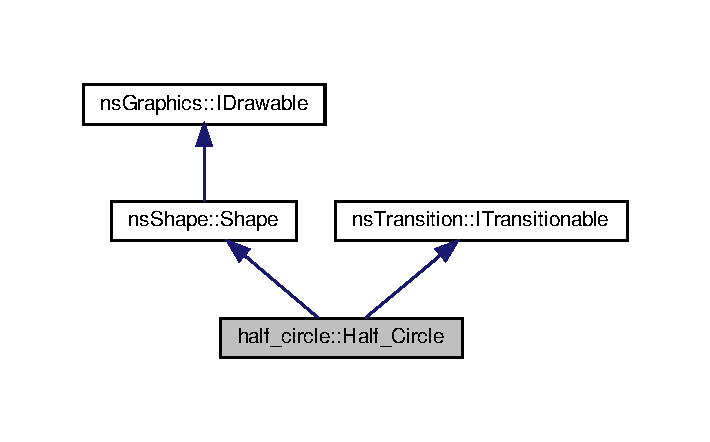
\includegraphics[width=341pt]{classhalf__circle_1_1_half___circle__inherit__graph}
\end{center}
\end{figure}


Collaboration diagram for half\+\_\+circle\+:\+:Half\+\_\+\+Circle\+:
\nopagebreak
\begin{figure}[H]
\begin{center}
\leavevmode
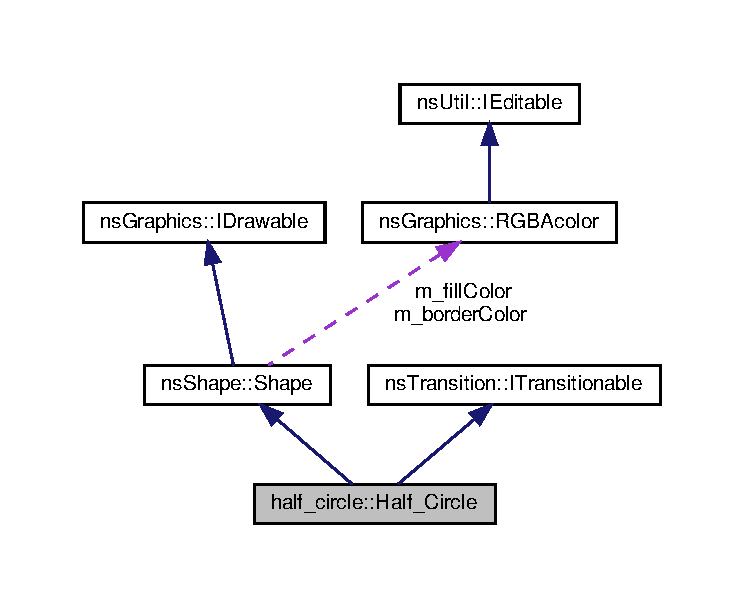
\includegraphics[width=350pt]{classhalf__circle_1_1_half___circle__coll__graph}
\end{center}
\end{figure}
\subsection*{Public Types}
\begin{DoxyCompactItemize}
\item 
enum \hyperlink{classhalf__circle_1_1_half___circle_a7e20290d766bda444243c1c524479304}{Transition\+Ids} \{ \newline
\hyperlink{classhalf__circle_1_1_half___circle_a7e20290d766bda444243c1c524479304ac1e74032d1426ae596f4d6e7525ce0d2}{T\+R\+A\+N\+S\+I\+T\+I\+O\+N\+\_\+\+F\+I\+L\+L\+\_\+\+C\+O\+L\+O\+R\+\_\+\+R\+GB}, 
\hyperlink{classhalf__circle_1_1_half___circle_a7e20290d766bda444243c1c524479304a914039a7453a5ba46ce8e9691f973565}{T\+R\+A\+N\+S\+I\+T\+I\+O\+N\+\_\+\+F\+I\+L\+L\+\_\+\+C\+O\+L\+O\+R\+\_\+\+A\+L\+P\+HA}, 
\hyperlink{classhalf__circle_1_1_half___circle_a7e20290d766bda444243c1c524479304a2a63985872b8198ae91571096266901f}{T\+R\+A\+N\+S\+I\+T\+I\+O\+N\+\_\+\+B\+O\+R\+D\+E\+R\+\_\+\+C\+O\+L\+O\+R\+\_\+\+R\+GB}, 
\hyperlink{classhalf__circle_1_1_half___circle_a7e20290d766bda444243c1c524479304afb901c98dd9e94baa5848287cfd66caf}{T\+R\+A\+N\+S\+I\+T\+I\+O\+N\+\_\+\+B\+O\+R\+D\+E\+R\+\_\+\+C\+O\+L\+O\+R\+\_\+\+A\+L\+P\+HA}, 
\newline
\hyperlink{classhalf__circle_1_1_half___circle_a7e20290d766bda444243c1c524479304ad66fd6a8d99dc4dee199bf18256f4686}{T\+R\+A\+N\+S\+I\+T\+I\+O\+N\+\_\+\+P\+O\+S\+I\+T\+I\+ON}, 
\hyperlink{classhalf__circle_1_1_half___circle_a7e20290d766bda444243c1c524479304a35e42ad23744d956dfe07c03a05ccef7}{T\+R\+A\+N\+S\+I\+T\+I\+O\+N\+\_\+\+R\+A\+D\+I\+US}
 \}\begin{DoxyCompactList}\small\item\em Transition\+Ids \+: Liste de toutes les transitions que cet élément peut exécuter. \end{DoxyCompactList}
\end{DoxyCompactItemize}
\subsection*{Public Member Functions}
\begin{DoxyCompactItemize}
\item 
\hyperlink{classhalf__circle_1_1_half___circle_a4745acf1a6bd730b7272d3deb1d45a10}{Half\+\_\+\+Circle} (const \hyperlink{classns_graphics_1_1_vec2_d}{ns\+Graphics\+::\+Vec2D} \&position, const unsigned \&radius, const unsigned \&height, const char \&direction, const \hyperlink{classns_graphics_1_1_r_g_b_acolor}{ns\+Graphics\+::\+R\+G\+B\+Acolor} \&fill\+Color, const \hyperlink{classns_graphics_1_1_r_g_b_acolor}{ns\+Graphics\+::\+R\+G\+B\+Acolor} \&border\+Color=\hyperlink{namespacens_graphics_ab2001ad03cceb2565849e04465618c1e}{ns\+Graphics\+::\+K\+Transparent})
\begin{DoxyCompactList}\small\item\em Constructeur pour la classe \hyperlink{classhalf__circle_1_1_half___circle}{Half\+\_\+\+Circle}. \end{DoxyCompactList}\item 
virtual \hyperlink{classhalf__circle_1_1_half___circle_a72930c6bddc0f5bb504759a189bb7409}{$\sim$\+Half\+\_\+\+Circle} () override=default
\begin{DoxyCompactList}\small\item\em Destructeur virtuel pour la classe \hyperlink{classhalf__circle_1_1_half___circle}{Half\+\_\+\+Circle}. \end{DoxyCompactList}\item 
virtual void \hyperlink{classhalf__circle_1_1_half___circle_a46b2ea1d78fcacdf2b79707c6431774b}{draw} (\hyperlink{class_min_g_l}{Min\+GL} \&window) const override
\begin{DoxyCompactList}\small\item\em Fonction pour afficher l\textquotesingle{}objet. \end{DoxyCompactList}\item 
virtual void \hyperlink{classhalf__circle_1_1_half___circle_a32fbc3cf8c53b5a239c56b0be6df3e7e}{get\+Values} (const int \&id, std\+::vector$<$ float $>$ \&values) override
\begin{DoxyCompactList}\small\item\em Récupère des valeurs dans un vecteur de float pour l\textquotesingle{}ID spécifié \end{DoxyCompactList}\item 
virtual void \hyperlink{classhalf__circle_1_1_half___circle_ab128d56c2d348524d88da23b89bf3d35}{set\+Values} (const int \&id, const std\+::vector$<$ float $>$ \&values) override
\begin{DoxyCompactList}\small\item\em Définit les nouvelles valeurs pour l\textquotesingle{}ID spécifié \end{DoxyCompactList}\item 
\hyperlink{classhalf__circle_1_1_half___circle}{Half\+\_\+\+Circle} \hyperlink{classhalf__circle_1_1_half___circle_aad1321266f1c80f93426c7b0f906700b}{operator+} (const \hyperlink{classns_graphics_1_1_vec2_d}{ns\+Graphics\+::\+Vec2D} \&\hyperlink{classhalf__circle_1_1_half___circle_abf7d74a747e38464e7897a4e1c54caad}{get\+Position}) const
\begin{DoxyCompactList}\small\item\em Opérateur de décalage. \end{DoxyCompactList}\item 
\hyperlink{classhalf__circle_1_1_half___circle}{Half\+\_\+\+Circle} \hyperlink{classhalf__circle_1_1_half___circle_a378f3ccdfd80602eef6123812aa6281e}{operator$\ast$} (const float \&f) const
\begin{DoxyCompactList}\small\item\em Opérateur de réduction. \end{DoxyCompactList}\item 
const \hyperlink{classns_graphics_1_1_vec2_d}{ns\+Graphics\+::\+Vec2D} \& \hyperlink{classhalf__circle_1_1_half___circle_abf7d74a747e38464e7897a4e1c54caad}{get\+Position} () const
\begin{DoxyCompactList}\small\item\em Récupère la position du demi-\/cercle. \end{DoxyCompactList}\item 
void \hyperlink{classhalf__circle_1_1_half___circle_aef4c8e9f8a7d86c0062511ee24646afa}{set\+Position} (const \hyperlink{classns_graphics_1_1_vec2_d}{ns\+Graphics\+::\+Vec2D} \&position)
\begin{DoxyCompactList}\small\item\em Définit la nouvelle position du demi-\/cercle. \end{DoxyCompactList}\item 
unsigned \hyperlink{classhalf__circle_1_1_half___circle_a528419d14294a981dbc6cfde14c198fe}{get\+Radius} () const
\begin{DoxyCompactList}\small\item\em Récupère le rayon du cercle. \end{DoxyCompactList}\item 
void \hyperlink{classhalf__circle_1_1_half___circle_a84af21356a58484b2de1702e64c162dd}{set\+Radius} (const unsigned \&radius)
\begin{DoxyCompactList}\small\item\em Définit le nouveau rayon du demi-\/cercle. \end{DoxyCompactList}\end{DoxyCompactItemize}
\subsection*{Additional Inherited Members}


\subsection{Detailed Description}
Classe représentant un demi-\/cercle. 

Definition at line 24 of file half\+\_\+circle.\+h.



\subsection{Member Enumeration Documentation}
\mbox{\Hypertarget{classhalf__circle_1_1_half___circle_a7e20290d766bda444243c1c524479304}\label{classhalf__circle_1_1_half___circle_a7e20290d766bda444243c1c524479304}} 
\index{half\+\_\+circle\+::\+Half\+\_\+\+Circle@{half\+\_\+circle\+::\+Half\+\_\+\+Circle}!Transition\+Ids@{Transition\+Ids}}
\index{Transition\+Ids@{Transition\+Ids}!half\+\_\+circle\+::\+Half\+\_\+\+Circle@{half\+\_\+circle\+::\+Half\+\_\+\+Circle}}
\subsubsection{\texorpdfstring{Transition\+Ids}{TransitionIds}}
{\footnotesize\ttfamily enum \hyperlink{classhalf__circle_1_1_half___circle_a7e20290d766bda444243c1c524479304}{half\+\_\+circle\+::\+Half\+\_\+\+Circle\+::\+Transition\+Ids}}



Transition\+Ids \+: Liste de toutes les transitions que cet élément peut exécuter. 

\begin{DoxyEnumFields}{Enumerator}
\raisebox{\heightof{T}}[0pt][0pt]{\index{T\+R\+A\+N\+S\+I\+T\+I\+O\+N\+\_\+\+F\+I\+L\+L\+\_\+\+C\+O\+L\+O\+R\+\_\+\+R\+GB@{T\+R\+A\+N\+S\+I\+T\+I\+O\+N\+\_\+\+F\+I\+L\+L\+\_\+\+C\+O\+L\+O\+R\+\_\+\+R\+GB}!half\+\_\+circle\+::\+Half\+\_\+\+Circle@{half\+\_\+circle\+::\+Half\+\_\+\+Circle}}\index{half\+\_\+circle\+::\+Half\+\_\+\+Circle@{half\+\_\+circle\+::\+Half\+\_\+\+Circle}!T\+R\+A\+N\+S\+I\+T\+I\+O\+N\+\_\+\+F\+I\+L\+L\+\_\+\+C\+O\+L\+O\+R\+\_\+\+R\+GB@{T\+R\+A\+N\+S\+I\+T\+I\+O\+N\+\_\+\+F\+I\+L\+L\+\_\+\+C\+O\+L\+O\+R\+\_\+\+R\+GB}}}\mbox{\Hypertarget{classhalf__circle_1_1_half___circle_a7e20290d766bda444243c1c524479304ac1e74032d1426ae596f4d6e7525ce0d2}\label{classhalf__circle_1_1_half___circle_a7e20290d766bda444243c1c524479304ac1e74032d1426ae596f4d6e7525ce0d2}} 
T\+R\+A\+N\+S\+I\+T\+I\+O\+N\+\_\+\+F\+I\+L\+L\+\_\+\+C\+O\+L\+O\+R\+\_\+\+R\+GB&Transition pour la couleur de remplissage \\
\hline

\raisebox{\heightof{T}}[0pt][0pt]{\index{T\+R\+A\+N\+S\+I\+T\+I\+O\+N\+\_\+\+F\+I\+L\+L\+\_\+\+C\+O\+L\+O\+R\+\_\+\+A\+L\+P\+HA@{T\+R\+A\+N\+S\+I\+T\+I\+O\+N\+\_\+\+F\+I\+L\+L\+\_\+\+C\+O\+L\+O\+R\+\_\+\+A\+L\+P\+HA}!half\+\_\+circle\+::\+Half\+\_\+\+Circle@{half\+\_\+circle\+::\+Half\+\_\+\+Circle}}\index{half\+\_\+circle\+::\+Half\+\_\+\+Circle@{half\+\_\+circle\+::\+Half\+\_\+\+Circle}!T\+R\+A\+N\+S\+I\+T\+I\+O\+N\+\_\+\+F\+I\+L\+L\+\_\+\+C\+O\+L\+O\+R\+\_\+\+A\+L\+P\+HA@{T\+R\+A\+N\+S\+I\+T\+I\+O\+N\+\_\+\+F\+I\+L\+L\+\_\+\+C\+O\+L\+O\+R\+\_\+\+A\+L\+P\+HA}}}\mbox{\Hypertarget{classhalf__circle_1_1_half___circle_a7e20290d766bda444243c1c524479304a914039a7453a5ba46ce8e9691f973565}\label{classhalf__circle_1_1_half___circle_a7e20290d766bda444243c1c524479304a914039a7453a5ba46ce8e9691f973565}} 
T\+R\+A\+N\+S\+I\+T\+I\+O\+N\+\_\+\+F\+I\+L\+L\+\_\+\+C\+O\+L\+O\+R\+\_\+\+A\+L\+P\+HA&Transition pour la transparence de remplissage \\
\hline

\raisebox{\heightof{T}}[0pt][0pt]{\index{T\+R\+A\+N\+S\+I\+T\+I\+O\+N\+\_\+\+B\+O\+R\+D\+E\+R\+\_\+\+C\+O\+L\+O\+R\+\_\+\+R\+GB@{T\+R\+A\+N\+S\+I\+T\+I\+O\+N\+\_\+\+B\+O\+R\+D\+E\+R\+\_\+\+C\+O\+L\+O\+R\+\_\+\+R\+GB}!half\+\_\+circle\+::\+Half\+\_\+\+Circle@{half\+\_\+circle\+::\+Half\+\_\+\+Circle}}\index{half\+\_\+circle\+::\+Half\+\_\+\+Circle@{half\+\_\+circle\+::\+Half\+\_\+\+Circle}!T\+R\+A\+N\+S\+I\+T\+I\+O\+N\+\_\+\+B\+O\+R\+D\+E\+R\+\_\+\+C\+O\+L\+O\+R\+\_\+\+R\+GB@{T\+R\+A\+N\+S\+I\+T\+I\+O\+N\+\_\+\+B\+O\+R\+D\+E\+R\+\_\+\+C\+O\+L\+O\+R\+\_\+\+R\+GB}}}\mbox{\Hypertarget{classhalf__circle_1_1_half___circle_a7e20290d766bda444243c1c524479304a2a63985872b8198ae91571096266901f}\label{classhalf__circle_1_1_half___circle_a7e20290d766bda444243c1c524479304a2a63985872b8198ae91571096266901f}} 
T\+R\+A\+N\+S\+I\+T\+I\+O\+N\+\_\+\+B\+O\+R\+D\+E\+R\+\_\+\+C\+O\+L\+O\+R\+\_\+\+R\+GB&Transition pour la couleur de bord \\
\hline

\raisebox{\heightof{T}}[0pt][0pt]{\index{T\+R\+A\+N\+S\+I\+T\+I\+O\+N\+\_\+\+B\+O\+R\+D\+E\+R\+\_\+\+C\+O\+L\+O\+R\+\_\+\+A\+L\+P\+HA@{T\+R\+A\+N\+S\+I\+T\+I\+O\+N\+\_\+\+B\+O\+R\+D\+E\+R\+\_\+\+C\+O\+L\+O\+R\+\_\+\+A\+L\+P\+HA}!half\+\_\+circle\+::\+Half\+\_\+\+Circle@{half\+\_\+circle\+::\+Half\+\_\+\+Circle}}\index{half\+\_\+circle\+::\+Half\+\_\+\+Circle@{half\+\_\+circle\+::\+Half\+\_\+\+Circle}!T\+R\+A\+N\+S\+I\+T\+I\+O\+N\+\_\+\+B\+O\+R\+D\+E\+R\+\_\+\+C\+O\+L\+O\+R\+\_\+\+A\+L\+P\+HA@{T\+R\+A\+N\+S\+I\+T\+I\+O\+N\+\_\+\+B\+O\+R\+D\+E\+R\+\_\+\+C\+O\+L\+O\+R\+\_\+\+A\+L\+P\+HA}}}\mbox{\Hypertarget{classhalf__circle_1_1_half___circle_a7e20290d766bda444243c1c524479304afb901c98dd9e94baa5848287cfd66caf}\label{classhalf__circle_1_1_half___circle_a7e20290d766bda444243c1c524479304afb901c98dd9e94baa5848287cfd66caf}} 
T\+R\+A\+N\+S\+I\+T\+I\+O\+N\+\_\+\+B\+O\+R\+D\+E\+R\+\_\+\+C\+O\+L\+O\+R\+\_\+\+A\+L\+P\+HA&Transition pour la transparence de bord \\
\hline

\raisebox{\heightof{T}}[0pt][0pt]{\index{T\+R\+A\+N\+S\+I\+T\+I\+O\+N\+\_\+\+P\+O\+S\+I\+T\+I\+ON@{T\+R\+A\+N\+S\+I\+T\+I\+O\+N\+\_\+\+P\+O\+S\+I\+T\+I\+ON}!half\+\_\+circle\+::\+Half\+\_\+\+Circle@{half\+\_\+circle\+::\+Half\+\_\+\+Circle}}\index{half\+\_\+circle\+::\+Half\+\_\+\+Circle@{half\+\_\+circle\+::\+Half\+\_\+\+Circle}!T\+R\+A\+N\+S\+I\+T\+I\+O\+N\+\_\+\+P\+O\+S\+I\+T\+I\+ON@{T\+R\+A\+N\+S\+I\+T\+I\+O\+N\+\_\+\+P\+O\+S\+I\+T\+I\+ON}}}\mbox{\Hypertarget{classhalf__circle_1_1_half___circle_a7e20290d766bda444243c1c524479304ad66fd6a8d99dc4dee199bf18256f4686}\label{classhalf__circle_1_1_half___circle_a7e20290d766bda444243c1c524479304ad66fd6a8d99dc4dee199bf18256f4686}} 
T\+R\+A\+N\+S\+I\+T\+I\+O\+N\+\_\+\+P\+O\+S\+I\+T\+I\+ON&Transition pour la position \\
\hline

\raisebox{\heightof{T}}[0pt][0pt]{\index{T\+R\+A\+N\+S\+I\+T\+I\+O\+N\+\_\+\+R\+A\+D\+I\+US@{T\+R\+A\+N\+S\+I\+T\+I\+O\+N\+\_\+\+R\+A\+D\+I\+US}!half\+\_\+circle\+::\+Half\+\_\+\+Circle@{half\+\_\+circle\+::\+Half\+\_\+\+Circle}}\index{half\+\_\+circle\+::\+Half\+\_\+\+Circle@{half\+\_\+circle\+::\+Half\+\_\+\+Circle}!T\+R\+A\+N\+S\+I\+T\+I\+O\+N\+\_\+\+R\+A\+D\+I\+US@{T\+R\+A\+N\+S\+I\+T\+I\+O\+N\+\_\+\+R\+A\+D\+I\+US}}}\mbox{\Hypertarget{classhalf__circle_1_1_half___circle_a7e20290d766bda444243c1c524479304a35e42ad23744d956dfe07c03a05ccef7}\label{classhalf__circle_1_1_half___circle_a7e20290d766bda444243c1c524479304a35e42ad23744d956dfe07c03a05ccef7}} 
T\+R\+A\+N\+S\+I\+T\+I\+O\+N\+\_\+\+R\+A\+D\+I\+US&Transition pour le rayon \\
\hline

\end{DoxyEnumFields}


Definition at line 30 of file half\+\_\+circle.\+h.



\subsection{Constructor \& Destructor Documentation}
\mbox{\Hypertarget{classhalf__circle_1_1_half___circle_a4745acf1a6bd730b7272d3deb1d45a10}\label{classhalf__circle_1_1_half___circle_a4745acf1a6bd730b7272d3deb1d45a10}} 
\index{half\+\_\+circle\+::\+Half\+\_\+\+Circle@{half\+\_\+circle\+::\+Half\+\_\+\+Circle}!Half\+\_\+\+Circle@{Half\+\_\+\+Circle}}
\index{Half\+\_\+\+Circle@{Half\+\_\+\+Circle}!half\+\_\+circle\+::\+Half\+\_\+\+Circle@{half\+\_\+circle\+::\+Half\+\_\+\+Circle}}
\subsubsection{\texorpdfstring{Half\+\_\+\+Circle()}{Half\_Circle()}}
{\footnotesize\ttfamily half\+\_\+circle\+::\+Half\+\_\+\+Circle\+::\+Half\+\_\+\+Circle (\begin{DoxyParamCaption}\item[{const \hyperlink{classns_graphics_1_1_vec2_d}{ns\+Graphics\+::\+Vec2D} \&}]{position,  }\item[{const unsigned \&}]{radius,  }\item[{const unsigned \&}]{height,  }\item[{const char \&}]{direction,  }\item[{const \hyperlink{classns_graphics_1_1_r_g_b_acolor}{ns\+Graphics\+::\+R\+G\+B\+Acolor} \&}]{fill\+Color,  }\item[{const \hyperlink{classns_graphics_1_1_r_g_b_acolor}{ns\+Graphics\+::\+R\+G\+B\+Acolor} \&}]{border\+Color = {\ttfamily \hyperlink{namespacens_graphics_ab2001ad03cceb2565849e04465618c1e}{ns\+Graphics\+::\+K\+Transparent}} }\end{DoxyParamCaption})}



Constructeur pour la classe \hyperlink{classhalf__circle_1_1_half___circle}{Half\+\_\+\+Circle}. 


\begin{DoxyParams}[1]{Parameters}
\mbox{\tt in}  & {\em position} & \+: Position du centre \\
\hline
\mbox{\tt in}  & {\em radius} & \+: Rayon du demi-\/cercle \\
\hline
\mbox{\tt in}  & {\em height} & Hauteur du demi-\/cercle \\
\hline
\mbox{\tt in}  & {\em direction} & \+: Direction du demi-\/cercle \\
\hline
\mbox{\tt in}  & {\em fill\+Color} & \+: Couleur de remplissage \\
\hline
\mbox{\tt in}  & {\em border\+Color} & \+: Couleur de bord \\
\hline
\end{DoxyParams}


Definition at line 25 of file half\+\_\+circle.\+cpp.

\mbox{\Hypertarget{classhalf__circle_1_1_half___circle_a72930c6bddc0f5bb504759a189bb7409}\label{classhalf__circle_1_1_half___circle_a72930c6bddc0f5bb504759a189bb7409}} 
\index{half\+\_\+circle\+::\+Half\+\_\+\+Circle@{half\+\_\+circle\+::\+Half\+\_\+\+Circle}!````~Half\+\_\+\+Circle@{$\sim$\+Half\+\_\+\+Circle}}
\index{````~Half\+\_\+\+Circle@{$\sim$\+Half\+\_\+\+Circle}!half\+\_\+circle\+::\+Half\+\_\+\+Circle@{half\+\_\+circle\+::\+Half\+\_\+\+Circle}}
\subsubsection{\texorpdfstring{$\sim$\+Half\+\_\+\+Circle()}{~Half\_Circle()}}
{\footnotesize\ttfamily half\+\_\+circle\+::\+Half\+\_\+\+Circle\+::$\sim$\+Half\+\_\+\+Circle (\begin{DoxyParamCaption}{ }\end{DoxyParamCaption})\hspace{0.3cm}{\ttfamily [override]}, {\ttfamily [virtual]}, {\ttfamily [default]}}



Destructeur virtuel pour la classe \hyperlink{classhalf__circle_1_1_half___circle}{Half\+\_\+\+Circle}. 



\subsection{Member Function Documentation}
\mbox{\Hypertarget{classhalf__circle_1_1_half___circle_a46b2ea1d78fcacdf2b79707c6431774b}\label{classhalf__circle_1_1_half___circle_a46b2ea1d78fcacdf2b79707c6431774b}} 
\index{half\+\_\+circle\+::\+Half\+\_\+\+Circle@{half\+\_\+circle\+::\+Half\+\_\+\+Circle}!draw@{draw}}
\index{draw@{draw}!half\+\_\+circle\+::\+Half\+\_\+\+Circle@{half\+\_\+circle\+::\+Half\+\_\+\+Circle}}
\subsubsection{\texorpdfstring{draw()}{draw()}}
{\footnotesize\ttfamily void half\+\_\+circle\+::\+Half\+\_\+\+Circle\+::draw (\begin{DoxyParamCaption}\item[{\hyperlink{class_min_g_l}{Min\+GL} \&}]{window }\end{DoxyParamCaption}) const\hspace{0.3cm}{\ttfamily [override]}, {\ttfamily [virtual]}}



Fonction pour afficher l\textquotesingle{}objet. 



Implements \hyperlink{classns_graphics_1_1_i_drawable_abed8a61e1d507d31e76f0891f3bf9c51}{ns\+Graphics\+::\+I\+Drawable}.



Definition at line 33 of file half\+\_\+circle.\+cpp.

\mbox{\Hypertarget{classhalf__circle_1_1_half___circle_abf7d74a747e38464e7897a4e1c54caad}\label{classhalf__circle_1_1_half___circle_abf7d74a747e38464e7897a4e1c54caad}} 
\index{half\+\_\+circle\+::\+Half\+\_\+\+Circle@{half\+\_\+circle\+::\+Half\+\_\+\+Circle}!get\+Position@{get\+Position}}
\index{get\+Position@{get\+Position}!half\+\_\+circle\+::\+Half\+\_\+\+Circle@{half\+\_\+circle\+::\+Half\+\_\+\+Circle}}
\subsubsection{\texorpdfstring{get\+Position()}{getPosition()}}
{\footnotesize\ttfamily const \hyperlink{classns_graphics_1_1_vec2_d}{ns\+Graphics\+::\+Vec2D} \& half\+\_\+circle\+::\+Half\+\_\+\+Circle\+::get\+Position (\begin{DoxyParamCaption}{ }\end{DoxyParamCaption}) const}



Récupère la position du demi-\/cercle. 

\mbox{\Hypertarget{classhalf__circle_1_1_half___circle_a528419d14294a981dbc6cfde14c198fe}\label{classhalf__circle_1_1_half___circle_a528419d14294a981dbc6cfde14c198fe}} 
\index{half\+\_\+circle\+::\+Half\+\_\+\+Circle@{half\+\_\+circle\+::\+Half\+\_\+\+Circle}!get\+Radius@{get\+Radius}}
\index{get\+Radius@{get\+Radius}!half\+\_\+circle\+::\+Half\+\_\+\+Circle@{half\+\_\+circle\+::\+Half\+\_\+\+Circle}}
\subsubsection{\texorpdfstring{get\+Radius()}{getRadius()}}
{\footnotesize\ttfamily unsigned half\+\_\+circle\+::\+Half\+\_\+\+Circle\+::get\+Radius (\begin{DoxyParamCaption}{ }\end{DoxyParamCaption}) const}



Récupère le rayon du cercle. 

\mbox{\Hypertarget{classhalf__circle_1_1_half___circle_a32fbc3cf8c53b5a239c56b0be6df3e7e}\label{classhalf__circle_1_1_half___circle_a32fbc3cf8c53b5a239c56b0be6df3e7e}} 
\index{half\+\_\+circle\+::\+Half\+\_\+\+Circle@{half\+\_\+circle\+::\+Half\+\_\+\+Circle}!get\+Values@{get\+Values}}
\index{get\+Values@{get\+Values}!half\+\_\+circle\+::\+Half\+\_\+\+Circle@{half\+\_\+circle\+::\+Half\+\_\+\+Circle}}
\subsubsection{\texorpdfstring{get\+Values()}{getValues()}}
{\footnotesize\ttfamily void half\+\_\+circle\+::\+Half\+\_\+\+Circle\+::get\+Values (\begin{DoxyParamCaption}\item[{const int \&}]{id,  }\item[{std\+::vector$<$ float $>$ \&}]{values }\end{DoxyParamCaption})\hspace{0.3cm}{\ttfamily [override]}, {\ttfamily [virtual]}}



Récupère des valeurs dans un vecteur de float pour l\textquotesingle{}ID spécifié 


\begin{DoxyParams}[1]{Parameters}
\mbox{\tt in}  & {\em id} & ID des valeurs a récupérer \\
\hline
\mbox{\tt in,out}  & {\em values} & Vecteur de valeurs a peupler \\
\hline
\end{DoxyParams}


Implements \hyperlink{classns_transition_1_1_i_transitionable_a5871a16fd47c1e5c8bacdd5da8597ed9}{ns\+Transition\+::\+I\+Transitionable}.



Definition at line 81 of file half\+\_\+circle.\+cpp.

\mbox{\Hypertarget{classhalf__circle_1_1_half___circle_a378f3ccdfd80602eef6123812aa6281e}\label{classhalf__circle_1_1_half___circle_a378f3ccdfd80602eef6123812aa6281e}} 
\index{half\+\_\+circle\+::\+Half\+\_\+\+Circle@{half\+\_\+circle\+::\+Half\+\_\+\+Circle}!operator$\ast$@{operator$\ast$}}
\index{operator$\ast$@{operator$\ast$}!half\+\_\+circle\+::\+Half\+\_\+\+Circle@{half\+\_\+circle\+::\+Half\+\_\+\+Circle}}
\subsubsection{\texorpdfstring{operator$\ast$()}{operator*()}}
{\footnotesize\ttfamily \hyperlink{classhalf__circle_1_1_half___circle}{Half\+\_\+\+Circle} half\+\_\+circle\+::\+Half\+\_\+\+Circle\+::operator$\ast$ (\begin{DoxyParamCaption}\item[{const float \&}]{f }\end{DoxyParamCaption}) const}



Opérateur de réduction. 


\begin{DoxyParams}[1]{Parameters}
\mbox{\tt in}  & {\em f} & \+: Nombre avec lequel multiplier la position actuelle \\
\hline
\end{DoxyParams}
\mbox{\Hypertarget{classhalf__circle_1_1_half___circle_aad1321266f1c80f93426c7b0f906700b}\label{classhalf__circle_1_1_half___circle_aad1321266f1c80f93426c7b0f906700b}} 
\index{half\+\_\+circle\+::\+Half\+\_\+\+Circle@{half\+\_\+circle\+::\+Half\+\_\+\+Circle}!operator+@{operator+}}
\index{operator+@{operator+}!half\+\_\+circle\+::\+Half\+\_\+\+Circle@{half\+\_\+circle\+::\+Half\+\_\+\+Circle}}
\subsubsection{\texorpdfstring{operator+()}{operator+()}}
{\footnotesize\ttfamily \hyperlink{classhalf__circle_1_1_half___circle}{Half\+\_\+\+Circle} half\+\_\+circle\+::\+Half\+\_\+\+Circle\+::operator+ (\begin{DoxyParamCaption}\item[{const \hyperlink{classns_graphics_1_1_vec2_d}{ns\+Graphics\+::\+Vec2D} \&}]{position }\end{DoxyParamCaption}) const}



Opérateur de décalage. 


\begin{DoxyParams}[1]{Parameters}
\mbox{\tt in}  & {\em position} & \+: Position a additionner \\
\hline
\end{DoxyParams}
\mbox{\Hypertarget{classhalf__circle_1_1_half___circle_aef4c8e9f8a7d86c0062511ee24646afa}\label{classhalf__circle_1_1_half___circle_aef4c8e9f8a7d86c0062511ee24646afa}} 
\index{half\+\_\+circle\+::\+Half\+\_\+\+Circle@{half\+\_\+circle\+::\+Half\+\_\+\+Circle}!set\+Position@{set\+Position}}
\index{set\+Position@{set\+Position}!half\+\_\+circle\+::\+Half\+\_\+\+Circle@{half\+\_\+circle\+::\+Half\+\_\+\+Circle}}
\subsubsection{\texorpdfstring{set\+Position()}{setPosition()}}
{\footnotesize\ttfamily void half\+\_\+circle\+::\+Half\+\_\+\+Circle\+::set\+Position (\begin{DoxyParamCaption}\item[{const \hyperlink{classns_graphics_1_1_vec2_d}{ns\+Graphics\+::\+Vec2D} \&}]{position }\end{DoxyParamCaption})}



Définit la nouvelle position du demi-\/cercle. 


\begin{DoxyParams}[1]{Parameters}
\mbox{\tt in}  & {\em position} & \+: Nouvelle position \\
\hline
\end{DoxyParams}
\mbox{\Hypertarget{classhalf__circle_1_1_half___circle_a84af21356a58484b2de1702e64c162dd}\label{classhalf__circle_1_1_half___circle_a84af21356a58484b2de1702e64c162dd}} 
\index{half\+\_\+circle\+::\+Half\+\_\+\+Circle@{half\+\_\+circle\+::\+Half\+\_\+\+Circle}!set\+Radius@{set\+Radius}}
\index{set\+Radius@{set\+Radius}!half\+\_\+circle\+::\+Half\+\_\+\+Circle@{half\+\_\+circle\+::\+Half\+\_\+\+Circle}}
\subsubsection{\texorpdfstring{set\+Radius()}{setRadius()}}
{\footnotesize\ttfamily half\+\_\+circle\+::\+Half\+\_\+\+Circle\+::set\+Radius (\begin{DoxyParamCaption}\item[{const unsigned \&}]{radius }\end{DoxyParamCaption})}



Définit le nouveau rayon du demi-\/cercle. 


\begin{DoxyParams}[1]{Parameters}
\mbox{\tt in}  & {\em radius} & \+: Nouveau rayon \\
\hline
\end{DoxyParams}
\mbox{\Hypertarget{classhalf__circle_1_1_half___circle_ab128d56c2d348524d88da23b89bf3d35}\label{classhalf__circle_1_1_half___circle_ab128d56c2d348524d88da23b89bf3d35}} 
\index{half\+\_\+circle\+::\+Half\+\_\+\+Circle@{half\+\_\+circle\+::\+Half\+\_\+\+Circle}!set\+Values@{set\+Values}}
\index{set\+Values@{set\+Values}!half\+\_\+circle\+::\+Half\+\_\+\+Circle@{half\+\_\+circle\+::\+Half\+\_\+\+Circle}}
\subsubsection{\texorpdfstring{set\+Values()}{setValues()}}
{\footnotesize\ttfamily void half\+\_\+circle\+::\+Half\+\_\+\+Circle\+::set\+Values (\begin{DoxyParamCaption}\item[{const int \&}]{id,  }\item[{const std\+::vector$<$ float $>$ \&}]{values }\end{DoxyParamCaption})\hspace{0.3cm}{\ttfamily [override]}, {\ttfamily [virtual]}}



Définit les nouvelles valeurs pour l\textquotesingle{}ID spécifié 


\begin{DoxyParams}[1]{Parameters}
\mbox{\tt in}  & {\em id} & ID des valeurs a définir \\
\hline
\mbox{\tt in}  & {\em values} & Vecteur des nouvelles valeurs a appliquer \\
\hline
\end{DoxyParams}


Implements \hyperlink{classns_transition_1_1_i_transitionable_ade37d29f7f2ca4890ed0e2e64d033197}{ns\+Transition\+::\+I\+Transitionable}.



Definition at line 121 of file half\+\_\+circle.\+cpp.



The documentation for this class was generated from the following files\+:\begin{DoxyCompactItemize}
\item 
libs/game/graphic/\hyperlink{half__circle_8h}{half\+\_\+circle.\+h}\item 
src/graphic/\hyperlink{half__circle_8cpp}{half\+\_\+circle.\+cpp}\end{DoxyCompactItemize}

\hypertarget{classns_graphics_1_1_i_drawable}{}\section{ns\+Graphics\+:\+:I\+Drawable Class Reference}
\label{classns_graphics_1_1_i_drawable}\index{ns\+Graphics\+::\+I\+Drawable@{ns\+Graphics\+::\+I\+Drawable}}


Interface pour un objet affichable.  




{\ttfamily \#include $<$idrawable.\+h$>$}



Inheritance diagram for ns\+Graphics\+:\+:I\+Drawable\+:
\nopagebreak
\begin{figure}[H]
\begin{center}
\leavevmode
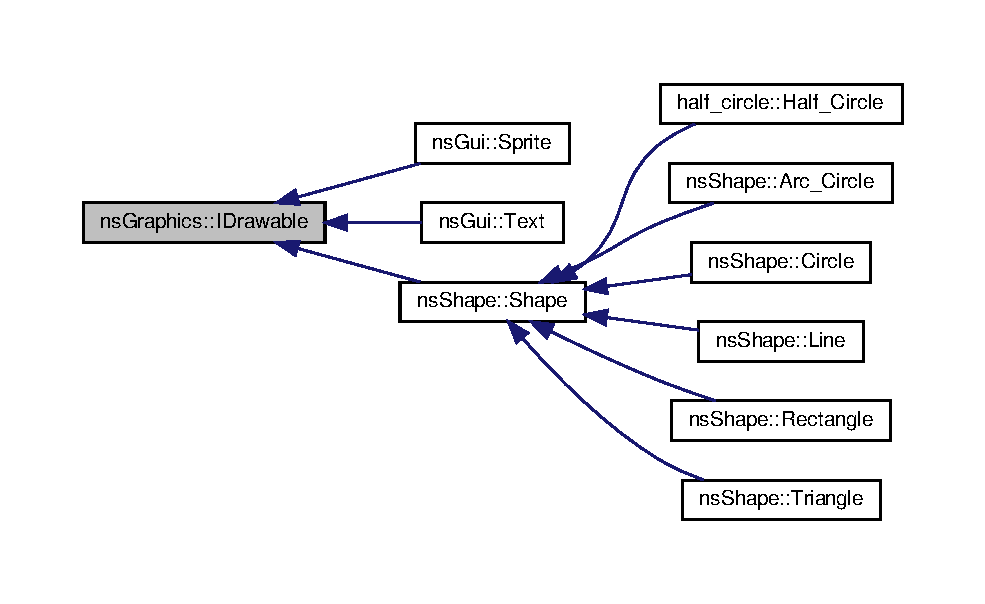
\includegraphics[width=350pt]{classns_graphics_1_1_i_drawable__inherit__graph}
\end{center}
\end{figure}
\subsection*{Public Member Functions}
\begin{DoxyCompactItemize}
\item 
virtual \hyperlink{classns_graphics_1_1_i_drawable_ab7a2ae7682163969bd4627e402ef0867}{$\sim$\+I\+Drawable} ()=default
\begin{DoxyCompactList}\small\item\em Destructeur pour la classe \hyperlink{classns_graphics_1_1_i_drawable}{I\+Drawable}. \end{DoxyCompactList}\item 
virtual void \hyperlink{classns_graphics_1_1_i_drawable_abed8a61e1d507d31e76f0891f3bf9c51}{draw} (\hyperlink{class_min_g_l}{Min\+GL} \&window) const =0
\begin{DoxyCompactList}\small\item\em Fonction pour afficher l\textquotesingle{}objet. \end{DoxyCompactList}\end{DoxyCompactItemize}
\subsection*{Friends}
\begin{DoxyCompactItemize}
\item 
\hyperlink{class_min_g_l}{Min\+GL} \& \hyperlink{classns_graphics_1_1_i_drawable_a9bb3952d4e675a663f2dbbda11e79395}{operator$<$$<$} (\hyperlink{class_min_g_l}{Min\+GL} \&window, const \hyperlink{classns_graphics_1_1_i_drawable}{I\+Drawable} \&drawable)
\begin{DoxyCompactList}\small\item\em Surcharge de l\textquotesingle{}opérateur d\textquotesingle{}injection. \end{DoxyCompactList}\end{DoxyCompactItemize}


\subsection{Detailed Description}
Interface pour un objet affichable. 

Definition at line 29 of file idrawable.\+h.



\subsection{Constructor \& Destructor Documentation}
\mbox{\Hypertarget{classns_graphics_1_1_i_drawable_ab7a2ae7682163969bd4627e402ef0867}\label{classns_graphics_1_1_i_drawable_ab7a2ae7682163969bd4627e402ef0867}} 
\index{ns\+Graphics\+::\+I\+Drawable@{ns\+Graphics\+::\+I\+Drawable}!````~I\+Drawable@{$\sim$\+I\+Drawable}}
\index{````~I\+Drawable@{$\sim$\+I\+Drawable}!ns\+Graphics\+::\+I\+Drawable@{ns\+Graphics\+::\+I\+Drawable}}
\subsubsection{\texorpdfstring{$\sim$\+I\+Drawable()}{~IDrawable()}}
{\footnotesize\ttfamily ns\+Graphics\+::\+I\+Drawable\+::$\sim$\+I\+Drawable (\begin{DoxyParamCaption}{ }\end{DoxyParamCaption})\hspace{0.3cm}{\ttfamily [virtual]}, {\ttfamily [default]}}



Destructeur pour la classe \hyperlink{classns_graphics_1_1_i_drawable}{I\+Drawable}. 



\subsection{Member Function Documentation}
\mbox{\Hypertarget{classns_graphics_1_1_i_drawable_abed8a61e1d507d31e76f0891f3bf9c51}\label{classns_graphics_1_1_i_drawable_abed8a61e1d507d31e76f0891f3bf9c51}} 
\index{ns\+Graphics\+::\+I\+Drawable@{ns\+Graphics\+::\+I\+Drawable}!draw@{draw}}
\index{draw@{draw}!ns\+Graphics\+::\+I\+Drawable@{ns\+Graphics\+::\+I\+Drawable}}
\subsubsection{\texorpdfstring{draw()}{draw()}}
{\footnotesize\ttfamily void ns\+Graphics\+::\+I\+Drawable\+::draw (\begin{DoxyParamCaption}\item[{\hyperlink{class_min_g_l}{Min\+GL} \&}]{window }\end{DoxyParamCaption}) const\hspace{0.3cm}{\ttfamily [pure virtual]}}



Fonction pour afficher l\textquotesingle{}objet. 



Implemented in \hyperlink{classns_gui_1_1_text_ac353893e3b7cce7585c619acbc0e255b}{ns\+Gui\+::\+Text}, \hyperlink{classns_shape_1_1_rectangle_acbe8ed9e23b67090e7638563f2593735}{ns\+Shape\+::\+Rectangle}, \hyperlink{classns_shape_1_1_arc___circle_a1e789ca962aeefd7dfd861eb0f75a6d7}{ns\+Shape\+::\+Arc\+\_\+\+Circle}, \hyperlink{classns_shape_1_1_triangle_a4b3867fb0e15995b2a6c261d9b0d968d}{ns\+Shape\+::\+Triangle}, \hyperlink{classns_shape_1_1_line_ae14d0de306fa91ee38bafd1d27682beb}{ns\+Shape\+::\+Line}, \hyperlink{classhalf__circle_1_1_half___circle_a46b2ea1d78fcacdf2b79707c6431774b}{half\+\_\+circle\+::\+Half\+\_\+\+Circle}, \hyperlink{classns_shape_1_1_circle_a279581f6104719395091039cea1707e5}{ns\+Shape\+::\+Circle}, and \hyperlink{classns_gui_1_1_sprite_a15157c69a1d792080d2b41519659418c}{ns\+Gui\+::\+Sprite}.



\subsection{Friends And Related Function Documentation}
\mbox{\Hypertarget{classns_graphics_1_1_i_drawable_a9bb3952d4e675a663f2dbbda11e79395}\label{classns_graphics_1_1_i_drawable_a9bb3952d4e675a663f2dbbda11e79395}} 
\index{ns\+Graphics\+::\+I\+Drawable@{ns\+Graphics\+::\+I\+Drawable}!operator$<$$<$@{operator$<$$<$}}
\index{operator$<$$<$@{operator$<$$<$}!ns\+Graphics\+::\+I\+Drawable@{ns\+Graphics\+::\+I\+Drawable}}
\subsubsection{\texorpdfstring{operator$<$$<$}{operator<<}}
{\footnotesize\ttfamily \hyperlink{class_min_g_l}{Min\+GL} \& operator$<$$<$ (\begin{DoxyParamCaption}\item[{\hyperlink{class_min_g_l}{Min\+GL} \&}]{window,  }\item[{const \hyperlink{classns_graphics_1_1_i_drawable}{I\+Drawable} \&}]{drawable }\end{DoxyParamCaption})\hspace{0.3cm}{\ttfamily [friend]}}



Surcharge de l\textquotesingle{}opérateur d\textquotesingle{}injection. 


\begin{DoxyParams}[1]{Parameters}
\mbox{\tt in}  & {\em window} & \+: Fenêtre dans laquelle injecter l\textquotesingle{}élément \\
\hline
\mbox{\tt in}  & {\em drawable} & \+: Elément a injecter \\
\hline
\end{DoxyParams}


Definition at line 51 of file idrawable.\+h.



The documentation for this class was generated from the following file\+:\begin{DoxyCompactItemize}
\item 
libs/mingl/graphics/\hyperlink{idrawable_8h}{idrawable.\+h}\end{DoxyCompactItemize}

\hypertarget{classns_util_1_1_i_editable}{}\section{ns\+Util\+:\+:I\+Editable Class Reference}
\label{classns_util_1_1_i_editable}\index{ns\+Util\+::\+I\+Editable@{ns\+Util\+::\+I\+Editable}}


Interface pour un objet injectable.  




{\ttfamily \#include $<$ieditable.\+h$>$}



Inheritance diagram for ns\+Util\+:\+:I\+Editable\+:
\nopagebreak
\begin{figure}[H]
\begin{center}
\leavevmode
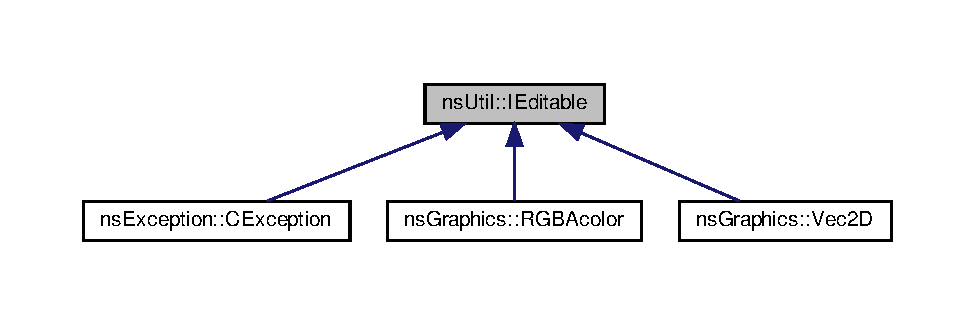
\includegraphics[width=350pt]{classns_util_1_1_i_editable__inherit__graph}
\end{center}
\end{figure}
\subsection*{Public Member Functions}
\begin{DoxyCompactItemize}
\item 
virtual \hyperlink{classns_util_1_1_i_editable_a504b91af8e4efa46357d7236b86b8e2e}{$\sim$\+I\+Editable} ()=default
\begin{DoxyCompactList}\small\item\em Destructeur pour la classe \hyperlink{classns_util_1_1_i_editable}{I\+Editable}. \end{DoxyCompactList}\end{DoxyCompactItemize}
\subsection*{Protected Member Functions}
\begin{DoxyCompactItemize}
\item 
virtual std\+::ostream \& \hyperlink{classns_util_1_1_i_editable_ab20bbe582b95383ed3f1453109035853}{\+\_\+\+Edit} (std\+::ostream \&os) const =0
\begin{DoxyCompactList}\small\item\em Fonction appelée pour injecter l\textquotesingle{}objet courant dans un flux. \end{DoxyCompactList}\end{DoxyCompactItemize}
\subsection*{Friends}
\begin{DoxyCompactItemize}
\item 
std\+::ostream \& \hyperlink{classns_util_1_1_i_editable_a53db4e7832b7c4579b331800bb0cae70}{operator$<$$<$} (std\+::ostream \&os, const \hyperlink{classns_util_1_1_i_editable}{I\+Editable} \&Obj)
\begin{DoxyCompactList}\small\item\em Surcharge de l\textquotesingle{}opérateur d\textquotesingle{}injection. \end{DoxyCompactList}\end{DoxyCompactItemize}


\subsection{Detailed Description}
Interface pour un objet injectable. 

Definition at line 37 of file ieditable.\+h.



\subsection{Constructor \& Destructor Documentation}
\mbox{\Hypertarget{classns_util_1_1_i_editable_a504b91af8e4efa46357d7236b86b8e2e}\label{classns_util_1_1_i_editable_a504b91af8e4efa46357d7236b86b8e2e}} 
\index{ns\+Util\+::\+I\+Editable@{ns\+Util\+::\+I\+Editable}!````~I\+Editable@{$\sim$\+I\+Editable}}
\index{````~I\+Editable@{$\sim$\+I\+Editable}!ns\+Util\+::\+I\+Editable@{ns\+Util\+::\+I\+Editable}}
\subsubsection{\texorpdfstring{$\sim$\+I\+Editable()}{~IEditable()}}
{\footnotesize\ttfamily ns\+Util\+::\+I\+Editable\+::$\sim$\+I\+Editable (\begin{DoxyParamCaption}{ }\end{DoxyParamCaption})\hspace{0.3cm}{\ttfamily [virtual]}, {\ttfamily [default]}}



Destructeur pour la classe \hyperlink{classns_util_1_1_i_editable}{I\+Editable}. 



\subsection{Member Function Documentation}
\mbox{\Hypertarget{classns_util_1_1_i_editable_ab20bbe582b95383ed3f1453109035853}\label{classns_util_1_1_i_editable_ab20bbe582b95383ed3f1453109035853}} 
\index{ns\+Util\+::\+I\+Editable@{ns\+Util\+::\+I\+Editable}!\+\_\+\+Edit@{\+\_\+\+Edit}}
\index{\+\_\+\+Edit@{\+\_\+\+Edit}!ns\+Util\+::\+I\+Editable@{ns\+Util\+::\+I\+Editable}}
\subsubsection{\texorpdfstring{\+\_\+\+Edit()}{\_Edit()}}
{\footnotesize\ttfamily std\+::ostream \& ns\+Util\+::\+I\+Editable\+::\+\_\+\+Edit (\begin{DoxyParamCaption}\item[{std\+::ostream \&}]{os }\end{DoxyParamCaption}) const\hspace{0.3cm}{\ttfamily [protected]}, {\ttfamily [pure virtual]}}



Fonction appelée pour injecter l\textquotesingle{}objet courant dans un flux. 


\begin{DoxyParams}[1]{Parameters}
\mbox{\tt in}  & {\em os} & \+: Flux dans lequel injecter \\
\hline
\end{DoxyParams}


Implemented in \hyperlink{classns_graphics_1_1_vec2_d_ac271e47658195475bfe8b39f163dcebd}{ns\+Graphics\+::\+Vec2D}, \hyperlink{classns_graphics_1_1_r_g_b_acolor_add0c76f970c8617971ef8c5512335e88}{ns\+Graphics\+::\+R\+G\+B\+Acolor}, and \hyperlink{classns_exception_1_1_c_exception_a6416e24189687d875f3e92b10d6bd516}{ns\+Exception\+::\+C\+Exception}.



\subsection{Friends And Related Function Documentation}
\mbox{\Hypertarget{classns_util_1_1_i_editable_a53db4e7832b7c4579b331800bb0cae70}\label{classns_util_1_1_i_editable_a53db4e7832b7c4579b331800bb0cae70}} 
\index{ns\+Util\+::\+I\+Editable@{ns\+Util\+::\+I\+Editable}!operator$<$$<$@{operator$<$$<$}}
\index{operator$<$$<$@{operator$<$$<$}!ns\+Util\+::\+I\+Editable@{ns\+Util\+::\+I\+Editable}}
\subsubsection{\texorpdfstring{operator$<$$<$}{operator<<}}
{\footnotesize\ttfamily std\+::ostream \& operator$<$$<$ (\begin{DoxyParamCaption}\item[{std\+::ostream \&}]{os,  }\item[{const \hyperlink{classns_util_1_1_i_editable}{I\+Editable} \&}]{Obj }\end{DoxyParamCaption})\hspace{0.3cm}{\ttfamily [friend]}}



Surcharge de l\textquotesingle{}opérateur d\textquotesingle{}injection. 


\begin{DoxyParams}[1]{Parameters}
\mbox{\tt in}  & {\em os} & \+: Flux dans lequel injecter \\
\hline
\mbox{\tt in}  & {\em Obj} & \+: Objet a injecter \\
\hline
\end{DoxyParams}


The documentation for this class was generated from the following file\+:\begin{DoxyCompactItemize}
\item 
libs/mingl/tools/\hyperlink{ieditable_8h}{ieditable.\+h}\end{DoxyCompactItemize}

\hypertarget{classns_util_1_1_i_fonctor_unaire}{}\section{ns\+Util\+:\+:I\+Fonctor\+Unaire$<$ T1, T\+Res $>$ Class Template Reference}
\label{classns_util_1_1_i_fonctor_unaire}\index{ns\+Util\+::\+I\+Fonctor\+Unaire$<$ T1, T\+Res $>$@{ns\+Util\+::\+I\+Fonctor\+Unaire$<$ T1, T\+Res $>$}}


Interface pour un fonctor unaire.  




{\ttfamily \#include $<$ifonctorunaire.\+hpp$>$}

\subsection*{Public Member Functions}
\begin{DoxyCompactItemize}
\item 
virtual \hyperlink{classns_util_1_1_i_fonctor_unaire_ae41ac6b220f0afa4b0860e92c27b3cd1}{$\sim$\+I\+Fonctor\+Unaire} ()=default
\begin{DoxyCompactList}\small\item\em Destructeur pour la classe \hyperlink{classns_util_1_1_i_fonctor_unaire}{I\+Fonctor\+Unaire}. \end{DoxyCompactList}\item 
virtual T\+Res \hyperlink{classns_util_1_1_i_fonctor_unaire_a2f53e65b0a64a4eb543a709eb72ed3ab}{operator()} (const T1 \&in) const =0
\begin{DoxyCompactList}\small\item\em Surcharge de l\textquotesingle{}opérateur d\textquotesingle{}appel. \end{DoxyCompactList}\end{DoxyCompactItemize}


\subsection{Detailed Description}
\subsubsection*{template$<$typename T1, typename T\+Res$>$\newline
class ns\+Util\+::\+I\+Fonctor\+Unaire$<$ T1, T\+Res $>$}

Interface pour un fonctor unaire. 

Definition at line 12 of file ifonctorunaire.\+hpp.



\subsection{Constructor \& Destructor Documentation}
\mbox{\Hypertarget{classns_util_1_1_i_fonctor_unaire_ae41ac6b220f0afa4b0860e92c27b3cd1}\label{classns_util_1_1_i_fonctor_unaire_ae41ac6b220f0afa4b0860e92c27b3cd1}} 
\index{ns\+Util\+::\+I\+Fonctor\+Unaire@{ns\+Util\+::\+I\+Fonctor\+Unaire}!````~I\+Fonctor\+Unaire@{$\sim$\+I\+Fonctor\+Unaire}}
\index{````~I\+Fonctor\+Unaire@{$\sim$\+I\+Fonctor\+Unaire}!ns\+Util\+::\+I\+Fonctor\+Unaire@{ns\+Util\+::\+I\+Fonctor\+Unaire}}
\subsubsection{\texorpdfstring{$\sim$\+I\+Fonctor\+Unaire()}{~IFonctorUnaire()}}
{\footnotesize\ttfamily template$<$typename T1 , typename T\+Res $>$ \\
\hyperlink{classns_util_1_1_i_fonctor_unaire}{ns\+Util\+::\+I\+Fonctor\+Unaire}$<$ T1, T\+Res $>$\+::$\sim$\hyperlink{classns_util_1_1_i_fonctor_unaire}{I\+Fonctor\+Unaire} (\begin{DoxyParamCaption}{ }\end{DoxyParamCaption})\hspace{0.3cm}{\ttfamily [virtual]}, {\ttfamily [default]}}



Destructeur pour la classe \hyperlink{classns_util_1_1_i_fonctor_unaire}{I\+Fonctor\+Unaire}. 



\subsection{Member Function Documentation}
\mbox{\Hypertarget{classns_util_1_1_i_fonctor_unaire_a2f53e65b0a64a4eb543a709eb72ed3ab}\label{classns_util_1_1_i_fonctor_unaire_a2f53e65b0a64a4eb543a709eb72ed3ab}} 
\index{ns\+Util\+::\+I\+Fonctor\+Unaire@{ns\+Util\+::\+I\+Fonctor\+Unaire}!operator()@{operator()}}
\index{operator()@{operator()}!ns\+Util\+::\+I\+Fonctor\+Unaire@{ns\+Util\+::\+I\+Fonctor\+Unaire}}
\subsubsection{\texorpdfstring{operator()()}{operator()()}}
{\footnotesize\ttfamily template$<$typename T1 , typename T\+Res $>$ \\
T\+Res \hyperlink{classns_util_1_1_i_fonctor_unaire}{ns\+Util\+::\+I\+Fonctor\+Unaire}$<$ T1, T\+Res $>$\+::operator() (\begin{DoxyParamCaption}\item[{const T1 \&}]{in }\end{DoxyParamCaption}) const\hspace{0.3cm}{\ttfamily [pure virtual]}}



Surcharge de l\textquotesingle{}opérateur d\textquotesingle{}appel. 


\begin{DoxyParams}[1]{Parameters}
\mbox{\tt in}  & {\em in} & \+: Premier paramètre \\
\hline
\end{DoxyParams}


The documentation for this class was generated from the following file\+:\begin{DoxyCompactItemize}
\item 
libs/mingl/tools/\hyperlink{ifonctorunaire_8hpp}{ifonctorunaire.\+hpp}\end{DoxyCompactItemize}

\hypertarget{classns_transition_1_1_i_transitionable}{}\section{ns\+Transition\+:\+:I\+Transitionable Class Reference}
\label{classns_transition_1_1_i_transitionable}\index{ns\+Transition\+::\+I\+Transitionable@{ns\+Transition\+::\+I\+Transitionable}}


Une classe abstraite pour n\textquotesingle{}importe quelle élément pouvant effectuer une transition entre deux états.  




{\ttfamily \#include $<$itransitionable.\+h$>$}



Inheritance diagram for ns\+Transition\+:\+:I\+Transitionable\+:
\nopagebreak
\begin{figure}[H]
\begin{center}
\leavevmode
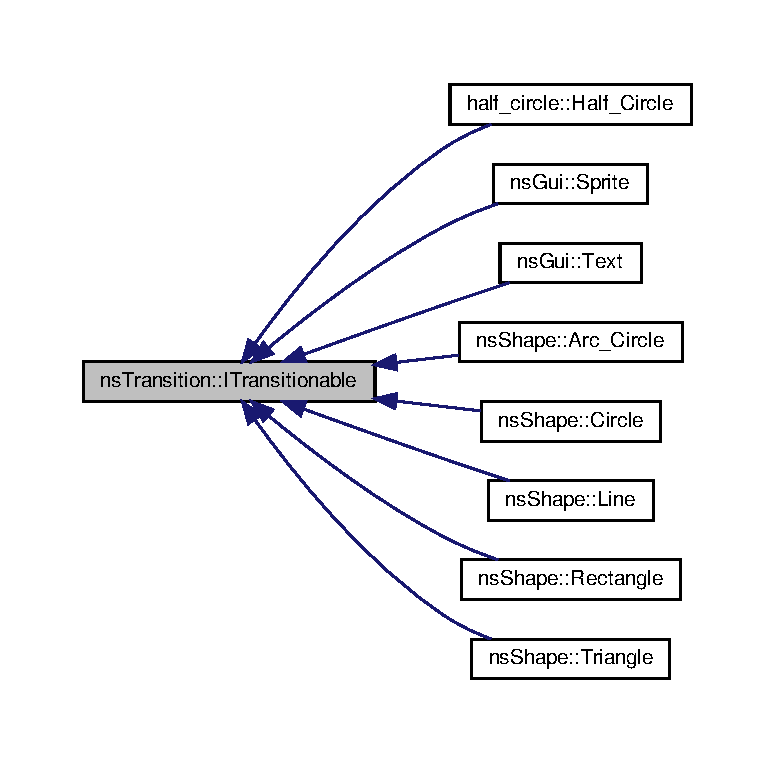
\includegraphics[width=350pt]{classns_transition_1_1_i_transitionable__inherit__graph}
\end{center}
\end{figure}
\subsection*{Public Member Functions}
\begin{DoxyCompactItemize}
\item 
virtual \hyperlink{classns_transition_1_1_i_transitionable_addd11ff845b6387b07672a64c1b8938e}{$\sim$\+I\+Transitionable} ()
\begin{DoxyCompactList}\small\item\em Destructeur pour la classe \hyperlink{classns_transition_1_1_i_transitionable}{I\+Transitionable}. \end{DoxyCompactList}\item 
virtual void \hyperlink{classns_transition_1_1_i_transitionable_a5871a16fd47c1e5c8bacdd5da8597ed9}{get\+Values} (const int \&id, std\+::vector$<$ float $>$ \&values)=0
\begin{DoxyCompactList}\small\item\em Récupère des valeurs dans un vecteur de float pour l\textquotesingle{}ID spécifié \end{DoxyCompactList}\item 
virtual void \hyperlink{classns_transition_1_1_i_transitionable_ade37d29f7f2ca4890ed0e2e64d033197}{set\+Values} (const int \&id, const std\+::vector$<$ float $>$ \&values)=0
\begin{DoxyCompactList}\small\item\em Définit les nouvelles valeurs pour l\textquotesingle{}ID spécifié \end{DoxyCompactList}\end{DoxyCompactItemize}


\subsection{Detailed Description}
Une classe abstraite pour n\textquotesingle{}importe quelle élément pouvant effectuer une transition entre deux états. 

Definition at line 23 of file itransitionable.\+h.



\subsection{Constructor \& Destructor Documentation}
\mbox{\Hypertarget{classns_transition_1_1_i_transitionable_addd11ff845b6387b07672a64c1b8938e}\label{classns_transition_1_1_i_transitionable_addd11ff845b6387b07672a64c1b8938e}} 
\index{ns\+Transition\+::\+I\+Transitionable@{ns\+Transition\+::\+I\+Transitionable}!````~I\+Transitionable@{$\sim$\+I\+Transitionable}}
\index{````~I\+Transitionable@{$\sim$\+I\+Transitionable}!ns\+Transition\+::\+I\+Transitionable@{ns\+Transition\+::\+I\+Transitionable}}
\subsubsection{\texorpdfstring{$\sim$\+I\+Transitionable()}{~ITransitionable()}}
{\footnotesize\ttfamily ns\+Transition\+::\+I\+Transitionable\+::$\sim$\+I\+Transitionable (\begin{DoxyParamCaption}{ }\end{DoxyParamCaption})\hspace{0.3cm}{\ttfamily [inline]}, {\ttfamily [virtual]}}



Destructeur pour la classe \hyperlink{classns_transition_1_1_i_transitionable}{I\+Transitionable}. 



Definition at line 30 of file itransitionable.\+h.



\subsection{Member Function Documentation}
\mbox{\Hypertarget{classns_transition_1_1_i_transitionable_a5871a16fd47c1e5c8bacdd5da8597ed9}\label{classns_transition_1_1_i_transitionable_a5871a16fd47c1e5c8bacdd5da8597ed9}} 
\index{ns\+Transition\+::\+I\+Transitionable@{ns\+Transition\+::\+I\+Transitionable}!get\+Values@{get\+Values}}
\index{get\+Values@{get\+Values}!ns\+Transition\+::\+I\+Transitionable@{ns\+Transition\+::\+I\+Transitionable}}
\subsubsection{\texorpdfstring{get\+Values()}{getValues()}}
{\footnotesize\ttfamily void ns\+Transition\+::\+I\+Transitionable\+::get\+Values (\begin{DoxyParamCaption}\item[{const int \&}]{id,  }\item[{std\+::vector$<$ float $>$ \&}]{values }\end{DoxyParamCaption})\hspace{0.3cm}{\ttfamily [pure virtual]}}



Récupère des valeurs dans un vecteur de float pour l\textquotesingle{}ID spécifié 


\begin{DoxyParams}[1]{Parameters}
\mbox{\tt in}  & {\em id} & ID des valeurs a récupérer \\
\hline
\mbox{\tt in,out}  & {\em values} & Vecteur de valeurs a peupler \\
\hline
\end{DoxyParams}


Implemented in \hyperlink{classns_gui_1_1_text_a4e23cbbe0345c0742c228d3ab98967c5}{ns\+Gui\+::\+Text}, \hyperlink{classns_shape_1_1_rectangle_a379d73a44d0601a12f26d4867e4246d8}{ns\+Shape\+::\+Rectangle}, \hyperlink{classns_shape_1_1_arc___circle_a11a5569112bf39b90192c7d7e0678736}{ns\+Shape\+::\+Arc\+\_\+\+Circle}, \hyperlink{classns_shape_1_1_triangle_a745ce53bf673b56a23a30f732a041834}{ns\+Shape\+::\+Triangle}, \hyperlink{classns_shape_1_1_line_a572149171c74fb9453c3e2f4093ec466}{ns\+Shape\+::\+Line}, \hyperlink{classhalf__circle_1_1_half___circle_a32fbc3cf8c53b5a239c56b0be6df3e7e}{half\+\_\+circle\+::\+Half\+\_\+\+Circle}, \hyperlink{classns_shape_1_1_circle_a2d126b4d87ea0b141cf1bac7150f760e}{ns\+Shape\+::\+Circle}, and \hyperlink{classns_gui_1_1_sprite_a19cd382e454660efd8a20ee30ba3cc8c}{ns\+Gui\+::\+Sprite}.

\mbox{\Hypertarget{classns_transition_1_1_i_transitionable_ade37d29f7f2ca4890ed0e2e64d033197}\label{classns_transition_1_1_i_transitionable_ade37d29f7f2ca4890ed0e2e64d033197}} 
\index{ns\+Transition\+::\+I\+Transitionable@{ns\+Transition\+::\+I\+Transitionable}!set\+Values@{set\+Values}}
\index{set\+Values@{set\+Values}!ns\+Transition\+::\+I\+Transitionable@{ns\+Transition\+::\+I\+Transitionable}}
\subsubsection{\texorpdfstring{set\+Values()}{setValues()}}
{\footnotesize\ttfamily void ns\+Transition\+::\+I\+Transitionable\+::set\+Values (\begin{DoxyParamCaption}\item[{const int \&}]{id,  }\item[{const std\+::vector$<$ float $>$ \&}]{values }\end{DoxyParamCaption})\hspace{0.3cm}{\ttfamily [pure virtual]}}



Définit les nouvelles valeurs pour l\textquotesingle{}ID spécifié 


\begin{DoxyParams}[1]{Parameters}
\mbox{\tt in}  & {\em id} & ID des valeurs a définir \\
\hline
\mbox{\tt in}  & {\em values} & Vecteur des nouvelles valeurs a appliquer \\
\hline
\end{DoxyParams}


Implemented in \hyperlink{classns_gui_1_1_text_ac1145b3ef4722b7cc9ae111372b84576}{ns\+Gui\+::\+Text}, \hyperlink{classns_shape_1_1_rectangle_a9fcdc9a8adbc91cd2613a0d50058f829}{ns\+Shape\+::\+Rectangle}, \hyperlink{classns_shape_1_1_arc___circle_aa59b45d2a10ec5f8fd030d4ec46721b6}{ns\+Shape\+::\+Arc\+\_\+\+Circle}, \hyperlink{classns_shape_1_1_triangle_af1c6cb0d5d12d8df0bd66c46ec793b22}{ns\+Shape\+::\+Triangle}, \hyperlink{classns_shape_1_1_line_a9984a9a1e69256065de1bd0cc51d2e8f}{ns\+Shape\+::\+Line}, \hyperlink{classhalf__circle_1_1_half___circle_ab128d56c2d348524d88da23b89bf3d35}{half\+\_\+circle\+::\+Half\+\_\+\+Circle}, \hyperlink{classns_shape_1_1_circle_a3edfd0468ef78f456c4fc4fd57c84cdf}{ns\+Shape\+::\+Circle}, and \hyperlink{classns_gui_1_1_sprite_a4259e3283228980136e06d2a41a75d31}{ns\+Gui\+::\+Sprite}.



The documentation for this class was generated from the following file\+:\begin{DoxyCompactItemize}
\item 
libs/mingl/transition/\hyperlink{itransitionable_8h}{itransitionable.\+h}\end{DoxyCompactItemize}

\hypertarget{classns_shape_1_1_line}{}\section{ns\+Shape\+:\+:Line Class Reference}
\label{classns_shape_1_1_line}\index{ns\+Shape\+::\+Line@{ns\+Shape\+::\+Line}}


Classe représentant une ligne.  




{\ttfamily \#include $<$line.\+h$>$}



Inheritance diagram for ns\+Shape\+:\+:Line\+:
\nopagebreak
\begin{figure}[H]
\begin{center}
\leavevmode
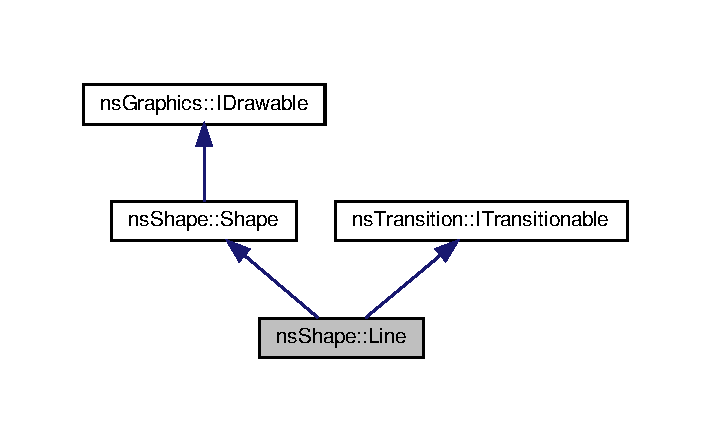
\includegraphics[width=341pt]{classns_shape_1_1_line__inherit__graph}
\end{center}
\end{figure}


Collaboration diagram for ns\+Shape\+:\+:Line\+:
\nopagebreak
\begin{figure}[H]
\begin{center}
\leavevmode
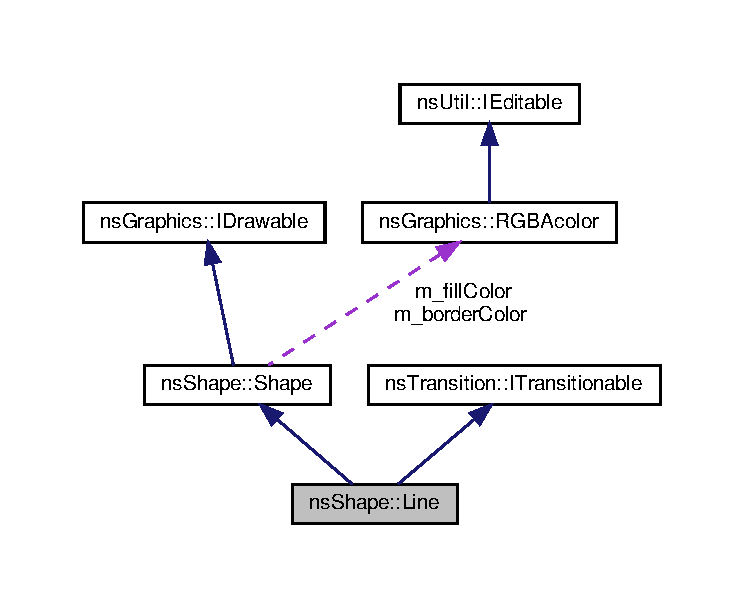
\includegraphics[width=350pt]{classns_shape_1_1_line__coll__graph}
\end{center}
\end{figure}
\subsection*{Public Types}
\begin{DoxyCompactItemize}
\item 
enum \hyperlink{classns_shape_1_1_line_a446a1bbc370b3426afe05f22b681ea58}{Transition\+Ids} \{ \newline
\hyperlink{classns_shape_1_1_line_a446a1bbc370b3426afe05f22b681ea58a9f84f457c9a24574ae17018656830364}{T\+R\+A\+N\+S\+I\+T\+I\+O\+N\+\_\+\+F\+I\+L\+L\+\_\+\+C\+O\+L\+O\+R\+\_\+\+R\+GB}, 
\hyperlink{classns_shape_1_1_line_a446a1bbc370b3426afe05f22b681ea58a2860b432942d04ad21cf17a11776b748}{T\+R\+A\+N\+S\+I\+T\+I\+O\+N\+\_\+\+F\+I\+L\+L\+\_\+\+C\+O\+L\+O\+R\+\_\+\+A\+L\+P\+HA}, 
\hyperlink{classns_shape_1_1_line_a446a1bbc370b3426afe05f22b681ea58ab4facc5aca748b4570273d0b13813dda}{T\+R\+A\+N\+S\+I\+T\+I\+O\+N\+\_\+\+B\+O\+R\+D\+E\+R\+\_\+\+C\+O\+L\+O\+R\+\_\+\+R\+GB}, 
\hyperlink{classns_shape_1_1_line_a446a1bbc370b3426afe05f22b681ea58ad2f2a6854611b0b18a8d1805cfca13f1}{T\+R\+A\+N\+S\+I\+T\+I\+O\+N\+\_\+\+B\+O\+R\+D\+E\+R\+\_\+\+C\+O\+L\+O\+R\+\_\+\+A\+L\+P\+HA}, 
\newline
\hyperlink{classns_shape_1_1_line_a446a1bbc370b3426afe05f22b681ea58ade8f8b210eda14b4f6e940f8f72346f8}{T\+R\+A\+N\+S\+I\+T\+I\+O\+N\+\_\+\+F\+I\+R\+S\+T\+\_\+\+P\+O\+S\+I\+T\+I\+ON}, 
\hyperlink{classns_shape_1_1_line_a446a1bbc370b3426afe05f22b681ea58a55cf135d3e37710549d41ae3faf0f80b}{T\+R\+A\+N\+S\+I\+T\+I\+O\+N\+\_\+\+S\+E\+C\+O\+N\+D\+\_\+\+P\+O\+S\+I\+T\+I\+ON}, 
\hyperlink{classns_shape_1_1_line_a446a1bbc370b3426afe05f22b681ea58a58ffbb046bb10ae9ed84a672d9daea03}{T\+R\+A\+N\+S\+I\+T\+I\+O\+N\+\_\+\+L\+I\+N\+E\+\_\+\+W\+I\+D\+TH}
 \}\begin{DoxyCompactList}\small\item\em Transition\+Ids \+: Liste de toutes les transitions que cet élément peut exécuter. \end{DoxyCompactList}
\end{DoxyCompactItemize}
\subsection*{Public Member Functions}
\begin{DoxyCompactItemize}
\item 
\hyperlink{classns_shape_1_1_line_a7e565c06c16396c7dba0f9d9beedcd17}{Line} (const \hyperlink{classns_graphics_1_1_vec2_d}{ns\+Graphics\+::\+Vec2D} \&first\+Position, const \hyperlink{classns_graphics_1_1_vec2_d}{ns\+Graphics\+::\+Vec2D} \&second\+Position, const \hyperlink{classns_graphics_1_1_r_g_b_acolor}{ns\+Graphics\+::\+R\+G\+B\+Acolor} \&fill\+Color, const float \&line\+Width=1.f)
\begin{DoxyCompactList}\small\item\em Constructeur pour la classe \hyperlink{classns_shape_1_1_line}{Line}. \end{DoxyCompactList}\item 
virtual \hyperlink{classns_shape_1_1_line_a5e867a9bf0795b3a89cffb0c84e21b13}{$\sim$\+Line} () override=default
\begin{DoxyCompactList}\small\item\em Destructeur virtuel pour la classe \hyperlink{classns_shape_1_1_line}{Line}. \end{DoxyCompactList}\item 
virtual void \hyperlink{classns_shape_1_1_line_ae14d0de306fa91ee38bafd1d27682beb}{draw} (\hyperlink{class_min_g_l}{Min\+GL} \&window) const override
\begin{DoxyCompactList}\small\item\em Fonction pour afficher l\textquotesingle{}objet. \end{DoxyCompactList}\item 
virtual void \hyperlink{classns_shape_1_1_line_a572149171c74fb9453c3e2f4093ec466}{get\+Values} (const int \&id, std\+::vector$<$ float $>$ \&values) override
\begin{DoxyCompactList}\small\item\em Récupère des valeurs dans un vecteur de float pour l\textquotesingle{}ID spécifié \end{DoxyCompactList}\item 
virtual void \hyperlink{classns_shape_1_1_line_a9984a9a1e69256065de1bd0cc51d2e8f}{set\+Values} (const int \&id, const std\+::vector$<$ float $>$ \&values) override
\begin{DoxyCompactList}\small\item\em Définit les nouvelles valeurs pour l\textquotesingle{}ID spécifié \end{DoxyCompactList}\item 
\hyperlink{classns_shape_1_1_line}{Line} \hyperlink{classns_shape_1_1_line_adddeb7810639aa3eec2756846d40a430}{operator+} (const \hyperlink{classns_graphics_1_1_vec2_d}{ns\+Graphics\+::\+Vec2D} \&position) const
\begin{DoxyCompactList}\small\item\em Opérateur de décalage. \end{DoxyCompactList}\item 
\hyperlink{classns_shape_1_1_line}{Line} \hyperlink{classns_shape_1_1_line_a9686aab308107dff4799ec75a98d3aef}{operator$\ast$} (const float \&f) const
\begin{DoxyCompactList}\small\item\em Opérateur de réduction. \end{DoxyCompactList}\item 
const \hyperlink{classns_graphics_1_1_vec2_d}{ns\+Graphics\+::\+Vec2D} \& \hyperlink{classns_shape_1_1_line_a5e99d542b7557f79f58623b098672fdc}{get\+First\+Position} () const
\begin{DoxyCompactList}\small\item\em Récupère la position du premier sommet de la ligne. \end{DoxyCompactList}\item 
void \hyperlink{classns_shape_1_1_line_a62178d318a6b856e574149f58f9838f9}{set\+First\+Position} (const \hyperlink{classns_graphics_1_1_vec2_d}{ns\+Graphics\+::\+Vec2D} \&first\+Position)
\begin{DoxyCompactList}\small\item\em Définit la nouvelle position du premier sommet de la ligne. \end{DoxyCompactList}\item 
const \hyperlink{classns_graphics_1_1_vec2_d}{ns\+Graphics\+::\+Vec2D} \& \hyperlink{classns_shape_1_1_line_a3e239062daea5c0f247ccd9f454a45e8}{get\+Second\+Position} () const
\begin{DoxyCompactList}\small\item\em Récupère la position du second sommet de la ligne. \end{DoxyCompactList}\item 
void \hyperlink{classns_shape_1_1_line_ac8235be2b90d57497875a4265fc2bdc5}{set\+Second\+Position} (const \hyperlink{classns_graphics_1_1_vec2_d}{ns\+Graphics\+::\+Vec2D} \&second\+Position)
\begin{DoxyCompactList}\small\item\em Définit la nouvelle position du second sommet de la ligne. \end{DoxyCompactList}\item 
float \hyperlink{classns_shape_1_1_line_aab6e3cacd0062c1d5e2e55e9099a617a}{get\+Line\+Width} () const
\begin{DoxyCompactList}\small\item\em Récupère l\textquotesingle{}épaisseur de la ligne. \end{DoxyCompactList}\item 
void \hyperlink{classns_shape_1_1_line_ab98591827289680e28b4b0904e6d95f2}{set\+Line\+Width} (float line\+Width)
\begin{DoxyCompactList}\small\item\em Définit la nouvelle épaisseur de la ligne. \end{DoxyCompactList}\end{DoxyCompactItemize}
\subsection*{Additional Inherited Members}


\subsection{Detailed Description}
Classe représentant une ligne. 

Definition at line 25 of file line.\+h.



\subsection{Member Enumeration Documentation}
\mbox{\Hypertarget{classns_shape_1_1_line_a446a1bbc370b3426afe05f22b681ea58}\label{classns_shape_1_1_line_a446a1bbc370b3426afe05f22b681ea58}} 
\index{ns\+Shape\+::\+Line@{ns\+Shape\+::\+Line}!Transition\+Ids@{Transition\+Ids}}
\index{Transition\+Ids@{Transition\+Ids}!ns\+Shape\+::\+Line@{ns\+Shape\+::\+Line}}
\subsubsection{\texorpdfstring{Transition\+Ids}{TransitionIds}}
{\footnotesize\ttfamily enum \hyperlink{classns_shape_1_1_line_a446a1bbc370b3426afe05f22b681ea58}{ns\+Shape\+::\+Line\+::\+Transition\+Ids}}



Transition\+Ids \+: Liste de toutes les transitions que cet élément peut exécuter. 

\begin{DoxyEnumFields}{Enumerator}
\raisebox{\heightof{T}}[0pt][0pt]{\index{T\+R\+A\+N\+S\+I\+T\+I\+O\+N\+\_\+\+F\+I\+L\+L\+\_\+\+C\+O\+L\+O\+R\+\_\+\+R\+GB@{T\+R\+A\+N\+S\+I\+T\+I\+O\+N\+\_\+\+F\+I\+L\+L\+\_\+\+C\+O\+L\+O\+R\+\_\+\+R\+GB}!ns\+Shape\+::\+Line@{ns\+Shape\+::\+Line}}\index{ns\+Shape\+::\+Line@{ns\+Shape\+::\+Line}!T\+R\+A\+N\+S\+I\+T\+I\+O\+N\+\_\+\+F\+I\+L\+L\+\_\+\+C\+O\+L\+O\+R\+\_\+\+R\+GB@{T\+R\+A\+N\+S\+I\+T\+I\+O\+N\+\_\+\+F\+I\+L\+L\+\_\+\+C\+O\+L\+O\+R\+\_\+\+R\+GB}}}\mbox{\Hypertarget{classns_shape_1_1_line_a446a1bbc370b3426afe05f22b681ea58a9f84f457c9a24574ae17018656830364}\label{classns_shape_1_1_line_a446a1bbc370b3426afe05f22b681ea58a9f84f457c9a24574ae17018656830364}} 
T\+R\+A\+N\+S\+I\+T\+I\+O\+N\+\_\+\+F\+I\+L\+L\+\_\+\+C\+O\+L\+O\+R\+\_\+\+R\+GB&Transition pour la couleur de remplissage \\
\hline

\raisebox{\heightof{T}}[0pt][0pt]{\index{T\+R\+A\+N\+S\+I\+T\+I\+O\+N\+\_\+\+F\+I\+L\+L\+\_\+\+C\+O\+L\+O\+R\+\_\+\+A\+L\+P\+HA@{T\+R\+A\+N\+S\+I\+T\+I\+O\+N\+\_\+\+F\+I\+L\+L\+\_\+\+C\+O\+L\+O\+R\+\_\+\+A\+L\+P\+HA}!ns\+Shape\+::\+Line@{ns\+Shape\+::\+Line}}\index{ns\+Shape\+::\+Line@{ns\+Shape\+::\+Line}!T\+R\+A\+N\+S\+I\+T\+I\+O\+N\+\_\+\+F\+I\+L\+L\+\_\+\+C\+O\+L\+O\+R\+\_\+\+A\+L\+P\+HA@{T\+R\+A\+N\+S\+I\+T\+I\+O\+N\+\_\+\+F\+I\+L\+L\+\_\+\+C\+O\+L\+O\+R\+\_\+\+A\+L\+P\+HA}}}\mbox{\Hypertarget{classns_shape_1_1_line_a446a1bbc370b3426afe05f22b681ea58a2860b432942d04ad21cf17a11776b748}\label{classns_shape_1_1_line_a446a1bbc370b3426afe05f22b681ea58a2860b432942d04ad21cf17a11776b748}} 
T\+R\+A\+N\+S\+I\+T\+I\+O\+N\+\_\+\+F\+I\+L\+L\+\_\+\+C\+O\+L\+O\+R\+\_\+\+A\+L\+P\+HA&Transition pour la transparence de remplissage \\
\hline

\raisebox{\heightof{T}}[0pt][0pt]{\index{T\+R\+A\+N\+S\+I\+T\+I\+O\+N\+\_\+\+B\+O\+R\+D\+E\+R\+\_\+\+C\+O\+L\+O\+R\+\_\+\+R\+GB@{T\+R\+A\+N\+S\+I\+T\+I\+O\+N\+\_\+\+B\+O\+R\+D\+E\+R\+\_\+\+C\+O\+L\+O\+R\+\_\+\+R\+GB}!ns\+Shape\+::\+Line@{ns\+Shape\+::\+Line}}\index{ns\+Shape\+::\+Line@{ns\+Shape\+::\+Line}!T\+R\+A\+N\+S\+I\+T\+I\+O\+N\+\_\+\+B\+O\+R\+D\+E\+R\+\_\+\+C\+O\+L\+O\+R\+\_\+\+R\+GB@{T\+R\+A\+N\+S\+I\+T\+I\+O\+N\+\_\+\+B\+O\+R\+D\+E\+R\+\_\+\+C\+O\+L\+O\+R\+\_\+\+R\+GB}}}\mbox{\Hypertarget{classns_shape_1_1_line_a446a1bbc370b3426afe05f22b681ea58ab4facc5aca748b4570273d0b13813dda}\label{classns_shape_1_1_line_a446a1bbc370b3426afe05f22b681ea58ab4facc5aca748b4570273d0b13813dda}} 
T\+R\+A\+N\+S\+I\+T\+I\+O\+N\+\_\+\+B\+O\+R\+D\+E\+R\+\_\+\+C\+O\+L\+O\+R\+\_\+\+R\+GB&Transition pour la couleur de bord \\
\hline

\raisebox{\heightof{T}}[0pt][0pt]{\index{T\+R\+A\+N\+S\+I\+T\+I\+O\+N\+\_\+\+B\+O\+R\+D\+E\+R\+\_\+\+C\+O\+L\+O\+R\+\_\+\+A\+L\+P\+HA@{T\+R\+A\+N\+S\+I\+T\+I\+O\+N\+\_\+\+B\+O\+R\+D\+E\+R\+\_\+\+C\+O\+L\+O\+R\+\_\+\+A\+L\+P\+HA}!ns\+Shape\+::\+Line@{ns\+Shape\+::\+Line}}\index{ns\+Shape\+::\+Line@{ns\+Shape\+::\+Line}!T\+R\+A\+N\+S\+I\+T\+I\+O\+N\+\_\+\+B\+O\+R\+D\+E\+R\+\_\+\+C\+O\+L\+O\+R\+\_\+\+A\+L\+P\+HA@{T\+R\+A\+N\+S\+I\+T\+I\+O\+N\+\_\+\+B\+O\+R\+D\+E\+R\+\_\+\+C\+O\+L\+O\+R\+\_\+\+A\+L\+P\+HA}}}\mbox{\Hypertarget{classns_shape_1_1_line_a446a1bbc370b3426afe05f22b681ea58ad2f2a6854611b0b18a8d1805cfca13f1}\label{classns_shape_1_1_line_a446a1bbc370b3426afe05f22b681ea58ad2f2a6854611b0b18a8d1805cfca13f1}} 
T\+R\+A\+N\+S\+I\+T\+I\+O\+N\+\_\+\+B\+O\+R\+D\+E\+R\+\_\+\+C\+O\+L\+O\+R\+\_\+\+A\+L\+P\+HA&Transition pour la transparence de bord \\
\hline

\raisebox{\heightof{T}}[0pt][0pt]{\index{T\+R\+A\+N\+S\+I\+T\+I\+O\+N\+\_\+\+F\+I\+R\+S\+T\+\_\+\+P\+O\+S\+I\+T\+I\+ON@{T\+R\+A\+N\+S\+I\+T\+I\+O\+N\+\_\+\+F\+I\+R\+S\+T\+\_\+\+P\+O\+S\+I\+T\+I\+ON}!ns\+Shape\+::\+Line@{ns\+Shape\+::\+Line}}\index{ns\+Shape\+::\+Line@{ns\+Shape\+::\+Line}!T\+R\+A\+N\+S\+I\+T\+I\+O\+N\+\_\+\+F\+I\+R\+S\+T\+\_\+\+P\+O\+S\+I\+T\+I\+ON@{T\+R\+A\+N\+S\+I\+T\+I\+O\+N\+\_\+\+F\+I\+R\+S\+T\+\_\+\+P\+O\+S\+I\+T\+I\+ON}}}\mbox{\Hypertarget{classns_shape_1_1_line_a446a1bbc370b3426afe05f22b681ea58ade8f8b210eda14b4f6e940f8f72346f8}\label{classns_shape_1_1_line_a446a1bbc370b3426afe05f22b681ea58ade8f8b210eda14b4f6e940f8f72346f8}} 
T\+R\+A\+N\+S\+I\+T\+I\+O\+N\+\_\+\+F\+I\+R\+S\+T\+\_\+\+P\+O\+S\+I\+T\+I\+ON&Transition pour la position du premier sommet \\
\hline

\raisebox{\heightof{T}}[0pt][0pt]{\index{T\+R\+A\+N\+S\+I\+T\+I\+O\+N\+\_\+\+S\+E\+C\+O\+N\+D\+\_\+\+P\+O\+S\+I\+T\+I\+ON@{T\+R\+A\+N\+S\+I\+T\+I\+O\+N\+\_\+\+S\+E\+C\+O\+N\+D\+\_\+\+P\+O\+S\+I\+T\+I\+ON}!ns\+Shape\+::\+Line@{ns\+Shape\+::\+Line}}\index{ns\+Shape\+::\+Line@{ns\+Shape\+::\+Line}!T\+R\+A\+N\+S\+I\+T\+I\+O\+N\+\_\+\+S\+E\+C\+O\+N\+D\+\_\+\+P\+O\+S\+I\+T\+I\+ON@{T\+R\+A\+N\+S\+I\+T\+I\+O\+N\+\_\+\+S\+E\+C\+O\+N\+D\+\_\+\+P\+O\+S\+I\+T\+I\+ON}}}\mbox{\Hypertarget{classns_shape_1_1_line_a446a1bbc370b3426afe05f22b681ea58a55cf135d3e37710549d41ae3faf0f80b}\label{classns_shape_1_1_line_a446a1bbc370b3426afe05f22b681ea58a55cf135d3e37710549d41ae3faf0f80b}} 
T\+R\+A\+N\+S\+I\+T\+I\+O\+N\+\_\+\+S\+E\+C\+O\+N\+D\+\_\+\+P\+O\+S\+I\+T\+I\+ON&Transition pour la position du second sommet \\
\hline

\raisebox{\heightof{T}}[0pt][0pt]{\index{T\+R\+A\+N\+S\+I\+T\+I\+O\+N\+\_\+\+L\+I\+N\+E\+\_\+\+W\+I\+D\+TH@{T\+R\+A\+N\+S\+I\+T\+I\+O\+N\+\_\+\+L\+I\+N\+E\+\_\+\+W\+I\+D\+TH}!ns\+Shape\+::\+Line@{ns\+Shape\+::\+Line}}\index{ns\+Shape\+::\+Line@{ns\+Shape\+::\+Line}!T\+R\+A\+N\+S\+I\+T\+I\+O\+N\+\_\+\+L\+I\+N\+E\+\_\+\+W\+I\+D\+TH@{T\+R\+A\+N\+S\+I\+T\+I\+O\+N\+\_\+\+L\+I\+N\+E\+\_\+\+W\+I\+D\+TH}}}\mbox{\Hypertarget{classns_shape_1_1_line_a446a1bbc370b3426afe05f22b681ea58a58ffbb046bb10ae9ed84a672d9daea03}\label{classns_shape_1_1_line_a446a1bbc370b3426afe05f22b681ea58a58ffbb046bb10ae9ed84a672d9daea03}} 
T\+R\+A\+N\+S\+I\+T\+I\+O\+N\+\_\+\+L\+I\+N\+E\+\_\+\+W\+I\+D\+TH&Transition pour l\textquotesingle{}épaisseur de la ligne \\
\hline

\end{DoxyEnumFields}


Definition at line 32 of file line.\+h.



\subsection{Constructor \& Destructor Documentation}
\mbox{\Hypertarget{classns_shape_1_1_line_a7e565c06c16396c7dba0f9d9beedcd17}\label{classns_shape_1_1_line_a7e565c06c16396c7dba0f9d9beedcd17}} 
\index{ns\+Shape\+::\+Line@{ns\+Shape\+::\+Line}!Line@{Line}}
\index{Line@{Line}!ns\+Shape\+::\+Line@{ns\+Shape\+::\+Line}}
\subsubsection{\texorpdfstring{Line()}{Line()}}
{\footnotesize\ttfamily ns\+Shape\+::\+Line\+::\+Line (\begin{DoxyParamCaption}\item[{const \hyperlink{classns_graphics_1_1_vec2_d}{ns\+Graphics\+::\+Vec2D} \&}]{first\+Position,  }\item[{const \hyperlink{classns_graphics_1_1_vec2_d}{ns\+Graphics\+::\+Vec2D} \&}]{second\+Position,  }\item[{const \hyperlink{classns_graphics_1_1_r_g_b_acolor}{ns\+Graphics\+::\+R\+G\+B\+Acolor} \&}]{fill\+Color,  }\item[{const float \&}]{line\+Width = {\ttfamily 1.f} }\end{DoxyParamCaption})}



Constructeur pour la classe \hyperlink{classns_shape_1_1_line}{Line}. 


\begin{DoxyParams}[1]{Parameters}
\mbox{\tt in}  & {\em first\+Position} & \+: Position du premier sommet \\
\hline
\mbox{\tt in}  & {\em second\+Position} & \+: Position du second sommet \\
\hline
\mbox{\tt in}  & {\em fill\+Color} & \+: Couleur de remplissage \\
\hline
\mbox{\tt in}  & {\em line\+Width} & \+: Epaisseur de la ligne \\
\hline
\end{DoxyParams}
\mbox{\Hypertarget{classns_shape_1_1_line_a5e867a9bf0795b3a89cffb0c84e21b13}\label{classns_shape_1_1_line_a5e867a9bf0795b3a89cffb0c84e21b13}} 
\index{ns\+Shape\+::\+Line@{ns\+Shape\+::\+Line}!````~Line@{$\sim$\+Line}}
\index{````~Line@{$\sim$\+Line}!ns\+Shape\+::\+Line@{ns\+Shape\+::\+Line}}
\subsubsection{\texorpdfstring{$\sim$\+Line()}{~Line()}}
{\footnotesize\ttfamily ns\+Shape\+::\+Line\+::$\sim$\+Line (\begin{DoxyParamCaption}{ }\end{DoxyParamCaption})\hspace{0.3cm}{\ttfamily [override]}, {\ttfamily [virtual]}, {\ttfamily [default]}}



Destructeur virtuel pour la classe \hyperlink{classns_shape_1_1_line}{Line}. 



\subsection{Member Function Documentation}
\mbox{\Hypertarget{classns_shape_1_1_line_ae14d0de306fa91ee38bafd1d27682beb}\label{classns_shape_1_1_line_ae14d0de306fa91ee38bafd1d27682beb}} 
\index{ns\+Shape\+::\+Line@{ns\+Shape\+::\+Line}!draw@{draw}}
\index{draw@{draw}!ns\+Shape\+::\+Line@{ns\+Shape\+::\+Line}}
\subsubsection{\texorpdfstring{draw()}{draw()}}
{\footnotesize\ttfamily virtual void ns\+Shape\+::\+Line\+::draw (\begin{DoxyParamCaption}\item[{\hyperlink{class_min_g_l}{Min\+GL} \&}]{window }\end{DoxyParamCaption}) const\hspace{0.3cm}{\ttfamily [override]}, {\ttfamily [virtual]}}



Fonction pour afficher l\textquotesingle{}objet. 



Implements \hyperlink{classns_graphics_1_1_i_drawable_abed8a61e1d507d31e76f0891f3bf9c51}{ns\+Graphics\+::\+I\+Drawable}.

\mbox{\Hypertarget{classns_shape_1_1_line_a5e99d542b7557f79f58623b098672fdc}\label{classns_shape_1_1_line_a5e99d542b7557f79f58623b098672fdc}} 
\index{ns\+Shape\+::\+Line@{ns\+Shape\+::\+Line}!get\+First\+Position@{get\+First\+Position}}
\index{get\+First\+Position@{get\+First\+Position}!ns\+Shape\+::\+Line@{ns\+Shape\+::\+Line}}
\subsubsection{\texorpdfstring{get\+First\+Position()}{getFirstPosition()}}
{\footnotesize\ttfamily const \hyperlink{classns_graphics_1_1_vec2_d}{ns\+Graphics\+::\+Vec2D} \& ns\+Shape\+::\+Line\+::get\+First\+Position (\begin{DoxyParamCaption}{ }\end{DoxyParamCaption}) const}



Récupère la position du premier sommet de la ligne. 

\mbox{\Hypertarget{classns_shape_1_1_line_aab6e3cacd0062c1d5e2e55e9099a617a}\label{classns_shape_1_1_line_aab6e3cacd0062c1d5e2e55e9099a617a}} 
\index{ns\+Shape\+::\+Line@{ns\+Shape\+::\+Line}!get\+Line\+Width@{get\+Line\+Width}}
\index{get\+Line\+Width@{get\+Line\+Width}!ns\+Shape\+::\+Line@{ns\+Shape\+::\+Line}}
\subsubsection{\texorpdfstring{get\+Line\+Width()}{getLineWidth()}}
{\footnotesize\ttfamily float ns\+Shape\+::\+Line\+::get\+Line\+Width (\begin{DoxyParamCaption}{ }\end{DoxyParamCaption}) const}



Récupère l\textquotesingle{}épaisseur de la ligne. 

\mbox{\Hypertarget{classns_shape_1_1_line_a3e239062daea5c0f247ccd9f454a45e8}\label{classns_shape_1_1_line_a3e239062daea5c0f247ccd9f454a45e8}} 
\index{ns\+Shape\+::\+Line@{ns\+Shape\+::\+Line}!get\+Second\+Position@{get\+Second\+Position}}
\index{get\+Second\+Position@{get\+Second\+Position}!ns\+Shape\+::\+Line@{ns\+Shape\+::\+Line}}
\subsubsection{\texorpdfstring{get\+Second\+Position()}{getSecondPosition()}}
{\footnotesize\ttfamily const \hyperlink{classns_graphics_1_1_vec2_d}{ns\+Graphics\+::\+Vec2D} \& ns\+Shape\+::\+Line\+::get\+Second\+Position (\begin{DoxyParamCaption}{ }\end{DoxyParamCaption}) const}



Récupère la position du second sommet de la ligne. 

\mbox{\Hypertarget{classns_shape_1_1_line_a572149171c74fb9453c3e2f4093ec466}\label{classns_shape_1_1_line_a572149171c74fb9453c3e2f4093ec466}} 
\index{ns\+Shape\+::\+Line@{ns\+Shape\+::\+Line}!get\+Values@{get\+Values}}
\index{get\+Values@{get\+Values}!ns\+Shape\+::\+Line@{ns\+Shape\+::\+Line}}
\subsubsection{\texorpdfstring{get\+Values()}{getValues()}}
{\footnotesize\ttfamily virtual void ns\+Shape\+::\+Line\+::get\+Values (\begin{DoxyParamCaption}\item[{const int \&}]{id,  }\item[{std\+::vector$<$ float $>$ \&}]{values }\end{DoxyParamCaption})\hspace{0.3cm}{\ttfamily [override]}, {\ttfamily [virtual]}}



Récupère des valeurs dans un vecteur de float pour l\textquotesingle{}ID spécifié 


\begin{DoxyParams}[1]{Parameters}
\mbox{\tt in}  & {\em id} & ID des valeurs a récupérer \\
\hline
\mbox{\tt in,out}  & {\em values} & Vecteur de valeurs a peupler \\
\hline
\end{DoxyParams}


Implements \hyperlink{classns_transition_1_1_i_transitionable_a5871a16fd47c1e5c8bacdd5da8597ed9}{ns\+Transition\+::\+I\+Transitionable}.

\mbox{\Hypertarget{classns_shape_1_1_line_a9686aab308107dff4799ec75a98d3aef}\label{classns_shape_1_1_line_a9686aab308107dff4799ec75a98d3aef}} 
\index{ns\+Shape\+::\+Line@{ns\+Shape\+::\+Line}!operator$\ast$@{operator$\ast$}}
\index{operator$\ast$@{operator$\ast$}!ns\+Shape\+::\+Line@{ns\+Shape\+::\+Line}}
\subsubsection{\texorpdfstring{operator$\ast$()}{operator*()}}
{\footnotesize\ttfamily \hyperlink{classns_shape_1_1_line}{Line} ns\+Shape\+::\+Line\+::operator$\ast$ (\begin{DoxyParamCaption}\item[{const float \&}]{f }\end{DoxyParamCaption}) const}



Opérateur de réduction. 


\begin{DoxyParams}[1]{Parameters}
\mbox{\tt in}  & {\em f} & \+: Nombre avec lequel multiplier la position actuelle \\
\hline
\end{DoxyParams}
\mbox{\Hypertarget{classns_shape_1_1_line_adddeb7810639aa3eec2756846d40a430}\label{classns_shape_1_1_line_adddeb7810639aa3eec2756846d40a430}} 
\index{ns\+Shape\+::\+Line@{ns\+Shape\+::\+Line}!operator+@{operator+}}
\index{operator+@{operator+}!ns\+Shape\+::\+Line@{ns\+Shape\+::\+Line}}
\subsubsection{\texorpdfstring{operator+()}{operator+()}}
{\footnotesize\ttfamily \hyperlink{classns_shape_1_1_line}{Line} ns\+Shape\+::\+Line\+::operator+ (\begin{DoxyParamCaption}\item[{const \hyperlink{classns_graphics_1_1_vec2_d}{ns\+Graphics\+::\+Vec2D} \&}]{position }\end{DoxyParamCaption}) const}



Opérateur de décalage. 


\begin{DoxyParams}[1]{Parameters}
\mbox{\tt in}  & {\em position} & \+: Position a additionner \\
\hline
\end{DoxyParams}
\mbox{\Hypertarget{classns_shape_1_1_line_a62178d318a6b856e574149f58f9838f9}\label{classns_shape_1_1_line_a62178d318a6b856e574149f58f9838f9}} 
\index{ns\+Shape\+::\+Line@{ns\+Shape\+::\+Line}!set\+First\+Position@{set\+First\+Position}}
\index{set\+First\+Position@{set\+First\+Position}!ns\+Shape\+::\+Line@{ns\+Shape\+::\+Line}}
\subsubsection{\texorpdfstring{set\+First\+Position()}{setFirstPosition()}}
{\footnotesize\ttfamily void ns\+Shape\+::\+Line\+::set\+First\+Position (\begin{DoxyParamCaption}\item[{const \hyperlink{classns_graphics_1_1_vec2_d}{ns\+Graphics\+::\+Vec2D} \&}]{first\+Position }\end{DoxyParamCaption})}



Définit la nouvelle position du premier sommet de la ligne. 


\begin{DoxyParams}[1]{Parameters}
\mbox{\tt in}  & {\em first\+Position} & \+: Nouvelle position du premier sommet \\
\hline
\end{DoxyParams}
\mbox{\Hypertarget{classns_shape_1_1_line_ab98591827289680e28b4b0904e6d95f2}\label{classns_shape_1_1_line_ab98591827289680e28b4b0904e6d95f2}} 
\index{ns\+Shape\+::\+Line@{ns\+Shape\+::\+Line}!set\+Line\+Width@{set\+Line\+Width}}
\index{set\+Line\+Width@{set\+Line\+Width}!ns\+Shape\+::\+Line@{ns\+Shape\+::\+Line}}
\subsubsection{\texorpdfstring{set\+Line\+Width()}{setLineWidth()}}
{\footnotesize\ttfamily void ns\+Shape\+::\+Line\+::set\+Line\+Width (\begin{DoxyParamCaption}\item[{float}]{line\+Width }\end{DoxyParamCaption})}



Définit la nouvelle épaisseur de la ligne. 


\begin{DoxyParams}[1]{Parameters}
\mbox{\tt in}  & {\em line\+Width} & \+: Nouvelle épaisseur \\
\hline
\end{DoxyParams}
\mbox{\Hypertarget{classns_shape_1_1_line_ac8235be2b90d57497875a4265fc2bdc5}\label{classns_shape_1_1_line_ac8235be2b90d57497875a4265fc2bdc5}} 
\index{ns\+Shape\+::\+Line@{ns\+Shape\+::\+Line}!set\+Second\+Position@{set\+Second\+Position}}
\index{set\+Second\+Position@{set\+Second\+Position}!ns\+Shape\+::\+Line@{ns\+Shape\+::\+Line}}
\subsubsection{\texorpdfstring{set\+Second\+Position()}{setSecondPosition()}}
{\footnotesize\ttfamily void ns\+Shape\+::\+Line\+::set\+Second\+Position (\begin{DoxyParamCaption}\item[{const \hyperlink{classns_graphics_1_1_vec2_d}{ns\+Graphics\+::\+Vec2D} \&}]{second\+Position }\end{DoxyParamCaption})}



Définit la nouvelle position du second sommet de la ligne. 


\begin{DoxyParams}[1]{Parameters}
\mbox{\tt in}  & {\em second\+Position} & \+: Nouvelle position du second sommet \\
\hline
\end{DoxyParams}
\mbox{\Hypertarget{classns_shape_1_1_line_a9984a9a1e69256065de1bd0cc51d2e8f}\label{classns_shape_1_1_line_a9984a9a1e69256065de1bd0cc51d2e8f}} 
\index{ns\+Shape\+::\+Line@{ns\+Shape\+::\+Line}!set\+Values@{set\+Values}}
\index{set\+Values@{set\+Values}!ns\+Shape\+::\+Line@{ns\+Shape\+::\+Line}}
\subsubsection{\texorpdfstring{set\+Values()}{setValues()}}
{\footnotesize\ttfamily virtual void ns\+Shape\+::\+Line\+::set\+Values (\begin{DoxyParamCaption}\item[{const int \&}]{id,  }\item[{const std\+::vector$<$ float $>$ \&}]{values }\end{DoxyParamCaption})\hspace{0.3cm}{\ttfamily [override]}, {\ttfamily [virtual]}}



Définit les nouvelles valeurs pour l\textquotesingle{}ID spécifié 


\begin{DoxyParams}[1]{Parameters}
\mbox{\tt in}  & {\em id} & ID des valeurs a définir \\
\hline
\mbox{\tt in}  & {\em values} & Vecteur des nouvelles valeurs a appliquer \\
\hline
\end{DoxyParams}


Implements \hyperlink{classns_transition_1_1_i_transitionable_ade37d29f7f2ca4890ed0e2e64d033197}{ns\+Transition\+::\+I\+Transitionable}.



The documentation for this class was generated from the following file\+:\begin{DoxyCompactItemize}
\item 
libs/mingl/shape/\hyperlink{line_8h}{line.\+h}\end{DoxyCompactItemize}

\hypertarget{class_min_g_l}{}\section{Min\+GL Class Reference}
\label{class_min_g_l}\index{Min\+GL@{Min\+GL}}


Classe de base de min\+GL 2.  




{\ttfamily \#include $<$mingl.\+h$>$}

\subsection*{Public Types}
\begin{DoxyCompactItemize}
\item 
typedef std\+::pair$<$ unsigned, bool $>$ \hyperlink{class_min_g_l_a6e612d21ed9723c37ad91093f7b48c96}{Key\+Type\+\_\+t}
\begin{DoxyCompactList}\small\item\em Key\+Type\+\_\+t \+: Représente une touche du clavier. \end{DoxyCompactList}\item 
typedef std\+::map$<$ \hyperlink{class_min_g_l_a6e612d21ed9723c37ad91093f7b48c96}{Key\+Type\+\_\+t}, bool $>$ \hyperlink{class_min_g_l_a084b1a739a671ad7d6af07792bd56af1}{Key\+Map\+\_\+t}
\begin{DoxyCompactList}\small\item\em Key\+Map\+\_\+t \+: Map représentant des touches et leurs état (pressée ou non). \end{DoxyCompactList}\end{DoxyCompactItemize}
\subsection*{Public Member Functions}
\begin{DoxyCompactItemize}
\item 
\hyperlink{class_min_g_l_aecc35a286d1adbcbdc76bf26df18169c}{Min\+GL} (const std\+::string \&name, const \hyperlink{classns_graphics_1_1_vec2_d}{ns\+Graphics\+::\+Vec2D} \&window\+Size=\hyperlink{classns_graphics_1_1_vec2_d}{ns\+Graphics\+::\+Vec2D}(640, 480), const \hyperlink{classns_graphics_1_1_vec2_d}{ns\+Graphics\+::\+Vec2D} \&window\+Position=\hyperlink{classns_graphics_1_1_vec2_d}{ns\+Graphics\+::\+Vec2D}(128, 128), const \hyperlink{classns_graphics_1_1_r_g_b_acolor}{ns\+Graphics\+::\+R\+G\+B\+Acolor} \&background\+Color=\hyperlink{namespacens_graphics_a8c5fcb477a548c6ed321748ec8383bb2}{ns\+Graphics\+::\+K\+White})
\begin{DoxyCompactList}\small\item\em Constructeur pour la classe \hyperlink{class_min_g_l}{Min\+GL}. \end{DoxyCompactList}\item 
\hyperlink{class_min_g_l_a0f84e59dd311785a7e6da848abd5d188}{$\sim$\+Min\+GL} ()
\begin{DoxyCompactList}\small\item\em Destructeur de la classe \hyperlink{class_min_g_l}{Min\+GL}. \end{DoxyCompactList}\item 
void \hyperlink{class_min_g_l_a5962a0a0ced7879bc0cc65e267e8d7fc}{init\+Graphic} ()
\begin{DoxyCompactList}\small\item\em Initialise min\+GL et ouvre la fenêtre. \end{DoxyCompactList}\item 
void \hyperlink{class_min_g_l_a9508f3ac9d4cb4f444f56f5d77ed9d86}{stop\+Graphic} ()
\begin{DoxyCompactList}\small\item\em Ferme la fenêtre et min\+GL proprement. \end{DoxyCompactList}\item 
bool \hyperlink{class_min_g_l_a8f0833403a4fb3df8010c132e81b207f}{is\+Pressed} (const \hyperlink{class_min_g_l_a6e612d21ed9723c37ad91093f7b48c96}{Key\+Type\+\_\+t} \&key)
\begin{DoxyCompactList}\small\item\em Renvoie l\textquotesingle{}état d\textquotesingle{}une touche du clavier (pressée ou non) \end{DoxyCompactList}\item 
void \hyperlink{class_min_g_l_a99750fd4c8f97cfe693b1acb903424cf}{reset\+Key} (const \hyperlink{class_min_g_l_a6e612d21ed9723c37ad91093f7b48c96}{Key\+Type\+\_\+t} \&key)
\begin{DoxyCompactList}\small\item\em Force une touche a être relâchée. \end{DoxyCompactList}\item 
void \hyperlink{class_min_g_l_a489922f0bdde2e38698adddaf57f6eda}{finish\+Frame} ()
\begin{DoxyCompactList}\small\item\em Préviens min\+GL que la frame est terminée. \end{DoxyCompactList}\item 
void \hyperlink{class_min_g_l_a86c940758616957683ffb2e239bba774}{clear\+Screen} ()
\begin{DoxyCompactList}\small\item\em Efface l\textquotesingle{}écran avec la couleur de fond spécifiée. \end{DoxyCompactList}\item 
\hyperlink{classns_event_1_1_event_manager}{ns\+Event\+::\+Event\+Manager} \& \hyperlink{class_min_g_l_ab558253439905930836ab4910a7ae253}{get\+Event\+Manager} ()
\begin{DoxyCompactList}\small\item\em Récupère le gestionnaire d\textquotesingle{}évènements min\+GL. \end{DoxyCompactList}\item 
const \hyperlink{classns_graphics_1_1_r_g_b_acolor}{ns\+Graphics\+::\+R\+G\+B\+Acolor} \& \hyperlink{class_min_g_l_a66758e8e6983cc1dd0b10b1ee743a65a}{get\+Background\+Color} () const
\begin{DoxyCompactList}\small\item\em Récupère la couleur de fond de la fenêtre. \end{DoxyCompactList}\item 
void \hyperlink{class_min_g_l_a4399b7615cea89f850cd5c66e428c367}{set\+Background\+Color} (const \hyperlink{classns_graphics_1_1_r_g_b_acolor}{ns\+Graphics\+::\+R\+G\+B\+Acolor} \&background\+Color)
\begin{DoxyCompactList}\small\item\em Règle la couleur de fond de la fenêtre. \end{DoxyCompactList}\item 
\hyperlink{classns_graphics_1_1_vec2_d}{ns\+Graphics\+::\+Vec2D} \hyperlink{class_min_g_l_a92bacd1567089fb4641ed7b416cfe74d}{get\+Window\+Size} () const
\begin{DoxyCompactList}\small\item\em Récupère la taille de la fenêtre. \end{DoxyCompactList}\item 
void \hyperlink{class_min_g_l_a532d320b7b837998533fe6577ab45bc3}{set\+Window\+Size} (const \hyperlink{classns_graphics_1_1_vec2_d}{ns\+Graphics\+::\+Vec2D} \&window\+Size)
\begin{DoxyCompactList}\small\item\em Règle la taille de la fenêtre. \end{DoxyCompactList}\item 
\hyperlink{classns_graphics_1_1_vec2_d}{ns\+Graphics\+::\+Vec2D} \hyperlink{class_min_g_l_a1ea6ea098988db36f5bf18713f9f3347}{get\+Window\+Position} () const
\begin{DoxyCompactList}\small\item\em Récupère la position de la fenêtre. \end{DoxyCompactList}\item 
void \hyperlink{class_min_g_l_a9239873a52e437457af03f002f5df2b6}{set\+Window\+Position} (const \hyperlink{classns_graphics_1_1_vec2_d}{ns\+Graphics\+::\+Vec2D} \&window\+Position)
\begin{DoxyCompactList}\small\item\em Règle la position de la fenêtre. \end{DoxyCompactList}\item 
const std\+::string \& \hyperlink{class_min_g_l_a46cea08ec9ef4a0678f425000ca77e5b}{get\+Window\+Name} () const
\begin{DoxyCompactList}\small\item\em Récupère le nom de la fenêtre. \end{DoxyCompactList}\item 
void \hyperlink{class_min_g_l_a462ab2edc0eb28990638541873869e0e}{set\+Window\+Name} (const std\+::string \&window\+Name)
\begin{DoxyCompactList}\small\item\em Règle le nom de la fenêtre. \end{DoxyCompactList}\item 
bool \hyperlink{class_min_g_l_a05a0da9d0729e9c7dbd1121b0956866d}{is\+Open} () const
\begin{DoxyCompactList}\small\item\em Retourne si la fenêtre est ouverte. \end{DoxyCompactList}\end{DoxyCompactItemize}
\subsection*{Static Public Member Functions}
\begin{DoxyCompactItemize}
\item 
static void \hyperlink{class_min_g_l_a17c7718b9e966c8147cd56483dcf4e8d}{init\+Glut} ()
\begin{DoxyCompactList}\small\item\em Initialise la bibliothèque freeglut. \end{DoxyCompactList}\end{DoxyCompactItemize}


\subsection{Detailed Description}
Classe de base de min\+GL 2. 

Definition at line 34 of file mingl.\+h.



\subsection{Member Typedef Documentation}
\mbox{\Hypertarget{class_min_g_l_a084b1a739a671ad7d6af07792bd56af1}\label{class_min_g_l_a084b1a739a671ad7d6af07792bd56af1}} 
\index{Min\+GL@{Min\+GL}!Key\+Map\+\_\+t@{Key\+Map\+\_\+t}}
\index{Key\+Map\+\_\+t@{Key\+Map\+\_\+t}!Min\+GL@{Min\+GL}}
\subsubsection{\texorpdfstring{Key\+Map\+\_\+t}{KeyMap\_t}}
{\footnotesize\ttfamily typedef std\+::map$<$\hyperlink{class_min_g_l_a6e612d21ed9723c37ad91093f7b48c96}{Key\+Type\+\_\+t}, bool$>$ \hyperlink{class_min_g_l_a084b1a739a671ad7d6af07792bd56af1}{Min\+G\+L\+::\+Key\+Map\+\_\+t}}



Key\+Map\+\_\+t \+: Map représentant des touches et leurs état (pressée ou non). 

La clé de cette map est un \hyperlink{class_min_g_l_a6e612d21ed9723c37ad91093f7b48c96}{Key\+Type\+\_\+t} représentant une touche, et la valeur est son état. 

Definition at line 55 of file mingl.\+h.

\mbox{\Hypertarget{class_min_g_l_a6e612d21ed9723c37ad91093f7b48c96}\label{class_min_g_l_a6e612d21ed9723c37ad91093f7b48c96}} 
\index{Min\+GL@{Min\+GL}!Key\+Type\+\_\+t@{Key\+Type\+\_\+t}}
\index{Key\+Type\+\_\+t@{Key\+Type\+\_\+t}!Min\+GL@{Min\+GL}}
\subsubsection{\texorpdfstring{Key\+Type\+\_\+t}{KeyType\_t}}
{\footnotesize\ttfamily typedef std\+::pair$<$unsigned, bool$>$ \hyperlink{class_min_g_l_a6e612d21ed9723c37ad91093f7b48c96}{Min\+G\+L\+::\+Key\+Type\+\_\+t}}



Key\+Type\+\_\+t \+: Représente une touche du clavier. 

C\textquotesingle{}est une paire de nombre entier naturel et booléen ~\newline
 
\begin{DoxyItemize}
\item L\textquotesingle{}entier naturel représente le caractère pour une touche non spéciale, ou l\textquotesingle{}identifiant de touche pour une touche spéciale (\href{https://www.opengl.org/resources/libraries/glut/spec3/node54.html}{\tt Voir ici} pour les identifiants).  
\item Le booléen indique si la touche est spéciale ou non.
\end{DoxyItemize}

Definition at line 47 of file mingl.\+h.



\subsection{Constructor \& Destructor Documentation}
\mbox{\Hypertarget{class_min_g_l_aecc35a286d1adbcbdc76bf26df18169c}\label{class_min_g_l_aecc35a286d1adbcbdc76bf26df18169c}} 
\index{Min\+GL@{Min\+GL}!Min\+GL@{Min\+GL}}
\index{Min\+GL@{Min\+GL}!Min\+GL@{Min\+GL}}
\subsubsection{\texorpdfstring{Min\+G\+L()}{MinGL()}}
{\footnotesize\ttfamily Min\+G\+L\+::\+Min\+GL (\begin{DoxyParamCaption}\item[{const std\+::string \&}]{name,  }\item[{const \hyperlink{classns_graphics_1_1_vec2_d}{ns\+Graphics\+::\+Vec2D} \&}]{window\+Size = {\ttfamily \hyperlink{classns_graphics_1_1_vec2_d}{ns\+Graphics\+::\+Vec2D}(640,~480)},  }\item[{const \hyperlink{classns_graphics_1_1_vec2_d}{ns\+Graphics\+::\+Vec2D} \&}]{window\+Position = {\ttfamily \hyperlink{classns_graphics_1_1_vec2_d}{ns\+Graphics\+::\+Vec2D}(128,~128)},  }\item[{const \hyperlink{classns_graphics_1_1_r_g_b_acolor}{ns\+Graphics\+::\+R\+G\+B\+Acolor} \&}]{background\+Color = {\ttfamily \hyperlink{namespacens_graphics_a8c5fcb477a548c6ed321748ec8383bb2}{ns\+Graphics\+::\+K\+White}} }\end{DoxyParamCaption})}



Constructeur pour la classe \hyperlink{class_min_g_l}{Min\+GL}. 


\begin{DoxyParams}[1]{Parameters}
\mbox{\tt in}  & {\em name} & \+: Nom de la fenêtre \\
\hline
\mbox{\tt in}  & {\em window\+Size} & \+: Taille de la fenêtre \\
\hline
\mbox{\tt in}  & {\em window\+Position} & \+: Position de la fenêtre \\
\hline
\mbox{\tt in}  & {\em background\+Color} & \+: Couleur de fond de la fenêtre \\
\hline
\end{DoxyParams}
\mbox{\Hypertarget{class_min_g_l_a0f84e59dd311785a7e6da848abd5d188}\label{class_min_g_l_a0f84e59dd311785a7e6da848abd5d188}} 
\index{Min\+GL@{Min\+GL}!````~Min\+GL@{$\sim$\+Min\+GL}}
\index{````~Min\+GL@{$\sim$\+Min\+GL}!Min\+GL@{Min\+GL}}
\subsubsection{\texorpdfstring{$\sim$\+Min\+G\+L()}{~MinGL()}}
{\footnotesize\ttfamily Min\+G\+L\+::$\sim$\+Min\+GL (\begin{DoxyParamCaption}{ }\end{DoxyParamCaption})}



Destructeur de la classe \hyperlink{class_min_g_l}{Min\+GL}. 



\subsection{Member Function Documentation}
\mbox{\Hypertarget{class_min_g_l_a86c940758616957683ffb2e239bba774}\label{class_min_g_l_a86c940758616957683ffb2e239bba774}} 
\index{Min\+GL@{Min\+GL}!clear\+Screen@{clear\+Screen}}
\index{clear\+Screen@{clear\+Screen}!Min\+GL@{Min\+GL}}
\subsubsection{\texorpdfstring{clear\+Screen()}{clearScreen()}}
{\footnotesize\ttfamily void Min\+G\+L\+::clear\+Screen (\begin{DoxyParamCaption}{ }\end{DoxyParamCaption})}



Efface l\textquotesingle{}écran avec la couleur de fond spécifiée. 

\mbox{\Hypertarget{class_min_g_l_a489922f0bdde2e38698adddaf57f6eda}\label{class_min_g_l_a489922f0bdde2e38698adddaf57f6eda}} 
\index{Min\+GL@{Min\+GL}!finish\+Frame@{finish\+Frame}}
\index{finish\+Frame@{finish\+Frame}!Min\+GL@{Min\+GL}}
\subsubsection{\texorpdfstring{finish\+Frame()}{finishFrame()}}
{\footnotesize\ttfamily void Min\+G\+L\+::finish\+Frame (\begin{DoxyParamCaption}{ }\end{DoxyParamCaption})}



Préviens min\+GL que la frame est terminée. 

\mbox{\Hypertarget{class_min_g_l_a66758e8e6983cc1dd0b10b1ee743a65a}\label{class_min_g_l_a66758e8e6983cc1dd0b10b1ee743a65a}} 
\index{Min\+GL@{Min\+GL}!get\+Background\+Color@{get\+Background\+Color}}
\index{get\+Background\+Color@{get\+Background\+Color}!Min\+GL@{Min\+GL}}
\subsubsection{\texorpdfstring{get\+Background\+Color()}{getBackgroundColor()}}
{\footnotesize\ttfamily const \hyperlink{classns_graphics_1_1_r_g_b_acolor}{ns\+Graphics\+::\+R\+G\+B\+Acolor} \& Min\+G\+L\+::get\+Background\+Color (\begin{DoxyParamCaption}{ }\end{DoxyParamCaption}) const}



Récupère la couleur de fond de la fenêtre. 

\mbox{\Hypertarget{class_min_g_l_ab558253439905930836ab4910a7ae253}\label{class_min_g_l_ab558253439905930836ab4910a7ae253}} 
\index{Min\+GL@{Min\+GL}!get\+Event\+Manager@{get\+Event\+Manager}}
\index{get\+Event\+Manager@{get\+Event\+Manager}!Min\+GL@{Min\+GL}}
\subsubsection{\texorpdfstring{get\+Event\+Manager()}{getEventManager()}}
{\footnotesize\ttfamily \hyperlink{classns_event_1_1_event_manager}{ns\+Event\+::\+Event\+Manager} \& Min\+G\+L\+::get\+Event\+Manager (\begin{DoxyParamCaption}{ }\end{DoxyParamCaption})}



Récupère le gestionnaire d\textquotesingle{}évènements min\+GL. 

\mbox{\Hypertarget{class_min_g_l_a46cea08ec9ef4a0678f425000ca77e5b}\label{class_min_g_l_a46cea08ec9ef4a0678f425000ca77e5b}} 
\index{Min\+GL@{Min\+GL}!get\+Window\+Name@{get\+Window\+Name}}
\index{get\+Window\+Name@{get\+Window\+Name}!Min\+GL@{Min\+GL}}
\subsubsection{\texorpdfstring{get\+Window\+Name()}{getWindowName()}}
{\footnotesize\ttfamily const std\+::string \& Min\+G\+L\+::get\+Window\+Name (\begin{DoxyParamCaption}{ }\end{DoxyParamCaption}) const}



Récupère le nom de la fenêtre. 

\mbox{\Hypertarget{class_min_g_l_a1ea6ea098988db36f5bf18713f9f3347}\label{class_min_g_l_a1ea6ea098988db36f5bf18713f9f3347}} 
\index{Min\+GL@{Min\+GL}!get\+Window\+Position@{get\+Window\+Position}}
\index{get\+Window\+Position@{get\+Window\+Position}!Min\+GL@{Min\+GL}}
\subsubsection{\texorpdfstring{get\+Window\+Position()}{getWindowPosition()}}
{\footnotesize\ttfamily \hyperlink{classns_graphics_1_1_vec2_d}{ns\+Graphics\+::\+Vec2D} Min\+G\+L\+::get\+Window\+Position (\begin{DoxyParamCaption}{ }\end{DoxyParamCaption}) const}



Récupère la position de la fenêtre. 

\mbox{\Hypertarget{class_min_g_l_a92bacd1567089fb4641ed7b416cfe74d}\label{class_min_g_l_a92bacd1567089fb4641ed7b416cfe74d}} 
\index{Min\+GL@{Min\+GL}!get\+Window\+Size@{get\+Window\+Size}}
\index{get\+Window\+Size@{get\+Window\+Size}!Min\+GL@{Min\+GL}}
\subsubsection{\texorpdfstring{get\+Window\+Size()}{getWindowSize()}}
{\footnotesize\ttfamily \hyperlink{classns_graphics_1_1_vec2_d}{ns\+Graphics\+::\+Vec2D} Min\+G\+L\+::get\+Window\+Size (\begin{DoxyParamCaption}{ }\end{DoxyParamCaption}) const}



Récupère la taille de la fenêtre. 

\mbox{\Hypertarget{class_min_g_l_a17c7718b9e966c8147cd56483dcf4e8d}\label{class_min_g_l_a17c7718b9e966c8147cd56483dcf4e8d}} 
\index{Min\+GL@{Min\+GL}!init\+Glut@{init\+Glut}}
\index{init\+Glut@{init\+Glut}!Min\+GL@{Min\+GL}}
\subsubsection{\texorpdfstring{init\+Glut()}{initGlut()}}
{\footnotesize\ttfamily static void Min\+G\+L\+::init\+Glut (\begin{DoxyParamCaption}{ }\end{DoxyParamCaption})\hspace{0.3cm}{\ttfamily [inline]}, {\ttfamily [static]}}



Initialise la bibliothèque freeglut. 



Definition at line 81 of file mingl.\+h.

\mbox{\Hypertarget{class_min_g_l_a5962a0a0ced7879bc0cc65e267e8d7fc}\label{class_min_g_l_a5962a0a0ced7879bc0cc65e267e8d7fc}} 
\index{Min\+GL@{Min\+GL}!init\+Graphic@{init\+Graphic}}
\index{init\+Graphic@{init\+Graphic}!Min\+GL@{Min\+GL}}
\subsubsection{\texorpdfstring{init\+Graphic()}{initGraphic()}}
{\footnotesize\ttfamily void Min\+G\+L\+::init\+Graphic (\begin{DoxyParamCaption}{ }\end{DoxyParamCaption})}



Initialise min\+GL et ouvre la fenêtre. 

\mbox{\Hypertarget{class_min_g_l_a05a0da9d0729e9c7dbd1121b0956866d}\label{class_min_g_l_a05a0da9d0729e9c7dbd1121b0956866d}} 
\index{Min\+GL@{Min\+GL}!is\+Open@{is\+Open}}
\index{is\+Open@{is\+Open}!Min\+GL@{Min\+GL}}
\subsubsection{\texorpdfstring{is\+Open()}{isOpen()}}
{\footnotesize\ttfamily bool Min\+G\+L\+::is\+Open (\begin{DoxyParamCaption}{ }\end{DoxyParamCaption}) const}



Retourne si la fenêtre est ouverte. 

\mbox{\Hypertarget{class_min_g_l_a8f0833403a4fb3df8010c132e81b207f}\label{class_min_g_l_a8f0833403a4fb3df8010c132e81b207f}} 
\index{Min\+GL@{Min\+GL}!is\+Pressed@{is\+Pressed}}
\index{is\+Pressed@{is\+Pressed}!Min\+GL@{Min\+GL}}
\subsubsection{\texorpdfstring{is\+Pressed()}{isPressed()}}
{\footnotesize\ttfamily bool Min\+G\+L\+::is\+Pressed (\begin{DoxyParamCaption}\item[{const \hyperlink{class_min_g_l_a6e612d21ed9723c37ad91093f7b48c96}{Key\+Type\+\_\+t} \&}]{key }\end{DoxyParamCaption})}



Renvoie l\textquotesingle{}état d\textquotesingle{}une touche du clavier (pressée ou non) 


\begin{DoxyParams}[1]{Parameters}
\mbox{\tt in}  & {\em key} & \+: Touche du clavier a vérifier \\
\hline
\end{DoxyParams}
\mbox{\Hypertarget{class_min_g_l_a99750fd4c8f97cfe693b1acb903424cf}\label{class_min_g_l_a99750fd4c8f97cfe693b1acb903424cf}} 
\index{Min\+GL@{Min\+GL}!reset\+Key@{reset\+Key}}
\index{reset\+Key@{reset\+Key}!Min\+GL@{Min\+GL}}
\subsubsection{\texorpdfstring{reset\+Key()}{resetKey()}}
{\footnotesize\ttfamily void Min\+G\+L\+::reset\+Key (\begin{DoxyParamCaption}\item[{const \hyperlink{class_min_g_l_a6e612d21ed9723c37ad91093f7b48c96}{Key\+Type\+\_\+t} \&}]{key }\end{DoxyParamCaption})}



Force une touche a être relâchée. 


\begin{DoxyParams}[1]{Parameters}
\mbox{\tt in}  & {\em key} & \+: Touche du clavier a relâcher \\
\hline
\end{DoxyParams}
\mbox{\Hypertarget{class_min_g_l_a4399b7615cea89f850cd5c66e428c367}\label{class_min_g_l_a4399b7615cea89f850cd5c66e428c367}} 
\index{Min\+GL@{Min\+GL}!set\+Background\+Color@{set\+Background\+Color}}
\index{set\+Background\+Color@{set\+Background\+Color}!Min\+GL@{Min\+GL}}
\subsubsection{\texorpdfstring{set\+Background\+Color()}{setBackgroundColor()}}
{\footnotesize\ttfamily void Min\+G\+L\+::set\+Background\+Color (\begin{DoxyParamCaption}\item[{const \hyperlink{classns_graphics_1_1_r_g_b_acolor}{ns\+Graphics\+::\+R\+G\+B\+Acolor} \&}]{background\+Color }\end{DoxyParamCaption})}



Règle la couleur de fond de la fenêtre. 

\mbox{\Hypertarget{class_min_g_l_a462ab2edc0eb28990638541873869e0e}\label{class_min_g_l_a462ab2edc0eb28990638541873869e0e}} 
\index{Min\+GL@{Min\+GL}!set\+Window\+Name@{set\+Window\+Name}}
\index{set\+Window\+Name@{set\+Window\+Name}!Min\+GL@{Min\+GL}}
\subsubsection{\texorpdfstring{set\+Window\+Name()}{setWindowName()}}
{\footnotesize\ttfamily void Min\+G\+L\+::set\+Window\+Name (\begin{DoxyParamCaption}\item[{const std\+::string \&}]{window\+Name }\end{DoxyParamCaption})}



Règle le nom de la fenêtre. 


\begin{DoxyParams}[1]{Parameters}
\mbox{\tt in}  & {\em window\+Name} & \+: Nouveau nom \\
\hline
\end{DoxyParams}
\mbox{\Hypertarget{class_min_g_l_a9239873a52e437457af03f002f5df2b6}\label{class_min_g_l_a9239873a52e437457af03f002f5df2b6}} 
\index{Min\+GL@{Min\+GL}!set\+Window\+Position@{set\+Window\+Position}}
\index{set\+Window\+Position@{set\+Window\+Position}!Min\+GL@{Min\+GL}}
\subsubsection{\texorpdfstring{set\+Window\+Position()}{setWindowPosition()}}
{\footnotesize\ttfamily void Min\+G\+L\+::set\+Window\+Position (\begin{DoxyParamCaption}\item[{const \hyperlink{classns_graphics_1_1_vec2_d}{ns\+Graphics\+::\+Vec2D} \&}]{window\+Position }\end{DoxyParamCaption})}



Règle la position de la fenêtre. 


\begin{DoxyParams}[1]{Parameters}
\mbox{\tt in}  & {\em window\+Position} & \+: Nouvelle position \\
\hline
\end{DoxyParams}
\mbox{\Hypertarget{class_min_g_l_a532d320b7b837998533fe6577ab45bc3}\label{class_min_g_l_a532d320b7b837998533fe6577ab45bc3}} 
\index{Min\+GL@{Min\+GL}!set\+Window\+Size@{set\+Window\+Size}}
\index{set\+Window\+Size@{set\+Window\+Size}!Min\+GL@{Min\+GL}}
\subsubsection{\texorpdfstring{set\+Window\+Size()}{setWindowSize()}}
{\footnotesize\ttfamily void Min\+G\+L\+::set\+Window\+Size (\begin{DoxyParamCaption}\item[{const \hyperlink{classns_graphics_1_1_vec2_d}{ns\+Graphics\+::\+Vec2D} \&}]{window\+Size }\end{DoxyParamCaption})}



Règle la taille de la fenêtre. 


\begin{DoxyParams}[1]{Parameters}
\mbox{\tt in}  & {\em window\+Size} & \+: Nouvelle taille \\
\hline
\end{DoxyParams}
\mbox{\Hypertarget{class_min_g_l_a9508f3ac9d4cb4f444f56f5d77ed9d86}\label{class_min_g_l_a9508f3ac9d4cb4f444f56f5d77ed9d86}} 
\index{Min\+GL@{Min\+GL}!stop\+Graphic@{stop\+Graphic}}
\index{stop\+Graphic@{stop\+Graphic}!Min\+GL@{Min\+GL}}
\subsubsection{\texorpdfstring{stop\+Graphic()}{stopGraphic()}}
{\footnotesize\ttfamily void Min\+G\+L\+::stop\+Graphic (\begin{DoxyParamCaption}{ }\end{DoxyParamCaption})}



Ferme la fenêtre et min\+GL proprement. 



The documentation for this class was generated from the following file\+:\begin{DoxyCompactItemize}
\item 
libs/mingl/\hyperlink{mingl_8h}{mingl.\+h}\end{DoxyCompactItemize}

\hypertarget{structns_event_1_1_mouse_click_data__t}{}\section{ns\+Event\+:\+:Mouse\+Click\+Data\+\_\+t Struct Reference}
\label{structns_event_1_1_mouse_click_data__t}\index{ns\+Event\+::\+Mouse\+Click\+Data\+\_\+t@{ns\+Event\+::\+Mouse\+Click\+Data\+\_\+t}}


Possède des données pour un événement Mouse\+Click.  




{\ttfamily \#include $<$event.\+hpp$>$}

\subsection*{Public Attributes}
\begin{DoxyCompactItemize}
\item 
int \hyperlink{structns_event_1_1_mouse_click_data__t_a8c4c8e7b68c38ee4819957050bfd2926}{button}
\item 
int \hyperlink{structns_event_1_1_mouse_click_data__t_a81252b916361dc4deab0f42510fdc928}{state}
\item 
int \hyperlink{structns_event_1_1_mouse_click_data__t_a57f8fe6b3c3fb74e0d657158fb24010e}{x}
\item 
int \hyperlink{structns_event_1_1_mouse_click_data__t_a0a2e34034a5b6c8c44087966243fc261}{y}
\end{DoxyCompactItemize}


\subsection{Detailed Description}
Possède des données pour un événement Mouse\+Click. 

Definition at line 33 of file event.\+hpp.



\subsection{Member Data Documentation}
\mbox{\Hypertarget{structns_event_1_1_mouse_click_data__t_a8c4c8e7b68c38ee4819957050bfd2926}\label{structns_event_1_1_mouse_click_data__t_a8c4c8e7b68c38ee4819957050bfd2926}} 
\index{ns\+Event\+::\+Mouse\+Click\+Data\+\_\+t@{ns\+Event\+::\+Mouse\+Click\+Data\+\_\+t}!button@{button}}
\index{button@{button}!ns\+Event\+::\+Mouse\+Click\+Data\+\_\+t@{ns\+Event\+::\+Mouse\+Click\+Data\+\_\+t}}
\subsubsection{\texorpdfstring{button}{button}}
{\footnotesize\ttfamily int ns\+Event\+::\+Mouse\+Click\+Data\+\_\+t\+::button}

ID numérique du bouton 

Definition at line 34 of file event.\+hpp.

\mbox{\Hypertarget{structns_event_1_1_mouse_click_data__t_a81252b916361dc4deab0f42510fdc928}\label{structns_event_1_1_mouse_click_data__t_a81252b916361dc4deab0f42510fdc928}} 
\index{ns\+Event\+::\+Mouse\+Click\+Data\+\_\+t@{ns\+Event\+::\+Mouse\+Click\+Data\+\_\+t}!state@{state}}
\index{state@{state}!ns\+Event\+::\+Mouse\+Click\+Data\+\_\+t@{ns\+Event\+::\+Mouse\+Click\+Data\+\_\+t}}
\subsubsection{\texorpdfstring{state}{state}}
{\footnotesize\ttfamily int ns\+Event\+::\+Mouse\+Click\+Data\+\_\+t\+::state}

Nouvel état du bouton 

Definition at line 35 of file event.\+hpp.

\mbox{\Hypertarget{structns_event_1_1_mouse_click_data__t_a57f8fe6b3c3fb74e0d657158fb24010e}\label{structns_event_1_1_mouse_click_data__t_a57f8fe6b3c3fb74e0d657158fb24010e}} 
\index{ns\+Event\+::\+Mouse\+Click\+Data\+\_\+t@{ns\+Event\+::\+Mouse\+Click\+Data\+\_\+t}!x@{x}}
\index{x@{x}!ns\+Event\+::\+Mouse\+Click\+Data\+\_\+t@{ns\+Event\+::\+Mouse\+Click\+Data\+\_\+t}}
\subsubsection{\texorpdfstring{x}{x}}
{\footnotesize\ttfamily int ns\+Event\+::\+Mouse\+Click\+Data\+\_\+t\+::x}

Coordonnée X du curseur, relative au coin supérieur-\/gauche de la fenêtre 

Definition at line 36 of file event.\+hpp.

\mbox{\Hypertarget{structns_event_1_1_mouse_click_data__t_a0a2e34034a5b6c8c44087966243fc261}\label{structns_event_1_1_mouse_click_data__t_a0a2e34034a5b6c8c44087966243fc261}} 
\index{ns\+Event\+::\+Mouse\+Click\+Data\+\_\+t@{ns\+Event\+::\+Mouse\+Click\+Data\+\_\+t}!y@{y}}
\index{y@{y}!ns\+Event\+::\+Mouse\+Click\+Data\+\_\+t@{ns\+Event\+::\+Mouse\+Click\+Data\+\_\+t}}
\subsubsection{\texorpdfstring{y}{y}}
{\footnotesize\ttfamily int ns\+Event\+::\+Mouse\+Click\+Data\+\_\+t\+::y}

Coordonnée Y du curseur, relative au coin supérieur-\/gauche de la fenêtre 

Definition at line 37 of file event.\+hpp.



The documentation for this struct was generated from the following file\+:\begin{DoxyCompactItemize}
\item 
libs/mingl/event/\hyperlink{event_8hpp}{event.\+hpp}\end{DoxyCompactItemize}

\hypertarget{structns_event_1_1_mouse_move_data__t}{}\section{ns\+Event\+:\+:Mouse\+Move\+Data\+\_\+t Struct Reference}
\label{structns_event_1_1_mouse_move_data__t}\index{ns\+Event\+::\+Mouse\+Move\+Data\+\_\+t@{ns\+Event\+::\+Mouse\+Move\+Data\+\_\+t}}


Possède des données pour un événement Mouse\+Move/\+Mouse\+Drag.  




{\ttfamily \#include $<$event.\+hpp$>$}

\subsection*{Public Attributes}
\begin{DoxyCompactItemize}
\item 
int \hyperlink{structns_event_1_1_mouse_move_data__t_a5093f057977a7d290ead30266c6599fb}{x}
\item 
int \hyperlink{structns_event_1_1_mouse_move_data__t_a9e72b2e9f3c2f68cc33391d076f2c446}{y}
\end{DoxyCompactItemize}


\subsection{Detailed Description}
Possède des données pour un événement Mouse\+Move/\+Mouse\+Drag. 

Definition at line 44 of file event.\+hpp.



\subsection{Member Data Documentation}
\mbox{\Hypertarget{structns_event_1_1_mouse_move_data__t_a5093f057977a7d290ead30266c6599fb}\label{structns_event_1_1_mouse_move_data__t_a5093f057977a7d290ead30266c6599fb}} 
\index{ns\+Event\+::\+Mouse\+Move\+Data\+\_\+t@{ns\+Event\+::\+Mouse\+Move\+Data\+\_\+t}!x@{x}}
\index{x@{x}!ns\+Event\+::\+Mouse\+Move\+Data\+\_\+t@{ns\+Event\+::\+Mouse\+Move\+Data\+\_\+t}}
\subsubsection{\texorpdfstring{x}{x}}
{\footnotesize\ttfamily int ns\+Event\+::\+Mouse\+Move\+Data\+\_\+t\+::x}

Coordonnée X du curseur, relative au coin supérieur-\/gauche de la fenêtre 

Definition at line 45 of file event.\+hpp.

\mbox{\Hypertarget{structns_event_1_1_mouse_move_data__t_a9e72b2e9f3c2f68cc33391d076f2c446}\label{structns_event_1_1_mouse_move_data__t_a9e72b2e9f3c2f68cc33391d076f2c446}} 
\index{ns\+Event\+::\+Mouse\+Move\+Data\+\_\+t@{ns\+Event\+::\+Mouse\+Move\+Data\+\_\+t}!y@{y}}
\index{y@{y}!ns\+Event\+::\+Mouse\+Move\+Data\+\_\+t@{ns\+Event\+::\+Mouse\+Move\+Data\+\_\+t}}
\subsubsection{\texorpdfstring{y}{y}}
{\footnotesize\ttfamily int ns\+Event\+::\+Mouse\+Move\+Data\+\_\+t\+::y}

Coordonnée Y du curseur, relative au coin supérieur-\/gauche de la fenêtre 

Definition at line 46 of file event.\+hpp.



The documentation for this struct was generated from the following file\+:\begin{DoxyCompactItemize}
\item 
libs/mingl/event/\hyperlink{event_8hpp}{event.\+hpp}\end{DoxyCompactItemize}

\hypertarget{structplayer_1_1_player}{}\section{player\+:\+:Player Struct Reference}
\label{structplayer_1_1_player}\index{player\+::\+Player@{player\+::\+Player}}


Structure de joueur pour pouvoir les traiter en instance.  




{\ttfamily \#include $<$player.\+h$>$}



Collaboration diagram for player\+:\+:Player\+:
\nopagebreak
\begin{figure}[H]
\begin{center}
\leavevmode
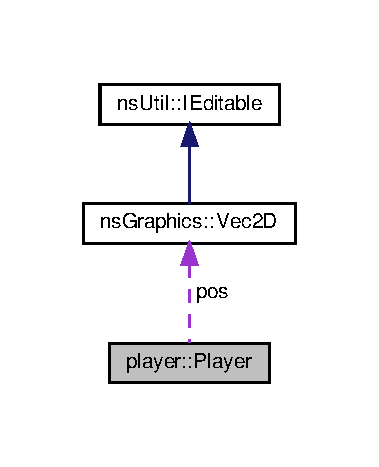
\includegraphics[width=182pt]{structplayer_1_1_player__coll__graph}
\end{center}
\end{figure}
\subsection*{Public Member Functions}
\begin{DoxyCompactItemize}
\item 
\hyperlink{structplayer_1_1_player_aea13d1e63bb4216dd7bb8ed925e9c058}{Player} (int entX, int entY, unsigned ent\+Id)
\begin{DoxyCompactList}\small\item\em Fonction constructeur de la struct \hyperlink{structplayer_1_1_player}{Player}. \end{DoxyCompactList}\item 
void \hyperlink{structplayer_1_1_player_a8a9a40b3c690c1edf7146b1f7132cd64}{update} ()
\begin{DoxyCompactList}\small\item\em Fonction de mise à jour du joueur en bloquant le tir. \end{DoxyCompactList}\item 
void \hyperlink{structplayer_1_1_player_a2a9b25a631e616ff91cb6ec815f9990a}{shoot} (unsigned from, unsigned to, std\+::vector$<$ \hyperlink{structtorpedo_1_1_torpedo}{torpedo\+::\+Torpedo} $>$ \&\hyperlink{multi_8cpp_a8d978ee3afff71f0b07f921403c2b403}{torpedos})
\begin{DoxyCompactList}\small\item\em Fonction qui ajoute une torpille allié au vecteur de torpilles et l\textquotesingle{}initialise. \end{DoxyCompactList}\item 
void \hyperlink{structplayer_1_1_player_a3f3f5a529fd56346902ca83672640294}{show} (\hyperlink{class_min_g_l}{Min\+GL} \&window)
\begin{DoxyCompactList}\small\item\em Permet d\textquotesingle{}afficher le joueur. \end{DoxyCompactList}\item 
void \hyperlink{structplayer_1_1_player_a26d56b47474cb89219f2aed8d92878d7}{show\+Life} (\hyperlink{class_min_g_l}{Min\+GL} \&window, \hyperlink{classns_graphics_1_1_vec2_d}{ns\+Graphics\+::\+Vec2D} \hyperlink{structplayer_1_1_player_aec9e16b6c6306f2ce5bfceec6210cb44}{pos})
\begin{DoxyCompactList}\small\item\em Affiche la vie du joueur. \end{DoxyCompactList}\end{DoxyCompactItemize}
\subsection*{Public Attributes}
\begin{DoxyCompactItemize}
\item 
\hyperlink{classns_graphics_1_1_vec2_d}{ns\+Graphics\+::\+Vec2D} \hyperlink{structplayer_1_1_player_aec9e16b6c6306f2ce5bfceec6210cb44}{pos}
\item 
std\+::vector$<$ unsigned long $>$ \hyperlink{structplayer_1_1_player_af4901794c6c932a6550973a88a446bac}{size}
\item 
int \hyperlink{structplayer_1_1_player_a5a59435adc56ae2dd435c815f01d1e4d}{life}
\item 
unsigned \hyperlink{structplayer_1_1_player_ae7306efe3b72df4b8ccce8f1612a4729}{shoot\+Limit}
\item 
unsigned \hyperlink{structplayer_1_1_player_a49a0c0e0b5bc07e6fa77cfecac963fb9}{shoot\+Count}
\item 
unsigned \hyperlink{structplayer_1_1_player_a40e8e3d989e0f045aca51d2e41239730}{id}
\item 
unsigned \hyperlink{structplayer_1_1_player_aec52e3bcc8710ab3c4d3d1f128f58e41}{score}
\item 
std\+::string \hyperlink{structplayer_1_1_player_a9294f29c7bcc3e5d44c4b7423cb2f13d}{pseudo}
\end{DoxyCompactItemize}


\subsection{Detailed Description}
Structure de joueur pour pouvoir les traiter en instance. 

Definition at line 29 of file player.\+h.



\subsection{Constructor \& Destructor Documentation}
\mbox{\Hypertarget{structplayer_1_1_player_aea13d1e63bb4216dd7bb8ed925e9c058}\label{structplayer_1_1_player_aea13d1e63bb4216dd7bb8ed925e9c058}} 
\index{player\+::\+Player@{player\+::\+Player}!Player@{Player}}
\index{Player@{Player}!player\+::\+Player@{player\+::\+Player}}
\subsubsection{\texorpdfstring{Player()}{Player()}}
{\footnotesize\ttfamily player\+::\+Player\+::\+Player (\begin{DoxyParamCaption}\item[{int}]{entX,  }\item[{int}]{entY,  }\item[{unsigned}]{ent\+Id }\end{DoxyParamCaption})}



Fonction constructeur de la struct \hyperlink{structplayer_1_1_player}{Player}. 


\begin{DoxyParams}[1]{Parameters}
\mbox{\tt in}  & {\em entX} & \+: position X \\
\hline
\mbox{\tt in}  & {\em entY} & \+: position Y \\
\hline
\mbox{\tt in}  & {\em ent\+Id} & \+: id du joueur \\
\hline
\end{DoxyParams}


Definition at line 17 of file player.\+cpp.



\subsection{Member Function Documentation}
\mbox{\Hypertarget{structplayer_1_1_player_a2a9b25a631e616ff91cb6ec815f9990a}\label{structplayer_1_1_player_a2a9b25a631e616ff91cb6ec815f9990a}} 
\index{player\+::\+Player@{player\+::\+Player}!shoot@{shoot}}
\index{shoot@{shoot}!player\+::\+Player@{player\+::\+Player}}
\subsubsection{\texorpdfstring{shoot()}{shoot()}}
{\footnotesize\ttfamily void player\+::\+Player\+::shoot (\begin{DoxyParamCaption}\item[{unsigned}]{from,  }\item[{unsigned}]{to,  }\item[{std\+::vector$<$ \hyperlink{structtorpedo_1_1_torpedo}{torpedo\+::\+Torpedo} $>$ \&}]{torpedos }\end{DoxyParamCaption})}



Fonction qui ajoute une torpille allié au vecteur de torpilles et l\textquotesingle{}initialise. 


\begin{DoxyParams}[1]{Parameters}
\mbox{\tt in}  & {\em from} & \+: quel joueur tir \\
\hline
\mbox{\tt in}  & {\em to} & \+: vers ou le joueur tir \\
\hline
\mbox{\tt in,out}  & {\em torpedos} & \+: vecteur de torpilles \\
\hline
\end{DoxyParams}


Definition at line 28 of file player.\+cpp.

\mbox{\Hypertarget{structplayer_1_1_player_a3f3f5a529fd56346902ca83672640294}\label{structplayer_1_1_player_a3f3f5a529fd56346902ca83672640294}} 
\index{player\+::\+Player@{player\+::\+Player}!show@{show}}
\index{show@{show}!player\+::\+Player@{player\+::\+Player}}
\subsubsection{\texorpdfstring{show()}{show()}}
{\footnotesize\ttfamily void player\+::\+Player\+::show (\begin{DoxyParamCaption}\item[{\hyperlink{class_min_g_l}{Min\+GL} \&}]{window }\end{DoxyParamCaption})}



Permet d\textquotesingle{}afficher le joueur. 


\begin{DoxyParams}[1]{Parameters}
\mbox{\tt in,out}  & {\em window} & \+: fenêtre de jeu \\
\hline
\end{DoxyParams}


Definition at line 44 of file player.\+cpp.

\mbox{\Hypertarget{structplayer_1_1_player_a26d56b47474cb89219f2aed8d92878d7}\label{structplayer_1_1_player_a26d56b47474cb89219f2aed8d92878d7}} 
\index{player\+::\+Player@{player\+::\+Player}!show\+Life@{show\+Life}}
\index{show\+Life@{show\+Life}!player\+::\+Player@{player\+::\+Player}}
\subsubsection{\texorpdfstring{show\+Life()}{showLife()}}
{\footnotesize\ttfamily void player\+::\+Player\+::show\+Life (\begin{DoxyParamCaption}\item[{\hyperlink{class_min_g_l}{Min\+GL} \&}]{window,  }\item[{\hyperlink{classns_graphics_1_1_vec2_d}{ns\+Graphics\+::\+Vec2D}}]{pos }\end{DoxyParamCaption})}



Affiche la vie du joueur. 


\begin{DoxyParams}{Parameters}
{\em window} & \+: La fenêtre de jeu \\
\hline
{\em pos} & \+: La position de oû sont affiché les vies \\
\hline
\end{DoxyParams}


Definition at line 48 of file player.\+cpp.

\mbox{\Hypertarget{structplayer_1_1_player_a8a9a40b3c690c1edf7146b1f7132cd64}\label{structplayer_1_1_player_a8a9a40b3c690c1edf7146b1f7132cd64}} 
\index{player\+::\+Player@{player\+::\+Player}!update@{update}}
\index{update@{update}!player\+::\+Player@{player\+::\+Player}}
\subsubsection{\texorpdfstring{update()}{update()}}
{\footnotesize\ttfamily void player\+::\+Player\+::update (\begin{DoxyParamCaption}{ }\end{DoxyParamCaption})}



Fonction de mise à jour du joueur en bloquant le tir. 



Definition at line 39 of file player.\+cpp.



\subsection{Member Data Documentation}
\mbox{\Hypertarget{structplayer_1_1_player_a40e8e3d989e0f045aca51d2e41239730}\label{structplayer_1_1_player_a40e8e3d989e0f045aca51d2e41239730}} 
\index{player\+::\+Player@{player\+::\+Player}!id@{id}}
\index{id@{id}!player\+::\+Player@{player\+::\+Player}}
\subsubsection{\texorpdfstring{id}{id}}
{\footnotesize\ttfamily unsigned player\+::\+Player\+::id}



Definition at line 37 of file player.\+h.

\mbox{\Hypertarget{structplayer_1_1_player_a5a59435adc56ae2dd435c815f01d1e4d}\label{structplayer_1_1_player_a5a59435adc56ae2dd435c815f01d1e4d}} 
\index{player\+::\+Player@{player\+::\+Player}!life@{life}}
\index{life@{life}!player\+::\+Player@{player\+::\+Player}}
\subsubsection{\texorpdfstring{life}{life}}
{\footnotesize\ttfamily int player\+::\+Player\+::life}



Definition at line 34 of file player.\+h.

\mbox{\Hypertarget{structplayer_1_1_player_aec9e16b6c6306f2ce5bfceec6210cb44}\label{structplayer_1_1_player_aec9e16b6c6306f2ce5bfceec6210cb44}} 
\index{player\+::\+Player@{player\+::\+Player}!pos@{pos}}
\index{pos@{pos}!player\+::\+Player@{player\+::\+Player}}
\subsubsection{\texorpdfstring{pos}{pos}}
{\footnotesize\ttfamily \hyperlink{classns_graphics_1_1_vec2_d}{ns\+Graphics\+::\+Vec2D} player\+::\+Player\+::pos}



Definition at line 32 of file player.\+h.

\mbox{\Hypertarget{structplayer_1_1_player_a9294f29c7bcc3e5d44c4b7423cb2f13d}\label{structplayer_1_1_player_a9294f29c7bcc3e5d44c4b7423cb2f13d}} 
\index{player\+::\+Player@{player\+::\+Player}!pseudo@{pseudo}}
\index{pseudo@{pseudo}!player\+::\+Player@{player\+::\+Player}}
\subsubsection{\texorpdfstring{pseudo}{pseudo}}
{\footnotesize\ttfamily std\+::string player\+::\+Player\+::pseudo}



Definition at line 39 of file player.\+h.

\mbox{\Hypertarget{structplayer_1_1_player_aec52e3bcc8710ab3c4d3d1f128f58e41}\label{structplayer_1_1_player_aec52e3bcc8710ab3c4d3d1f128f58e41}} 
\index{player\+::\+Player@{player\+::\+Player}!score@{score}}
\index{score@{score}!player\+::\+Player@{player\+::\+Player}}
\subsubsection{\texorpdfstring{score}{score}}
{\footnotesize\ttfamily unsigned player\+::\+Player\+::score}



Definition at line 38 of file player.\+h.

\mbox{\Hypertarget{structplayer_1_1_player_a49a0c0e0b5bc07e6fa77cfecac963fb9}\label{structplayer_1_1_player_a49a0c0e0b5bc07e6fa77cfecac963fb9}} 
\index{player\+::\+Player@{player\+::\+Player}!shoot\+Count@{shoot\+Count}}
\index{shoot\+Count@{shoot\+Count}!player\+::\+Player@{player\+::\+Player}}
\subsubsection{\texorpdfstring{shoot\+Count}{shootCount}}
{\footnotesize\ttfamily unsigned player\+::\+Player\+::shoot\+Count}



Definition at line 36 of file player.\+h.

\mbox{\Hypertarget{structplayer_1_1_player_ae7306efe3b72df4b8ccce8f1612a4729}\label{structplayer_1_1_player_ae7306efe3b72df4b8ccce8f1612a4729}} 
\index{player\+::\+Player@{player\+::\+Player}!shoot\+Limit@{shoot\+Limit}}
\index{shoot\+Limit@{shoot\+Limit}!player\+::\+Player@{player\+::\+Player}}
\subsubsection{\texorpdfstring{shoot\+Limit}{shootLimit}}
{\footnotesize\ttfamily unsigned player\+::\+Player\+::shoot\+Limit}



Definition at line 35 of file player.\+h.

\mbox{\Hypertarget{structplayer_1_1_player_af4901794c6c932a6550973a88a446bac}\label{structplayer_1_1_player_af4901794c6c932a6550973a88a446bac}} 
\index{player\+::\+Player@{player\+::\+Player}!size@{size}}
\index{size@{size}!player\+::\+Player@{player\+::\+Player}}
\subsubsection{\texorpdfstring{size}{size}}
{\footnotesize\ttfamily std\+::vector$<$unsigned long$>$ player\+::\+Player\+::size}



Definition at line 33 of file player.\+h.



The documentation for this struct was generated from the following files\+:\begin{DoxyCompactItemize}
\item 
libs/game/entities/\hyperlink{player_8h}{player.\+h}\item 
src/entities/\hyperlink{player_8cpp}{player.\+cpp}\end{DoxyCompactItemize}

\hypertarget{classns_shape_1_1_rectangle}{}\section{ns\+Shape\+:\+:Rectangle Class Reference}
\label{classns_shape_1_1_rectangle}\index{ns\+Shape\+::\+Rectangle@{ns\+Shape\+::\+Rectangle}}


Classe représentant un rectangle.  




{\ttfamily \#include $<$rectangle.\+h$>$}



Inheritance diagram for ns\+Shape\+:\+:Rectangle\+:
\nopagebreak
\begin{figure}[H]
\begin{center}
\leavevmode
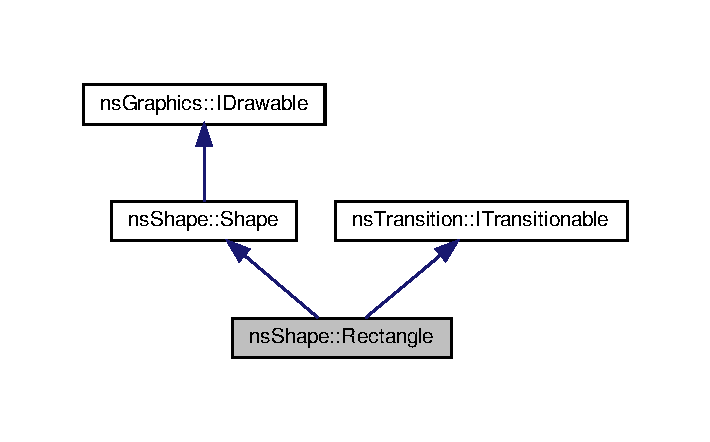
\includegraphics[width=341pt]{classns_shape_1_1_rectangle__inherit__graph}
\end{center}
\end{figure}


Collaboration diagram for ns\+Shape\+:\+:Rectangle\+:
\nopagebreak
\begin{figure}[H]
\begin{center}
\leavevmode
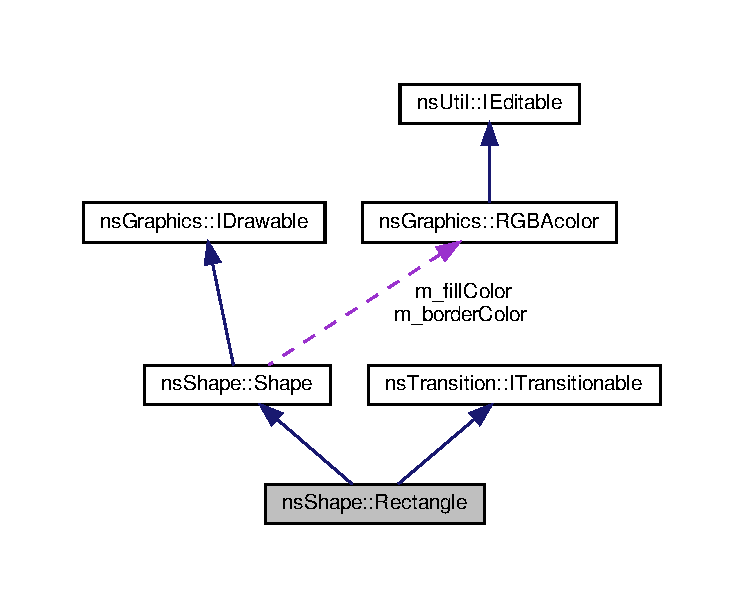
\includegraphics[width=350pt]{classns_shape_1_1_rectangle__coll__graph}
\end{center}
\end{figure}
\subsection*{Public Types}
\begin{DoxyCompactItemize}
\item 
enum \hyperlink{classns_shape_1_1_rectangle_a7c29d64ac1e4ed57a3d70b5616813247}{Transition\+Ids} \{ \newline
\hyperlink{classns_shape_1_1_rectangle_a7c29d64ac1e4ed57a3d70b5616813247a7711b3fc0ebda426d84aba567ef90797}{T\+R\+A\+N\+S\+I\+T\+I\+O\+N\+\_\+\+F\+I\+L\+L\+\_\+\+C\+O\+L\+O\+R\+\_\+\+R\+GB}, 
\hyperlink{classns_shape_1_1_rectangle_a7c29d64ac1e4ed57a3d70b5616813247a3162d563f05248a8a8e9f0ffed332ef0}{T\+R\+A\+N\+S\+I\+T\+I\+O\+N\+\_\+\+F\+I\+L\+L\+\_\+\+C\+O\+L\+O\+R\+\_\+\+A\+L\+P\+HA}, 
\hyperlink{classns_shape_1_1_rectangle_a7c29d64ac1e4ed57a3d70b5616813247a8ba797ba7b99e6952ab754191bf4e553}{T\+R\+A\+N\+S\+I\+T\+I\+O\+N\+\_\+\+B\+O\+R\+D\+E\+R\+\_\+\+C\+O\+L\+O\+R\+\_\+\+R\+GB}, 
\hyperlink{classns_shape_1_1_rectangle_a7c29d64ac1e4ed57a3d70b5616813247ad44045321ec0fd066d54f5a8f41fd947}{T\+R\+A\+N\+S\+I\+T\+I\+O\+N\+\_\+\+B\+O\+R\+D\+E\+R\+\_\+\+C\+O\+L\+O\+R\+\_\+\+A\+L\+P\+HA}, 
\newline
\hyperlink{classns_shape_1_1_rectangle_a7c29d64ac1e4ed57a3d70b5616813247a59d3d78acfe501ec8bed5b31ac8f4230}{T\+R\+A\+N\+S\+I\+T\+I\+O\+N\+\_\+\+F\+I\+R\+S\+T\+\_\+\+P\+O\+S\+I\+T\+I\+ON}, 
\hyperlink{classns_shape_1_1_rectangle_a7c29d64ac1e4ed57a3d70b5616813247a039bcc9b4d76cdb9e15debda929f41ef}{T\+R\+A\+N\+S\+I\+T\+I\+O\+N\+\_\+\+S\+E\+C\+O\+N\+D\+\_\+\+P\+O\+S\+I\+T\+I\+ON}
 \}\begin{DoxyCompactList}\small\item\em Transition\+Ids \+: Liste de toutes les transitions que cet élément peut exécuter. \end{DoxyCompactList}
\end{DoxyCompactItemize}
\subsection*{Public Member Functions}
\begin{DoxyCompactItemize}
\item 
\hyperlink{classns_shape_1_1_rectangle_a5d5e8052ba7c35001a30ccc7dad669e2}{Rectangle} (const \hyperlink{classns_graphics_1_1_vec2_d}{ns\+Graphics\+::\+Vec2D} \&first\+Position, const \hyperlink{classns_graphics_1_1_vec2_d}{ns\+Graphics\+::\+Vec2D} \&second\+Position, const \hyperlink{classns_graphics_1_1_r_g_b_acolor}{ns\+Graphics\+::\+R\+G\+B\+Acolor} \&fill\+Color, const \hyperlink{classns_graphics_1_1_r_g_b_acolor}{ns\+Graphics\+::\+R\+G\+B\+Acolor} \&border\+Color=\hyperlink{namespacens_graphics_ab2001ad03cceb2565849e04465618c1e}{ns\+Graphics\+::\+K\+Transparent})
\begin{DoxyCompactList}\small\item\em Constructeur pour la classe \hyperlink{classns_shape_1_1_rectangle}{Rectangle}. \end{DoxyCompactList}\item 
\hyperlink{classns_shape_1_1_rectangle_a0c1c16410fb0ee7345449d7bfc9b377b}{Rectangle} (const \hyperlink{classns_graphics_1_1_vec2_d}{ns\+Graphics\+::\+Vec2D} \&position, const unsigned \&width, const unsigned \&height, const \hyperlink{classns_graphics_1_1_r_g_b_acolor}{ns\+Graphics\+::\+R\+G\+B\+Acolor} \&fill\+Color, const \hyperlink{classns_graphics_1_1_r_g_b_acolor}{ns\+Graphics\+::\+R\+G\+B\+Acolor} \&border\+Color=\hyperlink{namespacens_graphics_ab2001ad03cceb2565849e04465618c1e}{ns\+Graphics\+::\+K\+Transparent})
\begin{DoxyCompactList}\small\item\em Constructeur pour la classe \hyperlink{classns_shape_1_1_rectangle}{Rectangle}. \end{DoxyCompactList}\item 
virtual \hyperlink{classns_shape_1_1_rectangle_a8c5a662392d6ff84a852c4f70e8b1d1d}{$\sim$\+Rectangle} () override=default
\item 
virtual void \hyperlink{classns_shape_1_1_rectangle_acbe8ed9e23b67090e7638563f2593735}{draw} (\hyperlink{class_min_g_l}{Min\+GL} \&window) const override
\begin{DoxyCompactList}\small\item\em Fonction pour afficher l\textquotesingle{}objet. \end{DoxyCompactList}\item 
virtual void \hyperlink{classns_shape_1_1_rectangle_a379d73a44d0601a12f26d4867e4246d8}{get\+Values} (const int \&id, std\+::vector$<$ float $>$ \&values) override
\begin{DoxyCompactList}\small\item\em Récupère des valeurs dans un vecteur de float pour l\textquotesingle{}ID spécifié \end{DoxyCompactList}\item 
virtual void \hyperlink{classns_shape_1_1_rectangle_a9fcdc9a8adbc91cd2613a0d50058f829}{set\+Values} (const int \&id, const std\+::vector$<$ float $>$ \&values) override
\begin{DoxyCompactList}\small\item\em Définit les nouvelles valeurs pour l\textquotesingle{}ID spécifié \end{DoxyCompactList}\item 
\hyperlink{classns_shape_1_1_rectangle}{Rectangle} \hyperlink{classns_shape_1_1_rectangle_ac86de3402279c3ad0bf6b3869f8e2613}{operator+} (const \hyperlink{classns_graphics_1_1_vec2_d}{ns\+Graphics\+::\+Vec2D} \&position) const
\begin{DoxyCompactList}\small\item\em Opérateur de décalage. \end{DoxyCompactList}\item 
\hyperlink{classns_shape_1_1_rectangle}{Rectangle} \hyperlink{classns_shape_1_1_rectangle_af7cbf6d75b4bc8fc718d17177abdd344}{operator$\ast$} (const float \&f) const
\begin{DoxyCompactList}\small\item\em Opérateur de réduction. \end{DoxyCompactList}\item 
const \hyperlink{classns_graphics_1_1_vec2_d}{ns\+Graphics\+::\+Vec2D} \& \hyperlink{classns_shape_1_1_rectangle_a42c38f27b247f6a411a9d1a8de5ceaa4}{get\+First\+Position} () const
\begin{DoxyCompactList}\small\item\em Récupère la position du coin haut-\/gauche du rectangle. \end{DoxyCompactList}\item 
void \hyperlink{classns_shape_1_1_rectangle_ae6c787fad1bc33f5a4adf8a697a9a581}{set\+First\+Position} (const \hyperlink{classns_graphics_1_1_vec2_d}{ns\+Graphics\+::\+Vec2D} \&first\+Position)
\begin{DoxyCompactList}\small\item\em Définit la nouvelle position du coin haut-\/gauche du rectangle. \end{DoxyCompactList}\item 
const \hyperlink{classns_graphics_1_1_vec2_d}{ns\+Graphics\+::\+Vec2D} \& \hyperlink{classns_shape_1_1_rectangle_a276bce487fbd9514fcf8e558382d0276}{get\+Second\+Position} () const
\begin{DoxyCompactList}\small\item\em Récupère la position du coin bas-\/droit du rectangle. \end{DoxyCompactList}\item 
void \hyperlink{classns_shape_1_1_rectangle_ada11c6f627048c51dce9544bff758db4}{set\+Second\+Position} (const \hyperlink{classns_graphics_1_1_vec2_d}{ns\+Graphics\+::\+Vec2D} \&second\+Position)
\begin{DoxyCompactList}\small\item\em Définit la nouvelle position du coin bas-\/droit du rectangle. \end{DoxyCompactList}\end{DoxyCompactItemize}
\subsection*{Additional Inherited Members}


\subsection{Detailed Description}
Classe représentant un rectangle. 

Definition at line 25 of file rectangle.\+h.



\subsection{Member Enumeration Documentation}
\mbox{\Hypertarget{classns_shape_1_1_rectangle_a7c29d64ac1e4ed57a3d70b5616813247}\label{classns_shape_1_1_rectangle_a7c29d64ac1e4ed57a3d70b5616813247}} 
\index{ns\+Shape\+::\+Rectangle@{ns\+Shape\+::\+Rectangle}!Transition\+Ids@{Transition\+Ids}}
\index{Transition\+Ids@{Transition\+Ids}!ns\+Shape\+::\+Rectangle@{ns\+Shape\+::\+Rectangle}}
\subsubsection{\texorpdfstring{Transition\+Ids}{TransitionIds}}
{\footnotesize\ttfamily enum \hyperlink{classns_shape_1_1_rectangle_a7c29d64ac1e4ed57a3d70b5616813247}{ns\+Shape\+::\+Rectangle\+::\+Transition\+Ids}}



Transition\+Ids \+: Liste de toutes les transitions que cet élément peut exécuter. 

\begin{DoxyEnumFields}{Enumerator}
\raisebox{\heightof{T}}[0pt][0pt]{\index{T\+R\+A\+N\+S\+I\+T\+I\+O\+N\+\_\+\+F\+I\+L\+L\+\_\+\+C\+O\+L\+O\+R\+\_\+\+R\+GB@{T\+R\+A\+N\+S\+I\+T\+I\+O\+N\+\_\+\+F\+I\+L\+L\+\_\+\+C\+O\+L\+O\+R\+\_\+\+R\+GB}!ns\+Shape\+::\+Rectangle@{ns\+Shape\+::\+Rectangle}}\index{ns\+Shape\+::\+Rectangle@{ns\+Shape\+::\+Rectangle}!T\+R\+A\+N\+S\+I\+T\+I\+O\+N\+\_\+\+F\+I\+L\+L\+\_\+\+C\+O\+L\+O\+R\+\_\+\+R\+GB@{T\+R\+A\+N\+S\+I\+T\+I\+O\+N\+\_\+\+F\+I\+L\+L\+\_\+\+C\+O\+L\+O\+R\+\_\+\+R\+GB}}}\mbox{\Hypertarget{classns_shape_1_1_rectangle_a7c29d64ac1e4ed57a3d70b5616813247a7711b3fc0ebda426d84aba567ef90797}\label{classns_shape_1_1_rectangle_a7c29d64ac1e4ed57a3d70b5616813247a7711b3fc0ebda426d84aba567ef90797}} 
T\+R\+A\+N\+S\+I\+T\+I\+O\+N\+\_\+\+F\+I\+L\+L\+\_\+\+C\+O\+L\+O\+R\+\_\+\+R\+GB&Transition pour la couleur de remplissage \\
\hline

\raisebox{\heightof{T}}[0pt][0pt]{\index{T\+R\+A\+N\+S\+I\+T\+I\+O\+N\+\_\+\+F\+I\+L\+L\+\_\+\+C\+O\+L\+O\+R\+\_\+\+A\+L\+P\+HA@{T\+R\+A\+N\+S\+I\+T\+I\+O\+N\+\_\+\+F\+I\+L\+L\+\_\+\+C\+O\+L\+O\+R\+\_\+\+A\+L\+P\+HA}!ns\+Shape\+::\+Rectangle@{ns\+Shape\+::\+Rectangle}}\index{ns\+Shape\+::\+Rectangle@{ns\+Shape\+::\+Rectangle}!T\+R\+A\+N\+S\+I\+T\+I\+O\+N\+\_\+\+F\+I\+L\+L\+\_\+\+C\+O\+L\+O\+R\+\_\+\+A\+L\+P\+HA@{T\+R\+A\+N\+S\+I\+T\+I\+O\+N\+\_\+\+F\+I\+L\+L\+\_\+\+C\+O\+L\+O\+R\+\_\+\+A\+L\+P\+HA}}}\mbox{\Hypertarget{classns_shape_1_1_rectangle_a7c29d64ac1e4ed57a3d70b5616813247a3162d563f05248a8a8e9f0ffed332ef0}\label{classns_shape_1_1_rectangle_a7c29d64ac1e4ed57a3d70b5616813247a3162d563f05248a8a8e9f0ffed332ef0}} 
T\+R\+A\+N\+S\+I\+T\+I\+O\+N\+\_\+\+F\+I\+L\+L\+\_\+\+C\+O\+L\+O\+R\+\_\+\+A\+L\+P\+HA&Transition pour la transparence de remplissage \\
\hline

\raisebox{\heightof{T}}[0pt][0pt]{\index{T\+R\+A\+N\+S\+I\+T\+I\+O\+N\+\_\+\+B\+O\+R\+D\+E\+R\+\_\+\+C\+O\+L\+O\+R\+\_\+\+R\+GB@{T\+R\+A\+N\+S\+I\+T\+I\+O\+N\+\_\+\+B\+O\+R\+D\+E\+R\+\_\+\+C\+O\+L\+O\+R\+\_\+\+R\+GB}!ns\+Shape\+::\+Rectangle@{ns\+Shape\+::\+Rectangle}}\index{ns\+Shape\+::\+Rectangle@{ns\+Shape\+::\+Rectangle}!T\+R\+A\+N\+S\+I\+T\+I\+O\+N\+\_\+\+B\+O\+R\+D\+E\+R\+\_\+\+C\+O\+L\+O\+R\+\_\+\+R\+GB@{T\+R\+A\+N\+S\+I\+T\+I\+O\+N\+\_\+\+B\+O\+R\+D\+E\+R\+\_\+\+C\+O\+L\+O\+R\+\_\+\+R\+GB}}}\mbox{\Hypertarget{classns_shape_1_1_rectangle_a7c29d64ac1e4ed57a3d70b5616813247a8ba797ba7b99e6952ab754191bf4e553}\label{classns_shape_1_1_rectangle_a7c29d64ac1e4ed57a3d70b5616813247a8ba797ba7b99e6952ab754191bf4e553}} 
T\+R\+A\+N\+S\+I\+T\+I\+O\+N\+\_\+\+B\+O\+R\+D\+E\+R\+\_\+\+C\+O\+L\+O\+R\+\_\+\+R\+GB&Transition pour la couleur de bord \\
\hline

\raisebox{\heightof{T}}[0pt][0pt]{\index{T\+R\+A\+N\+S\+I\+T\+I\+O\+N\+\_\+\+B\+O\+R\+D\+E\+R\+\_\+\+C\+O\+L\+O\+R\+\_\+\+A\+L\+P\+HA@{T\+R\+A\+N\+S\+I\+T\+I\+O\+N\+\_\+\+B\+O\+R\+D\+E\+R\+\_\+\+C\+O\+L\+O\+R\+\_\+\+A\+L\+P\+HA}!ns\+Shape\+::\+Rectangle@{ns\+Shape\+::\+Rectangle}}\index{ns\+Shape\+::\+Rectangle@{ns\+Shape\+::\+Rectangle}!T\+R\+A\+N\+S\+I\+T\+I\+O\+N\+\_\+\+B\+O\+R\+D\+E\+R\+\_\+\+C\+O\+L\+O\+R\+\_\+\+A\+L\+P\+HA@{T\+R\+A\+N\+S\+I\+T\+I\+O\+N\+\_\+\+B\+O\+R\+D\+E\+R\+\_\+\+C\+O\+L\+O\+R\+\_\+\+A\+L\+P\+HA}}}\mbox{\Hypertarget{classns_shape_1_1_rectangle_a7c29d64ac1e4ed57a3d70b5616813247ad44045321ec0fd066d54f5a8f41fd947}\label{classns_shape_1_1_rectangle_a7c29d64ac1e4ed57a3d70b5616813247ad44045321ec0fd066d54f5a8f41fd947}} 
T\+R\+A\+N\+S\+I\+T\+I\+O\+N\+\_\+\+B\+O\+R\+D\+E\+R\+\_\+\+C\+O\+L\+O\+R\+\_\+\+A\+L\+P\+HA&Transition pour la transparence de bord \\
\hline

\raisebox{\heightof{T}}[0pt][0pt]{\index{T\+R\+A\+N\+S\+I\+T\+I\+O\+N\+\_\+\+F\+I\+R\+S\+T\+\_\+\+P\+O\+S\+I\+T\+I\+ON@{T\+R\+A\+N\+S\+I\+T\+I\+O\+N\+\_\+\+F\+I\+R\+S\+T\+\_\+\+P\+O\+S\+I\+T\+I\+ON}!ns\+Shape\+::\+Rectangle@{ns\+Shape\+::\+Rectangle}}\index{ns\+Shape\+::\+Rectangle@{ns\+Shape\+::\+Rectangle}!T\+R\+A\+N\+S\+I\+T\+I\+O\+N\+\_\+\+F\+I\+R\+S\+T\+\_\+\+P\+O\+S\+I\+T\+I\+ON@{T\+R\+A\+N\+S\+I\+T\+I\+O\+N\+\_\+\+F\+I\+R\+S\+T\+\_\+\+P\+O\+S\+I\+T\+I\+ON}}}\mbox{\Hypertarget{classns_shape_1_1_rectangle_a7c29d64ac1e4ed57a3d70b5616813247a59d3d78acfe501ec8bed5b31ac8f4230}\label{classns_shape_1_1_rectangle_a7c29d64ac1e4ed57a3d70b5616813247a59d3d78acfe501ec8bed5b31ac8f4230}} 
T\+R\+A\+N\+S\+I\+T\+I\+O\+N\+\_\+\+F\+I\+R\+S\+T\+\_\+\+P\+O\+S\+I\+T\+I\+ON&Transition pour la position du coin haut-\/gauche \\
\hline

\raisebox{\heightof{T}}[0pt][0pt]{\index{T\+R\+A\+N\+S\+I\+T\+I\+O\+N\+\_\+\+S\+E\+C\+O\+N\+D\+\_\+\+P\+O\+S\+I\+T\+I\+ON@{T\+R\+A\+N\+S\+I\+T\+I\+O\+N\+\_\+\+S\+E\+C\+O\+N\+D\+\_\+\+P\+O\+S\+I\+T\+I\+ON}!ns\+Shape\+::\+Rectangle@{ns\+Shape\+::\+Rectangle}}\index{ns\+Shape\+::\+Rectangle@{ns\+Shape\+::\+Rectangle}!T\+R\+A\+N\+S\+I\+T\+I\+O\+N\+\_\+\+S\+E\+C\+O\+N\+D\+\_\+\+P\+O\+S\+I\+T\+I\+ON@{T\+R\+A\+N\+S\+I\+T\+I\+O\+N\+\_\+\+S\+E\+C\+O\+N\+D\+\_\+\+P\+O\+S\+I\+T\+I\+ON}}}\mbox{\Hypertarget{classns_shape_1_1_rectangle_a7c29d64ac1e4ed57a3d70b5616813247a039bcc9b4d76cdb9e15debda929f41ef}\label{classns_shape_1_1_rectangle_a7c29d64ac1e4ed57a3d70b5616813247a039bcc9b4d76cdb9e15debda929f41ef}} 
T\+R\+A\+N\+S\+I\+T\+I\+O\+N\+\_\+\+S\+E\+C\+O\+N\+D\+\_\+\+P\+O\+S\+I\+T\+I\+ON&Transition pour la position du coin bas-\/droit \\
\hline

\end{DoxyEnumFields}


Definition at line 32 of file rectangle.\+h.



\subsection{Constructor \& Destructor Documentation}
\mbox{\Hypertarget{classns_shape_1_1_rectangle_a5d5e8052ba7c35001a30ccc7dad669e2}\label{classns_shape_1_1_rectangle_a5d5e8052ba7c35001a30ccc7dad669e2}} 
\index{ns\+Shape\+::\+Rectangle@{ns\+Shape\+::\+Rectangle}!Rectangle@{Rectangle}}
\index{Rectangle@{Rectangle}!ns\+Shape\+::\+Rectangle@{ns\+Shape\+::\+Rectangle}}
\subsubsection{\texorpdfstring{Rectangle()}{Rectangle()}\hspace{0.1cm}{\footnotesize\ttfamily [1/2]}}
{\footnotesize\ttfamily ns\+Shape\+::\+Rectangle\+::\+Rectangle (\begin{DoxyParamCaption}\item[{const \hyperlink{classns_graphics_1_1_vec2_d}{ns\+Graphics\+::\+Vec2D} \&}]{first\+Position,  }\item[{const \hyperlink{classns_graphics_1_1_vec2_d}{ns\+Graphics\+::\+Vec2D} \&}]{second\+Position,  }\item[{const \hyperlink{classns_graphics_1_1_r_g_b_acolor}{ns\+Graphics\+::\+R\+G\+B\+Acolor} \&}]{fill\+Color,  }\item[{const \hyperlink{classns_graphics_1_1_r_g_b_acolor}{ns\+Graphics\+::\+R\+G\+B\+Acolor} \&}]{border\+Color = {\ttfamily \hyperlink{namespacens_graphics_ab2001ad03cceb2565849e04465618c1e}{ns\+Graphics\+::\+K\+Transparent}} }\end{DoxyParamCaption})}



Constructeur pour la classe \hyperlink{classns_shape_1_1_rectangle}{Rectangle}. 


\begin{DoxyParams}[1]{Parameters}
\mbox{\tt in}  & {\em first\+Position} & \+: Position du coin haut-\/gauche \\
\hline
\mbox{\tt in}  & {\em second\+Position} & \+: Position du coin bas-\/droit \\
\hline
\mbox{\tt in}  & {\em fill\+Color} & \+: Couleur de remplissage \\
\hline
\mbox{\tt in}  & {\em border\+Color} & \+: Couleur de bord \\
\hline
\end{DoxyParams}
\mbox{\Hypertarget{classns_shape_1_1_rectangle_a0c1c16410fb0ee7345449d7bfc9b377b}\label{classns_shape_1_1_rectangle_a0c1c16410fb0ee7345449d7bfc9b377b}} 
\index{ns\+Shape\+::\+Rectangle@{ns\+Shape\+::\+Rectangle}!Rectangle@{Rectangle}}
\index{Rectangle@{Rectangle}!ns\+Shape\+::\+Rectangle@{ns\+Shape\+::\+Rectangle}}
\subsubsection{\texorpdfstring{Rectangle()}{Rectangle()}\hspace{0.1cm}{\footnotesize\ttfamily [2/2]}}
{\footnotesize\ttfamily ns\+Shape\+::\+Rectangle\+::\+Rectangle (\begin{DoxyParamCaption}\item[{const \hyperlink{classns_graphics_1_1_vec2_d}{ns\+Graphics\+::\+Vec2D} \&}]{position,  }\item[{const unsigned \&}]{width,  }\item[{const unsigned \&}]{height,  }\item[{const \hyperlink{classns_graphics_1_1_r_g_b_acolor}{ns\+Graphics\+::\+R\+G\+B\+Acolor} \&}]{fill\+Color,  }\item[{const \hyperlink{classns_graphics_1_1_r_g_b_acolor}{ns\+Graphics\+::\+R\+G\+B\+Acolor} \&}]{border\+Color = {\ttfamily \hyperlink{namespacens_graphics_ab2001ad03cceb2565849e04465618c1e}{ns\+Graphics\+::\+K\+Transparent}} }\end{DoxyParamCaption})}



Constructeur pour la classe \hyperlink{classns_shape_1_1_rectangle}{Rectangle}. 


\begin{DoxyParams}[1]{Parameters}
\mbox{\tt in}  & {\em position} & \+: Position du coin haut-\/gauche \\
\hline
\mbox{\tt in}  & {\em width} & \+: Largeur du rectangle \\
\hline
\mbox{\tt in}  & {\em height} & \+: Hauteur du rectangle \\
\hline
\mbox{\tt in}  & {\em fill\+Color} & \+: Couleur de remplissage \\
\hline
\mbox{\tt in}  & {\em border\+Color} & \+: Couleur de bord \\
\hline
\end{DoxyParams}
\mbox{\Hypertarget{classns_shape_1_1_rectangle_a8c5a662392d6ff84a852c4f70e8b1d1d}\label{classns_shape_1_1_rectangle_a8c5a662392d6ff84a852c4f70e8b1d1d}} 
\index{ns\+Shape\+::\+Rectangle@{ns\+Shape\+::\+Rectangle}!````~Rectangle@{$\sim$\+Rectangle}}
\index{````~Rectangle@{$\sim$\+Rectangle}!ns\+Shape\+::\+Rectangle@{ns\+Shape\+::\+Rectangle}}
\subsubsection{\texorpdfstring{$\sim$\+Rectangle()}{~Rectangle()}}
{\footnotesize\ttfamily virtual ns\+Shape\+::\+Rectangle\+::$\sim$\+Rectangle (\begin{DoxyParamCaption}{ }\end{DoxyParamCaption})\hspace{0.3cm}{\ttfamily [override]}, {\ttfamily [virtual]}, {\ttfamily [default]}}



\subsection{Member Function Documentation}
\mbox{\Hypertarget{classns_shape_1_1_rectangle_acbe8ed9e23b67090e7638563f2593735}\label{classns_shape_1_1_rectangle_acbe8ed9e23b67090e7638563f2593735}} 
\index{ns\+Shape\+::\+Rectangle@{ns\+Shape\+::\+Rectangle}!draw@{draw}}
\index{draw@{draw}!ns\+Shape\+::\+Rectangle@{ns\+Shape\+::\+Rectangle}}
\subsubsection{\texorpdfstring{draw()}{draw()}}
{\footnotesize\ttfamily virtual void ns\+Shape\+::\+Rectangle\+::draw (\begin{DoxyParamCaption}\item[{\hyperlink{class_min_g_l}{Min\+GL} \&}]{window }\end{DoxyParamCaption}) const\hspace{0.3cm}{\ttfamily [override]}, {\ttfamily [virtual]}}



Fonction pour afficher l\textquotesingle{}objet. 



Implements \hyperlink{classns_graphics_1_1_i_drawable_abed8a61e1d507d31e76f0891f3bf9c51}{ns\+Graphics\+::\+I\+Drawable}.

\mbox{\Hypertarget{classns_shape_1_1_rectangle_a42c38f27b247f6a411a9d1a8de5ceaa4}\label{classns_shape_1_1_rectangle_a42c38f27b247f6a411a9d1a8de5ceaa4}} 
\index{ns\+Shape\+::\+Rectangle@{ns\+Shape\+::\+Rectangle}!get\+First\+Position@{get\+First\+Position}}
\index{get\+First\+Position@{get\+First\+Position}!ns\+Shape\+::\+Rectangle@{ns\+Shape\+::\+Rectangle}}
\subsubsection{\texorpdfstring{get\+First\+Position()}{getFirstPosition()}}
{\footnotesize\ttfamily const \hyperlink{classns_graphics_1_1_vec2_d}{ns\+Graphics\+::\+Vec2D} \& ns\+Shape\+::\+Rectangle\+::get\+First\+Position (\begin{DoxyParamCaption}{ }\end{DoxyParamCaption}) const}



Récupère la position du coin haut-\/gauche du rectangle. 

\mbox{\Hypertarget{classns_shape_1_1_rectangle_a276bce487fbd9514fcf8e558382d0276}\label{classns_shape_1_1_rectangle_a276bce487fbd9514fcf8e558382d0276}} 
\index{ns\+Shape\+::\+Rectangle@{ns\+Shape\+::\+Rectangle}!get\+Second\+Position@{get\+Second\+Position}}
\index{get\+Second\+Position@{get\+Second\+Position}!ns\+Shape\+::\+Rectangle@{ns\+Shape\+::\+Rectangle}}
\subsubsection{\texorpdfstring{get\+Second\+Position()}{getSecondPosition()}}
{\footnotesize\ttfamily const \hyperlink{classns_graphics_1_1_vec2_d}{ns\+Graphics\+::\+Vec2D} \& ns\+Shape\+::\+Rectangle\+::get\+Second\+Position (\begin{DoxyParamCaption}{ }\end{DoxyParamCaption}) const}



Récupère la position du coin bas-\/droit du rectangle. 

\mbox{\Hypertarget{classns_shape_1_1_rectangle_a379d73a44d0601a12f26d4867e4246d8}\label{classns_shape_1_1_rectangle_a379d73a44d0601a12f26d4867e4246d8}} 
\index{ns\+Shape\+::\+Rectangle@{ns\+Shape\+::\+Rectangle}!get\+Values@{get\+Values}}
\index{get\+Values@{get\+Values}!ns\+Shape\+::\+Rectangle@{ns\+Shape\+::\+Rectangle}}
\subsubsection{\texorpdfstring{get\+Values()}{getValues()}}
{\footnotesize\ttfamily virtual void ns\+Shape\+::\+Rectangle\+::get\+Values (\begin{DoxyParamCaption}\item[{const int \&}]{id,  }\item[{std\+::vector$<$ float $>$ \&}]{values }\end{DoxyParamCaption})\hspace{0.3cm}{\ttfamily [override]}, {\ttfamily [virtual]}}



Récupère des valeurs dans un vecteur de float pour l\textquotesingle{}ID spécifié 


\begin{DoxyParams}[1]{Parameters}
\mbox{\tt in}  & {\em id} & ID des valeurs a récupérer \\
\hline
\mbox{\tt in,out}  & {\em values} & Vecteur de valeurs a peupler \\
\hline
\end{DoxyParams}


Implements \hyperlink{classns_transition_1_1_i_transitionable_a5871a16fd47c1e5c8bacdd5da8597ed9}{ns\+Transition\+::\+I\+Transitionable}.

\mbox{\Hypertarget{classns_shape_1_1_rectangle_af7cbf6d75b4bc8fc718d17177abdd344}\label{classns_shape_1_1_rectangle_af7cbf6d75b4bc8fc718d17177abdd344}} 
\index{ns\+Shape\+::\+Rectangle@{ns\+Shape\+::\+Rectangle}!operator$\ast$@{operator$\ast$}}
\index{operator$\ast$@{operator$\ast$}!ns\+Shape\+::\+Rectangle@{ns\+Shape\+::\+Rectangle}}
\subsubsection{\texorpdfstring{operator$\ast$()}{operator*()}}
{\footnotesize\ttfamily \hyperlink{classns_shape_1_1_rectangle}{Rectangle} ns\+Shape\+::\+Rectangle\+::operator$\ast$ (\begin{DoxyParamCaption}\item[{const float \&}]{f }\end{DoxyParamCaption}) const}



Opérateur de réduction. 


\begin{DoxyParams}[1]{Parameters}
\mbox{\tt in}  & {\em f} & \+: Nombre avec lequel multiplier la position actuelle \\
\hline
\end{DoxyParams}
\mbox{\Hypertarget{classns_shape_1_1_rectangle_ac86de3402279c3ad0bf6b3869f8e2613}\label{classns_shape_1_1_rectangle_ac86de3402279c3ad0bf6b3869f8e2613}} 
\index{ns\+Shape\+::\+Rectangle@{ns\+Shape\+::\+Rectangle}!operator+@{operator+}}
\index{operator+@{operator+}!ns\+Shape\+::\+Rectangle@{ns\+Shape\+::\+Rectangle}}
\subsubsection{\texorpdfstring{operator+()}{operator+()}}
{\footnotesize\ttfamily \hyperlink{classns_shape_1_1_rectangle}{Rectangle} ns\+Shape\+::\+Rectangle\+::operator+ (\begin{DoxyParamCaption}\item[{const \hyperlink{classns_graphics_1_1_vec2_d}{ns\+Graphics\+::\+Vec2D} \&}]{position }\end{DoxyParamCaption}) const}



Opérateur de décalage. 


\begin{DoxyParams}[1]{Parameters}
\mbox{\tt in}  & {\em position} & \+: Position a additionner \\
\hline
\end{DoxyParams}
\mbox{\Hypertarget{classns_shape_1_1_rectangle_ae6c787fad1bc33f5a4adf8a697a9a581}\label{classns_shape_1_1_rectangle_ae6c787fad1bc33f5a4adf8a697a9a581}} 
\index{ns\+Shape\+::\+Rectangle@{ns\+Shape\+::\+Rectangle}!set\+First\+Position@{set\+First\+Position}}
\index{set\+First\+Position@{set\+First\+Position}!ns\+Shape\+::\+Rectangle@{ns\+Shape\+::\+Rectangle}}
\subsubsection{\texorpdfstring{set\+First\+Position()}{setFirstPosition()}}
{\footnotesize\ttfamily void ns\+Shape\+::\+Rectangle\+::set\+First\+Position (\begin{DoxyParamCaption}\item[{const \hyperlink{classns_graphics_1_1_vec2_d}{ns\+Graphics\+::\+Vec2D} \&}]{first\+Position }\end{DoxyParamCaption})}



Définit la nouvelle position du coin haut-\/gauche du rectangle. 


\begin{DoxyParams}[1]{Parameters}
\mbox{\tt in}  & {\em first\+Position} & \+: Nouvelle position du coin haut-\/gauche \\
\hline
\end{DoxyParams}
\mbox{\Hypertarget{classns_shape_1_1_rectangle_ada11c6f627048c51dce9544bff758db4}\label{classns_shape_1_1_rectangle_ada11c6f627048c51dce9544bff758db4}} 
\index{ns\+Shape\+::\+Rectangle@{ns\+Shape\+::\+Rectangle}!set\+Second\+Position@{set\+Second\+Position}}
\index{set\+Second\+Position@{set\+Second\+Position}!ns\+Shape\+::\+Rectangle@{ns\+Shape\+::\+Rectangle}}
\subsubsection{\texorpdfstring{set\+Second\+Position()}{setSecondPosition()}}
{\footnotesize\ttfamily void ns\+Shape\+::\+Rectangle\+::set\+Second\+Position (\begin{DoxyParamCaption}\item[{const \hyperlink{classns_graphics_1_1_vec2_d}{ns\+Graphics\+::\+Vec2D} \&}]{second\+Position }\end{DoxyParamCaption})}



Définit la nouvelle position du coin bas-\/droit du rectangle. 


\begin{DoxyParams}[1]{Parameters}
\mbox{\tt in}  & {\em second\+Position} & \+: Nouvelle position du coin bas-\/droit \\
\hline
\end{DoxyParams}
\mbox{\Hypertarget{classns_shape_1_1_rectangle_a9fcdc9a8adbc91cd2613a0d50058f829}\label{classns_shape_1_1_rectangle_a9fcdc9a8adbc91cd2613a0d50058f829}} 
\index{ns\+Shape\+::\+Rectangle@{ns\+Shape\+::\+Rectangle}!set\+Values@{set\+Values}}
\index{set\+Values@{set\+Values}!ns\+Shape\+::\+Rectangle@{ns\+Shape\+::\+Rectangle}}
\subsubsection{\texorpdfstring{set\+Values()}{setValues()}}
{\footnotesize\ttfamily virtual void ns\+Shape\+::\+Rectangle\+::set\+Values (\begin{DoxyParamCaption}\item[{const int \&}]{id,  }\item[{const std\+::vector$<$ float $>$ \&}]{values }\end{DoxyParamCaption})\hspace{0.3cm}{\ttfamily [override]}, {\ttfamily [virtual]}}



Définit les nouvelles valeurs pour l\textquotesingle{}ID spécifié 


\begin{DoxyParams}[1]{Parameters}
\mbox{\tt in}  & {\em id} & ID des valeurs a définir \\
\hline
\mbox{\tt in}  & {\em values} & Vecteur des nouvelles valeurs a appliquer \\
\hline
\end{DoxyParams}


Implements \hyperlink{classns_transition_1_1_i_transitionable_ade37d29f7f2ca4890ed0e2e64d033197}{ns\+Transition\+::\+I\+Transitionable}.



The documentation for this class was generated from the following file\+:\begin{DoxyCompactItemize}
\item 
libs/mingl/shape/\hyperlink{rectangle_8h}{rectangle.\+h}\end{DoxyCompactItemize}

\hypertarget{classns_graphics_1_1_r_g_b_acolor}{}\section{ns\+Graphics\+:\+:R\+G\+B\+Acolor Class Reference}
\label{classns_graphics_1_1_r_g_b_acolor}\index{ns\+Graphics\+::\+R\+G\+B\+Acolor@{ns\+Graphics\+::\+R\+G\+B\+Acolor}}


Classe représentant un couleur R\+G\+B\+A8888.  




{\ttfamily \#include $<$rgbacolor.\+h$>$}



Inheritance diagram for ns\+Graphics\+:\+:R\+G\+B\+Acolor\+:
\nopagebreak
\begin{figure}[H]
\begin{center}
\leavevmode
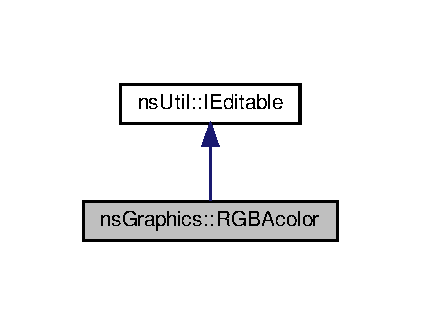
\includegraphics[width=202pt]{classns_graphics_1_1_r_g_b_acolor__inherit__graph}
\end{center}
\end{figure}


Collaboration diagram for ns\+Graphics\+:\+:R\+G\+B\+Acolor\+:
\nopagebreak
\begin{figure}[H]
\begin{center}
\leavevmode
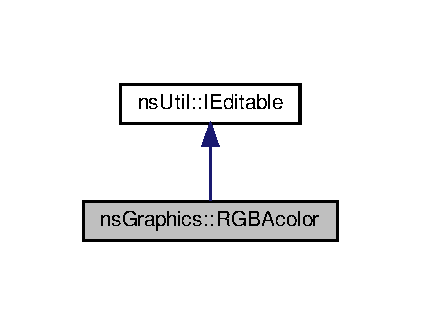
\includegraphics[width=202pt]{classns_graphics_1_1_r_g_b_acolor__coll__graph}
\end{center}
\end{figure}
\subsection*{Public Member Functions}
\begin{DoxyCompactItemize}
\item 
\hyperlink{classns_graphics_1_1_r_g_b_acolor_a6f91976b2d83414329608564615f27b1}{R\+G\+B\+Acolor} (const G\+Lubyte \&red=0, const G\+Lubyte \&green=0, const G\+Lubyte \&blue=0, const G\+Lubyte \&\hyperlink{get_pseudo_8cpp_a91dd017bd061f2dac37ce9b6e37cb360}{alpha}=255)
\begin{DoxyCompactList}\small\item\em Constructeur pour la classe \hyperlink{classns_graphics_1_1_r_g_b_acolor}{R\+G\+B\+Acolor}. \end{DoxyCompactList}\item 
virtual \hyperlink{classns_graphics_1_1_r_g_b_acolor_a229faf986de81a508c37103ca013ad70}{$\sim$\+R\+G\+B\+Acolor} () override=default
\begin{DoxyCompactList}\small\item\em Destructeur virtuel pour la classe \hyperlink{classns_graphics_1_1_r_g_b_acolor}{R\+G\+B\+Acolor}. \end{DoxyCompactList}\item 
bool \hyperlink{classns_graphics_1_1_r_g_b_acolor_a685b4a48d19594bd29f136e1f74fee85}{operator==} (const \hyperlink{classns_graphics_1_1_r_g_b_acolor}{R\+G\+B\+Acolor} \&col) const
\begin{DoxyCompactList}\small\item\em Opérateur d\textquotesingle{}égalité \end{DoxyCompactList}\item 
bool \hyperlink{classns_graphics_1_1_r_g_b_acolor_a2cf7ff27443450c18368d521546f4e9e}{operator!=} (const \hyperlink{classns_graphics_1_1_r_g_b_acolor}{R\+G\+B\+Acolor} \&col) const
\begin{DoxyCompactList}\small\item\em Opérateur d\textquotesingle{}inégalité \end{DoxyCompactList}\item 
\hyperlink{classns_graphics_1_1_r_g_b_acolor}{R\+G\+B\+Acolor} \hyperlink{classns_graphics_1_1_r_g_b_acolor_abb3832c60bec568d1b357955e6be2300}{operator+} (const \hyperlink{classns_graphics_1_1_r_g_b_acolor}{R\+G\+B\+Acolor} \&rhs) const
\begin{DoxyCompactList}\small\item\em Opérateur de décalage. \end{DoxyCompactList}\item 
\hyperlink{classns_graphics_1_1_r_g_b_acolor}{R\+G\+B\+Acolor} \hyperlink{classns_graphics_1_1_r_g_b_acolor_a1be35bff76dd3859cc714b87db0a1193}{operator$\ast$} (const float \&rhs) const
\begin{DoxyCompactList}\small\item\em Opérateur de réduction. \end{DoxyCompactList}\item 
G\+Lubyte \hyperlink{classns_graphics_1_1_r_g_b_acolor_a55e40085f904b696a0bc63aed6258b79}{get\+Red} () const
\begin{DoxyCompactList}\small\item\em Récupère le taux de rouge. \end{DoxyCompactList}\item 
void \hyperlink{classns_graphics_1_1_r_g_b_acolor_ade94fb53d92392f80a316a2370c8991c}{set\+Red} (const G\+Lubyte \&red)
\begin{DoxyCompactList}\small\item\em Définit le nouveau taux de rouge. \end{DoxyCompactList}\item 
G\+Lubyte \hyperlink{classns_graphics_1_1_r_g_b_acolor_a5f2dc1550c34149fc5cbc1629b54d7e4}{get\+Green} () const
\begin{DoxyCompactList}\small\item\em Récupère le taux de vert. \end{DoxyCompactList}\item 
void \hyperlink{classns_graphics_1_1_r_g_b_acolor_a28674ba0fa5f7abc8afb4023c1d0cf25}{set\+Green} (const G\+Lubyte \&green)
\begin{DoxyCompactList}\small\item\em Définit le nouveau taux de vert. \end{DoxyCompactList}\item 
G\+Lubyte \hyperlink{classns_graphics_1_1_r_g_b_acolor_a9ac0893426cce20a177d6ea7af1d7129}{get\+Blue} () const
\begin{DoxyCompactList}\small\item\em Récupère le taux de bleu. \end{DoxyCompactList}\item 
void \hyperlink{classns_graphics_1_1_r_g_b_acolor_ac6f522de2f51788d98846034174fb16a}{set\+Blue} (const G\+Lubyte \&blue)
\begin{DoxyCompactList}\small\item\em Définit le nouveau taux de bleu. \end{DoxyCompactList}\item 
G\+Lubyte \hyperlink{classns_graphics_1_1_r_g_b_acolor_a76299c507a113e326c01fe4b0bca2b1e}{get\+Alpha} () const
\begin{DoxyCompactList}\small\item\em Récupère le taux de transparence. \end{DoxyCompactList}\item 
void \hyperlink{classns_graphics_1_1_r_g_b_acolor_aa478d3c5b8b56f590a12461fe2ab4bbf}{set\+Alpha} (const G\+Lubyte \&\hyperlink{get_pseudo_8cpp_a91dd017bd061f2dac37ce9b6e37cb360}{alpha})
\begin{DoxyCompactList}\small\item\em Définit le nouveau taux de transparence. \end{DoxyCompactList}\end{DoxyCompactItemize}
\subsection*{Protected Member Functions}
\begin{DoxyCompactItemize}
\item 
virtual std\+::ostream \& \hyperlink{classns_graphics_1_1_r_g_b_acolor_add0c76f970c8617971ef8c5512335e88}{\+\_\+\+Edit} (std\+::ostream \&os=std\+::cout) const override
\begin{DoxyCompactList}\small\item\em Fonction appelée pour injecter l\textquotesingle{}objet courant dans un flux. \end{DoxyCompactList}\end{DoxyCompactItemize}


\subsection{Detailed Description}
Classe représentant un couleur R\+G\+B\+A8888. 

Definition at line 25 of file rgbacolor.\+h.



\subsection{Constructor \& Destructor Documentation}
\mbox{\Hypertarget{classns_graphics_1_1_r_g_b_acolor_a6f91976b2d83414329608564615f27b1}\label{classns_graphics_1_1_r_g_b_acolor_a6f91976b2d83414329608564615f27b1}} 
\index{ns\+Graphics\+::\+R\+G\+B\+Acolor@{ns\+Graphics\+::\+R\+G\+B\+Acolor}!R\+G\+B\+Acolor@{R\+G\+B\+Acolor}}
\index{R\+G\+B\+Acolor@{R\+G\+B\+Acolor}!ns\+Graphics\+::\+R\+G\+B\+Acolor@{ns\+Graphics\+::\+R\+G\+B\+Acolor}}
\subsubsection{\texorpdfstring{R\+G\+B\+Acolor()}{RGBAcolor()}}
{\footnotesize\ttfamily ns\+Graphics\+::\+R\+G\+B\+Acolor\+::\+R\+G\+B\+Acolor (\begin{DoxyParamCaption}\item[{const G\+Lubyte \&}]{red = {\ttfamily 0},  }\item[{const G\+Lubyte \&}]{green = {\ttfamily 0},  }\item[{const G\+Lubyte \&}]{blue = {\ttfamily 0},  }\item[{const G\+Lubyte \&}]{alpha = {\ttfamily 255} }\end{DoxyParamCaption})}



Constructeur pour la classe \hyperlink{classns_graphics_1_1_r_g_b_acolor}{R\+G\+B\+Acolor}. 


\begin{DoxyParams}[1]{Parameters}
\mbox{\tt in}  & {\em red} & \+: Taux de rouge (0-\/255) \\
\hline
\mbox{\tt in}  & {\em green} & \+: Taux de vert (0-\/255) \\
\hline
\mbox{\tt in}  & {\em blue} & \+: Taux de bleu (0-\/255) \\
\hline
\mbox{\tt in}  & {\em alpha} & \+: Taux de transparence (0-\/255) \\
\hline
\end{DoxyParams}
\mbox{\Hypertarget{classns_graphics_1_1_r_g_b_acolor_a229faf986de81a508c37103ca013ad70}\label{classns_graphics_1_1_r_g_b_acolor_a229faf986de81a508c37103ca013ad70}} 
\index{ns\+Graphics\+::\+R\+G\+B\+Acolor@{ns\+Graphics\+::\+R\+G\+B\+Acolor}!````~R\+G\+B\+Acolor@{$\sim$\+R\+G\+B\+Acolor}}
\index{````~R\+G\+B\+Acolor@{$\sim$\+R\+G\+B\+Acolor}!ns\+Graphics\+::\+R\+G\+B\+Acolor@{ns\+Graphics\+::\+R\+G\+B\+Acolor}}
\subsubsection{\texorpdfstring{$\sim$\+R\+G\+B\+Acolor()}{~RGBAcolor()}}
{\footnotesize\ttfamily ns\+Graphics\+::\+R\+G\+B\+Acolor\+::$\sim$\+R\+G\+B\+Acolor (\begin{DoxyParamCaption}{ }\end{DoxyParamCaption})\hspace{0.3cm}{\ttfamily [override]}, {\ttfamily [virtual]}, {\ttfamily [default]}}



Destructeur virtuel pour la classe \hyperlink{classns_graphics_1_1_r_g_b_acolor}{R\+G\+B\+Acolor}. 



\subsection{Member Function Documentation}
\mbox{\Hypertarget{classns_graphics_1_1_r_g_b_acolor_add0c76f970c8617971ef8c5512335e88}\label{classns_graphics_1_1_r_g_b_acolor_add0c76f970c8617971ef8c5512335e88}} 
\index{ns\+Graphics\+::\+R\+G\+B\+Acolor@{ns\+Graphics\+::\+R\+G\+B\+Acolor}!\+\_\+\+Edit@{\+\_\+\+Edit}}
\index{\+\_\+\+Edit@{\+\_\+\+Edit}!ns\+Graphics\+::\+R\+G\+B\+Acolor@{ns\+Graphics\+::\+R\+G\+B\+Acolor}}
\subsubsection{\texorpdfstring{\+\_\+\+Edit()}{\_Edit()}}
{\footnotesize\ttfamily virtual std\+::ostream\& ns\+Graphics\+::\+R\+G\+B\+Acolor\+::\+\_\+\+Edit (\begin{DoxyParamCaption}\item[{std\+::ostream \&}]{os = {\ttfamily std\+:\+:cout} }\end{DoxyParamCaption}) const\hspace{0.3cm}{\ttfamily [override]}, {\ttfamily [protected]}, {\ttfamily [virtual]}}



Fonction appelée pour injecter l\textquotesingle{}objet courant dans un flux. 


\begin{DoxyParams}[1]{Parameters}
\mbox{\tt in}  & {\em os} & \+: Flux dans lequel injecter \\
\hline
\end{DoxyParams}


Implements \hyperlink{classns_util_1_1_i_editable_ab20bbe582b95383ed3f1453109035853}{ns\+Util\+::\+I\+Editable}.

\mbox{\Hypertarget{classns_graphics_1_1_r_g_b_acolor_a76299c507a113e326c01fe4b0bca2b1e}\label{classns_graphics_1_1_r_g_b_acolor_a76299c507a113e326c01fe4b0bca2b1e}} 
\index{ns\+Graphics\+::\+R\+G\+B\+Acolor@{ns\+Graphics\+::\+R\+G\+B\+Acolor}!get\+Alpha@{get\+Alpha}}
\index{get\+Alpha@{get\+Alpha}!ns\+Graphics\+::\+R\+G\+B\+Acolor@{ns\+Graphics\+::\+R\+G\+B\+Acolor}}
\subsubsection{\texorpdfstring{get\+Alpha()}{getAlpha()}}
{\footnotesize\ttfamily G\+Lubyte ns\+Graphics\+::\+R\+G\+B\+Acolor\+::get\+Alpha (\begin{DoxyParamCaption}{ }\end{DoxyParamCaption}) const}



Récupère le taux de transparence. 

\begin{DoxyReturn}{Returns}
Une référence constante vers m\+\_\+alpha 
\end{DoxyReturn}
\mbox{\Hypertarget{classns_graphics_1_1_r_g_b_acolor_a9ac0893426cce20a177d6ea7af1d7129}\label{classns_graphics_1_1_r_g_b_acolor_a9ac0893426cce20a177d6ea7af1d7129}} 
\index{ns\+Graphics\+::\+R\+G\+B\+Acolor@{ns\+Graphics\+::\+R\+G\+B\+Acolor}!get\+Blue@{get\+Blue}}
\index{get\+Blue@{get\+Blue}!ns\+Graphics\+::\+R\+G\+B\+Acolor@{ns\+Graphics\+::\+R\+G\+B\+Acolor}}
\subsubsection{\texorpdfstring{get\+Blue()}{getBlue()}}
{\footnotesize\ttfamily G\+Lubyte ns\+Graphics\+::\+R\+G\+B\+Acolor\+::get\+Blue (\begin{DoxyParamCaption}{ }\end{DoxyParamCaption}) const}



Récupère le taux de bleu. 

\begin{DoxyReturn}{Returns}
Une référence constante vers m\+\_\+blue 
\end{DoxyReturn}
\mbox{\Hypertarget{classns_graphics_1_1_r_g_b_acolor_a5f2dc1550c34149fc5cbc1629b54d7e4}\label{classns_graphics_1_1_r_g_b_acolor_a5f2dc1550c34149fc5cbc1629b54d7e4}} 
\index{ns\+Graphics\+::\+R\+G\+B\+Acolor@{ns\+Graphics\+::\+R\+G\+B\+Acolor}!get\+Green@{get\+Green}}
\index{get\+Green@{get\+Green}!ns\+Graphics\+::\+R\+G\+B\+Acolor@{ns\+Graphics\+::\+R\+G\+B\+Acolor}}
\subsubsection{\texorpdfstring{get\+Green()}{getGreen()}}
{\footnotesize\ttfamily G\+Lubyte ns\+Graphics\+::\+R\+G\+B\+Acolor\+::get\+Green (\begin{DoxyParamCaption}{ }\end{DoxyParamCaption}) const}



Récupère le taux de vert. 

\begin{DoxyReturn}{Returns}
Une référence constante vers m\+\_\+green 
\end{DoxyReturn}
\mbox{\Hypertarget{classns_graphics_1_1_r_g_b_acolor_a55e40085f904b696a0bc63aed6258b79}\label{classns_graphics_1_1_r_g_b_acolor_a55e40085f904b696a0bc63aed6258b79}} 
\index{ns\+Graphics\+::\+R\+G\+B\+Acolor@{ns\+Graphics\+::\+R\+G\+B\+Acolor}!get\+Red@{get\+Red}}
\index{get\+Red@{get\+Red}!ns\+Graphics\+::\+R\+G\+B\+Acolor@{ns\+Graphics\+::\+R\+G\+B\+Acolor}}
\subsubsection{\texorpdfstring{get\+Red()}{getRed()}}
{\footnotesize\ttfamily G\+Lubyte ns\+Graphics\+::\+R\+G\+B\+Acolor\+::get\+Red (\begin{DoxyParamCaption}{ }\end{DoxyParamCaption}) const}



Récupère le taux de rouge. 

\begin{DoxyReturn}{Returns}
Une référence constante vers m\+\_\+red 
\end{DoxyReturn}
\mbox{\Hypertarget{classns_graphics_1_1_r_g_b_acolor_a2cf7ff27443450c18368d521546f4e9e}\label{classns_graphics_1_1_r_g_b_acolor_a2cf7ff27443450c18368d521546f4e9e}} 
\index{ns\+Graphics\+::\+R\+G\+B\+Acolor@{ns\+Graphics\+::\+R\+G\+B\+Acolor}!operator"!=@{operator"!=}}
\index{operator"!=@{operator"!=}!ns\+Graphics\+::\+R\+G\+B\+Acolor@{ns\+Graphics\+::\+R\+G\+B\+Acolor}}
\subsubsection{\texorpdfstring{operator"!=()}{operator!=()}}
{\footnotesize\ttfamily bool ns\+Graphics\+::\+R\+G\+B\+Acolor\+::operator!= (\begin{DoxyParamCaption}\item[{const \hyperlink{classns_graphics_1_1_r_g_b_acolor}{R\+G\+B\+Acolor} \&}]{col }\end{DoxyParamCaption}) const}



Opérateur d\textquotesingle{}inégalité 


\begin{DoxyParams}[1]{Parameters}
\mbox{\tt in}  & {\em col} & \+: Couleur a vérifier \\
\hline
\end{DoxyParams}
\mbox{\Hypertarget{classns_graphics_1_1_r_g_b_acolor_a1be35bff76dd3859cc714b87db0a1193}\label{classns_graphics_1_1_r_g_b_acolor_a1be35bff76dd3859cc714b87db0a1193}} 
\index{ns\+Graphics\+::\+R\+G\+B\+Acolor@{ns\+Graphics\+::\+R\+G\+B\+Acolor}!operator$\ast$@{operator$\ast$}}
\index{operator$\ast$@{operator$\ast$}!ns\+Graphics\+::\+R\+G\+B\+Acolor@{ns\+Graphics\+::\+R\+G\+B\+Acolor}}
\subsubsection{\texorpdfstring{operator$\ast$()}{operator*()}}
{\footnotesize\ttfamily \hyperlink{classns_graphics_1_1_r_g_b_acolor}{R\+G\+B\+Acolor} ns\+Graphics\+::\+R\+G\+B\+Acolor\+::operator$\ast$ (\begin{DoxyParamCaption}\item[{const float \&}]{rhs }\end{DoxyParamCaption}) const}



Opérateur de réduction. 


\begin{DoxyParams}[1]{Parameters}
\mbox{\tt in}  & {\em rhs} & \+: Couleur avec laquelle multiplier la couleur actuelle \\
\hline
\end{DoxyParams}
\mbox{\Hypertarget{classns_graphics_1_1_r_g_b_acolor_abb3832c60bec568d1b357955e6be2300}\label{classns_graphics_1_1_r_g_b_acolor_abb3832c60bec568d1b357955e6be2300}} 
\index{ns\+Graphics\+::\+R\+G\+B\+Acolor@{ns\+Graphics\+::\+R\+G\+B\+Acolor}!operator+@{operator+}}
\index{operator+@{operator+}!ns\+Graphics\+::\+R\+G\+B\+Acolor@{ns\+Graphics\+::\+R\+G\+B\+Acolor}}
\subsubsection{\texorpdfstring{operator+()}{operator+()}}
{\footnotesize\ttfamily \hyperlink{classns_graphics_1_1_r_g_b_acolor}{R\+G\+B\+Acolor} ns\+Graphics\+::\+R\+G\+B\+Acolor\+::operator+ (\begin{DoxyParamCaption}\item[{const \hyperlink{classns_graphics_1_1_r_g_b_acolor}{R\+G\+B\+Acolor} \&}]{rhs }\end{DoxyParamCaption}) const}



Opérateur de décalage. 


\begin{DoxyParams}[1]{Parameters}
\mbox{\tt in}  & {\em rhs} & \+: Couleur a additionner \\
\hline
\end{DoxyParams}
\mbox{\Hypertarget{classns_graphics_1_1_r_g_b_acolor_a685b4a48d19594bd29f136e1f74fee85}\label{classns_graphics_1_1_r_g_b_acolor_a685b4a48d19594bd29f136e1f74fee85}} 
\index{ns\+Graphics\+::\+R\+G\+B\+Acolor@{ns\+Graphics\+::\+R\+G\+B\+Acolor}!operator==@{operator==}}
\index{operator==@{operator==}!ns\+Graphics\+::\+R\+G\+B\+Acolor@{ns\+Graphics\+::\+R\+G\+B\+Acolor}}
\subsubsection{\texorpdfstring{operator==()}{operator==()}}
{\footnotesize\ttfamily bool ns\+Graphics\+::\+R\+G\+B\+Acolor\+::operator== (\begin{DoxyParamCaption}\item[{const \hyperlink{classns_graphics_1_1_r_g_b_acolor}{R\+G\+B\+Acolor} \&}]{col }\end{DoxyParamCaption}) const}



Opérateur d\textquotesingle{}égalité 


\begin{DoxyParams}[1]{Parameters}
\mbox{\tt in}  & {\em col} & \+: Couleur a vérifier \\
\hline
\end{DoxyParams}
\mbox{\Hypertarget{classns_graphics_1_1_r_g_b_acolor_aa478d3c5b8b56f590a12461fe2ab4bbf}\label{classns_graphics_1_1_r_g_b_acolor_aa478d3c5b8b56f590a12461fe2ab4bbf}} 
\index{ns\+Graphics\+::\+R\+G\+B\+Acolor@{ns\+Graphics\+::\+R\+G\+B\+Acolor}!set\+Alpha@{set\+Alpha}}
\index{set\+Alpha@{set\+Alpha}!ns\+Graphics\+::\+R\+G\+B\+Acolor@{ns\+Graphics\+::\+R\+G\+B\+Acolor}}
\subsubsection{\texorpdfstring{set\+Alpha()}{setAlpha()}}
{\footnotesize\ttfamily void ns\+Graphics\+::\+R\+G\+B\+Acolor\+::set\+Alpha (\begin{DoxyParamCaption}\item[{const G\+Lubyte \&}]{alpha }\end{DoxyParamCaption})}



Définit le nouveau taux de transparence. 


\begin{DoxyParams}[1]{Parameters}
\mbox{\tt in}  & {\em red} & \+: Nouveau taux de transparence \\
\hline
\end{DoxyParams}
\mbox{\Hypertarget{classns_graphics_1_1_r_g_b_acolor_ac6f522de2f51788d98846034174fb16a}\label{classns_graphics_1_1_r_g_b_acolor_ac6f522de2f51788d98846034174fb16a}} 
\index{ns\+Graphics\+::\+R\+G\+B\+Acolor@{ns\+Graphics\+::\+R\+G\+B\+Acolor}!set\+Blue@{set\+Blue}}
\index{set\+Blue@{set\+Blue}!ns\+Graphics\+::\+R\+G\+B\+Acolor@{ns\+Graphics\+::\+R\+G\+B\+Acolor}}
\subsubsection{\texorpdfstring{set\+Blue()}{setBlue()}}
{\footnotesize\ttfamily void ns\+Graphics\+::\+R\+G\+B\+Acolor\+::set\+Blue (\begin{DoxyParamCaption}\item[{const G\+Lubyte \&}]{blue }\end{DoxyParamCaption})}



Définit le nouveau taux de bleu. 


\begin{DoxyParams}[1]{Parameters}
\mbox{\tt in}  & {\em red} & \+: Nouveau taux de bleu \\
\hline
\end{DoxyParams}
\mbox{\Hypertarget{classns_graphics_1_1_r_g_b_acolor_a28674ba0fa5f7abc8afb4023c1d0cf25}\label{classns_graphics_1_1_r_g_b_acolor_a28674ba0fa5f7abc8afb4023c1d0cf25}} 
\index{ns\+Graphics\+::\+R\+G\+B\+Acolor@{ns\+Graphics\+::\+R\+G\+B\+Acolor}!set\+Green@{set\+Green}}
\index{set\+Green@{set\+Green}!ns\+Graphics\+::\+R\+G\+B\+Acolor@{ns\+Graphics\+::\+R\+G\+B\+Acolor}}
\subsubsection{\texorpdfstring{set\+Green()}{setGreen()}}
{\footnotesize\ttfamily void ns\+Graphics\+::\+R\+G\+B\+Acolor\+::set\+Green (\begin{DoxyParamCaption}\item[{const G\+Lubyte \&}]{green }\end{DoxyParamCaption})}



Définit le nouveau taux de vert. 


\begin{DoxyParams}[1]{Parameters}
\mbox{\tt in}  & {\em red} & \+: Nouveau taux de vert \\
\hline
\end{DoxyParams}
\mbox{\Hypertarget{classns_graphics_1_1_r_g_b_acolor_ade94fb53d92392f80a316a2370c8991c}\label{classns_graphics_1_1_r_g_b_acolor_ade94fb53d92392f80a316a2370c8991c}} 
\index{ns\+Graphics\+::\+R\+G\+B\+Acolor@{ns\+Graphics\+::\+R\+G\+B\+Acolor}!set\+Red@{set\+Red}}
\index{set\+Red@{set\+Red}!ns\+Graphics\+::\+R\+G\+B\+Acolor@{ns\+Graphics\+::\+R\+G\+B\+Acolor}}
\subsubsection{\texorpdfstring{set\+Red()}{setRed()}}
{\footnotesize\ttfamily void ns\+Graphics\+::\+R\+G\+B\+Acolor\+::set\+Red (\begin{DoxyParamCaption}\item[{const G\+Lubyte \&}]{red }\end{DoxyParamCaption})}



Définit le nouveau taux de rouge. 


\begin{DoxyParams}[1]{Parameters}
\mbox{\tt in}  & {\em red} & \+: Nouveau taux de rouge \\
\hline
\end{DoxyParams}


The documentation for this class was generated from the following file\+:\begin{DoxyCompactItemize}
\item 
libs/mingl/graphics/\hyperlink{rgbacolor_8h}{rgbacolor.\+h}\end{DoxyCompactItemize}

\hypertarget{classns_shape_1_1_shape}{}\section{ns\+Shape\+:\+:Shape Class Reference}
\label{classns_shape_1_1_shape}\index{ns\+Shape\+::\+Shape@{ns\+Shape\+::\+Shape}}


Classe de base pour une forme.  




{\ttfamily \#include $<$shape.\+h$>$}



Inheritance diagram for ns\+Shape\+:\+:Shape\+:
\nopagebreak
\begin{figure}[H]
\begin{center}
\leavevmode
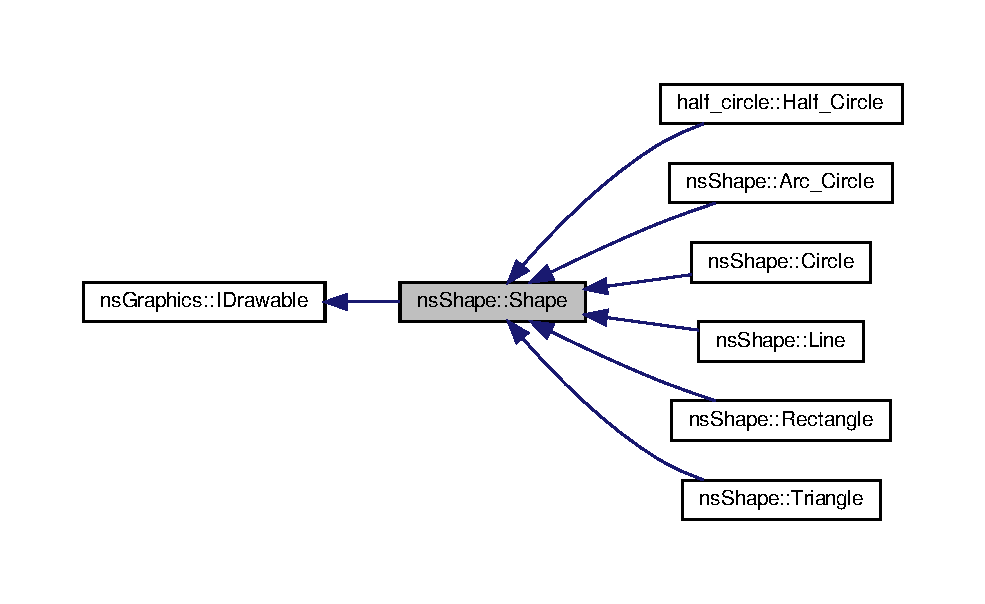
\includegraphics[width=350pt]{classns_shape_1_1_shape__inherit__graph}
\end{center}
\end{figure}


Collaboration diagram for ns\+Shape\+:\+:Shape\+:
\nopagebreak
\begin{figure}[H]
\begin{center}
\leavevmode
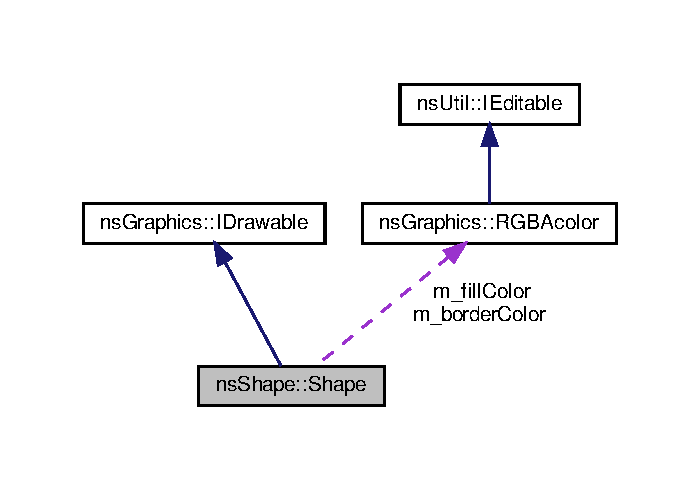
\includegraphics[width=336pt]{classns_shape_1_1_shape__coll__graph}
\end{center}
\end{figure}
\subsection*{Public Member Functions}
\begin{DoxyCompactItemize}
\item 
\hyperlink{classns_shape_1_1_shape_a879f450649c23c83dee576234703951d}{Shape} (const \hyperlink{classns_graphics_1_1_r_g_b_acolor}{ns\+Graphics\+::\+R\+G\+B\+Acolor} \&fill\+Color, const \hyperlink{classns_graphics_1_1_r_g_b_acolor}{ns\+Graphics\+::\+R\+G\+B\+Acolor} \&border\+Color)
\begin{DoxyCompactList}\small\item\em Constructeur pour la classe \hyperlink{classns_shape_1_1_shape}{Shape}. \end{DoxyCompactList}\item 
virtual \hyperlink{classns_shape_1_1_shape_aaa22752af0d45c4e219e3870baf899d4}{$\sim$\+Shape} ()=default
\begin{DoxyCompactList}\small\item\em Destructeur virtuel pour la classe \hyperlink{classns_shape_1_1_shape}{Shape}. \end{DoxyCompactList}\item 
const \hyperlink{classns_graphics_1_1_r_g_b_acolor}{ns\+Graphics\+::\+R\+G\+B\+Acolor} \& \hyperlink{classns_shape_1_1_shape_a8efbd1ac47497b188edeb019557ef754}{get\+Fill\+Color} () const
\begin{DoxyCompactList}\small\item\em Retourne la couleur de remplissage. \end{DoxyCompactList}\item 
void \hyperlink{classns_shape_1_1_shape_aa0e9b22c076b83c4d5014b0213e5ce07}{set\+Fill\+Color} (const \hyperlink{classns_graphics_1_1_r_g_b_acolor}{ns\+Graphics\+::\+R\+G\+B\+Acolor} \&fill\+Color)
\begin{DoxyCompactList}\small\item\em Règle la couleur de remplissage. \end{DoxyCompactList}\item 
const \hyperlink{classns_graphics_1_1_r_g_b_acolor}{ns\+Graphics\+::\+R\+G\+B\+Acolor} \& \hyperlink{classns_shape_1_1_shape_aca75f4b06e8e5b04d0271d191210299d}{get\+Border\+Color} () const
\begin{DoxyCompactList}\small\item\em Retourne la couleur de bord. \end{DoxyCompactList}\item 
void \hyperlink{classns_shape_1_1_shape_a48821100aa1856f188bdba257505adc3}{set\+Border\+Color} (const \hyperlink{classns_graphics_1_1_r_g_b_acolor}{ns\+Graphics\+::\+R\+G\+B\+Acolor} \&border\+Color)
\begin{DoxyCompactList}\small\item\em Règle la couleur de bord. \end{DoxyCompactList}\end{DoxyCompactItemize}
\subsection*{Protected Attributes}
\begin{DoxyCompactItemize}
\item 
\hyperlink{classns_graphics_1_1_r_g_b_acolor}{ns\+Graphics\+::\+R\+G\+B\+Acolor} \hyperlink{classns_shape_1_1_shape_a68841e117adddc95734dcbaa62f68832}{m\+\_\+fill\+Color}
\begin{DoxyCompactList}\small\item\em m\+\_\+fill\+Color \+: Couleur de remplissage \end{DoxyCompactList}\item 
\hyperlink{classns_graphics_1_1_r_g_b_acolor}{ns\+Graphics\+::\+R\+G\+B\+Acolor} \hyperlink{classns_shape_1_1_shape_a0444014e3ee0fa1e6ba5295e530a4f82}{m\+\_\+border\+Color}
\begin{DoxyCompactList}\small\item\em m\+\_\+border\+Color \+: Couleur de bord \end{DoxyCompactList}\end{DoxyCompactItemize}


\subsection{Detailed Description}
Classe de base pour une forme. 

Definition at line 29 of file shape.\+h.



\subsection{Constructor \& Destructor Documentation}
\mbox{\Hypertarget{classns_shape_1_1_shape_a879f450649c23c83dee576234703951d}\label{classns_shape_1_1_shape_a879f450649c23c83dee576234703951d}} 
\index{ns\+Shape\+::\+Shape@{ns\+Shape\+::\+Shape}!Shape@{Shape}}
\index{Shape@{Shape}!ns\+Shape\+::\+Shape@{ns\+Shape\+::\+Shape}}
\subsubsection{\texorpdfstring{Shape()}{Shape()}}
{\footnotesize\ttfamily ns\+Shape\+::\+Shape\+::\+Shape (\begin{DoxyParamCaption}\item[{const \hyperlink{classns_graphics_1_1_r_g_b_acolor}{ns\+Graphics\+::\+R\+G\+B\+Acolor} \&}]{fill\+Color,  }\item[{const \hyperlink{classns_graphics_1_1_r_g_b_acolor}{ns\+Graphics\+::\+R\+G\+B\+Acolor} \&}]{border\+Color }\end{DoxyParamCaption})}



Constructeur pour la classe \hyperlink{classns_shape_1_1_shape}{Shape}. 


\begin{DoxyParams}[1]{Parameters}
\mbox{\tt in}  & {\em fill\+Color} & \+: Couleur de remplissage de la forme \\
\hline
\mbox{\tt in}  & {\em border\+Color} & \+: Couleur de bord de la forme \\
\hline
\end{DoxyParams}
\mbox{\Hypertarget{classns_shape_1_1_shape_aaa22752af0d45c4e219e3870baf899d4}\label{classns_shape_1_1_shape_aaa22752af0d45c4e219e3870baf899d4}} 
\index{ns\+Shape\+::\+Shape@{ns\+Shape\+::\+Shape}!````~Shape@{$\sim$\+Shape}}
\index{````~Shape@{$\sim$\+Shape}!ns\+Shape\+::\+Shape@{ns\+Shape\+::\+Shape}}
\subsubsection{\texorpdfstring{$\sim$\+Shape()}{~Shape()}}
{\footnotesize\ttfamily ns\+Shape\+::\+Shape\+::$\sim$\+Shape (\begin{DoxyParamCaption}{ }\end{DoxyParamCaption})\hspace{0.3cm}{\ttfamily [virtual]}, {\ttfamily [default]}}



Destructeur virtuel pour la classe \hyperlink{classns_shape_1_1_shape}{Shape}. 



\subsection{Member Function Documentation}
\mbox{\Hypertarget{classns_shape_1_1_shape_aca75f4b06e8e5b04d0271d191210299d}\label{classns_shape_1_1_shape_aca75f4b06e8e5b04d0271d191210299d}} 
\index{ns\+Shape\+::\+Shape@{ns\+Shape\+::\+Shape}!get\+Border\+Color@{get\+Border\+Color}}
\index{get\+Border\+Color@{get\+Border\+Color}!ns\+Shape\+::\+Shape@{ns\+Shape\+::\+Shape}}
\subsubsection{\texorpdfstring{get\+Border\+Color()}{getBorderColor()}}
{\footnotesize\ttfamily const \hyperlink{classns_graphics_1_1_r_g_b_acolor}{ns\+Graphics\+::\+R\+G\+B\+Acolor} \& ns\+Shape\+::\+Shape\+::get\+Border\+Color (\begin{DoxyParamCaption}{ }\end{DoxyParamCaption}) const}



Retourne la couleur de bord. 

\mbox{\Hypertarget{classns_shape_1_1_shape_a8efbd1ac47497b188edeb019557ef754}\label{classns_shape_1_1_shape_a8efbd1ac47497b188edeb019557ef754}} 
\index{ns\+Shape\+::\+Shape@{ns\+Shape\+::\+Shape}!get\+Fill\+Color@{get\+Fill\+Color}}
\index{get\+Fill\+Color@{get\+Fill\+Color}!ns\+Shape\+::\+Shape@{ns\+Shape\+::\+Shape}}
\subsubsection{\texorpdfstring{get\+Fill\+Color()}{getFillColor()}}
{\footnotesize\ttfamily const \hyperlink{classns_graphics_1_1_r_g_b_acolor}{ns\+Graphics\+::\+R\+G\+B\+Acolor} \& ns\+Shape\+::\+Shape\+::get\+Fill\+Color (\begin{DoxyParamCaption}{ }\end{DoxyParamCaption}) const}



Retourne la couleur de remplissage. 

\mbox{\Hypertarget{classns_shape_1_1_shape_a48821100aa1856f188bdba257505adc3}\label{classns_shape_1_1_shape_a48821100aa1856f188bdba257505adc3}} 
\index{ns\+Shape\+::\+Shape@{ns\+Shape\+::\+Shape}!set\+Border\+Color@{set\+Border\+Color}}
\index{set\+Border\+Color@{set\+Border\+Color}!ns\+Shape\+::\+Shape@{ns\+Shape\+::\+Shape}}
\subsubsection{\texorpdfstring{set\+Border\+Color()}{setBorderColor()}}
{\footnotesize\ttfamily void ns\+Shape\+::\+Shape\+::set\+Border\+Color (\begin{DoxyParamCaption}\item[{const \hyperlink{classns_graphics_1_1_r_g_b_acolor}{ns\+Graphics\+::\+R\+G\+B\+Acolor} \&}]{border\+Color }\end{DoxyParamCaption})}



Règle la couleur de bord. 

\mbox{\Hypertarget{classns_shape_1_1_shape_aa0e9b22c076b83c4d5014b0213e5ce07}\label{classns_shape_1_1_shape_aa0e9b22c076b83c4d5014b0213e5ce07}} 
\index{ns\+Shape\+::\+Shape@{ns\+Shape\+::\+Shape}!set\+Fill\+Color@{set\+Fill\+Color}}
\index{set\+Fill\+Color@{set\+Fill\+Color}!ns\+Shape\+::\+Shape@{ns\+Shape\+::\+Shape}}
\subsubsection{\texorpdfstring{set\+Fill\+Color()}{setFillColor()}}
{\footnotesize\ttfamily cvoid ns\+Shape\+::\+Shape\+::set\+Fill\+Color (\begin{DoxyParamCaption}\item[{const \hyperlink{classns_graphics_1_1_r_g_b_acolor}{ns\+Graphics\+::\+R\+G\+B\+Acolor} \&}]{fill\+Color }\end{DoxyParamCaption})}



Règle la couleur de remplissage. 



\subsection{Member Data Documentation}
\mbox{\Hypertarget{classns_shape_1_1_shape_a0444014e3ee0fa1e6ba5295e530a4f82}\label{classns_shape_1_1_shape_a0444014e3ee0fa1e6ba5295e530a4f82}} 
\index{ns\+Shape\+::\+Shape@{ns\+Shape\+::\+Shape}!m\+\_\+border\+Color@{m\+\_\+border\+Color}}
\index{m\+\_\+border\+Color@{m\+\_\+border\+Color}!ns\+Shape\+::\+Shape@{ns\+Shape\+::\+Shape}}
\subsubsection{\texorpdfstring{m\+\_\+border\+Color}{m\_borderColor}}
{\footnotesize\ttfamily \hyperlink{classns_graphics_1_1_r_g_b_acolor}{ns\+Graphics\+::\+R\+G\+B\+Acolor} ns\+Shape\+::\+Shape\+::m\+\_\+border\+Color\hspace{0.3cm}{\ttfamily [protected]}}



m\+\_\+border\+Color \+: Couleur de bord 



Definition at line 80 of file shape.\+h.

\mbox{\Hypertarget{classns_shape_1_1_shape_a68841e117adddc95734dcbaa62f68832}\label{classns_shape_1_1_shape_a68841e117adddc95734dcbaa62f68832}} 
\index{ns\+Shape\+::\+Shape@{ns\+Shape\+::\+Shape}!m\+\_\+fill\+Color@{m\+\_\+fill\+Color}}
\index{m\+\_\+fill\+Color@{m\+\_\+fill\+Color}!ns\+Shape\+::\+Shape@{ns\+Shape\+::\+Shape}}
\subsubsection{\texorpdfstring{m\+\_\+fill\+Color}{m\_fillColor}}
{\footnotesize\ttfamily \hyperlink{classns_graphics_1_1_r_g_b_acolor}{ns\+Graphics\+::\+R\+G\+B\+Acolor} ns\+Shape\+::\+Shape\+::m\+\_\+fill\+Color\hspace{0.3cm}{\ttfamily [protected]}}



m\+\_\+fill\+Color \+: Couleur de remplissage 



Definition at line 75 of file shape.\+h.



The documentation for this class was generated from the following file\+:\begin{DoxyCompactItemize}
\item 
libs/mingl/shape/\hyperlink{shape_8h}{shape.\+h}\end{DoxyCompactItemize}

\hypertarget{structshield_1_1_shield}{}\section{shield\+:\+:Shield Struct Reference}
\label{structshield_1_1_shield}\index{shield\+::\+Shield@{shield\+::\+Shield}}


Structure des bouclier.  




{\ttfamily \#include $<$shield.\+h$>$}



Collaboration diagram for shield\+:\+:Shield\+:
\nopagebreak
\begin{figure}[H]
\begin{center}
\leavevmode
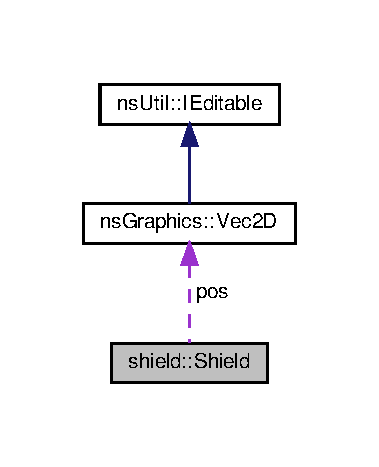
\includegraphics[width=182pt]{structshield_1_1_shield__coll__graph}
\end{center}
\end{figure}
\subsection*{Public Member Functions}
\begin{DoxyCompactItemize}
\item 
\hyperlink{structshield_1_1_shield_addde44a42ca29e8d6474dbd52449aa40}{Shield} (const \hyperlink{classns_graphics_1_1_vec2_d}{ns\+Graphics\+::\+Vec2D} \&ent\+Pos)
\begin{DoxyCompactList}\small\item\em Fonction constructeur du bouclier. \end{DoxyCompactList}\item 
void \hyperlink{structshield_1_1_shield_a768986dee4a088af222f1b987a91d62d}{show} (\hyperlink{class_min_g_l}{Min\+GL} \&window)
\begin{DoxyCompactList}\small\item\em Permet d\textquotesingle{}afficher graphiquement le bouclier. \end{DoxyCompactList}\end{DoxyCompactItemize}
\subsection*{Public Attributes}
\begin{DoxyCompactItemize}
\item 
unsigned \hyperlink{structshield_1_1_shield_aec13726342753b52ec6954b5ced3497d}{life}
\item 
\hyperlink{classns_graphics_1_1_vec2_d}{ns\+Graphics\+::\+Vec2D} \hyperlink{structshield_1_1_shield_aee8c1d30a8e23c2097048a04efe9d01b}{pos}
\end{DoxyCompactItemize}


\subsection{Detailed Description}
Structure des bouclier. 

Definition at line 21 of file shield.\+h.



\subsection{Constructor \& Destructor Documentation}
\mbox{\Hypertarget{structshield_1_1_shield_addde44a42ca29e8d6474dbd52449aa40}\label{structshield_1_1_shield_addde44a42ca29e8d6474dbd52449aa40}} 
\index{shield\+::\+Shield@{shield\+::\+Shield}!Shield@{Shield}}
\index{Shield@{Shield}!shield\+::\+Shield@{shield\+::\+Shield}}
\subsubsection{\texorpdfstring{Shield()}{Shield()}}
{\footnotesize\ttfamily shield\+::\+Shield\+::\+Shield (\begin{DoxyParamCaption}\item[{const \hyperlink{classns_graphics_1_1_vec2_d}{ns\+Graphics\+::\+Vec2D} \&}]{ent\+Pos }\end{DoxyParamCaption})}



Fonction constructeur du bouclier. 


\begin{DoxyParams}[1]{Parameters}
\mbox{\tt in}  & {\em ent\+Pos} & \+: position du bouclier \\
\hline
\end{DoxyParams}


Definition at line 7 of file shield.\+cpp.



\subsection{Member Function Documentation}
\mbox{\Hypertarget{structshield_1_1_shield_a768986dee4a088af222f1b987a91d62d}\label{structshield_1_1_shield_a768986dee4a088af222f1b987a91d62d}} 
\index{shield\+::\+Shield@{shield\+::\+Shield}!show@{show}}
\index{show@{show}!shield\+::\+Shield@{shield\+::\+Shield}}
\subsubsection{\texorpdfstring{show()}{show()}}
{\footnotesize\ttfamily void shield\+::\+Shield\+::show (\begin{DoxyParamCaption}\item[{\hyperlink{class_min_g_l}{Min\+GL} \&}]{window }\end{DoxyParamCaption})}



Permet d\textquotesingle{}afficher graphiquement le bouclier. 


\begin{DoxyParams}[1]{Parameters}
\mbox{\tt in,out}  & {\em window} & \+: fenêtre de jeu \\
\hline
\end{DoxyParams}


Definition at line 12 of file shield.\+cpp.



\subsection{Member Data Documentation}
\mbox{\Hypertarget{structshield_1_1_shield_aec13726342753b52ec6954b5ced3497d}\label{structshield_1_1_shield_aec13726342753b52ec6954b5ced3497d}} 
\index{shield\+::\+Shield@{shield\+::\+Shield}!life@{life}}
\index{life@{life}!shield\+::\+Shield@{shield\+::\+Shield}}
\subsubsection{\texorpdfstring{life}{life}}
{\footnotesize\ttfamily unsigned shield\+::\+Shield\+::life}



Definition at line 23 of file shield.\+h.

\mbox{\Hypertarget{structshield_1_1_shield_aee8c1d30a8e23c2097048a04efe9d01b}\label{structshield_1_1_shield_aee8c1d30a8e23c2097048a04efe9d01b}} 
\index{shield\+::\+Shield@{shield\+::\+Shield}!pos@{pos}}
\index{pos@{pos}!shield\+::\+Shield@{shield\+::\+Shield}}
\subsubsection{\texorpdfstring{pos}{pos}}
{\footnotesize\ttfamily \hyperlink{classns_graphics_1_1_vec2_d}{ns\+Graphics\+::\+Vec2D} shield\+::\+Shield\+::pos}



Definition at line 24 of file shield.\+h.



The documentation for this struct was generated from the following files\+:\begin{DoxyCompactItemize}
\item 
libs/game/entities/\hyperlink{shield_8h}{shield.\+h}\item 
src/entities/\hyperlink{shield_8cpp}{shield.\+cpp}\end{DoxyCompactItemize}

\hypertarget{classns_gui_1_1_sprite}{}\section{ns\+Gui\+:\+:Sprite Class Reference}
\label{classns_gui_1_1_sprite}\index{ns\+Gui\+::\+Sprite@{ns\+Gui\+::\+Sprite}}


Permet de charger une image depuis un format créé pour l\textquotesingle{}occasion, le .si2.  




{\ttfamily \#include $<$sprite.\+h$>$}



Inheritance diagram for ns\+Gui\+:\+:Sprite\+:
\nopagebreak
\begin{figure}[H]
\begin{center}
\leavevmode
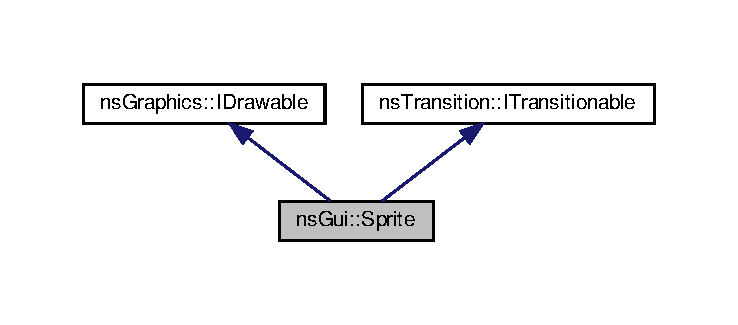
\includegraphics[width=350pt]{classns_gui_1_1_sprite__inherit__graph}
\end{center}
\end{figure}


Collaboration diagram for ns\+Gui\+:\+:Sprite\+:
\nopagebreak
\begin{figure}[H]
\begin{center}
\leavevmode
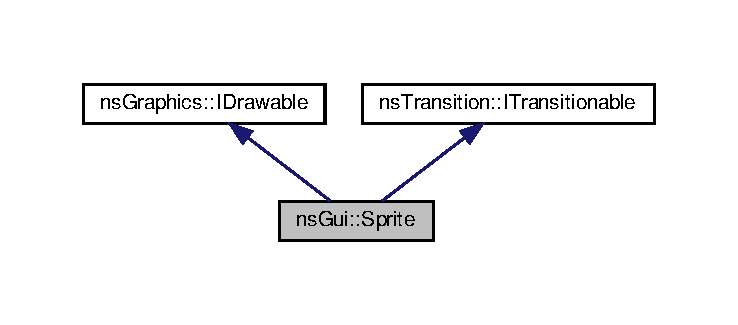
\includegraphics[width=350pt]{classns_gui_1_1_sprite__coll__graph}
\end{center}
\end{figure}
\subsection*{Public Types}
\begin{DoxyCompactItemize}
\item 
enum \hyperlink{classns_gui_1_1_sprite_a09069244e6b3e580f8511496c7ae1b78}{Transition\+Ids} \{ \hyperlink{classns_gui_1_1_sprite_a09069244e6b3e580f8511496c7ae1b78a90092e9cd093f4ef21dab0a68fbe6c54}{T\+R\+A\+N\+S\+I\+T\+I\+O\+N\+\_\+\+P\+O\+S\+I\+T\+I\+ON}
 \}\begin{DoxyCompactList}\small\item\em Transition\+Ids \+: Liste de toutes les transitions que cet élément peut exécuter. \end{DoxyCompactList}
\end{DoxyCompactItemize}
\subsection*{Public Member Functions}
\begin{DoxyCompactItemize}
\item 
\hyperlink{classns_gui_1_1_sprite_a35558b08dfeb3e3a20be52da28e33c4c}{Sprite} (const std\+::string \&filename, const \hyperlink{classns_graphics_1_1_vec2_d}{ns\+Graphics\+::\+Vec2D} \&position=\hyperlink{classns_graphics_1_1_vec2_d}{ns\+Graphics\+::\+Vec2D}())
\begin{DoxyCompactList}\small\item\em Constructeur pour la classe \hyperlink{classns_gui_1_1_sprite}{Sprite}, charge les données depuis un fichier. \end{DoxyCompactList}\item 
\hyperlink{classns_gui_1_1_sprite_abee8e5a2740555d46f19af3d4b489453}{Sprite} (const std\+::vector$<$ \hyperlink{classns_graphics_1_1_r_g_b_acolor}{ns\+Graphics\+::\+R\+G\+B\+Acolor} $>$ \&pixel\+Data, const uint32\+\_\+t \&\hyperlink{sprite_8h_a410460a0a75462ae38c5c9daf5fb06ed}{row\+Size}, const \hyperlink{classns_graphics_1_1_vec2_d}{ns\+Graphics\+::\+Vec2D} \&position=\hyperlink{classns_graphics_1_1_vec2_d}{ns\+Graphics\+::\+Vec2D}())
\begin{DoxyCompactList}\small\item\em Constructeur pour la classe \hyperlink{classns_gui_1_1_sprite}{Sprite}, copie les données depuis un vecteur de pixels. \end{DoxyCompactList}\item 
virtual void \hyperlink{classns_gui_1_1_sprite_a15157c69a1d792080d2b41519659418c}{draw} (\hyperlink{class_min_g_l}{Min\+GL} \&window) const override
\begin{DoxyCompactList}\small\item\em Fonction pour afficher l\textquotesingle{}objet. \end{DoxyCompactList}\item 
virtual void \hyperlink{classns_gui_1_1_sprite_a19cd382e454660efd8a20ee30ba3cc8c}{get\+Values} (const int \&id, std\+::vector$<$ float $>$ \&values) override
\begin{DoxyCompactList}\small\item\em Récupère des valeurs dans un vecteur de float pour l\textquotesingle{}ID spécifié \end{DoxyCompactList}\item 
virtual void \hyperlink{classns_gui_1_1_sprite_a4259e3283228980136e06d2a41a75d31}{set\+Values} (const int \&id, const std\+::vector$<$ float $>$ \&values) override
\begin{DoxyCompactList}\small\item\em Définit les nouvelles valeurs pour l\textquotesingle{}ID spécifié \end{DoxyCompactList}\item 
const uint32\+\_\+t \& \hyperlink{classns_gui_1_1_sprite_adbe04bd427b6658e0181ce167db83d05}{get\+Row\+Size} () const
\begin{DoxyCompactList}\small\item\em Récupère le nombre de pixels par ligne. \end{DoxyCompactList}\item 
const std\+::vector$<$ \hyperlink{classns_graphics_1_1_r_g_b_acolor}{ns\+Graphics\+::\+R\+G\+B\+Acolor} $>$ \& \hyperlink{classns_gui_1_1_sprite_ad8644780a7a7dcbcd5f2e4e7a461b685}{get\+Pixel\+Data} () const
\begin{DoxyCompactList}\small\item\em Récupère le vecteur contenant les pixels de l\textquotesingle{}image. \end{DoxyCompactList}\item 
const \hyperlink{classns_graphics_1_1_vec2_d}{ns\+Graphics\+::\+Vec2D} \& \hyperlink{classns_gui_1_1_sprite_a1d6ad6681627aae6c4680fc936da8eb2}{get\+Position} () const
\begin{DoxyCompactList}\small\item\em Récupère la position du sprite. \end{DoxyCompactList}\item 
void \hyperlink{classns_gui_1_1_sprite_a4c695910c46504d1e8d47b838394a48e}{set\+Position} (const \hyperlink{classns_graphics_1_1_vec2_d}{ns\+Graphics\+::\+Vec2D} \&position)
\begin{DoxyCompactList}\small\item\em Définit la nouvelle position du sprite. \end{DoxyCompactList}\item 
\hyperlink{classns_graphics_1_1_vec2_d}{ns\+Graphics\+::\+Vec2D} \hyperlink{classns_gui_1_1_sprite_a26b502e88906860373c278495794998c}{compute\+Size} () const
\begin{DoxyCompactList}\small\item\em Calcule la taille du sprite. \end{DoxyCompactList}\end{DoxyCompactItemize}


\subsection{Detailed Description}
Permet de charger une image depuis un format créé pour l\textquotesingle{}occasion, le .si2. 

Definition at line 28 of file sprite.\+h.



\subsection{Member Enumeration Documentation}
\mbox{\Hypertarget{classns_gui_1_1_sprite_a09069244e6b3e580f8511496c7ae1b78}\label{classns_gui_1_1_sprite_a09069244e6b3e580f8511496c7ae1b78}} 
\index{ns\+Gui\+::\+Sprite@{ns\+Gui\+::\+Sprite}!Transition\+Ids@{Transition\+Ids}}
\index{Transition\+Ids@{Transition\+Ids}!ns\+Gui\+::\+Sprite@{ns\+Gui\+::\+Sprite}}
\subsubsection{\texorpdfstring{Transition\+Ids}{TransitionIds}}
{\footnotesize\ttfamily enum \hyperlink{classns_gui_1_1_sprite_a09069244e6b3e580f8511496c7ae1b78}{ns\+Gui\+::\+Sprite\+::\+Transition\+Ids}}



Transition\+Ids \+: Liste de toutes les transitions que cet élément peut exécuter. 

\begin{DoxyEnumFields}{Enumerator}
\raisebox{\heightof{T}}[0pt][0pt]{\index{T\+R\+A\+N\+S\+I\+T\+I\+O\+N\+\_\+\+P\+O\+S\+I\+T\+I\+ON@{T\+R\+A\+N\+S\+I\+T\+I\+O\+N\+\_\+\+P\+O\+S\+I\+T\+I\+ON}!ns\+Gui\+::\+Sprite@{ns\+Gui\+::\+Sprite}}\index{ns\+Gui\+::\+Sprite@{ns\+Gui\+::\+Sprite}!T\+R\+A\+N\+S\+I\+T\+I\+O\+N\+\_\+\+P\+O\+S\+I\+T\+I\+ON@{T\+R\+A\+N\+S\+I\+T\+I\+O\+N\+\_\+\+P\+O\+S\+I\+T\+I\+ON}}}\mbox{\Hypertarget{classns_gui_1_1_sprite_a09069244e6b3e580f8511496c7ae1b78a90092e9cd093f4ef21dab0a68fbe6c54}\label{classns_gui_1_1_sprite_a09069244e6b3e580f8511496c7ae1b78a90092e9cd093f4ef21dab0a68fbe6c54}} 
T\+R\+A\+N\+S\+I\+T\+I\+O\+N\+\_\+\+P\+O\+S\+I\+T\+I\+ON&Transition pour la position \\
\hline

\end{DoxyEnumFields}


Definition at line 34 of file sprite.\+h.



\subsection{Constructor \& Destructor Documentation}
\mbox{\Hypertarget{classns_gui_1_1_sprite_a35558b08dfeb3e3a20be52da28e33c4c}\label{classns_gui_1_1_sprite_a35558b08dfeb3e3a20be52da28e33c4c}} 
\index{ns\+Gui\+::\+Sprite@{ns\+Gui\+::\+Sprite}!Sprite@{Sprite}}
\index{Sprite@{Sprite}!ns\+Gui\+::\+Sprite@{ns\+Gui\+::\+Sprite}}
\subsubsection{\texorpdfstring{Sprite()}{Sprite()}\hspace{0.1cm}{\footnotesize\ttfamily [1/2]}}
{\footnotesize\ttfamily ns\+Gui\+::\+Sprite\+::\+Sprite (\begin{DoxyParamCaption}\item[{const std\+::string \&}]{filename,  }\item[{const \hyperlink{classns_graphics_1_1_vec2_d}{ns\+Graphics\+::\+Vec2D} \&}]{position = {\ttfamily \hyperlink{classns_graphics_1_1_vec2_d}{ns\+Graphics\+::\+Vec2D}()} }\end{DoxyParamCaption})}



Constructeur pour la classe \hyperlink{classns_gui_1_1_sprite}{Sprite}, charge les données depuis un fichier. 


\begin{DoxyParams}[1]{Parameters}
\mbox{\tt in}  & {\em filename} & \+: Chemin d\textquotesingle{}accès vers le fichier image \\
\hline
\mbox{\tt in}  & {\em position} & \+: Position du sprite \\
\hline
\end{DoxyParams}
\mbox{\Hypertarget{classns_gui_1_1_sprite_abee8e5a2740555d46f19af3d4b489453}\label{classns_gui_1_1_sprite_abee8e5a2740555d46f19af3d4b489453}} 
\index{ns\+Gui\+::\+Sprite@{ns\+Gui\+::\+Sprite}!Sprite@{Sprite}}
\index{Sprite@{Sprite}!ns\+Gui\+::\+Sprite@{ns\+Gui\+::\+Sprite}}
\subsubsection{\texorpdfstring{Sprite()}{Sprite()}\hspace{0.1cm}{\footnotesize\ttfamily [2/2]}}
{\footnotesize\ttfamily ns\+Gui\+::\+Sprite\+::\+Sprite (\begin{DoxyParamCaption}\item[{const std\+::vector$<$ \hyperlink{classns_graphics_1_1_r_g_b_acolor}{ns\+Graphics\+::\+R\+G\+B\+Acolor} $>$ \&}]{pixel\+Data,  }\item[{const uint32\+\_\+t \&}]{row\+Size,  }\item[{const \hyperlink{classns_graphics_1_1_vec2_d}{ns\+Graphics\+::\+Vec2D} \&}]{position = {\ttfamily \hyperlink{classns_graphics_1_1_vec2_d}{ns\+Graphics\+::\+Vec2D}()} }\end{DoxyParamCaption})}



Constructeur pour la classe \hyperlink{classns_gui_1_1_sprite}{Sprite}, copie les données depuis un vecteur de pixels. 


\begin{DoxyParams}[1]{Parameters}
\mbox{\tt in}  & {\em pixel\+Data} & \+: Vecteur contenant des données sur les pixels \\
\hline
\mbox{\tt in}  & {\em row\+Size} & \+: Nombre de pixels par ligne \\
\hline
\mbox{\tt in}  & {\em position} & \+: Position du sprite \\
\hline
\end{DoxyParams}


\subsection{Member Function Documentation}
\mbox{\Hypertarget{classns_gui_1_1_sprite_a26b502e88906860373c278495794998c}\label{classns_gui_1_1_sprite_a26b502e88906860373c278495794998c}} 
\index{ns\+Gui\+::\+Sprite@{ns\+Gui\+::\+Sprite}!compute\+Size@{compute\+Size}}
\index{compute\+Size@{compute\+Size}!ns\+Gui\+::\+Sprite@{ns\+Gui\+::\+Sprite}}
\subsubsection{\texorpdfstring{compute\+Size()}{computeSize()}}
{\footnotesize\ttfamily Vec2D ns\+Gui\+::\+Sprite\+::compute\+Size (\begin{DoxyParamCaption}{ }\end{DoxyParamCaption}) const}



Calcule la taille du sprite. 

\begin{DoxyReturn}{Returns}
La taille calculée 
\end{DoxyReturn}
\mbox{\Hypertarget{classns_gui_1_1_sprite_a15157c69a1d792080d2b41519659418c}\label{classns_gui_1_1_sprite_a15157c69a1d792080d2b41519659418c}} 
\index{ns\+Gui\+::\+Sprite@{ns\+Gui\+::\+Sprite}!draw@{draw}}
\index{draw@{draw}!ns\+Gui\+::\+Sprite@{ns\+Gui\+::\+Sprite}}
\subsubsection{\texorpdfstring{draw()}{draw()}}
{\footnotesize\ttfamily virtual void ns\+Gui\+::\+Sprite\+::draw (\begin{DoxyParamCaption}\item[{\hyperlink{class_min_g_l}{Min\+GL} \&}]{window }\end{DoxyParamCaption}) const\hspace{0.3cm}{\ttfamily [override]}, {\ttfamily [virtual]}}



Fonction pour afficher l\textquotesingle{}objet. 



Implements \hyperlink{classns_graphics_1_1_i_drawable_abed8a61e1d507d31e76f0891f3bf9c51}{ns\+Graphics\+::\+I\+Drawable}.

\mbox{\Hypertarget{classns_gui_1_1_sprite_ad8644780a7a7dcbcd5f2e4e7a461b685}\label{classns_gui_1_1_sprite_ad8644780a7a7dcbcd5f2e4e7a461b685}} 
\index{ns\+Gui\+::\+Sprite@{ns\+Gui\+::\+Sprite}!get\+Pixel\+Data@{get\+Pixel\+Data}}
\index{get\+Pixel\+Data@{get\+Pixel\+Data}!ns\+Gui\+::\+Sprite@{ns\+Gui\+::\+Sprite}}
\subsubsection{\texorpdfstring{get\+Pixel\+Data()}{getPixelData()}}
{\footnotesize\ttfamily const std\+::vector$<$ \hyperlink{classns_graphics_1_1_r_g_b_acolor}{ns\+Graphics\+::\+R\+G\+B\+Acolor} $>$ \& ns\+Gui\+::\+Sprite\+::get\+Pixel\+Data (\begin{DoxyParamCaption}{ }\end{DoxyParamCaption}) const}



Récupère le vecteur contenant les pixels de l\textquotesingle{}image. 

\begin{DoxyReturn}{Returns}
Une référence constante vers m\+\_\+pixel\+Data 
\end{DoxyReturn}
\mbox{\Hypertarget{classns_gui_1_1_sprite_a1d6ad6681627aae6c4680fc936da8eb2}\label{classns_gui_1_1_sprite_a1d6ad6681627aae6c4680fc936da8eb2}} 
\index{ns\+Gui\+::\+Sprite@{ns\+Gui\+::\+Sprite}!get\+Position@{get\+Position}}
\index{get\+Position@{get\+Position}!ns\+Gui\+::\+Sprite@{ns\+Gui\+::\+Sprite}}
\subsubsection{\texorpdfstring{get\+Position()}{getPosition()}}
{\footnotesize\ttfamily const \hyperlink{classns_graphics_1_1_vec2_d}{ns\+Graphics\+::\+Vec2D} \& ns\+Gui\+::\+Sprite\+::get\+Position (\begin{DoxyParamCaption}{ }\end{DoxyParamCaption}) const}



Récupère la position du sprite. 

\begin{DoxyReturn}{Returns}
Une référence const vers m\+\_\+position 
\end{DoxyReturn}
\mbox{\Hypertarget{classns_gui_1_1_sprite_adbe04bd427b6658e0181ce167db83d05}\label{classns_gui_1_1_sprite_adbe04bd427b6658e0181ce167db83d05}} 
\index{ns\+Gui\+::\+Sprite@{ns\+Gui\+::\+Sprite}!get\+Row\+Size@{get\+Row\+Size}}
\index{get\+Row\+Size@{get\+Row\+Size}!ns\+Gui\+::\+Sprite@{ns\+Gui\+::\+Sprite}}
\subsubsection{\texorpdfstring{get\+Row\+Size()}{getRowSize()}}
{\footnotesize\ttfamily const uint32\+\_\+t \& ns\+Gui\+::\+Sprite\+::get\+Row\+Size (\begin{DoxyParamCaption}{ }\end{DoxyParamCaption}) const}



Récupère le nombre de pixels par ligne. 

\begin{DoxyReturn}{Returns}
Une référence constante vers m\+\_\+row\+Size 
\end{DoxyReturn}
\mbox{\Hypertarget{classns_gui_1_1_sprite_a19cd382e454660efd8a20ee30ba3cc8c}\label{classns_gui_1_1_sprite_a19cd382e454660efd8a20ee30ba3cc8c}} 
\index{ns\+Gui\+::\+Sprite@{ns\+Gui\+::\+Sprite}!get\+Values@{get\+Values}}
\index{get\+Values@{get\+Values}!ns\+Gui\+::\+Sprite@{ns\+Gui\+::\+Sprite}}
\subsubsection{\texorpdfstring{get\+Values()}{getValues()}}
{\footnotesize\ttfamily virtual void ns\+Gui\+::\+Sprite\+::get\+Values (\begin{DoxyParamCaption}\item[{const int \&}]{id,  }\item[{std\+::vector$<$ float $>$ \&}]{values }\end{DoxyParamCaption})\hspace{0.3cm}{\ttfamily [override]}, {\ttfamily [virtual]}}



Récupère des valeurs dans un vecteur de float pour l\textquotesingle{}ID spécifié 


\begin{DoxyParams}[1]{Parameters}
\mbox{\tt in}  & {\em id} & ID des valeurs a récupérer \\
\hline
\mbox{\tt in,out}  & {\em values} & Vecteur de valeurs a peupler \\
\hline
\end{DoxyParams}


Implements \hyperlink{classns_transition_1_1_i_transitionable_a5871a16fd47c1e5c8bacdd5da8597ed9}{ns\+Transition\+::\+I\+Transitionable}.

\mbox{\Hypertarget{classns_gui_1_1_sprite_a4c695910c46504d1e8d47b838394a48e}\label{classns_gui_1_1_sprite_a4c695910c46504d1e8d47b838394a48e}} 
\index{ns\+Gui\+::\+Sprite@{ns\+Gui\+::\+Sprite}!set\+Position@{set\+Position}}
\index{set\+Position@{set\+Position}!ns\+Gui\+::\+Sprite@{ns\+Gui\+::\+Sprite}}
\subsubsection{\texorpdfstring{set\+Position()}{setPosition()}}
{\footnotesize\ttfamily void ns\+Gui\+::\+Sprite\+::set\+Position (\begin{DoxyParamCaption}\item[{const \hyperlink{classns_graphics_1_1_vec2_d}{ns\+Graphics\+::\+Vec2D} \&}]{position }\end{DoxyParamCaption})}



Définit la nouvelle position du sprite. 


\begin{DoxyParams}[1]{Parameters}
\mbox{\tt in}  & {\em position} & \+: Nouvelle position \\
\hline
\end{DoxyParams}
\mbox{\Hypertarget{classns_gui_1_1_sprite_a4259e3283228980136e06d2a41a75d31}\label{classns_gui_1_1_sprite_a4259e3283228980136e06d2a41a75d31}} 
\index{ns\+Gui\+::\+Sprite@{ns\+Gui\+::\+Sprite}!set\+Values@{set\+Values}}
\index{set\+Values@{set\+Values}!ns\+Gui\+::\+Sprite@{ns\+Gui\+::\+Sprite}}
\subsubsection{\texorpdfstring{set\+Values()}{setValues()}}
{\footnotesize\ttfamily virtual void ns\+Gui\+::\+Sprite\+::set\+Values (\begin{DoxyParamCaption}\item[{const int \&}]{id,  }\item[{const std\+::vector$<$ float $>$ \&}]{values }\end{DoxyParamCaption})\hspace{0.3cm}{\ttfamily [override]}, {\ttfamily [virtual]}}



Définit les nouvelles valeurs pour l\textquotesingle{}ID spécifié 


\begin{DoxyParams}[1]{Parameters}
\mbox{\tt in}  & {\em id} & ID des valeurs a définir \\
\hline
\mbox{\tt in}  & {\em values} & Vecteur des nouvelles valeurs a appliquer \\
\hline
\end{DoxyParams}


Implements \hyperlink{classns_transition_1_1_i_transitionable_ade37d29f7f2ca4890ed0e2e64d033197}{ns\+Transition\+::\+I\+Transitionable}.



The documentation for this class was generated from the following file\+:\begin{DoxyCompactItemize}
\item 
libs/mingl/gui/\hyperlink{sprite_8h}{sprite.\+h}\end{DoxyCompactItemize}

\hypertarget{structstart_game_1_1_start_game}{}\section{start\+Game\+:\+:Start\+Game Struct Reference}
\label{structstart_game_1_1_start_game}\index{start\+Game\+::\+Start\+Game@{start\+Game\+::\+Start\+Game}}


Structure du départ de la partie.  




{\ttfamily \#include $<$start\+Game.\+h$>$}



Collaboration diagram for start\+Game\+:\+:Start\+Game\+:
\nopagebreak
\begin{figure}[H]
\begin{center}
\leavevmode
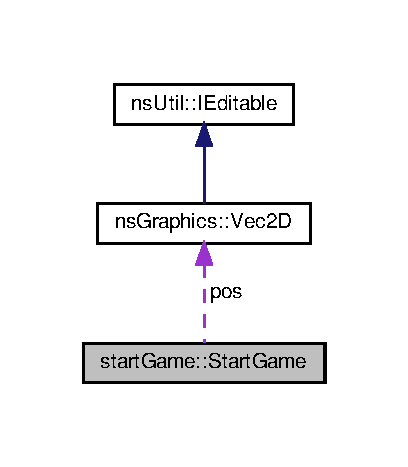
\includegraphics[width=196pt]{structstart_game_1_1_start_game__coll__graph}
\end{center}
\end{figure}
\subsection*{Public Member Functions}
\begin{DoxyCompactItemize}
\item 
\hyperlink{structstart_game_1_1_start_game_a3d839835fe053e4a6357f98a70cdd71e}{Start\+Game} (\hyperlink{class_min_g_l}{Min\+GL} \&window, std\+::vector$<$ unsigned $>$ \&ent\+Size)
\begin{DoxyCompactList}\small\item\em Fonction constructeur de la struct \hyperlink{structstart_game_1_1_start_game}{Start\+Game}. \end{DoxyCompactList}\item 
void \hyperlink{structstart_game_1_1_start_game_a5607dba94483e55cc1855192063e4a58}{show} (\hyperlink{class_min_g_l}{Min\+GL} \&window)
\begin{DoxyCompactList}\small\item\em Fonction qui affiche le départ de la partie. \end{DoxyCompactList}\end{DoxyCompactItemize}
\subsection*{Public Attributes}
\begin{DoxyCompactItemize}
\item 
\hyperlink{classns_graphics_1_1_vec2_d}{ns\+Graphics\+::\+Vec2D} \hyperlink{structstart_game_1_1_start_game_a5eca1a21b445f45875bf9a5116a97a5e}{pos}
\item 
std\+::vector$<$ unsigned $>$ \hyperlink{structstart_game_1_1_start_game_a17f51b9a759839975438d56fcf3f1176}{size}
\end{DoxyCompactItemize}


\subsection{Detailed Description}
Structure du départ de la partie. 

Definition at line 20 of file start\+Game.\+h.



\subsection{Constructor \& Destructor Documentation}
\mbox{\Hypertarget{structstart_game_1_1_start_game_a3d839835fe053e4a6357f98a70cdd71e}\label{structstart_game_1_1_start_game_a3d839835fe053e4a6357f98a70cdd71e}} 
\index{start\+Game\+::\+Start\+Game@{start\+Game\+::\+Start\+Game}!Start\+Game@{Start\+Game}}
\index{Start\+Game@{Start\+Game}!start\+Game\+::\+Start\+Game@{start\+Game\+::\+Start\+Game}}
\subsubsection{\texorpdfstring{Start\+Game()}{StartGame()}}
{\footnotesize\ttfamily start\+Game\+::\+Start\+Game\+::\+Start\+Game (\begin{DoxyParamCaption}\item[{\hyperlink{class_min_g_l}{Min\+GL} \&}]{window,  }\item[{std\+::vector$<$ unsigned $>$ \&}]{ent\+Size }\end{DoxyParamCaption})}



Fonction constructeur de la struct \hyperlink{structstart_game_1_1_start_game}{Start\+Game}. 


\begin{DoxyParams}[1]{Parameters}
\mbox{\tt in}  & {\em window} & \+: fenêtre de jeu \\
\hline
\mbox{\tt in}  & {\em ent\+Size} & \+: taille du start \\
\hline
\end{DoxyParams}


Definition at line 7 of file start\+Game.\+cpp.



\subsection{Member Function Documentation}
\mbox{\Hypertarget{structstart_game_1_1_start_game_a5607dba94483e55cc1855192063e4a58}\label{structstart_game_1_1_start_game_a5607dba94483e55cc1855192063e4a58}} 
\index{start\+Game\+::\+Start\+Game@{start\+Game\+::\+Start\+Game}!show@{show}}
\index{show@{show}!start\+Game\+::\+Start\+Game@{start\+Game\+::\+Start\+Game}}
\subsubsection{\texorpdfstring{show()}{show()}}
{\footnotesize\ttfamily void start\+Game\+::\+Start\+Game\+::show (\begin{DoxyParamCaption}\item[{\hyperlink{class_min_g_l}{Min\+GL} \&}]{window }\end{DoxyParamCaption})}



Fonction qui affiche le départ de la partie. 


\begin{DoxyParams}[1]{Parameters}
\mbox{\tt in,out}  & {\em window} & \+: fenêtre de jeu \\
\hline
\end{DoxyParams}


Definition at line 12 of file start\+Game.\+cpp.



\subsection{Member Data Documentation}
\mbox{\Hypertarget{structstart_game_1_1_start_game_a5eca1a21b445f45875bf9a5116a97a5e}\label{structstart_game_1_1_start_game_a5eca1a21b445f45875bf9a5116a97a5e}} 
\index{start\+Game\+::\+Start\+Game@{start\+Game\+::\+Start\+Game}!pos@{pos}}
\index{pos@{pos}!start\+Game\+::\+Start\+Game@{start\+Game\+::\+Start\+Game}}
\subsubsection{\texorpdfstring{pos}{pos}}
{\footnotesize\ttfamily \hyperlink{classns_graphics_1_1_vec2_d}{ns\+Graphics\+::\+Vec2D} start\+Game\+::\+Start\+Game\+::pos}



Definition at line 23 of file start\+Game.\+h.

\mbox{\Hypertarget{structstart_game_1_1_start_game_a17f51b9a759839975438d56fcf3f1176}\label{structstart_game_1_1_start_game_a17f51b9a759839975438d56fcf3f1176}} 
\index{start\+Game\+::\+Start\+Game@{start\+Game\+::\+Start\+Game}!size@{size}}
\index{size@{size}!start\+Game\+::\+Start\+Game@{start\+Game\+::\+Start\+Game}}
\subsubsection{\texorpdfstring{size}{size}}
{\footnotesize\ttfamily std\+::vector$<$unsigned$>$ start\+Game\+::\+Start\+Game\+::size}



Definition at line 24 of file start\+Game.\+h.



The documentation for this struct was generated from the following files\+:\begin{DoxyCompactItemize}
\item 
libs/game/entities/\hyperlink{start_game_8h}{start\+Game.\+h}\item 
src/entities/\hyperlink{start_game_8cpp}{start\+Game.\+cpp}\end{DoxyCompactItemize}

\hypertarget{classns_gui_1_1_text}{}\section{ns\+Gui\+:\+:Text Class Reference}
\label{classns_gui_1_1_text}\index{ns\+Gui\+::\+Text@{ns\+Gui\+::\+Text}}


Gère l\textquotesingle{}affichage d\textquotesingle{}un texte.  




{\ttfamily \#include $<$text.\+h$>$}



Inheritance diagram for ns\+Gui\+:\+:Text\+:
\nopagebreak
\begin{figure}[H]
\begin{center}
\leavevmode
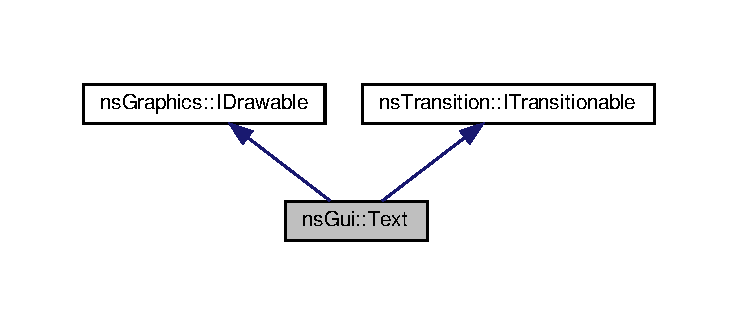
\includegraphics[width=350pt]{classns_gui_1_1_text__inherit__graph}
\end{center}
\end{figure}


Collaboration diagram for ns\+Gui\+:\+:Text\+:
\nopagebreak
\begin{figure}[H]
\begin{center}
\leavevmode
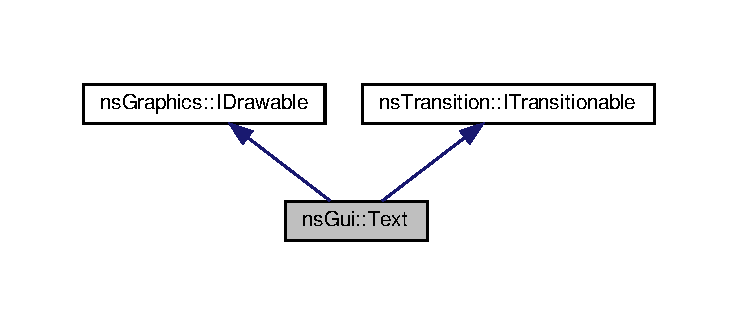
\includegraphics[width=350pt]{classns_gui_1_1_text__coll__graph}
\end{center}
\end{figure}
\subsection*{Public Types}
\begin{DoxyCompactItemize}
\item 
enum \hyperlink{classns_gui_1_1_text_a5fa355035f5afc9c896fa8138c29ea09}{Transition\+Ids} \{ \hyperlink{classns_gui_1_1_text_a5fa355035f5afc9c896fa8138c29ea09a91cb0804f8ea9e7353a36a52d89fc492}{T\+R\+A\+N\+S\+I\+T\+I\+O\+N\+\_\+\+C\+O\+L\+O\+R\+\_\+\+R\+GB}, 
\hyperlink{classns_gui_1_1_text_a5fa355035f5afc9c896fa8138c29ea09a508f66b682f94f547d3f56062aa1fb3f}{T\+R\+A\+N\+S\+I\+T\+I\+O\+N\+\_\+\+C\+O\+L\+O\+R\+\_\+\+A\+L\+P\+HA}, 
\hyperlink{classns_gui_1_1_text_a5fa355035f5afc9c896fa8138c29ea09a83fc6bac538e3af4f423c8a4cd0585b8}{T\+R\+A\+N\+S\+I\+T\+I\+O\+N\+\_\+\+P\+O\+S\+I\+T\+I\+ON}
 \}\begin{DoxyCompactList}\small\item\em Transition\+Ids \+: Liste de toutes les transitions que cet élément peut exécuter. \end{DoxyCompactList}
\item 
enum \hyperlink{classns_gui_1_1_text_a3b0b5071a55982d5612c457a832f80fa}{Vertical\+Alignment} \{ \hyperlink{classns_gui_1_1_text_a3b0b5071a55982d5612c457a832f80faa3cfba6c9f9e078a9fcd6c4133ecb4c30}{A\+L\+I\+G\+N\+V\+\_\+\+T\+OP}, 
\hyperlink{classns_gui_1_1_text_a3b0b5071a55982d5612c457a832f80faa37d3b49647821b7b1808dcd159867a45}{A\+L\+I\+G\+N\+V\+\_\+\+C\+E\+N\+T\+ER}, 
\hyperlink{classns_gui_1_1_text_a3b0b5071a55982d5612c457a832f80faace396f1024afc2c37173ea637856e25f}{A\+L\+I\+G\+N\+V\+\_\+\+B\+O\+T\+T\+OM}
 \}\begin{DoxyCompactList}\small\item\em Vertical\+Alignment \+: Liste de tout les alignements verticaux supportés. \end{DoxyCompactList}
\item 
enum \hyperlink{classns_gui_1_1_text_a78bb37c174a4f37eec2b7d69459ee7dc}{Horizontal\+Alignment} \{ \hyperlink{classns_gui_1_1_text_a78bb37c174a4f37eec2b7d69459ee7dca7b5a51aac14cb50d1840e3f3de485ac2}{A\+L\+I\+G\+N\+H\+\_\+\+L\+E\+FT}, 
\hyperlink{classns_gui_1_1_text_a78bb37c174a4f37eec2b7d69459ee7dca79703335d1d5367bd5ee2387413c17a9}{A\+L\+I\+G\+N\+H\+\_\+\+C\+E\+N\+T\+ER}, 
\hyperlink{classns_gui_1_1_text_a78bb37c174a4f37eec2b7d69459ee7dca464315bc1bcc242334d76eb8b0d1e8f6}{A\+L\+I\+G\+N\+H\+\_\+\+R\+I\+G\+HT}
 \}\begin{DoxyCompactList}\small\item\em Horizontal\+Alignment \+: Liste de tout les alignements horizontaux supportés. \end{DoxyCompactList}
\end{DoxyCompactItemize}
\subsection*{Public Member Functions}
\begin{DoxyCompactItemize}
\item 
\hyperlink{classns_gui_1_1_text_a2d86c3b73f670c0ae206c4f35401a09f}{Text} (const \hyperlink{classns_graphics_1_1_vec2_d}{ns\+Graphics\+::\+Vec2D} \&position, const std\+::string \&content, const \hyperlink{classns_graphics_1_1_r_g_b_acolor}{ns\+Graphics\+::\+R\+G\+B\+Acolor} \&text\+Color, const \hyperlink{classns_gui_1_1_glut_font_aeeeb02d69e7dfc7e57957bd658c465ce}{Glut\+Font\+::\+Glut\+Fonts} \&text\+Font=Glut\+Font\+::\+Glut\+Fonts\+::\+B\+I\+T\+M\+A\+P\+\_\+8\+\_\+\+B\+Y\+\_\+13, const \hyperlink{classns_gui_1_1_text_a78bb37c174a4f37eec2b7d69459ee7dc}{Horizontal\+Alignment} \&horizontal\+Alignment=\hyperlink{classns_gui_1_1_text_a78bb37c174a4f37eec2b7d69459ee7dca7b5a51aac14cb50d1840e3f3de485ac2}{A\+L\+I\+G\+N\+H\+\_\+\+L\+E\+FT}, const \hyperlink{classns_gui_1_1_text_a3b0b5071a55982d5612c457a832f80fa}{Vertical\+Alignment} \&vertical\+Alignment=\hyperlink{classns_gui_1_1_text_a3b0b5071a55982d5612c457a832f80faace396f1024afc2c37173ea637856e25f}{A\+L\+I\+G\+N\+V\+\_\+\+B\+O\+T\+T\+OM})
\begin{DoxyCompactList}\small\item\em Constructeur pour la classe \hyperlink{classns_gui_1_1_text}{Text}. \end{DoxyCompactList}\item 
virtual void \hyperlink{classns_gui_1_1_text_ac353893e3b7cce7585c619acbc0e255b}{draw} (\hyperlink{class_min_g_l}{Min\+GL} \&window) const override
\begin{DoxyCompactList}\small\item\em Fonction pour afficher l\textquotesingle{}objet. \end{DoxyCompactList}\item 
virtual void \hyperlink{classns_gui_1_1_text_a4e23cbbe0345c0742c228d3ab98967c5}{get\+Values} (const int \&id, std\+::vector$<$ float $>$ \&values) override
\begin{DoxyCompactList}\small\item\em Récupère des valeurs dans un vecteur de float pour l\textquotesingle{}ID spécifié \end{DoxyCompactList}\item 
virtual void \hyperlink{classns_gui_1_1_text_ac1145b3ef4722b7cc9ae111372b84576}{set\+Values} (const int \&id, const std\+::vector$<$ float $>$ \&values) override
\begin{DoxyCompactList}\small\item\em Définit les nouvelles valeurs pour l\textquotesingle{}ID spécifié \end{DoxyCompactList}\item 
int \hyperlink{classns_gui_1_1_text_a5ad119bf3e6c774c00711bb302f4bb1e}{compute\+Width} () const
\begin{DoxyCompactList}\small\item\em Calcule la largeur de ce texte. \end{DoxyCompactList}\item 
int \hyperlink{classns_gui_1_1_text_a40e2854b349731f1cdc0574e7297bc50}{compute\+Height} () const
\begin{DoxyCompactList}\small\item\em Calcule la hauteur de ce texte. \end{DoxyCompactList}\item 
\hyperlink{classns_graphics_1_1_vec2_d}{ns\+Graphics\+::\+Vec2D} \hyperlink{classns_gui_1_1_text_aa05c15547863bb237374487fe9ccfd2e}{compute\+Visible\+Position} () const
\begin{DoxyCompactList}\small\item\em Calcule la position visible du texte, calculée avec l\textquotesingle{}alignement vertical et horizontal. \end{DoxyCompactList}\item 
\hyperlink{classns_graphics_1_1_vec2_d}{ns\+Graphics\+::\+Vec2D} \hyperlink{classns_gui_1_1_text_af8a352a5cb3b4f849eda7badc11fbb31}{compute\+Visible\+End\+Position} () const
\begin{DoxyCompactList}\small\item\em Calcule la position de fin visible du texte, calculée avec l\textquotesingle{}alignement vertical et horizontal. \end{DoxyCompactList}\item 
const std\+::string \& \hyperlink{classns_gui_1_1_text_adea76711a628669e54020b282152e389}{get\+Content} () const
\begin{DoxyCompactList}\small\item\em Récupère le contenu du texte. \end{DoxyCompactList}\item 
void \hyperlink{classns_gui_1_1_text_a930caeda954e7517aa34bc5965c8709f}{set\+Content} (const std\+::string \&content)
\begin{DoxyCompactList}\small\item\em Définit le nouveau contenu du texte. \end{DoxyCompactList}\item 
const \hyperlink{classns_graphics_1_1_vec2_d}{ns\+Graphics\+::\+Vec2D} \& \hyperlink{classns_gui_1_1_text_a1e06796a15191e7682eb4abd0ecc515e}{get\+Position} () const
\begin{DoxyCompactList}\small\item\em Récupère la position du texte. \end{DoxyCompactList}\item 
void \hyperlink{classns_gui_1_1_text_ae258c9cd1203c3e52b7728e0211e9daa}{set\+Position} (const \hyperlink{classns_graphics_1_1_vec2_d}{ns\+Graphics\+::\+Vec2D} \&position)
\begin{DoxyCompactList}\small\item\em Définit la nouvelle position du texte. \end{DoxyCompactList}\item 
const \hyperlink{classns_graphics_1_1_r_g_b_acolor}{ns\+Graphics\+::\+R\+G\+B\+Acolor} \& \hyperlink{classns_gui_1_1_text_a248f06b3a9a85c05225449424311abd0}{get\+Text\+Color} () const
\begin{DoxyCompactList}\small\item\em Récupère la couleur du texte. \end{DoxyCompactList}\item 
void \hyperlink{classns_gui_1_1_text_a9e10bb21647ce95f034a4205562e222a}{set\+Text\+Color} (const \hyperlink{classns_graphics_1_1_r_g_b_acolor}{ns\+Graphics\+::\+R\+G\+B\+Acolor} \&text\+Color)
\begin{DoxyCompactList}\small\item\em Définit la nouvelle couleur du texte. \end{DoxyCompactList}\item 
const \hyperlink{classns_gui_1_1_glut_font}{Glut\+Font} \& \hyperlink{classns_gui_1_1_text_af578710341d0afb6c593550cbc94ca64}{get\+Text\+Font} () const
\begin{DoxyCompactList}\small\item\em Récupère la police du texte. \end{DoxyCompactList}\item 
void \hyperlink{classns_gui_1_1_text_afa19265ff44bdab288fa2a7100dd9c50}{set\+Text\+Font} (const \hyperlink{classns_gui_1_1_glut_font}{Glut\+Font} \&text\+Font)
\begin{DoxyCompactList}\small\item\em Définit la nouvelle police du texte. \end{DoxyCompactList}\item 
\hyperlink{classns_gui_1_1_text_a78bb37c174a4f37eec2b7d69459ee7dc}{Horizontal\+Alignment} \hyperlink{classns_gui_1_1_text_a2e3468bf7a3b43e5e87a68ed7876dcfe}{get\+Horizontal\+Alignment} () const
\begin{DoxyCompactList}\small\item\em Récupère l\textquotesingle{}alignement horizontal du texte. \end{DoxyCompactList}\item 
void \hyperlink{classns_gui_1_1_text_a952d6bb9e10c33aa446ff17fd73944a9}{set\+Horizontal\+Alignment} (const \hyperlink{classns_gui_1_1_text_a78bb37c174a4f37eec2b7d69459ee7dc}{Horizontal\+Alignment} \&horizontal\+Alignment)
\begin{DoxyCompactList}\small\item\em Définit le nouvel alignement horizontal du texte. \end{DoxyCompactList}\item 
\hyperlink{classns_gui_1_1_text_a3b0b5071a55982d5612c457a832f80fa}{Vertical\+Alignment} \hyperlink{classns_gui_1_1_text_a5118089a93160dde9fb85f2b4b32a5e1}{get\+Vertical\+Alignment} () const
\begin{DoxyCompactList}\small\item\em Récupère l\textquotesingle{}alignement vertical du texte. \end{DoxyCompactList}\item 
void \hyperlink{classns_gui_1_1_text_a5b0a3b1a3d31129f2d8aa32b58ea2f8a}{set\+Vertical\+Alignment} (const \hyperlink{classns_gui_1_1_text_a3b0b5071a55982d5612c457a832f80fa}{Vertical\+Alignment} \&vertical\+Alignment)
\begin{DoxyCompactList}\small\item\em Définit le nouvel alignement vertical du texte. \end{DoxyCompactList}\end{DoxyCompactItemize}


\subsection{Detailed Description}
Gère l\textquotesingle{}affichage d\textquotesingle{}un texte. 

Definition at line 30 of file text.\+h.



\subsection{Member Enumeration Documentation}
\mbox{\Hypertarget{classns_gui_1_1_text_a78bb37c174a4f37eec2b7d69459ee7dc}\label{classns_gui_1_1_text_a78bb37c174a4f37eec2b7d69459ee7dc}} 
\index{ns\+Gui\+::\+Text@{ns\+Gui\+::\+Text}!Horizontal\+Alignment@{Horizontal\+Alignment}}
\index{Horizontal\+Alignment@{Horizontal\+Alignment}!ns\+Gui\+::\+Text@{ns\+Gui\+::\+Text}}
\subsubsection{\texorpdfstring{Horizontal\+Alignment}{HorizontalAlignment}}
{\footnotesize\ttfamily enum \hyperlink{classns_gui_1_1_text_a78bb37c174a4f37eec2b7d69459ee7dc}{ns\+Gui\+::\+Text\+::\+Horizontal\+Alignment}}



Horizontal\+Alignment \+: Liste de tout les alignements horizontaux supportés. 

\begin{DoxyEnumFields}{Enumerator}
\raisebox{\heightof{T}}[0pt][0pt]{\index{A\+L\+I\+G\+N\+H\+\_\+\+L\+E\+FT@{A\+L\+I\+G\+N\+H\+\_\+\+L\+E\+FT}!ns\+Gui\+::\+Text@{ns\+Gui\+::\+Text}}\index{ns\+Gui\+::\+Text@{ns\+Gui\+::\+Text}!A\+L\+I\+G\+N\+H\+\_\+\+L\+E\+FT@{A\+L\+I\+G\+N\+H\+\_\+\+L\+E\+FT}}}\mbox{\Hypertarget{classns_gui_1_1_text_a78bb37c174a4f37eec2b7d69459ee7dca7b5a51aac14cb50d1840e3f3de485ac2}\label{classns_gui_1_1_text_a78bb37c174a4f37eec2b7d69459ee7dca7b5a51aac14cb50d1840e3f3de485ac2}} 
A\+L\+I\+G\+N\+H\+\_\+\+L\+E\+FT&Le texte sera aligné horizontalement a gauche \\
\hline

\raisebox{\heightof{T}}[0pt][0pt]{\index{A\+L\+I\+G\+N\+H\+\_\+\+C\+E\+N\+T\+ER@{A\+L\+I\+G\+N\+H\+\_\+\+C\+E\+N\+T\+ER}!ns\+Gui\+::\+Text@{ns\+Gui\+::\+Text}}\index{ns\+Gui\+::\+Text@{ns\+Gui\+::\+Text}!A\+L\+I\+G\+N\+H\+\_\+\+C\+E\+N\+T\+ER@{A\+L\+I\+G\+N\+H\+\_\+\+C\+E\+N\+T\+ER}}}\mbox{\Hypertarget{classns_gui_1_1_text_a78bb37c174a4f37eec2b7d69459ee7dca79703335d1d5367bd5ee2387413c17a9}\label{classns_gui_1_1_text_a78bb37c174a4f37eec2b7d69459ee7dca79703335d1d5367bd5ee2387413c17a9}} 
A\+L\+I\+G\+N\+H\+\_\+\+C\+E\+N\+T\+ER&Le texte sera aligné horizontalement au centre \\
\hline

\raisebox{\heightof{T}}[0pt][0pt]{\index{A\+L\+I\+G\+N\+H\+\_\+\+R\+I\+G\+HT@{A\+L\+I\+G\+N\+H\+\_\+\+R\+I\+G\+HT}!ns\+Gui\+::\+Text@{ns\+Gui\+::\+Text}}\index{ns\+Gui\+::\+Text@{ns\+Gui\+::\+Text}!A\+L\+I\+G\+N\+H\+\_\+\+R\+I\+G\+HT@{A\+L\+I\+G\+N\+H\+\_\+\+R\+I\+G\+HT}}}\mbox{\Hypertarget{classns_gui_1_1_text_a78bb37c174a4f37eec2b7d69459ee7dca464315bc1bcc242334d76eb8b0d1e8f6}\label{classns_gui_1_1_text_a78bb37c174a4f37eec2b7d69459ee7dca464315bc1bcc242334d76eb8b0d1e8f6}} 
A\+L\+I\+G\+N\+H\+\_\+\+R\+I\+G\+HT&Le texte sera aligné horizontalement a droite \\
\hline

\end{DoxyEnumFields}


Definition at line 54 of file text.\+h.

\mbox{\Hypertarget{classns_gui_1_1_text_a5fa355035f5afc9c896fa8138c29ea09}\label{classns_gui_1_1_text_a5fa355035f5afc9c896fa8138c29ea09}} 
\index{ns\+Gui\+::\+Text@{ns\+Gui\+::\+Text}!Transition\+Ids@{Transition\+Ids}}
\index{Transition\+Ids@{Transition\+Ids}!ns\+Gui\+::\+Text@{ns\+Gui\+::\+Text}}
\subsubsection{\texorpdfstring{Transition\+Ids}{TransitionIds}}
{\footnotesize\ttfamily enum \hyperlink{classns_gui_1_1_text_a5fa355035f5afc9c896fa8138c29ea09}{ns\+Gui\+::\+Text\+::\+Transition\+Ids}}



Transition\+Ids \+: Liste de toutes les transitions que cet élément peut exécuter. 

\begin{DoxyEnumFields}{Enumerator}
\raisebox{\heightof{T}}[0pt][0pt]{\index{T\+R\+A\+N\+S\+I\+T\+I\+O\+N\+\_\+\+C\+O\+L\+O\+R\+\_\+\+R\+GB@{T\+R\+A\+N\+S\+I\+T\+I\+O\+N\+\_\+\+C\+O\+L\+O\+R\+\_\+\+R\+GB}!ns\+Gui\+::\+Text@{ns\+Gui\+::\+Text}}\index{ns\+Gui\+::\+Text@{ns\+Gui\+::\+Text}!T\+R\+A\+N\+S\+I\+T\+I\+O\+N\+\_\+\+C\+O\+L\+O\+R\+\_\+\+R\+GB@{T\+R\+A\+N\+S\+I\+T\+I\+O\+N\+\_\+\+C\+O\+L\+O\+R\+\_\+\+R\+GB}}}\mbox{\Hypertarget{classns_gui_1_1_text_a5fa355035f5afc9c896fa8138c29ea09a91cb0804f8ea9e7353a36a52d89fc492}\label{classns_gui_1_1_text_a5fa355035f5afc9c896fa8138c29ea09a91cb0804f8ea9e7353a36a52d89fc492}} 
T\+R\+A\+N\+S\+I\+T\+I\+O\+N\+\_\+\+C\+O\+L\+O\+R\+\_\+\+R\+GB&Transition pour la couleur R\+GB \\
\hline

\raisebox{\heightof{T}}[0pt][0pt]{\index{T\+R\+A\+N\+S\+I\+T\+I\+O\+N\+\_\+\+C\+O\+L\+O\+R\+\_\+\+A\+L\+P\+HA@{T\+R\+A\+N\+S\+I\+T\+I\+O\+N\+\_\+\+C\+O\+L\+O\+R\+\_\+\+A\+L\+P\+HA}!ns\+Gui\+::\+Text@{ns\+Gui\+::\+Text}}\index{ns\+Gui\+::\+Text@{ns\+Gui\+::\+Text}!T\+R\+A\+N\+S\+I\+T\+I\+O\+N\+\_\+\+C\+O\+L\+O\+R\+\_\+\+A\+L\+P\+HA@{T\+R\+A\+N\+S\+I\+T\+I\+O\+N\+\_\+\+C\+O\+L\+O\+R\+\_\+\+A\+L\+P\+HA}}}\mbox{\Hypertarget{classns_gui_1_1_text_a5fa355035f5afc9c896fa8138c29ea09a508f66b682f94f547d3f56062aa1fb3f}\label{classns_gui_1_1_text_a5fa355035f5afc9c896fa8138c29ea09a508f66b682f94f547d3f56062aa1fb3f}} 
T\+R\+A\+N\+S\+I\+T\+I\+O\+N\+\_\+\+C\+O\+L\+O\+R\+\_\+\+A\+L\+P\+HA&Transition pour la transparence \\
\hline

\raisebox{\heightof{T}}[0pt][0pt]{\index{T\+R\+A\+N\+S\+I\+T\+I\+O\+N\+\_\+\+P\+O\+S\+I\+T\+I\+ON@{T\+R\+A\+N\+S\+I\+T\+I\+O\+N\+\_\+\+P\+O\+S\+I\+T\+I\+ON}!ns\+Gui\+::\+Text@{ns\+Gui\+::\+Text}}\index{ns\+Gui\+::\+Text@{ns\+Gui\+::\+Text}!T\+R\+A\+N\+S\+I\+T\+I\+O\+N\+\_\+\+P\+O\+S\+I\+T\+I\+ON@{T\+R\+A\+N\+S\+I\+T\+I\+O\+N\+\_\+\+P\+O\+S\+I\+T\+I\+ON}}}\mbox{\Hypertarget{classns_gui_1_1_text_a5fa355035f5afc9c896fa8138c29ea09a83fc6bac538e3af4f423c8a4cd0585b8}\label{classns_gui_1_1_text_a5fa355035f5afc9c896fa8138c29ea09a83fc6bac538e3af4f423c8a4cd0585b8}} 
T\+R\+A\+N\+S\+I\+T\+I\+O\+N\+\_\+\+P\+O\+S\+I\+T\+I\+ON&Transition pour la position \\
\hline

\end{DoxyEnumFields}


Definition at line 36 of file text.\+h.

\mbox{\Hypertarget{classns_gui_1_1_text_a3b0b5071a55982d5612c457a832f80fa}\label{classns_gui_1_1_text_a3b0b5071a55982d5612c457a832f80fa}} 
\index{ns\+Gui\+::\+Text@{ns\+Gui\+::\+Text}!Vertical\+Alignment@{Vertical\+Alignment}}
\index{Vertical\+Alignment@{Vertical\+Alignment}!ns\+Gui\+::\+Text@{ns\+Gui\+::\+Text}}
\subsubsection{\texorpdfstring{Vertical\+Alignment}{VerticalAlignment}}
{\footnotesize\ttfamily enum \hyperlink{classns_gui_1_1_text_a3b0b5071a55982d5612c457a832f80fa}{ns\+Gui\+::\+Text\+::\+Vertical\+Alignment}}



Vertical\+Alignment \+: Liste de tout les alignements verticaux supportés. 

\begin{DoxyEnumFields}{Enumerator}
\raisebox{\heightof{T}}[0pt][0pt]{\index{A\+L\+I\+G\+N\+V\+\_\+\+T\+OP@{A\+L\+I\+G\+N\+V\+\_\+\+T\+OP}!ns\+Gui\+::\+Text@{ns\+Gui\+::\+Text}}\index{ns\+Gui\+::\+Text@{ns\+Gui\+::\+Text}!A\+L\+I\+G\+N\+V\+\_\+\+T\+OP@{A\+L\+I\+G\+N\+V\+\_\+\+T\+OP}}}\mbox{\Hypertarget{classns_gui_1_1_text_a3b0b5071a55982d5612c457a832f80faa3cfba6c9f9e078a9fcd6c4133ecb4c30}\label{classns_gui_1_1_text_a3b0b5071a55982d5612c457a832f80faa3cfba6c9f9e078a9fcd6c4133ecb4c30}} 
A\+L\+I\+G\+N\+V\+\_\+\+T\+OP&Le texte sera aligné verticallement en haut \\
\hline

\raisebox{\heightof{T}}[0pt][0pt]{\index{A\+L\+I\+G\+N\+V\+\_\+\+C\+E\+N\+T\+ER@{A\+L\+I\+G\+N\+V\+\_\+\+C\+E\+N\+T\+ER}!ns\+Gui\+::\+Text@{ns\+Gui\+::\+Text}}\index{ns\+Gui\+::\+Text@{ns\+Gui\+::\+Text}!A\+L\+I\+G\+N\+V\+\_\+\+C\+E\+N\+T\+ER@{A\+L\+I\+G\+N\+V\+\_\+\+C\+E\+N\+T\+ER}}}\mbox{\Hypertarget{classns_gui_1_1_text_a3b0b5071a55982d5612c457a832f80faa37d3b49647821b7b1808dcd159867a45}\label{classns_gui_1_1_text_a3b0b5071a55982d5612c457a832f80faa37d3b49647821b7b1808dcd159867a45}} 
A\+L\+I\+G\+N\+V\+\_\+\+C\+E\+N\+T\+ER&Le texte sera aligné verticallement au centre \\
\hline

\raisebox{\heightof{T}}[0pt][0pt]{\index{A\+L\+I\+G\+N\+V\+\_\+\+B\+O\+T\+T\+OM@{A\+L\+I\+G\+N\+V\+\_\+\+B\+O\+T\+T\+OM}!ns\+Gui\+::\+Text@{ns\+Gui\+::\+Text}}\index{ns\+Gui\+::\+Text@{ns\+Gui\+::\+Text}!A\+L\+I\+G\+N\+V\+\_\+\+B\+O\+T\+T\+OM@{A\+L\+I\+G\+N\+V\+\_\+\+B\+O\+T\+T\+OM}}}\mbox{\Hypertarget{classns_gui_1_1_text_a3b0b5071a55982d5612c457a832f80faace396f1024afc2c37173ea637856e25f}\label{classns_gui_1_1_text_a3b0b5071a55982d5612c457a832f80faace396f1024afc2c37173ea637856e25f}} 
A\+L\+I\+G\+N\+V\+\_\+\+B\+O\+T\+T\+OM&Le texte sera aligné verticallement en bas \\
\hline

\end{DoxyEnumFields}


Definition at line 45 of file text.\+h.



\subsection{Constructor \& Destructor Documentation}
\mbox{\Hypertarget{classns_gui_1_1_text_a2d86c3b73f670c0ae206c4f35401a09f}\label{classns_gui_1_1_text_a2d86c3b73f670c0ae206c4f35401a09f}} 
\index{ns\+Gui\+::\+Text@{ns\+Gui\+::\+Text}!Text@{Text}}
\index{Text@{Text}!ns\+Gui\+::\+Text@{ns\+Gui\+::\+Text}}
\subsubsection{\texorpdfstring{Text()}{Text()}}
{\footnotesize\ttfamily ns\+Gui\+::\+Text\+::\+Text (\begin{DoxyParamCaption}\item[{const \hyperlink{classns_graphics_1_1_vec2_d}{ns\+Graphics\+::\+Vec2D} \&}]{position,  }\item[{const std\+::string \&}]{content,  }\item[{const \hyperlink{classns_graphics_1_1_r_g_b_acolor}{ns\+Graphics\+::\+R\+G\+B\+Acolor} \&}]{text\+Color,  }\item[{const \hyperlink{classns_gui_1_1_glut_font_aeeeb02d69e7dfc7e57957bd658c465ce}{Glut\+Font\+::\+Glut\+Fonts} \&}]{text\+Font = {\ttfamily GlutFont\+:\+:GlutFonts\+:\+:BITMAP\+\_\+8\+\_\+BY\+\_\+13},  }\item[{const \hyperlink{classns_gui_1_1_text_a78bb37c174a4f37eec2b7d69459ee7dc}{Horizontal\+Alignment} \&}]{horizontal\+Alignment = {\ttfamily \hyperlink{classns_gui_1_1_text_a78bb37c174a4f37eec2b7d69459ee7dca7b5a51aac14cb50d1840e3f3de485ac2}{A\+L\+I\+G\+N\+H\+\_\+\+L\+E\+FT}},  }\item[{const \hyperlink{classns_gui_1_1_text_a3b0b5071a55982d5612c457a832f80fa}{Vertical\+Alignment} \&}]{vertical\+Alignment = {\ttfamily \hyperlink{classns_gui_1_1_text_a3b0b5071a55982d5612c457a832f80faace396f1024afc2c37173ea637856e25f}{A\+L\+I\+G\+N\+V\+\_\+\+B\+O\+T\+T\+OM}} }\end{DoxyParamCaption})}



Constructeur pour la classe \hyperlink{classns_gui_1_1_text}{Text}. 


\begin{DoxyParams}[1]{Parameters}
\mbox{\tt in}  & {\em position} & \+: Position du texte \\
\hline
\mbox{\tt in}  & {\em content} & \+: Contenu du texte \\
\hline
\mbox{\tt in}  & {\em text\+Color} & \+: Couleur du texte \\
\hline
\mbox{\tt in}  & {\em text\+Font} & \+: Police du texte (8x13 Bitmap par défaut) \\
\hline
\mbox{\tt in}  & {\em horizontal\+Alignment} & \+: Alignement horizontal du texte (Alignement a gauche par défaut) \\
\hline
\mbox{\tt in}  & {\em vertical\+Alignment} & \+: Alignement vertical du texte (Alignement en bas par défaut) \\
\hline
\end{DoxyParams}


\subsection{Member Function Documentation}
\mbox{\Hypertarget{classns_gui_1_1_text_a40e2854b349731f1cdc0574e7297bc50}\label{classns_gui_1_1_text_a40e2854b349731f1cdc0574e7297bc50}} 
\index{ns\+Gui\+::\+Text@{ns\+Gui\+::\+Text}!compute\+Height@{compute\+Height}}
\index{compute\+Height@{compute\+Height}!ns\+Gui\+::\+Text@{ns\+Gui\+::\+Text}}
\subsubsection{\texorpdfstring{compute\+Height()}{computeHeight()}}
{\footnotesize\ttfamily int ns\+Gui\+::\+Text\+::compute\+Height (\begin{DoxyParamCaption}{ }\end{DoxyParamCaption}) const}



Calcule la hauteur de ce texte. 

\begin{DoxyReturn}{Returns}
La hauteur du texte 
\end{DoxyReturn}
\mbox{\Hypertarget{classns_gui_1_1_text_af8a352a5cb3b4f849eda7badc11fbb31}\label{classns_gui_1_1_text_af8a352a5cb3b4f849eda7badc11fbb31}} 
\index{ns\+Gui\+::\+Text@{ns\+Gui\+::\+Text}!compute\+Visible\+End\+Position@{compute\+Visible\+End\+Position}}
\index{compute\+Visible\+End\+Position@{compute\+Visible\+End\+Position}!ns\+Gui\+::\+Text@{ns\+Gui\+::\+Text}}
\subsubsection{\texorpdfstring{compute\+Visible\+End\+Position()}{computeVisibleEndPosition()}}
{\footnotesize\ttfamily \hyperlink{classns_graphics_1_1_vec2_d}{ns\+Graphics\+::\+Vec2D} ns\+Gui\+::\+Text\+::compute\+Visible\+End\+Position (\begin{DoxyParamCaption}{ }\end{DoxyParamCaption}) const}



Calcule la position de fin visible du texte, calculée avec l\textquotesingle{}alignement vertical et horizontal. 

\begin{DoxyReturn}{Returns}
La position visible, en bas a droite 
\end{DoxyReturn}
\mbox{\Hypertarget{classns_gui_1_1_text_aa05c15547863bb237374487fe9ccfd2e}\label{classns_gui_1_1_text_aa05c15547863bb237374487fe9ccfd2e}} 
\index{ns\+Gui\+::\+Text@{ns\+Gui\+::\+Text}!compute\+Visible\+Position@{compute\+Visible\+Position}}
\index{compute\+Visible\+Position@{compute\+Visible\+Position}!ns\+Gui\+::\+Text@{ns\+Gui\+::\+Text}}
\subsubsection{\texorpdfstring{compute\+Visible\+Position()}{computeVisiblePosition()}}
{\footnotesize\ttfamily \hyperlink{classns_graphics_1_1_vec2_d}{ns\+Graphics\+::\+Vec2D} ns\+Gui\+::\+Text\+::compute\+Visible\+Position (\begin{DoxyParamCaption}{ }\end{DoxyParamCaption}) const}



Calcule la position visible du texte, calculée avec l\textquotesingle{}alignement vertical et horizontal. 

\begin{DoxyReturn}{Returns}
La position visible, en haut a gauche 
\end{DoxyReturn}
\mbox{\Hypertarget{classns_gui_1_1_text_a5ad119bf3e6c774c00711bb302f4bb1e}\label{classns_gui_1_1_text_a5ad119bf3e6c774c00711bb302f4bb1e}} 
\index{ns\+Gui\+::\+Text@{ns\+Gui\+::\+Text}!compute\+Width@{compute\+Width}}
\index{compute\+Width@{compute\+Width}!ns\+Gui\+::\+Text@{ns\+Gui\+::\+Text}}
\subsubsection{\texorpdfstring{compute\+Width()}{computeWidth()}}
{\footnotesize\ttfamily int ns\+Gui\+::\+Text\+::compute\+Width (\begin{DoxyParamCaption}{ }\end{DoxyParamCaption}) const}



Calcule la largeur de ce texte. 

\begin{DoxyReturn}{Returns}
La largeur du texte 
\end{DoxyReturn}
\mbox{\Hypertarget{classns_gui_1_1_text_ac353893e3b7cce7585c619acbc0e255b}\label{classns_gui_1_1_text_ac353893e3b7cce7585c619acbc0e255b}} 
\index{ns\+Gui\+::\+Text@{ns\+Gui\+::\+Text}!draw@{draw}}
\index{draw@{draw}!ns\+Gui\+::\+Text@{ns\+Gui\+::\+Text}}
\subsubsection{\texorpdfstring{draw()}{draw()}}
{\footnotesize\ttfamily virtual void ns\+Gui\+::\+Text\+::draw (\begin{DoxyParamCaption}\item[{\hyperlink{class_min_g_l}{Min\+GL} \&}]{window }\end{DoxyParamCaption}) const\hspace{0.3cm}{\ttfamily [override]}, {\ttfamily [virtual]}}



Fonction pour afficher l\textquotesingle{}objet. 



Implements \hyperlink{classns_graphics_1_1_i_drawable_abed8a61e1d507d31e76f0891f3bf9c51}{ns\+Graphics\+::\+I\+Drawable}.

\mbox{\Hypertarget{classns_gui_1_1_text_adea76711a628669e54020b282152e389}\label{classns_gui_1_1_text_adea76711a628669e54020b282152e389}} 
\index{ns\+Gui\+::\+Text@{ns\+Gui\+::\+Text}!get\+Content@{get\+Content}}
\index{get\+Content@{get\+Content}!ns\+Gui\+::\+Text@{ns\+Gui\+::\+Text}}
\subsubsection{\texorpdfstring{get\+Content()}{getContent()}}
{\footnotesize\ttfamily const std\+::string \& ns\+Gui\+::\+Text\+::get\+Content (\begin{DoxyParamCaption}{ }\end{DoxyParamCaption}) const}



Récupère le contenu du texte. 

\begin{DoxyReturn}{Returns}
Une référence constante vers m\+\_\+content 
\end{DoxyReturn}
\mbox{\Hypertarget{classns_gui_1_1_text_a2e3468bf7a3b43e5e87a68ed7876dcfe}\label{classns_gui_1_1_text_a2e3468bf7a3b43e5e87a68ed7876dcfe}} 
\index{ns\+Gui\+::\+Text@{ns\+Gui\+::\+Text}!get\+Horizontal\+Alignment@{get\+Horizontal\+Alignment}}
\index{get\+Horizontal\+Alignment@{get\+Horizontal\+Alignment}!ns\+Gui\+::\+Text@{ns\+Gui\+::\+Text}}
\subsubsection{\texorpdfstring{get\+Horizontal\+Alignment()}{getHorizontalAlignment()}}
{\footnotesize\ttfamily \hyperlink{classns_gui_1_1_text_a78bb37c174a4f37eec2b7d69459ee7dc}{Horizontal\+Alignment} ns\+Gui\+::\+Text\+::get\+Horizontal\+Alignment (\begin{DoxyParamCaption}{ }\end{DoxyParamCaption}) const}



Récupère l\textquotesingle{}alignement horizontal du texte. 

\mbox{\Hypertarget{classns_gui_1_1_text_a1e06796a15191e7682eb4abd0ecc515e}\label{classns_gui_1_1_text_a1e06796a15191e7682eb4abd0ecc515e}} 
\index{ns\+Gui\+::\+Text@{ns\+Gui\+::\+Text}!get\+Position@{get\+Position}}
\index{get\+Position@{get\+Position}!ns\+Gui\+::\+Text@{ns\+Gui\+::\+Text}}
\subsubsection{\texorpdfstring{get\+Position()}{getPosition()}}
{\footnotesize\ttfamily const \hyperlink{classns_graphics_1_1_vec2_d}{ns\+Graphics\+::\+Vec2D} \& ns\+Gui\+::\+Text\+::get\+Position (\begin{DoxyParamCaption}{ }\end{DoxyParamCaption}) const}



Récupère la position du texte. 

\mbox{\Hypertarget{classns_gui_1_1_text_a248f06b3a9a85c05225449424311abd0}\label{classns_gui_1_1_text_a248f06b3a9a85c05225449424311abd0}} 
\index{ns\+Gui\+::\+Text@{ns\+Gui\+::\+Text}!get\+Text\+Color@{get\+Text\+Color}}
\index{get\+Text\+Color@{get\+Text\+Color}!ns\+Gui\+::\+Text@{ns\+Gui\+::\+Text}}
\subsubsection{\texorpdfstring{get\+Text\+Color()}{getTextColor()}}
{\footnotesize\ttfamily const \hyperlink{classns_graphics_1_1_r_g_b_acolor}{ns\+Graphics\+::\+R\+G\+B\+Acolor} \& ns\+Gui\+::\+Text\+::get\+Text\+Color (\begin{DoxyParamCaption}{ }\end{DoxyParamCaption}) const}



Récupère la couleur du texte. 

\mbox{\Hypertarget{classns_gui_1_1_text_af578710341d0afb6c593550cbc94ca64}\label{classns_gui_1_1_text_af578710341d0afb6c593550cbc94ca64}} 
\index{ns\+Gui\+::\+Text@{ns\+Gui\+::\+Text}!get\+Text\+Font@{get\+Text\+Font}}
\index{get\+Text\+Font@{get\+Text\+Font}!ns\+Gui\+::\+Text@{ns\+Gui\+::\+Text}}
\subsubsection{\texorpdfstring{get\+Text\+Font()}{getTextFont()}}
{\footnotesize\ttfamily const \hyperlink{classns_gui_1_1_glut_font}{Glut\+Font} \& ns\+Gui\+::\+Text\+::get\+Text\+Font (\begin{DoxyParamCaption}{ }\end{DoxyParamCaption}) const}



Récupère la police du texte. 

\mbox{\Hypertarget{classns_gui_1_1_text_a4e23cbbe0345c0742c228d3ab98967c5}\label{classns_gui_1_1_text_a4e23cbbe0345c0742c228d3ab98967c5}} 
\index{ns\+Gui\+::\+Text@{ns\+Gui\+::\+Text}!get\+Values@{get\+Values}}
\index{get\+Values@{get\+Values}!ns\+Gui\+::\+Text@{ns\+Gui\+::\+Text}}
\subsubsection{\texorpdfstring{get\+Values()}{getValues()}}
{\footnotesize\ttfamily virtual void ns\+Gui\+::\+Text\+::get\+Values (\begin{DoxyParamCaption}\item[{const int \&}]{id,  }\item[{std\+::vector$<$ float $>$ \&}]{values }\end{DoxyParamCaption})\hspace{0.3cm}{\ttfamily [override]}, {\ttfamily [virtual]}}



Récupère des valeurs dans un vecteur de float pour l\textquotesingle{}ID spécifié 


\begin{DoxyParams}[1]{Parameters}
\mbox{\tt in}  & {\em id} & ID des valeurs a récupérer \\
\hline
\mbox{\tt in,out}  & {\em values} & Vecteur de valeurs a peupler \\
\hline
\end{DoxyParams}


Implements \hyperlink{classns_transition_1_1_i_transitionable_a5871a16fd47c1e5c8bacdd5da8597ed9}{ns\+Transition\+::\+I\+Transitionable}.

\mbox{\Hypertarget{classns_gui_1_1_text_a5118089a93160dde9fb85f2b4b32a5e1}\label{classns_gui_1_1_text_a5118089a93160dde9fb85f2b4b32a5e1}} 
\index{ns\+Gui\+::\+Text@{ns\+Gui\+::\+Text}!get\+Vertical\+Alignment@{get\+Vertical\+Alignment}}
\index{get\+Vertical\+Alignment@{get\+Vertical\+Alignment}!ns\+Gui\+::\+Text@{ns\+Gui\+::\+Text}}
\subsubsection{\texorpdfstring{get\+Vertical\+Alignment()}{getVerticalAlignment()}}
{\footnotesize\ttfamily \hyperlink{classns_gui_1_1_text_a3b0b5071a55982d5612c457a832f80fa}{Vertical\+Alignment} ns\+Gui\+::\+Text\+::get\+Vertical\+Alignment (\begin{DoxyParamCaption}{ }\end{DoxyParamCaption}) const}



Récupère l\textquotesingle{}alignement vertical du texte. 

\mbox{\Hypertarget{classns_gui_1_1_text_a930caeda954e7517aa34bc5965c8709f}\label{classns_gui_1_1_text_a930caeda954e7517aa34bc5965c8709f}} 
\index{ns\+Gui\+::\+Text@{ns\+Gui\+::\+Text}!set\+Content@{set\+Content}}
\index{set\+Content@{set\+Content}!ns\+Gui\+::\+Text@{ns\+Gui\+::\+Text}}
\subsubsection{\texorpdfstring{set\+Content()}{setContent()}}
{\footnotesize\ttfamily void ns\+Gui\+::\+Text\+::set\+Content (\begin{DoxyParamCaption}\item[{const std\+::string \&}]{content }\end{DoxyParamCaption})}



Définit le nouveau contenu du texte. 


\begin{DoxyParams}[1]{Parameters}
\mbox{\tt in}  & {\em content} & \+: Nouveau contenu \\
\hline
\end{DoxyParams}
\mbox{\Hypertarget{classns_gui_1_1_text_a952d6bb9e10c33aa446ff17fd73944a9}\label{classns_gui_1_1_text_a952d6bb9e10c33aa446ff17fd73944a9}} 
\index{ns\+Gui\+::\+Text@{ns\+Gui\+::\+Text}!set\+Horizontal\+Alignment@{set\+Horizontal\+Alignment}}
\index{set\+Horizontal\+Alignment@{set\+Horizontal\+Alignment}!ns\+Gui\+::\+Text@{ns\+Gui\+::\+Text}}
\subsubsection{\texorpdfstring{set\+Horizontal\+Alignment()}{setHorizontalAlignment()}}
{\footnotesize\ttfamily void ns\+Gui\+::\+Text\+::set\+Horizontal\+Alignment (\begin{DoxyParamCaption}\item[{const \hyperlink{classns_gui_1_1_text_a78bb37c174a4f37eec2b7d69459ee7dc}{Horizontal\+Alignment} \&}]{horizontal\+Alignment }\end{DoxyParamCaption})}



Définit le nouvel alignement horizontal du texte. 


\begin{DoxyParams}[1]{Parameters}
\mbox{\tt in}  & {\em horizontal\+Alignment} & \+: Nouvel alignement horizontal \\
\hline
\end{DoxyParams}
\mbox{\Hypertarget{classns_gui_1_1_text_ae258c9cd1203c3e52b7728e0211e9daa}\label{classns_gui_1_1_text_ae258c9cd1203c3e52b7728e0211e9daa}} 
\index{ns\+Gui\+::\+Text@{ns\+Gui\+::\+Text}!set\+Position@{set\+Position}}
\index{set\+Position@{set\+Position}!ns\+Gui\+::\+Text@{ns\+Gui\+::\+Text}}
\subsubsection{\texorpdfstring{set\+Position()}{setPosition()}}
{\footnotesize\ttfamily void ns\+Gui\+::\+Text\+::set\+Position (\begin{DoxyParamCaption}\item[{const \hyperlink{classns_graphics_1_1_vec2_d}{ns\+Graphics\+::\+Vec2D} \&}]{position }\end{DoxyParamCaption})}



Définit la nouvelle position du texte. 


\begin{DoxyParams}[1]{Parameters}
\mbox{\tt in}  & {\em position} & \+: Nouvelle position \\
\hline
\end{DoxyParams}
\mbox{\Hypertarget{classns_gui_1_1_text_a9e10bb21647ce95f034a4205562e222a}\label{classns_gui_1_1_text_a9e10bb21647ce95f034a4205562e222a}} 
\index{ns\+Gui\+::\+Text@{ns\+Gui\+::\+Text}!set\+Text\+Color@{set\+Text\+Color}}
\index{set\+Text\+Color@{set\+Text\+Color}!ns\+Gui\+::\+Text@{ns\+Gui\+::\+Text}}
\subsubsection{\texorpdfstring{set\+Text\+Color()}{setTextColor()}}
{\footnotesize\ttfamily void ns\+Gui\+::\+Text\+::set\+Text\+Color (\begin{DoxyParamCaption}\item[{const \hyperlink{classns_graphics_1_1_r_g_b_acolor}{ns\+Graphics\+::\+R\+G\+B\+Acolor} \&}]{text\+Color }\end{DoxyParamCaption})}



Définit la nouvelle couleur du texte. 


\begin{DoxyParams}[1]{Parameters}
\mbox{\tt in}  & {\em text\+Color} & \+: Nouvelle couleur \\
\hline
\end{DoxyParams}
\mbox{\Hypertarget{classns_gui_1_1_text_afa19265ff44bdab288fa2a7100dd9c50}\label{classns_gui_1_1_text_afa19265ff44bdab288fa2a7100dd9c50}} 
\index{ns\+Gui\+::\+Text@{ns\+Gui\+::\+Text}!set\+Text\+Font@{set\+Text\+Font}}
\index{set\+Text\+Font@{set\+Text\+Font}!ns\+Gui\+::\+Text@{ns\+Gui\+::\+Text}}
\subsubsection{\texorpdfstring{set\+Text\+Font()}{setTextFont()}}
{\footnotesize\ttfamily void ns\+Gui\+::\+Text\+::set\+Text\+Font (\begin{DoxyParamCaption}\item[{const \hyperlink{classns_gui_1_1_glut_font}{Glut\+Font} \&}]{text\+Font }\end{DoxyParamCaption})}



Définit la nouvelle police du texte. 


\begin{DoxyParams}[1]{Parameters}
\mbox{\tt in}  & {\em text\+Font} & \+: Nouvelle police \\
\hline
\end{DoxyParams}
\mbox{\Hypertarget{classns_gui_1_1_text_ac1145b3ef4722b7cc9ae111372b84576}\label{classns_gui_1_1_text_ac1145b3ef4722b7cc9ae111372b84576}} 
\index{ns\+Gui\+::\+Text@{ns\+Gui\+::\+Text}!set\+Values@{set\+Values}}
\index{set\+Values@{set\+Values}!ns\+Gui\+::\+Text@{ns\+Gui\+::\+Text}}
\subsubsection{\texorpdfstring{set\+Values()}{setValues()}}
{\footnotesize\ttfamily virtual void ns\+Gui\+::\+Text\+::set\+Values (\begin{DoxyParamCaption}\item[{const int \&}]{id,  }\item[{const std\+::vector$<$ float $>$ \&}]{values }\end{DoxyParamCaption})\hspace{0.3cm}{\ttfamily [override]}, {\ttfamily [virtual]}}



Définit les nouvelles valeurs pour l\textquotesingle{}ID spécifié 


\begin{DoxyParams}[1]{Parameters}
\mbox{\tt in}  & {\em id} & ID des valeurs a définir \\
\hline
\mbox{\tt in}  & {\em values} & Vecteur des nouvelles valeurs a appliquer \\
\hline
\end{DoxyParams}


Implements \hyperlink{classns_transition_1_1_i_transitionable_ade37d29f7f2ca4890ed0e2e64d033197}{ns\+Transition\+::\+I\+Transitionable}.

\mbox{\Hypertarget{classns_gui_1_1_text_a5b0a3b1a3d31129f2d8aa32b58ea2f8a}\label{classns_gui_1_1_text_a5b0a3b1a3d31129f2d8aa32b58ea2f8a}} 
\index{ns\+Gui\+::\+Text@{ns\+Gui\+::\+Text}!set\+Vertical\+Alignment@{set\+Vertical\+Alignment}}
\index{set\+Vertical\+Alignment@{set\+Vertical\+Alignment}!ns\+Gui\+::\+Text@{ns\+Gui\+::\+Text}}
\subsubsection{\texorpdfstring{set\+Vertical\+Alignment()}{setVerticalAlignment()}}
{\footnotesize\ttfamily void ns\+Gui\+::\+Text\+::set\+Vertical\+Alignment (\begin{DoxyParamCaption}\item[{const \hyperlink{classns_gui_1_1_text_a3b0b5071a55982d5612c457a832f80fa}{Vertical\+Alignment} \&}]{vertical\+Alignment }\end{DoxyParamCaption})}



Définit le nouvel alignement vertical du texte. 


\begin{DoxyParams}[1]{Parameters}
\mbox{\tt in}  & {\em vertical\+Alignment} & \+: Nouvel alignement vertical \\
\hline
\end{DoxyParams}


The documentation for this class was generated from the following file\+:\begin{DoxyCompactItemize}
\item 
libs/mingl/gui/\hyperlink{text_8h}{text.\+h}\end{DoxyCompactItemize}

\hypertarget{structtorpedo_1_1_torpedo}{}\section{torpedo\+:\+:Torpedo Struct Reference}
\label{structtorpedo_1_1_torpedo}\index{torpedo\+::\+Torpedo@{torpedo\+::\+Torpedo}}


Structure pour les torpilles.  




{\ttfamily \#include $<$torpedo.\+h$>$}



Collaboration diagram for torpedo\+:\+:Torpedo\+:
\nopagebreak
\begin{figure}[H]
\begin{center}
\leavevmode
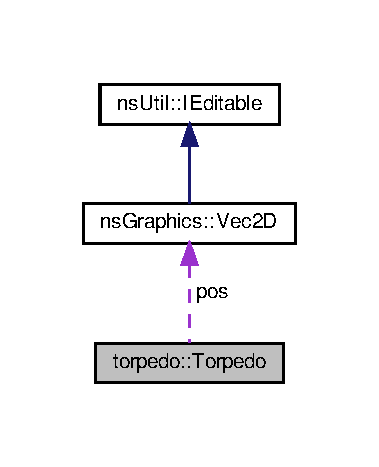
\includegraphics[width=182pt]{structtorpedo_1_1_torpedo__coll__graph}
\end{center}
\end{figure}
\subsection*{Public Member Functions}
\begin{DoxyCompactItemize}
\item 
\hyperlink{structtorpedo_1_1_torpedo_abab46a6851e2dee478c642856110661a}{Torpedo} (unsigned ent\+From, unsigned ent\+To, int ent\+PosX, int ent\+PosY)
\begin{DoxyCompactList}\small\item\em Fonction constructeur de la structure \hyperlink{structtorpedo_1_1_torpedo}{Torpedo}. \end{DoxyCompactList}\item 
void \hyperlink{structtorpedo_1_1_torpedo_a0dd38313a80970ad026919799214aee3}{update} ()
\begin{DoxyCompactList}\small\item\em Fonction de mise a jour des positions de la torpile. \end{DoxyCompactList}\item 
void \hyperlink{structtorpedo_1_1_torpedo_a00d9c4c8a5277c09d1a2f5c80bc397a7}{show} (\hyperlink{class_min_g_l}{Min\+GL} \&window)
\begin{DoxyCompactList}\small\item\em Affiche la torpille. \end{DoxyCompactList}\end{DoxyCompactItemize}
\subsection*{Public Attributes}
\begin{DoxyCompactItemize}
\item 
unsigned \hyperlink{structtorpedo_1_1_torpedo_a95c15be24a51cb7908ec34c1d1f431b2}{from}
\item 
unsigned \hyperlink{structtorpedo_1_1_torpedo_af0bdb753bc200365d66c10b47da0d3ea}{to}
\item 
\hyperlink{classns_graphics_1_1_vec2_d}{ns\+Graphics\+::\+Vec2D} \hyperlink{structtorpedo_1_1_torpedo_ae9068c94dc2a9a9484e681121526ba07}{pos}
\item 
std\+::vector$<$ unsigned long $>$ \hyperlink{structtorpedo_1_1_torpedo_a583fd4c54eb71e9af5cd29de54f12ed1}{size}
\item 
unsigned \hyperlink{structtorpedo_1_1_torpedo_aa7f3b34dce9a8062bf1fe44b5ffee0e4}{speed\+Limit}
\item 
unsigned \hyperlink{structtorpedo_1_1_torpedo_ae4d35035e6e96d86ef270474b7624b62}{speed\+Count}
\end{DoxyCompactItemize}


\subsection{Detailed Description}
Structure pour les torpilles. 

Definition at line 31 of file torpedo.\+h.



\subsection{Constructor \& Destructor Documentation}
\mbox{\Hypertarget{structtorpedo_1_1_torpedo_abab46a6851e2dee478c642856110661a}\label{structtorpedo_1_1_torpedo_abab46a6851e2dee478c642856110661a}} 
\index{torpedo\+::\+Torpedo@{torpedo\+::\+Torpedo}!Torpedo@{Torpedo}}
\index{Torpedo@{Torpedo}!torpedo\+::\+Torpedo@{torpedo\+::\+Torpedo}}
\subsubsection{\texorpdfstring{Torpedo()}{Torpedo()}}
{\footnotesize\ttfamily torpedo\+::\+Torpedo\+::\+Torpedo (\begin{DoxyParamCaption}\item[{unsigned}]{ent\+From,  }\item[{unsigned}]{ent\+To,  }\item[{int}]{ent\+PosX,  }\item[{int}]{ent\+PosY }\end{DoxyParamCaption})}



Fonction constructeur de la structure \hyperlink{structtorpedo_1_1_torpedo}{Torpedo}. 


\begin{DoxyParams}[1]{Parameters}
\mbox{\tt in}  & {\em ent\+From} & \+: Ientité du tireur (0 pour invaders, 1 pour player 1, 2 pour player 2) \\
\hline
\mbox{\tt in}  & {\em ent\+To} & \+: Sens dans lequel part la torpille (0 gauche, 1 droite) \\
\hline
\mbox{\tt in}  & {\em ent\+PosX} & \+: position X de départ de la torpille \\
\hline
\mbox{\tt in}  & {\em ent\+PosY} & \+: Position Y de départ de la torpille \\
\hline
\end{DoxyParams}


Definition at line 11 of file torpedo.\+cpp.



\subsection{Member Function Documentation}
\mbox{\Hypertarget{structtorpedo_1_1_torpedo_a00d9c4c8a5277c09d1a2f5c80bc397a7}\label{structtorpedo_1_1_torpedo_a00d9c4c8a5277c09d1a2f5c80bc397a7}} 
\index{torpedo\+::\+Torpedo@{torpedo\+::\+Torpedo}!show@{show}}
\index{show@{show}!torpedo\+::\+Torpedo@{torpedo\+::\+Torpedo}}
\subsubsection{\texorpdfstring{show()}{show()}}
{\footnotesize\ttfamily void torpedo\+::\+Torpedo\+::show (\begin{DoxyParamCaption}\item[{\hyperlink{class_min_g_l}{Min\+GL} \&}]{window }\end{DoxyParamCaption})}



Affiche la torpille. 


\begin{DoxyParams}[1]{Parameters}
\mbox{\tt in,out}  & {\em window} & \+: fenêtre de jeu \\
\hline
\end{DoxyParams}


Definition at line 38 of file torpedo.\+cpp.

\mbox{\Hypertarget{structtorpedo_1_1_torpedo_a0dd38313a80970ad026919799214aee3}\label{structtorpedo_1_1_torpedo_a0dd38313a80970ad026919799214aee3}} 
\index{torpedo\+::\+Torpedo@{torpedo\+::\+Torpedo}!update@{update}}
\index{update@{update}!torpedo\+::\+Torpedo@{torpedo\+::\+Torpedo}}
\subsubsection{\texorpdfstring{update()}{update()}}
{\footnotesize\ttfamily void torpedo\+::\+Torpedo\+::update (\begin{DoxyParamCaption}{ }\end{DoxyParamCaption})}



Fonction de mise a jour des positions de la torpile. 



Definition at line 20 of file torpedo.\+cpp.



\subsection{Member Data Documentation}
\mbox{\Hypertarget{structtorpedo_1_1_torpedo_a95c15be24a51cb7908ec34c1d1f431b2}\label{structtorpedo_1_1_torpedo_a95c15be24a51cb7908ec34c1d1f431b2}} 
\index{torpedo\+::\+Torpedo@{torpedo\+::\+Torpedo}!from@{from}}
\index{from@{from}!torpedo\+::\+Torpedo@{torpedo\+::\+Torpedo}}
\subsubsection{\texorpdfstring{from}{from}}
{\footnotesize\ttfamily unsigned torpedo\+::\+Torpedo\+::from}



Definition at line 34 of file torpedo.\+h.

\mbox{\Hypertarget{structtorpedo_1_1_torpedo_ae9068c94dc2a9a9484e681121526ba07}\label{structtorpedo_1_1_torpedo_ae9068c94dc2a9a9484e681121526ba07}} 
\index{torpedo\+::\+Torpedo@{torpedo\+::\+Torpedo}!pos@{pos}}
\index{pos@{pos}!torpedo\+::\+Torpedo@{torpedo\+::\+Torpedo}}
\subsubsection{\texorpdfstring{pos}{pos}}
{\footnotesize\ttfamily \hyperlink{classns_graphics_1_1_vec2_d}{ns\+Graphics\+::\+Vec2D} torpedo\+::\+Torpedo\+::pos}



Definition at line 36 of file torpedo.\+h.

\mbox{\Hypertarget{structtorpedo_1_1_torpedo_a583fd4c54eb71e9af5cd29de54f12ed1}\label{structtorpedo_1_1_torpedo_a583fd4c54eb71e9af5cd29de54f12ed1}} 
\index{torpedo\+::\+Torpedo@{torpedo\+::\+Torpedo}!size@{size}}
\index{size@{size}!torpedo\+::\+Torpedo@{torpedo\+::\+Torpedo}}
\subsubsection{\texorpdfstring{size}{size}}
{\footnotesize\ttfamily std\+::vector$<$unsigned long$>$ torpedo\+::\+Torpedo\+::size}



Definition at line 37 of file torpedo.\+h.

\mbox{\Hypertarget{structtorpedo_1_1_torpedo_ae4d35035e6e96d86ef270474b7624b62}\label{structtorpedo_1_1_torpedo_ae4d35035e6e96d86ef270474b7624b62}} 
\index{torpedo\+::\+Torpedo@{torpedo\+::\+Torpedo}!speed\+Count@{speed\+Count}}
\index{speed\+Count@{speed\+Count}!torpedo\+::\+Torpedo@{torpedo\+::\+Torpedo}}
\subsubsection{\texorpdfstring{speed\+Count}{speedCount}}
{\footnotesize\ttfamily unsigned torpedo\+::\+Torpedo\+::speed\+Count}



Definition at line 39 of file torpedo.\+h.

\mbox{\Hypertarget{structtorpedo_1_1_torpedo_aa7f3b34dce9a8062bf1fe44b5ffee0e4}\label{structtorpedo_1_1_torpedo_aa7f3b34dce9a8062bf1fe44b5ffee0e4}} 
\index{torpedo\+::\+Torpedo@{torpedo\+::\+Torpedo}!speed\+Limit@{speed\+Limit}}
\index{speed\+Limit@{speed\+Limit}!torpedo\+::\+Torpedo@{torpedo\+::\+Torpedo}}
\subsubsection{\texorpdfstring{speed\+Limit}{speedLimit}}
{\footnotesize\ttfamily unsigned torpedo\+::\+Torpedo\+::speed\+Limit}



Definition at line 38 of file torpedo.\+h.

\mbox{\Hypertarget{structtorpedo_1_1_torpedo_af0bdb753bc200365d66c10b47da0d3ea}\label{structtorpedo_1_1_torpedo_af0bdb753bc200365d66c10b47da0d3ea}} 
\index{torpedo\+::\+Torpedo@{torpedo\+::\+Torpedo}!to@{to}}
\index{to@{to}!torpedo\+::\+Torpedo@{torpedo\+::\+Torpedo}}
\subsubsection{\texorpdfstring{to}{to}}
{\footnotesize\ttfamily unsigned torpedo\+::\+Torpedo\+::to}



Definition at line 35 of file torpedo.\+h.



The documentation for this struct was generated from the following files\+:\begin{DoxyCompactItemize}
\item 
libs/game/entities/\hyperlink{torpedo_8h}{torpedo.\+h}\item 
src/entities/\hyperlink{torpedo_8cpp}{torpedo.\+cpp}\end{DoxyCompactItemize}

\hypertarget{classns_transition_1_1_transition}{}\section{ns\+Transition\+:\+:Transition Class Reference}
\label{classns_transition_1_1_transition}\index{ns\+Transition\+::\+Transition@{ns\+Transition\+::\+Transition}}


Une classe représentant un \hyperlink{classns_transition_1_1_transition_contract}{Transition\+Contract} en cours de lecture.  




{\ttfamily \#include $<$transition.\+h$>$}



Inheritance diagram for ns\+Transition\+:\+:Transition\+:
\nopagebreak
\begin{figure}[H]
\begin{center}
\leavevmode
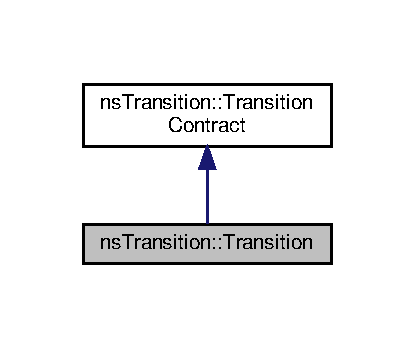
\includegraphics[width=199pt]{classns_transition_1_1_transition__inherit__graph}
\end{center}
\end{figure}


Collaboration diagram for ns\+Transition\+:\+:Transition\+:
\nopagebreak
\begin{figure}[H]
\begin{center}
\leavevmode
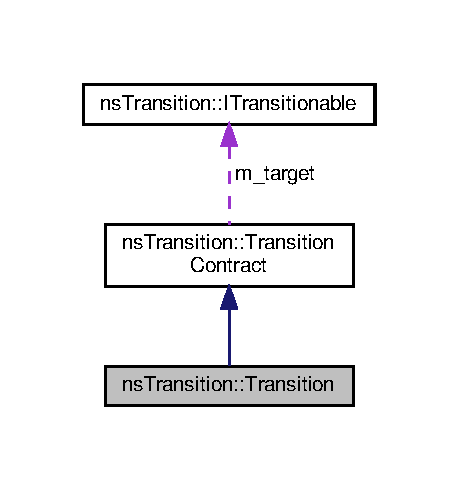
\includegraphics[width=220pt]{classns_transition_1_1_transition__coll__graph}
\end{center}
\end{figure}
\subsection*{Public Types}
\begin{DoxyCompactItemize}
\item 
enum \hyperlink{classns_transition_1_1_transition_a0bf761e331527477ce0c5e496b722a19}{Transition\+Finish\+Modes} \{ \hyperlink{classns_transition_1_1_transition_a0bf761e331527477ce0c5e496b722a19a87bacef756b461171816412a31e19ad4}{F\+I\+N\+I\+S\+H\+\_\+\+S\+T\+A\+RT}, 
\hyperlink{classns_transition_1_1_transition_a0bf761e331527477ce0c5e496b722a19a4d57dbd11ced739957f0609922a6dc9f}{F\+I\+N\+I\+S\+H\+\_\+\+C\+U\+R\+R\+E\+NT}, 
\hyperlink{classns_transition_1_1_transition_a0bf761e331527477ce0c5e496b722a19ad32a777c01bab232b51e5eeb31e2b03e}{F\+I\+N\+I\+S\+H\+\_\+\+D\+E\+S\+T\+I\+N\+A\+T\+I\+ON}
 \}\begin{DoxyCompactList}\small\item\em Transition\+Mode \+: Liste de tout les modes de fin de la \hyperlink{classns_transition_1_1_transition}{Transition}. \end{DoxyCompactList}
\end{DoxyCompactItemize}
\subsection*{Public Member Functions}
\begin{DoxyCompactItemize}
\item 
\hyperlink{classns_transition_1_1_transition_a7c3e692c43aceca5e4f716f3ae22bf05}{Transition} (const \hyperlink{classns_transition_1_1_transition_contract}{Transition\+Contract} \&contract)
\begin{DoxyCompactList}\small\item\em Constructeur pour la classe \hyperlink{classns_transition_1_1_transition}{Transition}. \end{DoxyCompactList}\item 
const \hyperlink{namespacens_transition_a260258f249f46ff9a62da721537f87af}{System\+Duration\+\_\+t} \& \hyperlink{classns_transition_1_1_transition_a616e0ef596d4e8ebb185a6cf0a685924}{get\+Elapsed} () const
\begin{DoxyCompactList}\small\item\em Retourne le temps écoulé pour cette \hyperlink{classns_transition_1_1_transition}{Transition}. \end{DoxyCompactList}\item 
void \hyperlink{classns_transition_1_1_transition_a0a8e848a50c2e05dc72800abfc6dd6ef}{set\+Elapsed} (const \hyperlink{namespacens_transition_a260258f249f46ff9a62da721537f87af}{System\+Duration\+\_\+t} \&elapsed)
\begin{DoxyCompactList}\small\item\em Définit un nouveau temps écoulé pour cette \hyperlink{classns_transition_1_1_transition}{Transition}, puis met a jour les valeurs de la cible. \end{DoxyCompactList}\item 
void \hyperlink{classns_transition_1_1_transition_abb421b44828c7b6dec60a0256a97b3d9}{add\+To\+Elapsed} (const \hyperlink{namespacens_transition_a260258f249f46ff9a62da721537f87af}{System\+Duration\+\_\+t} \&added\+Time)
\begin{DoxyCompactList}\small\item\em Rajoute une durée au temps écoulé actuel. \end{DoxyCompactList}\item 
const bool \& \hyperlink{classns_transition_1_1_transition_ab32ef25219cd2227746444ac8794266a}{is\+Reversed} () const
\begin{DoxyCompactList}\small\item\em Indique si cette \hyperlink{classns_transition_1_1_transition}{Transition} est en train de se jouer a l\textquotesingle{}envers. \end{DoxyCompactList}\item 
void \hyperlink{classns_transition_1_1_transition_a8c8c7caf7326e24ffa540093ed12f581}{finish} (const \hyperlink{classns_transition_1_1_transition_a0bf761e331527477ce0c5e496b722a19}{Transition\+Finish\+Modes} \&finish\+Mode=Transition\+Finish\+Modes\+::\+F\+I\+N\+I\+S\+H\+\_\+\+D\+E\+S\+T\+I\+N\+A\+T\+I\+ON)
\begin{DoxyCompactList}\small\item\em Marque cette \hyperlink{classns_transition_1_1_transition}{Transition} comme terminée, en utilisant le mode spécifié \end{DoxyCompactList}\item 
const bool \& \hyperlink{classns_transition_1_1_transition_ad9d358bee54825d2a8bf83e9e21e398b}{is\+Finished} () const
\begin{DoxyCompactList}\small\item\em Indique si cette \hyperlink{classns_transition_1_1_transition}{Transition} est marquée comme terminée. \end{DoxyCompactList}\end{DoxyCompactItemize}
\subsection*{Additional Inherited Members}


\subsection{Detailed Description}
Une classe représentant un \hyperlink{classns_transition_1_1_transition_contract}{Transition\+Contract} en cours de lecture. 

Definition at line 27 of file transition.\+h.



\subsection{Member Enumeration Documentation}
\mbox{\Hypertarget{classns_transition_1_1_transition_a0bf761e331527477ce0c5e496b722a19}\label{classns_transition_1_1_transition_a0bf761e331527477ce0c5e496b722a19}} 
\index{ns\+Transition\+::\+Transition@{ns\+Transition\+::\+Transition}!Transition\+Finish\+Modes@{Transition\+Finish\+Modes}}
\index{Transition\+Finish\+Modes@{Transition\+Finish\+Modes}!ns\+Transition\+::\+Transition@{ns\+Transition\+::\+Transition}}
\subsubsection{\texorpdfstring{Transition\+Finish\+Modes}{TransitionFinishModes}}
{\footnotesize\ttfamily enum \hyperlink{classns_transition_1_1_transition_a0bf761e331527477ce0c5e496b722a19}{ns\+Transition\+::\+Transition\+::\+Transition\+Finish\+Modes}}



Transition\+Mode \+: Liste de tout les modes de fin de la \hyperlink{classns_transition_1_1_transition}{Transition}. 

\begin{DoxyEnumFields}{Enumerator}
\raisebox{\heightof{T}}[0pt][0pt]{\index{F\+I\+N\+I\+S\+H\+\_\+\+S\+T\+A\+RT@{F\+I\+N\+I\+S\+H\+\_\+\+S\+T\+A\+RT}!ns\+Transition\+::\+Transition@{ns\+Transition\+::\+Transition}}\index{ns\+Transition\+::\+Transition@{ns\+Transition\+::\+Transition}!F\+I\+N\+I\+S\+H\+\_\+\+S\+T\+A\+RT@{F\+I\+N\+I\+S\+H\+\_\+\+S\+T\+A\+RT}}}\mbox{\Hypertarget{classns_transition_1_1_transition_a0bf761e331527477ce0c5e496b722a19a87bacef756b461171816412a31e19ad4}\label{classns_transition_1_1_transition_a0bf761e331527477ce0c5e496b722a19a87bacef756b461171816412a31e19ad4}} 
F\+I\+N\+I\+S\+H\+\_\+\+S\+T\+A\+RT&Ce mode de fin met les valeurs de la cible a celles de départ \\
\hline

\raisebox{\heightof{T}}[0pt][0pt]{\index{F\+I\+N\+I\+S\+H\+\_\+\+C\+U\+R\+R\+E\+NT@{F\+I\+N\+I\+S\+H\+\_\+\+C\+U\+R\+R\+E\+NT}!ns\+Transition\+::\+Transition@{ns\+Transition\+::\+Transition}}\index{ns\+Transition\+::\+Transition@{ns\+Transition\+::\+Transition}!F\+I\+N\+I\+S\+H\+\_\+\+C\+U\+R\+R\+E\+NT@{F\+I\+N\+I\+S\+H\+\_\+\+C\+U\+R\+R\+E\+NT}}}\mbox{\Hypertarget{classns_transition_1_1_transition_a0bf761e331527477ce0c5e496b722a19a4d57dbd11ced739957f0609922a6dc9f}\label{classns_transition_1_1_transition_a0bf761e331527477ce0c5e496b722a19a4d57dbd11ced739957f0609922a6dc9f}} 
F\+I\+N\+I\+S\+H\+\_\+\+C\+U\+R\+R\+E\+NT&Ce mode de fin ne touche pas aux valeurs actuelles de la cible \\
\hline

\raisebox{\heightof{T}}[0pt][0pt]{\index{F\+I\+N\+I\+S\+H\+\_\+\+D\+E\+S\+T\+I\+N\+A\+T\+I\+ON@{F\+I\+N\+I\+S\+H\+\_\+\+D\+E\+S\+T\+I\+N\+A\+T\+I\+ON}!ns\+Transition\+::\+Transition@{ns\+Transition\+::\+Transition}}\index{ns\+Transition\+::\+Transition@{ns\+Transition\+::\+Transition}!F\+I\+N\+I\+S\+H\+\_\+\+D\+E\+S\+T\+I\+N\+A\+T\+I\+ON@{F\+I\+N\+I\+S\+H\+\_\+\+D\+E\+S\+T\+I\+N\+A\+T\+I\+ON}}}\mbox{\Hypertarget{classns_transition_1_1_transition_a0bf761e331527477ce0c5e496b722a19ad32a777c01bab232b51e5eeb31e2b03e}\label{classns_transition_1_1_transition_a0bf761e331527477ce0c5e496b722a19ad32a777c01bab232b51e5eeb31e2b03e}} 
F\+I\+N\+I\+S\+H\+\_\+\+D\+E\+S\+T\+I\+N\+A\+T\+I\+ON&Ce mode de fin met les valeurs de la cible a celles d\textquotesingle{}arrivé \\
\hline

\end{DoxyEnumFields}


Definition at line 33 of file transition.\+h.



\subsection{Constructor \& Destructor Documentation}
\mbox{\Hypertarget{classns_transition_1_1_transition_a7c3e692c43aceca5e4f716f3ae22bf05}\label{classns_transition_1_1_transition_a7c3e692c43aceca5e4f716f3ae22bf05}} 
\index{ns\+Transition\+::\+Transition@{ns\+Transition\+::\+Transition}!Transition@{Transition}}
\index{Transition@{Transition}!ns\+Transition\+::\+Transition@{ns\+Transition\+::\+Transition}}
\subsubsection{\texorpdfstring{Transition()}{Transition()}}
{\footnotesize\ttfamily ns\+Transition\+::\+Transition\+::\+Transition (\begin{DoxyParamCaption}\item[{const \hyperlink{classns_transition_1_1_transition_contract}{Transition\+Contract} \&}]{contract }\end{DoxyParamCaption})}



Constructeur pour la classe \hyperlink{classns_transition_1_1_transition}{Transition}. 


\begin{DoxyParams}[1]{Parameters}
\mbox{\tt in}  & {\em contract} & \+: Contrat utilisé pour initialiser cette \hyperlink{classns_transition_1_1_transition}{Transition} \\
\hline
\end{DoxyParams}


\subsection{Member Function Documentation}
\mbox{\Hypertarget{classns_transition_1_1_transition_abb421b44828c7b6dec60a0256a97b3d9}\label{classns_transition_1_1_transition_abb421b44828c7b6dec60a0256a97b3d9}} 
\index{ns\+Transition\+::\+Transition@{ns\+Transition\+::\+Transition}!add\+To\+Elapsed@{add\+To\+Elapsed}}
\index{add\+To\+Elapsed@{add\+To\+Elapsed}!ns\+Transition\+::\+Transition@{ns\+Transition\+::\+Transition}}
\subsubsection{\texorpdfstring{add\+To\+Elapsed()}{addToElapsed()}}
{\footnotesize\ttfamily void ns\+Transition\+::\+Transition\+::add\+To\+Elapsed (\begin{DoxyParamCaption}\item[{const \hyperlink{namespacens_transition_a260258f249f46ff9a62da721537f87af}{System\+Duration\+\_\+t} \&}]{added\+Time }\end{DoxyParamCaption})}



Rajoute une durée au temps écoulé actuel. 


\begin{DoxyParams}[1]{Parameters}
\mbox{\tt in}  & {\em added\+Time} & \+: Durée a rajouter \\
\hline
\end{DoxyParams}
\mbox{\Hypertarget{classns_transition_1_1_transition_a8c8c7caf7326e24ffa540093ed12f581}\label{classns_transition_1_1_transition_a8c8c7caf7326e24ffa540093ed12f581}} 
\index{ns\+Transition\+::\+Transition@{ns\+Transition\+::\+Transition}!finish@{finish}}
\index{finish@{finish}!ns\+Transition\+::\+Transition@{ns\+Transition\+::\+Transition}}
\subsubsection{\texorpdfstring{finish()}{finish()}}
{\footnotesize\ttfamily void ns\+Transition\+::\+Transition\+::finish (\begin{DoxyParamCaption}\item[{const \hyperlink{classns_transition_1_1_transition_a0bf761e331527477ce0c5e496b722a19}{Transition\+Finish\+Modes} \&}]{finish\+Mode = {\ttfamily TransitionFinishModes\+:\+:FINISH\+\_\+DESTINATION} }\end{DoxyParamCaption})}



Marque cette \hyperlink{classns_transition_1_1_transition}{Transition} comme terminée, en utilisant le mode spécifié 


\begin{DoxyParams}[1]{Parameters}
\mbox{\tt in}  & {\em finish\+Mode} & \+: Mode utilisé pour finir cette \hyperlink{classns_transition_1_1_transition}{Transition} (Valeurs d\textquotesingle{}arrivé par défaut) \\
\hline
\end{DoxyParams}
\mbox{\Hypertarget{classns_transition_1_1_transition_a616e0ef596d4e8ebb185a6cf0a685924}\label{classns_transition_1_1_transition_a616e0ef596d4e8ebb185a6cf0a685924}} 
\index{ns\+Transition\+::\+Transition@{ns\+Transition\+::\+Transition}!get\+Elapsed@{get\+Elapsed}}
\index{get\+Elapsed@{get\+Elapsed}!ns\+Transition\+::\+Transition@{ns\+Transition\+::\+Transition}}
\subsubsection{\texorpdfstring{get\+Elapsed()}{getElapsed()}}
{\footnotesize\ttfamily const \hyperlink{namespacens_transition_a260258f249f46ff9a62da721537f87af}{System\+Duration\+\_\+t} \& ns\+Transition\+::\+Transition\+::get\+Elapsed (\begin{DoxyParamCaption}{ }\end{DoxyParamCaption}) const}



Retourne le temps écoulé pour cette \hyperlink{classns_transition_1_1_transition}{Transition}. 

\begin{DoxyReturn}{Returns}
Une référence const vers m\+\_\+elapsed 
\end{DoxyReturn}
\mbox{\Hypertarget{classns_transition_1_1_transition_ad9d358bee54825d2a8bf83e9e21e398b}\label{classns_transition_1_1_transition_ad9d358bee54825d2a8bf83e9e21e398b}} 
\index{ns\+Transition\+::\+Transition@{ns\+Transition\+::\+Transition}!is\+Finished@{is\+Finished}}
\index{is\+Finished@{is\+Finished}!ns\+Transition\+::\+Transition@{ns\+Transition\+::\+Transition}}
\subsubsection{\texorpdfstring{is\+Finished()}{isFinished()}}
{\footnotesize\ttfamily const bool \& ns\+Transition\+::\+Transition\+::is\+Finished (\begin{DoxyParamCaption}{ }\end{DoxyParamCaption}) const}



Indique si cette \hyperlink{classns_transition_1_1_transition}{Transition} est marquée comme terminée. 

\begin{DoxyReturn}{Returns}
Une référence const vers m\+\_\+finished 
\end{DoxyReturn}
\mbox{\Hypertarget{classns_transition_1_1_transition_ab32ef25219cd2227746444ac8794266a}\label{classns_transition_1_1_transition_ab32ef25219cd2227746444ac8794266a}} 
\index{ns\+Transition\+::\+Transition@{ns\+Transition\+::\+Transition}!is\+Reversed@{is\+Reversed}}
\index{is\+Reversed@{is\+Reversed}!ns\+Transition\+::\+Transition@{ns\+Transition\+::\+Transition}}
\subsubsection{\texorpdfstring{is\+Reversed()}{isReversed()}}
{\footnotesize\ttfamily const bool \& ns\+Transition\+::\+Transition\+::is\+Reversed (\begin{DoxyParamCaption}{ }\end{DoxyParamCaption}) const}



Indique si cette \hyperlink{classns_transition_1_1_transition}{Transition} est en train de se jouer a l\textquotesingle{}envers. 

\begin{DoxyReturn}{Returns}
Une référence const vers m\+\_\+reverse 
\end{DoxyReturn}
\mbox{\Hypertarget{classns_transition_1_1_transition_a0a8e848a50c2e05dc72800abfc6dd6ef}\label{classns_transition_1_1_transition_a0a8e848a50c2e05dc72800abfc6dd6ef}} 
\index{ns\+Transition\+::\+Transition@{ns\+Transition\+::\+Transition}!set\+Elapsed@{set\+Elapsed}}
\index{set\+Elapsed@{set\+Elapsed}!ns\+Transition\+::\+Transition@{ns\+Transition\+::\+Transition}}
\subsubsection{\texorpdfstring{set\+Elapsed()}{setElapsed()}}
{\footnotesize\ttfamily void ns\+Transition\+::\+Transition\+::set\+Elapsed (\begin{DoxyParamCaption}\item[{const \hyperlink{namespacens_transition_a260258f249f46ff9a62da721537f87af}{System\+Duration\+\_\+t} \&}]{elapsed }\end{DoxyParamCaption})}



Définit un nouveau temps écoulé pour cette \hyperlink{classns_transition_1_1_transition}{Transition}, puis met a jour les valeurs de la cible. 


\begin{DoxyParams}[1]{Parameters}
\mbox{\tt in}  & {\em elapsed} & \+: Nouveau temps écoulé \\
\hline
\end{DoxyParams}


The documentation for this class was generated from the following file\+:\begin{DoxyCompactItemize}
\item 
libs/mingl/transition/\hyperlink{transition_8h}{transition.\+h}\end{DoxyCompactItemize}

\hypertarget{classns_transition_1_1_transition_contract}{}\section{ns\+Transition\+:\+:Transition\+Contract Class Reference}
\label{classns_transition_1_1_transition_contract}\index{ns\+Transition\+::\+Transition\+Contract@{ns\+Transition\+::\+Transition\+Contract}}


Une classe contenant des paramètres pour créer une transition.  




{\ttfamily \#include $<$transition\+\_\+contract.\+h$>$}



Inheritance diagram for ns\+Transition\+:\+:Transition\+Contract\+:
\nopagebreak
\begin{figure}[H]
\begin{center}
\leavevmode
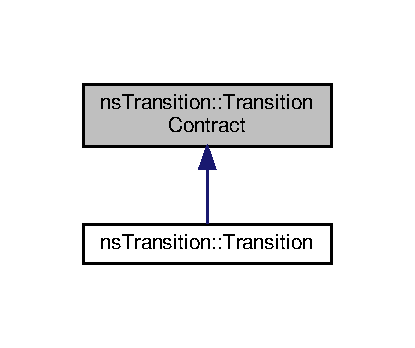
\includegraphics[width=199pt]{classns_transition_1_1_transition_contract__inherit__graph}
\end{center}
\end{figure}


Collaboration diagram for ns\+Transition\+:\+:Transition\+Contract\+:
\nopagebreak
\begin{figure}[H]
\begin{center}
\leavevmode
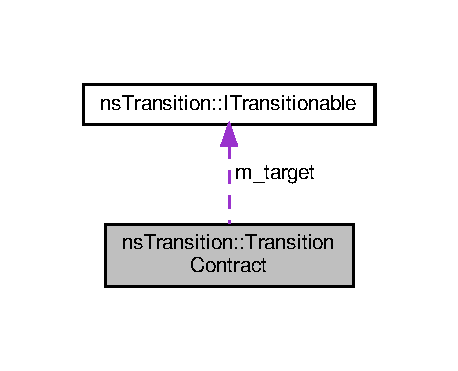
\includegraphics[width=220pt]{classns_transition_1_1_transition_contract__coll__graph}
\end{center}
\end{figure}
\subsection*{Public Types}
\begin{DoxyCompactItemize}
\item 
enum \hyperlink{classns_transition_1_1_transition_contract_a40118ebf3c1a0a486934ce2b9ddc3edb}{Transition\+Mode} \{ \hyperlink{classns_transition_1_1_transition_contract_a40118ebf3c1a0a486934ce2b9ddc3edba8e6b597d9cc193da6eb40a6be5dc544b}{M\+O\+D\+E\+\_\+\+F\+I\+N\+I\+TE}, 
\hyperlink{classns_transition_1_1_transition_contract_a40118ebf3c1a0a486934ce2b9ddc3edbada40ee822d94803e81878d415e46ef6a}{M\+O\+D\+E\+\_\+\+F\+I\+N\+I\+T\+E\+\_\+\+R\+E\+V\+E\+R\+SE}, 
\hyperlink{classns_transition_1_1_transition_contract_a40118ebf3c1a0a486934ce2b9ddc3edbaaf7f662702b3f37a41b8cfb86598f857}{M\+O\+D\+E\+\_\+\+L\+O\+OP}, 
\hyperlink{classns_transition_1_1_transition_contract_a40118ebf3c1a0a486934ce2b9ddc3edba5aa6e1fbf9670aa9ecd96beff2ba6abb}{M\+O\+D\+E\+\_\+\+L\+O\+O\+P\+\_\+\+S\+M\+O\+O\+TH}
 \}\begin{DoxyCompactList}\small\item\em Transition\+Mode \+: Liste de tout les modes de transition. \end{DoxyCompactList}
\end{DoxyCompactItemize}
\subsection*{Public Member Functions}
\begin{DoxyCompactItemize}
\item 
\hyperlink{classns_transition_1_1_transition_contract_a8ec4ef83c08901c9b93cec5eb0bfd06b}{Transition\+Contract} (\hyperlink{classns_transition_1_1_i_transitionable}{I\+Transitionable} \&target, const int \&id, const \hyperlink{namespacens_transition_a260258f249f46ff9a62da721537f87af}{System\+Duration\+\_\+t} \&duration, const std\+::vector$<$ float $>$ \&destination, const \hyperlink{namespacens_transition_a260258f249f46ff9a62da721537f87af}{System\+Duration\+\_\+t} \&delay=std\+::chrono\+::seconds\+::zero(), const \hyperlink{classns_transition_1_1_transition_contract_a40118ebf3c1a0a486934ce2b9ddc3edb}{Transition\+Mode} \&transition\+Mode=Transition\+Mode\+::\+M\+O\+D\+E\+\_\+\+F\+I\+N\+I\+TE)
\begin{DoxyCompactList}\small\item\em Constructeur pour la classe \hyperlink{classns_transition_1_1_transition_contract}{Transition\+Contract}. \end{DoxyCompactList}\item 
const int \& \hyperlink{classns_transition_1_1_transition_contract_a34a594d05171628bca81120c768c86b9}{get\+Id} () const
\begin{DoxyCompactList}\small\item\em Retourne l\textquotesingle{}ID de transition, utilisé par la cible pour connaitre les valeurs a utiliser. \end{DoxyCompactList}\item 
const \hyperlink{classns_transition_1_1_i_transitionable}{I\+Transitionable} \& \hyperlink{classns_transition_1_1_transition_contract_a464b06c739e50a374c4d11509cf6e5ee}{get\+Target} () const
\begin{DoxyCompactList}\small\item\em Retourne la cible de transition. \end{DoxyCompactList}\item 
const \hyperlink{classns_transition_1_1_transition_contract_a40118ebf3c1a0a486934ce2b9ddc3edb}{Transition\+Mode} \& \hyperlink{classns_transition_1_1_transition_contract_ad5d6524d7e2eeddf9f06204b8245c484}{get\+Transition\+Mode} () const
\begin{DoxyCompactList}\small\item\em Retourne le mode de transition. \end{DoxyCompactList}\item 
const std\+::vector$<$ float $>$ \& \hyperlink{classns_transition_1_1_transition_contract_a8dc505c54df5d1f09a482a1b56676cd4}{get\+Beginning} () const
\begin{DoxyCompactList}\small\item\em Retourne les valeurs de départ. \end{DoxyCompactList}\item 
const std\+::vector$<$ float $>$ \& \hyperlink{classns_transition_1_1_transition_contract_ae4ce420a4376e1d372efb3fd046410df}{get\+Destination} () const
\begin{DoxyCompactList}\small\item\em Retourne les valeurs d\textquotesingle{}arrivée. \end{DoxyCompactList}\item 
const \hyperlink{namespacens_transition_a260258f249f46ff9a62da721537f87af}{System\+Duration\+\_\+t} \& \hyperlink{classns_transition_1_1_transition_contract_a9b900986c8f271729f99c88fa1b0a5e1}{get\+Duration} () const
\begin{DoxyCompactList}\small\item\em Retourne la durée de la transition. \end{DoxyCompactList}\item 
void \hyperlink{classns_transition_1_1_transition_contract_a8f1ebafd9966553678fd7845f35bac33}{set\+Destination\+Callback} (const std\+::function$<$ void()$>$ \&callback)
\begin{DoxyCompactList}\small\item\em Définit la fonction de callback a appeler quand la transition est achevée. \end{DoxyCompactList}\end{DoxyCompactItemize}
\subsection*{Protected Attributes}
\begin{DoxyCompactItemize}
\item 
const int \hyperlink{classns_transition_1_1_transition_contract_a48e1b58bc26cb8b6167fb6b76911c941}{m\+\_\+id}
\begin{DoxyCompactList}\small\item\em m\+\_\+id \+: L\textquotesingle{}ID de la transition \end{DoxyCompactList}\item 
\hyperlink{classns_transition_1_1_i_transitionable}{I\+Transitionable} \& \hyperlink{classns_transition_1_1_transition_contract_a1066c3c1526a519276b75a4f4c5206b2}{m\+\_\+target}
\begin{DoxyCompactList}\small\item\em m\+\_\+target \+: Une référence vers une instance d\textquotesingle{}une classe dérivée d\textquotesingle{}\hyperlink{classns_transition_1_1_i_transitionable}{I\+Transitionable} \end{DoxyCompactList}\item 
const \hyperlink{classns_transition_1_1_transition_contract_a40118ebf3c1a0a486934ce2b9ddc3edb}{Transition\+Mode} \hyperlink{classns_transition_1_1_transition_contract_a9634edf746d8605e78ae30f7a0e6efd3}{m\+\_\+transition\+Mode}
\begin{DoxyCompactList}\small\item\em m\+\_\+transition\+Mode \+: Le mode de transition \end{DoxyCompactList}\item 
std\+::vector$<$ float $>$ \hyperlink{classns_transition_1_1_transition_contract_a5f804f0f4cc00d48e139ff93c5469954}{m\+\_\+beginning}
\begin{DoxyCompactList}\small\item\em m\+\_\+beginning \+: Contient les valeurs de départ \end{DoxyCompactList}\item 
const std\+::vector$<$ float $>$ \hyperlink{classns_transition_1_1_transition_contract_adc660e53bde2e552bb4148ac7abc4e42}{m\+\_\+destination}
\begin{DoxyCompactList}\small\item\em m\+\_\+destination \+: Contient les valeurs d\textquotesingle{}arrivées \end{DoxyCompactList}\item 
\hyperlink{namespacens_transition_a260258f249f46ff9a62da721537f87af}{System\+Duration\+\_\+t} \hyperlink{classns_transition_1_1_transition_contract_a0c8ac97863022965d6ac0539d972c325}{m\+\_\+duration}
\begin{DoxyCompactList}\small\item\em m\+\_\+duration \+: La durée de la transition \end{DoxyCompactList}\item 
\hyperlink{namespacens_transition_a260258f249f46ff9a62da721537f87af}{System\+Duration\+\_\+t} \hyperlink{classns_transition_1_1_transition_contract_a5c317b573104f3d3c9caafbc3014ac16}{m\+\_\+delay}
\begin{DoxyCompactList}\small\item\em m\+\_\+delay \+: Délai a attendre avant que la transition ne démarre \end{DoxyCompactList}\item 
std\+::function$<$ void()$>$ \hyperlink{classns_transition_1_1_transition_contract_ac95072df084f1edbd63479c68228b9d6}{m\+\_\+destination\+Callback}
\begin{DoxyCompactList}\small\item\em m\+\_\+duration \+: Un pointeur vers la fonction a appeler une fois la transition achevée \end{DoxyCompactList}\end{DoxyCompactItemize}


\subsection{Detailed Description}
Une classe contenant des paramètres pour créer une transition. 

Definition at line 27 of file transition\+\_\+contract.\+h.



\subsection{Member Enumeration Documentation}
\mbox{\Hypertarget{classns_transition_1_1_transition_contract_a40118ebf3c1a0a486934ce2b9ddc3edb}\label{classns_transition_1_1_transition_contract_a40118ebf3c1a0a486934ce2b9ddc3edb}} 
\index{ns\+Transition\+::\+Transition\+Contract@{ns\+Transition\+::\+Transition\+Contract}!Transition\+Mode@{Transition\+Mode}}
\index{Transition\+Mode@{Transition\+Mode}!ns\+Transition\+::\+Transition\+Contract@{ns\+Transition\+::\+Transition\+Contract}}
\subsubsection{\texorpdfstring{Transition\+Mode}{TransitionMode}}
{\footnotesize\ttfamily enum \hyperlink{classns_transition_1_1_transition_contract_a40118ebf3c1a0a486934ce2b9ddc3edb}{ns\+Transition\+::\+Transition\+Contract\+::\+Transition\+Mode}}



Transition\+Mode \+: Liste de tout les modes de transition. 

\begin{DoxyEnumFields}{Enumerator}
\raisebox{\heightof{T}}[0pt][0pt]{\index{M\+O\+D\+E\+\_\+\+F\+I\+N\+I\+TE@{M\+O\+D\+E\+\_\+\+F\+I\+N\+I\+TE}!ns\+Transition\+::\+Transition\+Contract@{ns\+Transition\+::\+Transition\+Contract}}\index{ns\+Transition\+::\+Transition\+Contract@{ns\+Transition\+::\+Transition\+Contract}!M\+O\+D\+E\+\_\+\+F\+I\+N\+I\+TE@{M\+O\+D\+E\+\_\+\+F\+I\+N\+I\+TE}}}\mbox{\Hypertarget{classns_transition_1_1_transition_contract_a40118ebf3c1a0a486934ce2b9ddc3edba8e6b597d9cc193da6eb40a6be5dc544b}\label{classns_transition_1_1_transition_contract_a40118ebf3c1a0a486934ce2b9ddc3edba8e6b597d9cc193da6eb40a6be5dc544b}} 
M\+O\+D\+E\+\_\+\+F\+I\+N\+I\+TE&Ce mode marque la \hyperlink{classns_transition_1_1_transition}{Transition} comme terminée une fois achevée \\
\hline

\raisebox{\heightof{T}}[0pt][0pt]{\index{M\+O\+D\+E\+\_\+\+F\+I\+N\+I\+T\+E\+\_\+\+R\+E\+V\+E\+R\+SE@{M\+O\+D\+E\+\_\+\+F\+I\+N\+I\+T\+E\+\_\+\+R\+E\+V\+E\+R\+SE}!ns\+Transition\+::\+Transition\+Contract@{ns\+Transition\+::\+Transition\+Contract}}\index{ns\+Transition\+::\+Transition\+Contract@{ns\+Transition\+::\+Transition\+Contract}!M\+O\+D\+E\+\_\+\+F\+I\+N\+I\+T\+E\+\_\+\+R\+E\+V\+E\+R\+SE@{M\+O\+D\+E\+\_\+\+F\+I\+N\+I\+T\+E\+\_\+\+R\+E\+V\+E\+R\+SE}}}\mbox{\Hypertarget{classns_transition_1_1_transition_contract_a40118ebf3c1a0a486934ce2b9ddc3edbada40ee822d94803e81878d415e46ef6a}\label{classns_transition_1_1_transition_contract_a40118ebf3c1a0a486934ce2b9ddc3edbada40ee822d94803e81878d415e46ef6a}} 
M\+O\+D\+E\+\_\+\+F\+I\+N\+I\+T\+E\+\_\+\+R\+E\+V\+E\+R\+SE&Ce mode va jouer la \hyperlink{classns_transition_1_1_transition}{Transition} a l\textquotesingle{}envers une fois achevée, puis marquer la \hyperlink{classns_transition_1_1_transition}{Transition} comme étant terminée \\
\hline

\raisebox{\heightof{T}}[0pt][0pt]{\index{M\+O\+D\+E\+\_\+\+L\+O\+OP@{M\+O\+D\+E\+\_\+\+L\+O\+OP}!ns\+Transition\+::\+Transition\+Contract@{ns\+Transition\+::\+Transition\+Contract}}\index{ns\+Transition\+::\+Transition\+Contract@{ns\+Transition\+::\+Transition\+Contract}!M\+O\+D\+E\+\_\+\+L\+O\+OP@{M\+O\+D\+E\+\_\+\+L\+O\+OP}}}\mbox{\Hypertarget{classns_transition_1_1_transition_contract_a40118ebf3c1a0a486934ce2b9ddc3edbaaf7f662702b3f37a41b8cfb86598f857}\label{classns_transition_1_1_transition_contract_a40118ebf3c1a0a486934ce2b9ddc3edbaaf7f662702b3f37a41b8cfb86598f857}} 
M\+O\+D\+E\+\_\+\+L\+O\+OP&Ce mode va définir les valeurs de départ a la cible une fois la \hyperlink{classns_transition_1_1_transition}{Transition} achevée, puis se rejouer en boucle \\
\hline

\raisebox{\heightof{T}}[0pt][0pt]{\index{M\+O\+D\+E\+\_\+\+L\+O\+O\+P\+\_\+\+S\+M\+O\+O\+TH@{M\+O\+D\+E\+\_\+\+L\+O\+O\+P\+\_\+\+S\+M\+O\+O\+TH}!ns\+Transition\+::\+Transition\+Contract@{ns\+Transition\+::\+Transition\+Contract}}\index{ns\+Transition\+::\+Transition\+Contract@{ns\+Transition\+::\+Transition\+Contract}!M\+O\+D\+E\+\_\+\+L\+O\+O\+P\+\_\+\+S\+M\+O\+O\+TH@{M\+O\+D\+E\+\_\+\+L\+O\+O\+P\+\_\+\+S\+M\+O\+O\+TH}}}\mbox{\Hypertarget{classns_transition_1_1_transition_contract_a40118ebf3c1a0a486934ce2b9ddc3edba5aa6e1fbf9670aa9ecd96beff2ba6abb}\label{classns_transition_1_1_transition_contract_a40118ebf3c1a0a486934ce2b9ddc3edba5aa6e1fbf9670aa9ecd96beff2ba6abb}} 
M\+O\+D\+E\+\_\+\+L\+O\+O\+P\+\_\+\+S\+M\+O\+O\+TH&Ce mode va jouer la \hyperlink{classns_transition_1_1_transition}{Transition} a l\textquotesingle{}envers une fois achevée, puis se rejouer en boucle \\
\hline

\end{DoxyEnumFields}


Definition at line 33 of file transition\+\_\+contract.\+h.



\subsection{Constructor \& Destructor Documentation}
\mbox{\Hypertarget{classns_transition_1_1_transition_contract_a8ec4ef83c08901c9b93cec5eb0bfd06b}\label{classns_transition_1_1_transition_contract_a8ec4ef83c08901c9b93cec5eb0bfd06b}} 
\index{ns\+Transition\+::\+Transition\+Contract@{ns\+Transition\+::\+Transition\+Contract}!Transition\+Contract@{Transition\+Contract}}
\index{Transition\+Contract@{Transition\+Contract}!ns\+Transition\+::\+Transition\+Contract@{ns\+Transition\+::\+Transition\+Contract}}
\subsubsection{\texorpdfstring{Transition\+Contract()}{TransitionContract()}}
{\footnotesize\ttfamily ns\+Transition\+::\+Transition\+Contract\+::\+Transition\+Contract (\begin{DoxyParamCaption}\item[{\hyperlink{classns_transition_1_1_i_transitionable}{I\+Transitionable} \&}]{target,  }\item[{const int \&}]{id,  }\item[{const \hyperlink{namespacens_transition_a260258f249f46ff9a62da721537f87af}{System\+Duration\+\_\+t} \&}]{duration,  }\item[{const std\+::vector$<$ float $>$ \&}]{destination,  }\item[{const \hyperlink{namespacens_transition_a260258f249f46ff9a62da721537f87af}{System\+Duration\+\_\+t} \&}]{delay = {\ttfamily std\+:\+:chrono\+:\+:seconds\+:\+:zero()},  }\item[{const \hyperlink{classns_transition_1_1_transition_contract_a40118ebf3c1a0a486934ce2b9ddc3edb}{Transition\+Mode} \&}]{transition\+Mode = {\ttfamily TransitionMode\+:\+:MODE\+\_\+FINITE} }\end{DoxyParamCaption})}



Constructeur pour la classe \hyperlink{classns_transition_1_1_transition_contract}{Transition\+Contract}. 


\begin{DoxyParams}[1]{Parameters}
\mbox{\tt in,out}  & {\em target} & \+: Une référence vers une classe dérivée d\textquotesingle{}\hyperlink{classns_transition_1_1_i_transitionable}{I\+Transitionable} qui sera la cible \\
\hline
\mbox{\tt in}  & {\em id} & \+: L\textquotesingle{}ID de la transition a appliquer \\
\hline
\mbox{\tt in}  & {\em duration} & \+: La durée de la transition \\
\hline
\mbox{\tt in}  & {\em destination} & \+: Les valeurs d\textquotesingle{}arrivée \\
\hline
\mbox{\tt in}  & {\em delay} & \+: Délai avant que la transition commence (Zéro par défaut) \\
\hline
\mbox{\tt in}  & {\em transition\+Mode} & \+: Mode de transition (\hyperlink{classns_transition_1_1_transition}{Transition} finie par défaut) \\
\hline
\end{DoxyParams}


\subsection{Member Function Documentation}
\mbox{\Hypertarget{classns_transition_1_1_transition_contract_a8dc505c54df5d1f09a482a1b56676cd4}\label{classns_transition_1_1_transition_contract_a8dc505c54df5d1f09a482a1b56676cd4}} 
\index{ns\+Transition\+::\+Transition\+Contract@{ns\+Transition\+::\+Transition\+Contract}!get\+Beginning@{get\+Beginning}}
\index{get\+Beginning@{get\+Beginning}!ns\+Transition\+::\+Transition\+Contract@{ns\+Transition\+::\+Transition\+Contract}}
\subsubsection{\texorpdfstring{get\+Beginning()}{getBeginning()}}
{\footnotesize\ttfamily const std\+::vector$<$ float $>$ \& ns\+Transition\+::\+Transition\+Contract\+::get\+Beginning (\begin{DoxyParamCaption}{ }\end{DoxyParamCaption}) const}



Retourne les valeurs de départ. 

\begin{DoxyReturn}{Returns}
Une référence const vers m\+\_\+beginning 
\end{DoxyReturn}
\mbox{\Hypertarget{classns_transition_1_1_transition_contract_ae4ce420a4376e1d372efb3fd046410df}\label{classns_transition_1_1_transition_contract_ae4ce420a4376e1d372efb3fd046410df}} 
\index{ns\+Transition\+::\+Transition\+Contract@{ns\+Transition\+::\+Transition\+Contract}!get\+Destination@{get\+Destination}}
\index{get\+Destination@{get\+Destination}!ns\+Transition\+::\+Transition\+Contract@{ns\+Transition\+::\+Transition\+Contract}}
\subsubsection{\texorpdfstring{get\+Destination()}{getDestination()}}
{\footnotesize\ttfamily const std\+::vector$<$ float $>$ \& ns\+Transition\+::\+Transition\+Contract\+::get\+Destination (\begin{DoxyParamCaption}{ }\end{DoxyParamCaption}) const}



Retourne les valeurs d\textquotesingle{}arrivée. 

\begin{DoxyReturn}{Returns}
Une référence const vers m\+\_\+destination 
\end{DoxyReturn}
\mbox{\Hypertarget{classns_transition_1_1_transition_contract_a9b900986c8f271729f99c88fa1b0a5e1}\label{classns_transition_1_1_transition_contract_a9b900986c8f271729f99c88fa1b0a5e1}} 
\index{ns\+Transition\+::\+Transition\+Contract@{ns\+Transition\+::\+Transition\+Contract}!get\+Duration@{get\+Duration}}
\index{get\+Duration@{get\+Duration}!ns\+Transition\+::\+Transition\+Contract@{ns\+Transition\+::\+Transition\+Contract}}
\subsubsection{\texorpdfstring{get\+Duration()}{getDuration()}}
{\footnotesize\ttfamily const \hyperlink{namespacens_transition_a260258f249f46ff9a62da721537f87af}{System\+Duration\+\_\+t} \& ns\+Transition\+::\+Transition\+Contract\+::get\+Duration (\begin{DoxyParamCaption}{ }\end{DoxyParamCaption}) const}



Retourne la durée de la transition. 

\begin{DoxyReturn}{Returns}
Une référence const vers m\+\_\+duration 
\end{DoxyReturn}
\mbox{\Hypertarget{classns_transition_1_1_transition_contract_a34a594d05171628bca81120c768c86b9}\label{classns_transition_1_1_transition_contract_a34a594d05171628bca81120c768c86b9}} 
\index{ns\+Transition\+::\+Transition\+Contract@{ns\+Transition\+::\+Transition\+Contract}!get\+Id@{get\+Id}}
\index{get\+Id@{get\+Id}!ns\+Transition\+::\+Transition\+Contract@{ns\+Transition\+::\+Transition\+Contract}}
\subsubsection{\texorpdfstring{get\+Id()}{getId()}}
{\footnotesize\ttfamily const int \& ns\+Transition\+::\+Transition\+Contract\+::get\+Id (\begin{DoxyParamCaption}{ }\end{DoxyParamCaption}) const}



Retourne l\textquotesingle{}ID de transition, utilisé par la cible pour connaitre les valeurs a utiliser. 

\begin{DoxyReturn}{Returns}
Une référence const vers m\+\_\+id 
\end{DoxyReturn}
\mbox{\Hypertarget{classns_transition_1_1_transition_contract_a464b06c739e50a374c4d11509cf6e5ee}\label{classns_transition_1_1_transition_contract_a464b06c739e50a374c4d11509cf6e5ee}} 
\index{ns\+Transition\+::\+Transition\+Contract@{ns\+Transition\+::\+Transition\+Contract}!get\+Target@{get\+Target}}
\index{get\+Target@{get\+Target}!ns\+Transition\+::\+Transition\+Contract@{ns\+Transition\+::\+Transition\+Contract}}
\subsubsection{\texorpdfstring{get\+Target()}{getTarget()}}
{\footnotesize\ttfamily const \hyperlink{classns_transition_1_1_i_transitionable}{I\+Transitionable} \& ns\+Transition\+::\+Transition\+Contract\+::get\+Target (\begin{DoxyParamCaption}{ }\end{DoxyParamCaption}) const}



Retourne la cible de transition. 

\begin{DoxyReturn}{Returns}
Une référence const vers m\+\_\+target 
\end{DoxyReturn}
\mbox{\Hypertarget{classns_transition_1_1_transition_contract_ad5d6524d7e2eeddf9f06204b8245c484}\label{classns_transition_1_1_transition_contract_ad5d6524d7e2eeddf9f06204b8245c484}} 
\index{ns\+Transition\+::\+Transition\+Contract@{ns\+Transition\+::\+Transition\+Contract}!get\+Transition\+Mode@{get\+Transition\+Mode}}
\index{get\+Transition\+Mode@{get\+Transition\+Mode}!ns\+Transition\+::\+Transition\+Contract@{ns\+Transition\+::\+Transition\+Contract}}
\subsubsection{\texorpdfstring{get\+Transition\+Mode()}{getTransitionMode()}}
{\footnotesize\ttfamily const \hyperlink{classns_transition_1_1_transition_contract_a40118ebf3c1a0a486934ce2b9ddc3edb}{Transition\+Mode} \& ns\+Transition\+::\+Transition\+Contract\+::get\+Transition\+Mode (\begin{DoxyParamCaption}{ }\end{DoxyParamCaption}) const}



Retourne le mode de transition. 

\begin{DoxyReturn}{Returns}
Une référence const vers m\+\_\+transition\+Mode 
\end{DoxyReturn}
\mbox{\Hypertarget{classns_transition_1_1_transition_contract_a8f1ebafd9966553678fd7845f35bac33}\label{classns_transition_1_1_transition_contract_a8f1ebafd9966553678fd7845f35bac33}} 
\index{ns\+Transition\+::\+Transition\+Contract@{ns\+Transition\+::\+Transition\+Contract}!set\+Destination\+Callback@{set\+Destination\+Callback}}
\index{set\+Destination\+Callback@{set\+Destination\+Callback}!ns\+Transition\+::\+Transition\+Contract@{ns\+Transition\+::\+Transition\+Contract}}
\subsubsection{\texorpdfstring{set\+Destination\+Callback()}{setDestinationCallback()}}
{\footnotesize\ttfamily void ns\+Transition\+::\+Transition\+Contract\+::set\+Destination\+Callback (\begin{DoxyParamCaption}\item[{const std\+::function$<$ void()$>$ \&}]{callback }\end{DoxyParamCaption})}



Définit la fonction de callback a appeler quand la transition est achevée. 


\begin{DoxyParams}[1]{Parameters}
\mbox{\tt in}  & {\em callback} & \+: La fonction a appeler \\
\hline
\end{DoxyParams}


\subsection{Member Data Documentation}
\mbox{\Hypertarget{classns_transition_1_1_transition_contract_a5f804f0f4cc00d48e139ff93c5469954}\label{classns_transition_1_1_transition_contract_a5f804f0f4cc00d48e139ff93c5469954}} 
\index{ns\+Transition\+::\+Transition\+Contract@{ns\+Transition\+::\+Transition\+Contract}!m\+\_\+beginning@{m\+\_\+beginning}}
\index{m\+\_\+beginning@{m\+\_\+beginning}!ns\+Transition\+::\+Transition\+Contract@{ns\+Transition\+::\+Transition\+Contract}}
\subsubsection{\texorpdfstring{m\+\_\+beginning}{m\_beginning}}
{\footnotesize\ttfamily std\+::vector$<$float$>$ ns\+Transition\+::\+Transition\+Contract\+::m\+\_\+beginning\hspace{0.3cm}{\ttfamily [protected]}}



m\+\_\+beginning \+: Contient les valeurs de départ 



Definition at line 133 of file transition\+\_\+contract.\+h.

\mbox{\Hypertarget{classns_transition_1_1_transition_contract_a5c317b573104f3d3c9caafbc3014ac16}\label{classns_transition_1_1_transition_contract_a5c317b573104f3d3c9caafbc3014ac16}} 
\index{ns\+Transition\+::\+Transition\+Contract@{ns\+Transition\+::\+Transition\+Contract}!m\+\_\+delay@{m\+\_\+delay}}
\index{m\+\_\+delay@{m\+\_\+delay}!ns\+Transition\+::\+Transition\+Contract@{ns\+Transition\+::\+Transition\+Contract}}
\subsubsection{\texorpdfstring{m\+\_\+delay}{m\_delay}}
{\footnotesize\ttfamily \hyperlink{namespacens_transition_a260258f249f46ff9a62da721537f87af}{System\+Duration\+\_\+t} ns\+Transition\+::\+Transition\+Contract\+::m\+\_\+delay\hspace{0.3cm}{\ttfamily [protected]}}



m\+\_\+delay \+: Délai a attendre avant que la transition ne démarre 



Definition at line 148 of file transition\+\_\+contract.\+h.

\mbox{\Hypertarget{classns_transition_1_1_transition_contract_adc660e53bde2e552bb4148ac7abc4e42}\label{classns_transition_1_1_transition_contract_adc660e53bde2e552bb4148ac7abc4e42}} 
\index{ns\+Transition\+::\+Transition\+Contract@{ns\+Transition\+::\+Transition\+Contract}!m\+\_\+destination@{m\+\_\+destination}}
\index{m\+\_\+destination@{m\+\_\+destination}!ns\+Transition\+::\+Transition\+Contract@{ns\+Transition\+::\+Transition\+Contract}}
\subsubsection{\texorpdfstring{m\+\_\+destination}{m\_destination}}
{\footnotesize\ttfamily const std\+::vector$<$float$>$ ns\+Transition\+::\+Transition\+Contract\+::m\+\_\+destination\hspace{0.3cm}{\ttfamily [protected]}}



m\+\_\+destination \+: Contient les valeurs d\textquotesingle{}arrivées 



Definition at line 138 of file transition\+\_\+contract.\+h.

\mbox{\Hypertarget{classns_transition_1_1_transition_contract_ac95072df084f1edbd63479c68228b9d6}\label{classns_transition_1_1_transition_contract_ac95072df084f1edbd63479c68228b9d6}} 
\index{ns\+Transition\+::\+Transition\+Contract@{ns\+Transition\+::\+Transition\+Contract}!m\+\_\+destination\+Callback@{m\+\_\+destination\+Callback}}
\index{m\+\_\+destination\+Callback@{m\+\_\+destination\+Callback}!ns\+Transition\+::\+Transition\+Contract@{ns\+Transition\+::\+Transition\+Contract}}
\subsubsection{\texorpdfstring{m\+\_\+destination\+Callback}{m\_destinationCallback}}
{\footnotesize\ttfamily std\+::function$<$void()$>$ ns\+Transition\+::\+Transition\+Contract\+::m\+\_\+destination\+Callback\hspace{0.3cm}{\ttfamily [protected]}}



m\+\_\+duration \+: Un pointeur vers la fonction a appeler une fois la transition achevée 



Definition at line 153 of file transition\+\_\+contract.\+h.

\mbox{\Hypertarget{classns_transition_1_1_transition_contract_a0c8ac97863022965d6ac0539d972c325}\label{classns_transition_1_1_transition_contract_a0c8ac97863022965d6ac0539d972c325}} 
\index{ns\+Transition\+::\+Transition\+Contract@{ns\+Transition\+::\+Transition\+Contract}!m\+\_\+duration@{m\+\_\+duration}}
\index{m\+\_\+duration@{m\+\_\+duration}!ns\+Transition\+::\+Transition\+Contract@{ns\+Transition\+::\+Transition\+Contract}}
\subsubsection{\texorpdfstring{m\+\_\+duration}{m\_duration}}
{\footnotesize\ttfamily \hyperlink{namespacens_transition_a260258f249f46ff9a62da721537f87af}{System\+Duration\+\_\+t} ns\+Transition\+::\+Transition\+Contract\+::m\+\_\+duration\hspace{0.3cm}{\ttfamily [protected]}}



m\+\_\+duration \+: La durée de la transition 



Definition at line 143 of file transition\+\_\+contract.\+h.

\mbox{\Hypertarget{classns_transition_1_1_transition_contract_a48e1b58bc26cb8b6167fb6b76911c941}\label{classns_transition_1_1_transition_contract_a48e1b58bc26cb8b6167fb6b76911c941}} 
\index{ns\+Transition\+::\+Transition\+Contract@{ns\+Transition\+::\+Transition\+Contract}!m\+\_\+id@{m\+\_\+id}}
\index{m\+\_\+id@{m\+\_\+id}!ns\+Transition\+::\+Transition\+Contract@{ns\+Transition\+::\+Transition\+Contract}}
\subsubsection{\texorpdfstring{m\+\_\+id}{m\_id}}
{\footnotesize\ttfamily const int ns\+Transition\+::\+Transition\+Contract\+::m\+\_\+id\hspace{0.3cm}{\ttfamily [protected]}}



m\+\_\+id \+: L\textquotesingle{}ID de la transition 

Ceci est seulement utile pour la cible, car lui seul sait a quel ID correspond quelles valeurs. Ainsi, l\textquotesingle{}ID n\textquotesingle{}est jamais utilisée directement par la transition et est seulement passée a la cible. 

Definition at line 114 of file transition\+\_\+contract.\+h.

\mbox{\Hypertarget{classns_transition_1_1_transition_contract_a1066c3c1526a519276b75a4f4c5206b2}\label{classns_transition_1_1_transition_contract_a1066c3c1526a519276b75a4f4c5206b2}} 
\index{ns\+Transition\+::\+Transition\+Contract@{ns\+Transition\+::\+Transition\+Contract}!m\+\_\+target@{m\+\_\+target}}
\index{m\+\_\+target@{m\+\_\+target}!ns\+Transition\+::\+Transition\+Contract@{ns\+Transition\+::\+Transition\+Contract}}
\subsubsection{\texorpdfstring{m\+\_\+target}{m\_target}}
{\footnotesize\ttfamily \hyperlink{classns_transition_1_1_i_transitionable}{I\+Transitionable}\& ns\+Transition\+::\+Transition\+Contract\+::m\+\_\+target\hspace{0.3cm}{\ttfamily [protected]}}



m\+\_\+target \+: Une référence vers une instance d\textquotesingle{}une classe dérivée d\textquotesingle{}\hyperlink{classns_transition_1_1_i_transitionable}{I\+Transitionable} 

C\textquotesingle{}est la cible de la transition, sur laquelle vont s\textquotesingle{}appliquer les modifications de valeurs. 

Definition at line 121 of file transition\+\_\+contract.\+h.

\mbox{\Hypertarget{classns_transition_1_1_transition_contract_a9634edf746d8605e78ae30f7a0e6efd3}\label{classns_transition_1_1_transition_contract_a9634edf746d8605e78ae30f7a0e6efd3}} 
\index{ns\+Transition\+::\+Transition\+Contract@{ns\+Transition\+::\+Transition\+Contract}!m\+\_\+transition\+Mode@{m\+\_\+transition\+Mode}}
\index{m\+\_\+transition\+Mode@{m\+\_\+transition\+Mode}!ns\+Transition\+::\+Transition\+Contract@{ns\+Transition\+::\+Transition\+Contract}}
\subsubsection{\texorpdfstring{m\+\_\+transition\+Mode}{m\_transitionMode}}
{\footnotesize\ttfamily const \hyperlink{classns_transition_1_1_transition_contract_a40118ebf3c1a0a486934ce2b9ddc3edb}{Transition\+Mode} ns\+Transition\+::\+Transition\+Contract\+::m\+\_\+transition\+Mode\hspace{0.3cm}{\ttfamily [protected]}}



m\+\_\+transition\+Mode \+: Le mode de transition 

Pour plus d\textquotesingle{}informations, voyez les valeurs de l\textquotesingle{}énumération Transition\+Mode. 

Definition at line 128 of file transition\+\_\+contract.\+h.



The documentation for this class was generated from the following file\+:\begin{DoxyCompactItemize}
\item 
libs/mingl/transition/\hyperlink{transition__contract_8h}{transition\+\_\+contract.\+h}\end{DoxyCompactItemize}

\hypertarget{classns_transition_1_1_transition_engine}{}\section{ns\+Transition\+:\+:Transition\+Engine Class Reference}
\label{classns_transition_1_1_transition_engine}\index{ns\+Transition\+::\+Transition\+Engine@{ns\+Transition\+::\+Transition\+Engine}}


Une classe implémentant un moteur de transition supportant plusieurs transitions a la fois.  




{\ttfamily \#include $<$transition\+\_\+engine.\+h$>$}

\subsection*{Public Member Functions}
\begin{DoxyCompactItemize}
\item 
void \hyperlink{classns_transition_1_1_transition_engine_a3bc437b23ee918b9ec4af070e205028f}{update} (const std\+::chrono\+::microseconds \&delta)
\begin{DoxyCompactList}\small\item\em Met a jour toutes les transitions dans la liste. \end{DoxyCompactList}\item 
void \hyperlink{classns_transition_1_1_transition_engine_ae04163c3488c93e111b9d2638a27d6a9}{start\+Contract} (const \hyperlink{classns_transition_1_1_transition_contract}{Transition\+Contract} \&contract)
\begin{DoxyCompactList}\small\item\em Démarre un contrat. \end{DoxyCompactList}\item 
void \hyperlink{classns_transition_1_1_transition_engine_a91235836b50f216b61b5ff3fb31cd5f8}{finish\+Every\+Transition} (const \hyperlink{classns_transition_1_1_transition_a0bf761e331527477ce0c5e496b722a19}{Transition\+::\+Transition\+Finish\+Modes} \&finish\+Mode=\hyperlink{classns_transition_1_1_transition_a0bf761e331527477ce0c5e496b722a19ad32a777c01bab232b51e5eeb31e2b03e}{Transition\+::\+F\+I\+N\+I\+S\+H\+\_\+\+D\+E\+S\+T\+I\+N\+A\+T\+I\+ON})
\begin{DoxyCompactList}\small\item\em Termine toutes les transitions de la liste. \end{DoxyCompactList}\item 
void \hyperlink{classns_transition_1_1_transition_engine_adcd7bce2bb158224303b532c27f9b559}{finish\+Every\+Transition\+Of\+Target} (const \hyperlink{classns_transition_1_1_i_transitionable}{I\+Transitionable} \&transitionable, const \hyperlink{classns_transition_1_1_transition_a0bf761e331527477ce0c5e496b722a19}{Transition\+::\+Transition\+Finish\+Modes} \&finish\+Mode=\hyperlink{classns_transition_1_1_transition_a0bf761e331527477ce0c5e496b722a19ad32a777c01bab232b51e5eeb31e2b03e}{Transition\+::\+F\+I\+N\+I\+S\+H\+\_\+\+D\+E\+S\+T\+I\+N\+A\+T\+I\+ON})
\begin{DoxyCompactList}\small\item\em Termine toutes les transitions d\textquotesingle{}une certaine cible de la liste. \end{DoxyCompactList}\end{DoxyCompactItemize}


\subsection{Detailed Description}
Une classe implémentant un moteur de transition supportant plusieurs transitions a la fois. 

Definition at line 27 of file transition\+\_\+engine.\+h.



\subsection{Member Function Documentation}
\mbox{\Hypertarget{classns_transition_1_1_transition_engine_a91235836b50f216b61b5ff3fb31cd5f8}\label{classns_transition_1_1_transition_engine_a91235836b50f216b61b5ff3fb31cd5f8}} 
\index{ns\+Transition\+::\+Transition\+Engine@{ns\+Transition\+::\+Transition\+Engine}!finish\+Every\+Transition@{finish\+Every\+Transition}}
\index{finish\+Every\+Transition@{finish\+Every\+Transition}!ns\+Transition\+::\+Transition\+Engine@{ns\+Transition\+::\+Transition\+Engine}}
\subsubsection{\texorpdfstring{finish\+Every\+Transition()}{finishEveryTransition()}}
{\footnotesize\ttfamily void ns\+Transition\+::\+Transition\+Engine\+::finish\+Every\+Transition (\begin{DoxyParamCaption}\item[{const \hyperlink{classns_transition_1_1_transition_a0bf761e331527477ce0c5e496b722a19}{Transition\+::\+Transition\+Finish\+Modes} \&}]{finish\+Mode = {\ttfamily \hyperlink{classns_transition_1_1_transition_a0bf761e331527477ce0c5e496b722a19ad32a777c01bab232b51e5eeb31e2b03e}{Transition\+::\+F\+I\+N\+I\+S\+H\+\_\+\+D\+E\+S\+T\+I\+N\+A\+T\+I\+ON}} }\end{DoxyParamCaption})}



Termine toutes les transitions de la liste. 


\begin{DoxyParams}[1]{Parameters}
\mbox{\tt in}  & {\em finish\+Mode} & \+: finish\+Mode \+: Mode utilisé pour finir cette \hyperlink{classns_transition_1_1_transition}{Transition} (Valeurs d\textquotesingle{}arrivé par défaut) \\
\hline
\end{DoxyParams}
\mbox{\Hypertarget{classns_transition_1_1_transition_engine_adcd7bce2bb158224303b532c27f9b559}\label{classns_transition_1_1_transition_engine_adcd7bce2bb158224303b532c27f9b559}} 
\index{ns\+Transition\+::\+Transition\+Engine@{ns\+Transition\+::\+Transition\+Engine}!finish\+Every\+Transition\+Of\+Target@{finish\+Every\+Transition\+Of\+Target}}
\index{finish\+Every\+Transition\+Of\+Target@{finish\+Every\+Transition\+Of\+Target}!ns\+Transition\+::\+Transition\+Engine@{ns\+Transition\+::\+Transition\+Engine}}
\subsubsection{\texorpdfstring{finish\+Every\+Transition\+Of\+Target()}{finishEveryTransitionOfTarget()}}
{\footnotesize\ttfamily void ns\+Transition\+::\+Transition\+Engine\+::finish\+Every\+Transition\+Of\+Target (\begin{DoxyParamCaption}\item[{const \hyperlink{classns_transition_1_1_i_transitionable}{I\+Transitionable} \&}]{transitionable,  }\item[{const \hyperlink{classns_transition_1_1_transition_a0bf761e331527477ce0c5e496b722a19}{Transition\+::\+Transition\+Finish\+Modes} \&}]{finish\+Mode = {\ttfamily \hyperlink{classns_transition_1_1_transition_a0bf761e331527477ce0c5e496b722a19ad32a777c01bab232b51e5eeb31e2b03e}{Transition\+::\+F\+I\+N\+I\+S\+H\+\_\+\+D\+E\+S\+T\+I\+N\+A\+T\+I\+ON}} }\end{DoxyParamCaption})}



Termine toutes les transitions d\textquotesingle{}une certaine cible de la liste. 


\begin{DoxyParams}[1]{Parameters}
\mbox{\tt in}  & {\em transitionable} & \+: La cible où arrêter les transitions \\
\hline
\mbox{\tt in}  & {\em finish\+Mode} & \+: finish\+Mode \+: Mode utilisé pour finir cette \hyperlink{classns_transition_1_1_transition}{Transition} (Valeurs d\textquotesingle{}arrivé par défaut) \\
\hline
\end{DoxyParams}
\mbox{\Hypertarget{classns_transition_1_1_transition_engine_ae04163c3488c93e111b9d2638a27d6a9}\label{classns_transition_1_1_transition_engine_ae04163c3488c93e111b9d2638a27d6a9}} 
\index{ns\+Transition\+::\+Transition\+Engine@{ns\+Transition\+::\+Transition\+Engine}!start\+Contract@{start\+Contract}}
\index{start\+Contract@{start\+Contract}!ns\+Transition\+::\+Transition\+Engine@{ns\+Transition\+::\+Transition\+Engine}}
\subsubsection{\texorpdfstring{start\+Contract()}{startContract()}}
{\footnotesize\ttfamily void ns\+Transition\+::\+Transition\+Engine\+::start\+Contract (\begin{DoxyParamCaption}\item[{const \hyperlink{classns_transition_1_1_transition_contract}{Transition\+Contract} \&}]{contract }\end{DoxyParamCaption})}



Démarre un contrat. 


\begin{DoxyParams}[1]{Parameters}
\mbox{\tt in}  & {\em contract} & \+: Contrat de transition a démarrer \\
\hline
\end{DoxyParams}
\mbox{\Hypertarget{classns_transition_1_1_transition_engine_a3bc437b23ee918b9ec4af070e205028f}\label{classns_transition_1_1_transition_engine_a3bc437b23ee918b9ec4af070e205028f}} 
\index{ns\+Transition\+::\+Transition\+Engine@{ns\+Transition\+::\+Transition\+Engine}!update@{update}}
\index{update@{update}!ns\+Transition\+::\+Transition\+Engine@{ns\+Transition\+::\+Transition\+Engine}}
\subsubsection{\texorpdfstring{update()}{update()}}
{\footnotesize\ttfamily void ns\+Transition\+::\+Transition\+Engine\+::update (\begin{DoxyParamCaption}\item[{const std\+::chrono\+::microseconds \&}]{delta }\end{DoxyParamCaption})}



Met a jour toutes les transitions dans la liste. 


\begin{DoxyParams}[1]{Parameters}
\mbox{\tt in}  & {\em delta} & \+: Temps que la dernière image a mis pour faire son rendu\\
\hline
\end{DoxyParams}
Cette fonction rajoute la valeur de delta aux temps écoulés des différentes transitions, et supprime les transitions terminées de la liste. 

The documentation for this class was generated from the following file\+:\begin{DoxyCompactItemize}
\item 
libs/mingl/transition/\hyperlink{transition__engine_8h}{transition\+\_\+engine.\+h}\end{DoxyCompactItemize}

\hypertarget{classns_shape_1_1_triangle}{}\section{ns\+Shape\+:\+:Triangle Class Reference}
\label{classns_shape_1_1_triangle}\index{ns\+Shape\+::\+Triangle@{ns\+Shape\+::\+Triangle}}


Classe représentant un triangle.  




{\ttfamily \#include $<$triangle.\+h$>$}



Inheritance diagram for ns\+Shape\+:\+:Triangle\+:
\nopagebreak
\begin{figure}[H]
\begin{center}
\leavevmode
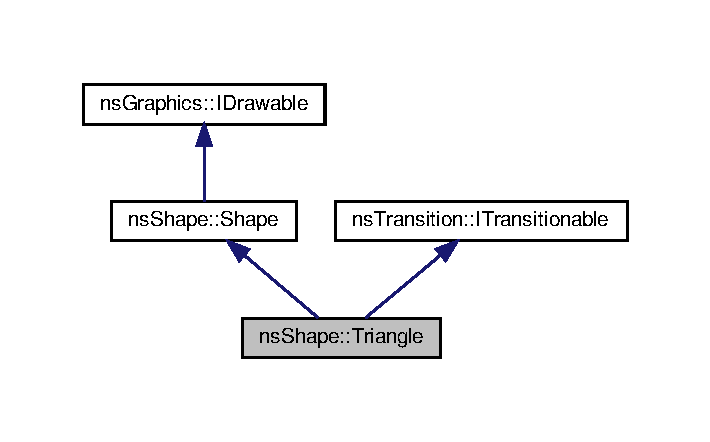
\includegraphics[width=341pt]{classns_shape_1_1_triangle__inherit__graph}
\end{center}
\end{figure}


Collaboration diagram for ns\+Shape\+:\+:Triangle\+:
\nopagebreak
\begin{figure}[H]
\begin{center}
\leavevmode
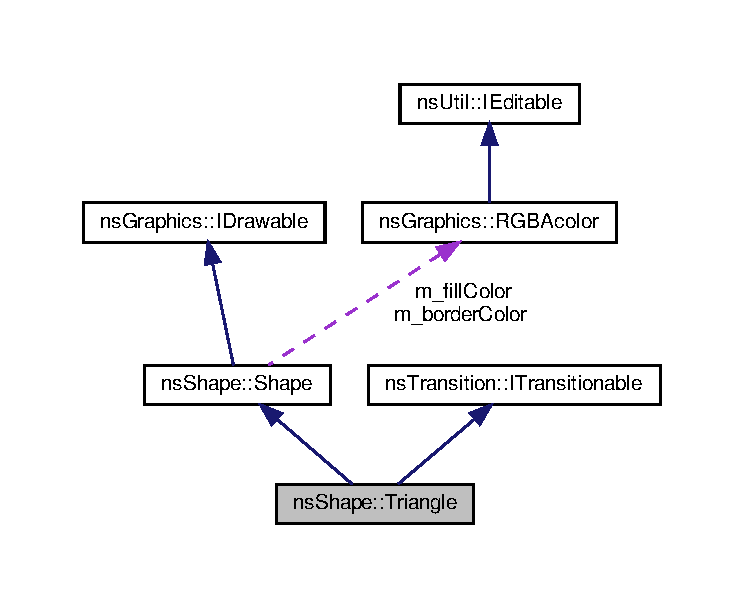
\includegraphics[width=350pt]{classns_shape_1_1_triangle__coll__graph}
\end{center}
\end{figure}
\subsection*{Public Types}
\begin{DoxyCompactItemize}
\item 
enum \hyperlink{classns_shape_1_1_triangle_adef21dd21ed3b5e4aa378f264abbe758}{Transition\+Ids} \{ \newline
\hyperlink{classns_shape_1_1_triangle_adef21dd21ed3b5e4aa378f264abbe758a9f20afd121f616d684ec0bd6b31dab54}{T\+R\+A\+N\+S\+I\+T\+I\+O\+N\+\_\+\+F\+I\+L\+L\+\_\+\+C\+O\+L\+O\+R\+\_\+\+R\+GB}, 
\hyperlink{classns_shape_1_1_triangle_adef21dd21ed3b5e4aa378f264abbe758a62867e3ea6657dbc0f9cc61bdca87be8}{T\+R\+A\+N\+S\+I\+T\+I\+O\+N\+\_\+\+F\+I\+L\+L\+\_\+\+C\+O\+L\+O\+R\+\_\+\+A\+L\+P\+HA}, 
\hyperlink{classns_shape_1_1_triangle_adef21dd21ed3b5e4aa378f264abbe758a43cba48c71b5804af47f7e1d5e1ecc9a}{T\+R\+A\+N\+S\+I\+T\+I\+O\+N\+\_\+\+B\+O\+R\+D\+E\+R\+\_\+\+C\+O\+L\+O\+R\+\_\+\+R\+GB}, 
\hyperlink{classns_shape_1_1_triangle_adef21dd21ed3b5e4aa378f264abbe758a541ff20fa337c2bfaaf7b29fbce4f586}{T\+R\+A\+N\+S\+I\+T\+I\+O\+N\+\_\+\+B\+O\+R\+D\+E\+R\+\_\+\+C\+O\+L\+O\+R\+\_\+\+A\+L\+P\+HA}, 
\newline
\hyperlink{classns_shape_1_1_triangle_adef21dd21ed3b5e4aa378f264abbe758aba96bb1e08665d081bedc72f56a85976}{T\+R\+A\+N\+S\+I\+T\+I\+O\+N\+\_\+\+F\+I\+R\+S\+T\+\_\+\+P\+O\+S\+I\+T\+I\+ON}, 
\hyperlink{classns_shape_1_1_triangle_adef21dd21ed3b5e4aa378f264abbe758a183e546c687567c28475575d67a12562}{T\+R\+A\+N\+S\+I\+T\+I\+O\+N\+\_\+\+S\+E\+C\+O\+N\+D\+\_\+\+P\+O\+S\+I\+T\+I\+ON}, 
\hyperlink{classns_shape_1_1_triangle_adef21dd21ed3b5e4aa378f264abbe758a634481d887d4cd8f6d5349d795c930cc}{T\+R\+A\+N\+S\+I\+T\+I\+O\+N\+\_\+\+T\+H\+I\+R\+D\+\_\+\+P\+O\+S\+I\+T\+I\+ON}
 \}\begin{DoxyCompactList}\small\item\em Transition\+Ids \+: Liste de toutes les transitions que cet élément peut exécuter. \end{DoxyCompactList}
\end{DoxyCompactItemize}
\subsection*{Public Member Functions}
\begin{DoxyCompactItemize}
\item 
\hyperlink{classns_shape_1_1_triangle_a72e60fed26e09d01757828ec019134c7}{Triangle} (const \hyperlink{classns_graphics_1_1_vec2_d}{ns\+Graphics\+::\+Vec2D} \&first\+Position, const \hyperlink{classns_graphics_1_1_vec2_d}{ns\+Graphics\+::\+Vec2D} \&second\+Position, const \hyperlink{classns_graphics_1_1_vec2_d}{ns\+Graphics\+::\+Vec2D} \&third\+Position, const \hyperlink{classns_graphics_1_1_r_g_b_acolor}{ns\+Graphics\+::\+R\+G\+B\+Acolor} \&fill\+Color, const \hyperlink{classns_graphics_1_1_r_g_b_acolor}{ns\+Graphics\+::\+R\+G\+B\+Acolor} \&border\+Color=\hyperlink{namespacens_graphics_ab2001ad03cceb2565849e04465618c1e}{ns\+Graphics\+::\+K\+Transparent})
\begin{DoxyCompactList}\small\item\em Constructeur pour la classe \hyperlink{classns_shape_1_1_triangle}{Triangle}. \end{DoxyCompactList}\item 
virtual \hyperlink{classns_shape_1_1_triangle_ae59fd091a1005d0e4a7e648487c69739}{$\sim$\+Triangle} () override=default
\begin{DoxyCompactList}\small\item\em Destructeur virtuel pour la classe \hyperlink{classns_shape_1_1_triangle}{Triangle}. \end{DoxyCompactList}\item 
virtual void \hyperlink{classns_shape_1_1_triangle_a4b3867fb0e15995b2a6c261d9b0d968d}{draw} (\hyperlink{class_min_g_l}{Min\+GL} \&window) const override
\begin{DoxyCompactList}\small\item\em Fonction pour afficher l\textquotesingle{}objet. \end{DoxyCompactList}\item 
virtual void \hyperlink{classns_shape_1_1_triangle_a745ce53bf673b56a23a30f732a041834}{get\+Values} (const int \&id, std\+::vector$<$ float $>$ \&values) override
\begin{DoxyCompactList}\small\item\em Récupère des valeurs dans un vecteur de float pour l\textquotesingle{}ID spécifié \end{DoxyCompactList}\item 
virtual void \hyperlink{classns_shape_1_1_triangle_af1c6cb0d5d12d8df0bd66c46ec793b22}{set\+Values} (const int \&id, const std\+::vector$<$ float $>$ \&values) override
\begin{DoxyCompactList}\small\item\em Définit les nouvelles valeurs pour l\textquotesingle{}ID spécifié \end{DoxyCompactList}\item 
\hyperlink{classns_shape_1_1_triangle}{Triangle} \hyperlink{classns_shape_1_1_triangle_a828914e234103dd5efece0030bd6ea12}{operator+} (const \hyperlink{classns_graphics_1_1_vec2_d}{ns\+Graphics\+::\+Vec2D} \&position) const
\begin{DoxyCompactList}\small\item\em Opérateur de décalage. \end{DoxyCompactList}\item 
\hyperlink{classns_shape_1_1_triangle}{Triangle} \hyperlink{classns_shape_1_1_triangle_adf2b03fb750f4269ed8ebfd25b5cb665}{operator$\ast$} (const float \&f) const
\begin{DoxyCompactList}\small\item\em Opérateur de réduction. \end{DoxyCompactList}\item 
const \hyperlink{classns_graphics_1_1_vec2_d}{ns\+Graphics\+::\+Vec2D} \& \hyperlink{classns_shape_1_1_triangle_ad82e289ac4c9fd8cc569b7a79771fc5f}{get\+First\+Position} () const
\begin{DoxyCompactList}\small\item\em Récupère la position du premier sommet du triangle. \end{DoxyCompactList}\item 
void \hyperlink{classns_shape_1_1_triangle_a9cbdb05c4f337961adccadf1aec48b1b}{set\+First\+Position} (const \hyperlink{classns_graphics_1_1_vec2_d}{ns\+Graphics\+::\+Vec2D} \&first\+Position)
\begin{DoxyCompactList}\small\item\em Définit la nouvelle position du premier sommet du triangle. \end{DoxyCompactList}\item 
const \hyperlink{classns_graphics_1_1_vec2_d}{ns\+Graphics\+::\+Vec2D} \& \hyperlink{classns_shape_1_1_triangle_a0222c889721e15942fde8719727da6ef}{get\+Second\+Position} () const
\begin{DoxyCompactList}\small\item\em Récupère la position du second sommet du triangle. \end{DoxyCompactList}\item 
void \hyperlink{classns_shape_1_1_triangle_a18f911ec00c99e29eec695a49c2e051e}{set\+Second\+Position} (const \hyperlink{classns_graphics_1_1_vec2_d}{ns\+Graphics\+::\+Vec2D} \&second\+Position)
\begin{DoxyCompactList}\small\item\em Définit la nouvelle position du second sommet du triangle. \end{DoxyCompactList}\item 
const \hyperlink{classns_graphics_1_1_vec2_d}{ns\+Graphics\+::\+Vec2D} \& \hyperlink{classns_shape_1_1_triangle_a8ff04f062cf1dcb119f9e814ce8f943a}{get\+Third\+Position} () const
\begin{DoxyCompactList}\small\item\em Récupère la position du troisième sommet du triangle. \end{DoxyCompactList}\item 
void \hyperlink{classns_shape_1_1_triangle_a7af3264cac9e8333ec5d7315bc931047}{set\+Third\+Position} (const \hyperlink{classns_graphics_1_1_vec2_d}{ns\+Graphics\+::\+Vec2D} \&third\+Position)
\begin{DoxyCompactList}\small\item\em Définit la nouvelle position du troisième sommet du triangle. \end{DoxyCompactList}\end{DoxyCompactItemize}
\subsection*{Additional Inherited Members}


\subsection{Detailed Description}
Classe représentant un triangle. 

Definition at line 25 of file triangle.\+h.



\subsection{Member Enumeration Documentation}
\mbox{\Hypertarget{classns_shape_1_1_triangle_adef21dd21ed3b5e4aa378f264abbe758}\label{classns_shape_1_1_triangle_adef21dd21ed3b5e4aa378f264abbe758}} 
\index{ns\+Shape\+::\+Triangle@{ns\+Shape\+::\+Triangle}!Transition\+Ids@{Transition\+Ids}}
\index{Transition\+Ids@{Transition\+Ids}!ns\+Shape\+::\+Triangle@{ns\+Shape\+::\+Triangle}}
\subsubsection{\texorpdfstring{Transition\+Ids}{TransitionIds}}
{\footnotesize\ttfamily enum \hyperlink{classns_shape_1_1_triangle_adef21dd21ed3b5e4aa378f264abbe758}{ns\+Shape\+::\+Triangle\+::\+Transition\+Ids}}



Transition\+Ids \+: Liste de toutes les transitions que cet élément peut exécuter. 

\begin{DoxyEnumFields}{Enumerator}
\raisebox{\heightof{T}}[0pt][0pt]{\index{T\+R\+A\+N\+S\+I\+T\+I\+O\+N\+\_\+\+F\+I\+L\+L\+\_\+\+C\+O\+L\+O\+R\+\_\+\+R\+GB@{T\+R\+A\+N\+S\+I\+T\+I\+O\+N\+\_\+\+F\+I\+L\+L\+\_\+\+C\+O\+L\+O\+R\+\_\+\+R\+GB}!ns\+Shape\+::\+Triangle@{ns\+Shape\+::\+Triangle}}\index{ns\+Shape\+::\+Triangle@{ns\+Shape\+::\+Triangle}!T\+R\+A\+N\+S\+I\+T\+I\+O\+N\+\_\+\+F\+I\+L\+L\+\_\+\+C\+O\+L\+O\+R\+\_\+\+R\+GB@{T\+R\+A\+N\+S\+I\+T\+I\+O\+N\+\_\+\+F\+I\+L\+L\+\_\+\+C\+O\+L\+O\+R\+\_\+\+R\+GB}}}\mbox{\Hypertarget{classns_shape_1_1_triangle_adef21dd21ed3b5e4aa378f264abbe758a9f20afd121f616d684ec0bd6b31dab54}\label{classns_shape_1_1_triangle_adef21dd21ed3b5e4aa378f264abbe758a9f20afd121f616d684ec0bd6b31dab54}} 
T\+R\+A\+N\+S\+I\+T\+I\+O\+N\+\_\+\+F\+I\+L\+L\+\_\+\+C\+O\+L\+O\+R\+\_\+\+R\+GB&Transition pour la couleur de remplissage \\
\hline

\raisebox{\heightof{T}}[0pt][0pt]{\index{T\+R\+A\+N\+S\+I\+T\+I\+O\+N\+\_\+\+F\+I\+L\+L\+\_\+\+C\+O\+L\+O\+R\+\_\+\+A\+L\+P\+HA@{T\+R\+A\+N\+S\+I\+T\+I\+O\+N\+\_\+\+F\+I\+L\+L\+\_\+\+C\+O\+L\+O\+R\+\_\+\+A\+L\+P\+HA}!ns\+Shape\+::\+Triangle@{ns\+Shape\+::\+Triangle}}\index{ns\+Shape\+::\+Triangle@{ns\+Shape\+::\+Triangle}!T\+R\+A\+N\+S\+I\+T\+I\+O\+N\+\_\+\+F\+I\+L\+L\+\_\+\+C\+O\+L\+O\+R\+\_\+\+A\+L\+P\+HA@{T\+R\+A\+N\+S\+I\+T\+I\+O\+N\+\_\+\+F\+I\+L\+L\+\_\+\+C\+O\+L\+O\+R\+\_\+\+A\+L\+P\+HA}}}\mbox{\Hypertarget{classns_shape_1_1_triangle_adef21dd21ed3b5e4aa378f264abbe758a62867e3ea6657dbc0f9cc61bdca87be8}\label{classns_shape_1_1_triangle_adef21dd21ed3b5e4aa378f264abbe758a62867e3ea6657dbc0f9cc61bdca87be8}} 
T\+R\+A\+N\+S\+I\+T\+I\+O\+N\+\_\+\+F\+I\+L\+L\+\_\+\+C\+O\+L\+O\+R\+\_\+\+A\+L\+P\+HA&Transition pour la transparence de remplissage \\
\hline

\raisebox{\heightof{T}}[0pt][0pt]{\index{T\+R\+A\+N\+S\+I\+T\+I\+O\+N\+\_\+\+B\+O\+R\+D\+E\+R\+\_\+\+C\+O\+L\+O\+R\+\_\+\+R\+GB@{T\+R\+A\+N\+S\+I\+T\+I\+O\+N\+\_\+\+B\+O\+R\+D\+E\+R\+\_\+\+C\+O\+L\+O\+R\+\_\+\+R\+GB}!ns\+Shape\+::\+Triangle@{ns\+Shape\+::\+Triangle}}\index{ns\+Shape\+::\+Triangle@{ns\+Shape\+::\+Triangle}!T\+R\+A\+N\+S\+I\+T\+I\+O\+N\+\_\+\+B\+O\+R\+D\+E\+R\+\_\+\+C\+O\+L\+O\+R\+\_\+\+R\+GB@{T\+R\+A\+N\+S\+I\+T\+I\+O\+N\+\_\+\+B\+O\+R\+D\+E\+R\+\_\+\+C\+O\+L\+O\+R\+\_\+\+R\+GB}}}\mbox{\Hypertarget{classns_shape_1_1_triangle_adef21dd21ed3b5e4aa378f264abbe758a43cba48c71b5804af47f7e1d5e1ecc9a}\label{classns_shape_1_1_triangle_adef21dd21ed3b5e4aa378f264abbe758a43cba48c71b5804af47f7e1d5e1ecc9a}} 
T\+R\+A\+N\+S\+I\+T\+I\+O\+N\+\_\+\+B\+O\+R\+D\+E\+R\+\_\+\+C\+O\+L\+O\+R\+\_\+\+R\+GB&Transition pour la couleur de bord \\
\hline

\raisebox{\heightof{T}}[0pt][0pt]{\index{T\+R\+A\+N\+S\+I\+T\+I\+O\+N\+\_\+\+B\+O\+R\+D\+E\+R\+\_\+\+C\+O\+L\+O\+R\+\_\+\+A\+L\+P\+HA@{T\+R\+A\+N\+S\+I\+T\+I\+O\+N\+\_\+\+B\+O\+R\+D\+E\+R\+\_\+\+C\+O\+L\+O\+R\+\_\+\+A\+L\+P\+HA}!ns\+Shape\+::\+Triangle@{ns\+Shape\+::\+Triangle}}\index{ns\+Shape\+::\+Triangle@{ns\+Shape\+::\+Triangle}!T\+R\+A\+N\+S\+I\+T\+I\+O\+N\+\_\+\+B\+O\+R\+D\+E\+R\+\_\+\+C\+O\+L\+O\+R\+\_\+\+A\+L\+P\+HA@{T\+R\+A\+N\+S\+I\+T\+I\+O\+N\+\_\+\+B\+O\+R\+D\+E\+R\+\_\+\+C\+O\+L\+O\+R\+\_\+\+A\+L\+P\+HA}}}\mbox{\Hypertarget{classns_shape_1_1_triangle_adef21dd21ed3b5e4aa378f264abbe758a541ff20fa337c2bfaaf7b29fbce4f586}\label{classns_shape_1_1_triangle_adef21dd21ed3b5e4aa378f264abbe758a541ff20fa337c2bfaaf7b29fbce4f586}} 
T\+R\+A\+N\+S\+I\+T\+I\+O\+N\+\_\+\+B\+O\+R\+D\+E\+R\+\_\+\+C\+O\+L\+O\+R\+\_\+\+A\+L\+P\+HA&Transition pour la transparence de bord \\
\hline

\raisebox{\heightof{T}}[0pt][0pt]{\index{T\+R\+A\+N\+S\+I\+T\+I\+O\+N\+\_\+\+F\+I\+R\+S\+T\+\_\+\+P\+O\+S\+I\+T\+I\+ON@{T\+R\+A\+N\+S\+I\+T\+I\+O\+N\+\_\+\+F\+I\+R\+S\+T\+\_\+\+P\+O\+S\+I\+T\+I\+ON}!ns\+Shape\+::\+Triangle@{ns\+Shape\+::\+Triangle}}\index{ns\+Shape\+::\+Triangle@{ns\+Shape\+::\+Triangle}!T\+R\+A\+N\+S\+I\+T\+I\+O\+N\+\_\+\+F\+I\+R\+S\+T\+\_\+\+P\+O\+S\+I\+T\+I\+ON@{T\+R\+A\+N\+S\+I\+T\+I\+O\+N\+\_\+\+F\+I\+R\+S\+T\+\_\+\+P\+O\+S\+I\+T\+I\+ON}}}\mbox{\Hypertarget{classns_shape_1_1_triangle_adef21dd21ed3b5e4aa378f264abbe758aba96bb1e08665d081bedc72f56a85976}\label{classns_shape_1_1_triangle_adef21dd21ed3b5e4aa378f264abbe758aba96bb1e08665d081bedc72f56a85976}} 
T\+R\+A\+N\+S\+I\+T\+I\+O\+N\+\_\+\+F\+I\+R\+S\+T\+\_\+\+P\+O\+S\+I\+T\+I\+ON&Transition pour la position du premier sommet \\
\hline

\raisebox{\heightof{T}}[0pt][0pt]{\index{T\+R\+A\+N\+S\+I\+T\+I\+O\+N\+\_\+\+S\+E\+C\+O\+N\+D\+\_\+\+P\+O\+S\+I\+T\+I\+ON@{T\+R\+A\+N\+S\+I\+T\+I\+O\+N\+\_\+\+S\+E\+C\+O\+N\+D\+\_\+\+P\+O\+S\+I\+T\+I\+ON}!ns\+Shape\+::\+Triangle@{ns\+Shape\+::\+Triangle}}\index{ns\+Shape\+::\+Triangle@{ns\+Shape\+::\+Triangle}!T\+R\+A\+N\+S\+I\+T\+I\+O\+N\+\_\+\+S\+E\+C\+O\+N\+D\+\_\+\+P\+O\+S\+I\+T\+I\+ON@{T\+R\+A\+N\+S\+I\+T\+I\+O\+N\+\_\+\+S\+E\+C\+O\+N\+D\+\_\+\+P\+O\+S\+I\+T\+I\+ON}}}\mbox{\Hypertarget{classns_shape_1_1_triangle_adef21dd21ed3b5e4aa378f264abbe758a183e546c687567c28475575d67a12562}\label{classns_shape_1_1_triangle_adef21dd21ed3b5e4aa378f264abbe758a183e546c687567c28475575d67a12562}} 
T\+R\+A\+N\+S\+I\+T\+I\+O\+N\+\_\+\+S\+E\+C\+O\+N\+D\+\_\+\+P\+O\+S\+I\+T\+I\+ON&Transition pour la position du second sommet \\
\hline

\raisebox{\heightof{T}}[0pt][0pt]{\index{T\+R\+A\+N\+S\+I\+T\+I\+O\+N\+\_\+\+T\+H\+I\+R\+D\+\_\+\+P\+O\+S\+I\+T\+I\+ON@{T\+R\+A\+N\+S\+I\+T\+I\+O\+N\+\_\+\+T\+H\+I\+R\+D\+\_\+\+P\+O\+S\+I\+T\+I\+ON}!ns\+Shape\+::\+Triangle@{ns\+Shape\+::\+Triangle}}\index{ns\+Shape\+::\+Triangle@{ns\+Shape\+::\+Triangle}!T\+R\+A\+N\+S\+I\+T\+I\+O\+N\+\_\+\+T\+H\+I\+R\+D\+\_\+\+P\+O\+S\+I\+T\+I\+ON@{T\+R\+A\+N\+S\+I\+T\+I\+O\+N\+\_\+\+T\+H\+I\+R\+D\+\_\+\+P\+O\+S\+I\+T\+I\+ON}}}\mbox{\Hypertarget{classns_shape_1_1_triangle_adef21dd21ed3b5e4aa378f264abbe758a634481d887d4cd8f6d5349d795c930cc}\label{classns_shape_1_1_triangle_adef21dd21ed3b5e4aa378f264abbe758a634481d887d4cd8f6d5349d795c930cc}} 
T\+R\+A\+N\+S\+I\+T\+I\+O\+N\+\_\+\+T\+H\+I\+R\+D\+\_\+\+P\+O\+S\+I\+T\+I\+ON&Transition pour la position du troisième sommet \\
\hline

\end{DoxyEnumFields}


Definition at line 32 of file triangle.\+h.



\subsection{Constructor \& Destructor Documentation}
\mbox{\Hypertarget{classns_shape_1_1_triangle_a72e60fed26e09d01757828ec019134c7}\label{classns_shape_1_1_triangle_a72e60fed26e09d01757828ec019134c7}} 
\index{ns\+Shape\+::\+Triangle@{ns\+Shape\+::\+Triangle}!Triangle@{Triangle}}
\index{Triangle@{Triangle}!ns\+Shape\+::\+Triangle@{ns\+Shape\+::\+Triangle}}
\subsubsection{\texorpdfstring{Triangle()}{Triangle()}}
{\footnotesize\ttfamily ns\+Shape\+::\+Triangle\+::\+Triangle (\begin{DoxyParamCaption}\item[{const \hyperlink{classns_graphics_1_1_vec2_d}{ns\+Graphics\+::\+Vec2D} \&}]{first\+Position,  }\item[{const \hyperlink{classns_graphics_1_1_vec2_d}{ns\+Graphics\+::\+Vec2D} \&}]{second\+Position,  }\item[{const \hyperlink{classns_graphics_1_1_vec2_d}{ns\+Graphics\+::\+Vec2D} \&}]{third\+Position,  }\item[{const \hyperlink{classns_graphics_1_1_r_g_b_acolor}{ns\+Graphics\+::\+R\+G\+B\+Acolor} \&}]{fill\+Color,  }\item[{const \hyperlink{classns_graphics_1_1_r_g_b_acolor}{ns\+Graphics\+::\+R\+G\+B\+Acolor} \&}]{border\+Color = {\ttfamily \hyperlink{namespacens_graphics_ab2001ad03cceb2565849e04465618c1e}{ns\+Graphics\+::\+K\+Transparent}} }\end{DoxyParamCaption})}



Constructeur pour la classe \hyperlink{classns_shape_1_1_triangle}{Triangle}. 


\begin{DoxyParams}[1]{Parameters}
\mbox{\tt in}  & {\em first\+Position} & \+: Position du premier sommet \\
\hline
\mbox{\tt in}  & {\em second\+Position} & \+: Position du second sommet \\
\hline
\mbox{\tt in}  & {\em third\+Position} & \+: Position du troisième sommet \\
\hline
\mbox{\tt in}  & {\em fill\+Color} & \+: Couleur de remplissage \\
\hline
\mbox{\tt in}  & {\em border\+Color} & \+: Couleur de bord \\
\hline
\end{DoxyParams}
\mbox{\Hypertarget{classns_shape_1_1_triangle_ae59fd091a1005d0e4a7e648487c69739}\label{classns_shape_1_1_triangle_ae59fd091a1005d0e4a7e648487c69739}} 
\index{ns\+Shape\+::\+Triangle@{ns\+Shape\+::\+Triangle}!````~Triangle@{$\sim$\+Triangle}}
\index{````~Triangle@{$\sim$\+Triangle}!ns\+Shape\+::\+Triangle@{ns\+Shape\+::\+Triangle}}
\subsubsection{\texorpdfstring{$\sim$\+Triangle()}{~Triangle()}}
{\footnotesize\ttfamily ns\+Shape\+::\+Triangle\+::$\sim$\+Triangle (\begin{DoxyParamCaption}{ }\end{DoxyParamCaption})\hspace{0.3cm}{\ttfamily [override]}, {\ttfamily [virtual]}, {\ttfamily [default]}}



Destructeur virtuel pour la classe \hyperlink{classns_shape_1_1_triangle}{Triangle}. 



\subsection{Member Function Documentation}
\mbox{\Hypertarget{classns_shape_1_1_triangle_a4b3867fb0e15995b2a6c261d9b0d968d}\label{classns_shape_1_1_triangle_a4b3867fb0e15995b2a6c261d9b0d968d}} 
\index{ns\+Shape\+::\+Triangle@{ns\+Shape\+::\+Triangle}!draw@{draw}}
\index{draw@{draw}!ns\+Shape\+::\+Triangle@{ns\+Shape\+::\+Triangle}}
\subsubsection{\texorpdfstring{draw()}{draw()}}
{\footnotesize\ttfamily virtual void ns\+Shape\+::\+Triangle\+::draw (\begin{DoxyParamCaption}\item[{\hyperlink{class_min_g_l}{Min\+GL} \&}]{window }\end{DoxyParamCaption}) const\hspace{0.3cm}{\ttfamily [override]}, {\ttfamily [virtual]}}



Fonction pour afficher l\textquotesingle{}objet. 



Implements \hyperlink{classns_graphics_1_1_i_drawable_abed8a61e1d507d31e76f0891f3bf9c51}{ns\+Graphics\+::\+I\+Drawable}.

\mbox{\Hypertarget{classns_shape_1_1_triangle_ad82e289ac4c9fd8cc569b7a79771fc5f}\label{classns_shape_1_1_triangle_ad82e289ac4c9fd8cc569b7a79771fc5f}} 
\index{ns\+Shape\+::\+Triangle@{ns\+Shape\+::\+Triangle}!get\+First\+Position@{get\+First\+Position}}
\index{get\+First\+Position@{get\+First\+Position}!ns\+Shape\+::\+Triangle@{ns\+Shape\+::\+Triangle}}
\subsubsection{\texorpdfstring{get\+First\+Position()}{getFirstPosition()}}
{\footnotesize\ttfamily const \hyperlink{classns_graphics_1_1_vec2_d}{ns\+Graphics\+::\+Vec2D} \& ns\+Shape\+::\+Triangle\+::get\+First\+Position (\begin{DoxyParamCaption}{ }\end{DoxyParamCaption}) const}



Récupère la position du premier sommet du triangle. 

\mbox{\Hypertarget{classns_shape_1_1_triangle_a0222c889721e15942fde8719727da6ef}\label{classns_shape_1_1_triangle_a0222c889721e15942fde8719727da6ef}} 
\index{ns\+Shape\+::\+Triangle@{ns\+Shape\+::\+Triangle}!get\+Second\+Position@{get\+Second\+Position}}
\index{get\+Second\+Position@{get\+Second\+Position}!ns\+Shape\+::\+Triangle@{ns\+Shape\+::\+Triangle}}
\subsubsection{\texorpdfstring{get\+Second\+Position()}{getSecondPosition()}}
{\footnotesize\ttfamily const \hyperlink{classns_graphics_1_1_vec2_d}{ns\+Graphics\+::\+Vec2D} \& ns\+Shape\+::\+Triangle\+::get\+Second\+Position (\begin{DoxyParamCaption}{ }\end{DoxyParamCaption}) const}



Récupère la position du second sommet du triangle. 

\mbox{\Hypertarget{classns_shape_1_1_triangle_a8ff04f062cf1dcb119f9e814ce8f943a}\label{classns_shape_1_1_triangle_a8ff04f062cf1dcb119f9e814ce8f943a}} 
\index{ns\+Shape\+::\+Triangle@{ns\+Shape\+::\+Triangle}!get\+Third\+Position@{get\+Third\+Position}}
\index{get\+Third\+Position@{get\+Third\+Position}!ns\+Shape\+::\+Triangle@{ns\+Shape\+::\+Triangle}}
\subsubsection{\texorpdfstring{get\+Third\+Position()}{getThirdPosition()}}
{\footnotesize\ttfamily const \hyperlink{classns_graphics_1_1_vec2_d}{ns\+Graphics\+::\+Vec2D} \& ns\+Shape\+::\+Triangle\+::get\+Third\+Position (\begin{DoxyParamCaption}{ }\end{DoxyParamCaption}) const}



Récupère la position du troisième sommet du triangle. 

\mbox{\Hypertarget{classns_shape_1_1_triangle_a745ce53bf673b56a23a30f732a041834}\label{classns_shape_1_1_triangle_a745ce53bf673b56a23a30f732a041834}} 
\index{ns\+Shape\+::\+Triangle@{ns\+Shape\+::\+Triangle}!get\+Values@{get\+Values}}
\index{get\+Values@{get\+Values}!ns\+Shape\+::\+Triangle@{ns\+Shape\+::\+Triangle}}
\subsubsection{\texorpdfstring{get\+Values()}{getValues()}}
{\footnotesize\ttfamily virtual void ns\+Shape\+::\+Triangle\+::get\+Values (\begin{DoxyParamCaption}\item[{const int \&}]{id,  }\item[{std\+::vector$<$ float $>$ \&}]{values }\end{DoxyParamCaption})\hspace{0.3cm}{\ttfamily [override]}, {\ttfamily [virtual]}}



Récupère des valeurs dans un vecteur de float pour l\textquotesingle{}ID spécifié 


\begin{DoxyParams}[1]{Parameters}
\mbox{\tt in}  & {\em id} & ID des valeurs a récupérer \\
\hline
\mbox{\tt in,out}  & {\em values} & Vecteur de valeurs a peupler \\
\hline
\end{DoxyParams}


Implements \hyperlink{classns_transition_1_1_i_transitionable_a5871a16fd47c1e5c8bacdd5da8597ed9}{ns\+Transition\+::\+I\+Transitionable}.

\mbox{\Hypertarget{classns_shape_1_1_triangle_adf2b03fb750f4269ed8ebfd25b5cb665}\label{classns_shape_1_1_triangle_adf2b03fb750f4269ed8ebfd25b5cb665}} 
\index{ns\+Shape\+::\+Triangle@{ns\+Shape\+::\+Triangle}!operator$\ast$@{operator$\ast$}}
\index{operator$\ast$@{operator$\ast$}!ns\+Shape\+::\+Triangle@{ns\+Shape\+::\+Triangle}}
\subsubsection{\texorpdfstring{operator$\ast$()}{operator*()}}
{\footnotesize\ttfamily \hyperlink{classns_shape_1_1_triangle}{Triangle} ns\+Shape\+::\+Triangle\+::operator$\ast$ (\begin{DoxyParamCaption}\item[{const float \&}]{f }\end{DoxyParamCaption}) const}



Opérateur de réduction. 


\begin{DoxyParams}[1]{Parameters}
\mbox{\tt in}  & {\em f} & \+: Nombre avec lequel multiplier la position actuelle \\
\hline
\end{DoxyParams}
\mbox{\Hypertarget{classns_shape_1_1_triangle_a828914e234103dd5efece0030bd6ea12}\label{classns_shape_1_1_triangle_a828914e234103dd5efece0030bd6ea12}} 
\index{ns\+Shape\+::\+Triangle@{ns\+Shape\+::\+Triangle}!operator+@{operator+}}
\index{operator+@{operator+}!ns\+Shape\+::\+Triangle@{ns\+Shape\+::\+Triangle}}
\subsubsection{\texorpdfstring{operator+()}{operator+()}}
{\footnotesize\ttfamily \hyperlink{classns_shape_1_1_triangle}{Triangle} ns\+Shape\+::\+Triangle\+::operator+ (\begin{DoxyParamCaption}\item[{const \hyperlink{classns_graphics_1_1_vec2_d}{ns\+Graphics\+::\+Vec2D} \&}]{position }\end{DoxyParamCaption}) const}



Opérateur de décalage. 


\begin{DoxyParams}[1]{Parameters}
\mbox{\tt in}  & {\em position} & \+: Position a additionner \\
\hline
\end{DoxyParams}
\mbox{\Hypertarget{classns_shape_1_1_triangle_a9cbdb05c4f337961adccadf1aec48b1b}\label{classns_shape_1_1_triangle_a9cbdb05c4f337961adccadf1aec48b1b}} 
\index{ns\+Shape\+::\+Triangle@{ns\+Shape\+::\+Triangle}!set\+First\+Position@{set\+First\+Position}}
\index{set\+First\+Position@{set\+First\+Position}!ns\+Shape\+::\+Triangle@{ns\+Shape\+::\+Triangle}}
\subsubsection{\texorpdfstring{set\+First\+Position()}{setFirstPosition()}}
{\footnotesize\ttfamily void ns\+Shape\+::\+Triangle\+::set\+First\+Position (\begin{DoxyParamCaption}\item[{const \hyperlink{classns_graphics_1_1_vec2_d}{ns\+Graphics\+::\+Vec2D} \&}]{first\+Position }\end{DoxyParamCaption})}



Définit la nouvelle position du premier sommet du triangle. 


\begin{DoxyParams}[1]{Parameters}
\mbox{\tt in}  & {\em first\+Position} & \+: Nouvelle position du premier sommet \\
\hline
\end{DoxyParams}
\mbox{\Hypertarget{classns_shape_1_1_triangle_a18f911ec00c99e29eec695a49c2e051e}\label{classns_shape_1_1_triangle_a18f911ec00c99e29eec695a49c2e051e}} 
\index{ns\+Shape\+::\+Triangle@{ns\+Shape\+::\+Triangle}!set\+Second\+Position@{set\+Second\+Position}}
\index{set\+Second\+Position@{set\+Second\+Position}!ns\+Shape\+::\+Triangle@{ns\+Shape\+::\+Triangle}}
\subsubsection{\texorpdfstring{set\+Second\+Position()}{setSecondPosition()}}
{\footnotesize\ttfamily void ns\+Shape\+::\+Triangle\+::set\+Second\+Position (\begin{DoxyParamCaption}\item[{const \hyperlink{classns_graphics_1_1_vec2_d}{ns\+Graphics\+::\+Vec2D} \&}]{second\+Position }\end{DoxyParamCaption})}



Définit la nouvelle position du second sommet du triangle. 


\begin{DoxyParams}[1]{Parameters}
\mbox{\tt in}  & {\em second\+Position} & \+: Nouvelle position du second sommet \\
\hline
\end{DoxyParams}
\mbox{\Hypertarget{classns_shape_1_1_triangle_a7af3264cac9e8333ec5d7315bc931047}\label{classns_shape_1_1_triangle_a7af3264cac9e8333ec5d7315bc931047}} 
\index{ns\+Shape\+::\+Triangle@{ns\+Shape\+::\+Triangle}!set\+Third\+Position@{set\+Third\+Position}}
\index{set\+Third\+Position@{set\+Third\+Position}!ns\+Shape\+::\+Triangle@{ns\+Shape\+::\+Triangle}}
\subsubsection{\texorpdfstring{set\+Third\+Position()}{setThirdPosition()}}
{\footnotesize\ttfamily void ns\+Shape\+::\+Triangle\+::set\+Third\+Position (\begin{DoxyParamCaption}\item[{const \hyperlink{classns_graphics_1_1_vec2_d}{ns\+Graphics\+::\+Vec2D} \&}]{third\+Position }\end{DoxyParamCaption})}



Définit la nouvelle position du troisième sommet du triangle. 


\begin{DoxyParams}[1]{Parameters}
\mbox{\tt in}  & {\em third\+Position} & \+: Nouvelle position du troisième sommet \\
\hline
\end{DoxyParams}
\mbox{\Hypertarget{classns_shape_1_1_triangle_af1c6cb0d5d12d8df0bd66c46ec793b22}\label{classns_shape_1_1_triangle_af1c6cb0d5d12d8df0bd66c46ec793b22}} 
\index{ns\+Shape\+::\+Triangle@{ns\+Shape\+::\+Triangle}!set\+Values@{set\+Values}}
\index{set\+Values@{set\+Values}!ns\+Shape\+::\+Triangle@{ns\+Shape\+::\+Triangle}}
\subsubsection{\texorpdfstring{set\+Values()}{setValues()}}
{\footnotesize\ttfamily virtual void ns\+Shape\+::\+Triangle\+::set\+Values (\begin{DoxyParamCaption}\item[{const int \&}]{id,  }\item[{const std\+::vector$<$ float $>$ \&}]{values }\end{DoxyParamCaption})\hspace{0.3cm}{\ttfamily [override]}, {\ttfamily [virtual]}}



Définit les nouvelles valeurs pour l\textquotesingle{}ID spécifié 


\begin{DoxyParams}[1]{Parameters}
\mbox{\tt in}  & {\em id} & ID des valeurs a définir \\
\hline
\mbox{\tt in}  & {\em values} & Vecteur des nouvelles valeurs a appliquer \\
\hline
\end{DoxyParams}


Implements \hyperlink{classns_transition_1_1_i_transitionable_ade37d29f7f2ca4890ed0e2e64d033197}{ns\+Transition\+::\+I\+Transitionable}.



The documentation for this class was generated from the following file\+:\begin{DoxyCompactItemize}
\item 
libs/mingl/shape/\hyperlink{triangle_8h}{triangle.\+h}\end{DoxyCompactItemize}

\hypertarget{classns_graphics_1_1_vec2_d}{}\section{ns\+Graphics\+:\+:Vec2D Class Reference}
\label{classns_graphics_1_1_vec2_d}\index{ns\+Graphics\+::\+Vec2D@{ns\+Graphics\+::\+Vec2D}}


Classe représentant un vecteur deux-\/dimensionnel.  




{\ttfamily \#include $<$vec2d.\+h$>$}



Inheritance diagram for ns\+Graphics\+:\+:Vec2D\+:
\nopagebreak
\begin{figure}[H]
\begin{center}
\leavevmode
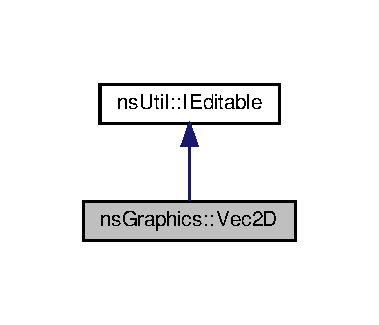
\includegraphics[width=182pt]{classns_graphics_1_1_vec2_d__inherit__graph}
\end{center}
\end{figure}


Collaboration diagram for ns\+Graphics\+:\+:Vec2D\+:
\nopagebreak
\begin{figure}[H]
\begin{center}
\leavevmode
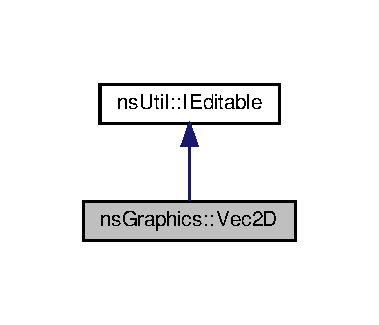
\includegraphics[width=182pt]{classns_graphics_1_1_vec2_d__coll__graph}
\end{center}
\end{figure}
\subsection*{Public Member Functions}
\begin{DoxyCompactItemize}
\item 
\hyperlink{classns_graphics_1_1_vec2_d_a4a2fdd532ded3c29b7a3bd6e5a23fadf}{Vec2D} (const int \&x=0, const int \&y=0)
\begin{DoxyCompactList}\small\item\em Constructeur pour la classe \hyperlink{classns_graphics_1_1_vec2_d}{Vec2D}. \end{DoxyCompactList}\item 
\hyperlink{classns_graphics_1_1_vec2_d_ae409c698404abced934b589d58513767}{Vec2D} (const \hyperlink{classns_graphics_1_1_vec2_d}{Vec2D} \&pos)
\begin{DoxyCompactList}\small\item\em Constructeur de recopie pour la classe \hyperlink{classns_graphics_1_1_vec2_d}{Vec2D}. \end{DoxyCompactList}\item 
\hyperlink{classns_graphics_1_1_vec2_d}{Vec2D} \hyperlink{classns_graphics_1_1_vec2_d_aded521aea98ae5b1fdd19f4f9e2df74a}{operator+} () const
\begin{DoxyCompactList}\small\item\em Opérateur unaire plus. \end{DoxyCompactList}\item 
\hyperlink{classns_graphics_1_1_vec2_d}{Vec2D} \hyperlink{classns_graphics_1_1_vec2_d_a3cc10af3b04df2c6bf85460ced5c63a7}{operator-\/} () const
\begin{DoxyCompactList}\small\item\em Opérateur unaire moins. \end{DoxyCompactList}\item 
\hyperlink{classns_graphics_1_1_vec2_d}{Vec2D} \hyperlink{classns_graphics_1_1_vec2_d_a59d565535347c6d0974be9a2333a5806}{operator+} (const \hyperlink{classns_graphics_1_1_vec2_d}{Vec2D} \&pos) const
\begin{DoxyCompactList}\small\item\em Opérateur d\textquotesingle{}addition. \end{DoxyCompactList}\item 
\hyperlink{classns_graphics_1_1_vec2_d}{Vec2D} \hyperlink{classns_graphics_1_1_vec2_d_a6431bcd5dd86fbaf119bed9cf01a13f2}{operator-\/} (const \hyperlink{classns_graphics_1_1_vec2_d}{Vec2D} \&pos) const
\begin{DoxyCompactList}\small\item\em Opérateur de soustraction. \end{DoxyCompactList}\item 
\hyperlink{classns_graphics_1_1_vec2_d}{Vec2D} \hyperlink{classns_graphics_1_1_vec2_d_afed7035dfbafeffbfac737fb39d4fb90}{operator$\ast$} (const \hyperlink{classns_graphics_1_1_vec2_d}{Vec2D} \&pos) const
\begin{DoxyCompactList}\small\item\em Opérateur de multiplication. \end{DoxyCompactList}\item 
\hyperlink{classns_graphics_1_1_vec2_d}{Vec2D} \hyperlink{classns_graphics_1_1_vec2_d_a7eb4139a171785d5f2f337cee77b9fb0}{operator$\ast$} (const float \&n) const
\begin{DoxyCompactList}\small\item\em Opérateur de multiplication. \end{DoxyCompactList}\item 
\hyperlink{classns_graphics_1_1_vec2_d}{Vec2D} \hyperlink{classns_graphics_1_1_vec2_d_aaabc44f047e46433d0115fbc49b3ae2f}{operator/} (const \hyperlink{classns_graphics_1_1_vec2_d}{Vec2D} \&pos) const
\begin{DoxyCompactList}\small\item\em Opérateur de division. \end{DoxyCompactList}\item 
\hyperlink{classns_graphics_1_1_vec2_d}{Vec2D} \hyperlink{classns_graphics_1_1_vec2_d_ae3adeb741fa6137acf0edbcf02ca58af}{operator/} (const float \&n) const
\begin{DoxyCompactList}\small\item\em Opérateur de division. \end{DoxyCompactList}\item 
\hyperlink{classns_graphics_1_1_vec2_d}{Vec2D} \hyperlink{classns_graphics_1_1_vec2_d_a43281403abbad9948eacca4d37fc61dc}{operator\%} (const \hyperlink{classns_graphics_1_1_vec2_d}{Vec2D} \&pos) const
\begin{DoxyCompactList}\small\item\em Opérateur modulo. \end{DoxyCompactList}\item 
bool \hyperlink{classns_graphics_1_1_vec2_d_a94b4b8420a450dd284311c49cb0b2e6b}{operator==} (const \hyperlink{classns_graphics_1_1_vec2_d}{Vec2D} \&pos) const
\begin{DoxyCompactList}\small\item\em Opérateur d\textquotesingle{}égalité \end{DoxyCompactList}\item 
bool \hyperlink{classns_graphics_1_1_vec2_d_affaed949190e8cb5a3c8f9813b31eb0d}{operator!=} (const \hyperlink{classns_graphics_1_1_vec2_d}{Vec2D} \&pos) const
\begin{DoxyCompactList}\small\item\em Opérateur d\textquotesingle{}inégalité \end{DoxyCompactList}\item 
bool \hyperlink{classns_graphics_1_1_vec2_d_accfe96cfa5b8495a0b14c7087068064e}{operator$<$} (const \hyperlink{classns_graphics_1_1_vec2_d}{Vec2D} \&pos) const
\begin{DoxyCompactList}\small\item\em Opérateur de stricte infériorité (Vérifie la stricte infériorité de la magnitude des deux vecteurs) \end{DoxyCompactList}\item 
bool \hyperlink{classns_graphics_1_1_vec2_d_a30da0e7984d8c3e7a66bbdcdcc24c9cb}{operator$>$} (const \hyperlink{classns_graphics_1_1_vec2_d}{Vec2D} \&pos) const
\begin{DoxyCompactList}\small\item\em Opérateur de stricte supériorité (Vérifie la stricte supériorité de la magnitude des deux vecteurs) \end{DoxyCompactList}\item 
bool \hyperlink{classns_graphics_1_1_vec2_d_afd5e0e3ba77ef971f8d022d69a4a2647}{operator$<$=} (const \hyperlink{classns_graphics_1_1_vec2_d}{Vec2D} \&pos) const
\begin{DoxyCompactList}\small\item\em Opérateur d\textquotesingle{}infériorité (Vérifie l\textquotesingle{}infériorité de la magnitude des deux vecteurs) \end{DoxyCompactList}\item 
bool \hyperlink{classns_graphics_1_1_vec2_d_a478dad2852611070874c6c9e5663b570}{operator$>$=} (const \hyperlink{classns_graphics_1_1_vec2_d}{Vec2D} \&pos) const
\begin{DoxyCompactList}\small\item\em Opérateur de supériorité (Vérifie la supériorité de la magnitude des deux vecteurs) \end{DoxyCompactList}\item 
\hyperlink{classns_graphics_1_1_vec2_d}{Vec2D} \& \hyperlink{classns_graphics_1_1_vec2_d_a041926192c1d2c579b12dcf1eb1725d5}{operator=} (const \hyperlink{classns_graphics_1_1_vec2_d}{Vec2D} \&pos)
\begin{DoxyCompactList}\small\item\em Opérateur d\textquotesingle{}assignement. \end{DoxyCompactList}\item 
\hyperlink{classns_graphics_1_1_vec2_d}{Vec2D} \& \hyperlink{classns_graphics_1_1_vec2_d_aafd8b68f1cb9dcfcf92a96714e58c5ec}{operator+=} (const \hyperlink{classns_graphics_1_1_vec2_d}{Vec2D} \&pos)
\begin{DoxyCompactList}\small\item\em Opérateur d\textquotesingle{}addition avec assignement. \end{DoxyCompactList}\item 
\hyperlink{classns_graphics_1_1_vec2_d}{Vec2D} \& \hyperlink{classns_graphics_1_1_vec2_d_aa9b0986206c35bb5c0043db02548fce4}{operator-\/=} (const \hyperlink{classns_graphics_1_1_vec2_d}{Vec2D} \&pos)
\begin{DoxyCompactList}\small\item\em Opérateur de soustraction avec assignement. \end{DoxyCompactList}\item 
\hyperlink{classns_graphics_1_1_vec2_d}{Vec2D} \& \hyperlink{classns_graphics_1_1_vec2_d_a6e0e661361c0f3081fa2d9488978771e}{operator$\ast$=} (const \hyperlink{classns_graphics_1_1_vec2_d}{Vec2D} \&pos)
\begin{DoxyCompactList}\small\item\em Opérateur de multiplication avec assignement. \end{DoxyCompactList}\item 
\hyperlink{classns_graphics_1_1_vec2_d}{Vec2D} \& \hyperlink{classns_graphics_1_1_vec2_d_a1146ac9d05c667bb4a46140858953711}{operator/=} (const \hyperlink{classns_graphics_1_1_vec2_d}{Vec2D} \&pos)
\begin{DoxyCompactList}\small\item\em Opérateur de division avec assignement. \end{DoxyCompactList}\item 
\hyperlink{classns_graphics_1_1_vec2_d}{Vec2D} \& \hyperlink{classns_graphics_1_1_vec2_d_a57003f3d4660f986c3c21c027ac8b154}{operator\%=} (const \hyperlink{classns_graphics_1_1_vec2_d}{Vec2D} \&pos)
\begin{DoxyCompactList}\small\item\em Opérateur modulo avec assignement. \end{DoxyCompactList}\item 
bool \hyperlink{classns_graphics_1_1_vec2_d_aa02cee45c2d8aa2d9b7e08dfb6c1dfca}{is\+Colliding} (\hyperlink{classns_graphics_1_1_vec2_d}{Vec2D} first\+Corner, \hyperlink{classns_graphics_1_1_vec2_d}{Vec2D} second\+Corner) const
\begin{DoxyCompactList}\small\item\em Retourne vrai si le vecteur actuel est compris entre deux vecteurs formant un rectangle. \end{DoxyCompactList}\item 
double \hyperlink{classns_graphics_1_1_vec2_d_adf603dcb6f44ff82f3d48df141e11fe7}{compute\+Magnitude} () const
\begin{DoxyCompactList}\small\item\em Calcule la magnitude de ce vecteur. \end{DoxyCompactList}\item 
int \hyperlink{classns_graphics_1_1_vec2_d_abcf3d729b05b3cd93e9eff21c74b89a1}{getX} () const
\begin{DoxyCompactList}\small\item\em Récupère la position X (abscisse) \end{DoxyCompactList}\item 
void \hyperlink{classns_graphics_1_1_vec2_d_ae9d371fdd3817c6e9a3a1ae6ed3fd17d}{setX} (int x)
\begin{DoxyCompactList}\small\item\em Définit la nouvelle position X (abscisse) \end{DoxyCompactList}\item 
int \hyperlink{classns_graphics_1_1_vec2_d_ae70fbda9cca27b9dc0fe068a38ae5e5e}{getY} () const
\begin{DoxyCompactList}\small\item\em Récupère la position Y (ordonnée) \end{DoxyCompactList}\item 
void \hyperlink{classns_graphics_1_1_vec2_d_ac0e752e399ab2f727fe2644540b1208f}{setY} (int y)
\begin{DoxyCompactList}\small\item\em Définit la nouvelle position Y (ordonnée) \end{DoxyCompactList}\end{DoxyCompactItemize}
\subsection*{Static Public Member Functions}
\begin{DoxyCompactItemize}
\item 
static \hyperlink{classns_graphics_1_1_vec2_d}{Vec2D} \hyperlink{classns_graphics_1_1_vec2_d_a8a4760c6a33beb77d1e7a850b44129fc}{min} (const \hyperlink{classns_graphics_1_1_vec2_d}{Vec2D} \&p1, const \hyperlink{classns_graphics_1_1_vec2_d}{Vec2D} \&p2)
\begin{DoxyCompactList}\small\item\em Retourne le vecteur le plus petit entre les deux passés en argument. \end{DoxyCompactList}\item 
static bool \hyperlink{classns_graphics_1_1_vec2_d_a77c8619c34dcb2e7b5d9337da0fcfe59}{minf} (const \hyperlink{classns_graphics_1_1_vec2_d}{Vec2D} \&p1, const \hyperlink{classns_graphics_1_1_vec2_d}{Vec2D} \&p2)
\begin{DoxyCompactList}\small\item\em Retourne vrai si le premier vecteur est le plus petit des deux. \end{DoxyCompactList}\end{DoxyCompactItemize}
\subsection*{Protected Member Functions}
\begin{DoxyCompactItemize}
\item 
virtual std\+::ostream \& \hyperlink{classns_graphics_1_1_vec2_d_ac271e47658195475bfe8b39f163dcebd}{\+\_\+\+Edit} (std\+::ostream \&os=std\+::cout) const override
\begin{DoxyCompactList}\small\item\em Fonction appelée pour injecter l\textquotesingle{}objet courant dans un flux. \end{DoxyCompactList}\end{DoxyCompactItemize}


\subsection{Detailed Description}
Classe représentant un vecteur deux-\/dimensionnel. 

Definition at line 25 of file vec2d.\+h.



\subsection{Constructor \& Destructor Documentation}
\mbox{\Hypertarget{classns_graphics_1_1_vec2_d_a4a2fdd532ded3c29b7a3bd6e5a23fadf}\label{classns_graphics_1_1_vec2_d_a4a2fdd532ded3c29b7a3bd6e5a23fadf}} 
\index{ns\+Graphics\+::\+Vec2D@{ns\+Graphics\+::\+Vec2D}!Vec2D@{Vec2D}}
\index{Vec2D@{Vec2D}!ns\+Graphics\+::\+Vec2D@{ns\+Graphics\+::\+Vec2D}}
\subsubsection{\texorpdfstring{Vec2\+D()}{Vec2D()}\hspace{0.1cm}{\footnotesize\ttfamily [1/2]}}
{\footnotesize\ttfamily ns\+Graphics\+::\+Vec2\+D\+::\+Vec2D (\begin{DoxyParamCaption}\item[{const int \&}]{x = {\ttfamily 0},  }\item[{const int \&}]{y = {\ttfamily 0} }\end{DoxyParamCaption})}



Constructeur pour la classe \hyperlink{classns_graphics_1_1_vec2_d}{Vec2D}. 


\begin{DoxyParams}[1]{Parameters}
\mbox{\tt in}  & {\em x} & \+: Position X (abscisse) du vecteur \\
\hline
\mbox{\tt in}  & {\em y} & \+: Position Y (ordonnée) du vecteur \\
\hline
\end{DoxyParams}
\mbox{\Hypertarget{classns_graphics_1_1_vec2_d_ae409c698404abced934b589d58513767}\label{classns_graphics_1_1_vec2_d_ae409c698404abced934b589d58513767}} 
\index{ns\+Graphics\+::\+Vec2D@{ns\+Graphics\+::\+Vec2D}!Vec2D@{Vec2D}}
\index{Vec2D@{Vec2D}!ns\+Graphics\+::\+Vec2D@{ns\+Graphics\+::\+Vec2D}}
\subsubsection{\texorpdfstring{Vec2\+D()}{Vec2D()}\hspace{0.1cm}{\footnotesize\ttfamily [2/2]}}
{\footnotesize\ttfamily ns\+Graphics\+::\+Vec2\+D\+::\+Vec2D (\begin{DoxyParamCaption}\item[{const \hyperlink{classns_graphics_1_1_vec2_d}{Vec2D} \&}]{pos }\end{DoxyParamCaption})}



Constructeur de recopie pour la classe \hyperlink{classns_graphics_1_1_vec2_d}{Vec2D}. 


\begin{DoxyParams}[1]{Parameters}
\mbox{\tt in}  & {\em pos} & \+: \hyperlink{classns_graphics_1_1_vec2_d}{Vec2D} a copier \\
\hline
\end{DoxyParams}


\subsection{Member Function Documentation}
\mbox{\Hypertarget{classns_graphics_1_1_vec2_d_ac271e47658195475bfe8b39f163dcebd}\label{classns_graphics_1_1_vec2_d_ac271e47658195475bfe8b39f163dcebd}} 
\index{ns\+Graphics\+::\+Vec2D@{ns\+Graphics\+::\+Vec2D}!\+\_\+\+Edit@{\+\_\+\+Edit}}
\index{\+\_\+\+Edit@{\+\_\+\+Edit}!ns\+Graphics\+::\+Vec2D@{ns\+Graphics\+::\+Vec2D}}
\subsubsection{\texorpdfstring{\+\_\+\+Edit()}{\_Edit()}}
{\footnotesize\ttfamily virtual std\+::ostream\& ns\+Graphics\+::\+Vec2\+D\+::\+\_\+\+Edit (\begin{DoxyParamCaption}\item[{std\+::ostream \&}]{os = {\ttfamily std\+:\+:cout} }\end{DoxyParamCaption}) const\hspace{0.3cm}{\ttfamily [override]}, {\ttfamily [protected]}, {\ttfamily [virtual]}}



Fonction appelée pour injecter l\textquotesingle{}objet courant dans un flux. 


\begin{DoxyParams}[1]{Parameters}
\mbox{\tt in}  & {\em os} & \+: Flux dans lequel injecter \\
\hline
\end{DoxyParams}


Implements \hyperlink{classns_util_1_1_i_editable_ab20bbe582b95383ed3f1453109035853}{ns\+Util\+::\+I\+Editable}.

\mbox{\Hypertarget{classns_graphics_1_1_vec2_d_adf603dcb6f44ff82f3d48df141e11fe7}\label{classns_graphics_1_1_vec2_d_adf603dcb6f44ff82f3d48df141e11fe7}} 
\index{ns\+Graphics\+::\+Vec2D@{ns\+Graphics\+::\+Vec2D}!compute\+Magnitude@{compute\+Magnitude}}
\index{compute\+Magnitude@{compute\+Magnitude}!ns\+Graphics\+::\+Vec2D@{ns\+Graphics\+::\+Vec2D}}
\subsubsection{\texorpdfstring{compute\+Magnitude()}{computeMagnitude()}}
{\footnotesize\ttfamily double ns\+Graphics\+::\+Vec2\+D\+::compute\+Magnitude (\begin{DoxyParamCaption}{ }\end{DoxyParamCaption}) const}



Calcule la magnitude de ce vecteur. 

\begin{DoxyReturn}{Returns}
Magnitude du vecteur 
\end{DoxyReturn}
\mbox{\Hypertarget{classns_graphics_1_1_vec2_d_abcf3d729b05b3cd93e9eff21c74b89a1}\label{classns_graphics_1_1_vec2_d_abcf3d729b05b3cd93e9eff21c74b89a1}} 
\index{ns\+Graphics\+::\+Vec2D@{ns\+Graphics\+::\+Vec2D}!getX@{getX}}
\index{getX@{getX}!ns\+Graphics\+::\+Vec2D@{ns\+Graphics\+::\+Vec2D}}
\subsubsection{\texorpdfstring{get\+X()}{getX()}}
{\footnotesize\ttfamily int ns\+Graphics\+::\+Vec2\+D\+::getX (\begin{DoxyParamCaption}{ }\end{DoxyParamCaption}) const}



Récupère la position X (abscisse) 

\begin{DoxyReturn}{Returns}
Une référence constante vers m\+\_\+x 
\end{DoxyReturn}
\mbox{\Hypertarget{classns_graphics_1_1_vec2_d_ae70fbda9cca27b9dc0fe068a38ae5e5e}\label{classns_graphics_1_1_vec2_d_ae70fbda9cca27b9dc0fe068a38ae5e5e}} 
\index{ns\+Graphics\+::\+Vec2D@{ns\+Graphics\+::\+Vec2D}!getY@{getY}}
\index{getY@{getY}!ns\+Graphics\+::\+Vec2D@{ns\+Graphics\+::\+Vec2D}}
\subsubsection{\texorpdfstring{get\+Y()}{getY()}}
{\footnotesize\ttfamily int ns\+Graphics\+::\+Vec2\+D\+::getY (\begin{DoxyParamCaption}{ }\end{DoxyParamCaption}) const}



Récupère la position Y (ordonnée) 

\begin{DoxyReturn}{Returns}
Une référence constante vers m\+\_\+y 
\end{DoxyReturn}
\mbox{\Hypertarget{classns_graphics_1_1_vec2_d_aa02cee45c2d8aa2d9b7e08dfb6c1dfca}\label{classns_graphics_1_1_vec2_d_aa02cee45c2d8aa2d9b7e08dfb6c1dfca}} 
\index{ns\+Graphics\+::\+Vec2D@{ns\+Graphics\+::\+Vec2D}!is\+Colliding@{is\+Colliding}}
\index{is\+Colliding@{is\+Colliding}!ns\+Graphics\+::\+Vec2D@{ns\+Graphics\+::\+Vec2D}}
\subsubsection{\texorpdfstring{is\+Colliding()}{isColliding()}}
{\footnotesize\ttfamily bool ns\+Graphics\+::\+Vec2\+D\+::is\+Colliding (\begin{DoxyParamCaption}\item[{\hyperlink{classns_graphics_1_1_vec2_d}{Vec2D}}]{first\+Corner,  }\item[{\hyperlink{classns_graphics_1_1_vec2_d}{Vec2D}}]{second\+Corner }\end{DoxyParamCaption}) const}



Retourne vrai si le vecteur actuel est compris entre deux vecteurs formant un rectangle. 


\begin{DoxyParams}[1]{Parameters}
\mbox{\tt in}  & {\em first\+Corner} & \+: Premier vecteur \\
\hline
\mbox{\tt in}  & {\em second\+Corner} & \+: Second vecteur \\
\hline
\end{DoxyParams}
\mbox{\Hypertarget{classns_graphics_1_1_vec2_d_a8a4760c6a33beb77d1e7a850b44129fc}\label{classns_graphics_1_1_vec2_d_a8a4760c6a33beb77d1e7a850b44129fc}} 
\index{ns\+Graphics\+::\+Vec2D@{ns\+Graphics\+::\+Vec2D}!min@{min}}
\index{min@{min}!ns\+Graphics\+::\+Vec2D@{ns\+Graphics\+::\+Vec2D}}
\subsubsection{\texorpdfstring{min()}{min()}}
{\footnotesize\ttfamily static \hyperlink{classns_graphics_1_1_vec2_d}{Vec2D} ns\+Graphics\+::\+Vec2\+D\+::min (\begin{DoxyParamCaption}\item[{const \hyperlink{classns_graphics_1_1_vec2_d}{Vec2D} \&}]{p1,  }\item[{const \hyperlink{classns_graphics_1_1_vec2_d}{Vec2D} \&}]{p2 }\end{DoxyParamCaption})\hspace{0.3cm}{\ttfamily [static]}}



Retourne le vecteur le plus petit entre les deux passés en argument. 


\begin{DoxyParams}[1]{Parameters}
\mbox{\tt in}  & {\em p1} & \+: Premier vecteur \\
\hline
\mbox{\tt in}  & {\em p2} & \+: Second vecteur \\
\hline
\end{DoxyParams}
\mbox{\Hypertarget{classns_graphics_1_1_vec2_d_a77c8619c34dcb2e7b5d9337da0fcfe59}\label{classns_graphics_1_1_vec2_d_a77c8619c34dcb2e7b5d9337da0fcfe59}} 
\index{ns\+Graphics\+::\+Vec2D@{ns\+Graphics\+::\+Vec2D}!minf@{minf}}
\index{minf@{minf}!ns\+Graphics\+::\+Vec2D@{ns\+Graphics\+::\+Vec2D}}
\subsubsection{\texorpdfstring{minf()}{minf()}}
{\footnotesize\ttfamily static bool ns\+Graphics\+::\+Vec2\+D\+::minf (\begin{DoxyParamCaption}\item[{const \hyperlink{classns_graphics_1_1_vec2_d}{Vec2D} \&}]{p1,  }\item[{const \hyperlink{classns_graphics_1_1_vec2_d}{Vec2D} \&}]{p2 }\end{DoxyParamCaption})\hspace{0.3cm}{\ttfamily [static]}}



Retourne vrai si le premier vecteur est le plus petit des deux. 


\begin{DoxyParams}[1]{Parameters}
\mbox{\tt in}  & {\em p1} & \+: Premier vecteur \\
\hline
\mbox{\tt in}  & {\em p2} & \+: Second vecteur \\
\hline
\end{DoxyParams}
\mbox{\Hypertarget{classns_graphics_1_1_vec2_d_affaed949190e8cb5a3c8f9813b31eb0d}\label{classns_graphics_1_1_vec2_d_affaed949190e8cb5a3c8f9813b31eb0d}} 
\index{ns\+Graphics\+::\+Vec2D@{ns\+Graphics\+::\+Vec2D}!operator"!=@{operator"!=}}
\index{operator"!=@{operator"!=}!ns\+Graphics\+::\+Vec2D@{ns\+Graphics\+::\+Vec2D}}
\subsubsection{\texorpdfstring{operator"!=()}{operator!=()}}
{\footnotesize\ttfamily bool ns\+Graphics\+::\+Vec2\+D\+::operator!= (\begin{DoxyParamCaption}\item[{const \hyperlink{classns_graphics_1_1_vec2_d}{Vec2D} \&}]{pos }\end{DoxyParamCaption}) const}



Opérateur d\textquotesingle{}inégalité 


\begin{DoxyParams}[1]{Parameters}
\mbox{\tt in}  & {\em pos} & \+: Vecteur avec lequel vérifier l\textquotesingle{}inégalité \\
\hline
\end{DoxyParams}
\mbox{\Hypertarget{classns_graphics_1_1_vec2_d_a43281403abbad9948eacca4d37fc61dc}\label{classns_graphics_1_1_vec2_d_a43281403abbad9948eacca4d37fc61dc}} 
\index{ns\+Graphics\+::\+Vec2D@{ns\+Graphics\+::\+Vec2D}!operator\%@{operator\%}}
\index{operator\%@{operator\%}!ns\+Graphics\+::\+Vec2D@{ns\+Graphics\+::\+Vec2D}}
\subsubsection{\texorpdfstring{operator\%()}{operator\%()}}
{\footnotesize\ttfamily \hyperlink{classns_graphics_1_1_vec2_d}{Vec2D} ns\+Graphics\+::\+Vec2\+D\+::operator\% (\begin{DoxyParamCaption}\item[{const \hyperlink{classns_graphics_1_1_vec2_d}{Vec2D} \&}]{pos }\end{DoxyParamCaption}) const}



Opérateur modulo. 


\begin{DoxyParams}[1]{Parameters}
\mbox{\tt in}  & {\em pos} & \+: Vecteur avec lequel faire un modulo \\
\hline
\end{DoxyParams}
\mbox{\Hypertarget{classns_graphics_1_1_vec2_d_a57003f3d4660f986c3c21c027ac8b154}\label{classns_graphics_1_1_vec2_d_a57003f3d4660f986c3c21c027ac8b154}} 
\index{ns\+Graphics\+::\+Vec2D@{ns\+Graphics\+::\+Vec2D}!operator\%=@{operator\%=}}
\index{operator\%=@{operator\%=}!ns\+Graphics\+::\+Vec2D@{ns\+Graphics\+::\+Vec2D}}
\subsubsection{\texorpdfstring{operator\%=()}{operator\%=()}}
{\footnotesize\ttfamily \hyperlink{classns_graphics_1_1_vec2_d}{Vec2D} \& ns\+Graphics\+::\+Vec2\+D\+::operator\%= (\begin{DoxyParamCaption}\item[{const \hyperlink{classns_graphics_1_1_vec2_d}{Vec2D} \&}]{pos }\end{DoxyParamCaption})}



Opérateur modulo avec assignement. 


\begin{DoxyParams}[1]{Parameters}
\mbox{\tt in}  & {\em pos} & \+: Vecteur avec lequel faire un modulo sur le vecteur actuel \\
\hline
\end{DoxyParams}
\mbox{\Hypertarget{classns_graphics_1_1_vec2_d_afed7035dfbafeffbfac737fb39d4fb90}\label{classns_graphics_1_1_vec2_d_afed7035dfbafeffbfac737fb39d4fb90}} 
\index{ns\+Graphics\+::\+Vec2D@{ns\+Graphics\+::\+Vec2D}!operator$\ast$@{operator$\ast$}}
\index{operator$\ast$@{operator$\ast$}!ns\+Graphics\+::\+Vec2D@{ns\+Graphics\+::\+Vec2D}}
\subsubsection{\texorpdfstring{operator$\ast$()}{operator*()}\hspace{0.1cm}{\footnotesize\ttfamily [1/2]}}
{\footnotesize\ttfamily \hyperlink{classns_graphics_1_1_vec2_d}{Vec2D} ns\+Graphics\+::\+Vec2\+D\+::operator$\ast$ (\begin{DoxyParamCaption}\item[{const \hyperlink{classns_graphics_1_1_vec2_d}{Vec2D} \&}]{pos }\end{DoxyParamCaption}) const}



Opérateur de multiplication. 


\begin{DoxyParams}[1]{Parameters}
\mbox{\tt in}  & {\em pos} & \+: Vecteur a multiplier \\
\hline
\end{DoxyParams}
\mbox{\Hypertarget{classns_graphics_1_1_vec2_d_a7eb4139a171785d5f2f337cee77b9fb0}\label{classns_graphics_1_1_vec2_d_a7eb4139a171785d5f2f337cee77b9fb0}} 
\index{ns\+Graphics\+::\+Vec2D@{ns\+Graphics\+::\+Vec2D}!operator$\ast$@{operator$\ast$}}
\index{operator$\ast$@{operator$\ast$}!ns\+Graphics\+::\+Vec2D@{ns\+Graphics\+::\+Vec2D}}
\subsubsection{\texorpdfstring{operator$\ast$()}{operator*()}\hspace{0.1cm}{\footnotesize\ttfamily [2/2]}}
{\footnotesize\ttfamily \hyperlink{classns_graphics_1_1_vec2_d}{Vec2D} ns\+Graphics\+::\+Vec2\+D\+::operator$\ast$ (\begin{DoxyParamCaption}\item[{const float \&}]{n }\end{DoxyParamCaption}) const}



Opérateur de multiplication. 


\begin{DoxyParams}[1]{Parameters}
\mbox{\tt in}  & {\em n} & \+: Nombre avec lequel multiplier le vecteur actuel \\
\hline
\end{DoxyParams}
\mbox{\Hypertarget{classns_graphics_1_1_vec2_d_a6e0e661361c0f3081fa2d9488978771e}\label{classns_graphics_1_1_vec2_d_a6e0e661361c0f3081fa2d9488978771e}} 
\index{ns\+Graphics\+::\+Vec2D@{ns\+Graphics\+::\+Vec2D}!operator$\ast$=@{operator$\ast$=}}
\index{operator$\ast$=@{operator$\ast$=}!ns\+Graphics\+::\+Vec2D@{ns\+Graphics\+::\+Vec2D}}
\subsubsection{\texorpdfstring{operator$\ast$=()}{operator*=()}}
{\footnotesize\ttfamily \hyperlink{classns_graphics_1_1_vec2_d}{Vec2D} \& ns\+Graphics\+::\+Vec2\+D\+::operator$\ast$= (\begin{DoxyParamCaption}\item[{const \hyperlink{classns_graphics_1_1_vec2_d}{Vec2D} \&}]{pos }\end{DoxyParamCaption})}



Opérateur de multiplication avec assignement. 


\begin{DoxyParams}[1]{Parameters}
\mbox{\tt in}  & {\em pos} & \+: Vecteur avec lequel multiplier le vecteur actuel \\
\hline
\end{DoxyParams}
\mbox{\Hypertarget{classns_graphics_1_1_vec2_d_aded521aea98ae5b1fdd19f4f9e2df74a}\label{classns_graphics_1_1_vec2_d_aded521aea98ae5b1fdd19f4f9e2df74a}} 
\index{ns\+Graphics\+::\+Vec2D@{ns\+Graphics\+::\+Vec2D}!operator+@{operator+}}
\index{operator+@{operator+}!ns\+Graphics\+::\+Vec2D@{ns\+Graphics\+::\+Vec2D}}
\subsubsection{\texorpdfstring{operator+()}{operator+()}\hspace{0.1cm}{\footnotesize\ttfamily [1/2]}}
{\footnotesize\ttfamily \hyperlink{classns_graphics_1_1_vec2_d}{Vec2D} ns\+Graphics\+::\+Vec2\+D\+::operator+ (\begin{DoxyParamCaption}{ }\end{DoxyParamCaption}) const}



Opérateur unaire plus. 

\mbox{\Hypertarget{classns_graphics_1_1_vec2_d_a59d565535347c6d0974be9a2333a5806}\label{classns_graphics_1_1_vec2_d_a59d565535347c6d0974be9a2333a5806}} 
\index{ns\+Graphics\+::\+Vec2D@{ns\+Graphics\+::\+Vec2D}!operator+@{operator+}}
\index{operator+@{operator+}!ns\+Graphics\+::\+Vec2D@{ns\+Graphics\+::\+Vec2D}}
\subsubsection{\texorpdfstring{operator+()}{operator+()}\hspace{0.1cm}{\footnotesize\ttfamily [2/2]}}
{\footnotesize\ttfamily \hyperlink{classns_graphics_1_1_vec2_d}{Vec2D} ns\+Graphics\+::\+Vec2\+D\+::operator+ (\begin{DoxyParamCaption}\item[{const \hyperlink{classns_graphics_1_1_vec2_d}{Vec2D} \&}]{pos }\end{DoxyParamCaption}) const}



Opérateur d\textquotesingle{}addition. 


\begin{DoxyParams}[1]{Parameters}
\mbox{\tt in}  & {\em pos} & \+: Vecteur a additionner \\
\hline
\end{DoxyParams}
\mbox{\Hypertarget{classns_graphics_1_1_vec2_d_aafd8b68f1cb9dcfcf92a96714e58c5ec}\label{classns_graphics_1_1_vec2_d_aafd8b68f1cb9dcfcf92a96714e58c5ec}} 
\index{ns\+Graphics\+::\+Vec2D@{ns\+Graphics\+::\+Vec2D}!operator+=@{operator+=}}
\index{operator+=@{operator+=}!ns\+Graphics\+::\+Vec2D@{ns\+Graphics\+::\+Vec2D}}
\subsubsection{\texorpdfstring{operator+=()}{operator+=()}}
{\footnotesize\ttfamily \hyperlink{classns_graphics_1_1_vec2_d}{Vec2D} \& ns\+Graphics\+::\+Vec2\+D\+::operator+= (\begin{DoxyParamCaption}\item[{const \hyperlink{classns_graphics_1_1_vec2_d}{Vec2D} \&}]{pos }\end{DoxyParamCaption})}



Opérateur d\textquotesingle{}addition avec assignement. 


\begin{DoxyParams}[1]{Parameters}
\mbox{\tt in}  & {\em pos} & \+: Vecteur avec lequel additionner le vecteur actuel \\
\hline
\end{DoxyParams}
\mbox{\Hypertarget{classns_graphics_1_1_vec2_d_a3cc10af3b04df2c6bf85460ced5c63a7}\label{classns_graphics_1_1_vec2_d_a3cc10af3b04df2c6bf85460ced5c63a7}} 
\index{ns\+Graphics\+::\+Vec2D@{ns\+Graphics\+::\+Vec2D}!operator-\/@{operator-\/}}
\index{operator-\/@{operator-\/}!ns\+Graphics\+::\+Vec2D@{ns\+Graphics\+::\+Vec2D}}
\subsubsection{\texorpdfstring{operator-\/()}{operator-()}\hspace{0.1cm}{\footnotesize\ttfamily [1/2]}}
{\footnotesize\ttfamily \hyperlink{classns_graphics_1_1_vec2_d}{Vec2D} ns\+Graphics\+::\+Vec2\+D\+::operator-\/ (\begin{DoxyParamCaption}{ }\end{DoxyParamCaption}) const}



Opérateur unaire moins. 

\mbox{\Hypertarget{classns_graphics_1_1_vec2_d_a6431bcd5dd86fbaf119bed9cf01a13f2}\label{classns_graphics_1_1_vec2_d_a6431bcd5dd86fbaf119bed9cf01a13f2}} 
\index{ns\+Graphics\+::\+Vec2D@{ns\+Graphics\+::\+Vec2D}!operator-\/@{operator-\/}}
\index{operator-\/@{operator-\/}!ns\+Graphics\+::\+Vec2D@{ns\+Graphics\+::\+Vec2D}}
\subsubsection{\texorpdfstring{operator-\/()}{operator-()}\hspace{0.1cm}{\footnotesize\ttfamily [2/2]}}
{\footnotesize\ttfamily \hyperlink{classns_graphics_1_1_vec2_d}{Vec2D} ns\+Graphics\+::\+Vec2\+D\+::operator-\/ (\begin{DoxyParamCaption}\item[{const \hyperlink{classns_graphics_1_1_vec2_d}{Vec2D} \&}]{pos }\end{DoxyParamCaption}) const}



Opérateur de soustraction. 


\begin{DoxyParams}[1]{Parameters}
\mbox{\tt in}  & {\em pos} & \+: Vecteur a soustraire \\
\hline
\end{DoxyParams}
\mbox{\Hypertarget{classns_graphics_1_1_vec2_d_aa9b0986206c35bb5c0043db02548fce4}\label{classns_graphics_1_1_vec2_d_aa9b0986206c35bb5c0043db02548fce4}} 
\index{ns\+Graphics\+::\+Vec2D@{ns\+Graphics\+::\+Vec2D}!operator-\/=@{operator-\/=}}
\index{operator-\/=@{operator-\/=}!ns\+Graphics\+::\+Vec2D@{ns\+Graphics\+::\+Vec2D}}
\subsubsection{\texorpdfstring{operator-\/=()}{operator-=()}}
{\footnotesize\ttfamily \hyperlink{classns_graphics_1_1_vec2_d}{Vec2D} \& ns\+Graphics\+::\+Vec2\+D\+::operator-\/= (\begin{DoxyParamCaption}\item[{const \hyperlink{classns_graphics_1_1_vec2_d}{Vec2D} \&}]{pos }\end{DoxyParamCaption})}



Opérateur de soustraction avec assignement. 


\begin{DoxyParams}[1]{Parameters}
\mbox{\tt in}  & {\em pos} & \+: Vecteur avec lequel soustraire le vecteur actuel \\
\hline
\end{DoxyParams}
\mbox{\Hypertarget{classns_graphics_1_1_vec2_d_aaabc44f047e46433d0115fbc49b3ae2f}\label{classns_graphics_1_1_vec2_d_aaabc44f047e46433d0115fbc49b3ae2f}} 
\index{ns\+Graphics\+::\+Vec2D@{ns\+Graphics\+::\+Vec2D}!operator/@{operator/}}
\index{operator/@{operator/}!ns\+Graphics\+::\+Vec2D@{ns\+Graphics\+::\+Vec2D}}
\subsubsection{\texorpdfstring{operator/()}{operator/()}\hspace{0.1cm}{\footnotesize\ttfamily [1/2]}}
{\footnotesize\ttfamily \hyperlink{classns_graphics_1_1_vec2_d}{Vec2D} ns\+Graphics\+::\+Vec2\+D\+::operator/ (\begin{DoxyParamCaption}\item[{const \hyperlink{classns_graphics_1_1_vec2_d}{Vec2D} \&}]{pos }\end{DoxyParamCaption}) const}



Opérateur de division. 


\begin{DoxyParams}[1]{Parameters}
\mbox{\tt in}  & {\em pos} & \+: Vecteur a diviser \\
\hline
\end{DoxyParams}
\mbox{\Hypertarget{classns_graphics_1_1_vec2_d_ae3adeb741fa6137acf0edbcf02ca58af}\label{classns_graphics_1_1_vec2_d_ae3adeb741fa6137acf0edbcf02ca58af}} 
\index{ns\+Graphics\+::\+Vec2D@{ns\+Graphics\+::\+Vec2D}!operator/@{operator/}}
\index{operator/@{operator/}!ns\+Graphics\+::\+Vec2D@{ns\+Graphics\+::\+Vec2D}}
\subsubsection{\texorpdfstring{operator/()}{operator/()}\hspace{0.1cm}{\footnotesize\ttfamily [2/2]}}
{\footnotesize\ttfamily \hyperlink{classns_graphics_1_1_vec2_d}{Vec2D} ns\+Graphics\+::\+Vec2\+D\+::operator/ (\begin{DoxyParamCaption}\item[{const float \&}]{n }\end{DoxyParamCaption}) const}



Opérateur de division. 


\begin{DoxyParams}[1]{Parameters}
\mbox{\tt in}  & {\em n} & \+: Nombre avec lequel diviser le vecteur actuel \\
\hline
\end{DoxyParams}
\mbox{\Hypertarget{classns_graphics_1_1_vec2_d_a1146ac9d05c667bb4a46140858953711}\label{classns_graphics_1_1_vec2_d_a1146ac9d05c667bb4a46140858953711}} 
\index{ns\+Graphics\+::\+Vec2D@{ns\+Graphics\+::\+Vec2D}!operator/=@{operator/=}}
\index{operator/=@{operator/=}!ns\+Graphics\+::\+Vec2D@{ns\+Graphics\+::\+Vec2D}}
\subsubsection{\texorpdfstring{operator/=()}{operator/=()}}
{\footnotesize\ttfamily \hyperlink{classns_graphics_1_1_vec2_d}{Vec2D} \& ns\+Graphics\+::\+Vec2\+D\+::operator/= (\begin{DoxyParamCaption}\item[{const \hyperlink{classns_graphics_1_1_vec2_d}{Vec2D} \&}]{pos }\end{DoxyParamCaption})}



Opérateur de division avec assignement. 


\begin{DoxyParams}[1]{Parameters}
\mbox{\tt in}  & {\em pos} & \+: Vecteur avec lequel diviser le vecteur actuel \\
\hline
\end{DoxyParams}
\mbox{\Hypertarget{classns_graphics_1_1_vec2_d_accfe96cfa5b8495a0b14c7087068064e}\label{classns_graphics_1_1_vec2_d_accfe96cfa5b8495a0b14c7087068064e}} 
\index{ns\+Graphics\+::\+Vec2D@{ns\+Graphics\+::\+Vec2D}!operator$<$@{operator$<$}}
\index{operator$<$@{operator$<$}!ns\+Graphics\+::\+Vec2D@{ns\+Graphics\+::\+Vec2D}}
\subsubsection{\texorpdfstring{operator$<$()}{operator<()}}
{\footnotesize\ttfamily bool ns\+Graphics\+::\+Vec2\+D\+::operator$<$ (\begin{DoxyParamCaption}\item[{const \hyperlink{classns_graphics_1_1_vec2_d}{Vec2D} \&}]{pos }\end{DoxyParamCaption}) const}



Opérateur de stricte infériorité (Vérifie la stricte infériorité de la magnitude des deux vecteurs) 


\begin{DoxyParams}[1]{Parameters}
\mbox{\tt in}  & {\em pos} & \+: Vecteur avec lequel vérifier la stricte infériorité \\
\hline
\end{DoxyParams}
\mbox{\Hypertarget{classns_graphics_1_1_vec2_d_afd5e0e3ba77ef971f8d022d69a4a2647}\label{classns_graphics_1_1_vec2_d_afd5e0e3ba77ef971f8d022d69a4a2647}} 
\index{ns\+Graphics\+::\+Vec2D@{ns\+Graphics\+::\+Vec2D}!operator$<$=@{operator$<$=}}
\index{operator$<$=@{operator$<$=}!ns\+Graphics\+::\+Vec2D@{ns\+Graphics\+::\+Vec2D}}
\subsubsection{\texorpdfstring{operator$<$=()}{operator<=()}}
{\footnotesize\ttfamily bool ns\+Graphics\+::\+Vec2\+D\+::operator$<$= (\begin{DoxyParamCaption}\item[{const \hyperlink{classns_graphics_1_1_vec2_d}{Vec2D} \&}]{pos }\end{DoxyParamCaption}) const}



Opérateur d\textquotesingle{}infériorité (Vérifie l\textquotesingle{}infériorité de la magnitude des deux vecteurs) 


\begin{DoxyParams}[1]{Parameters}
\mbox{\tt in}  & {\em pos} & \+: Vecteur avec lequel vérifier l\textquotesingle{}infériorité \\
\hline
\end{DoxyParams}
\mbox{\Hypertarget{classns_graphics_1_1_vec2_d_a041926192c1d2c579b12dcf1eb1725d5}\label{classns_graphics_1_1_vec2_d_a041926192c1d2c579b12dcf1eb1725d5}} 
\index{ns\+Graphics\+::\+Vec2D@{ns\+Graphics\+::\+Vec2D}!operator=@{operator=}}
\index{operator=@{operator=}!ns\+Graphics\+::\+Vec2D@{ns\+Graphics\+::\+Vec2D}}
\subsubsection{\texorpdfstring{operator=()}{operator=()}}
{\footnotesize\ttfamily \hyperlink{classns_graphics_1_1_vec2_d}{Vec2D} \& ns\+Graphics\+::\+Vec2\+D\+::operator= (\begin{DoxyParamCaption}\item[{const \hyperlink{classns_graphics_1_1_vec2_d}{Vec2D} \&}]{pos }\end{DoxyParamCaption})}



Opérateur d\textquotesingle{}assignement. 


\begin{DoxyParams}[1]{Parameters}
\mbox{\tt in}  & {\em pos} & \+: Vecteur source \\
\hline
\end{DoxyParams}
\mbox{\Hypertarget{classns_graphics_1_1_vec2_d_a94b4b8420a450dd284311c49cb0b2e6b}\label{classns_graphics_1_1_vec2_d_a94b4b8420a450dd284311c49cb0b2e6b}} 
\index{ns\+Graphics\+::\+Vec2D@{ns\+Graphics\+::\+Vec2D}!operator==@{operator==}}
\index{operator==@{operator==}!ns\+Graphics\+::\+Vec2D@{ns\+Graphics\+::\+Vec2D}}
\subsubsection{\texorpdfstring{operator==()}{operator==()}}
{\footnotesize\ttfamily bool ns\+Graphics\+::\+Vec2\+D\+::operator== (\begin{DoxyParamCaption}\item[{const \hyperlink{classns_graphics_1_1_vec2_d}{Vec2D} \&}]{pos }\end{DoxyParamCaption}) const}



Opérateur d\textquotesingle{}égalité 


\begin{DoxyParams}[1]{Parameters}
\mbox{\tt in}  & {\em pos} & \+: Vecteur avec lequel vérifier l\textquotesingle{}égalité \\
\hline
\end{DoxyParams}
\mbox{\Hypertarget{classns_graphics_1_1_vec2_d_a30da0e7984d8c3e7a66bbdcdcc24c9cb}\label{classns_graphics_1_1_vec2_d_a30da0e7984d8c3e7a66bbdcdcc24c9cb}} 
\index{ns\+Graphics\+::\+Vec2D@{ns\+Graphics\+::\+Vec2D}!operator$>$@{operator$>$}}
\index{operator$>$@{operator$>$}!ns\+Graphics\+::\+Vec2D@{ns\+Graphics\+::\+Vec2D}}
\subsubsection{\texorpdfstring{operator$>$()}{operator>()}}
{\footnotesize\ttfamily bool ns\+Graphics\+::\+Vec2\+D\+::operator$>$ (\begin{DoxyParamCaption}\item[{const \hyperlink{classns_graphics_1_1_vec2_d}{Vec2D} \&}]{pos }\end{DoxyParamCaption}) const}



Opérateur de stricte supériorité (Vérifie la stricte supériorité de la magnitude des deux vecteurs) 


\begin{DoxyParams}[1]{Parameters}
\mbox{\tt in}  & {\em pos} & \+: Vecteur avec lequel vérifier la stricte supériorité \\
\hline
\end{DoxyParams}
\mbox{\Hypertarget{classns_graphics_1_1_vec2_d_a478dad2852611070874c6c9e5663b570}\label{classns_graphics_1_1_vec2_d_a478dad2852611070874c6c9e5663b570}} 
\index{ns\+Graphics\+::\+Vec2D@{ns\+Graphics\+::\+Vec2D}!operator$>$=@{operator$>$=}}
\index{operator$>$=@{operator$>$=}!ns\+Graphics\+::\+Vec2D@{ns\+Graphics\+::\+Vec2D}}
\subsubsection{\texorpdfstring{operator$>$=()}{operator>=()}}
{\footnotesize\ttfamily bool ns\+Graphics\+::\+Vec2\+D\+::operator$>$= (\begin{DoxyParamCaption}\item[{const \hyperlink{classns_graphics_1_1_vec2_d}{Vec2D} \&}]{pos }\end{DoxyParamCaption}) const}



Opérateur de supériorité (Vérifie la supériorité de la magnitude des deux vecteurs) 


\begin{DoxyParams}[1]{Parameters}
\mbox{\tt in}  & {\em pos} & \+: Vecteur avec lequel vérifier la supériorité \\
\hline
\end{DoxyParams}
\mbox{\Hypertarget{classns_graphics_1_1_vec2_d_ae9d371fdd3817c6e9a3a1ae6ed3fd17d}\label{classns_graphics_1_1_vec2_d_ae9d371fdd3817c6e9a3a1ae6ed3fd17d}} 
\index{ns\+Graphics\+::\+Vec2D@{ns\+Graphics\+::\+Vec2D}!setX@{setX}}
\index{setX@{setX}!ns\+Graphics\+::\+Vec2D@{ns\+Graphics\+::\+Vec2D}}
\subsubsection{\texorpdfstring{set\+X()}{setX()}}
{\footnotesize\ttfamily void ns\+Graphics\+::\+Vec2\+D\+::setX (\begin{DoxyParamCaption}\item[{int}]{x }\end{DoxyParamCaption})}



Définit la nouvelle position X (abscisse) 


\begin{DoxyParams}[1]{Parameters}
\mbox{\tt in}  & {\em x} & \+: Nouvelle position X \\
\hline
\end{DoxyParams}
\mbox{\Hypertarget{classns_graphics_1_1_vec2_d_ac0e752e399ab2f727fe2644540b1208f}\label{classns_graphics_1_1_vec2_d_ac0e752e399ab2f727fe2644540b1208f}} 
\index{ns\+Graphics\+::\+Vec2D@{ns\+Graphics\+::\+Vec2D}!setY@{setY}}
\index{setY@{setY}!ns\+Graphics\+::\+Vec2D@{ns\+Graphics\+::\+Vec2D}}
\subsubsection{\texorpdfstring{set\+Y()}{setY()}}
{\footnotesize\ttfamily void ns\+Graphics\+::\+Vec2\+D\+::setY (\begin{DoxyParamCaption}\item[{int}]{y }\end{DoxyParamCaption})}



Définit la nouvelle position Y (ordonnée) 


\begin{DoxyParams}[1]{Parameters}
\mbox{\tt in}  & {\em y} & \+: Nouvelle position Y \\
\hline
\end{DoxyParams}


The documentation for this class was generated from the following file\+:\begin{DoxyCompactItemize}
\item 
libs/mingl/graphics/\hyperlink{vec2d_8h}{vec2d.\+h}\end{DoxyCompactItemize}

\chapter{File Documentation}
\hypertarget{_c_make_c_compiler_id_8c}{}\section{cmake-\/build-\/debug/\+C\+Make\+Files/3.21.1/\+Compiler\+Id\+C/\+C\+Make\+C\+Compiler\+Id.c File Reference}
\label{_c_make_c_compiler_id_8c}\index{cmake-\/build-\/debug/\+C\+Make\+Files/3.\+21.\+1/\+Compiler\+Id\+C/\+C\+Make\+C\+Compiler\+Id.\+c@{cmake-\/build-\/debug/\+C\+Make\+Files/3.\+21.\+1/\+Compiler\+Id\+C/\+C\+Make\+C\+Compiler\+Id.\+c}}
\subsection*{Macros}
\begin{DoxyCompactItemize}
\item 
\#define \hyperlink{_c_make_c_compiler_id_8c_ae5510d82e4946f1656f4969911c54736}{\+\_\+\+\_\+has\+\_\+include}(x)~0
\item 
\#define \hyperlink{_c_make_c_compiler_id_8c_a81dee0709ded976b2e0319239f72d174}{C\+O\+M\+P\+I\+L\+E\+R\+\_\+\+ID}~\char`\"{}\char`\"{}
\item 
\#define \hyperlink{_c_make_c_compiler_id_8c_a2ae9b72bb13abaabfcf2ee0ba7d3fa1d}{S\+T\+R\+I\+N\+G\+I\+F\+Y\+\_\+\+H\+E\+L\+P\+ER}(X)~\#X
\item 
\#define \hyperlink{_c_make_c_compiler_id_8c_a43e1cad902b6477bec893cb6430bd6c8}{S\+T\+R\+I\+N\+G\+I\+FY}(X)~\hyperlink{_c_make_c_x_x_compiler_id_8cpp_a2ae9b72bb13abaabfcf2ee0ba7d3fa1d}{S\+T\+R\+I\+N\+G\+I\+F\+Y\+\_\+\+H\+E\+L\+P\+ER}(X)
\item 
\#define \hyperlink{_c_make_c_compiler_id_8c_adbc5372f40838899018fadbc89bd588b}{P\+L\+A\+T\+F\+O\+R\+M\+\_\+\+ID}
\item 
\#define \hyperlink{_c_make_c_compiler_id_8c_aba35d0d200deaeb06aee95ca297acb28}{A\+R\+C\+H\+I\+T\+E\+C\+T\+U\+R\+E\+\_\+\+ID}
\item 
\#define \hyperlink{_c_make_c_compiler_id_8c_ad1280362da42492bbc11aa78cbf776ad}{D\+EC}(n)
\item 
\#define \hyperlink{_c_make_c_compiler_id_8c_a46d5d95daa1bef867bd0179594310ed5}{H\+EX}(n)
\item 
\#define \hyperlink{_c_make_c_compiler_id_8c_a07f8e5783674099cd7f5110e22a78cdb}{C\+\_\+\+D\+I\+A\+L\+E\+CT}
\end{DoxyCompactItemize}
\subsection*{Functions}
\begin{DoxyCompactItemize}
\item 
int \hyperlink{_c_make_c_compiler_id_8c_a0ddf1224851353fc92bfbff6f499fa97}{main} (int argc, char $\ast$argv\mbox{[}$\,$\mbox{]})
\end{DoxyCompactItemize}
\subsection*{Variables}
\begin{DoxyCompactItemize}
\item 
char const  $\ast$ \hyperlink{_c_make_c_compiler_id_8c_a4b0efeb7a5d59313986b3a0390f050f6}{info\+\_\+compiler} = \char`\"{}I\+N\+FO\char`\"{} \char`\"{}\+:\char`\"{} \char`\"{}compiler\mbox{[}\char`\"{} C\+O\+M\+P\+I\+L\+E\+R\+\_\+\+ID \char`\"{}\mbox{]}\char`\"{}
\item 
char const  $\ast$ \hyperlink{_c_make_c_compiler_id_8c_a2321403dee54ee23f0c2fa849c60f7d4}{info\+\_\+platform} = \char`\"{}I\+N\+FO\char`\"{} \char`\"{}\+:\char`\"{} \char`\"{}platform\mbox{[}\char`\"{} P\+L\+A\+T\+F\+O\+R\+M\+\_\+\+ID \char`\"{}\mbox{]}\char`\"{}
\item 
char const  $\ast$ \hyperlink{_c_make_c_compiler_id_8c_a59647e99d304ed33b15cb284c27ed391}{info\+\_\+arch} = \char`\"{}I\+N\+FO\char`\"{} \char`\"{}\+:\char`\"{} \char`\"{}arch\mbox{[}\char`\"{} A\+R\+C\+H\+I\+T\+E\+C\+T\+U\+R\+E\+\_\+\+ID \char`\"{}\mbox{]}\char`\"{}
\item 
const char $\ast$ \hyperlink{_c_make_c_compiler_id_8c_a1ce162bad2fe6966ac8b33cc19e120b8}{info\+\_\+language\+\_\+dialect\+\_\+default}
\end{DoxyCompactItemize}


\subsection{Macro Definition Documentation}
\mbox{\Hypertarget{_c_make_c_compiler_id_8c_ae5510d82e4946f1656f4969911c54736}\label{_c_make_c_compiler_id_8c_ae5510d82e4946f1656f4969911c54736}} 
\index{C\+Make\+C\+Compiler\+Id.\+c@{C\+Make\+C\+Compiler\+Id.\+c}!\+\_\+\+\_\+has\+\_\+include@{\+\_\+\+\_\+has\+\_\+include}}
\index{\+\_\+\+\_\+has\+\_\+include@{\+\_\+\+\_\+has\+\_\+include}!C\+Make\+C\+Compiler\+Id.\+c@{C\+Make\+C\+Compiler\+Id.\+c}}
\subsubsection{\texorpdfstring{\+\_\+\+\_\+has\+\_\+include}{\_\_has\_include}}
{\footnotesize\ttfamily \#define \+\_\+\+\_\+has\+\_\+include(\begin{DoxyParamCaption}\item[{}]{x }\end{DoxyParamCaption})~0}



Definition at line 17 of file C\+Make\+C\+Compiler\+Id.\+c.

\mbox{\Hypertarget{_c_make_c_compiler_id_8c_aba35d0d200deaeb06aee95ca297acb28}\label{_c_make_c_compiler_id_8c_aba35d0d200deaeb06aee95ca297acb28}} 
\index{C\+Make\+C\+Compiler\+Id.\+c@{C\+Make\+C\+Compiler\+Id.\+c}!A\+R\+C\+H\+I\+T\+E\+C\+T\+U\+R\+E\+\_\+\+ID@{A\+R\+C\+H\+I\+T\+E\+C\+T\+U\+R\+E\+\_\+\+ID}}
\index{A\+R\+C\+H\+I\+T\+E\+C\+T\+U\+R\+E\+\_\+\+ID@{A\+R\+C\+H\+I\+T\+E\+C\+T\+U\+R\+E\+\_\+\+ID}!C\+Make\+C\+Compiler\+Id.\+c@{C\+Make\+C\+Compiler\+Id.\+c}}
\subsubsection{\texorpdfstring{A\+R\+C\+H\+I\+T\+E\+C\+T\+U\+R\+E\+\_\+\+ID}{ARCHITECTURE\_ID}}
{\footnotesize\ttfamily \#define A\+R\+C\+H\+I\+T\+E\+C\+T\+U\+R\+E\+\_\+\+ID}



Definition at line 668 of file C\+Make\+C\+Compiler\+Id.\+c.

\mbox{\Hypertarget{_c_make_c_compiler_id_8c_a07f8e5783674099cd7f5110e22a78cdb}\label{_c_make_c_compiler_id_8c_a07f8e5783674099cd7f5110e22a78cdb}} 
\index{C\+Make\+C\+Compiler\+Id.\+c@{C\+Make\+C\+Compiler\+Id.\+c}!C\+\_\+\+D\+I\+A\+L\+E\+CT@{C\+\_\+\+D\+I\+A\+L\+E\+CT}}
\index{C\+\_\+\+D\+I\+A\+L\+E\+CT@{C\+\_\+\+D\+I\+A\+L\+E\+CT}!C\+Make\+C\+Compiler\+Id.\+c@{C\+Make\+C\+Compiler\+Id.\+c}}
\subsubsection{\texorpdfstring{C\+\_\+\+D\+I\+A\+L\+E\+CT}{C\_DIALECT}}
{\footnotesize\ttfamily \#define C\+\_\+\+D\+I\+A\+L\+E\+CT}



Definition at line 757 of file C\+Make\+C\+Compiler\+Id.\+c.

\mbox{\Hypertarget{_c_make_c_compiler_id_8c_a81dee0709ded976b2e0319239f72d174}\label{_c_make_c_compiler_id_8c_a81dee0709ded976b2e0319239f72d174}} 
\index{C\+Make\+C\+Compiler\+Id.\+c@{C\+Make\+C\+Compiler\+Id.\+c}!C\+O\+M\+P\+I\+L\+E\+R\+\_\+\+ID@{C\+O\+M\+P\+I\+L\+E\+R\+\_\+\+ID}}
\index{C\+O\+M\+P\+I\+L\+E\+R\+\_\+\+ID@{C\+O\+M\+P\+I\+L\+E\+R\+\_\+\+ID}!C\+Make\+C\+Compiler\+Id.\+c@{C\+Make\+C\+Compiler\+Id.\+c}}
\subsubsection{\texorpdfstring{C\+O\+M\+P\+I\+L\+E\+R\+\_\+\+ID}{COMPILER\_ID}}
{\footnotesize\ttfamily \#define C\+O\+M\+P\+I\+L\+E\+R\+\_\+\+ID~\char`\"{}\char`\"{}}



Definition at line 412 of file C\+Make\+C\+Compiler\+Id.\+c.

\mbox{\Hypertarget{_c_make_c_compiler_id_8c_ad1280362da42492bbc11aa78cbf776ad}\label{_c_make_c_compiler_id_8c_ad1280362da42492bbc11aa78cbf776ad}} 
\index{C\+Make\+C\+Compiler\+Id.\+c@{C\+Make\+C\+Compiler\+Id.\+c}!D\+EC@{D\+EC}}
\index{D\+EC@{D\+EC}!C\+Make\+C\+Compiler\+Id.\+c@{C\+Make\+C\+Compiler\+Id.\+c}}
\subsubsection{\texorpdfstring{D\+EC}{DEC}}
{\footnotesize\ttfamily \#define D\+EC(\begin{DoxyParamCaption}\item[{}]{n }\end{DoxyParamCaption})}

{\bfseries Value\+:}
\begin{DoxyCode}
(\textcolor{charliteral}{'0'} + (((n) / 10000000)%10)), \(\backslash\)
  (\textcolor{charliteral}{'0'} + (((n) / 1000000)%10)),  \(\backslash\)
  (\textcolor{charliteral}{'0'} + (((n) / 100000)%10)),   \(\backslash\)
  (\textcolor{charliteral}{'0'} + (((n) / 10000)%10)),    \(\backslash\)
  (\textcolor{charliteral}{'0'} + (((n) / 1000)%10)),     \(\backslash\)
  (\textcolor{charliteral}{'0'} + (((n) / 100)%10)),      \(\backslash\)
  (\textcolor{charliteral}{'0'} + (((n) / 10)%10)),       \(\backslash\)
  (\textcolor{charliteral}{'0'} +  ((n) % 10))
\end{DoxyCode}


Definition at line 672 of file C\+Make\+C\+Compiler\+Id.\+c.

\mbox{\Hypertarget{_c_make_c_compiler_id_8c_a46d5d95daa1bef867bd0179594310ed5}\label{_c_make_c_compiler_id_8c_a46d5d95daa1bef867bd0179594310ed5}} 
\index{C\+Make\+C\+Compiler\+Id.\+c@{C\+Make\+C\+Compiler\+Id.\+c}!H\+EX@{H\+EX}}
\index{H\+EX@{H\+EX}!C\+Make\+C\+Compiler\+Id.\+c@{C\+Make\+C\+Compiler\+Id.\+c}}
\subsubsection{\texorpdfstring{H\+EX}{HEX}}
{\footnotesize\ttfamily \#define H\+EX(\begin{DoxyParamCaption}\item[{}]{n }\end{DoxyParamCaption})}

{\bfseries Value\+:}
\begin{DoxyCode}
(\textcolor{charliteral}{'0'} + ((n)>>28 & 0xF)), \(\backslash\)
  (\textcolor{charliteral}{'0'} + ((n)>>24 & 0xF)), \(\backslash\)
  (\textcolor{charliteral}{'0'} + ((n)>>20 & 0xF)), \(\backslash\)
  (\textcolor{charliteral}{'0'} + ((n)>>16 & 0xF)), \(\backslash\)
  (\textcolor{charliteral}{'0'} + ((n)>>12 & 0xF)), \(\backslash\)
  (\textcolor{charliteral}{'0'} + ((n)>>8  & 0xF)), \(\backslash\)
  (\textcolor{charliteral}{'0'} + ((n)>>4  & 0xF)), \(\backslash\)
  (\textcolor{charliteral}{'0'} + ((n)     & 0xF))
\end{DoxyCode}


Definition at line 683 of file C\+Make\+C\+Compiler\+Id.\+c.

\mbox{\Hypertarget{_c_make_c_compiler_id_8c_adbc5372f40838899018fadbc89bd588b}\label{_c_make_c_compiler_id_8c_adbc5372f40838899018fadbc89bd588b}} 
\index{C\+Make\+C\+Compiler\+Id.\+c@{C\+Make\+C\+Compiler\+Id.\+c}!P\+L\+A\+T\+F\+O\+R\+M\+\_\+\+ID@{P\+L\+A\+T\+F\+O\+R\+M\+\_\+\+ID}}
\index{P\+L\+A\+T\+F\+O\+R\+M\+\_\+\+ID@{P\+L\+A\+T\+F\+O\+R\+M\+\_\+\+ID}!C\+Make\+C\+Compiler\+Id.\+c@{C\+Make\+C\+Compiler\+Id.\+c}}
\subsubsection{\texorpdfstring{P\+L\+A\+T\+F\+O\+R\+M\+\_\+\+ID}{PLATFORM\_ID}}
{\footnotesize\ttfamily \#define P\+L\+A\+T\+F\+O\+R\+M\+\_\+\+ID}



Definition at line 540 of file C\+Make\+C\+Compiler\+Id.\+c.

\mbox{\Hypertarget{_c_make_c_compiler_id_8c_a43e1cad902b6477bec893cb6430bd6c8}\label{_c_make_c_compiler_id_8c_a43e1cad902b6477bec893cb6430bd6c8}} 
\index{C\+Make\+C\+Compiler\+Id.\+c@{C\+Make\+C\+Compiler\+Id.\+c}!S\+T\+R\+I\+N\+G\+I\+FY@{S\+T\+R\+I\+N\+G\+I\+FY}}
\index{S\+T\+R\+I\+N\+G\+I\+FY@{S\+T\+R\+I\+N\+G\+I\+FY}!C\+Make\+C\+Compiler\+Id.\+c@{C\+Make\+C\+Compiler\+Id.\+c}}
\subsubsection{\texorpdfstring{S\+T\+R\+I\+N\+G\+I\+FY}{STRINGIFY}}
{\footnotesize\ttfamily \#define S\+T\+R\+I\+N\+G\+I\+FY(\begin{DoxyParamCaption}\item[{}]{X }\end{DoxyParamCaption})~\hyperlink{_c_make_c_x_x_compiler_id_8cpp_a2ae9b72bb13abaabfcf2ee0ba7d3fa1d}{S\+T\+R\+I\+N\+G\+I\+F\+Y\+\_\+\+H\+E\+L\+P\+ER}(X)}



Definition at line 433 of file C\+Make\+C\+Compiler\+Id.\+c.

\mbox{\Hypertarget{_c_make_c_compiler_id_8c_a2ae9b72bb13abaabfcf2ee0ba7d3fa1d}\label{_c_make_c_compiler_id_8c_a2ae9b72bb13abaabfcf2ee0ba7d3fa1d}} 
\index{C\+Make\+C\+Compiler\+Id.\+c@{C\+Make\+C\+Compiler\+Id.\+c}!S\+T\+R\+I\+N\+G\+I\+F\+Y\+\_\+\+H\+E\+L\+P\+ER@{S\+T\+R\+I\+N\+G\+I\+F\+Y\+\_\+\+H\+E\+L\+P\+ER}}
\index{S\+T\+R\+I\+N\+G\+I\+F\+Y\+\_\+\+H\+E\+L\+P\+ER@{S\+T\+R\+I\+N\+G\+I\+F\+Y\+\_\+\+H\+E\+L\+P\+ER}!C\+Make\+C\+Compiler\+Id.\+c@{C\+Make\+C\+Compiler\+Id.\+c}}
\subsubsection{\texorpdfstring{S\+T\+R\+I\+N\+G\+I\+F\+Y\+\_\+\+H\+E\+L\+P\+ER}{STRINGIFY\_HELPER}}
{\footnotesize\ttfamily \#define S\+T\+R\+I\+N\+G\+I\+F\+Y\+\_\+\+H\+E\+L\+P\+ER(\begin{DoxyParamCaption}\item[{}]{X }\end{DoxyParamCaption})~\#X}



Definition at line 432 of file C\+Make\+C\+Compiler\+Id.\+c.



\subsection{Function Documentation}
\mbox{\Hypertarget{_c_make_c_compiler_id_8c_a0ddf1224851353fc92bfbff6f499fa97}\label{_c_make_c_compiler_id_8c_a0ddf1224851353fc92bfbff6f499fa97}} 
\index{C\+Make\+C\+Compiler\+Id.\+c@{C\+Make\+C\+Compiler\+Id.\+c}!main@{main}}
\index{main@{main}!C\+Make\+C\+Compiler\+Id.\+c@{C\+Make\+C\+Compiler\+Id.\+c}}
\subsubsection{\texorpdfstring{main()}{main()}}
{\footnotesize\ttfamily int main (\begin{DoxyParamCaption}\item[{int}]{argc,  }\item[{char $\ast$}]{argv\mbox{[}$\,$\mbox{]} }\end{DoxyParamCaption})}



Definition at line 781 of file C\+Make\+C\+Compiler\+Id.\+c.



\subsection{Variable Documentation}
\mbox{\Hypertarget{_c_make_c_compiler_id_8c_a59647e99d304ed33b15cb284c27ed391}\label{_c_make_c_compiler_id_8c_a59647e99d304ed33b15cb284c27ed391}} 
\index{C\+Make\+C\+Compiler\+Id.\+c@{C\+Make\+C\+Compiler\+Id.\+c}!info\+\_\+arch@{info\+\_\+arch}}
\index{info\+\_\+arch@{info\+\_\+arch}!C\+Make\+C\+Compiler\+Id.\+c@{C\+Make\+C\+Compiler\+Id.\+c}}
\subsubsection{\texorpdfstring{info\+\_\+arch}{info\_arch}}
{\footnotesize\ttfamily char const$\ast$ info\+\_\+arch = \char`\"{}I\+N\+FO\char`\"{} \char`\"{}\+:\char`\"{} \char`\"{}arch\mbox{[}\char`\"{} A\+R\+C\+H\+I\+T\+E\+C\+T\+U\+R\+E\+\_\+\+ID \char`\"{}\mbox{]}\char`\"{}}



Definition at line 749 of file C\+Make\+C\+Compiler\+Id.\+c.

\mbox{\Hypertarget{_c_make_c_compiler_id_8c_a4b0efeb7a5d59313986b3a0390f050f6}\label{_c_make_c_compiler_id_8c_a4b0efeb7a5d59313986b3a0390f050f6}} 
\index{C\+Make\+C\+Compiler\+Id.\+c@{C\+Make\+C\+Compiler\+Id.\+c}!info\+\_\+compiler@{info\+\_\+compiler}}
\index{info\+\_\+compiler@{info\+\_\+compiler}!C\+Make\+C\+Compiler\+Id.\+c@{C\+Make\+C\+Compiler\+Id.\+c}}
\subsubsection{\texorpdfstring{info\+\_\+compiler}{info\_compiler}}
{\footnotesize\ttfamily char const$\ast$ info\+\_\+compiler = \char`\"{}I\+N\+FO\char`\"{} \char`\"{}\+:\char`\"{} \char`\"{}compiler\mbox{[}\char`\"{} C\+O\+M\+P\+I\+L\+E\+R\+\_\+\+ID \char`\"{}\mbox{]}\char`\"{}}



Definition at line 419 of file C\+Make\+C\+Compiler\+Id.\+c.

\mbox{\Hypertarget{_c_make_c_compiler_id_8c_a1ce162bad2fe6966ac8b33cc19e120b8}\label{_c_make_c_compiler_id_8c_a1ce162bad2fe6966ac8b33cc19e120b8}} 
\index{C\+Make\+C\+Compiler\+Id.\+c@{C\+Make\+C\+Compiler\+Id.\+c}!info\+\_\+language\+\_\+dialect\+\_\+default@{info\+\_\+language\+\_\+dialect\+\_\+default}}
\index{info\+\_\+language\+\_\+dialect\+\_\+default@{info\+\_\+language\+\_\+dialect\+\_\+default}!C\+Make\+C\+Compiler\+Id.\+c@{C\+Make\+C\+Compiler\+Id.\+c}}
\subsubsection{\texorpdfstring{info\+\_\+language\+\_\+dialect\+\_\+default}{info\_language\_dialect\_default}}
{\footnotesize\ttfamily const char$\ast$ info\+\_\+language\+\_\+dialect\+\_\+default}

{\bfseries Initial value\+:}
\begin{DoxyCode}
=
  \textcolor{stringliteral}{"INFO"} \textcolor{stringliteral}{":"} \textcolor{stringliteral}{"dialect\_default["} \hyperlink{_c_make_c_compiler_id_8c_a07f8e5783674099cd7f5110e22a78cdb}{C\_DIALECT} \textcolor{stringliteral}{"]"}
\end{DoxyCode}


Definition at line 770 of file C\+Make\+C\+Compiler\+Id.\+c.

\mbox{\Hypertarget{_c_make_c_compiler_id_8c_a2321403dee54ee23f0c2fa849c60f7d4}\label{_c_make_c_compiler_id_8c_a2321403dee54ee23f0c2fa849c60f7d4}} 
\index{C\+Make\+C\+Compiler\+Id.\+c@{C\+Make\+C\+Compiler\+Id.\+c}!info\+\_\+platform@{info\+\_\+platform}}
\index{info\+\_\+platform@{info\+\_\+platform}!C\+Make\+C\+Compiler\+Id.\+c@{C\+Make\+C\+Compiler\+Id.\+c}}
\subsubsection{\texorpdfstring{info\+\_\+platform}{info\_platform}}
{\footnotesize\ttfamily char const$\ast$ info\+\_\+platform = \char`\"{}I\+N\+FO\char`\"{} \char`\"{}\+:\char`\"{} \char`\"{}platform\mbox{[}\char`\"{} P\+L\+A\+T\+F\+O\+R\+M\+\_\+\+ID \char`\"{}\mbox{]}\char`\"{}}



Definition at line 748 of file C\+Make\+C\+Compiler\+Id.\+c.


\hypertarget{_c_make_c_x_x_compiler_id_8cpp}{}\section{cmake-\/build-\/debug/\+C\+Make\+Files/3.21.1/\+Compiler\+Id\+C\+X\+X/\+C\+Make\+C\+X\+X\+Compiler\+Id.cpp File Reference}
\label{_c_make_c_x_x_compiler_id_8cpp}\index{cmake-\/build-\/debug/\+C\+Make\+Files/3.\+21.\+1/\+Compiler\+Id\+C\+X\+X/\+C\+Make\+C\+X\+X\+Compiler\+Id.\+cpp@{cmake-\/build-\/debug/\+C\+Make\+Files/3.\+21.\+1/\+Compiler\+Id\+C\+X\+X/\+C\+Make\+C\+X\+X\+Compiler\+Id.\+cpp}}
\subsection*{Macros}
\begin{DoxyCompactItemize}
\item 
\#define \hyperlink{_c_make_c_x_x_compiler_id_8cpp_ae5510d82e4946f1656f4969911c54736}{\+\_\+\+\_\+has\+\_\+include}(x)~0
\item 
\#define \hyperlink{_c_make_c_x_x_compiler_id_8cpp_a81dee0709ded976b2e0319239f72d174}{C\+O\+M\+P\+I\+L\+E\+R\+\_\+\+ID}~\char`\"{}\char`\"{}
\item 
\#define \hyperlink{_c_make_c_x_x_compiler_id_8cpp_a2ae9b72bb13abaabfcf2ee0ba7d3fa1d}{S\+T\+R\+I\+N\+G\+I\+F\+Y\+\_\+\+H\+E\+L\+P\+ER}(X)~\#X
\item 
\#define \hyperlink{_c_make_c_x_x_compiler_id_8cpp_a43e1cad902b6477bec893cb6430bd6c8}{S\+T\+R\+I\+N\+G\+I\+FY}(X)~\hyperlink{_c_make_c_x_x_compiler_id_8cpp_a2ae9b72bb13abaabfcf2ee0ba7d3fa1d}{S\+T\+R\+I\+N\+G\+I\+F\+Y\+\_\+\+H\+E\+L\+P\+ER}(X)
\item 
\#define \hyperlink{_c_make_c_x_x_compiler_id_8cpp_adbc5372f40838899018fadbc89bd588b}{P\+L\+A\+T\+F\+O\+R\+M\+\_\+\+ID}
\item 
\#define \hyperlink{_c_make_c_x_x_compiler_id_8cpp_aba35d0d200deaeb06aee95ca297acb28}{A\+R\+C\+H\+I\+T\+E\+C\+T\+U\+R\+E\+\_\+\+ID}
\item 
\#define \hyperlink{_c_make_c_x_x_compiler_id_8cpp_ad1280362da42492bbc11aa78cbf776ad}{D\+EC}(n)
\item 
\#define \hyperlink{_c_make_c_x_x_compiler_id_8cpp_a46d5d95daa1bef867bd0179594310ed5}{H\+EX}(n)
\item 
\#define \hyperlink{_c_make_c_x_x_compiler_id_8cpp_a34cc889e576a1ae6c84ae9e0a851ba21}{C\+X\+X\+\_\+\+S\+TD}~\+\_\+\+\_\+cplusplus
\end{DoxyCompactItemize}
\subsection*{Functions}
\begin{DoxyCompactItemize}
\item 
int \hyperlink{_c_make_c_x_x_compiler_id_8cpp_a0ddf1224851353fc92bfbff6f499fa97}{main} (int argc, char $\ast$argv\mbox{[}$\,$\mbox{]})
\end{DoxyCompactItemize}
\subsection*{Variables}
\begin{DoxyCompactItemize}
\item 
char const  $\ast$ \hyperlink{_c_make_c_x_x_compiler_id_8cpp_a4b0efeb7a5d59313986b3a0390f050f6}{info\+\_\+compiler} = \char`\"{}I\+N\+FO\char`\"{} \char`\"{}\+:\char`\"{} \char`\"{}compiler\mbox{[}\char`\"{} C\+O\+M\+P\+I\+L\+E\+R\+\_\+\+ID \char`\"{}\mbox{]}\char`\"{}
\item 
char const  $\ast$ \hyperlink{_c_make_c_x_x_compiler_id_8cpp_a2321403dee54ee23f0c2fa849c60f7d4}{info\+\_\+platform} = \char`\"{}I\+N\+FO\char`\"{} \char`\"{}\+:\char`\"{} \char`\"{}platform\mbox{[}\char`\"{} P\+L\+A\+T\+F\+O\+R\+M\+\_\+\+ID \char`\"{}\mbox{]}\char`\"{}
\item 
char const  $\ast$ \hyperlink{_c_make_c_x_x_compiler_id_8cpp_a59647e99d304ed33b15cb284c27ed391}{info\+\_\+arch} = \char`\"{}I\+N\+FO\char`\"{} \char`\"{}\+:\char`\"{} \char`\"{}arch\mbox{[}\char`\"{} A\+R\+C\+H\+I\+T\+E\+C\+T\+U\+R\+E\+\_\+\+ID \char`\"{}\mbox{]}\char`\"{}
\item 
const char $\ast$ \hyperlink{_c_make_c_x_x_compiler_id_8cpp_a1ce162bad2fe6966ac8b33cc19e120b8}{info\+\_\+language\+\_\+dialect\+\_\+default}
\end{DoxyCompactItemize}


\subsection{Macro Definition Documentation}
\mbox{\Hypertarget{_c_make_c_x_x_compiler_id_8cpp_ae5510d82e4946f1656f4969911c54736}\label{_c_make_c_x_x_compiler_id_8cpp_ae5510d82e4946f1656f4969911c54736}} 
\index{C\+Make\+C\+X\+X\+Compiler\+Id.\+cpp@{C\+Make\+C\+X\+X\+Compiler\+Id.\+cpp}!\+\_\+\+\_\+has\+\_\+include@{\+\_\+\+\_\+has\+\_\+include}}
\index{\+\_\+\+\_\+has\+\_\+include@{\+\_\+\+\_\+has\+\_\+include}!C\+Make\+C\+X\+X\+Compiler\+Id.\+cpp@{C\+Make\+C\+X\+X\+Compiler\+Id.\+cpp}}
\subsubsection{\texorpdfstring{\+\_\+\+\_\+has\+\_\+include}{\_\_has\_include}}
{\footnotesize\ttfamily \#define \+\_\+\+\_\+has\+\_\+include(\begin{DoxyParamCaption}\item[{}]{x }\end{DoxyParamCaption})~0}



Definition at line 11 of file C\+Make\+C\+X\+X\+Compiler\+Id.\+cpp.

\mbox{\Hypertarget{_c_make_c_x_x_compiler_id_8cpp_aba35d0d200deaeb06aee95ca297acb28}\label{_c_make_c_x_x_compiler_id_8cpp_aba35d0d200deaeb06aee95ca297acb28}} 
\index{C\+Make\+C\+X\+X\+Compiler\+Id.\+cpp@{C\+Make\+C\+X\+X\+Compiler\+Id.\+cpp}!A\+R\+C\+H\+I\+T\+E\+C\+T\+U\+R\+E\+\_\+\+ID@{A\+R\+C\+H\+I\+T\+E\+C\+T\+U\+R\+E\+\_\+\+ID}}
\index{A\+R\+C\+H\+I\+T\+E\+C\+T\+U\+R\+E\+\_\+\+ID@{A\+R\+C\+H\+I\+T\+E\+C\+T\+U\+R\+E\+\_\+\+ID}!C\+Make\+C\+X\+X\+Compiler\+Id.\+cpp@{C\+Make\+C\+X\+X\+Compiler\+Id.\+cpp}}
\subsubsection{\texorpdfstring{A\+R\+C\+H\+I\+T\+E\+C\+T\+U\+R\+E\+\_\+\+ID}{ARCHITECTURE\_ID}}
{\footnotesize\ttfamily \#define A\+R\+C\+H\+I\+T\+E\+C\+T\+U\+R\+E\+\_\+\+ID}



Definition at line 653 of file C\+Make\+C\+X\+X\+Compiler\+Id.\+cpp.

\mbox{\Hypertarget{_c_make_c_x_x_compiler_id_8cpp_a81dee0709ded976b2e0319239f72d174}\label{_c_make_c_x_x_compiler_id_8cpp_a81dee0709ded976b2e0319239f72d174}} 
\index{C\+Make\+C\+X\+X\+Compiler\+Id.\+cpp@{C\+Make\+C\+X\+X\+Compiler\+Id.\+cpp}!C\+O\+M\+P\+I\+L\+E\+R\+\_\+\+ID@{C\+O\+M\+P\+I\+L\+E\+R\+\_\+\+ID}}
\index{C\+O\+M\+P\+I\+L\+E\+R\+\_\+\+ID@{C\+O\+M\+P\+I\+L\+E\+R\+\_\+\+ID}!C\+Make\+C\+X\+X\+Compiler\+Id.\+cpp@{C\+Make\+C\+X\+X\+Compiler\+Id.\+cpp}}
\subsubsection{\texorpdfstring{C\+O\+M\+P\+I\+L\+E\+R\+\_\+\+ID}{COMPILER\_ID}}
{\footnotesize\ttfamily \#define C\+O\+M\+P\+I\+L\+E\+R\+\_\+\+ID~\char`\"{}\char`\"{}}



Definition at line 397 of file C\+Make\+C\+X\+X\+Compiler\+Id.\+cpp.

\mbox{\Hypertarget{_c_make_c_x_x_compiler_id_8cpp_a34cc889e576a1ae6c84ae9e0a851ba21}\label{_c_make_c_x_x_compiler_id_8cpp_a34cc889e576a1ae6c84ae9e0a851ba21}} 
\index{C\+Make\+C\+X\+X\+Compiler\+Id.\+cpp@{C\+Make\+C\+X\+X\+Compiler\+Id.\+cpp}!C\+X\+X\+\_\+\+S\+TD@{C\+X\+X\+\_\+\+S\+TD}}
\index{C\+X\+X\+\_\+\+S\+TD@{C\+X\+X\+\_\+\+S\+TD}!C\+Make\+C\+X\+X\+Compiler\+Id.\+cpp@{C\+Make\+C\+X\+X\+Compiler\+Id.\+cpp}}
\subsubsection{\texorpdfstring{C\+X\+X\+\_\+\+S\+TD}{CXX\_STD}}
{\footnotesize\ttfamily \#define C\+X\+X\+\_\+\+S\+TD~\+\_\+\+\_\+cplusplus}



Definition at line 751 of file C\+Make\+C\+X\+X\+Compiler\+Id.\+cpp.

\mbox{\Hypertarget{_c_make_c_x_x_compiler_id_8cpp_ad1280362da42492bbc11aa78cbf776ad}\label{_c_make_c_x_x_compiler_id_8cpp_ad1280362da42492bbc11aa78cbf776ad}} 
\index{C\+Make\+C\+X\+X\+Compiler\+Id.\+cpp@{C\+Make\+C\+X\+X\+Compiler\+Id.\+cpp}!D\+EC@{D\+EC}}
\index{D\+EC@{D\+EC}!C\+Make\+C\+X\+X\+Compiler\+Id.\+cpp@{C\+Make\+C\+X\+X\+Compiler\+Id.\+cpp}}
\subsubsection{\texorpdfstring{D\+EC}{DEC}}
{\footnotesize\ttfamily \#define D\+EC(\begin{DoxyParamCaption}\item[{}]{n }\end{DoxyParamCaption})}

{\bfseries Value\+:}
\begin{DoxyCode}
(\textcolor{charliteral}{'0'} + (((n) / 10000000)%10)), \(\backslash\)
  (\textcolor{charliteral}{'0'} + (((n) / 1000000)%10)),  \(\backslash\)
  (\textcolor{charliteral}{'0'} + (((n) / 100000)%10)),   \(\backslash\)
  (\textcolor{charliteral}{'0'} + (((n) / 10000)%10)),    \(\backslash\)
  (\textcolor{charliteral}{'0'} + (((n) / 1000)%10)),     \(\backslash\)
  (\textcolor{charliteral}{'0'} + (((n) / 100)%10)),      \(\backslash\)
  (\textcolor{charliteral}{'0'} + (((n) / 10)%10)),       \(\backslash\)
  (\textcolor{charliteral}{'0'} +  ((n) % 10))
\end{DoxyCode}


Definition at line 657 of file C\+Make\+C\+X\+X\+Compiler\+Id.\+cpp.

\mbox{\Hypertarget{_c_make_c_x_x_compiler_id_8cpp_a46d5d95daa1bef867bd0179594310ed5}\label{_c_make_c_x_x_compiler_id_8cpp_a46d5d95daa1bef867bd0179594310ed5}} 
\index{C\+Make\+C\+X\+X\+Compiler\+Id.\+cpp@{C\+Make\+C\+X\+X\+Compiler\+Id.\+cpp}!H\+EX@{H\+EX}}
\index{H\+EX@{H\+EX}!C\+Make\+C\+X\+X\+Compiler\+Id.\+cpp@{C\+Make\+C\+X\+X\+Compiler\+Id.\+cpp}}
\subsubsection{\texorpdfstring{H\+EX}{HEX}}
{\footnotesize\ttfamily \#define H\+EX(\begin{DoxyParamCaption}\item[{}]{n }\end{DoxyParamCaption})}

{\bfseries Value\+:}
\begin{DoxyCode}
(\textcolor{charliteral}{'0'} + ((n)>>28 & 0xF)), \(\backslash\)
  (\textcolor{charliteral}{'0'} + ((n)>>24 & 0xF)), \(\backslash\)
  (\textcolor{charliteral}{'0'} + ((n)>>20 & 0xF)), \(\backslash\)
  (\textcolor{charliteral}{'0'} + ((n)>>16 & 0xF)), \(\backslash\)
  (\textcolor{charliteral}{'0'} + ((n)>>12 & 0xF)), \(\backslash\)
  (\textcolor{charliteral}{'0'} + ((n)>>8  & 0xF)), \(\backslash\)
  (\textcolor{charliteral}{'0'} + ((n)>>4  & 0xF)), \(\backslash\)
  (\textcolor{charliteral}{'0'} + ((n)     & 0xF))
\end{DoxyCode}


Definition at line 668 of file C\+Make\+C\+X\+X\+Compiler\+Id.\+cpp.

\mbox{\Hypertarget{_c_make_c_x_x_compiler_id_8cpp_adbc5372f40838899018fadbc89bd588b}\label{_c_make_c_x_x_compiler_id_8cpp_adbc5372f40838899018fadbc89bd588b}} 
\index{C\+Make\+C\+X\+X\+Compiler\+Id.\+cpp@{C\+Make\+C\+X\+X\+Compiler\+Id.\+cpp}!P\+L\+A\+T\+F\+O\+R\+M\+\_\+\+ID@{P\+L\+A\+T\+F\+O\+R\+M\+\_\+\+ID}}
\index{P\+L\+A\+T\+F\+O\+R\+M\+\_\+\+ID@{P\+L\+A\+T\+F\+O\+R\+M\+\_\+\+ID}!C\+Make\+C\+X\+X\+Compiler\+Id.\+cpp@{C\+Make\+C\+X\+X\+Compiler\+Id.\+cpp}}
\subsubsection{\texorpdfstring{P\+L\+A\+T\+F\+O\+R\+M\+\_\+\+ID}{PLATFORM\_ID}}
{\footnotesize\ttfamily \#define P\+L\+A\+T\+F\+O\+R\+M\+\_\+\+ID}



Definition at line 525 of file C\+Make\+C\+X\+X\+Compiler\+Id.\+cpp.

\mbox{\Hypertarget{_c_make_c_x_x_compiler_id_8cpp_a43e1cad902b6477bec893cb6430bd6c8}\label{_c_make_c_x_x_compiler_id_8cpp_a43e1cad902b6477bec893cb6430bd6c8}} 
\index{C\+Make\+C\+X\+X\+Compiler\+Id.\+cpp@{C\+Make\+C\+X\+X\+Compiler\+Id.\+cpp}!S\+T\+R\+I\+N\+G\+I\+FY@{S\+T\+R\+I\+N\+G\+I\+FY}}
\index{S\+T\+R\+I\+N\+G\+I\+FY@{S\+T\+R\+I\+N\+G\+I\+FY}!C\+Make\+C\+X\+X\+Compiler\+Id.\+cpp@{C\+Make\+C\+X\+X\+Compiler\+Id.\+cpp}}
\subsubsection{\texorpdfstring{S\+T\+R\+I\+N\+G\+I\+FY}{STRINGIFY}}
{\footnotesize\ttfamily \#define S\+T\+R\+I\+N\+G\+I\+FY(\begin{DoxyParamCaption}\item[{}]{X }\end{DoxyParamCaption})~\hyperlink{_c_make_c_x_x_compiler_id_8cpp_a2ae9b72bb13abaabfcf2ee0ba7d3fa1d}{S\+T\+R\+I\+N\+G\+I\+F\+Y\+\_\+\+H\+E\+L\+P\+ER}(X)}



Definition at line 418 of file C\+Make\+C\+X\+X\+Compiler\+Id.\+cpp.

\mbox{\Hypertarget{_c_make_c_x_x_compiler_id_8cpp_a2ae9b72bb13abaabfcf2ee0ba7d3fa1d}\label{_c_make_c_x_x_compiler_id_8cpp_a2ae9b72bb13abaabfcf2ee0ba7d3fa1d}} 
\index{C\+Make\+C\+X\+X\+Compiler\+Id.\+cpp@{C\+Make\+C\+X\+X\+Compiler\+Id.\+cpp}!S\+T\+R\+I\+N\+G\+I\+F\+Y\+\_\+\+H\+E\+L\+P\+ER@{S\+T\+R\+I\+N\+G\+I\+F\+Y\+\_\+\+H\+E\+L\+P\+ER}}
\index{S\+T\+R\+I\+N\+G\+I\+F\+Y\+\_\+\+H\+E\+L\+P\+ER@{S\+T\+R\+I\+N\+G\+I\+F\+Y\+\_\+\+H\+E\+L\+P\+ER}!C\+Make\+C\+X\+X\+Compiler\+Id.\+cpp@{C\+Make\+C\+X\+X\+Compiler\+Id.\+cpp}}
\subsubsection{\texorpdfstring{S\+T\+R\+I\+N\+G\+I\+F\+Y\+\_\+\+H\+E\+L\+P\+ER}{STRINGIFY\_HELPER}}
{\footnotesize\ttfamily \#define S\+T\+R\+I\+N\+G\+I\+F\+Y\+\_\+\+H\+E\+L\+P\+ER(\begin{DoxyParamCaption}\item[{}]{X }\end{DoxyParamCaption})~\#X}



Definition at line 417 of file C\+Make\+C\+X\+X\+Compiler\+Id.\+cpp.



\subsection{Function Documentation}
\mbox{\Hypertarget{_c_make_c_x_x_compiler_id_8cpp_a0ddf1224851353fc92bfbff6f499fa97}\label{_c_make_c_x_x_compiler_id_8cpp_a0ddf1224851353fc92bfbff6f499fa97}} 
\index{C\+Make\+C\+X\+X\+Compiler\+Id.\+cpp@{C\+Make\+C\+X\+X\+Compiler\+Id.\+cpp}!main@{main}}
\index{main@{main}!C\+Make\+C\+X\+X\+Compiler\+Id.\+cpp@{C\+Make\+C\+X\+X\+Compiler\+Id.\+cpp}}
\subsubsection{\texorpdfstring{main()}{main()}}
{\footnotesize\ttfamily int main (\begin{DoxyParamCaption}\item[{int}]{argc,  }\item[{char $\ast$}]{argv\mbox{[}$\,$\mbox{]} }\end{DoxyParamCaption})}



Definition at line 772 of file C\+Make\+C\+X\+X\+Compiler\+Id.\+cpp.



\subsection{Variable Documentation}
\mbox{\Hypertarget{_c_make_c_x_x_compiler_id_8cpp_a59647e99d304ed33b15cb284c27ed391}\label{_c_make_c_x_x_compiler_id_8cpp_a59647e99d304ed33b15cb284c27ed391}} 
\index{C\+Make\+C\+X\+X\+Compiler\+Id.\+cpp@{C\+Make\+C\+X\+X\+Compiler\+Id.\+cpp}!info\+\_\+arch@{info\+\_\+arch}}
\index{info\+\_\+arch@{info\+\_\+arch}!C\+Make\+C\+X\+X\+Compiler\+Id.\+cpp@{C\+Make\+C\+X\+X\+Compiler\+Id.\+cpp}}
\subsubsection{\texorpdfstring{info\+\_\+arch}{info\_arch}}
{\footnotesize\ttfamily char const$\ast$ info\+\_\+arch = \char`\"{}I\+N\+FO\char`\"{} \char`\"{}\+:\char`\"{} \char`\"{}arch\mbox{[}\char`\"{} A\+R\+C\+H\+I\+T\+E\+C\+T\+U\+R\+E\+\_\+\+ID \char`\"{}\mbox{]}\char`\"{}}



Definition at line 734 of file C\+Make\+C\+X\+X\+Compiler\+Id.\+cpp.

\mbox{\Hypertarget{_c_make_c_x_x_compiler_id_8cpp_a4b0efeb7a5d59313986b3a0390f050f6}\label{_c_make_c_x_x_compiler_id_8cpp_a4b0efeb7a5d59313986b3a0390f050f6}} 
\index{C\+Make\+C\+X\+X\+Compiler\+Id.\+cpp@{C\+Make\+C\+X\+X\+Compiler\+Id.\+cpp}!info\+\_\+compiler@{info\+\_\+compiler}}
\index{info\+\_\+compiler@{info\+\_\+compiler}!C\+Make\+C\+X\+X\+Compiler\+Id.\+cpp@{C\+Make\+C\+X\+X\+Compiler\+Id.\+cpp}}
\subsubsection{\texorpdfstring{info\+\_\+compiler}{info\_compiler}}
{\footnotesize\ttfamily char const$\ast$ info\+\_\+compiler = \char`\"{}I\+N\+FO\char`\"{} \char`\"{}\+:\char`\"{} \char`\"{}compiler\mbox{[}\char`\"{} C\+O\+M\+P\+I\+L\+E\+R\+\_\+\+ID \char`\"{}\mbox{]}\char`\"{}}



Definition at line 404 of file C\+Make\+C\+X\+X\+Compiler\+Id.\+cpp.

\mbox{\Hypertarget{_c_make_c_x_x_compiler_id_8cpp_a1ce162bad2fe6966ac8b33cc19e120b8}\label{_c_make_c_x_x_compiler_id_8cpp_a1ce162bad2fe6966ac8b33cc19e120b8}} 
\index{C\+Make\+C\+X\+X\+Compiler\+Id.\+cpp@{C\+Make\+C\+X\+X\+Compiler\+Id.\+cpp}!info\+\_\+language\+\_\+dialect\+\_\+default@{info\+\_\+language\+\_\+dialect\+\_\+default}}
\index{info\+\_\+language\+\_\+dialect\+\_\+default@{info\+\_\+language\+\_\+dialect\+\_\+default}!C\+Make\+C\+X\+X\+Compiler\+Id.\+cpp@{C\+Make\+C\+X\+X\+Compiler\+Id.\+cpp}}
\subsubsection{\texorpdfstring{info\+\_\+language\+\_\+dialect\+\_\+default}{info\_language\_dialect\_default}}
{\footnotesize\ttfamily const char$\ast$ info\+\_\+language\+\_\+dialect\+\_\+default}

{\bfseries Initial value\+:}
\begin{DoxyCode}
= \textcolor{stringliteral}{"INFO"} \textcolor{stringliteral}{":"} \textcolor{stringliteral}{"dialect\_default["}











  \textcolor{stringliteral}{"98"}

\textcolor{stringliteral}{"]"}
\end{DoxyCode}


Definition at line 754 of file C\+Make\+C\+X\+X\+Compiler\+Id.\+cpp.

\mbox{\Hypertarget{_c_make_c_x_x_compiler_id_8cpp_a2321403dee54ee23f0c2fa849c60f7d4}\label{_c_make_c_x_x_compiler_id_8cpp_a2321403dee54ee23f0c2fa849c60f7d4}} 
\index{C\+Make\+C\+X\+X\+Compiler\+Id.\+cpp@{C\+Make\+C\+X\+X\+Compiler\+Id.\+cpp}!info\+\_\+platform@{info\+\_\+platform}}
\index{info\+\_\+platform@{info\+\_\+platform}!C\+Make\+C\+X\+X\+Compiler\+Id.\+cpp@{C\+Make\+C\+X\+X\+Compiler\+Id.\+cpp}}
\subsubsection{\texorpdfstring{info\+\_\+platform}{info\_platform}}
{\footnotesize\ttfamily char const$\ast$ info\+\_\+platform = \char`\"{}I\+N\+FO\char`\"{} \char`\"{}\+:\char`\"{} \char`\"{}platform\mbox{[}\char`\"{} P\+L\+A\+T\+F\+O\+R\+M\+\_\+\+ID \char`\"{}\mbox{]}\char`\"{}}



Definition at line 733 of file C\+Make\+C\+X\+X\+Compiler\+Id.\+cpp.


\hypertarget{collision_8cpp_8o_8d}{}\section{cmake-\/build-\/debug/\+C\+Make\+Files/\+S102.dir/src/collision/collision.cpp.\+o.\+d File Reference}
\label{collision_8cpp_8o_8d}\index{cmake-\/build-\/debug/\+C\+Make\+Files/\+S102.\+dir/src/collision/collision.\+cpp.\+o.\+d@{cmake-\/build-\/debug/\+C\+Make\+Files/\+S102.\+dir/src/collision/collision.\+cpp.\+o.\+d}}

\hypertarget{enemy_8cpp_8o_8d}{}\section{cmake-\/build-\/debug/\+C\+Make\+Files/\+S102.dir/src/entities/enemy.cpp.\+o.\+d File Reference}
\label{enemy_8cpp_8o_8d}\index{cmake-\/build-\/debug/\+C\+Make\+Files/\+S102.\+dir/src/entities/enemy.\+cpp.\+o.\+d@{cmake-\/build-\/debug/\+C\+Make\+Files/\+S102.\+dir/src/entities/enemy.\+cpp.\+o.\+d}}

\hypertarget{player_8cpp_8o_8d}{}\section{cmake-\/build-\/debug/\+C\+Make\+Files/\+S102.dir/src/entities/player.cpp.\+o.\+d File Reference}
\label{player_8cpp_8o_8d}\index{cmake-\/build-\/debug/\+C\+Make\+Files/\+S102.\+dir/src/entities/player.\+cpp.\+o.\+d@{cmake-\/build-\/debug/\+C\+Make\+Files/\+S102.\+dir/src/entities/player.\+cpp.\+o.\+d}}

\hypertarget{shield_8cpp_8o_8d}{}\section{cmake-\/build-\/debug/\+C\+Make\+Files/\+S102.dir/src/entities/shield.cpp.\+o.\+d File Reference}
\label{shield_8cpp_8o_8d}\index{cmake-\/build-\/debug/\+C\+Make\+Files/\+S102.\+dir/src/entities/shield.\+cpp.\+o.\+d@{cmake-\/build-\/debug/\+C\+Make\+Files/\+S102.\+dir/src/entities/shield.\+cpp.\+o.\+d}}

\hypertarget{start_game_8cpp_8o_8d}{}\section{cmake-\/build-\/debug/\+C\+Make\+Files/\+S102.dir/src/entities/start\+Game.cpp.\+o.\+d File Reference}
\label{start_game_8cpp_8o_8d}\index{cmake-\/build-\/debug/\+C\+Make\+Files/\+S102.\+dir/src/entities/start\+Game.\+cpp.\+o.\+d@{cmake-\/build-\/debug/\+C\+Make\+Files/\+S102.\+dir/src/entities/start\+Game.\+cpp.\+o.\+d}}

\hypertarget{torpedo_8cpp_8o_8d}{}\section{cmake-\/build-\/debug/\+C\+Make\+Files/\+S102.dir/src/entities/torpedo.cpp.\+o.\+d File Reference}
\label{torpedo_8cpp_8o_8d}\index{cmake-\/build-\/debug/\+C\+Make\+Files/\+S102.\+dir/src/entities/torpedo.\+cpp.\+o.\+d@{cmake-\/build-\/debug/\+C\+Make\+Files/\+S102.\+dir/src/entities/torpedo.\+cpp.\+o.\+d}}

\hypertarget{arc__circle_8cpp_8o_8d}{}\section{cmake-\/build-\/debug/\+C\+Make\+Files/\+S102.dir/src/graphic/arc\+\_\+circle.cpp.\+o.\+d File Reference}
\label{arc__circle_8cpp_8o_8d}\index{cmake-\/build-\/debug/\+C\+Make\+Files/\+S102.\+dir/src/graphic/arc\+\_\+circle.\+cpp.\+o.\+d@{cmake-\/build-\/debug/\+C\+Make\+Files/\+S102.\+dir/src/graphic/arc\+\_\+circle.\+cpp.\+o.\+d}}

\hypertarget{banana_8cpp_8o_8d}{}\section{cmake-\/build-\/debug/\+C\+Make\+Files/\+S102.dir/src/graphic/banana.cpp.\+o.\+d File Reference}
\label{banana_8cpp_8o_8d}\index{cmake-\/build-\/debug/\+C\+Make\+Files/\+S102.\+dir/src/graphic/banana.\+cpp.\+o.\+d@{cmake-\/build-\/debug/\+C\+Make\+Files/\+S102.\+dir/src/graphic/banana.\+cpp.\+o.\+d}}

\hypertarget{baobab_8cpp_8o_8d}{}\section{cmake-\/build-\/debug/\+C\+Make\+Files/\+S102.dir/src/graphic/baobab.cpp.\+o.\+d File Reference}
\label{baobab_8cpp_8o_8d}\index{cmake-\/build-\/debug/\+C\+Make\+Files/\+S102.\+dir/src/graphic/baobab.\+cpp.\+o.\+d@{cmake-\/build-\/debug/\+C\+Make\+Files/\+S102.\+dir/src/graphic/baobab.\+cpp.\+o.\+d}}

\hypertarget{bonobo_8cpp_8o_8d}{}\section{cmake-\/build-\/debug/\+C\+Make\+Files/\+S102.dir/src/graphic/bonobo.cpp.\+o.\+d File Reference}
\label{bonobo_8cpp_8o_8d}\index{cmake-\/build-\/debug/\+C\+Make\+Files/\+S102.\+dir/src/graphic/bonobo.\+cpp.\+o.\+d@{cmake-\/build-\/debug/\+C\+Make\+Files/\+S102.\+dir/src/graphic/bonobo.\+cpp.\+o.\+d}}

\hypertarget{branch_8cpp_8o_8d}{}\section{cmake-\/build-\/debug/\+C\+Make\+Files/\+S102.dir/src/graphic/branch.cpp.\+o.\+d File Reference}
\label{branch_8cpp_8o_8d}\index{cmake-\/build-\/debug/\+C\+Make\+Files/\+S102.\+dir/src/graphic/branch.\+cpp.\+o.\+d@{cmake-\/build-\/debug/\+C\+Make\+Files/\+S102.\+dir/src/graphic/branch.\+cpp.\+o.\+d}}

\hypertarget{credit__button_8cpp_8o_8d}{}\section{cmake-\/build-\/debug/\+C\+Make\+Files/\+S102.dir/src/graphic/credit\+\_\+button.cpp.\+o.\+d File Reference}
\label{credit__button_8cpp_8o_8d}\index{cmake-\/build-\/debug/\+C\+Make\+Files/\+S102.\+dir/src/graphic/credit\+\_\+button.\+cpp.\+o.\+d@{cmake-\/build-\/debug/\+C\+Make\+Files/\+S102.\+dir/src/graphic/credit\+\_\+button.\+cpp.\+o.\+d}}

\hypertarget{exit__button_8cpp_8o_8d}{}\section{cmake-\/build-\/debug/\+C\+Make\+Files/\+S102.dir/src/graphic/exit\+\_\+button.cpp.\+o.\+d File Reference}
\label{exit__button_8cpp_8o_8d}\index{cmake-\/build-\/debug/\+C\+Make\+Files/\+S102.\+dir/src/graphic/exit\+\_\+button.\+cpp.\+o.\+d@{cmake-\/build-\/debug/\+C\+Make\+Files/\+S102.\+dir/src/graphic/exit\+\_\+button.\+cpp.\+o.\+d}}

\hypertarget{half__circle_8cpp_8o_8d}{}\section{cmake-\/build-\/debug/\+C\+Make\+Files/\+S102.dir/src/graphic/half\+\_\+circle.cpp.\+o.\+d File Reference}
\label{half__circle_8cpp_8o_8d}\index{cmake-\/build-\/debug/\+C\+Make\+Files/\+S102.\+dir/src/graphic/half\+\_\+circle.\+cpp.\+o.\+d@{cmake-\/build-\/debug/\+C\+Make\+Files/\+S102.\+dir/src/graphic/half\+\_\+circle.\+cpp.\+o.\+d}}

\hypertarget{highscore__button_8cpp_8o_8d}{}\section{cmake-\/build-\/debug/\+C\+Make\+Files/\+S102.dir/src/graphic/highscore\+\_\+button.cpp.\+o.\+d File Reference}
\label{highscore__button_8cpp_8o_8d}\index{cmake-\/build-\/debug/\+C\+Make\+Files/\+S102.\+dir/src/graphic/highscore\+\_\+button.\+cpp.\+o.\+d@{cmake-\/build-\/debug/\+C\+Make\+Files/\+S102.\+dir/src/graphic/highscore\+\_\+button.\+cpp.\+o.\+d}}

\hypertarget{life_8cpp_8o_8d}{}\section{cmake-\/build-\/debug/\+C\+Make\+Files/\+S102.dir/src/graphic/life.cpp.\+o.\+d File Reference}
\label{life_8cpp_8o_8d}\index{cmake-\/build-\/debug/\+C\+Make\+Files/\+S102.\+dir/src/graphic/life.\+cpp.\+o.\+d@{cmake-\/build-\/debug/\+C\+Make\+Files/\+S102.\+dir/src/graphic/life.\+cpp.\+o.\+d}}

\hypertarget{play__button_8cpp_8o_8d}{}\section{cmake-\/build-\/debug/\+C\+Make\+Files/\+S102.dir/src/graphic/play\+\_\+button.cpp.\+o.\+d File Reference}
\label{play__button_8cpp_8o_8d}\index{cmake-\/build-\/debug/\+C\+Make\+Files/\+S102.\+dir/src/graphic/play\+\_\+button.\+cpp.\+o.\+d@{cmake-\/build-\/debug/\+C\+Make\+Files/\+S102.\+dir/src/graphic/play\+\_\+button.\+cpp.\+o.\+d}}

\hypertarget{shield_g_8cpp_8o_8d}{}\section{cmake-\/build-\/debug/\+C\+Make\+Files/\+S102.dir/src/graphic/shieldG.cpp.\+o.\+d File Reference}
\label{shield_g_8cpp_8o_8d}\index{cmake-\/build-\/debug/\+C\+Make\+Files/\+S102.\+dir/src/graphic/shield\+G.\+cpp.\+o.\+d@{cmake-\/build-\/debug/\+C\+Make\+Files/\+S102.\+dir/src/graphic/shield\+G.\+cpp.\+o.\+d}}

\hypertarget{start__button_8cpp_8o_8d}{}\section{cmake-\/build-\/debug/\+C\+Make\+Files/\+S102.dir/src/graphic/start\+\_\+button.cpp.\+o.\+d File Reference}
\label{start__button_8cpp_8o_8d}\index{cmake-\/build-\/debug/\+C\+Make\+Files/\+S102.\+dir/src/graphic/start\+\_\+button.\+cpp.\+o.\+d@{cmake-\/build-\/debug/\+C\+Make\+Files/\+S102.\+dir/src/graphic/start\+\_\+button.\+cpp.\+o.\+d}}

\hypertarget{main_8cpp_8o_8d}{}\section{cmake-\/build-\/debug/\+C\+Make\+Files/\+S102.dir/src/main.cpp.\+o.\+d File Reference}
\label{main_8cpp_8o_8d}\index{cmake-\/build-\/debug/\+C\+Make\+Files/\+S102.\+dir/src/main.\+cpp.\+o.\+d@{cmake-\/build-\/debug/\+C\+Make\+Files/\+S102.\+dir/src/main.\+cpp.\+o.\+d}}

\hypertarget{credits_8cpp_8o_8d}{}\section{cmake-\/build-\/debug/\+C\+Make\+Files/\+S102.dir/src/scenes/credits.cpp.\+o.\+d File Reference}
\label{credits_8cpp_8o_8d}\index{cmake-\/build-\/debug/\+C\+Make\+Files/\+S102.\+dir/src/scenes/credits.\+cpp.\+o.\+d@{cmake-\/build-\/debug/\+C\+Make\+Files/\+S102.\+dir/src/scenes/credits.\+cpp.\+o.\+d}}

\hypertarget{get_pseudo_8cpp_8o_8d}{}\section{cmake-\/build-\/debug/\+C\+Make\+Files/\+S102.dir/src/scenes/get\+Pseudo.cpp.\+o.\+d File Reference}
\label{get_pseudo_8cpp_8o_8d}\index{cmake-\/build-\/debug/\+C\+Make\+Files/\+S102.\+dir/src/scenes/get\+Pseudo.\+cpp.\+o.\+d@{cmake-\/build-\/debug/\+C\+Make\+Files/\+S102.\+dir/src/scenes/get\+Pseudo.\+cpp.\+o.\+d}}

\hypertarget{high_score_8cpp_8o_8d}{}\section{cmake-\/build-\/debug/\+C\+Make\+Files/\+S102.dir/src/scenes/high\+Score.cpp.\+o.\+d File Reference}
\label{high_score_8cpp_8o_8d}\index{cmake-\/build-\/debug/\+C\+Make\+Files/\+S102.\+dir/src/scenes/high\+Score.\+cpp.\+o.\+d@{cmake-\/build-\/debug/\+C\+Make\+Files/\+S102.\+dir/src/scenes/high\+Score.\+cpp.\+o.\+d}}

\hypertarget{menu_8cpp_8o_8d}{}\section{cmake-\/build-\/debug/\+C\+Make\+Files/\+S102.dir/src/scenes/menu.cpp.\+o.\+d File Reference}
\label{menu_8cpp_8o_8d}\index{cmake-\/build-\/debug/\+C\+Make\+Files/\+S102.\+dir/src/scenes/menu.\+cpp.\+o.\+d@{cmake-\/build-\/debug/\+C\+Make\+Files/\+S102.\+dir/src/scenes/menu.\+cpp.\+o.\+d}}

\hypertarget{multi_8cpp_8o_8d}{}\section{cmake-\/build-\/debug/\+C\+Make\+Files/\+S102.dir/src/scenes/multi.cpp.\+o.\+d File Reference}
\label{multi_8cpp_8o_8d}\index{cmake-\/build-\/debug/\+C\+Make\+Files/\+S102.\+dir/src/scenes/multi.\+cpp.\+o.\+d@{cmake-\/build-\/debug/\+C\+Make\+Files/\+S102.\+dir/src/scenes/multi.\+cpp.\+o.\+d}}

\hypertarget{winning_screen_8cpp_8o_8d}{}\section{cmake-\/build-\/debug/\+C\+Make\+Files/\+S102.dir/src/scenes/winning\+Screen.cpp.\+o.\+d File Reference}
\label{winning_screen_8cpp_8o_8d}\index{cmake-\/build-\/debug/\+C\+Make\+Files/\+S102.\+dir/src/scenes/winning\+Screen.\+cpp.\+o.\+d@{cmake-\/build-\/debug/\+C\+Make\+Files/\+S102.\+dir/src/scenes/winning\+Screen.\+cpp.\+o.\+d}}

\hypertarget{score_8cpp_8o_8d}{}\section{cmake-\/build-\/debug/\+C\+Make\+Files/\+S102.dir/src/score/score.cpp.\+o.\+d File Reference}
\label{score_8cpp_8o_8d}\index{cmake-\/build-\/debug/\+C\+Make\+Files/\+S102.\+dir/src/score/score.\+cpp.\+o.\+d@{cmake-\/build-\/debug/\+C\+Make\+Files/\+S102.\+dir/src/score/score.\+cpp.\+o.\+d}}

\hypertarget{wave_manager_8cpp_8o_8d}{}\section{cmake-\/build-\/debug/\+C\+Make\+Files/\+S102.dir/src/wave\+Manager/wave\+Manager.cpp.\+o.\+d File Reference}
\label{wave_manager_8cpp_8o_8d}\index{cmake-\/build-\/debug/\+C\+Make\+Files/\+S102.\+dir/src/wave\+Manager/wave\+Manager.\+cpp.\+o.\+d@{cmake-\/build-\/debug/\+C\+Make\+Files/\+S102.\+dir/src/wave\+Manager/wave\+Manager.\+cpp.\+o.\+d}}

\hypertarget{config_reader_8cpp_8o_8d}{}\section{cmake-\/build-\/debug/\+C\+Make\+Files/\+S102.dir/src/yaml/config\+Reader.cpp.\+o.\+d File Reference}
\label{config_reader_8cpp_8o_8d}\index{cmake-\/build-\/debug/\+C\+Make\+Files/\+S102.\+dir/src/yaml/config\+Reader.\+cpp.\+o.\+d@{cmake-\/build-\/debug/\+C\+Make\+Files/\+S102.\+dir/src/yaml/config\+Reader.\+cpp.\+o.\+d}}

\hypertarget{collision_8h}{}\section{libs/game/collision/collision.h File Reference}
\label{collision_8h}\index{libs/game/collision/collision.\+h@{libs/game/collision/collision.\+h}}


Permet de gérer les collisions.  


{\ttfamily \#include $<$algorithm$>$}\newline
{\ttfamily \#include \char`\"{}game/entities/player.\+h\char`\"{}}\newline
{\ttfamily \#include \char`\"{}game/entities/torpedo.\+h\char`\"{}}\newline
{\ttfamily \#include \char`\"{}game/entities/start\+Game.\+h\char`\"{}}\newline
{\ttfamily \#include \char`\"{}game/entities/enemy.\+h\char`\"{}}\newline
{\ttfamily \#include \char`\"{}game/entities/shield.\+h\char`\"{}}\newline
Include dependency graph for collision.\+h\+:
\nopagebreak
\begin{figure}[H]
\begin{center}
\leavevmode
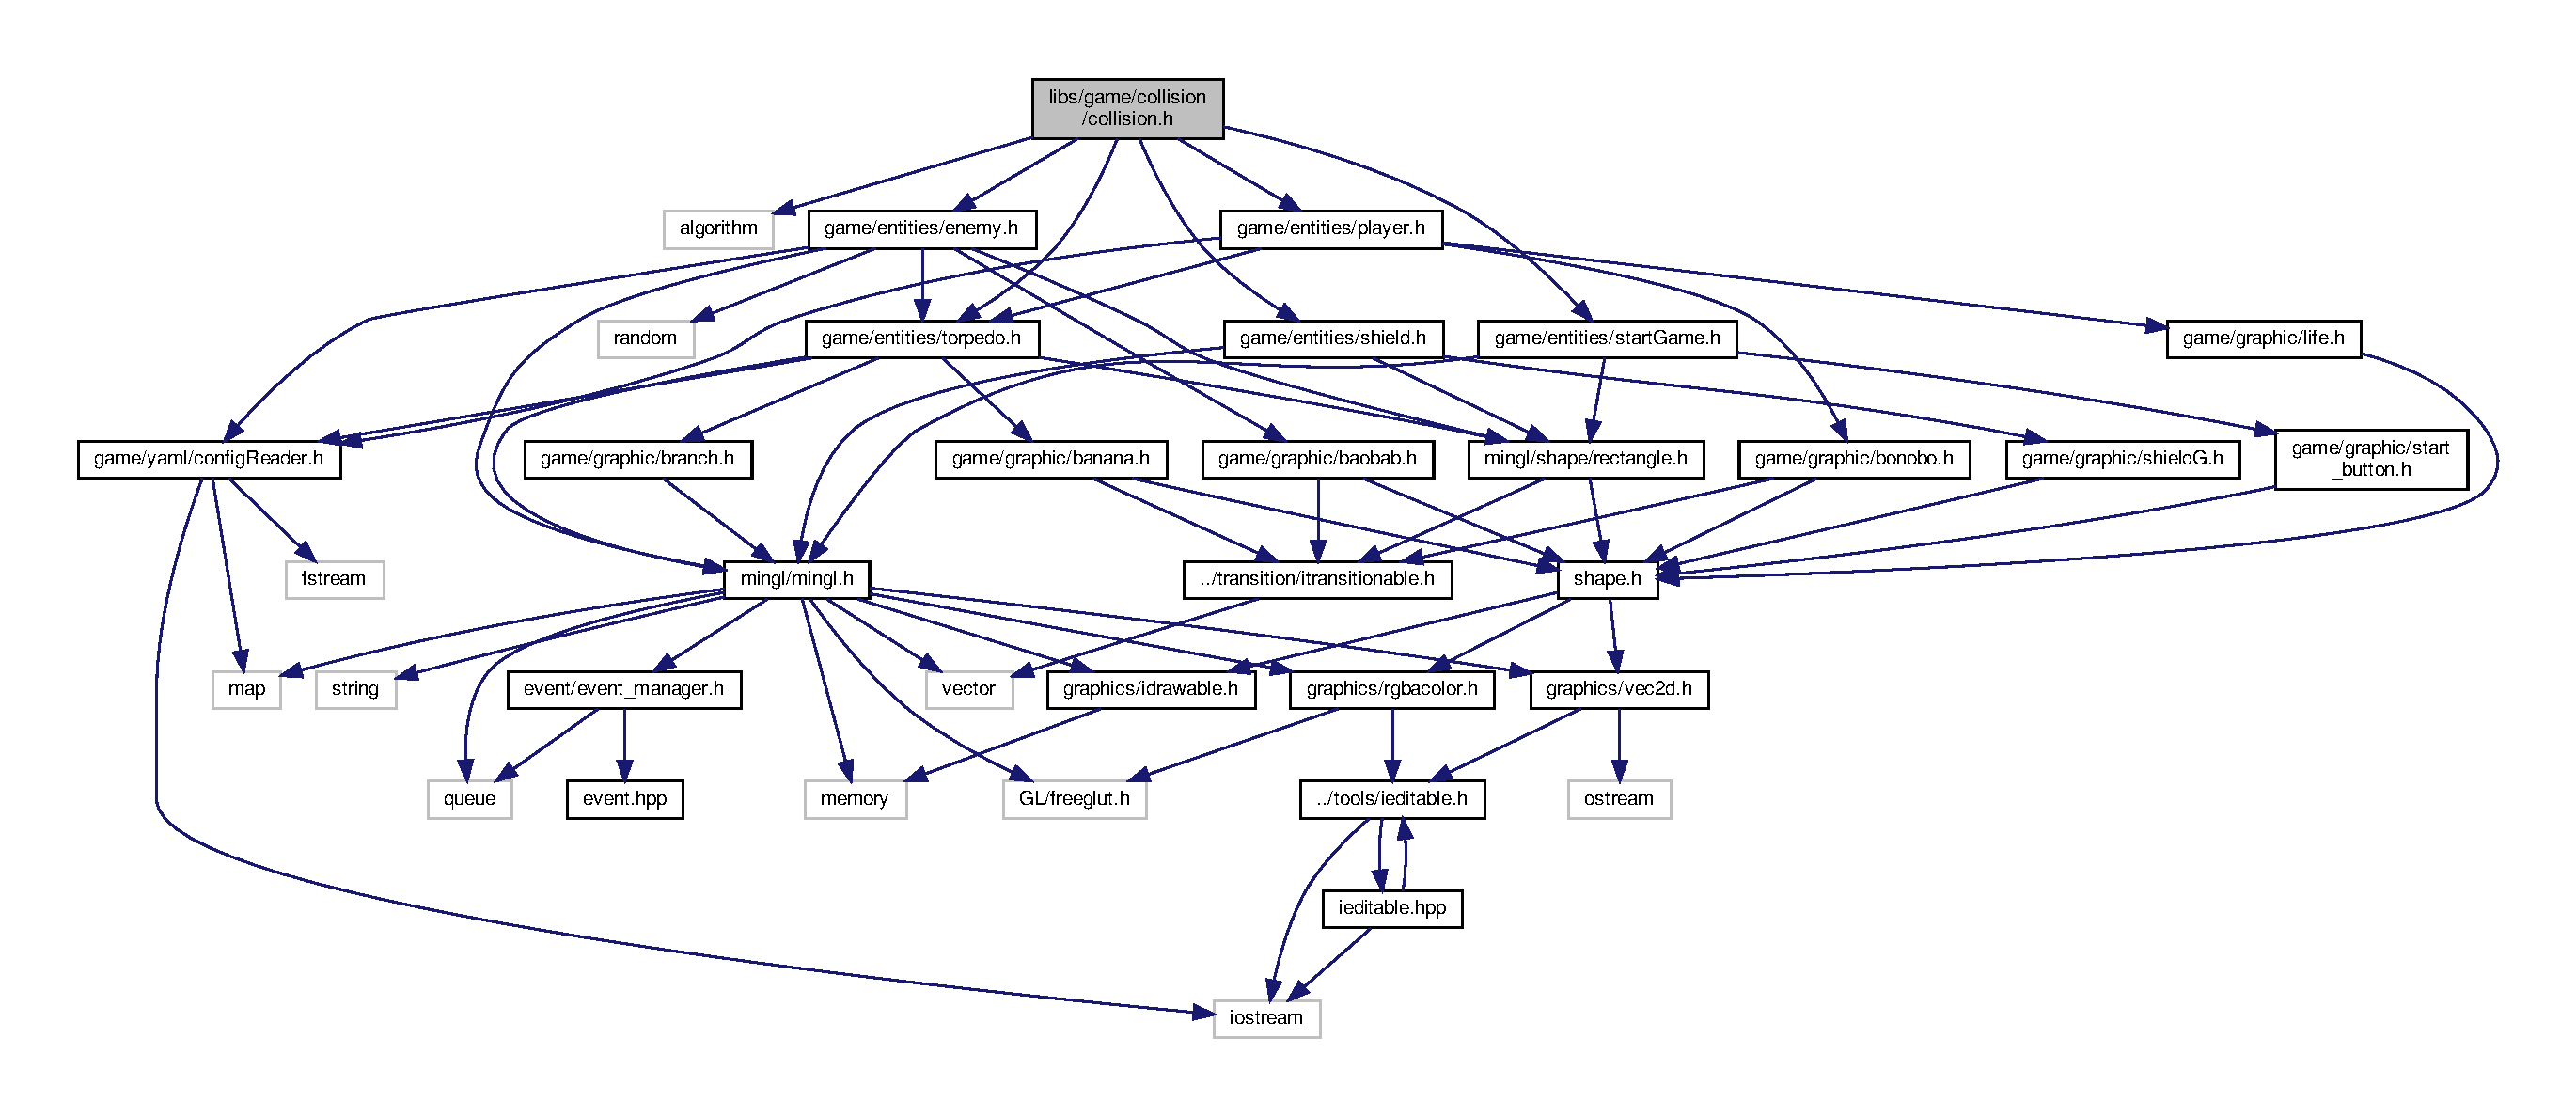
\includegraphics[width=350pt]{collision_8h__incl}
\end{center}
\end{figure}
This graph shows which files directly or indirectly include this file\+:
\nopagebreak
\begin{figure}[H]
\begin{center}
\leavevmode
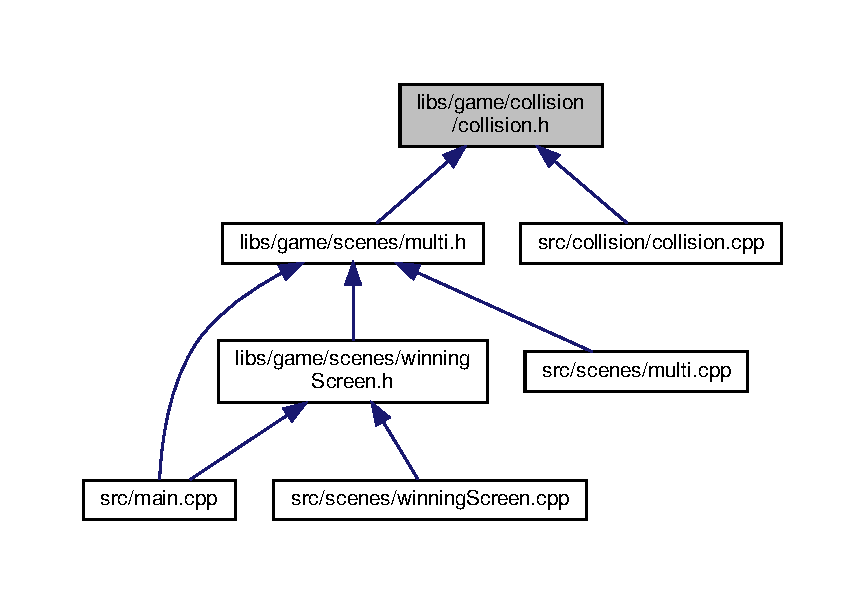
\includegraphics[width=350pt]{collision_8h__dep__incl}
\end{center}
\end{figure}
\subsection*{Namespaces}
\begin{DoxyCompactItemize}
\item 
 \hyperlink{namespacecollision}{collision}
\end{DoxyCompactItemize}
\subsection*{Functions}
\begin{DoxyCompactItemize}
\item 
void \hyperlink{namespacecollision_adede7fb38a79d23854557f97f8a37068}{collision\+::gen\+Coll} (std\+::vector$<$ \hyperlink{structtorpedo_1_1_torpedo}{torpedo\+::\+Torpedo} $>$ \&T, std\+::vector$<$ \hyperlink{structplayer_1_1_player}{player\+::\+Player} $>$ \&P)
\begin{DoxyCompactList}\small\item\em Génère les vecteurs de collisions. \end{DoxyCompactList}\item 
bool \hyperlink{namespacecollision_a84b9e926c787ba05c5b5124ef28ecf88}{collision\+::is\+Colliding} (\hyperlink{classns_graphics_1_1_vec2_d}{ns\+Graphics\+::\+Vec2D} \&pos, \hyperlink{classns_graphics_1_1_vec2_d}{ns\+Graphics\+::\+Vec2D} \&first\+Corner, \hyperlink{classns_graphics_1_1_vec2_d}{ns\+Graphics\+::\+Vec2D} \&second\+Corner)
\begin{DoxyCompactList}\small\item\em Prédicat de collision entre un point et une zone ~\newline
 Cette fonction est équivalente à celle présente dans la bibliothèque \hyperlink{class_min_g_l}{Min\+GL} cependant elle n\textquotesingle{}était pas adapter à notre cas. \end{DoxyCompactList}\item 
void \hyperlink{namespacecollision_a451676809547856fc6f86b3dd6dc7c23}{collision\+::sup\+Double} (std\+::vector$<$ unsigned $>$ \&vec)
\begin{DoxyCompactList}\small\item\em Enlève les doublons dans un tableau trié \end{DoxyCompactList}\item 
std\+::vector$<$ std\+::vector$<$ char $>$ $>$ \hyperlink{namespacecollision_ae1b29fbda8203c6556c2038306ce36e7}{collision\+::collision} (std\+::vector$<$ \hyperlink{structplayer_1_1_player}{player\+::\+Player} $>$ \&\hyperlink{multi_8cpp_abd9de51dc9a6f90588878ff69cec449d}{players}, std\+::vector$<$ \hyperlink{structtorpedo_1_1_torpedo}{torpedo\+::\+Torpedo} $>$ \&\hyperlink{multi_8cpp_a8d978ee3afff71f0b07f921403c2b403}{torpedos}, std\+::vector$<$ \hyperlink{structenemy_1_1_enemy}{enemy\+::\+Enemy} $>$ \&\hyperlink{multi_8cpp_a68dfd8cc6c330a8d7be4cf2f3a6892f3}{enemies}, std\+::vector$<$ \hyperlink{structshield_1_1_shield}{shield\+::\+Shield} $>$ \&\hyperlink{multi_8cpp_a7579d4d68d6c54e66480c4518dd61d70}{shields}, std\+::vector$<$ \hyperlink{structstart_game_1_1_start_game}{start\+Game\+::\+Start\+Game} $>$ \&start\+Game)
\begin{DoxyCompactList}\small\item\em Permet de gérer la collision des entitées. \end{DoxyCompactList}\end{DoxyCompactItemize}


\subsection{Detailed Description}
Permet de gérer les collisions. 

\begin{DoxyAuthor}{Author}
Marius Pistoresi 
\end{DoxyAuthor}
\begin{DoxyDate}{Date}
Décembre 2021 
\end{DoxyDate}
\begin{DoxyVersion}{Version}
1.\+0 
\end{DoxyVersion}

\hypertarget{enemy_8h}{}\section{libs/game/entities/enemy.h File Reference}
\label{enemy_8h}\index{libs/game/entities/enemy.\+h@{libs/game/entities/enemy.\+h}}


Permet de gérer les enemies.  


{\ttfamily \#include \char`\"{}mingl/mingl.\+h\char`\"{}}\newline
{\ttfamily \#include \char`\"{}mingl/shape/rectangle.\+h\char`\"{}}\newline
{\ttfamily \#include \char`\"{}game/yaml/config\+Reader.\+h\char`\"{}}\newline
{\ttfamily \#include \char`\"{}game/entities/torpedo.\+h\char`\"{}}\newline
{\ttfamily \#include $<$random$>$}\newline
{\ttfamily \#include \char`\"{}game/graphic/baobab.\+h\char`\"{}}\newline
Include dependency graph for enemy.\+h\+:
\nopagebreak
\begin{figure}[H]
\begin{center}
\leavevmode
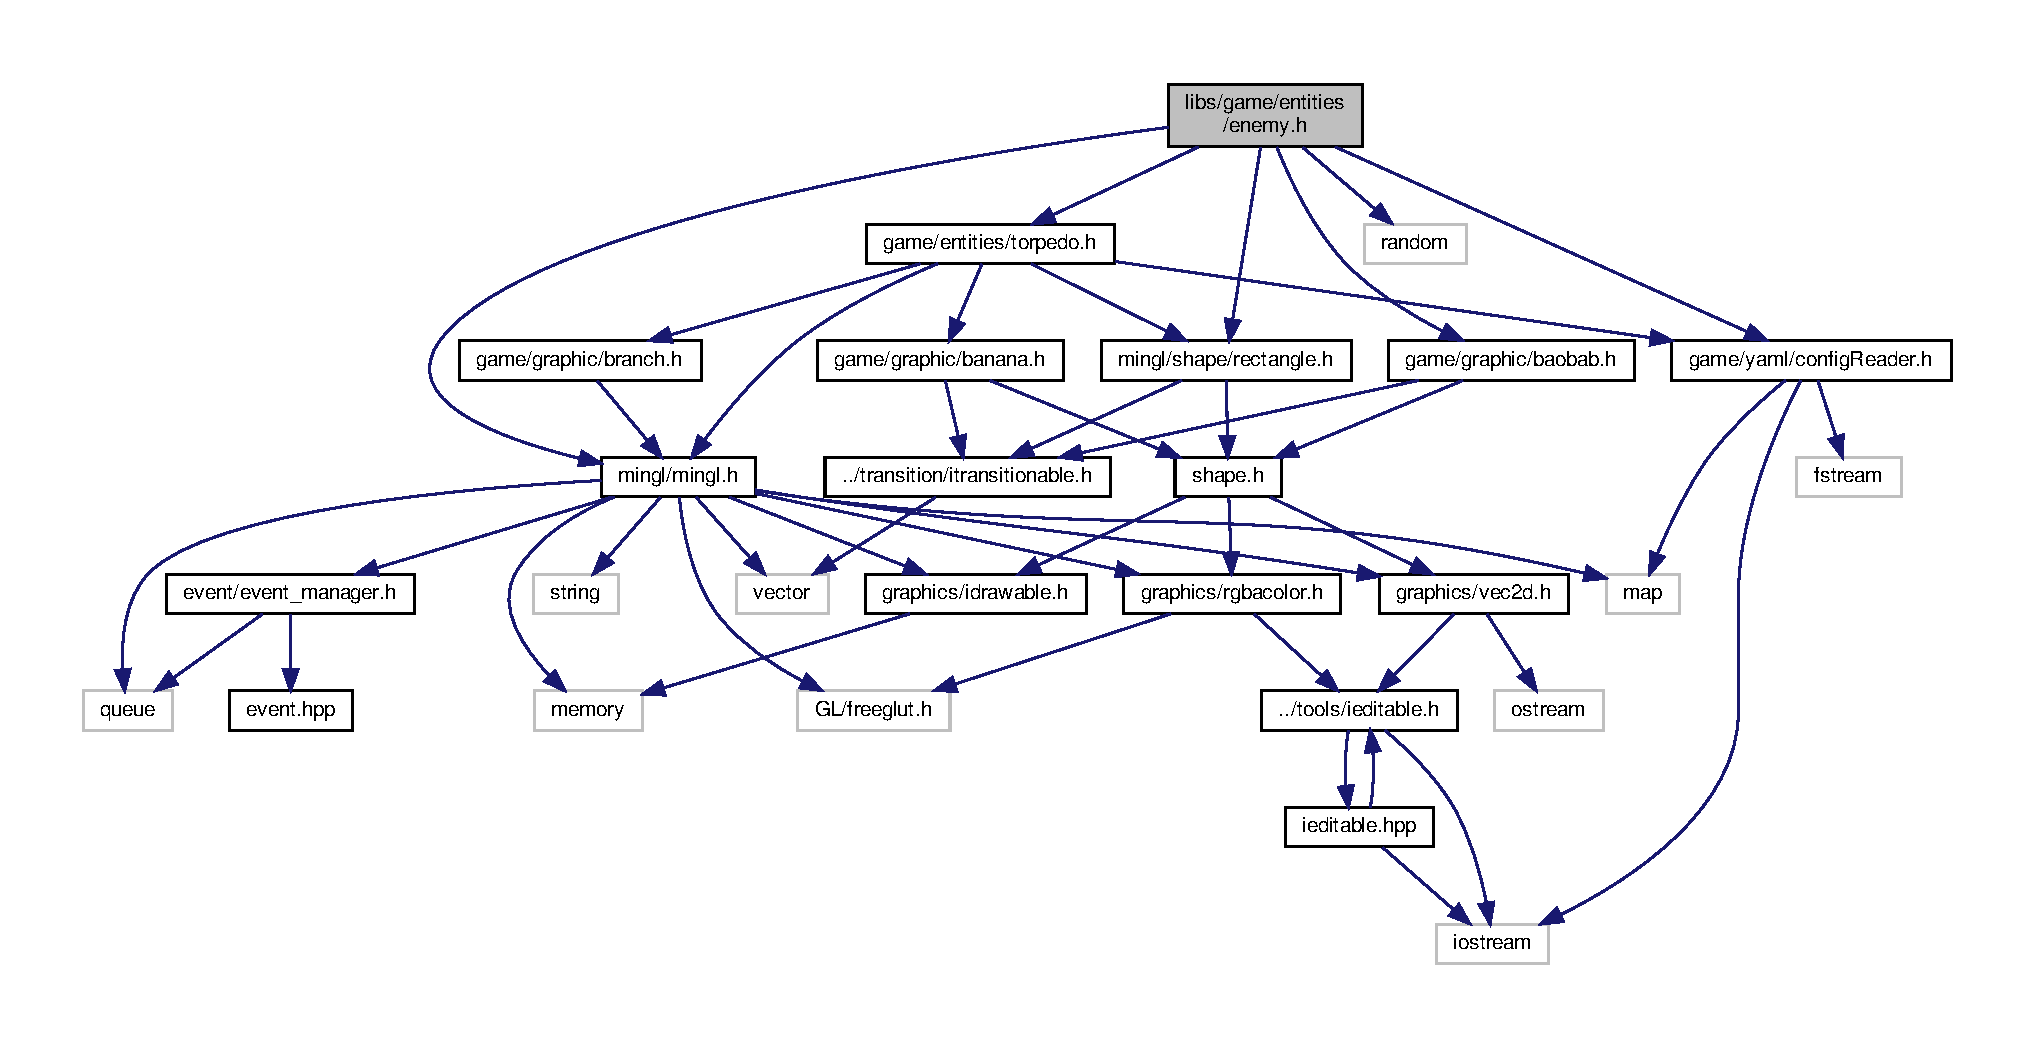
\includegraphics[width=350pt]{enemy_8h__incl}
\end{center}
\end{figure}
This graph shows which files directly or indirectly include this file\+:
\nopagebreak
\begin{figure}[H]
\begin{center}
\leavevmode
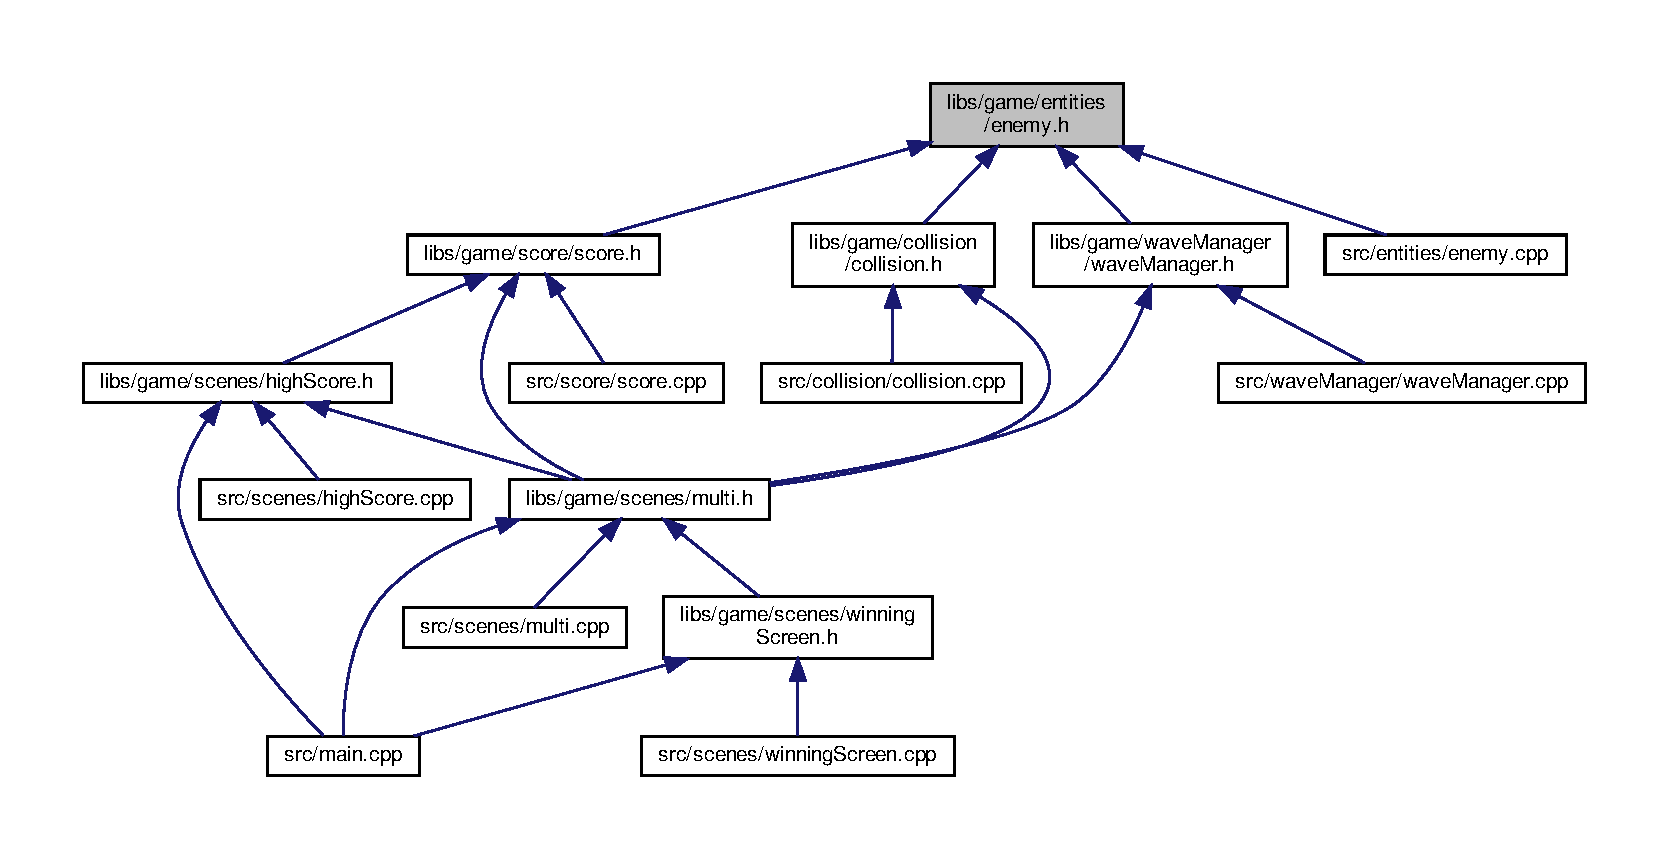
\includegraphics[width=350pt]{enemy_8h__dep__incl}
\end{center}
\end{figure}
\subsection*{Classes}
\begin{DoxyCompactItemize}
\item 
struct \hyperlink{structenemy_1_1_enemy}{enemy\+::\+Enemy}
\begin{DoxyCompactList}\small\item\em Structure d\textquotesingle{}enemies. \end{DoxyCompactList}\end{DoxyCompactItemize}
\subsection*{Namespaces}
\begin{DoxyCompactItemize}
\item 
 \hyperlink{namespaceenemy}{enemy}
\end{DoxyCompactItemize}
\subsection*{Functions}
\begin{DoxyCompactItemize}
\item 
void \hyperlink{namespaceenemy_ac229022d366657680b3b269ca9674734}{enemy\+::init} (std\+::map$<$ std\+::string, std\+::string $>$ \&\hyperlink{main_8cpp_ada2160bcc2082e595d02f0eb5a318dd5}{config\+Map})
\begin{DoxyCompactList}\small\item\em Initialisation de l\textquotesingle{}espace avec la config. \end{DoxyCompactList}\end{DoxyCompactItemize}


\subsection{Detailed Description}
Permet de gérer les enemies. 

\begin{DoxyAuthor}{Author}
Marius Pistoresi 
\end{DoxyAuthor}
\begin{DoxyDate}{Date}
Décembre 2021 
\end{DoxyDate}
\begin{DoxyVersion}{Version}
1.\+0 
\end{DoxyVersion}

\hypertarget{player_8h}{}\section{libs/game/entities/player.h File Reference}
\label{player_8h}\index{libs/game/entities/player.\+h@{libs/game/entities/player.\+h}}


Permet de gérer les joueurs.  


{\ttfamily \#include \char`\"{}game/entities/torpedo.\+h\char`\"{}}\newline
{\ttfamily \#include \char`\"{}game/yaml/config\+Reader.\+h\char`\"{}}\newline
{\ttfamily \#include \char`\"{}game/graphic/bonobo.\+h\char`\"{}}\newline
{\ttfamily \#include \char`\"{}game/graphic/life.\+h\char`\"{}}\newline
Include dependency graph for player.\+h\+:
\nopagebreak
\begin{figure}[H]
\begin{center}
\leavevmode
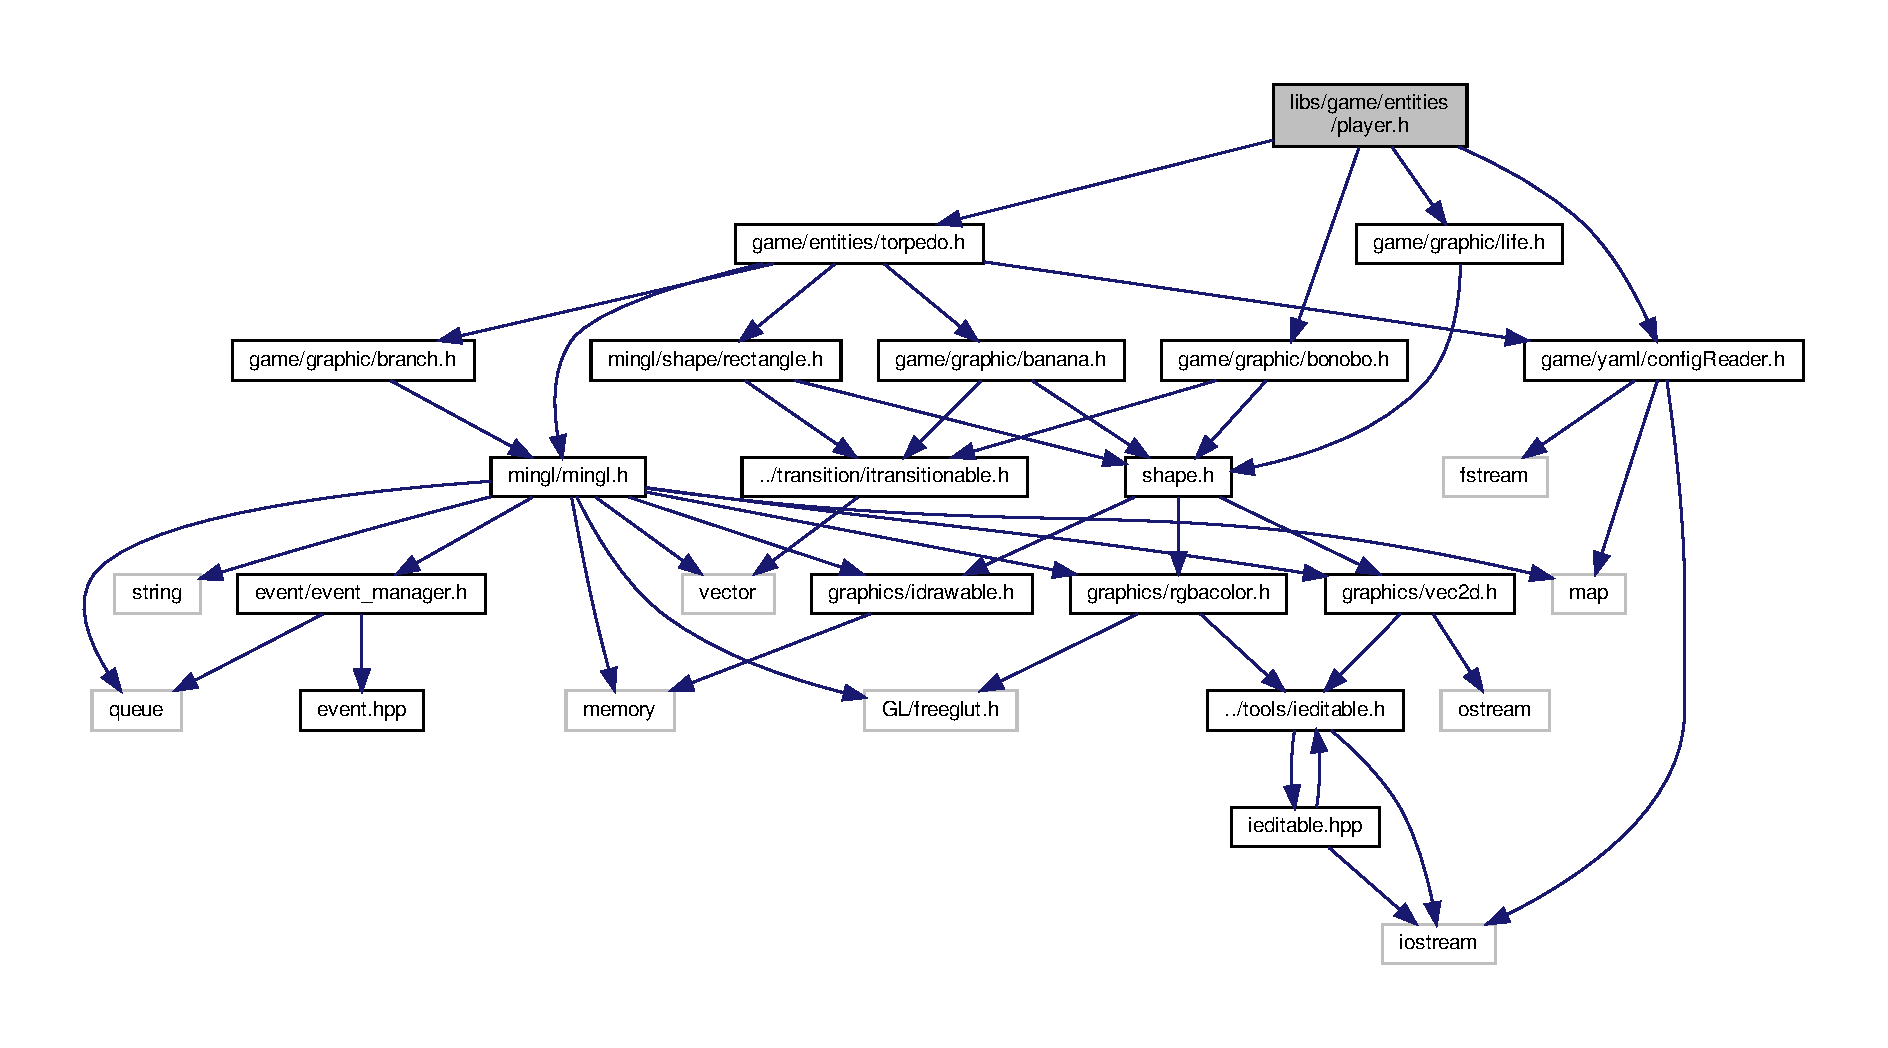
\includegraphics[width=350pt]{player_8h__incl}
\end{center}
\end{figure}
This graph shows which files directly or indirectly include this file\+:
\nopagebreak
\begin{figure}[H]
\begin{center}
\leavevmode
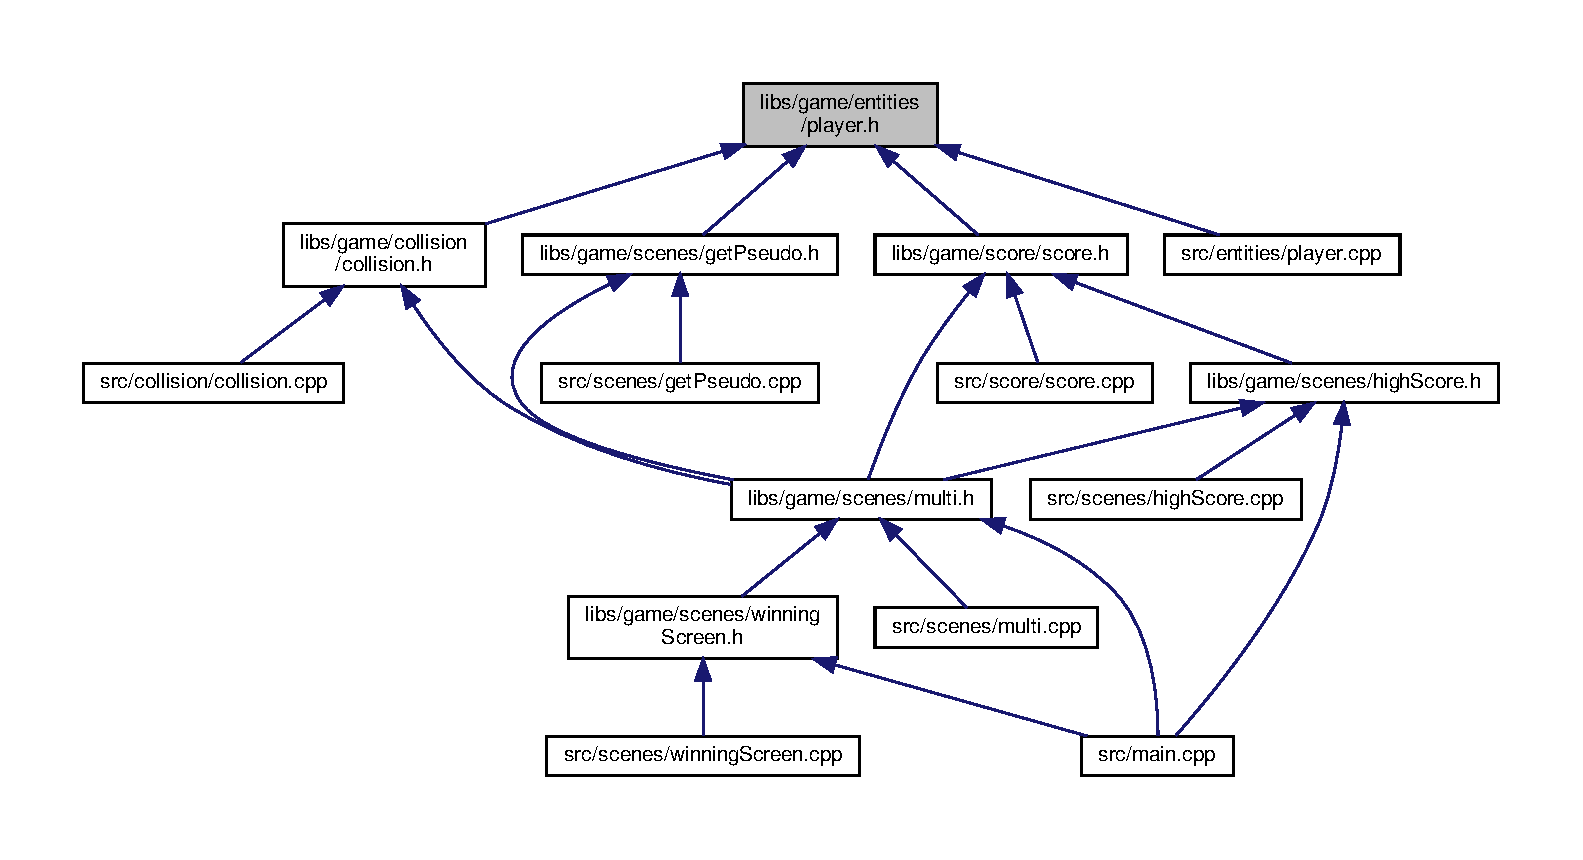
\includegraphics[width=350pt]{player_8h__dep__incl}
\end{center}
\end{figure}
\subsection*{Classes}
\begin{DoxyCompactItemize}
\item 
struct \hyperlink{structplayer_1_1_player}{player\+::\+Player}
\begin{DoxyCompactList}\small\item\em Structure de joueur pour pouvoir les traiter en instance. \end{DoxyCompactList}\end{DoxyCompactItemize}
\subsection*{Namespaces}
\begin{DoxyCompactItemize}
\item 
 \hyperlink{namespaceplayer}{player}
\end{DoxyCompactItemize}
\subsection*{Functions}
\begin{DoxyCompactItemize}
\item 
void \hyperlink{namespaceplayer_a580e093d38d3189329f884f8d69b62c9}{player\+::init} (std\+::map$<$ std\+::string, std\+::string $>$ \&\hyperlink{main_8cpp_ada2160bcc2082e595d02f0eb5a318dd5}{config\+Map})
\begin{DoxyCompactList}\small\item\em Configuration dans l\textquotesingle{}espace vide de la configuration. \end{DoxyCompactList}\end{DoxyCompactItemize}


\subsection{Detailed Description}
Permet de gérer les joueurs. 

\begin{DoxyAuthor}{Author}
Alexis M\+A\+R\+I\+O\+T\+TI $\vert$ Marius P\+I\+S\+T\+O\+R\+E\+SI 
\end{DoxyAuthor}
\begin{DoxyDate}{Date}
Décembre 2021 
\end{DoxyDate}
\begin{DoxyVersion}{Version}
1.\+0 
\end{DoxyVersion}

\hypertarget{shield_8h}{}\section{libs/game/entities/shield.h File Reference}
\label{shield_8h}\index{libs/game/entities/shield.\+h@{libs/game/entities/shield.\+h}}


Permet de gérer les boucliers.  


{\ttfamily \#include \char`\"{}mingl/mingl.\+h\char`\"{}}\newline
{\ttfamily \#include \char`\"{}mingl/shape/rectangle.\+h\char`\"{}}\newline
{\ttfamily \#include \char`\"{}game/graphic/shield\+G.\+h\char`\"{}}\newline
Include dependency graph for shield.\+h\+:
\nopagebreak
\begin{figure}[H]
\begin{center}
\leavevmode
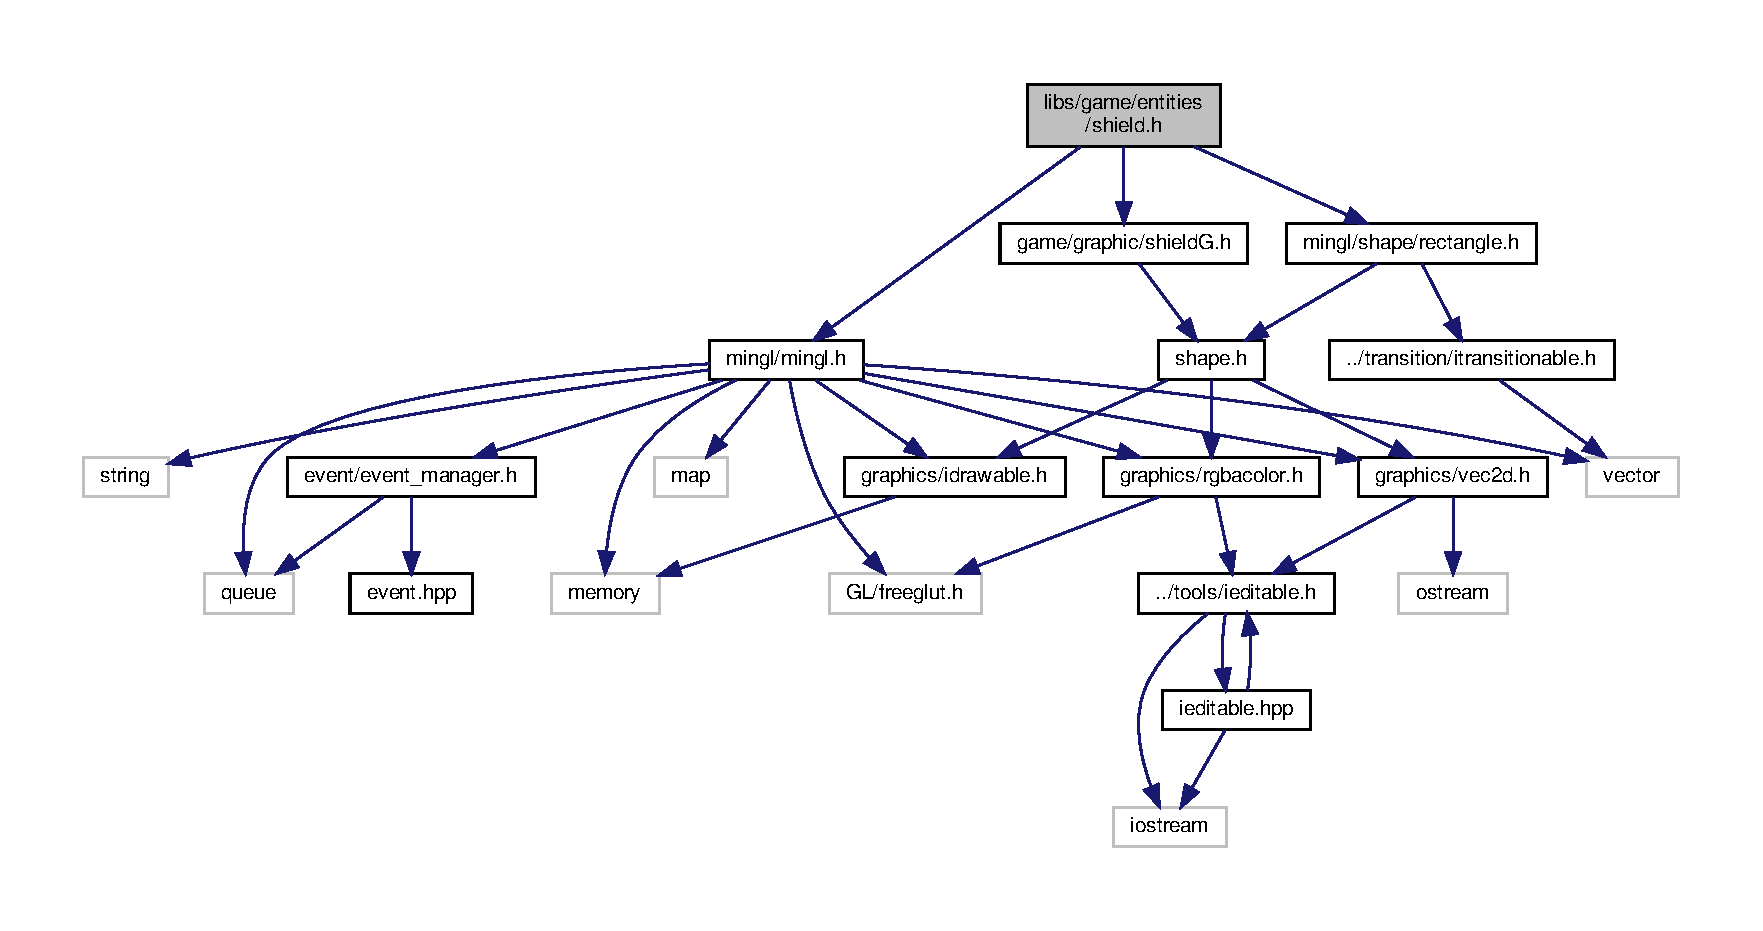
\includegraphics[width=350pt]{shield_8h__incl}
\end{center}
\end{figure}
This graph shows which files directly or indirectly include this file\+:
\nopagebreak
\begin{figure}[H]
\begin{center}
\leavevmode
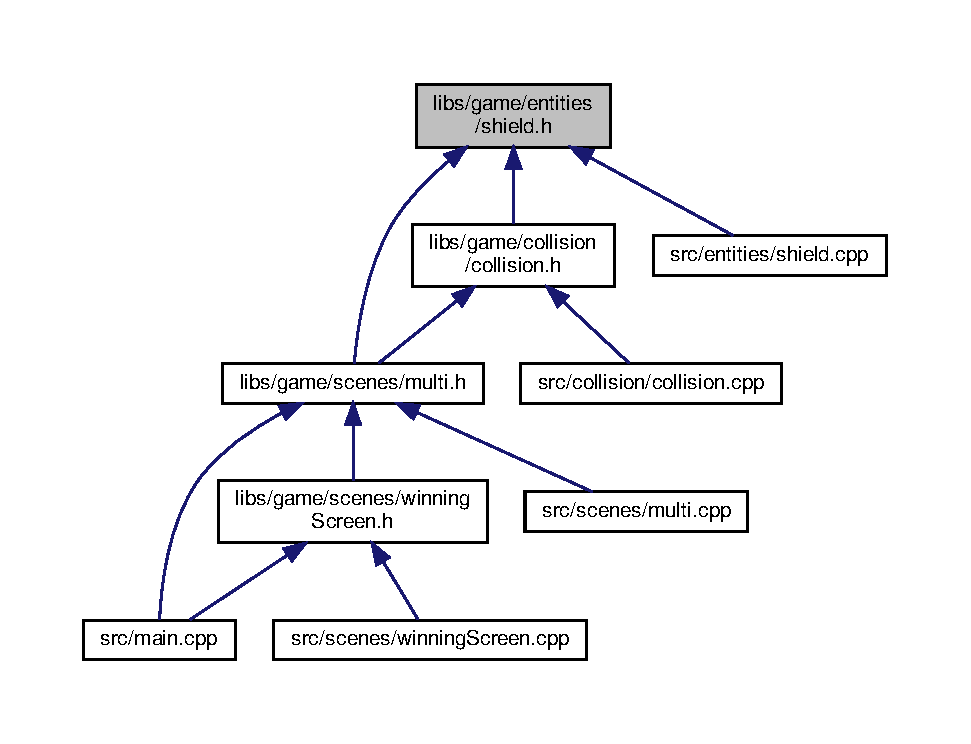
\includegraphics[width=350pt]{shield_8h__dep__incl}
\end{center}
\end{figure}
\subsection*{Classes}
\begin{DoxyCompactItemize}
\item 
struct \hyperlink{structshield_1_1_shield}{shield\+::\+Shield}
\begin{DoxyCompactList}\small\item\em Structure des bouclier. \end{DoxyCompactList}\end{DoxyCompactItemize}
\subsection*{Namespaces}
\begin{DoxyCompactItemize}
\item 
 \hyperlink{namespaceshield}{shield}
\end{DoxyCompactItemize}
\subsection*{Functions}
\begin{DoxyCompactItemize}
\item 
void \hyperlink{namespaceshield_a3545f41f583cca935619e05b604c02e6}{shield\+::gen\+Shield} (std\+::vector$<$ Shield $>$ \&\hyperlink{multi_8cpp_a7579d4d68d6c54e66480c4518dd61d70}{shields}, \hyperlink{class_min_g_l}{Min\+GL} \&window)
\begin{DoxyCompactList}\small\item\em Permet de générer tous les boucliers par rapport à la fenêtre de jeu. \end{DoxyCompactList}\end{DoxyCompactItemize}


\subsection{Detailed Description}
Permet de gérer les boucliers. 

\begin{DoxyAuthor}{Author}
Marius P\+I\+S\+T\+O\+R\+E\+SI 
\end{DoxyAuthor}
\begin{DoxyDate}{Date}
Janvier 2022 
\end{DoxyDate}
\begin{DoxyVersion}{Version}
1.\+0 
\end{DoxyVersion}

\hypertarget{start_game_8h}{}\section{libs/game/entities/start\+Game.h File Reference}
\label{start_game_8h}\index{libs/game/entities/start\+Game.\+h@{libs/game/entities/start\+Game.\+h}}


Permet de gérer le départ d\textquotesingle{}une partie.  


{\ttfamily \#include \char`\"{}mingl/mingl.\+h\char`\"{}}\newline
{\ttfamily \#include \char`\"{}mingl/shape/rectangle.\+h\char`\"{}}\newline
{\ttfamily \#include \char`\"{}game/graphic/start\+\_\+button.\+h\char`\"{}}\newline
Include dependency graph for start\+Game.\+h\+:
\nopagebreak
\begin{figure}[H]
\begin{center}
\leavevmode
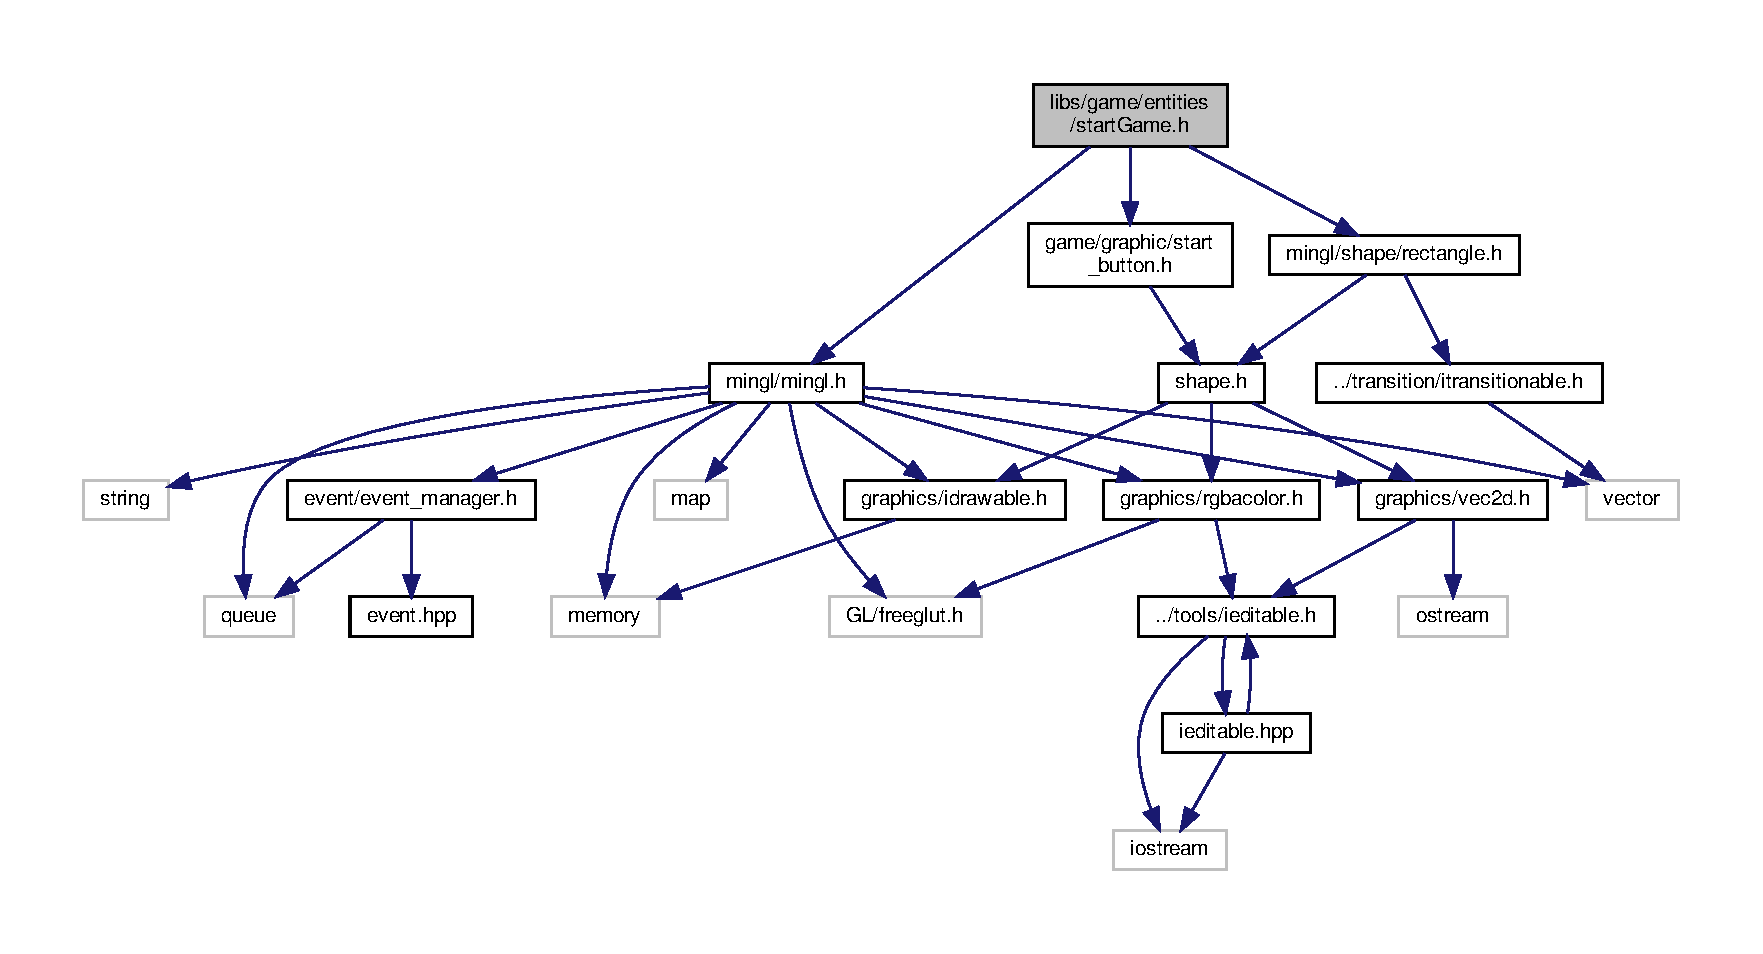
\includegraphics[width=350pt]{start_game_8h__incl}
\end{center}
\end{figure}
This graph shows which files directly or indirectly include this file\+:
\nopagebreak
\begin{figure}[H]
\begin{center}
\leavevmode
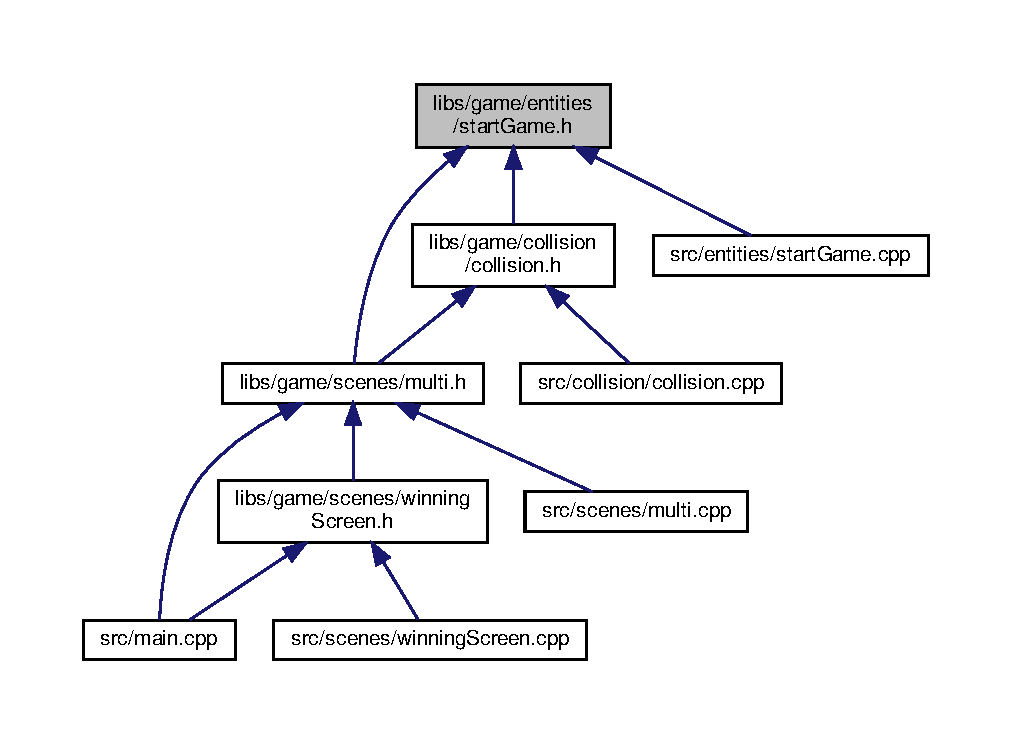
\includegraphics[width=350pt]{start_game_8h__dep__incl}
\end{center}
\end{figure}
\subsection*{Classes}
\begin{DoxyCompactItemize}
\item 
struct \hyperlink{structstart_game_1_1_start_game}{start\+Game\+::\+Start\+Game}
\begin{DoxyCompactList}\small\item\em Structure du départ de la partie. \end{DoxyCompactList}\end{DoxyCompactItemize}
\subsection*{Namespaces}
\begin{DoxyCompactItemize}
\item 
 \hyperlink{namespacestart_game}{start\+Game}
\end{DoxyCompactItemize}


\subsection{Detailed Description}
Permet de gérer le départ d\textquotesingle{}une partie. 

\begin{DoxyAuthor}{Author}
Marius P\+I\+S\+T\+O\+R\+E\+SI 
\end{DoxyAuthor}
\begin{DoxyDate}{Date}
Decembre 2021 
\end{DoxyDate}
\begin{DoxyVersion}{Version}
1.\+0 
\end{DoxyVersion}

\hypertarget{torpedo_8h}{}\section{libs/game/entities/torpedo.h File Reference}
\label{torpedo_8h}\index{libs/game/entities/torpedo.\+h@{libs/game/entities/torpedo.\+h}}
{\ttfamily \#include \char`\"{}mingl/mingl.\+h\char`\"{}}\newline
{\ttfamily \#include \char`\"{}mingl/shape/rectangle.\+h\char`\"{}}\newline
{\ttfamily \#include \char`\"{}game/yaml/config\+Reader.\+h\char`\"{}}\newline
{\ttfamily \#include \char`\"{}game/graphic/branch.\+h\char`\"{}}\newline
{\ttfamily \#include \char`\"{}game/graphic/banana.\+h\char`\"{}}\newline
Include dependency graph for torpedo.\+h\+:
\nopagebreak
\begin{figure}[H]
\begin{center}
\leavevmode
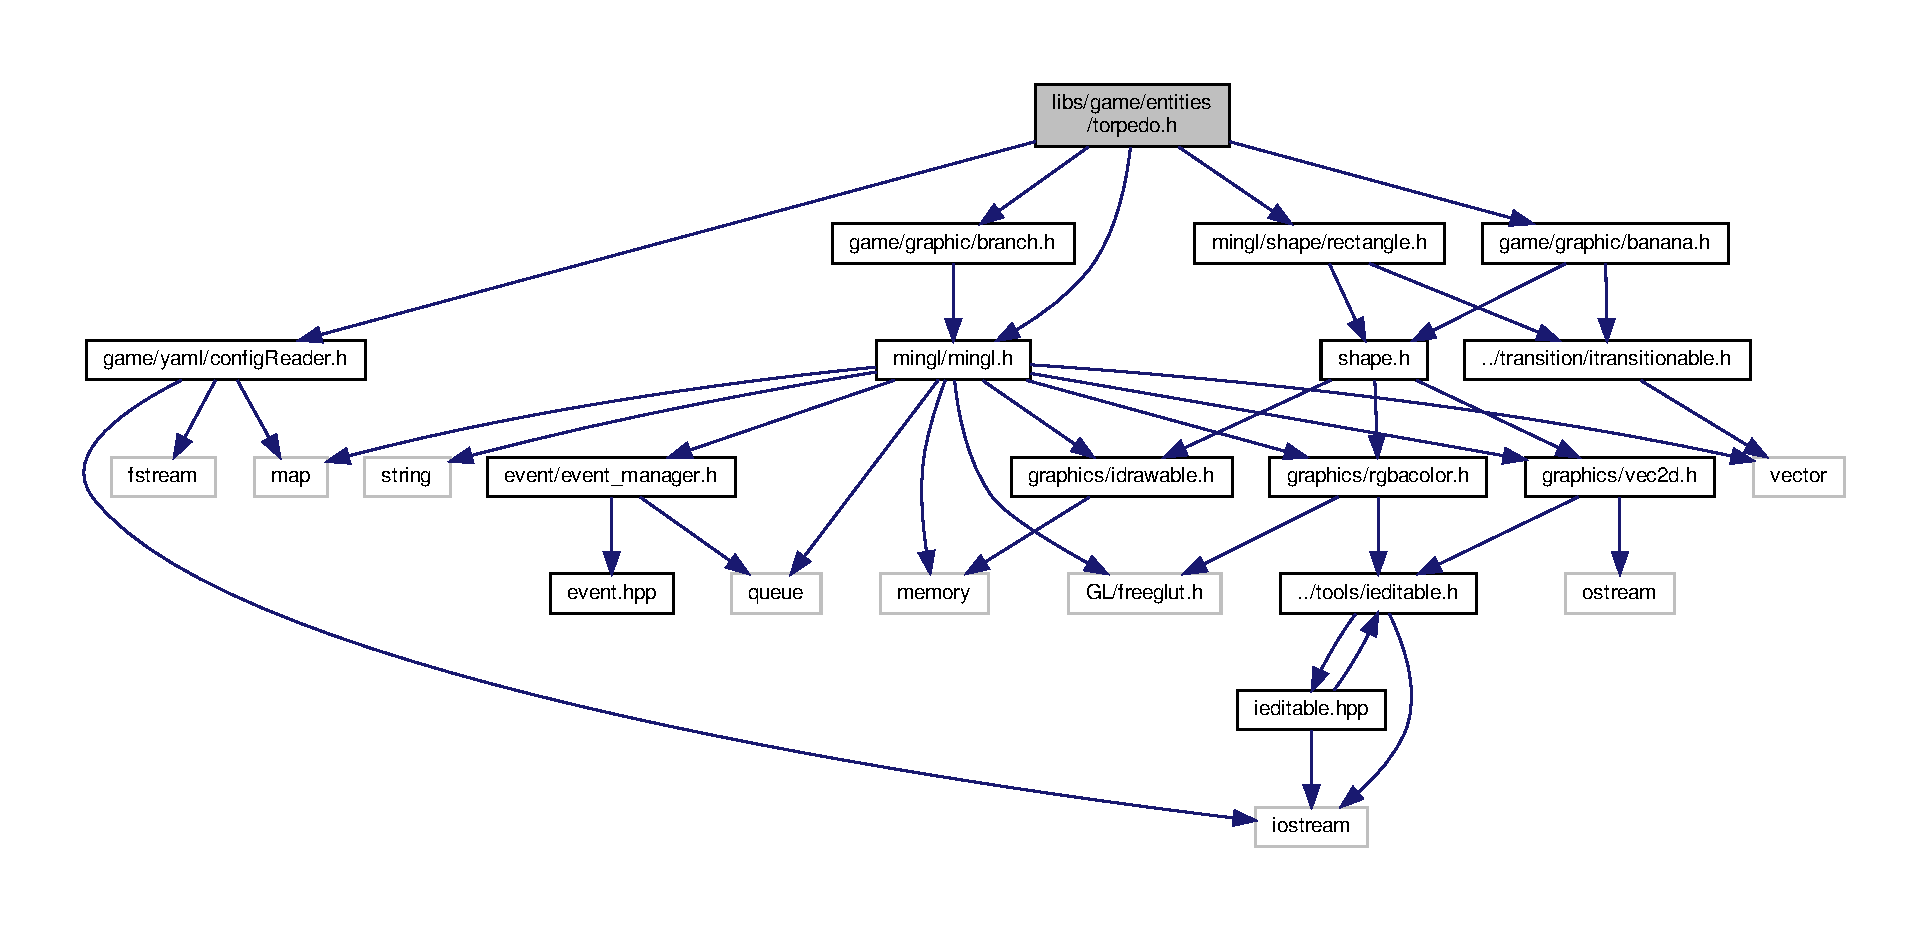
\includegraphics[width=350pt]{torpedo_8h__incl}
\end{center}
\end{figure}
This graph shows which files directly or indirectly include this file\+:
\nopagebreak
\begin{figure}[H]
\begin{center}
\leavevmode
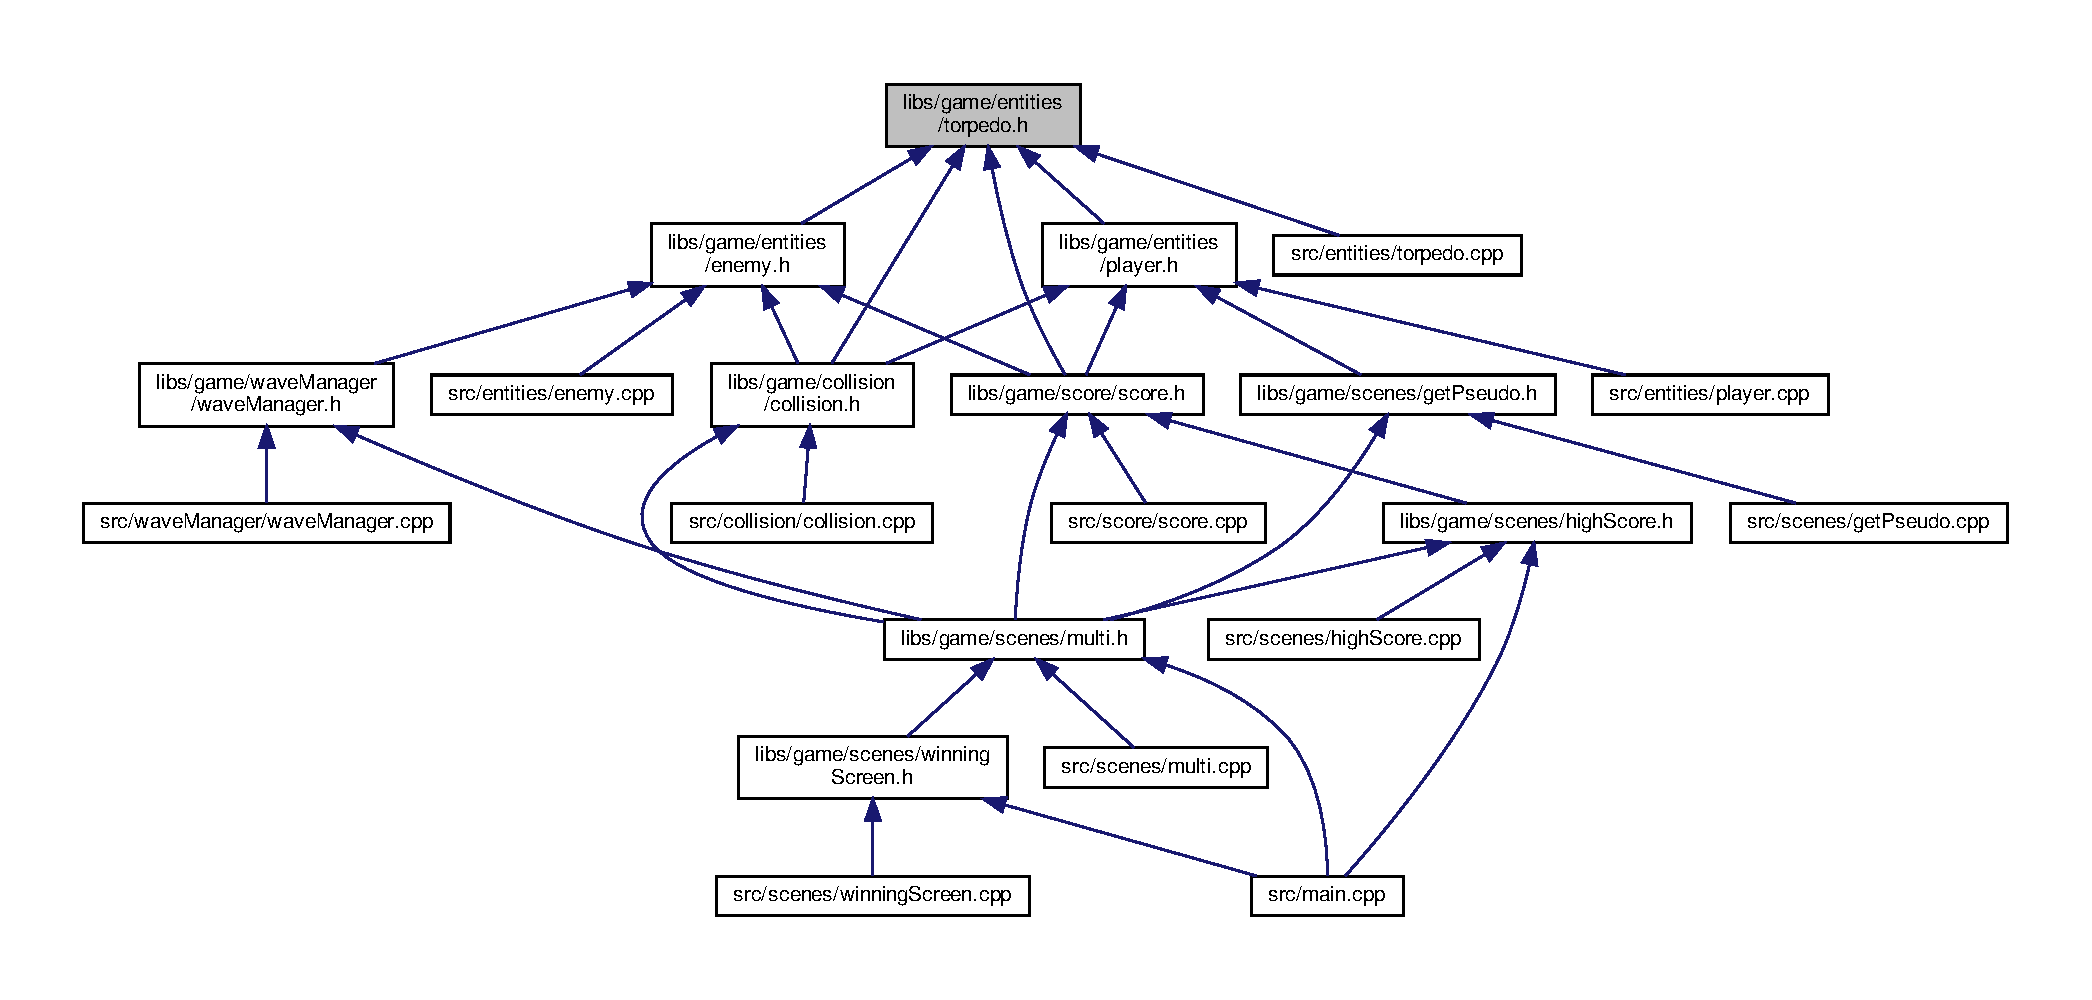
\includegraphics[width=350pt]{torpedo_8h__dep__incl}
\end{center}
\end{figure}
\subsection*{Classes}
\begin{DoxyCompactItemize}
\item 
struct \hyperlink{structtorpedo_1_1_torpedo}{torpedo\+::\+Torpedo}
\begin{DoxyCompactList}\small\item\em Structure pour les torpilles. \end{DoxyCompactList}\end{DoxyCompactItemize}
\subsection*{Namespaces}
\begin{DoxyCompactItemize}
\item 
 \hyperlink{namespacetorpedo}{torpedo}
\end{DoxyCompactItemize}
\subsection*{Functions}
\begin{DoxyCompactItemize}
\item 
void \hyperlink{namespacetorpedo_ad2f33d6b4c7571ef3013ab1b7db70a8b}{torpedo\+::init} (std\+::map$<$ std\+::string, std\+::string $>$ \&\hyperlink{main_8cpp_ada2160bcc2082e595d02f0eb5a318dd5}{config\+Map})
\begin{DoxyCompactList}\small\item\em Permet de gérer la configuration dans l\textquotesingle{}espace vide. \end{DoxyCompactList}\end{DoxyCompactItemize}

\hypertarget{arc__circle_8h}{}\section{libs/game/graphic/arc\+\_\+circle.h File Reference}
\label{arc__circle_8h}\index{libs/game/graphic/arc\+\_\+circle.\+h@{libs/game/graphic/arc\+\_\+circle.\+h}}


Représente un arc de cercle.  


{\ttfamily \#include \char`\"{}mingl/shape/shape.\+h\char`\"{}}\newline
{\ttfamily \#include $<$cmath$>$}\newline
{\ttfamily \#include \char`\"{}mingl/macros.\+h\char`\"{}}\newline
{\ttfamily \#include \char`\"{}mingl/transition/itransitionable.\+h\char`\"{}}\newline
Include dependency graph for arc\+\_\+circle.\+h\+:
\nopagebreak
\begin{figure}[H]
\begin{center}
\leavevmode
\includegraphics[width=350pt]{arc__circle_8h__incl}
\end{center}
\end{figure}
This graph shows which files directly or indirectly include this file\+:
\nopagebreak
\begin{figure}[H]
\begin{center}
\leavevmode
\includegraphics[width=350pt]{arc__circle_8h__dep__incl}
\end{center}
\end{figure}
\subsection*{Classes}
\begin{DoxyCompactItemize}
\item 
class \hyperlink{classns_shape_1_1_arc___circle}{ns\+Shape\+::\+Arc\+\_\+\+Circle}
\begin{DoxyCompactList}\small\item\em Classe représentant un arc de cercle. \end{DoxyCompactList}\end{DoxyCompactItemize}
\subsection*{Namespaces}
\begin{DoxyCompactItemize}
\item 
 \hyperlink{namespacens_shape}{ns\+Shape}
\begin{DoxyCompactList}\small\item\em Espace de nom pour différentes formes. \end{DoxyCompactList}\end{DoxyCompactItemize}


\subsection{Detailed Description}
Représente un arc de cercle. 

\begin{DoxyAuthor}{Author}
M\+E\+T\+A\+Y\+ER S\+L\+O\+A\+NE 
\end{DoxyAuthor}
\begin{DoxyDate}{Date}
Decembre 2021 
\end{DoxyDate}
\begin{DoxyVersion}{Version}
1.\+0.\+1 
\end{DoxyVersion}

\hypertarget{banana_8h}{}\section{libs/game/graphic/banana.h File Reference}
\label{banana_8h}\index{libs/game/graphic/banana.\+h@{libs/game/graphic/banana.\+h}}


Représente une banane.  


{\ttfamily \#include \char`\"{}mingl/shape/shape.\+h\char`\"{}}\newline
{\ttfamily \#include \char`\"{}mingl/transition/itransitionable.\+h\char`\"{}}\newline
Include dependency graph for banana.\+h\+:
\nopagebreak
\begin{figure}[H]
\begin{center}
\leavevmode
\includegraphics[width=350pt]{banana_8h__incl}
\end{center}
\end{figure}
This graph shows which files directly or indirectly include this file\+:
\nopagebreak
\begin{figure}[H]
\begin{center}
\leavevmode
\includegraphics[width=350pt]{banana_8h__dep__incl}
\end{center}
\end{figure}
\subsection*{Namespaces}
\begin{DoxyCompactItemize}
\item 
 \hyperlink{namespacebanana}{banana}
\end{DoxyCompactItemize}
\subsection*{Functions}
\begin{DoxyCompactItemize}
\item 
void \hyperlink{namespacebanana_a3c2a9734db3a61dd188f96524cdcc160}{banana\+::draw} (\hyperlink{class_min_g_l}{Min\+GL} \&window, \hyperlink{classns_graphics_1_1_vec2_d}{ns\+Graphics\+::\+Vec2D} pos, unsigned size, char direction)
\end{DoxyCompactItemize}


\subsection{Detailed Description}
Représente une banane. 

\begin{DoxyAuthor}{Author}
E\+G\+E\+N\+S\+C\+H\+E\+V\+I\+L\+L\+ER F\+R\+E\+D\+E\+R\+IC 
\end{DoxyAuthor}
\begin{DoxyDate}{Date}
Décembre 2021 
\end{DoxyDate}
\begin{DoxyVersion}{Version}
1.\+0.\+1 
\end{DoxyVersion}

\hypertarget{baobab_8h}{}\section{libs/game/graphic/baobab.h File Reference}
\label{baobab_8h}\index{libs/game/graphic/baobab.\+h@{libs/game/graphic/baobab.\+h}}


Représente un baobab.  


{\ttfamily \#include \char`\"{}mingl/shape/shape.\+h\char`\"{}}\newline
{\ttfamily \#include \char`\"{}mingl/transition/itransitionable.\+h\char`\"{}}\newline
Include dependency graph for baobab.\+h\+:
\nopagebreak
\begin{figure}[H]
\begin{center}
\leavevmode
\includegraphics[width=350pt]{baobab_8h__incl}
\end{center}
\end{figure}
This graph shows which files directly or indirectly include this file\+:
\nopagebreak
\begin{figure}[H]
\begin{center}
\leavevmode
\includegraphics[width=350pt]{baobab_8h__dep__incl}
\end{center}
\end{figure}
\subsection*{Namespaces}
\begin{DoxyCompactItemize}
\item 
 \hyperlink{namespacebaobab}{baobab}
\end{DoxyCompactItemize}
\subsection*{Functions}
\begin{DoxyCompactItemize}
\item 
void \hyperlink{namespacebaobab_aeb5d6068d067244665b248a84790769e}{baobab\+::draw} (\hyperlink{class_min_g_l}{Min\+GL} \&window, \hyperlink{classns_graphics_1_1_vec2_d}{ns\+Graphics\+::\+Vec2D} pos, unsigned size)
\end{DoxyCompactItemize}


\subsection{Detailed Description}
Représente un baobab. 

\begin{DoxyAuthor}{Author}
M\+E\+T\+A\+Y\+ER S\+L\+O\+A\+NE 
\end{DoxyAuthor}
\begin{DoxyDate}{Date}
Décembre 2021 
\end{DoxyDate}
\begin{DoxyVersion}{Version}
1.\+0.\+1 
\end{DoxyVersion}

\hypertarget{bonobo_8h}{}\section{libs/game/graphic/bonobo.h File Reference}
\label{bonobo_8h}\index{libs/game/graphic/bonobo.\+h@{libs/game/graphic/bonobo.\+h}}


Représente un bonobo.  


{\ttfamily \#include \char`\"{}mingl/shape/shape.\+h\char`\"{}}\newline
{\ttfamily \#include \char`\"{}mingl/transition/itransitionable.\+h\char`\"{}}\newline
Include dependency graph for bonobo.\+h\+:
\nopagebreak
\begin{figure}[H]
\begin{center}
\leavevmode
\includegraphics[width=350pt]{bonobo_8h__incl}
\end{center}
\end{figure}
This graph shows which files directly or indirectly include this file\+:
\nopagebreak
\begin{figure}[H]
\begin{center}
\leavevmode
\includegraphics[width=350pt]{bonobo_8h__dep__incl}
\end{center}
\end{figure}
\subsection*{Namespaces}
\begin{DoxyCompactItemize}
\item 
 \hyperlink{namespacebonobo}{bonobo}
\end{DoxyCompactItemize}
\subsection*{Functions}
\begin{DoxyCompactItemize}
\item 
void \hyperlink{namespacebonobo_ad8bf46cc96e04a00d58e925eb50130b5}{bonobo\+::draw} (\hyperlink{class_min_g_l}{Min\+GL} \&window, \hyperlink{classns_graphics_1_1_vec2_d}{ns\+Graphics\+::\+Vec2D} \&pos, unsigned radius)
\end{DoxyCompactItemize}


\subsection{Detailed Description}
Représente un bonobo. 

\begin{DoxyAuthor}{Author}
E\+G\+E\+N\+S\+C\+H\+E\+V\+I\+L\+L\+ER F\+R\+E\+D\+E\+R\+IC 
\end{DoxyAuthor}
\begin{DoxyDate}{Date}
Décembre 2021 
\end{DoxyDate}
\begin{DoxyVersion}{Version}
1.\+0.\+1 
\end{DoxyVersion}

\hypertarget{branch_8h}{}\section{libs/game/graphic/branch.h File Reference}
\label{branch_8h}\index{libs/game/graphic/branch.\+h@{libs/game/graphic/branch.\+h}}


Représente une branche.  


{\ttfamily \#include \char`\"{}mingl/mingl.\+h\char`\"{}}\newline
Include dependency graph for branch.\+h\+:
\nopagebreak
\begin{figure}[H]
\begin{center}
\leavevmode
\includegraphics[width=350pt]{branch_8h__incl}
\end{center}
\end{figure}
This graph shows which files directly or indirectly include this file\+:
\nopagebreak
\begin{figure}[H]
\begin{center}
\leavevmode
\includegraphics[width=350pt]{branch_8h__dep__incl}
\end{center}
\end{figure}
\subsection*{Namespaces}
\begin{DoxyCompactItemize}
\item 
 \hyperlink{namespacebranch}{branch}
\end{DoxyCompactItemize}
\subsection*{Functions}
\begin{DoxyCompactItemize}
\item 
void \hyperlink{namespacebranch_a3c8d57c5c98ab9210a8bc3e60915cd88}{branch\+::draw} (\hyperlink{class_min_g_l}{Min\+GL} \&window, \hyperlink{classns_graphics_1_1_vec2_d}{ns\+Graphics\+::\+Vec2D} pos, unsigned size)
\end{DoxyCompactItemize}


\subsection{Detailed Description}
Représente une branche. 

\begin{DoxyAuthor}{Author}
M\+E\+T\+A\+Y\+ER S\+L\+O\+A\+NE 
\end{DoxyAuthor}
\begin{DoxyDate}{Date}
Decembre 2021 
\end{DoxyDate}
\begin{DoxyVersion}{Version}
1.\+0.\+1 
\end{DoxyVersion}

\hypertarget{credit__button_8h}{}\section{libs/game/graphic/credit\+\_\+button.h File Reference}
\label{credit__button_8h}\index{libs/game/graphic/credit\+\_\+button.\+h@{libs/game/graphic/credit\+\_\+button.\+h}}


Représente le bouton de crédit.  


{\ttfamily \#include \char`\"{}mingl/shape/shape.\+h\char`\"{}}\newline
{\ttfamily \#include \char`\"{}mingl/transition/itransitionable.\+h\char`\"{}}\newline
Include dependency graph for credit\+\_\+button.\+h\+:
\nopagebreak
\begin{figure}[H]
\begin{center}
\leavevmode
\includegraphics[width=350pt]{credit__button_8h__incl}
\end{center}
\end{figure}
This graph shows which files directly or indirectly include this file\+:
\nopagebreak
\begin{figure}[H]
\begin{center}
\leavevmode
\includegraphics[width=346pt]{credit__button_8h__dep__incl}
\end{center}
\end{figure}
\subsection*{Namespaces}
\begin{DoxyCompactItemize}
\item 
 \hyperlink{namespacecredit__button}{credit\+\_\+button}
\end{DoxyCompactItemize}
\subsection*{Functions}
\begin{DoxyCompactItemize}
\item 
void \hyperlink{namespacecredit__button_a7d963523001d9e76bf80d3a344478b64}{credit\+\_\+button\+::draw} (\hyperlink{class_min_g_l}{Min\+GL} \&window, \hyperlink{classns_graphics_1_1_vec2_d}{ns\+Graphics\+::\+Vec2D} pos, unsigned size, char state)
\end{DoxyCompactItemize}


\subsection{Detailed Description}
Représente le bouton de crédit. 

\begin{DoxyAuthor}{Author}
E\+G\+E\+N\+S\+C\+H\+E\+V\+I\+L\+L\+ER F\+R\+E\+D\+E\+R\+IC 
\end{DoxyAuthor}
\begin{DoxyDate}{Date}
Decembre 2021 
\end{DoxyDate}
\begin{DoxyVersion}{Version}
1.\+0.\+1 
\end{DoxyVersion}

\hypertarget{exit__button_8h}{}\section{libs/game/graphic/exit\+\_\+button.h File Reference}
\label{exit__button_8h}\index{libs/game/graphic/exit\+\_\+button.\+h@{libs/game/graphic/exit\+\_\+button.\+h}}


Représente un bouton de sortie.  


{\ttfamily \#include \char`\"{}mingl/shape/shape.\+h\char`\"{}}\newline
{\ttfamily \#include \char`\"{}mingl/transition/itransitionable.\+h\char`\"{}}\newline
Include dependency graph for exit\+\_\+button.\+h\+:
\nopagebreak
\begin{figure}[H]
\begin{center}
\leavevmode
\includegraphics[width=350pt]{exit__button_8h__incl}
\end{center}
\end{figure}
This graph shows which files directly or indirectly include this file\+:
\nopagebreak
\begin{figure}[H]
\begin{center}
\leavevmode
\includegraphics[width=350pt]{exit__button_8h__dep__incl}
\end{center}
\end{figure}
\subsection*{Namespaces}
\begin{DoxyCompactItemize}
\item 
 \hyperlink{namespaceexit__button}{exit\+\_\+button}
\end{DoxyCompactItemize}
\subsection*{Functions}
\begin{DoxyCompactItemize}
\item 
void \hyperlink{namespaceexit__button_adbc23adf7aa51480b13432f5e3c397b6}{exit\+\_\+button\+::draw} (\hyperlink{class_min_g_l}{Min\+GL} \&window, \hyperlink{classns_graphics_1_1_vec2_d}{ns\+Graphics\+::\+Vec2D} pos, unsigned size, char state)
\end{DoxyCompactItemize}


\subsection{Detailed Description}
Représente un bouton de sortie. 

\begin{DoxyAuthor}{Author}
M\+E\+T\+A\+Y\+ER S\+L\+O\+A\+NE 
\end{DoxyAuthor}
\begin{DoxyDate}{Date}
Decembre 2021 
\end{DoxyDate}
\begin{DoxyVersion}{Version}
1.\+0.\+1 
\end{DoxyVersion}

\hypertarget{half__circle_8h}{}\section{libs/game/graphic/half\+\_\+circle.h File Reference}
\label{half__circle_8h}\index{libs/game/graphic/half\+\_\+circle.\+h@{libs/game/graphic/half\+\_\+circle.\+h}}


Représente un demi-\/cercle.  


{\ttfamily \#include \char`\"{}mingl/shape/shape.\+h\char`\"{}}\newline
{\ttfamily \#include \char`\"{}mingl/transition/itransitionable.\+h\char`\"{}}\newline
Include dependency graph for half\+\_\+circle.\+h\+:
\nopagebreak
\begin{figure}[H]
\begin{center}
\leavevmode
\includegraphics[width=350pt]{half__circle_8h__incl}
\end{center}
\end{figure}
This graph shows which files directly or indirectly include this file\+:
\nopagebreak
\begin{figure}[H]
\begin{center}
\leavevmode
\includegraphics[width=350pt]{half__circle_8h__dep__incl}
\end{center}
\end{figure}
\subsection*{Classes}
\begin{DoxyCompactItemize}
\item 
class \hyperlink{classhalf__circle_1_1_half___circle}{half\+\_\+circle\+::\+Half\+\_\+\+Circle}
\begin{DoxyCompactList}\small\item\em Classe représentant un demi-\/cercle. \end{DoxyCompactList}\end{DoxyCompactItemize}
\subsection*{Namespaces}
\begin{DoxyCompactItemize}
\item 
 \hyperlink{namespacehalf__circle}{half\+\_\+circle}
\end{DoxyCompactItemize}


\subsection{Detailed Description}
Représente un demi-\/cercle. 

\begin{DoxyAuthor}{Author}
M\+E\+T\+A\+Y\+ER S\+L\+O\+A\+NE 
\end{DoxyAuthor}
\begin{DoxyDate}{Date}
Decembre 2021 
\end{DoxyDate}
\begin{DoxyVersion}{Version}
1.\+0.\+1 
\end{DoxyVersion}

\hypertarget{highscore__button_8h}{}\section{libs/game/graphic/highscore\+\_\+button.h File Reference}
\label{highscore__button_8h}\index{libs/game/graphic/highscore\+\_\+button.\+h@{libs/game/graphic/highscore\+\_\+button.\+h}}


Représente le bouton de highscore.  


{\ttfamily \#include \char`\"{}mingl/shape/shape.\+h\char`\"{}}\newline
{\ttfamily \#include \char`\"{}mingl/transition/itransitionable.\+h\char`\"{}}\newline
Include dependency graph for highscore\+\_\+button.\+h\+:
\nopagebreak
\begin{figure}[H]
\begin{center}
\leavevmode
\includegraphics[width=350pt]{highscore__button_8h__incl}
\end{center}
\end{figure}
This graph shows which files directly or indirectly include this file\+:
\nopagebreak
\begin{figure}[H]
\begin{center}
\leavevmode
\includegraphics[width=350pt]{highscore__button_8h__dep__incl}
\end{center}
\end{figure}
\subsection*{Namespaces}
\begin{DoxyCompactItemize}
\item 
 \hyperlink{namespacehighscore__button}{highscore\+\_\+button}
\end{DoxyCompactItemize}
\subsection*{Functions}
\begin{DoxyCompactItemize}
\item 
void \hyperlink{namespacehighscore__button_af974659e35e9b7bd81131c150abb2fb8}{highscore\+\_\+button\+::draw} (\hyperlink{class_min_g_l}{Min\+GL} \&window, \hyperlink{classns_graphics_1_1_vec2_d}{ns\+Graphics\+::\+Vec2D} pos, unsigned size, char state)
\end{DoxyCompactItemize}


\subsection{Detailed Description}
Représente le bouton de highscore. 

\begin{DoxyAuthor}{Author}
E\+G\+E\+N\+S\+C\+H\+E\+V\+I\+L\+L\+ER F\+R\+E\+D\+E\+R\+IC 
\end{DoxyAuthor}
\begin{DoxyDate}{Date}
Decembre 2021 
\end{DoxyDate}
\begin{DoxyVersion}{Version}
1.\+0.\+1 
\end{DoxyVersion}

\hypertarget{life_8h}{}\section{libs/game/graphic/life.h File Reference}
\label{life_8h}\index{libs/game/graphic/life.\+h@{libs/game/graphic/life.\+h}}


Représente une coeur.  


{\ttfamily \#include \char`\"{}mingl/shape/shape.\+h\char`\"{}}\newline
Include dependency graph for life.\+h\+:
\nopagebreak
\begin{figure}[H]
\begin{center}
\leavevmode
\includegraphics[width=350pt]{life_8h__incl}
\end{center}
\end{figure}
This graph shows which files directly or indirectly include this file\+:
\nopagebreak
\begin{figure}[H]
\begin{center}
\leavevmode
\includegraphics[width=350pt]{life_8h__dep__incl}
\end{center}
\end{figure}
\subsection*{Namespaces}
\begin{DoxyCompactItemize}
\item 
 \hyperlink{namespacelife}{life}
\end{DoxyCompactItemize}
\subsection*{Functions}
\begin{DoxyCompactItemize}
\item 
void \hyperlink{namespacelife_a2381f988b23b68d936c152de7a01740e}{life\+::draw} (\hyperlink{class_min_g_l}{Min\+GL} \&window, \hyperlink{classns_graphics_1_1_vec2_d}{ns\+Graphics\+::\+Vec2D} pos, unsigned \&size)
\end{DoxyCompactItemize}


\subsection{Detailed Description}
Représente une coeur. 

\begin{DoxyAuthor}{Author}
E\+G\+E\+N\+S\+C\+H\+E\+V\+I\+L\+L\+ER F\+R\+E\+D\+E\+R\+IC 
\end{DoxyAuthor}
\begin{DoxyDate}{Date}
Décembre 2021 
\end{DoxyDate}
\begin{DoxyVersion}{Version}
1.\+0.\+1 
\end{DoxyVersion}

\hypertarget{play__button_8h}{}\section{libs/game/graphic/play\+\_\+button.h File Reference}
\label{play__button_8h}\index{libs/game/graphic/play\+\_\+button.\+h@{libs/game/graphic/play\+\_\+button.\+h}}


Représente un bouton de jeu.  


{\ttfamily \#include \char`\"{}mingl/shape/shape.\+h\char`\"{}}\newline
{\ttfamily \#include \char`\"{}mingl/transition/itransitionable.\+h\char`\"{}}\newline
Include dependency graph for play\+\_\+button.\+h\+:
\nopagebreak
\begin{figure}[H]
\begin{center}
\leavevmode
\includegraphics[width=350pt]{play__button_8h__incl}
\end{center}
\end{figure}
This graph shows which files directly or indirectly include this file\+:
\nopagebreak
\begin{figure}[H]
\begin{center}
\leavevmode
\includegraphics[width=350pt]{play__button_8h__dep__incl}
\end{center}
\end{figure}
\subsection*{Namespaces}
\begin{DoxyCompactItemize}
\item 
 \hyperlink{namespaceplay__button}{play\+\_\+button}
\end{DoxyCompactItemize}
\subsection*{Functions}
\begin{DoxyCompactItemize}
\item 
void \hyperlink{namespaceplay__button_ae2ff3977233522f54c8904acd8efae42}{play\+\_\+button\+::draw} (\hyperlink{class_min_g_l}{Min\+GL} \&window, \hyperlink{classns_graphics_1_1_vec2_d}{ns\+Graphics\+::\+Vec2D} pos, unsigned size, char state)
\end{DoxyCompactItemize}


\subsection{Detailed Description}
Représente un bouton de jeu. 

\begin{DoxyAuthor}{Author}
E\+G\+E\+N\+S\+C\+H\+E\+V\+I\+L\+L\+ER F\+R\+E\+D\+E\+R\+IC 
\end{DoxyAuthor}
\begin{DoxyDate}{Date}
Decembre 2021 
\end{DoxyDate}
\begin{DoxyVersion}{Version}
1.\+0.\+1 
\end{DoxyVersion}

\hypertarget{shield_g_8h}{}\section{libs/game/graphic/shieldG.h File Reference}
\label{shield_g_8h}\index{libs/game/graphic/shield\+G.\+h@{libs/game/graphic/shield\+G.\+h}}


Représente un bouclier en forme de feuille.  


{\ttfamily \#include \char`\"{}mingl/shape/shape.\+h\char`\"{}}\newline
Include dependency graph for shield\+G.\+h\+:
\nopagebreak
\begin{figure}[H]
\begin{center}
\leavevmode
\includegraphics[width=350pt]{shield_g_8h__incl}
\end{center}
\end{figure}
This graph shows which files directly or indirectly include this file\+:
\nopagebreak
\begin{figure}[H]
\begin{center}
\leavevmode
\includegraphics[width=350pt]{shield_g_8h__dep__incl}
\end{center}
\end{figure}
\subsection*{Namespaces}
\begin{DoxyCompactItemize}
\item 
 \hyperlink{namespaceshield}{shield}
\end{DoxyCompactItemize}
\subsection*{Functions}
\begin{DoxyCompactItemize}
\item 
void \hyperlink{namespaceshield_abbfddd54ebe829b600c5d61640984910}{shield\+::draw} (\hyperlink{class_min_g_l}{Min\+GL} \&window, \hyperlink{classns_graphics_1_1_vec2_d}{ns\+Graphics\+::\+Vec2D} \&pos, unsigned radius, unsigned size, unsigned state)
\end{DoxyCompactItemize}


\subsection{Detailed Description}
Représente un bouclier en forme de feuille. 

\begin{DoxyAuthor}{Author}
M\+E\+T\+A\+Y\+ER S\+L\+O\+A\+NE 
\end{DoxyAuthor}
\begin{DoxyDate}{Date}
Janvier 2022 
\end{DoxyDate}
\begin{DoxyVersion}{Version}
1.\+0.\+1 
\end{DoxyVersion}

\hypertarget{start__button_8h}{}\section{libs/game/graphic/start\+\_\+button.h File Reference}
\label{start__button_8h}\index{libs/game/graphic/start\+\_\+button.\+h@{libs/game/graphic/start\+\_\+button.\+h}}


Représente un bouton de début de jeu.  


{\ttfamily \#include \char`\"{}mingl/shape/shape.\+h\char`\"{}}\newline
Include dependency graph for start\+\_\+button.\+h\+:
\nopagebreak
\begin{figure}[H]
\begin{center}
\leavevmode
\includegraphics[width=350pt]{start__button_8h__incl}
\end{center}
\end{figure}
This graph shows which files directly or indirectly include this file\+:
\nopagebreak
\begin{figure}[H]
\begin{center}
\leavevmode
\includegraphics[width=350pt]{start__button_8h__dep__incl}
\end{center}
\end{figure}
\subsection*{Namespaces}
\begin{DoxyCompactItemize}
\item 
 \hyperlink{namespacestart__button}{start\+\_\+button}
\end{DoxyCompactItemize}
\subsection*{Functions}
\begin{DoxyCompactItemize}
\item 
void \hyperlink{namespacestart__button_a593e1963729d320b38ad6f1297524ae7}{start\+\_\+button\+::draw} (\hyperlink{class_min_g_l}{Min\+GL} \&window, \hyperlink{classns_graphics_1_1_vec2_d}{ns\+Graphics\+::\+Vec2D} \&pos, unsigned size)
\end{DoxyCompactItemize}


\subsection{Detailed Description}
Représente un bouton de début de jeu. 

\begin{DoxyAuthor}{Author}
M\+E\+T\+A\+Y\+ER S\+L\+O\+A\+NE 
\end{DoxyAuthor}
\begin{DoxyDate}{Date}
Janvier 2022 
\end{DoxyDate}
\begin{DoxyVersion}{Version}
1.\+0.\+1 
\end{DoxyVersion}

\hypertarget{credits_8h}{}\section{libs/game/scenes/credits.h File Reference}
\label{credits_8h}\index{libs/game/scenes/credits.\+h@{libs/game/scenes/credits.\+h}}


Scene des credits.  


{\ttfamily \#include \char`\"{}mingl/mingl.\+h\char`\"{}}\newline
{\ttfamily \#include \char`\"{}mingl/gui/text.\+h\char`\"{}}\newline
{\ttfamily \#include \char`\"{}game/yaml/config\+Reader.\+h\char`\"{}}\newline
{\ttfamily \#include \char`\"{}mingl/gui/sprite.\+h\char`\"{}}\newline
Include dependency graph for credits.\+h\+:
\nopagebreak
\begin{figure}[H]
\begin{center}
\leavevmode
\includegraphics[width=350pt]{credits_8h__incl}
\end{center}
\end{figure}
This graph shows which files directly or indirectly include this file\+:
\nopagebreak
\begin{figure}[H]
\begin{center}
\leavevmode
\includegraphics[width=288pt]{credits_8h__dep__incl}
\end{center}
\end{figure}
\subsection*{Namespaces}
\begin{DoxyCompactItemize}
\item 
 \hyperlink{namespacecredits}{credits}
\end{DoxyCompactItemize}
\subsection*{Functions}
\begin{DoxyCompactItemize}
\item 
unsigned \hyperlink{namespacecredits_acec869002c2f3db407235874bf167e1b}{credits\+::update} (\hyperlink{class_min_g_l}{Min\+GL} \&window)
\begin{DoxyCompactList}\small\item\em Permet de revenir sur la scene menu quand on presse entrée. \end{DoxyCompactList}\item 
void \hyperlink{namespacecredits_a551fe422f01f13f9ecde86629cfd88c0}{credits\+::render} (\hyperlink{class_min_g_l}{Min\+GL} \&window, \hyperlink{classns_gui_1_1_sprite}{ns\+Gui\+::\+Sprite} \&background)
\end{DoxyCompactItemize}


\subsection{Detailed Description}
Scene des credits. 

\begin{DoxyAuthor}{Author}
Alexis M\+A\+R\+I\+O\+T\+TI 
\end{DoxyAuthor}
\begin{DoxyDate}{Date}
Décembre 2021 
\end{DoxyDate}
\begin{DoxyVersion}{Version}
1.\+0 
\end{DoxyVersion}

\hypertarget{get_pseudo_8h}{}\section{libs/game/scenes/get\+Pseudo.h File Reference}
\label{get_pseudo_8h}\index{libs/game/scenes/get\+Pseudo.\+h@{libs/game/scenes/get\+Pseudo.\+h}}


Scene du choix des pseudos.  


{\ttfamily \#include \char`\"{}mingl/gui/text.\+h\char`\"{}}\newline
{\ttfamily \#include \char`\"{}game/entities/player.\+h\char`\"{}}\newline
{\ttfamily \#include \char`\"{}mingl/gui/sprite.\+h\char`\"{}}\newline
Include dependency graph for get\+Pseudo.\+h\+:
\nopagebreak
\begin{figure}[H]
\begin{center}
\leavevmode
\includegraphics[width=350pt]{get_pseudo_8h__incl}
\end{center}
\end{figure}
This graph shows which files directly or indirectly include this file\+:
\nopagebreak
\begin{figure}[H]
\begin{center}
\leavevmode
\includegraphics[width=350pt]{get_pseudo_8h__dep__incl}
\end{center}
\end{figure}
\subsection*{Namespaces}
\begin{DoxyCompactItemize}
\item 
 \hyperlink{namespaceget_pseudo}{get\+Pseudo}
\end{DoxyCompactItemize}
\subsection*{Functions}
\begin{DoxyCompactItemize}
\item 
void \hyperlink{namespaceget_pseudo_a2118924f3d3476ec90731262ec241f3f}{get\+Pseudo\+::init} (unsigned number)
\item 
unsigned \hyperlink{namespaceget_pseudo_a16ca01380e0e64dfd93ca957ed916d79}{get\+Pseudo\+::update} (\hyperlink{class_min_g_l}{Min\+GL} \&window)
\begin{DoxyCompactList}\small\item\em Permet de traiter les entrées claviers des joueurs. \end{DoxyCompactList}\item 
void \hyperlink{namespaceget_pseudo_ab63637cb902211344de3d87e00e3758b}{get\+Pseudo\+::render} (\hyperlink{class_min_g_l}{Min\+GL} \&window, \hyperlink{classns_gui_1_1_sprite}{ns\+Gui\+::\+Sprite} \&background)
\begin{DoxyCompactList}\small\item\em Permet d\textquotesingle{}injecter le flux la scene dans la fenêtre de jeu. \end{DoxyCompactList}\item 
std\+::vector$<$ std\+::string $>$ \hyperlink{namespaceget_pseudo_adbd3aef743008ec70be6367604f99b1b}{get\+Pseudo\+::get\+Pseudo} ()
\begin{DoxyCompactList}\small\item\em fonction qui renvoie les pseudos \end{DoxyCompactList}\end{DoxyCompactItemize}


\subsection{Detailed Description}
Scene du choix des pseudos. 

\begin{DoxyAuthor}{Author}
Alexis M\+A\+R\+I\+O\+T\+TI 
\end{DoxyAuthor}
\begin{DoxyDate}{Date}
Janvier 2022 
\end{DoxyDate}
\begin{DoxyVersion}{Version}
1.\+0 
\end{DoxyVersion}

\hypertarget{high_score_8h}{}\section{libs/game/scenes/high\+Score.h File Reference}
\label{high_score_8h}\index{libs/game/scenes/high\+Score.\+h@{libs/game/scenes/high\+Score.\+h}}


Scène du high score.  


{\ttfamily \#include \char`\"{}mingl/mingl.\+h\char`\"{}}\newline
{\ttfamily \#include \char`\"{}game/yaml/config\+Reader.\+h\char`\"{}}\newline
{\ttfamily \#include \char`\"{}game/score/score.\+h\char`\"{}}\newline
{\ttfamily \#include \char`\"{}mingl/gui/sprite.\+h\char`\"{}}\newline
Include dependency graph for high\+Score.\+h\+:
\nopagebreak
\begin{figure}[H]
\begin{center}
\leavevmode
\includegraphics[width=350pt]{high_score_8h__incl}
\end{center}
\end{figure}
This graph shows which files directly or indirectly include this file\+:
\nopagebreak
\begin{figure}[H]
\begin{center}
\leavevmode
\includegraphics[width=350pt]{high_score_8h__dep__incl}
\end{center}
\end{figure}
\subsection*{Namespaces}
\begin{DoxyCompactItemize}
\item 
 \hyperlink{namespacehigh_score}{high\+Score}
\end{DoxyCompactItemize}
\subsection*{Functions}
\begin{DoxyCompactItemize}
\item 
void \hyperlink{namespacehigh_score_a9d535492f023442be456ef57e7f54795}{high\+Score\+::init} (std\+::map$<$ std\+::string, std\+::string $>$ \&\hyperlink{main_8cpp_ada2160bcc2082e595d02f0eb5a318dd5}{config\+Map})
\begin{DoxyCompactList}\small\item\em Mise en place de la configuration dans l\textquotesingle{}espace vide et la lecture du score board. \end{DoxyCompactList}\item 
unsigned \hyperlink{namespacehigh_score_a60c5c3618740163b7a61fe9fbabaedc0}{high\+Score\+::update} (\hyperlink{class_min_g_l}{Min\+GL} \&window)
\begin{DoxyCompactList}\small\item\em Gestion des entrées claviers. \end{DoxyCompactList}\item 
void \hyperlink{namespacehigh_score_ae5948b376db24ab12e060a5d679ff9c8}{high\+Score\+::render} (\hyperlink{class_min_g_l}{Min\+GL} \&window, \hyperlink{classns_gui_1_1_sprite}{ns\+Gui\+::\+Sprite} \&background)
\end{DoxyCompactItemize}


\subsection{Detailed Description}
Scène du high score. 

\begin{DoxyAuthor}{Author}
Alexis M\+A\+R\+I\+O\+T\+TI $\vert$\+Marius P\+I\+S\+T\+O\+R\+E\+SI 
\end{DoxyAuthor}
\begin{DoxyDate}{Date}
Janvier 2022 
\end{DoxyDate}
\begin{DoxyVersion}{Version}
1.\+0 
\end{DoxyVersion}

\hypertarget{menu_8h}{}\section{libs/game/scenes/menu.h File Reference}
\label{menu_8h}\index{libs/game/scenes/menu.\+h@{libs/game/scenes/menu.\+h}}


Scène du menu.  


{\ttfamily \#include $<$fstream$>$}\newline
{\ttfamily \#include \char`\"{}mingl/mingl.\+h\char`\"{}}\newline
{\ttfamily \#include \char`\"{}mingl/gui/text.\+h\char`\"{}}\newline
{\ttfamily \#include \char`\"{}mingl/shape/rectangle.\+h\char`\"{}}\newline
{\ttfamily \#include \char`\"{}game/yaml/config\+Reader.\+h\char`\"{}}\newline
{\ttfamily \#include \char`\"{}mingl/gui/sprite.\+h\char`\"{}}\newline
{\ttfamily \#include \char`\"{}game/graphic/exit\+\_\+button.\+h\char`\"{}}\newline
{\ttfamily \#include \char`\"{}game/graphic/credit\+\_\+button.\+h\char`\"{}}\newline
{\ttfamily \#include \char`\"{}game/graphic/highscore\+\_\+button.\+h\char`\"{}}\newline
{\ttfamily \#include \char`\"{}game/graphic/play\+\_\+button.\+h\char`\"{}}\newline
{\ttfamily \#include $<$cstdlib$>$}\newline
Include dependency graph for menu.\+h\+:
\nopagebreak
\begin{figure}[H]
\begin{center}
\leavevmode
\includegraphics[width=350pt]{menu_8h__incl}
\end{center}
\end{figure}
This graph shows which files directly or indirectly include this file\+:
\nopagebreak
\begin{figure}[H]
\begin{center}
\leavevmode
\includegraphics[width=282pt]{menu_8h__dep__incl}
\end{center}
\end{figure}
\subsection*{Namespaces}
\begin{DoxyCompactItemize}
\item 
 \hyperlink{namespacemenu}{menu}
\end{DoxyCompactItemize}
\subsection*{Functions}
\begin{DoxyCompactItemize}
\item 
void \hyperlink{namespacemenu_a6ed0d40d52a1289a0500959d2e7d8a96}{menu\+::init} (std\+::map$<$ std\+::string, std\+::string $>$ \&\hyperlink{main_8cpp_ada2160bcc2082e595d02f0eb5a318dd5}{config\+Map}, \hyperlink{classns_gui_1_1_sprite}{ns\+Gui\+::\+Sprite} \&background)
\begin{DoxyCompactList}\small\item\em Initialisaition de la scène. \end{DoxyCompactList}\item 
unsigned \hyperlink{namespacemenu_afbcc14456a55b6670fff8690f2d2e3c6}{menu\+::update} (\hyperlink{class_min_g_l}{Min\+GL} \&window)
\begin{DoxyCompactList}\small\item\em Permet de traiter les entrées claviers de l\textquotesingle{}utilisateur. \end{DoxyCompactList}\item 
void \hyperlink{namespacemenu_a6f05b2393e356d0d869a5628f5ce6cfc}{menu\+::show\+Multi\+Button} (\hyperlink{class_min_g_l}{Min\+GL} \&window)
\begin{DoxyCompactList}\small\item\em Permet d\textquotesingle{}afficher le bouton de lancement d\textquotesingle{}une partie. \end{DoxyCompactList}\item 
void \hyperlink{namespacemenu_a119e883604e235e4ab1756bfe3e8dfca}{menu\+::show\+High\+Score} (\hyperlink{class_min_g_l}{Min\+GL} \&window)
\begin{DoxyCompactList}\small\item\em Permet d\textquotesingle{}afficher le bouton pour acceder au high score. \end{DoxyCompactList}\item 
void \hyperlink{namespacemenu_aae0e9f6825309dcf954f9d175d46d750}{menu\+::show\+Credit\+Button} (\hyperlink{class_min_g_l}{Min\+GL} \&window)
\begin{DoxyCompactList}\small\item\em Permet d\textquotesingle{}afficher le bouton pour acceder au crédits. \end{DoxyCompactList}\item 
void \hyperlink{namespacemenu_aeb814531cb10df0204e99514d4d8646a}{menu\+::show\+Exit\+Button} (\hyperlink{class_min_g_l}{Min\+GL} \&window)
\begin{DoxyCompactList}\small\item\em Permet d\textquotesingle{}afficher le bouton pour quitter le jeu. \end{DoxyCompactList}\item 
\hyperlink{classns_gui_1_1_text}{ns\+Gui\+::\+Text} \hyperlink{namespacemenu_a21d691d0add1d6f576dd31dd77104005}{menu\+::show\+Version} (\hyperlink{class_min_g_l}{Min\+GL} \&window)
\begin{DoxyCompactList}\small\item\em Permet de générer graphiquement la version du jeu. \end{DoxyCompactList}\item 
void \hyperlink{namespacemenu_a36909d583ee0b8fd45d25570c921a2b8}{menu\+::render} (\hyperlink{class_min_g_l}{Min\+GL} \&window)
\begin{DoxyCompactList}\small\item\em Permet d\textquotesingle{}injecter le flux de la scène de la fenêtre de jeu. \end{DoxyCompactList}\end{DoxyCompactItemize}


\subsection{Detailed Description}
Scène du menu. 

\begin{DoxyAuthor}{Author}
Marius P\+I\+S\+T\+O\+R\+E\+SI 
\end{DoxyAuthor}
\begin{DoxyDate}{Date}
Decembre 2021 
\end{DoxyDate}
\begin{DoxyVersion}{Version}
1.\+0 
\end{DoxyVersion}

\hypertarget{multi_8h}{}\section{libs/game/scenes/multi.h File Reference}
\label{multi_8h}\index{libs/game/scenes/multi.\+h@{libs/game/scenes/multi.\+h}}


Gestion du mode de jeu multi.  


{\ttfamily \#include \char`\"{}game/scenes/get\+Pseudo.\+h\char`\"{}}\newline
{\ttfamily \#include \char`\"{}game/entities/start\+Game.\+h\char`\"{}}\newline
{\ttfamily \#include \char`\"{}game/score/score.\+h\char`\"{}}\newline
{\ttfamily \#include \char`\"{}game/collision/collision.\+h\char`\"{}}\newline
{\ttfamily \#include \char`\"{}game/wave\+Manager/wave\+Manager.\+h\char`\"{}}\newline
{\ttfamily \#include \char`\"{}game/entities/shield.\+h\char`\"{}}\newline
{\ttfamily \#include \char`\"{}mingl/gui/sprite.\+h\char`\"{}}\newline
{\ttfamily \#include \char`\"{}game/scenes/high\+Score.\+h\char`\"{}}\newline
Include dependency graph for multi.\+h\+:
\nopagebreak
\begin{figure}[H]
\begin{center}
\leavevmode
\includegraphics[width=350pt]{multi_8h__incl}
\end{center}
\end{figure}
This graph shows which files directly or indirectly include this file\+:
\nopagebreak
\begin{figure}[H]
\begin{center}
\leavevmode
\includegraphics[width=350pt]{multi_8h__dep__incl}
\end{center}
\end{figure}
\subsection*{Namespaces}
\begin{DoxyCompactItemize}
\item 
 \hyperlink{namespacemulti}{multi}
\end{DoxyCompactItemize}
\subsection*{Functions}
\begin{DoxyCompactItemize}
\item 
void \hyperlink{namespacemulti_a916253e013641aaa278947378b6c816a}{multi\+::init\+Config} (std\+::map$<$ std\+::string, std\+::string $>$ \&\hyperlink{main_8cpp_ada2160bcc2082e595d02f0eb5a318dd5}{config\+Map})
\begin{DoxyCompactList}\small\item\em Initialisation du dictionaire de config avec celui créé à partir du ficher config. \end{DoxyCompactList}\item 
void \hyperlink{namespacemulti_a7d4e2144fca3a548868c821d3d5a17cc}{multi\+::init} (\hyperlink{class_min_g_l}{Min\+GL} \&window)
\begin{DoxyCompactList}\small\item\em Initialisation de la fenêtre multi et génération des entitées. \end{DoxyCompactList}\item 
std\+::vector$<$ std\+::string $>$ \hyperlink{namespacemulti_a673529b0ff995893d952dd68c10b5764}{multi\+::get\+Score} ()
\begin{DoxyCompactList}\small\item\em Permet de récupérer le score et le nom des joueurs. \end{DoxyCompactList}\item 
void \hyperlink{namespacemulti_aaddb7d8c21297c2b3d2c796964b6f561}{multi\+::clear\+All} (\hyperlink{class_min_g_l}{Min\+GL} \&window)
\begin{DoxyCompactList}\small\item\em Enleève toutes le entitiées présente dans le jeu et remet les joueurs en place. \end{DoxyCompactList}\item 
unsigned \hyperlink{namespacemulti_a528a68b538d7acc3bb08661522585e4a}{multi\+::update} (\hyperlink{class_min_g_l}{Min\+GL} \&window)
\begin{DoxyCompactList}\small\item\em Permet de traiter les entrées claviers des joueurs, les collisions et les vagues. \end{DoxyCompactList}\item 
void \hyperlink{namespacemulti_a2ece1e3aedf924d21b2ef9f2f2f9140c}{multi\+::render} (\hyperlink{class_min_g_l}{Min\+GL} \&window, \hyperlink{classns_gui_1_1_sprite}{ns\+Gui\+::\+Sprite} \&background)
\begin{DoxyCompactList}\small\item\em Permet d\textquotesingle{}injecter le flux de la scene dans la fenêtre de jeu. \end{DoxyCompactList}\end{DoxyCompactItemize}


\subsection{Detailed Description}
Gestion du mode de jeu multi. 

\begin{DoxyAuthor}{Author}
Alexis M\+A\+R\+I\+O\+T\+TI $\vert$ Marius P\+I\+S\+T\+O\+R\+E\+SI 
\end{DoxyAuthor}
\begin{DoxyDate}{Date}
Janvier 2021 
\end{DoxyDate}
\begin{DoxyVersion}{Version}
1.\+0 
\end{DoxyVersion}

\hypertarget{winning_screen_8h}{}\section{libs/game/scenes/winning\+Screen.h File Reference}
\label{winning_screen_8h}\index{libs/game/scenes/winning\+Screen.\+h@{libs/game/scenes/winning\+Screen.\+h}}


Scene de victoire/defaite.  


{\ttfamily \#include \char`\"{}multi.\+h\char`\"{}}\newline
{\ttfamily \#include $<$thread$>$}\newline
Include dependency graph for winning\+Screen.\+h\+:
\nopagebreak
\begin{figure}[H]
\begin{center}
\leavevmode
\includegraphics[width=350pt]{winning_screen_8h__incl}
\end{center}
\end{figure}
This graph shows which files directly or indirectly include this file\+:
\nopagebreak
\begin{figure}[H]
\begin{center}
\leavevmode
\includegraphics[width=322pt]{winning_screen_8h__dep__incl}
\end{center}
\end{figure}
\subsection*{Namespaces}
\begin{DoxyCompactItemize}
\item 
 \hyperlink{namespacewinning_screen}{winning\+Screen}
\end{DoxyCompactItemize}
\subsection*{Macros}
\begin{DoxyCompactItemize}
\item 
\#define \hyperlink{winning_screen_8h_a80dc911fbbdb5591339f88c0dac65bc6}{S102\+\_\+\+W\+I\+N\+N\+I\+N\+G\+S\+C\+R\+E\+E\+N\+\_\+H}
\end{DoxyCompactItemize}
\subsection*{Functions}
\begin{DoxyCompactItemize}
\item 
void \hyperlink{namespacewinning_screen_a95cf45487b70c59a93914ac096314d8b}{winning\+Screen\+::init} (std\+::map$<$ std\+::string, std\+::string $>$ \&\hyperlink{main_8cpp_ada2160bcc2082e595d02f0eb5a318dd5}{config\+Map})
\begin{DoxyCompactList}\small\item\em Initialisation à partir du fichier config. \end{DoxyCompactList}\item 
unsigned \hyperlink{namespacewinning_screen_a392125e6fbc00fe8aeff8a4ba2b1304f}{winning\+Screen\+::update\+Left} (\hyperlink{class_min_g_l}{Min\+GL} \&window, unsigned \&count)
\begin{DoxyCompactList}\small\item\em Permet d\textquotesingle{}attendre le temps donné pour cette scene, et permet de renvoyé la valeur pour la scene gauche. \end{DoxyCompactList}\item 
unsigned \hyperlink{namespacewinning_screen_a4fef86a5a7bc183a660e19b475a3d747}{winning\+Screen\+::update\+Rigth} (\hyperlink{class_min_g_l}{Min\+GL} \&window, unsigned \&count)
\begin{DoxyCompactList}\small\item\em Permet d\textquotesingle{}attendre le temps donné pour cette scene, et permet de renvoyé la valeur pour la scene droite. \end{DoxyCompactList}\item 
void \hyperlink{namespacewinning_screen_a191b2df2e95ec566a104e99436ceac14}{winning\+Screen\+::render\+Left} (\hyperlink{class_min_g_l}{Min\+GL} \&window, \hyperlink{classns_gui_1_1_sprite}{ns\+Gui\+::\+Sprite} \&background)
\begin{DoxyCompactList}\small\item\em Permet d\textquotesingle{}injecter le flux de la scene dans la fenêtre de jeu quand le joueur de gauche gagne. \end{DoxyCompactList}\item 
void \hyperlink{namespacewinning_screen_a60f106909188337ae1d68b386d783f10}{winning\+Screen\+::render\+Right} (\hyperlink{class_min_g_l}{Min\+GL} \&window, \hyperlink{classns_gui_1_1_sprite}{ns\+Gui\+::\+Sprite} \&background)
\begin{DoxyCompactList}\small\item\em Permet d\textquotesingle{}injecter le flux de la scene dans la fenêtre de jeu quand le joueur de droite gagne. \end{DoxyCompactList}\end{DoxyCompactItemize}


\subsection{Detailed Description}
Scene de victoire/defaite. 

\begin{DoxyAuthor}{Author}
Alexis M\+A\+R\+I\+O\+T\+TI 
\end{DoxyAuthor}
\begin{DoxyDate}{Date}
Janvier 2021 
\end{DoxyDate}
\begin{DoxyVersion}{Version}
1.\+0 
\end{DoxyVersion}


\subsection{Macro Definition Documentation}
\mbox{\Hypertarget{winning_screen_8h_a80dc911fbbdb5591339f88c0dac65bc6}\label{winning_screen_8h_a80dc911fbbdb5591339f88c0dac65bc6}} 
\index{winning\+Screen.\+h@{winning\+Screen.\+h}!S102\+\_\+\+W\+I\+N\+N\+I\+N\+G\+S\+C\+R\+E\+E\+N\+\_\+H@{S102\+\_\+\+W\+I\+N\+N\+I\+N\+G\+S\+C\+R\+E\+E\+N\+\_\+H}}
\index{S102\+\_\+\+W\+I\+N\+N\+I\+N\+G\+S\+C\+R\+E\+E\+N\+\_\+H@{S102\+\_\+\+W\+I\+N\+N\+I\+N\+G\+S\+C\+R\+E\+E\+N\+\_\+H}!winning\+Screen.\+h@{winning\+Screen.\+h}}
\subsubsection{\texorpdfstring{S102\+\_\+\+W\+I\+N\+N\+I\+N\+G\+S\+C\+R\+E\+E\+N\+\_\+H}{S102\_WINNINGSCREEN\_H}}
{\footnotesize\ttfamily \#define S102\+\_\+\+W\+I\+N\+N\+I\+N\+G\+S\+C\+R\+E\+E\+N\+\_\+H}



Definition at line 13 of file winning\+Screen.\+h.


\hypertarget{score_8h}{}\section{libs/game/score/score.h File Reference}
\label{score_8h}\index{libs/game/score/score.\+h@{libs/game/score/score.\+h}}


gestion du score des joueurs  


{\ttfamily \#include $<$fstream$>$}\newline
{\ttfamily \#include $<$algorithm$>$}\newline
{\ttfamily \#include \char`\"{}mingl/gui/text.\+h\char`\"{}}\newline
{\ttfamily \#include \char`\"{}game/entities/enemy.\+h\char`\"{}}\newline
{\ttfamily \#include \char`\"{}game/entities/player.\+h\char`\"{}}\newline
{\ttfamily \#include \char`\"{}game/entities/torpedo.\+h\char`\"{}}\newline
Include dependency graph for score.\+h\+:
\nopagebreak
\begin{figure}[H]
\begin{center}
\leavevmode
\includegraphics[width=350pt]{score_8h__incl}
\end{center}
\end{figure}
This graph shows which files directly or indirectly include this file\+:
\nopagebreak
\begin{figure}[H]
\begin{center}
\leavevmode
\includegraphics[width=350pt]{score_8h__dep__incl}
\end{center}
\end{figure}
\subsection*{Namespaces}
\begin{DoxyCompactItemize}
\item 
 \hyperlink{namespacescore}{score}
\end{DoxyCompactItemize}
\subsection*{Functions}
\begin{DoxyCompactItemize}
\item 
void \hyperlink{namespacescore_af95066a9c5dff49a5a9d5ee29f162757}{score\+::init} (std\+::map$<$ std\+::string, std\+::string $>$ \&\hyperlink{main_8cpp_ada2160bcc2082e595d02f0eb5a318dd5}{config\+Map})
\begin{DoxyCompactList}\small\item\em Initialisation à partir du fichier config. \end{DoxyCompactList}\item 
void \hyperlink{namespacescore_a53974e9c6b708076269b611addd8eed1}{score\+::score\+Invader} (unsigned from, \hyperlink{structenemy_1_1_enemy}{enemy\+::\+Enemy} \&enemy, std\+::vector$<$ \hyperlink{structplayer_1_1_player}{player\+::\+Player} $>$ \&\hyperlink{multi_8cpp_abd9de51dc9a6f90588878ff69cec449d}{players})
\begin{DoxyCompactList}\small\item\em \+: Procedure qui ajoute du score au joueur qui a tiré la torpedo selon la distance qu\textquotesingle{}elle a parcouru avant de toucher l\textquotesingle{}invader \end{DoxyCompactList}\item 
void \hyperlink{namespacescore_aebc7be40ef0cc33800d763aec5e626a0}{score\+::score\+Player} (\hyperlink{structplayer_1_1_player}{player\+::\+Player} \&player)
\begin{DoxyCompactList}\small\item\em Procedure qui ajoute du score au joueur qui a tué l\textquotesingle{}autre. \end{DoxyCompactList}\item 
\hyperlink{classns_gui_1_1_text}{ns\+Gui\+::\+Text} \hyperlink{namespacescore_a71e5d3a50d1f96c3c5ff1155b3d5fdbb}{score\+::show\+Score} (std\+::vector$<$ \hyperlink{structplayer_1_1_player}{player\+::\+Player} $>$ \&\hyperlink{multi_8cpp_abd9de51dc9a6f90588878ff69cec449d}{players}, \hyperlink{class_min_g_l}{Min\+GL} \&window)
\begin{DoxyCompactList}\small\item\em Renvoie l\textquotesingle{}affichage du score actuel avec les pseudos des joueurs. \end{DoxyCompactList}\item 
std\+::vector$<$ std\+::string $>$ \hyperlink{namespacescore_a369bea39905535234b2a593129b0599b}{score\+::high\+Score\+Reader} (std\+::string \&path)
\begin{DoxyCompactList}\small\item\em Lit le fichier des meilleurs scores et en fait un vecteur. \end{DoxyCompactList}\item 
std\+::vector$<$ std\+::string $>$ \hyperlink{namespacescore_a80f57620018fa7797c3e4f1d34479277}{score\+::high\+Score\+Update} (std\+::vector$<$ \hyperlink{structplayer_1_1_player}{player\+::\+Player} $>$ \&\hyperlink{multi_8cpp_abd9de51dc9a6f90588878ff69cec449d}{players})
\begin{DoxyCompactList}\small\item\em Interprete le vecteur renvoyé par high\+Score\+Reader, y ajoute les score actuel, si néscessaire. \end{DoxyCompactList}\item 
void \hyperlink{namespacescore_a67da81a4506de38ca8e841ba9251fbb3}{score\+::high\+Score\+Writer} (std\+::vector$<$ \hyperlink{structplayer_1_1_player}{player\+::\+Player} $>$ \&\hyperlink{multi_8cpp_abd9de51dc9a6f90588878ff69cec449d}{players})
\begin{DoxyCompactList}\small\item\em Procedure qui écris le score dans le fichier des scores. \end{DoxyCompactList}\end{DoxyCompactItemize}


\subsection{Detailed Description}
gestion du score des joueurs 

\begin{DoxyAuthor}{Author}
Alexis M\+A\+R\+I\+O\+T\+TI 
\end{DoxyAuthor}
\begin{DoxyDate}{Date}
Decembre 2021 
\end{DoxyDate}
\begin{DoxyVersion}{Version}
1.\+0 
\end{DoxyVersion}

\hypertarget{wave_manager_8h}{}\section{libs/game/wave\+Manager/wave\+Manager.h File Reference}
\label{wave_manager_8h}\index{libs/game/wave\+Manager/wave\+Manager.\+h@{libs/game/wave\+Manager/wave\+Manager.\+h}}


Gestion des vagues.  


{\ttfamily \#include $<$thread$>$}\newline
{\ttfamily \#include $<$chrono$>$}\newline
{\ttfamily \#include $<$fstream$>$}\newline
{\ttfamily \#include \char`\"{}game/entities/enemy.\+h\char`\"{}}\newline
Include dependency graph for wave\+Manager.\+h\+:
\nopagebreak
\begin{figure}[H]
\begin{center}
\leavevmode
\includegraphics[width=350pt]{wave_manager_8h__incl}
\end{center}
\end{figure}
This graph shows which files directly or indirectly include this file\+:
\nopagebreak
\begin{figure}[H]
\begin{center}
\leavevmode
\includegraphics[width=350pt]{wave_manager_8h__dep__incl}
\end{center}
\end{figure}
\subsection*{Namespaces}
\begin{DoxyCompactItemize}
\item 
 \hyperlink{namespacewave_manager}{wave\+Manager}
\end{DoxyCompactItemize}
\subsection*{Functions}
\begin{DoxyCompactItemize}
\item 
std\+::vector$<$ \hyperlink{structenemy_1_1_enemy}{enemy\+::\+Enemy} $>$ \hyperlink{namespacewave_manager_a6e8847b12e8bc37292147f767d5676d2}{wave\+Manager\+::load\+Wave} (unsigned \&nb, \hyperlink{class_min_g_l}{Min\+GL} \&window, std\+::map$<$ std\+::string, std\+::string $>$ \&\hyperlink{main_8cpp_ada2160bcc2082e595d02f0eb5a318dd5}{config\+Map})
\item 
void \hyperlink{namespacewave_manager_a2a5b7f2a1dd69a5f1188924fc0cd3a9a}{wave\+Manager\+::init\+Enemies} (std\+::map$<$ std\+::string, std\+::string $>$ \hyperlink{main_8cpp_ada2160bcc2082e595d02f0eb5a318dd5}{config\+Map})
\begin{DoxyCompactList}\small\item\em Initialisation de la scène avec le fichier de config. \end{DoxyCompactList}\item 
bool \hyperlink{namespacewave_manager_a38c9048f3a0af5f2b710c22c5c175cb3}{wave\+Manager\+::chek\+Enemies\+In\+Live} (std\+::vector$<$ \hyperlink{structenemy_1_1_enemy}{enemy\+::\+Enemy} $>$ \&\hyperlink{multi_8cpp_a68dfd8cc6c330a8d7be4cf2f3a6892f3}{enemies}, char player)
\begin{DoxyCompactList}\small\item\em Prédicat de vérification de présence d\textquotesingle{}ennemies pour un joueur. \end{DoxyCompactList}\end{DoxyCompactItemize}


\subsection{Detailed Description}
Gestion des vagues. 

\begin{DoxyAuthor}{Author}
Marius P\+I\+S\+T\+O\+R\+E\+SI 
\end{DoxyAuthor}
\begin{DoxyDate}{Date}
Janvier 2022 
\end{DoxyDate}
\begin{DoxyVersion}{Version}
1.\+0 
\end{DoxyVersion}

\hypertarget{config_reader_8h}{}\section{libs/game/yaml/config\+Reader.h File Reference}
\label{config_reader_8h}\index{libs/game/yaml/config\+Reader.\+h@{libs/game/yaml/config\+Reader.\+h}}


Gestion de la lecture du fichier de configuration.  


{\ttfamily \#include $<$fstream$>$}\newline
{\ttfamily \#include $<$map$>$}\newline
{\ttfamily \#include $<$iostream$>$}\newline
Include dependency graph for config\+Reader.\+h\+:
\nopagebreak
\begin{figure}[H]
\begin{center}
\leavevmode
\includegraphics[width=256pt]{config_reader_8h__incl}
\end{center}
\end{figure}
This graph shows which files directly or indirectly include this file\+:
\nopagebreak
\begin{figure}[H]
\begin{center}
\leavevmode
\includegraphics[width=350pt]{config_reader_8h__dep__incl}
\end{center}
\end{figure}
\subsection*{Namespaces}
\begin{DoxyCompactItemize}
\item 
 \hyperlink{namespacereader}{reader}
\end{DoxyCompactItemize}
\subsection*{Functions}
\begin{DoxyCompactItemize}
\item 
std\+::map$<$ std\+::string, std\+::string $>$ \hyperlink{namespacereader_aec55c7af99bc3f269fbd6146f2fcfc84}{reader\+::config\+Map\+Reader} ()
\begin{DoxyCompactList}\small\item\em Renvoie le dictionaire assossié au fichier de config. \end{DoxyCompactList}\end{DoxyCompactItemize}


\subsection{Detailed Description}
Gestion de la lecture du fichier de configuration. 

\begin{DoxyAuthor}{Author}
Alexis M\+A\+R\+I\+O\+T\+TI 
\end{DoxyAuthor}
\begin{DoxyDate}{Date}
Janvier 2021 
\end{DoxyDate}
\begin{DoxyVersion}{Version}
1.\+0 
\end{DoxyVersion}

\hypertarget{audioengine_8h}{}\section{libs/mingl/audio/audioengine.h File Reference}
\label{audioengine_8h}\index{libs/mingl/audio/audioengine.\+h@{libs/mingl/audio/audioengine.\+h}}


Gestionnaire audio de min\+GL.  


{\ttfamily \#include $<$memory$>$}\newline
{\ttfamily \#include $<$list$>$}\newline
{\ttfamily \#include $<$S\+F\+M\+L/\+Audio.\+hpp$>$}\newline
Include dependency graph for audioengine.\+h\+:
\nopagebreak
\begin{figure}[H]
\begin{center}
\leavevmode
\includegraphics[width=287pt]{audioengine_8h__incl}
\end{center}
\end{figure}
\subsection*{Classes}
\begin{DoxyCompactItemize}
\item 
class \hyperlink{classns_audio_1_1_audio_engine}{ns\+Audio\+::\+Audio\+Engine}
\begin{DoxyCompactList}\small\item\em Une classe de gestion des effets audio et de la musique. \end{DoxyCompactList}\end{DoxyCompactItemize}
\subsection*{Namespaces}
\begin{DoxyCompactItemize}
\item 
 \hyperlink{namespacens_audio}{ns\+Audio}
\begin{DoxyCompactList}\small\item\em Espace de nom pour les utilitaires audio. Il est conseillé d\textquotesingle{}utiliser des fichiers .wav. \end{DoxyCompactList}\end{DoxyCompactItemize}


\subsection{Detailed Description}
Gestionnaire audio de min\+GL. 

\begin{DoxyAuthor}{Author}
Clément Mathieu--Drif 
\end{DoxyAuthor}
\begin{DoxyDate}{Date}
Septembre 2020 
\end{DoxyDate}
\begin{DoxyVersion}{Version}
1.\+0 
\end{DoxyVersion}

\hypertarget{event_8hpp}{}\section{libs/mingl/event/event.hpp File Reference}
\label{event_8hpp}\index{libs/mingl/event/event.\+hpp@{libs/mingl/event/event.\+hpp}}


Différents types utile pour le gestionnaire d\textquotesingle{}événements.  


This graph shows which files directly or indirectly include this file\+:
\nopagebreak
\begin{figure}[H]
\begin{center}
\leavevmode
\includegraphics[width=350pt]{event_8hpp__dep__incl}
\end{center}
\end{figure}
\subsection*{Classes}
\begin{DoxyCompactItemize}
\item 
struct \hyperlink{structns_event_1_1_mouse_click_data__t}{ns\+Event\+::\+Mouse\+Click\+Data\+\_\+t}
\begin{DoxyCompactList}\small\item\em Possède des données pour un événement Mouse\+Click. \end{DoxyCompactList}\item 
struct \hyperlink{structns_event_1_1_mouse_move_data__t}{ns\+Event\+::\+Mouse\+Move\+Data\+\_\+t}
\begin{DoxyCompactList}\small\item\em Possède des données pour un événement Mouse\+Move/\+Mouse\+Drag. \end{DoxyCompactList}\item 
union \hyperlink{unionns_event_1_1_event_data__t}{ns\+Event\+::\+Event\+Data\+\_\+t}
\begin{DoxyCompactList}\small\item\em Union contenant les données d\textquotesingle{}un événement. \end{DoxyCompactList}\item 
struct \hyperlink{structns_event_1_1_event__t}{ns\+Event\+::\+Event\+\_\+t}
\begin{DoxyCompactList}\small\item\em Possède des données pour un événement. \end{DoxyCompactList}\end{DoxyCompactItemize}
\subsection*{Namespaces}
\begin{DoxyCompactItemize}
\item 
 \hyperlink{namespacens_event}{ns\+Event}
\begin{DoxyCompactList}\small\item\em Espace de nom pour la gestion d\textquotesingle{}événements. \end{DoxyCompactList}\end{DoxyCompactItemize}
\subsection*{Enumerations}
\begin{DoxyCompactItemize}
\item 
enum \hyperlink{namespacens_event_a6e501b1114a041d127a56f51c66ada72}{ns\+Event\+::\+Event\+Type\+\_\+t} \{ \hyperlink{namespacens_event_a6e501b1114a041d127a56f51c66ada72ac40555e94dcfb35e033e2314259db5f7}{ns\+Event\+::\+Mouse\+Click}, 
\hyperlink{namespacens_event_a6e501b1114a041d127a56f51c66ada72addbed44248cc7bf27e68c8e83a4af4c6}{ns\+Event\+::\+Mouse\+Move}, 
\hyperlink{namespacens_event_a6e501b1114a041d127a56f51c66ada72a31c8442274463772ed6cc9c47bce8317}{ns\+Event\+::\+Mouse\+Drag}
 \}\begin{DoxyCompactList}\small\item\em Event\+Type\+\_\+t \+: Liste de tout les types d\textquotesingle{}événements. \end{DoxyCompactList}
\end{DoxyCompactItemize}


\subsection{Detailed Description}
Différents types utile pour le gestionnaire d\textquotesingle{}événements. 

\begin{DoxyAuthor}{Author}
Alexandre Sollier 
\end{DoxyAuthor}
\begin{DoxyDate}{Date}
Décembre 2019 
\end{DoxyDate}
\begin{DoxyVersion}{Version}
1.\+0 
\end{DoxyVersion}

\hypertarget{event__manager_8h}{}\section{libs/mingl/event/event\+\_\+manager.h File Reference}
\label{event__manager_8h}\index{libs/mingl/event/event\+\_\+manager.\+h@{libs/mingl/event/event\+\_\+manager.\+h}}


Gestionnaire d\textquotesingle{}événements de min\+GL.  


{\ttfamily \#include $<$queue$>$}\newline
{\ttfamily \#include \char`\"{}event.\+hpp\char`\"{}}\newline
Include dependency graph for event\+\_\+manager.\+h\+:
\nopagebreak
\begin{figure}[H]
\begin{center}
\leavevmode
\includegraphics[width=201pt]{event__manager_8h__incl}
\end{center}
\end{figure}
This graph shows which files directly or indirectly include this file\+:
\nopagebreak
\begin{figure}[H]
\begin{center}
\leavevmode
\includegraphics[width=350pt]{event__manager_8h__dep__incl}
\end{center}
\end{figure}
\subsection*{Classes}
\begin{DoxyCompactItemize}
\item 
class \hyperlink{classns_event_1_1_event_manager}{ns\+Event\+::\+Event\+Manager}
\begin{DoxyCompactList}\small\item\em Gère une queue d\textquotesingle{}événement entrants. \end{DoxyCompactList}\end{DoxyCompactItemize}
\subsection*{Namespaces}
\begin{DoxyCompactItemize}
\item 
 \hyperlink{namespacens_event}{ns\+Event}
\begin{DoxyCompactList}\small\item\em Espace de nom pour la gestion d\textquotesingle{}événements. \end{DoxyCompactList}\end{DoxyCompactItemize}


\subsection{Detailed Description}
Gestionnaire d\textquotesingle{}événements de min\+GL. 

\begin{DoxyAuthor}{Author}
Alexandre Sollier 
\end{DoxyAuthor}
\begin{DoxyDate}{Date}
Décembre 2019 
\end{DoxyDate}
\begin{DoxyVersion}{Version}
1.\+0 
\end{DoxyVersion}

\hypertarget{cexception_8h}{}\section{libs/mingl/exception/cexception.h File Reference}
\label{cexception_8h}\index{libs/mingl/exception/cexception.\+h@{libs/mingl/exception/cexception.\+h}}


Declaration de la classe C\+Exception.  


{\ttfamily \#include $<$string$>$}\newline
{\ttfamily \#include $<$iostream$>$}\newline
{\ttfamily \#include $<$exception$>$}\newline
{\ttfamily \#include \char`\"{}../tools/ieditable.\+h\char`\"{}}\newline
{\ttfamily \#include \char`\"{}errcode.\+h\char`\"{}}\newline
{\ttfamily \#include \char`\"{}cexception.\+hpp\char`\"{}}\newline
Include dependency graph for cexception.\+h\+:
\nopagebreak
\begin{figure}[H]
\begin{center}
\leavevmode
\includegraphics[width=350pt]{cexception_8h__incl}
\end{center}
\end{figure}
This graph shows which files directly or indirectly include this file\+:
\nopagebreak
\begin{figure}[H]
\begin{center}
\leavevmode
\includegraphics[width=183pt]{cexception_8h__dep__incl}
\end{center}
\end{figure}
\subsection*{Classes}
\begin{DoxyCompactItemize}
\item 
class \hyperlink{classns_exception_1_1_c_exception}{ns\+Exception\+::\+C\+Exception}
\begin{DoxyCompactList}\small\item\em Classe pour créer des exceptions facilement. \end{DoxyCompactList}\end{DoxyCompactItemize}
\subsection*{Namespaces}
\begin{DoxyCompactItemize}
\item 
 \hyperlink{namespacens_exception}{ns\+Exception}
\begin{DoxyCompactList}\small\item\em Espace de nom pour la gestion d\textquotesingle{}exceptions. \end{DoxyCompactList}\end{DoxyCompactItemize}


\subsection{Detailed Description}
Declaration de la classe C\+Exception. 

\begin{DoxyAuthor}{Authors}
M. Laporte, D. Mathieu
\end{DoxyAuthor}
\begin{DoxyDate}{Date}
23/03/2010
\end{DoxyDate}
\begin{DoxyVersion}{Version}
V1.\+0

V1.\+1
\end{DoxyVersion}
\begin{DoxyAuthor}{Author}
Alexandre Sollier
\end{DoxyAuthor}
Ajout de la documentation 
\hypertarget{cexception_8hpp}{}\section{libs/mingl/exception/cexception.hpp File Reference}
\label{cexception_8hpp}\index{libs/mingl/exception/cexception.\+hpp@{libs/mingl/exception/cexception.\+hpp}}


classe C\+Exception  


{\ttfamily \#include $<$string$>$}\newline
{\ttfamily \#include \char`\"{}cexception.\+h\char`\"{}}\newline
Include dependency graph for cexception.\+hpp\+:
\nopagebreak
\begin{figure}[H]
\begin{center}
\leavevmode
\includegraphics[width=350pt]{cexception_8hpp__incl}
\end{center}
\end{figure}
This graph shows which files directly or indirectly include this file\+:
\nopagebreak
\begin{figure}[H]
\begin{center}
\leavevmode
\includegraphics[width=183pt]{cexception_8hpp__dep__incl}
\end{center}
\end{figure}


\subsection{Detailed Description}
classe C\+Exception 

\begin{DoxyAuthor}{Authors}
M. Laporte, D. Mathieu
\end{DoxyAuthor}
\begin{DoxyDate}{Date}
23/03/2010
\end{DoxyDate}
\begin{DoxyVersion}{Version}
V1.\+0

V1.\+1
\end{DoxyVersion}
\begin{DoxyAuthor}{Author}
Alexandre Sollier
\end{DoxyAuthor}
Documentation complétée 
\hypertarget{errcode_8h}{}\section{libs/mingl/exception/errcode.h File Reference}
\label{errcode_8h}\index{libs/mingl/exception/errcode.\+h@{libs/mingl/exception/errcode.\+h}}


Codes d\textquotesingle{}erreurs.  


{\ttfamily \#include $<$map$>$}\newline
{\ttfamily \#include $<$string$>$}\newline
Include dependency graph for errcode.\+h\+:
\nopagebreak
\begin{figure}[H]
\begin{center}
\leavevmode
\includegraphics[width=183pt]{errcode_8h__incl}
\end{center}
\end{figure}
This graph shows which files directly or indirectly include this file\+:
\nopagebreak
\begin{figure}[H]
\begin{center}
\leavevmode
\includegraphics[width=183pt]{errcode_8h__dep__incl}
\end{center}
\end{figure}
\subsection*{Namespaces}
\begin{DoxyCompactItemize}
\item 
 \hyperlink{namespacens_exception}{ns\+Exception}
\begin{DoxyCompactList}\small\item\em Espace de nom pour la gestion d\textquotesingle{}exceptions. \end{DoxyCompactList}\end{DoxyCompactItemize}
\subsection*{Enumerations}
\begin{DoxyCompactItemize}
\item 
enum \{ \newline
\hyperlink{namespacens_exception_ae4cd0d6bbd5590a1b121347632d41376a0446a2a6f75ad46276a3c6bfbcf06eb3}{ns\+Exception\+::\+K\+No\+Exc} = 0, 
\hyperlink{namespacens_exception_ae4cd0d6bbd5590a1b121347632d41376a024799617058782e76ecaf33dd2ffdbd}{ns\+Exception\+::\+K\+No\+Error} = 0, 
\hyperlink{namespacens_exception_ae4cd0d6bbd5590a1b121347632d41376a46f2c8022474b53a5755bec5237fe459}{ns\+Exception\+::k\+Color\+Out\+Of\+Bounds} = 100, 
\hyperlink{namespacens_exception_ae4cd0d6bbd5590a1b121347632d41376a476dd78ae414e68d7899fc90ff757999}{ns\+Exception\+::\+K\+File\+Error} = 252, 
\newline
\hyperlink{namespacens_exception_ae4cd0d6bbd5590a1b121347632d41376abf0d316d427bbd6c967347e91afd572f}{ns\+Exception\+::\+K\+Err\+Arg} = 253, 
\hyperlink{namespacens_exception_ae4cd0d6bbd5590a1b121347632d41376a8146cc15721aba3bf04728fe064a59c4}{ns\+Exception\+::\+K\+Exc\+Std} = 254, 
\hyperlink{namespacens_exception_ae4cd0d6bbd5590a1b121347632d41376acf3752166b5752ab5b203c5f536caf88}{ns\+Exception\+::k\+Exc\+Inconnue} = -\/1, 
\hyperlink{namespacens_exception_ae4cd0d6bbd5590a1b121347632d41376a123e9c1829e779b75c070e9c8fdb188f}{ns\+Exception\+::k\+Err\+Too\+Hight} = 300, 
\newline
\hyperlink{namespacens_exception_ae4cd0d6bbd5590a1b121347632d41376aff4f15361ad4d1b254751071ad21e3e6}{ns\+Exception\+::k\+Err\+Too\+Right} = 301, 
\hyperlink{namespacens_exception_ae4cd0d6bbd5590a1b121347632d41376a526faf634cffcb857a4b99b82a0f4d03}{ns\+Exception\+::k\+Err\+Font\+Size} = 302, 
\hyperlink{namespacens_exception_ae4cd0d6bbd5590a1b121347632d41376a4117018a026c58336132da21ff52b840}{ns\+Exception\+::k\+No\+Triangle} = 303, 
\hyperlink{namespacens_exception_ae4cd0d6bbd5590a1b121347632d41376a35eb9a961a3b4627ee0801912e781e2e}{ns\+Exception\+::k\+No\+Line} = 304, 
\newline
\hyperlink{namespacens_exception_ae4cd0d6bbd5590a1b121347632d41376a8f9b0ec84f1fdf7b138e9a9039ef31e5}{ns\+Exception\+::k\+No\+Rectangle} = 305, 
\hyperlink{namespacens_exception_ae4cd0d6bbd5590a1b121347632d41376a83bc80fd1df49b7c72bede3cfdf0220e}{ns\+Exception\+::k\+No\+Circle} = 306, 
\hyperlink{namespacens_exception_ae4cd0d6bbd5590a1b121347632d41376aaebf556f9516d8fa517d75821ff43073}{ns\+Exception\+::k\+Type\+Not\+Found} = 307
 \}
\end{DoxyCompactItemize}
\subsection*{Variables}
\begin{DoxyCompactItemize}
\item 
const std\+::map$<$ unsigned, std\+::string $>$ \hyperlink{namespacens_exception_af1e302dd5a468c59cfa32ee30bc6503a}{ns\+Exception\+::k\+Error}
\end{DoxyCompactItemize}


\subsection{Detailed Description}
Codes d\textquotesingle{}erreurs. 

\begin{DoxyAuthor}{Authors}
D. Mathieu
\end{DoxyAuthor}
\begin{DoxyDate}{Date}
28/08/2010
\end{DoxyDate}
\begin{DoxyVersion}{Version}
V2.\+0

V2.\+1
\end{DoxyVersion}
\begin{DoxyAuthor}{Author}
Alexandre Sollier
\end{DoxyAuthor}
Ajout de la documentation, renommage du fichier 
\hypertarget{idrawable_8h}{}\section{libs/mingl/graphics/idrawable.h File Reference}
\label{idrawable_8h}\index{libs/mingl/graphics/idrawable.\+h@{libs/mingl/graphics/idrawable.\+h}}


Interface pour un objet affichable.  


{\ttfamily \#include $<$memory$>$}\newline
Include dependency graph for idrawable.\+h\+:
\nopagebreak
\begin{figure}[H]
\begin{center}
\leavevmode
\includegraphics[width=178pt]{idrawable_8h__incl}
\end{center}
\end{figure}
This graph shows which files directly or indirectly include this file\+:
\nopagebreak
\begin{figure}[H]
\begin{center}
\leavevmode
\includegraphics[width=350pt]{idrawable_8h__dep__incl}
\end{center}
\end{figure}
\subsection*{Classes}
\begin{DoxyCompactItemize}
\item 
class \hyperlink{classns_graphics_1_1_i_drawable}{ns\+Graphics\+::\+I\+Drawable}
\begin{DoxyCompactList}\small\item\em Interface pour un objet affichable. \end{DoxyCompactList}\end{DoxyCompactItemize}
\subsection*{Namespaces}
\begin{DoxyCompactItemize}
\item 
 \hyperlink{namespacens_graphics}{ns\+Graphics}
\begin{DoxyCompactList}\small\item\em Espace de nom pour les utilitaires graphiques. \end{DoxyCompactList}\end{DoxyCompactItemize}


\subsection{Detailed Description}
Interface pour un objet affichable. 

\begin{DoxyAuthor}{Author}
Alexandre Sollier 
\end{DoxyAuthor}
\begin{DoxyDate}{Date}
Janvier 2020 
\end{DoxyDate}
\begin{DoxyVersion}{Version}
1.\+0 
\end{DoxyVersion}

\hypertarget{rgbacolor_8h}{}\section{libs/mingl/graphics/rgbacolor.h File Reference}
\label{rgbacolor_8h}\index{libs/mingl/graphics/rgbacolor.\+h@{libs/mingl/graphics/rgbacolor.\+h}}


Représente une couleur R\+G\+BA.  


{\ttfamily \#include $<$G\+L/freeglut.\+h$>$}\newline
{\ttfamily \#include \char`\"{}../tools/ieditable.\+h\char`\"{}}\newline
Include dependency graph for rgbacolor.\+h\+:
\nopagebreak
\begin{figure}[H]
\begin{center}
\leavevmode
\includegraphics[width=266pt]{rgbacolor_8h__incl}
\end{center}
\end{figure}
This graph shows which files directly or indirectly include this file\+:
\nopagebreak
\begin{figure}[H]
\begin{center}
\leavevmode
\includegraphics[width=350pt]{rgbacolor_8h__dep__incl}
\end{center}
\end{figure}
\subsection*{Classes}
\begin{DoxyCompactItemize}
\item 
class \hyperlink{classns_graphics_1_1_r_g_b_acolor}{ns\+Graphics\+::\+R\+G\+B\+Acolor}
\begin{DoxyCompactList}\small\item\em Classe représentant un couleur R\+G\+B\+A8888. \end{DoxyCompactList}\end{DoxyCompactItemize}
\subsection*{Namespaces}
\begin{DoxyCompactItemize}
\item 
 \hyperlink{namespacens_graphics}{ns\+Graphics}
\begin{DoxyCompactList}\small\item\em Espace de nom pour les utilitaires graphiques. \end{DoxyCompactList}\end{DoxyCompactItemize}
\subsection*{Variables}
\begin{DoxyCompactItemize}
\item 
const R\+G\+B\+Acolor \hyperlink{namespacens_graphics_abf1d83a5438e750a393a0333bd9d5bd8}{ns\+Graphics\+::\+K\+Black} \{ 0, 0, 0\}
\item 
const R\+G\+B\+Acolor \hyperlink{namespacens_graphics_a8c5fcb477a548c6ed321748ec8383bb2}{ns\+Graphics\+::\+K\+White} \{255, 255, 255\}
\item 
const R\+G\+B\+Acolor \hyperlink{namespacens_graphics_a2eb081113194e8ff44aebd697c2cfe61}{ns\+Graphics\+::\+K\+Red} \{255, 0, 0\}
\item 
const R\+G\+B\+Acolor \hyperlink{namespacens_graphics_abfa46e909a7f8d4d908e70e4b55f734c}{ns\+Graphics\+::\+K\+Lime} \{ 0, 255, 0\}
\item 
const R\+G\+B\+Acolor \hyperlink{namespacens_graphics_a64e9d947b926cdb9a7359e1d6f45a81e}{ns\+Graphics\+::\+K\+Blue} \{ 0, 0, 255\}
\item 
const R\+G\+B\+Acolor \hyperlink{namespacens_graphics_a445ddb81e2a910db8e01a70403988966}{ns\+Graphics\+::\+K\+Yellow} \{255, 255, 0\}
\item 
const R\+G\+B\+Acolor \hyperlink{namespacens_graphics_ac3f029049cd7ede1dfa2c788749029ad}{ns\+Graphics\+::\+K\+Cyan} \{ 0, 255, 255\}
\item 
const R\+G\+B\+Acolor \hyperlink{namespacens_graphics_ad0a8ee009f367326525d2cbd47cd5dea}{ns\+Graphics\+::\+K\+Magenta} \{255, 0, 255\}
\item 
const R\+G\+B\+Acolor \hyperlink{namespacens_graphics_a44884fe5a7841edbad80039e8ad4017c}{ns\+Graphics\+::\+K\+Silver} \{192, 192, 192\}
\item 
const R\+G\+B\+Acolor \hyperlink{namespacens_graphics_a96ad8f5e0a09dba209c3359c277dcc6f}{ns\+Graphics\+::\+K\+Gray} \{128, 128, 128\}
\item 
const R\+G\+B\+Acolor \hyperlink{namespacens_graphics_a219354b4276a9edbfc436390ba3a4827}{ns\+Graphics\+::\+K\+Maroon} \{128, 0, 0\}
\item 
const R\+G\+B\+Acolor \hyperlink{namespacens_graphics_a11591ce1586e827d54a3d10b2fe3fc0c}{ns\+Graphics\+::\+K\+Olive} \{128, 128, 0\}
\item 
const R\+G\+B\+Acolor \hyperlink{namespacens_graphics_ad2a6c119991dbf9f510d68a420524704}{ns\+Graphics\+::\+K\+Green} \{ 0, 128, 0\}
\item 
const R\+G\+B\+Acolor \hyperlink{namespacens_graphics_a43b5e5d4f7a1bc5f2928a5a8e312773b}{ns\+Graphics\+::\+K\+Purple} \{128, 0, 128\}
\item 
const R\+G\+B\+Acolor \hyperlink{namespacens_graphics_a63e989cb02df1c3e6cbd40d0d3e3161d}{ns\+Graphics\+::\+K\+Teal} \{ 0, 128, 128\}
\item 
const R\+G\+B\+Acolor \hyperlink{namespacens_graphics_a4ea1ef3950c89b063d76e0a13faf5ce8}{ns\+Graphics\+::\+K\+Navy} \{ 0, 0, 128\}
\item 
const R\+G\+B\+Acolor \hyperlink{namespacens_graphics_ab2001ad03cceb2565849e04465618c1e}{ns\+Graphics\+::\+K\+Transparent} \{ 0, 0, 0, 0\}
\end{DoxyCompactItemize}


\subsection{Detailed Description}
Représente une couleur R\+G\+BA. 

\begin{DoxyAuthor}{Author}
Alexandre Sollier 
\end{DoxyAuthor}
\begin{DoxyDate}{Date}
Janvier 2020 
\end{DoxyDate}
\begin{DoxyVersion}{Version}
1.\+1 
\end{DoxyVersion}

\hypertarget{vec2d_8h}{}\section{libs/mingl/graphics/vec2d.h File Reference}
\label{vec2d_8h}\index{libs/mingl/graphics/vec2d.\+h@{libs/mingl/graphics/vec2d.\+h}}


Représente un vecteur sur deux dimensions.  


{\ttfamily \#include $<$ostream$>$}\newline
{\ttfamily \#include \char`\"{}../tools/ieditable.\+h\char`\"{}}\newline
Include dependency graph for vec2d.\+h\+:
\nopagebreak
\begin{figure}[H]
\begin{center}
\leavevmode
\includegraphics[width=244pt]{vec2d_8h__incl}
\end{center}
\end{figure}
This graph shows which files directly or indirectly include this file\+:
\nopagebreak
\begin{figure}[H]
\begin{center}
\leavevmode
\includegraphics[width=350pt]{vec2d_8h__dep__incl}
\end{center}
\end{figure}
\subsection*{Classes}
\begin{DoxyCompactItemize}
\item 
class \hyperlink{classns_graphics_1_1_vec2_d}{ns\+Graphics\+::\+Vec2D}
\begin{DoxyCompactList}\small\item\em Classe représentant un vecteur deux-\/dimensionnel. \end{DoxyCompactList}\end{DoxyCompactItemize}
\subsection*{Namespaces}
\begin{DoxyCompactItemize}
\item 
 \hyperlink{namespacens_graphics}{ns\+Graphics}
\begin{DoxyCompactList}\small\item\em Espace de nom pour les utilitaires graphiques. \end{DoxyCompactList}\end{DoxyCompactItemize}


\subsection{Detailed Description}
Représente un vecteur sur deux dimensions. 

\begin{DoxyAuthor}{Author}
Alexandre Sollier 
\end{DoxyAuthor}
\begin{DoxyDate}{Date}
Janvier 2020 
\end{DoxyDate}
\begin{DoxyVersion}{Version}
1.\+3 
\end{DoxyVersion}

\hypertarget{glut__font_8h}{}\section{libs/mingl/gui/glut\+\_\+font.h File Reference}
\label{glut__font_8h}\index{libs/mingl/gui/glut\+\_\+font.\+h@{libs/mingl/gui/glut\+\_\+font.\+h}}


Classe utilitaire pour utiliser facilement les polices de Glut.  


This graph shows which files directly or indirectly include this file\+:
\nopagebreak
\begin{figure}[H]
\begin{center}
\leavevmode
\includegraphics[width=350pt]{glut__font_8h__dep__incl}
\end{center}
\end{figure}
\subsection*{Classes}
\begin{DoxyCompactItemize}
\item 
class \hyperlink{classns_gui_1_1_glut_font}{ns\+Gui\+::\+Glut\+Font}
\begin{DoxyCompactList}\small\item\em Classe listant toute les polices rendues disponibles par Glut, a utiliser avec \hyperlink{classns_gui_1_1_text}{Text}. \end{DoxyCompactList}\end{DoxyCompactItemize}
\subsection*{Namespaces}
\begin{DoxyCompactItemize}
\item 
 \hyperlink{namespacens_gui}{ns\+Gui}
\begin{DoxyCompactList}\small\item\em Espace de nom pour des éléments d\textquotesingle{}interface complexes. \end{DoxyCompactList}\end{DoxyCompactItemize}


\subsection{Detailed Description}
Classe utilitaire pour utiliser facilement les polices de Glut. 

\begin{DoxyAuthor}{Author}
Alexandre Sollier 
\end{DoxyAuthor}
\begin{DoxyVersion}{Version}
1.\+1 
\end{DoxyVersion}
\begin{DoxyDate}{Date}
28 décembre 2019 
\end{DoxyDate}

\hypertarget{sprite_8h}{}\section{libs/mingl/gui/sprite.h File Reference}
\label{sprite_8h}\index{libs/mingl/gui/sprite.\+h@{libs/mingl/gui/sprite.\+h}}


Image pouvant être chargé depuis un fichier.  


{\ttfamily \#include $<$cstdint$>$}\newline
{\ttfamily \#include $<$vector$>$}\newline
{\ttfamily \#include \char`\"{}../graphics/idrawable.\+h\char`\"{}}\newline
{\ttfamily \#include \char`\"{}../graphics/rgbacolor.\+h\char`\"{}}\newline
{\ttfamily \#include \char`\"{}../graphics/vec2d.\+h\char`\"{}}\newline
{\ttfamily \#include \char`\"{}../transition/itransitionable.\+h\char`\"{}}\newline
Include dependency graph for sprite.\+h\+:
\nopagebreak
\begin{figure}[H]
\begin{center}
\leavevmode
\includegraphics[width=350pt]{sprite_8h__incl}
\end{center}
\end{figure}
This graph shows which files directly or indirectly include this file\+:
\nopagebreak
\begin{figure}[H]
\begin{center}
\leavevmode
\includegraphics[width=350pt]{sprite_8h__dep__incl}
\end{center}
\end{figure}
\subsection*{Classes}
\begin{DoxyCompactItemize}
\item 
class \hyperlink{classns_gui_1_1_sprite}{ns\+Gui\+::\+Sprite}
\begin{DoxyCompactList}\small\item\em Permet de charger une image depuis un format créé pour l\textquotesingle{}occasion, le .si2. \end{DoxyCompactList}\end{DoxyCompactItemize}
\subsection*{Namespaces}
\begin{DoxyCompactItemize}
\item 
 \hyperlink{namespacens_gui}{ns\+Gui}
\begin{DoxyCompactList}\small\item\em Espace de nom pour des éléments d\textquotesingle{}interface complexes. \end{DoxyCompactList}\end{DoxyCompactItemize}
\subsection*{Variables}
\begin{DoxyCompactItemize}
\item 
uint16\+\_\+t \hyperlink{sprite_8h_a8c61e64b8675498cee79c59d3f8131e2}{magic}
\item 
uint32\+\_\+t \hyperlink{sprite_8h_a7815e2193b5dea24aae35f568006be9a}{headmagic}
\item 
uint16\+\_\+t \hyperlink{sprite_8h_a6ac1f454a7d4e4d64b7ff8ca39ac5920}{file\+Version}
\item 
uint32\+\_\+t \hyperlink{sprite_8h_af73d2febf3dc338c7c8f42922aa7131c}{pixel\+Count}
\item 
uint32\+\_\+t \hyperlink{sprite_8h_a410460a0a75462ae38c5c9daf5fb06ed}{row\+Size}
\item 
uint32\+\_\+t \hyperlink{sprite_8h_a43e5468a3d445613419004493d2ffac8}{datamagic}
\end{DoxyCompactItemize}


\subsection{Detailed Description}
Image pouvant être chargé depuis un fichier. 

\begin{DoxyAuthor}{Author}
Alexandre Sollier 
\end{DoxyAuthor}
\begin{DoxyDate}{Date}
Janvier 2020 
\end{DoxyDate}
\begin{DoxyVersion}{Version}
1.\+0 
\end{DoxyVersion}


\subsection{Variable Documentation}
\mbox{\Hypertarget{sprite_8h_a43e5468a3d445613419004493d2ffac8}\label{sprite_8h_a43e5468a3d445613419004493d2ffac8}} 
\index{sprite.\+h@{sprite.\+h}!datamagic@{datamagic}}
\index{datamagic@{datamagic}!sprite.\+h@{sprite.\+h}}
\subsubsection{\texorpdfstring{datamagic}{datamagic}}
{\footnotesize\ttfamily uint32\+\_\+t datamagic}

Le magic number de la section données, doit toujours être \char`\"{}\+D\+A\+T\+A\char`\"{} 

Definition at line 99 of file sprite.\+h.

\mbox{\Hypertarget{sprite_8h_a6ac1f454a7d4e4d64b7ff8ca39ac5920}\label{sprite_8h_a6ac1f454a7d4e4d64b7ff8ca39ac5920}} 
\index{sprite.\+h@{sprite.\+h}!file\+Version@{file\+Version}}
\index{file\+Version@{file\+Version}!sprite.\+h@{sprite.\+h}}
\subsubsection{\texorpdfstring{file\+Version}{fileVersion}}
{\footnotesize\ttfamily uint16\+\_\+t file\+Version}

La version du format stockée par le fichier 

Definition at line 96 of file sprite.\+h.

\mbox{\Hypertarget{sprite_8h_a7815e2193b5dea24aae35f568006be9a}\label{sprite_8h_a7815e2193b5dea24aae35f568006be9a}} 
\index{sprite.\+h@{sprite.\+h}!headmagic@{headmagic}}
\index{headmagic@{headmagic}!sprite.\+h@{sprite.\+h}}
\subsubsection{\texorpdfstring{headmagic}{headmagic}}
{\footnotesize\ttfamily uint32\+\_\+t headmagic}

Le magic number de la section en-\/tête, doit toujours être \char`\"{}\+H\+E\+A\+D\char`\"{} 

Definition at line 95 of file sprite.\+h.

\mbox{\Hypertarget{sprite_8h_a8c61e64b8675498cee79c59d3f8131e2}\label{sprite_8h_a8c61e64b8675498cee79c59d3f8131e2}} 
\index{sprite.\+h@{sprite.\+h}!magic@{magic}}
\index{magic@{magic}!sprite.\+h@{sprite.\+h}}
\subsubsection{\texorpdfstring{magic}{magic}}
{\footnotesize\ttfamily uint16\+\_\+t magic}

Le magic number du fichier, doit toujours être \char`\"{}\+S\+I\char`\"{} 

Definition at line 94 of file sprite.\+h.

\mbox{\Hypertarget{sprite_8h_af73d2febf3dc338c7c8f42922aa7131c}\label{sprite_8h_af73d2febf3dc338c7c8f42922aa7131c}} 
\index{sprite.\+h@{sprite.\+h}!pixel\+Count@{pixel\+Count}}
\index{pixel\+Count@{pixel\+Count}!sprite.\+h@{sprite.\+h}}
\subsubsection{\texorpdfstring{pixel\+Count}{pixelCount}}
{\footnotesize\ttfamily uint32\+\_\+t pixel\+Count}

Le nombre de pixels contenus dans la section données 

Definition at line 97 of file sprite.\+h.

\mbox{\Hypertarget{sprite_8h_a410460a0a75462ae38c5c9daf5fb06ed}\label{sprite_8h_a410460a0a75462ae38c5c9daf5fb06ed}} 
\index{sprite.\+h@{sprite.\+h}!row\+Size@{row\+Size}}
\index{row\+Size@{row\+Size}!sprite.\+h@{sprite.\+h}}
\subsubsection{\texorpdfstring{row\+Size}{rowSize}}
{\footnotesize\ttfamily uint32\+\_\+t row\+Size}

Le nombre de pixels par ligne 

Definition at line 98 of file sprite.\+h.


\hypertarget{text_8h}{}\section{libs/mingl/gui/text.h File Reference}
\label{text_8h}\index{libs/mingl/gui/text.\+h@{libs/mingl/gui/text.\+h}}


Du texte.  


{\ttfamily \#include \char`\"{}glut\+\_\+font.\+h\char`\"{}}\newline
{\ttfamily \#include \char`\"{}../graphics/idrawable.\+h\char`\"{}}\newline
{\ttfamily \#include \char`\"{}../graphics/rgbacolor.\+h\char`\"{}}\newline
{\ttfamily \#include \char`\"{}../graphics/vec2d.\+h\char`\"{}}\newline
{\ttfamily \#include \char`\"{}../transition/itransitionable.\+h\char`\"{}}\newline
Include dependency graph for text.\+h\+:
\nopagebreak
\begin{figure}[H]
\begin{center}
\leavevmode
\includegraphics[width=350pt]{text_8h__incl}
\end{center}
\end{figure}
This graph shows which files directly or indirectly include this file\+:
\nopagebreak
\begin{figure}[H]
\begin{center}
\leavevmode
\includegraphics[width=350pt]{text_8h__dep__incl}
\end{center}
\end{figure}
\subsection*{Classes}
\begin{DoxyCompactItemize}
\item 
class \hyperlink{classns_gui_1_1_text}{ns\+Gui\+::\+Text}
\begin{DoxyCompactList}\small\item\em Gère l\textquotesingle{}affichage d\textquotesingle{}un texte. \end{DoxyCompactList}\end{DoxyCompactItemize}
\subsection*{Namespaces}
\begin{DoxyCompactItemize}
\item 
 \hyperlink{namespacens_gui}{ns\+Gui}
\begin{DoxyCompactList}\small\item\em Espace de nom pour des éléments d\textquotesingle{}interface complexes. \end{DoxyCompactList}\end{DoxyCompactItemize}
\subsection*{Variables}
\begin{DoxyCompactItemize}
\item 
\hyperlink{classns_gui_1_1_text}{ns\+Gui\+::\+Text} \hyperlink{namespacens_gui_a0b510e57a385a14630418d22a10b38c9}{ns\+Gui\+::\+\_\+\+\_\+attribute\+\_\+\+\_\+}
\end{DoxyCompactItemize}


\subsection{Detailed Description}
Du texte. 

\begin{DoxyAuthor}{Author}
Alexandre Sollier 
\end{DoxyAuthor}
\begin{DoxyDate}{Date}
Janvier 2020 
\end{DoxyDate}
\begin{DoxyVersion}{Version}
1.\+0 
\end{DoxyVersion}

\hypertarget{macros_8h}{}\section{libs/mingl/macros.h File Reference}
\label{macros_8h}\index{libs/mingl/macros.\+h@{libs/mingl/macros.\+h}}


Macros utiles.  


This graph shows which files directly or indirectly include this file\+:
\nopagebreak
\begin{figure}[H]
\begin{center}
\leavevmode
\includegraphics[width=350pt]{macros_8h__dep__incl}
\end{center}
\end{figure}
\subsection*{Macros}
\begin{DoxyCompactItemize}
\item 
\#define \hyperlink{macros_8h_a86d500a34c624c2cae56bc25a31b12f3}{U\+N\+U\+S\+ED}(x)~(void)(x)
\begin{DoxyCompactList}\small\item\em Une macro permettant de marquer explicitement un paramètre de fonction comme étant inutilisé \end{DoxyCompactList}\end{DoxyCompactItemize}


\subsection{Detailed Description}
Macros utiles. 

\begin{DoxyAuthor}{Author}
Alexandre Sollier 
\end{DoxyAuthor}
\begin{DoxyDate}{Date}
Janvier 2020 
\end{DoxyDate}
\begin{DoxyVersion}{Version}
1.\+0 
\end{DoxyVersion}


\subsection{Macro Definition Documentation}
\mbox{\Hypertarget{macros_8h_a86d500a34c624c2cae56bc25a31b12f3}\label{macros_8h_a86d500a34c624c2cae56bc25a31b12f3}} 
\index{macros.\+h@{macros.\+h}!U\+N\+U\+S\+ED@{U\+N\+U\+S\+ED}}
\index{U\+N\+U\+S\+ED@{U\+N\+U\+S\+ED}!macros.\+h@{macros.\+h}}
\subsubsection{\texorpdfstring{U\+N\+U\+S\+ED}{UNUSED}}
{\footnotesize\ttfamily \#define U\+N\+U\+S\+ED(\begin{DoxyParamCaption}\item[{}]{x }\end{DoxyParamCaption})~(void)(x)}



Une macro permettant de marquer explicitement un paramètre de fonction comme étant inutilisé 



Definition at line 17 of file macros.\+h.


\hypertarget{mingl_8h}{}\section{libs/mingl/mingl.h File Reference}
\label{mingl_8h}\index{libs/mingl/mingl.\+h@{libs/mingl/mingl.\+h}}


La bête.  


{\ttfamily \#include $<$map$>$}\newline
{\ttfamily \#include $<$memory$>$}\newline
{\ttfamily \#include $<$queue$>$}\newline
{\ttfamily \#include $<$string$>$}\newline
{\ttfamily \#include $<$vector$>$}\newline
{\ttfamily \#include $<$G\+L/freeglut.\+h$>$}\newline
{\ttfamily \#include \char`\"{}graphics/idrawable.\+h\char`\"{}}\newline
{\ttfamily \#include \char`\"{}graphics/rgbacolor.\+h\char`\"{}}\newline
{\ttfamily \#include \char`\"{}graphics/vec2d.\+h\char`\"{}}\newline
{\ttfamily \#include \char`\"{}event/event\+\_\+manager.\+h\char`\"{}}\newline
Include dependency graph for mingl.\+h\+:
\nopagebreak
\begin{figure}[H]
\begin{center}
\leavevmode
\includegraphics[width=350pt]{mingl_8h__incl}
\end{center}
\end{figure}
This graph shows which files directly or indirectly include this file\+:
\nopagebreak
\begin{figure}[H]
\begin{center}
\leavevmode
\includegraphics[width=350pt]{mingl_8h__dep__incl}
\end{center}
\end{figure}
\subsection*{Classes}
\begin{DoxyCompactItemize}
\item 
class \hyperlink{class_min_g_l}{Min\+GL}
\begin{DoxyCompactList}\small\item\em Classe de base de min\+GL 2. \end{DoxyCompactList}\end{DoxyCompactItemize}


\subsection{Detailed Description}
La bête. 

\begin{DoxyAuthor}{Author}
Alexandre Sollier, Clément Mathieu--Drif, Alain Casali 
\end{DoxyAuthor}
\begin{DoxyDate}{Date}
Janvier 2020 
\end{DoxyDate}
\begin{DoxyVersion}{Version}
2.\+0 
\end{DoxyVersion}

\hypertarget{circle_8h}{}\section{libs/mingl/shape/circle.h File Reference}
\label{circle_8h}\index{libs/mingl/shape/circle.\+h@{libs/mingl/shape/circle.\+h}}


Représente un cercle.  


{\ttfamily \#include \char`\"{}shape.\+h\char`\"{}}\newline
{\ttfamily \#include \char`\"{}../transition/itransitionable.\+h\char`\"{}}\newline
Include dependency graph for circle.\+h\+:
\nopagebreak
\begin{figure}[H]
\begin{center}
\leavevmode
\includegraphics[width=350pt]{circle_8h__incl}
\end{center}
\end{figure}
This graph shows which files directly or indirectly include this file\+:
\nopagebreak
\begin{figure}[H]
\begin{center}
\leavevmode
\includegraphics[width=350pt]{circle_8h__dep__incl}
\end{center}
\end{figure}
\subsection*{Classes}
\begin{DoxyCompactItemize}
\item 
class \hyperlink{classns_shape_1_1_circle}{ns\+Shape\+::\+Circle}
\begin{DoxyCompactList}\small\item\em Classe représentant un cercle. \end{DoxyCompactList}\end{DoxyCompactItemize}
\subsection*{Namespaces}
\begin{DoxyCompactItemize}
\item 
 \hyperlink{namespacens_shape}{ns\+Shape}
\begin{DoxyCompactList}\small\item\em Espace de nom pour différentes formes. \end{DoxyCompactList}\end{DoxyCompactItemize}


\subsection{Detailed Description}
Représente un cercle. 

\begin{DoxyAuthor}{Author}
Alexandre Sollier 
\end{DoxyAuthor}
\begin{DoxyDate}{Date}
Janvier 2020 
\end{DoxyDate}
\begin{DoxyVersion}{Version}
1.\+0 
\end{DoxyVersion}

\hypertarget{line_8h}{}\section{libs/mingl/shape/line.h File Reference}
\label{line_8h}\index{libs/mingl/shape/line.\+h@{libs/mingl/shape/line.\+h}}


Représente une ligne.  


{\ttfamily \#include \char`\"{}shape.\+h\char`\"{}}\newline
{\ttfamily \#include \char`\"{}../transition/itransitionable.\+h\char`\"{}}\newline
Include dependency graph for line.\+h\+:
\nopagebreak
\begin{figure}[H]
\begin{center}
\leavevmode
\includegraphics[width=350pt]{line_8h__incl}
\end{center}
\end{figure}
This graph shows which files directly or indirectly include this file\+:
\nopagebreak
\begin{figure}[H]
\begin{center}
\leavevmode
\includegraphics[width=350pt]{line_8h__dep__incl}
\end{center}
\end{figure}
\subsection*{Classes}
\begin{DoxyCompactItemize}
\item 
class \hyperlink{classns_shape_1_1_line}{ns\+Shape\+::\+Line}
\begin{DoxyCompactList}\small\item\em Classe représentant une ligne. \end{DoxyCompactList}\end{DoxyCompactItemize}
\subsection*{Namespaces}
\begin{DoxyCompactItemize}
\item 
 \hyperlink{namespacens_shape}{ns\+Shape}
\begin{DoxyCompactList}\small\item\em Espace de nom pour différentes formes. \end{DoxyCompactList}\end{DoxyCompactItemize}


\subsection{Detailed Description}
Représente une ligne. 

\begin{DoxyAuthor}{Author}
Alexandre Sollier 
\end{DoxyAuthor}
\begin{DoxyDate}{Date}
Janvier 2020 
\end{DoxyDate}
\begin{DoxyVersion}{Version}
1.\+0 
\end{DoxyVersion}

\hypertarget{rectangle_8h}{}\section{libs/mingl/shape/rectangle.h File Reference}
\label{rectangle_8h}\index{libs/mingl/shape/rectangle.\+h@{libs/mingl/shape/rectangle.\+h}}


Représente un rectangle.  


{\ttfamily \#include \char`\"{}shape.\+h\char`\"{}}\newline
{\ttfamily \#include \char`\"{}../transition/itransitionable.\+h\char`\"{}}\newline
Include dependency graph for rectangle.\+h\+:
\nopagebreak
\begin{figure}[H]
\begin{center}
\leavevmode
\includegraphics[width=350pt]{rectangle_8h__incl}
\end{center}
\end{figure}
This graph shows which files directly or indirectly include this file\+:
\nopagebreak
\begin{figure}[H]
\begin{center}
\leavevmode
\includegraphics[width=350pt]{rectangle_8h__dep__incl}
\end{center}
\end{figure}
\subsection*{Classes}
\begin{DoxyCompactItemize}
\item 
class \hyperlink{classns_shape_1_1_rectangle}{ns\+Shape\+::\+Rectangle}
\begin{DoxyCompactList}\small\item\em Classe représentant un rectangle. \end{DoxyCompactList}\end{DoxyCompactItemize}
\subsection*{Namespaces}
\begin{DoxyCompactItemize}
\item 
 \hyperlink{namespacens_shape}{ns\+Shape}
\begin{DoxyCompactList}\small\item\em Espace de nom pour différentes formes. \end{DoxyCompactList}\end{DoxyCompactItemize}


\subsection{Detailed Description}
Représente un rectangle. 

\begin{DoxyAuthor}{Author}
Alexandre Sollier 
\end{DoxyAuthor}
\begin{DoxyDate}{Date}
Janvier 2020 
\end{DoxyDate}
\begin{DoxyVersion}{Version}
1.\+0 
\end{DoxyVersion}

\hypertarget{shape_8h}{}\section{libs/mingl/shape/shape.h File Reference}
\label{shape_8h}\index{libs/mingl/shape/shape.\+h@{libs/mingl/shape/shape.\+h}}


Représente une forme.  


{\ttfamily \#include \char`\"{}../graphics/idrawable.\+h\char`\"{}}\newline
{\ttfamily \#include \char`\"{}../graphics/rgbacolor.\+h\char`\"{}}\newline
{\ttfamily \#include \char`\"{}../graphics/vec2d.\+h\char`\"{}}\newline
Include dependency graph for shape.\+h\+:
\nopagebreak
\begin{figure}[H]
\begin{center}
\leavevmode
\includegraphics[width=350pt]{shape_8h__incl}
\end{center}
\end{figure}
This graph shows which files directly or indirectly include this file\+:
\nopagebreak
\begin{figure}[H]
\begin{center}
\leavevmode
\includegraphics[width=350pt]{shape_8h__dep__incl}
\end{center}
\end{figure}
\subsection*{Classes}
\begin{DoxyCompactItemize}
\item 
class \hyperlink{classns_shape_1_1_shape}{ns\+Shape\+::\+Shape}
\begin{DoxyCompactList}\small\item\em Classe de base pour une forme. \end{DoxyCompactList}\end{DoxyCompactItemize}
\subsection*{Namespaces}
\begin{DoxyCompactItemize}
\item 
 \hyperlink{namespacens_shape}{ns\+Shape}
\begin{DoxyCompactList}\small\item\em Espace de nom pour différentes formes. \end{DoxyCompactList}\end{DoxyCompactItemize}


\subsection{Detailed Description}
Représente une forme. 

\begin{DoxyAuthor}{Author}
Alexandre Sollier 
\end{DoxyAuthor}
\begin{DoxyDate}{Date}
Janvier 2020 
\end{DoxyDate}
\begin{DoxyVersion}{Version}
1.\+0 
\end{DoxyVersion}

\hypertarget{triangle_8h}{}\section{libs/mingl/shape/triangle.h File Reference}
\label{triangle_8h}\index{libs/mingl/shape/triangle.\+h@{libs/mingl/shape/triangle.\+h}}


Représente un triangle.  


{\ttfamily \#include \char`\"{}shape.\+h\char`\"{}}\newline
{\ttfamily \#include \char`\"{}../transition/itransitionable.\+h\char`\"{}}\newline
Include dependency graph for triangle.\+h\+:
\nopagebreak
\begin{figure}[H]
\begin{center}
\leavevmode
\includegraphics[width=350pt]{triangle_8h__incl}
\end{center}
\end{figure}
This graph shows which files directly or indirectly include this file\+:
\nopagebreak
\begin{figure}[H]
\begin{center}
\leavevmode
\includegraphics[width=332pt]{triangle_8h__dep__incl}
\end{center}
\end{figure}
\subsection*{Classes}
\begin{DoxyCompactItemize}
\item 
class \hyperlink{classns_shape_1_1_triangle}{ns\+Shape\+::\+Triangle}
\begin{DoxyCompactList}\small\item\em Classe représentant un triangle. \end{DoxyCompactList}\end{DoxyCompactItemize}
\subsection*{Namespaces}
\begin{DoxyCompactItemize}
\item 
 \hyperlink{namespacens_shape}{ns\+Shape}
\begin{DoxyCompactList}\small\item\em Espace de nom pour différentes formes. \end{DoxyCompactList}\end{DoxyCompactItemize}


\subsection{Detailed Description}
Représente un triangle. 

\begin{DoxyAuthor}{Author}
Alexandre Sollier 
\end{DoxyAuthor}
\begin{DoxyDate}{Date}
Janvier 2020 
\end{DoxyDate}
\begin{DoxyVersion}{Version}
1.\+0 
\end{DoxyVersion}

\hypertarget{ieditable_8h}{}\section{libs/mingl/tools/ieditable.h File Reference}
\label{ieditable_8h}\index{libs/mingl/tools/ieditable.\+h@{libs/mingl/tools/ieditable.\+h}}


declaration de la classe C\+Editable dans \hyperlink{namespacens_util}{ns\+Util}  


{\ttfamily \#include $<$iostream$>$}\newline
{\ttfamily \#include \char`\"{}ieditable.\+hpp\char`\"{}}\newline
Include dependency graph for ieditable.\+h\+:
\nopagebreak
\begin{figure}[H]
\begin{center}
\leavevmode
\includegraphics[width=209pt]{ieditable_8h__incl}
\end{center}
\end{figure}
This graph shows which files directly or indirectly include this file\+:
\nopagebreak
\begin{figure}[H]
\begin{center}
\leavevmode
\includegraphics[width=350pt]{ieditable_8h__dep__incl}
\end{center}
\end{figure}
\subsection*{Classes}
\begin{DoxyCompactItemize}
\item 
class \hyperlink{classns_util_1_1_i_editable}{ns\+Util\+::\+I\+Editable}
\begin{DoxyCompactList}\small\item\em Interface pour un objet injectable. \end{DoxyCompactList}\end{DoxyCompactItemize}
\subsection*{Namespaces}
\begin{DoxyCompactItemize}
\item 
 \hyperlink{namespacens_util}{ns\+Util}
\begin{DoxyCompactList}\small\item\em Espace de nom pour les utilitaires lambda. \end{DoxyCompactList}\end{DoxyCompactItemize}
\subsection*{Functions}
\begin{DoxyCompactItemize}
\item 
std\+::ostream \& \hyperlink{namespacens_util_a95ba3ba3ebef98e447b47ee40f55dd1a}{ns\+Util\+::operator$<$$<$} (std\+::ostream \&os, const I\+Editable \&Obj)
\end{DoxyCompactItemize}


\subsection{Detailed Description}
declaration de la classe C\+Editable dans \hyperlink{namespacens_util}{ns\+Util} 

\begin{DoxyAuthor}{Authors}
D. Mathieu, M. Laporte
\end{DoxyAuthor}
\begin{DoxyDate}{Date}
16/03/2009
\end{DoxyDate}
\begin{DoxyVersion}{Version}
V2.\+0

V2.\+1
\end{DoxyVersion}
\begin{DoxyAuthor}{Author}
Alexandre Sollier
\end{DoxyAuthor}
Ajout de la documentation 
\hypertarget{ieditable_8hpp}{}\section{libs/mingl/tools/ieditable.hpp File Reference}
\label{ieditable_8hpp}\index{libs/mingl/tools/ieditable.\+hpp@{libs/mingl/tools/ieditable.\+hpp}}
{\ttfamily \#include $<$iostream$>$}\newline
{\ttfamily \#include \char`\"{}ieditable.\+h\char`\"{}}\newline
Include dependency graph for ieditable.\+hpp\+:
\nopagebreak
\begin{figure}[H]
\begin{center}
\leavevmode
\includegraphics[width=220pt]{ieditable_8hpp__incl}
\end{center}
\end{figure}
This graph shows which files directly or indirectly include this file\+:
\nopagebreak
\begin{figure}[H]
\begin{center}
\leavevmode
\includegraphics[width=350pt]{ieditable_8hpp__dep__incl}
\end{center}
\end{figure}


\subsection{Detailed Description}
\begin{DoxyAuthor}{Authors}
D. Mathieu, M. Laporte
\end{DoxyAuthor}
\begin{DoxyDate}{Date}
17/03/2010
\end{DoxyDate}
\begin{DoxyVersion}{Version}
V2.\+0 
\end{DoxyVersion}

\hypertarget{ifonctorunaire_8hpp}{}\section{libs/mingl/tools/ifonctorunaire.hpp File Reference}
\label{ifonctorunaire_8hpp}\index{libs/mingl/tools/ifonctorunaire.\+hpp@{libs/mingl/tools/ifonctorunaire.\+hpp}}
\subsection*{Classes}
\begin{DoxyCompactItemize}
\item 
class \hyperlink{classns_util_1_1_i_fonctor_unaire}{ns\+Util\+::\+I\+Fonctor\+Unaire$<$ T1, T\+Res $>$}
\begin{DoxyCompactList}\small\item\em Interface pour un fonctor unaire. \end{DoxyCompactList}\end{DoxyCompactItemize}
\subsection*{Namespaces}
\begin{DoxyCompactItemize}
\item 
 \hyperlink{namespacens_util}{ns\+Util}
\begin{DoxyCompactList}\small\item\em Espace de nom pour les utilitaires lambda. \end{DoxyCompactList}\end{DoxyCompactItemize}

\hypertarget{itransitionable_8h}{}\section{libs/mingl/transition/itransitionable.h File Reference}
\label{itransitionable_8h}\index{libs/mingl/transition/itransitionable.\+h@{libs/mingl/transition/itransitionable.\+h}}


Interface pour objet \char`\"{}transitionable\char`\"{}.  


{\ttfamily \#include $<$vector$>$}\newline
Include dependency graph for itransitionable.\+h\+:
\nopagebreak
\begin{figure}[H]
\begin{center}
\leavevmode
\includegraphics[width=181pt]{itransitionable_8h__incl}
\end{center}
\end{figure}
This graph shows which files directly or indirectly include this file\+:
\nopagebreak
\begin{figure}[H]
\begin{center}
\leavevmode
\includegraphics[width=350pt]{itransitionable_8h__dep__incl}
\end{center}
\end{figure}
\subsection*{Classes}
\begin{DoxyCompactItemize}
\item 
class \hyperlink{classns_transition_1_1_i_transitionable}{ns\+Transition\+::\+I\+Transitionable}
\begin{DoxyCompactList}\small\item\em Une classe abstraite pour n\textquotesingle{}importe quelle élément pouvant effectuer une transition entre deux états. \end{DoxyCompactList}\end{DoxyCompactItemize}
\subsection*{Namespaces}
\begin{DoxyCompactItemize}
\item 
 \hyperlink{namespacens_transition}{ns\+Transition}
\begin{DoxyCompactList}\small\item\em Espace de nom pour le moteur de transition et ses composants. \end{DoxyCompactList}\end{DoxyCompactItemize}


\subsection{Detailed Description}
Interface pour objet \char`\"{}transitionable\char`\"{}. 

\begin{DoxyAuthor}{Author}
Alexandre Sollier 
\end{DoxyAuthor}
\begin{DoxyDate}{Date}
Janvier 2020 
\end{DoxyDate}
\begin{DoxyVersion}{Version}
1.\+0 
\end{DoxyVersion}

\hypertarget{transition_8h}{}\section{libs/mingl/transition/transition.h File Reference}
\label{transition_8h}\index{libs/mingl/transition/transition.\+h@{libs/mingl/transition/transition.\+h}}


Definition d\textquotesingle{}une transition.  


{\ttfamily \#include \char`\"{}transition\+\_\+contract.\+h\char`\"{}}\newline
Include dependency graph for transition.\+h\+:
\nopagebreak
\begin{figure}[H]
\begin{center}
\leavevmode
\includegraphics[width=350pt]{transition_8h__incl}
\end{center}
\end{figure}
This graph shows which files directly or indirectly include this file\+:
\nopagebreak
\begin{figure}[H]
\begin{center}
\leavevmode
\includegraphics[width=181pt]{transition_8h__dep__incl}
\end{center}
\end{figure}
\subsection*{Classes}
\begin{DoxyCompactItemize}
\item 
class \hyperlink{classns_transition_1_1_transition}{ns\+Transition\+::\+Transition}
\begin{DoxyCompactList}\small\item\em Une classe représentant un \hyperlink{classns_transition_1_1_transition_contract}{Transition\+Contract} en cours de lecture. \end{DoxyCompactList}\end{DoxyCompactItemize}
\subsection*{Namespaces}
\begin{DoxyCompactItemize}
\item 
 \hyperlink{namespacens_transition}{ns\+Transition}
\begin{DoxyCompactList}\small\item\em Espace de nom pour le moteur de transition et ses composants. \end{DoxyCompactList}\end{DoxyCompactItemize}


\subsection{Detailed Description}
Definition d\textquotesingle{}une transition. 

\begin{DoxyAuthor}{Author}
Alexandre Sollier 
\end{DoxyAuthor}
\begin{DoxyDate}{Date}
Janvier 2020 
\end{DoxyDate}
\begin{DoxyVersion}{Version}
1.\+0 
\end{DoxyVersion}

\hypertarget{transition__contract_8h}{}\section{libs/mingl/transition/transition\+\_\+contract.h File Reference}
\label{transition__contract_8h}\index{libs/mingl/transition/transition\+\_\+contract.\+h@{libs/mingl/transition/transition\+\_\+contract.\+h}}


Création de la transition.  


{\ttfamily \#include $<$functional$>$}\newline
{\ttfamily \#include $<$vector$>$}\newline
{\ttfamily \#include \char`\"{}itransitionable.\+h\char`\"{}}\newline
{\ttfamily \#include \char`\"{}transition\+\_\+types.\+h\char`\"{}}\newline
Include dependency graph for transition\+\_\+contract.\+h\+:
\nopagebreak
\begin{figure}[H]
\begin{center}
\leavevmode
\includegraphics[width=350pt]{transition__contract_8h__incl}
\end{center}
\end{figure}
This graph shows which files directly or indirectly include this file\+:
\nopagebreak
\begin{figure}[H]
\begin{center}
\leavevmode
\includegraphics[width=188pt]{transition__contract_8h__dep__incl}
\end{center}
\end{figure}
\subsection*{Classes}
\begin{DoxyCompactItemize}
\item 
class \hyperlink{classns_transition_1_1_transition_contract}{ns\+Transition\+::\+Transition\+Contract}
\begin{DoxyCompactList}\small\item\em Une classe contenant des paramètres pour créer une transition. \end{DoxyCompactList}\end{DoxyCompactItemize}
\subsection*{Namespaces}
\begin{DoxyCompactItemize}
\item 
 \hyperlink{namespacens_transition}{ns\+Transition}
\begin{DoxyCompactList}\small\item\em Espace de nom pour le moteur de transition et ses composants. \end{DoxyCompactList}\end{DoxyCompactItemize}


\subsection{Detailed Description}
Création de la transition. 

\begin{DoxyAuthor}{Author}
Alexandre Sollier 
\end{DoxyAuthor}
\begin{DoxyDate}{Date}
Janvier 2020 
\end{DoxyDate}
\begin{DoxyVersion}{Version}
1.\+0 
\end{DoxyVersion}

\hypertarget{transition__engine_8h}{}\section{libs/mingl/transition/transition\+\_\+engine.h File Reference}
\label{transition__engine_8h}\index{libs/mingl/transition/transition\+\_\+engine.\+h@{libs/mingl/transition/transition\+\_\+engine.\+h}}


Gestionnaire de transition de min\+GL.  


{\ttfamily \#include $<$chrono$>$}\newline
{\ttfamily \#include $<$memory$>$}\newline
{\ttfamily \#include $<$list$>$}\newline
{\ttfamily \#include \char`\"{}transition.\+h\char`\"{}}\newline
Include dependency graph for transition\+\_\+engine.\+h\+:
\nopagebreak
\begin{figure}[H]
\begin{center}
\leavevmode
\includegraphics[width=350pt]{transition__engine_8h__incl}
\end{center}
\end{figure}
\subsection*{Classes}
\begin{DoxyCompactItemize}
\item 
class \hyperlink{classns_transition_1_1_transition_engine}{ns\+Transition\+::\+Transition\+Engine}
\begin{DoxyCompactList}\small\item\em Une classe implémentant un moteur de transition supportant plusieurs transitions a la fois. \end{DoxyCompactList}\end{DoxyCompactItemize}
\subsection*{Namespaces}
\begin{DoxyCompactItemize}
\item 
 \hyperlink{namespacens_transition}{ns\+Transition}
\begin{DoxyCompactList}\small\item\em Espace de nom pour le moteur de transition et ses composants. \end{DoxyCompactList}\end{DoxyCompactItemize}


\subsection{Detailed Description}
Gestionnaire de transition de min\+GL. 

\begin{DoxyAuthor}{Author}
Alexandre Sollier 
\end{DoxyAuthor}
\begin{DoxyDate}{Date}
Janvier 2020 
\end{DoxyDate}
\begin{DoxyVersion}{Version}
1.\+0 
\end{DoxyVersion}

\hypertarget{transition__types_8h}{}\section{libs/mingl/transition/transition\+\_\+types.h File Reference}
\label{transition__types_8h}\index{libs/mingl/transition/transition\+\_\+types.\+h@{libs/mingl/transition/transition\+\_\+types.\+h}}


Définit quelques types pour les transitions.  


{\ttfamily \#include $<$chrono$>$}\newline
Include dependency graph for transition\+\_\+types.\+h\+:
\nopagebreak
\begin{figure}[H]
\begin{center}
\leavevmode
\includegraphics[width=181pt]{transition__types_8h__incl}
\end{center}
\end{figure}
This graph shows which files directly or indirectly include this file\+:
\nopagebreak
\begin{figure}[H]
\begin{center}
\leavevmode
\includegraphics[width=188pt]{transition__types_8h__dep__incl}
\end{center}
\end{figure}
\subsection*{Namespaces}
\begin{DoxyCompactItemize}
\item 
 \hyperlink{namespacens_transition}{ns\+Transition}
\begin{DoxyCompactList}\small\item\em Espace de nom pour le moteur de transition et ses composants. \end{DoxyCompactList}\end{DoxyCompactItemize}
\subsection*{Typedefs}
\begin{DoxyCompactItemize}
\item 
typedef std\+::chrono\+::duration$<$ float, std\+::nano $>$ \hyperlink{namespacens_transition_a260258f249f46ff9a62da721537f87af}{ns\+Transition\+::\+System\+Duration\+\_\+t}
\begin{DoxyCompactList}\small\item\em System\+Duration\+\_\+t \+: Définition de type stockant une durée exprimée en nanosecondes, sous forme de float. \end{DoxyCompactList}\item 
typedef std\+::chrono\+::time\+\_\+point$<$ std\+::chrono\+::steady\+\_\+clock, System\+Duration\+\_\+t $>$ \hyperlink{namespacens_transition_a83c5a8a16c957b737d76d281c7345aa6}{ns\+Transition\+::\+System\+Time\+Point\+\_\+t}
\begin{DoxyCompactList}\small\item\em System\+Time\+Point\+\_\+t \+: Définition de type représentant un point dans le temps basée sur l\textquotesingle{}horloge système. \end{DoxyCompactList}\end{DoxyCompactItemize}


\subsection{Detailed Description}
Définit quelques types pour les transitions. 

\begin{DoxyAuthor}{Author}
Alexandre Sollier 
\end{DoxyAuthor}
\begin{DoxyDate}{Date}
Janvier 2020 
\end{DoxyDate}
\begin{DoxyVersion}{Version}
1.\+0 
\end{DoxyVersion}

\hypertarget{collision_8cpp}{}\section{src/collision/collision.cpp File Reference}
\label{collision_8cpp}\index{src/collision/collision.\+cpp@{src/collision/collision.\+cpp}}
{\ttfamily \#include \char`\"{}game/collision/collision.\+h\char`\"{}}\newline
Include dependency graph for collision.\+cpp\+:
\nopagebreak
\begin{figure}[H]
\begin{center}
\leavevmode
\includegraphics[width=350pt]{collision_8cpp__incl}
\end{center}
\end{figure}
\subsection*{Variables}
\begin{DoxyCompactItemize}
\item 
std\+::vector$<$ std\+::vector$<$ \hyperlink{classns_graphics_1_1_vec2_d}{ns\+Graphics\+::\+Vec2D} $>$ $>$ \hyperlink{collision_8cpp_a996bc230078d1e5ee14261563cad550c}{coll\+Torpedo}
\item 
std\+::vector$<$ std\+::vector$<$ \hyperlink{classns_graphics_1_1_vec2_d}{ns\+Graphics\+::\+Vec2D} $>$ $>$ \hyperlink{collision_8cpp_a0894830486fdc4c609874110dfa45ef6}{coll\+Player}
\end{DoxyCompactItemize}


\subsection{Variable Documentation}
\mbox{\Hypertarget{collision_8cpp_a0894830486fdc4c609874110dfa45ef6}\label{collision_8cpp_a0894830486fdc4c609874110dfa45ef6}} 
\index{collision.\+cpp@{collision.\+cpp}!coll\+Player@{coll\+Player}}
\index{coll\+Player@{coll\+Player}!collision.\+cpp@{collision.\+cpp}}
\subsubsection{\texorpdfstring{coll\+Player}{collPlayer}}
{\footnotesize\ttfamily std\+::vector$<$std\+::vector$<$\hyperlink{classns_graphics_1_1_vec2_d}{ns\+Graphics\+::\+Vec2D}$>$ $>$ coll\+Player}



Definition at line 13 of file collision.\+cpp.

\mbox{\Hypertarget{collision_8cpp_a996bc230078d1e5ee14261563cad550c}\label{collision_8cpp_a996bc230078d1e5ee14261563cad550c}} 
\index{collision.\+cpp@{collision.\+cpp}!coll\+Torpedo@{coll\+Torpedo}}
\index{coll\+Torpedo@{coll\+Torpedo}!collision.\+cpp@{collision.\+cpp}}
\subsubsection{\texorpdfstring{coll\+Torpedo}{collTorpedo}}
{\footnotesize\ttfamily std\+::vector$<$std\+::vector$<$\hyperlink{classns_graphics_1_1_vec2_d}{ns\+Graphics\+::\+Vec2D}$>$ $>$ coll\+Torpedo}



Definition at line 12 of file collision.\+cpp.


\hypertarget{enemy_8cpp}{}\section{src/entities/enemy.cpp File Reference}
\label{enemy_8cpp}\index{src/entities/enemy.\+cpp@{src/entities/enemy.\+cpp}}
{\ttfamily \#include \char`\"{}game/entities/enemy.\+h\char`\"{}}\newline
Include dependency graph for enemy.\+cpp\+:
\nopagebreak
\begin{figure}[H]
\begin{center}
\leavevmode
\includegraphics[width=350pt]{enemy_8cpp__incl}
\end{center}
\end{figure}
\subsection*{Variables}
\begin{DoxyCompactItemize}
\item 
unsigned \hyperlink{enemy_8cpp_a24bf2266e93e1c58bb8f1b52e4fc9aca}{sizeX}
\item 
unsigned \hyperlink{enemy_8cpp_aeef77f492d1217369638db7ad15025e3}{sizeY}
\end{DoxyCompactItemize}


\subsection{Variable Documentation}
\mbox{\Hypertarget{enemy_8cpp_a24bf2266e93e1c58bb8f1b52e4fc9aca}\label{enemy_8cpp_a24bf2266e93e1c58bb8f1b52e4fc9aca}} 
\index{enemy.\+cpp@{enemy.\+cpp}!sizeX@{sizeX}}
\index{sizeX@{sizeX}!enemy.\+cpp@{enemy.\+cpp}}
\subsubsection{\texorpdfstring{sizeX}{sizeX}}
{\footnotesize\ttfamily unsigned sizeX}



Definition at line 7 of file enemy.\+cpp.

\mbox{\Hypertarget{enemy_8cpp_aeef77f492d1217369638db7ad15025e3}\label{enemy_8cpp_aeef77f492d1217369638db7ad15025e3}} 
\index{enemy.\+cpp@{enemy.\+cpp}!sizeY@{sizeY}}
\index{sizeY@{sizeY}!enemy.\+cpp@{enemy.\+cpp}}
\subsubsection{\texorpdfstring{sizeY}{sizeY}}
{\footnotesize\ttfamily unsigned sizeY}



Definition at line 7 of file enemy.\+cpp.


\hypertarget{player_8cpp}{}\section{src/entities/player.cpp File Reference}
\label{player_8cpp}\index{src/entities/player.\+cpp@{src/entities/player.\+cpp}}
{\ttfamily \#include \char`\"{}game/entities/player.\+h\char`\"{}}\newline
Include dependency graph for player.\+cpp\+:
\nopagebreak
\begin{figure}[H]
\begin{center}
\leavevmode
\includegraphics[width=350pt]{player_8cpp__incl}
\end{center}
\end{figure}
\subsection*{Variables}
\begin{DoxyCompactItemize}
\item 
unsigned \hyperlink{player_8cpp_af2d28590b629893f8b8a2fd49963235a}{size\+XP}
\item 
unsigned \hyperlink{player_8cpp_adbe03b4221eef3216756fa623696a67f}{size\+YP}
\item 
unsigned \hyperlink{player_8cpp_a2f9787305e4d3e88bcb0f1e77cfb3665}{lifeP}
\item 
unsigned \hyperlink{player_8cpp_a9ae1e203af43c2021e7276289f1338af}{shoot\+Lim}
\item 
unsigned \hyperlink{player_8cpp_a625fa6038951ee89f803c03156e24bf6}{life\+Size}
\end{DoxyCompactItemize}


\subsection{Variable Documentation}
\mbox{\Hypertarget{player_8cpp_a2f9787305e4d3e88bcb0f1e77cfb3665}\label{player_8cpp_a2f9787305e4d3e88bcb0f1e77cfb3665}} 
\index{player.\+cpp@{player.\+cpp}!lifeP@{lifeP}}
\index{lifeP@{lifeP}!player.\+cpp@{player.\+cpp}}
\subsubsection{\texorpdfstring{lifeP}{lifeP}}
{\footnotesize\ttfamily unsigned lifeP}



Definition at line 7 of file player.\+cpp.

\mbox{\Hypertarget{player_8cpp_a625fa6038951ee89f803c03156e24bf6}\label{player_8cpp_a625fa6038951ee89f803c03156e24bf6}} 
\index{player.\+cpp@{player.\+cpp}!life\+Size@{life\+Size}}
\index{life\+Size@{life\+Size}!player.\+cpp@{player.\+cpp}}
\subsubsection{\texorpdfstring{life\+Size}{lifeSize}}
{\footnotesize\ttfamily unsigned life\+Size}



Definition at line 7 of file player.\+cpp.

\mbox{\Hypertarget{player_8cpp_a9ae1e203af43c2021e7276289f1338af}\label{player_8cpp_a9ae1e203af43c2021e7276289f1338af}} 
\index{player.\+cpp@{player.\+cpp}!shoot\+Lim@{shoot\+Lim}}
\index{shoot\+Lim@{shoot\+Lim}!player.\+cpp@{player.\+cpp}}
\subsubsection{\texorpdfstring{shoot\+Lim}{shootLim}}
{\footnotesize\ttfamily unsigned shoot\+Lim}



Definition at line 7 of file player.\+cpp.

\mbox{\Hypertarget{player_8cpp_af2d28590b629893f8b8a2fd49963235a}\label{player_8cpp_af2d28590b629893f8b8a2fd49963235a}} 
\index{player.\+cpp@{player.\+cpp}!size\+XP@{size\+XP}}
\index{size\+XP@{size\+XP}!player.\+cpp@{player.\+cpp}}
\subsubsection{\texorpdfstring{size\+XP}{sizeXP}}
{\footnotesize\ttfamily unsigned size\+XP}



Definition at line 7 of file player.\+cpp.

\mbox{\Hypertarget{player_8cpp_adbe03b4221eef3216756fa623696a67f}\label{player_8cpp_adbe03b4221eef3216756fa623696a67f}} 
\index{player.\+cpp@{player.\+cpp}!size\+YP@{size\+YP}}
\index{size\+YP@{size\+YP}!player.\+cpp@{player.\+cpp}}
\subsubsection{\texorpdfstring{size\+YP}{sizeYP}}
{\footnotesize\ttfamily unsigned size\+YP}



Definition at line 7 of file player.\+cpp.


\hypertarget{shield_8cpp}{}\section{src/entities/shield.cpp File Reference}
\label{shield_8cpp}\index{src/entities/shield.\+cpp@{src/entities/shield.\+cpp}}
{\ttfamily \#include \char`\"{}game/entities/shield.\+h\char`\"{}}\newline
Include dependency graph for shield.\+cpp\+:
\nopagebreak
\begin{figure}[H]
\begin{center}
\leavevmode
\includegraphics[width=350pt]{shield_8cpp__incl}
\end{center}
\end{figure}

\hypertarget{start_game_8cpp}{}\section{src/entities/start\+Game.cpp File Reference}
\label{start_game_8cpp}\index{src/entities/start\+Game.\+cpp@{src/entities/start\+Game.\+cpp}}
{\ttfamily \#include \char`\"{}game/entities/start\+Game.\+h\char`\"{}}\newline
Include dependency graph for start\+Game.\+cpp\+:
\nopagebreak
\begin{figure}[H]
\begin{center}
\leavevmode
\includegraphics[width=350pt]{start_game_8cpp__incl}
\end{center}
\end{figure}

\hypertarget{torpedo_8cpp}{}\section{src/entities/torpedo.cpp File Reference}
\label{torpedo_8cpp}\index{src/entities/torpedo.\+cpp@{src/entities/torpedo.\+cpp}}
{\ttfamily \#include \char`\"{}game/entities/torpedo.\+h\char`\"{}}\newline
Include dependency graph for torpedo.\+cpp\+:
\nopagebreak
\begin{figure}[H]
\begin{center}
\leavevmode
\includegraphics[width=350pt]{torpedo_8cpp__incl}
\end{center}
\end{figure}
\subsection*{Variables}
\begin{DoxyCompactItemize}
\item 
unsigned \hyperlink{torpedo_8cpp_adf2e42b483ab4ac7529e1049e3c3f81f}{size\+XT}
\item 
unsigned \hyperlink{torpedo_8cpp_a1f4b742c5cff3570b0d172122aa7f44a}{size\+YT}
\item 
unsigned \hyperlink{torpedo_8cpp_a14d4af83547d710b09f9893d2d57804f}{speed\+Lim}
\end{DoxyCompactItemize}


\subsection{Variable Documentation}
\mbox{\Hypertarget{torpedo_8cpp_adf2e42b483ab4ac7529e1049e3c3f81f}\label{torpedo_8cpp_adf2e42b483ab4ac7529e1049e3c3f81f}} 
\index{torpedo.\+cpp@{torpedo.\+cpp}!size\+XT@{size\+XT}}
\index{size\+XT@{size\+XT}!torpedo.\+cpp@{torpedo.\+cpp}}
\subsubsection{\texorpdfstring{size\+XT}{sizeXT}}
{\footnotesize\ttfamily unsigned size\+XT}



Definition at line 3 of file torpedo.\+cpp.

\mbox{\Hypertarget{torpedo_8cpp_a1f4b742c5cff3570b0d172122aa7f44a}\label{torpedo_8cpp_a1f4b742c5cff3570b0d172122aa7f44a}} 
\index{torpedo.\+cpp@{torpedo.\+cpp}!size\+YT@{size\+YT}}
\index{size\+YT@{size\+YT}!torpedo.\+cpp@{torpedo.\+cpp}}
\subsubsection{\texorpdfstring{size\+YT}{sizeYT}}
{\footnotesize\ttfamily unsigned size\+YT}



Definition at line 3 of file torpedo.\+cpp.

\mbox{\Hypertarget{torpedo_8cpp_a14d4af83547d710b09f9893d2d57804f}\label{torpedo_8cpp_a14d4af83547d710b09f9893d2d57804f}} 
\index{torpedo.\+cpp@{torpedo.\+cpp}!speed\+Lim@{speed\+Lim}}
\index{speed\+Lim@{speed\+Lim}!torpedo.\+cpp@{torpedo.\+cpp}}
\subsubsection{\texorpdfstring{speed\+Lim}{speedLim}}
{\footnotesize\ttfamily unsigned speed\+Lim}



Definition at line 3 of file torpedo.\+cpp.


\hypertarget{arc__circle_8cpp}{}\section{src/graphic/arc\+\_\+circle.cpp File Reference}
\label{arc__circle_8cpp}\index{src/graphic/arc\+\_\+circle.\+cpp@{src/graphic/arc\+\_\+circle.\+cpp}}


Représente un arc de cercle.  


{\ttfamily \#include \char`\"{}game/graphic/arc\+\_\+circle.\+h\char`\"{}}\newline
Include dependency graph for arc\+\_\+circle.\+cpp\+:
\nopagebreak
\begin{figure}[H]
\begin{center}
\leavevmode
\includegraphics[width=350pt]{arc__circle_8cpp__incl}
\end{center}
\end{figure}


\subsection{Detailed Description}
Représente un arc de cercle. 

\begin{DoxyAuthor}{Author}
M\+E\+T\+A\+Y\+ER S\+L\+O\+A\+NE 
\end{DoxyAuthor}
\begin{DoxyDate}{Date}
Decembre 2021 
\end{DoxyDate}
\begin{DoxyVersion}{Version}
1.\+0.\+1 
\end{DoxyVersion}

\hypertarget{banana_8cpp}{}\section{src/graphic/banana.cpp File Reference}
\label{banana_8cpp}\index{src/graphic/banana.\+cpp@{src/graphic/banana.\+cpp}}


Représente une banane.  


{\ttfamily \#include \char`\"{}game/graphic/banana.\+h\char`\"{}}\newline
{\ttfamily \#include \char`\"{}mingl/shape/rectangle.\+h\char`\"{}}\newline
{\ttfamily \#include \char`\"{}game/graphic/arc\+\_\+circle.\+h\char`\"{}}\newline
{\ttfamily \#include \char`\"{}game/graphic/half\+\_\+circle.\+h\char`\"{}}\newline
{\ttfamily \#include \char`\"{}mingl/shape/circle.\+h\char`\"{}}\newline
{\ttfamily \#include \char`\"{}mingl/mingl.\+h\char`\"{}}\newline
Include dependency graph for banana.\+cpp\+:
\nopagebreak
\begin{figure}[H]
\begin{center}
\leavevmode
\includegraphics[width=350pt]{banana_8cpp__incl}
\end{center}
\end{figure}


\subsection{Detailed Description}
Représente une banane. 

\begin{DoxyAuthor}{Author}
E\+G\+E\+N\+S\+C\+H\+E\+V\+I\+L\+L\+ER F\+R\+E\+D\+E\+R\+IC 
\end{DoxyAuthor}
\begin{DoxyDate}{Date}
Décembre 2021 
\end{DoxyDate}
\begin{DoxyVersion}{Version}
1.\+0.\+1 
\end{DoxyVersion}

\hypertarget{baobab_8cpp}{}\section{src/graphic/baobab.cpp File Reference}
\label{baobab_8cpp}\index{src/graphic/baobab.\+cpp@{src/graphic/baobab.\+cpp}}


Représente un baobab.  


{\ttfamily \#include \char`\"{}game/graphic/baobab.\+h\char`\"{}}\newline
{\ttfamily \#include \char`\"{}mingl/shape/rectangle.\+h\char`\"{}}\newline
{\ttfamily \#include \char`\"{}game/graphic/half\+\_\+circle.\+h\char`\"{}}\newline
{\ttfamily \#include \char`\"{}mingl/shape/circle.\+h\char`\"{}}\newline
{\ttfamily \#include \char`\"{}mingl/mingl.\+h\char`\"{}}\newline
Include dependency graph for baobab.\+cpp\+:
\nopagebreak
\begin{figure}[H]
\begin{center}
\leavevmode
\includegraphics[width=350pt]{baobab_8cpp__incl}
\end{center}
\end{figure}


\subsection{Detailed Description}
Représente un baobab. 

\begin{DoxyAuthor}{Author}
M\+E\+T\+A\+Y\+ER S\+L\+O\+A\+NE 
\end{DoxyAuthor}
\begin{DoxyDate}{Date}
Décembre 2021 
\end{DoxyDate}
\begin{DoxyVersion}{Version}
1.\+0.\+1 
\end{DoxyVersion}

\hypertarget{bonobo_8cpp}{}\section{src/graphic/bonobo.cpp File Reference}
\label{bonobo_8cpp}\index{src/graphic/bonobo.\+cpp@{src/graphic/bonobo.\+cpp}}


Représente un bonobo.  


{\ttfamily \#include \char`\"{}game/graphic/bonobo.\+h\char`\"{}}\newline
{\ttfamily \#include \char`\"{}game/graphic/arc\+\_\+circle.\+h\char`\"{}}\newline
{\ttfamily \#include \char`\"{}../../libs/mingl/shape/circle.\+h\char`\"{}}\newline
Include dependency graph for bonobo.\+cpp\+:
\nopagebreak
\begin{figure}[H]
\begin{center}
\leavevmode
\includegraphics[width=350pt]{bonobo_8cpp__incl}
\end{center}
\end{figure}


\subsection{Detailed Description}
Représente un bonobo. 

\begin{DoxyAuthor}{Author}
E\+G\+E\+N\+S\+C\+H\+E\+V\+I\+L\+L\+ER F\+R\+E\+D\+E\+R\+IC 
\end{DoxyAuthor}
\begin{DoxyDate}{Date}
Décembre 2021 
\end{DoxyDate}
\begin{DoxyVersion}{Version}
1.\+0.\+1 
\end{DoxyVersion}

\hypertarget{branch_8cpp}{}\section{src/graphic/branch.cpp File Reference}
\label{branch_8cpp}\index{src/graphic/branch.\+cpp@{src/graphic/branch.\+cpp}}


Représente une branche.  


{\ttfamily \#include \char`\"{}game/graphic/branch.\+h\char`\"{}}\newline
{\ttfamily \#include \char`\"{}mingl/shape/rectangle.\+h\char`\"{}}\newline
{\ttfamily \#include \char`\"{}mingl/shape/line.\+h\char`\"{}}\newline
Include dependency graph for branch.\+cpp\+:
\nopagebreak
\begin{figure}[H]
\begin{center}
\leavevmode
\includegraphics[width=350pt]{branch_8cpp__incl}
\end{center}
\end{figure}


\subsection{Detailed Description}
Représente une branche. 

\begin{DoxyAuthor}{Author}
M\+E\+T\+A\+Y\+ER S\+L\+O\+A\+NE 
\end{DoxyAuthor}
\begin{DoxyDate}{Date}
Decembre 2021 
\end{DoxyDate}
\begin{DoxyVersion}{Version}
1.\+0.\+1 
\end{DoxyVersion}

\hypertarget{credit__button_8cpp}{}\section{src/graphic/credit\+\_\+button.cpp File Reference}
\label{credit__button_8cpp}\index{src/graphic/credit\+\_\+button.\+cpp@{src/graphic/credit\+\_\+button.\+cpp}}


Représente un bouton de crédit.  


{\ttfamily \#include \char`\"{}game/graphic/credit\+\_\+button.\+h\char`\"{}}\newline
{\ttfamily \#include \char`\"{}mingl/shape/rectangle.\+h\char`\"{}}\newline
{\ttfamily \#include \char`\"{}mingl/gui/text.\+h\char`\"{}}\newline
{\ttfamily \#include \char`\"{}mingl/mingl.\+h\char`\"{}}\newline
Include dependency graph for credit\+\_\+button.\+cpp\+:
\nopagebreak
\begin{figure}[H]
\begin{center}
\leavevmode
\includegraphics[width=350pt]{credit__button_8cpp__incl}
\end{center}
\end{figure}


\subsection{Detailed Description}
Représente un bouton de crédit. 

\begin{DoxyAuthor}{Author}
E\+G\+E\+N\+S\+C\+H\+E\+V\+I\+L\+L\+ER F\+R\+E\+D\+E\+R\+IC 
\end{DoxyAuthor}
\begin{DoxyDate}{Date}
Decembre 2021 
\end{DoxyDate}
\begin{DoxyVersion}{Version}
1.\+0.\+1 
\end{DoxyVersion}

\hypertarget{exit__button_8cpp}{}\section{src/graphic/exit\+\_\+button.cpp File Reference}
\label{exit__button_8cpp}\index{src/graphic/exit\+\_\+button.\+cpp@{src/graphic/exit\+\_\+button.\+cpp}}


Représente un bouton de sortie.  


{\ttfamily \#include \char`\"{}game/graphic/exit\+\_\+button.\+h\char`\"{}}\newline
{\ttfamily \#include \char`\"{}mingl/shape/triangle.\+h\char`\"{}}\newline
{\ttfamily \#include \char`\"{}mingl/shape/line.\+h\char`\"{}}\newline
{\ttfamily \#include \char`\"{}game/graphic/arc\+\_\+circle.\+h\char`\"{}}\newline
Include dependency graph for exit\+\_\+button.\+cpp\+:
\nopagebreak
\begin{figure}[H]
\begin{center}
\leavevmode
\includegraphics[width=350pt]{exit__button_8cpp__incl}
\end{center}
\end{figure}


\subsection{Detailed Description}
Représente un bouton de sortie. 

\begin{DoxyAuthor}{Author}
M\+E\+T\+A\+Y\+ER S\+L\+O\+A\+NE 
\end{DoxyAuthor}
\begin{DoxyDate}{Date}
Decembre 2021 
\end{DoxyDate}
\begin{DoxyVersion}{Version}
1.\+0.\+1 
\end{DoxyVersion}

\hypertarget{half__circle_8cpp}{}\section{src/graphic/half\+\_\+circle.cpp File Reference}
\label{half__circle_8cpp}\index{src/graphic/half\+\_\+circle.\+cpp@{src/graphic/half\+\_\+circle.\+cpp}}


Représente un demi-\/cercle.  


{\ttfamily \#include $<$cmath$>$}\newline
{\ttfamily \#include \char`\"{}game/graphic/half\+\_\+circle.\+h\char`\"{}}\newline
{\ttfamily \#include \char`\"{}mingl/macros.\+h\char`\"{}}\newline
Include dependency graph for half\+\_\+circle.\+cpp\+:
\nopagebreak
\begin{figure}[H]
\begin{center}
\leavevmode
\includegraphics[width=350pt]{half__circle_8cpp__incl}
\end{center}
\end{figure}


\subsection{Detailed Description}
Représente un demi-\/cercle. 

\begin{DoxyAuthor}{Author}
M\+E\+T\+A\+Y\+ER S\+L\+O\+A\+NE 
\end{DoxyAuthor}
\begin{DoxyDate}{Date}
Decembre 2021 
\end{DoxyDate}
\begin{DoxyVersion}{Version}
1.\+0.\+1 
\end{DoxyVersion}

\hypertarget{highscore__button_8cpp}{}\section{src/graphic/highscore\+\_\+button.cpp File Reference}
\label{highscore__button_8cpp}\index{src/graphic/highscore\+\_\+button.\+cpp@{src/graphic/highscore\+\_\+button.\+cpp}}


Représente un bouton de high score.  


{\ttfamily \#include \char`\"{}game/graphic/highscore\+\_\+button.\+h\char`\"{}}\newline
{\ttfamily \#include \char`\"{}mingl/shape/rectangle.\+h\char`\"{}}\newline
{\ttfamily \#include \char`\"{}mingl/gui/text.\+h\char`\"{}}\newline
{\ttfamily \#include \char`\"{}mingl/mingl.\+h\char`\"{}}\newline
Include dependency graph for highscore\+\_\+button.\+cpp\+:
\nopagebreak
\begin{figure}[H]
\begin{center}
\leavevmode
\includegraphics[width=350pt]{highscore__button_8cpp__incl}
\end{center}
\end{figure}


\subsection{Detailed Description}
Représente un bouton de high score. 

\begin{DoxyAuthor}{Author}
E\+G\+E\+N\+S\+C\+H\+E\+V\+I\+L\+L\+ER F\+R\+E\+D\+E\+R\+IC 
\end{DoxyAuthor}
\begin{DoxyDate}{Date}
Décembre 2021 
\end{DoxyDate}
\begin{DoxyVersion}{Version}
1.\+0.\+1 
\end{DoxyVersion}

\hypertarget{life_8cpp}{}\section{src/graphic/life.cpp File Reference}
\label{life_8cpp}\index{src/graphic/life.\+cpp@{src/graphic/life.\+cpp}}


Représente une vie d\textquotesingle{}un joueur.  


{\ttfamily \#include \char`\"{}game/graphic/life.\+h\char`\"{}}\newline
{\ttfamily \#include \char`\"{}mingl/shape/circle.\+h\char`\"{}}\newline
{\ttfamily \#include \char`\"{}mingl/shape/triangle.\+h\char`\"{}}\newline
{\ttfamily \#include \char`\"{}mingl/mingl.\+h\char`\"{}}\newline
Include dependency graph for life.\+cpp\+:
\nopagebreak
\begin{figure}[H]
\begin{center}
\leavevmode
\includegraphics[width=350pt]{life_8cpp__incl}
\end{center}
\end{figure}


\subsection{Detailed Description}
Représente une vie d\textquotesingle{}un joueur. 

\begin{DoxyAuthor}{Author}
E\+G\+E\+N\+S\+C\+H\+E\+V\+I\+L\+L\+ER F\+R\+E\+D\+E\+R\+IC 
\end{DoxyAuthor}
\begin{DoxyDate}{Date}
Janvier 2022 
\end{DoxyDate}
\begin{DoxyVersion}{Version}
1.\+0.\+1 
\end{DoxyVersion}

\hypertarget{play__button_8cpp}{}\section{src/graphic/play\+\_\+button.cpp File Reference}
\label{play__button_8cpp}\index{src/graphic/play\+\_\+button.\+cpp@{src/graphic/play\+\_\+button.\+cpp}}


Représente un bouton de jeu.  


{\ttfamily \#include \char`\"{}game/graphic/play\+\_\+button.\+h\char`\"{}}\newline
{\ttfamily \#include \char`\"{}mingl/shape/rectangle.\+h\char`\"{}}\newline
{\ttfamily \#include \char`\"{}mingl/gui/text.\+h\char`\"{}}\newline
Include dependency graph for play\+\_\+button.\+cpp\+:
\nopagebreak
\begin{figure}[H]
\begin{center}
\leavevmode
\includegraphics[width=350pt]{play__button_8cpp__incl}
\end{center}
\end{figure}


\subsection{Detailed Description}
Représente un bouton de jeu. 

\begin{DoxyAuthor}{Author}
E\+G\+E\+N\+S\+C\+H\+E\+V\+I\+L\+L\+ER F\+R\+E\+D\+E\+R\+IC 
\end{DoxyAuthor}
\begin{DoxyDate}{Date}
Décembre 2021 
\end{DoxyDate}
\begin{DoxyVersion}{Version}
1.\+0.\+1 
\end{DoxyVersion}

\hypertarget{shield_g_8cpp}{}\section{src/graphic/shieldG.cpp File Reference}
\label{shield_g_8cpp}\index{src/graphic/shield\+G.\+cpp@{src/graphic/shield\+G.\+cpp}}


Représente un bouclier en forme de feuille.  


{\ttfamily \#include \char`\"{}game/graphic/shield\+G.\+h\char`\"{}}\newline
{\ttfamily \#include \char`\"{}mingl/shape/circle.\+h\char`\"{}}\newline
{\ttfamily \#include \char`\"{}mingl/shape/line.\+h\char`\"{}}\newline
{\ttfamily \#include \char`\"{}game/graphic/half\+\_\+circle.\+h\char`\"{}}\newline
{\ttfamily \#include \char`\"{}mingl/mingl.\+h\char`\"{}}\newline
Include dependency graph for shield\+G.\+cpp\+:
\nopagebreak
\begin{figure}[H]
\begin{center}
\leavevmode
\includegraphics[width=350pt]{shield_g_8cpp__incl}
\end{center}
\end{figure}


\subsection{Detailed Description}
Représente un bouclier en forme de feuille. 

\begin{DoxyAuthor}{Author}
M\+E\+T\+A\+Y\+ER S\+L\+O\+A\+NE 
\end{DoxyAuthor}
\begin{DoxyDate}{Date}
Janvier 2022 
\end{DoxyDate}
\begin{DoxyVersion}{Version}
1.\+0.\+1 
\end{DoxyVersion}

\hypertarget{start__button_8cpp}{}\section{src/graphic/start\+\_\+button.cpp File Reference}
\label{start__button_8cpp}\index{src/graphic/start\+\_\+button.\+cpp@{src/graphic/start\+\_\+button.\+cpp}}


Représente un bouton de début de jeu.  


{\ttfamily \#include \char`\"{}game/graphic/start\+\_\+button.\+h\char`\"{}}\newline
{\ttfamily \#include \char`\"{}mingl/shape/rectangle.\+h\char`\"{}}\newline
{\ttfamily \#include \char`\"{}mingl/gui/text.\+h\char`\"{}}\newline
Include dependency graph for start\+\_\+button.\+cpp\+:
\nopagebreak
\begin{figure}[H]
\begin{center}
\leavevmode
\includegraphics[width=350pt]{start__button_8cpp__incl}
\end{center}
\end{figure}


\subsection{Detailed Description}
Représente un bouton de début de jeu. 

\begin{DoxyAuthor}{Author}
M\+E\+T\+A\+Y\+ER S\+L\+O\+A\+NE 
\end{DoxyAuthor}
\begin{DoxyDate}{Date}
Janvier 2022 
\end{DoxyDate}
\begin{DoxyVersion}{Version}
1.\+0.\+1 
\end{DoxyVersion}

\hypertarget{main_8cpp}{}\section{src/main.cpp File Reference}
\label{main_8cpp}\index{src/main.\+cpp@{src/main.\+cpp}}
{\ttfamily \#include $<$iostream$>$}\newline
{\ttfamily \#include $<$thread$>$}\newline
{\ttfamily \#include $<$cstdlib$>$}\newline
{\ttfamily \#include $<$stdio.\+h$>$}\newline
{\ttfamily \#include $<$string.\+h$>$}\newline
{\ttfamily \#include \char`\"{}game/scenes/menu.\+h\char`\"{}}\newline
{\ttfamily \#include \char`\"{}game/scenes/multi.\+h\char`\"{}}\newline
{\ttfamily \#include \char`\"{}game/scenes/credits.\+h\char`\"{}}\newline
{\ttfamily \#include \char`\"{}game/scenes/high\+Score.\+h\char`\"{}}\newline
{\ttfamily \#include \char`\"{}game/scenes/winning\+Screen.\+h\char`\"{}}\newline
{\ttfamily \#include \char`\"{}mingl/mingl.\+h\char`\"{}}\newline
Include dependency graph for main.\+cpp\+:
\nopagebreak
\begin{figure}[H]
\begin{center}
\leavevmode
\includegraphics[width=350pt]{main_8cpp__incl}
\end{center}
\end{figure}
\subsection*{Macros}
\begin{DoxyCompactItemize}
\item 
\#define \hyperlink{main_8cpp_a69c339b2966791489487938c49401cf3}{F\+P\+S\+\_\+\+L\+I\+M\+IT}~\hyperlink{main_8cpp_a644b8c8d37d06e137c566c4d4a0dcd31}{fps}
\end{DoxyCompactItemize}
\subsection*{Functions}
\begin{DoxyCompactItemize}
\item 
unsigned \hyperlink{main_8cpp_a644b8c8d37d06e137c566c4d4a0dcd31}{fps} (std\+::stoul(\hyperlink{main_8cpp_ada2160bcc2082e595d02f0eb5a318dd5}{config\+Map}\mbox{[}\char`\"{}fps\+Limit\char`\"{}\mbox{]}))
\item 
unsigned short $\ast$ \hyperlink{main_8cpp_af8d056661f8e35eeff5fd106a70f685a}{get\+\_\+screen\+\_\+size} ()
\begin{DoxyCompactList}\small\item\em Cette fonction a été récupéré sur le site \href{https://stackoverflow.com/questions/16455024/how-can-i-get-screen-resolution-in-c-operating-system-qnx-or-linux/16457921}{\tt https\+://stackoverflow.\+com/questions/16455024/how-\/can-\/i-\/get-\/screen-\/resolution-\/in-\/c-\/operating-\/system-\/qnx-\/or-\/linux/16457921}. Elle sert à récupérer la taille de l\textquotesingle{}écran. \end{DoxyCompactList}\item 
void \hyperlink{main_8cpp_adf627499191611349394318727a8d379}{loading} (unsigned percent, string text, \hyperlink{class_min_g_l}{Min\+GL} \&window)
\begin{DoxyCompactList}\small\item\em Affiche le texte de chargement. \end{DoxyCompactList}\item 
int \hyperlink{main_8cpp_ae66f6b31b5ad750f1fe042a706a4e3d4}{main} ()
\end{DoxyCompactItemize}
\subsection*{Variables}
\begin{DoxyCompactItemize}
\item 
std\+::map$<$ std\+::string, std\+::string $>$ \hyperlink{main_8cpp_ada2160bcc2082e595d02f0eb5a318dd5}{config\+Map} =\hyperlink{namespacereader_aec55c7af99bc3f269fbd6146f2fcfc84}{reader\+::config\+Map\+Reader}()
\end{DoxyCompactItemize}


\subsection{Macro Definition Documentation}
\mbox{\Hypertarget{main_8cpp_a69c339b2966791489487938c49401cf3}\label{main_8cpp_a69c339b2966791489487938c49401cf3}} 
\index{main.\+cpp@{main.\+cpp}!F\+P\+S\+\_\+\+L\+I\+M\+IT@{F\+P\+S\+\_\+\+L\+I\+M\+IT}}
\index{F\+P\+S\+\_\+\+L\+I\+M\+IT@{F\+P\+S\+\_\+\+L\+I\+M\+IT}!main.\+cpp@{main.\+cpp}}
\subsubsection{\texorpdfstring{F\+P\+S\+\_\+\+L\+I\+M\+IT}{FPS\_LIMIT}}
{\footnotesize\ttfamily \#define F\+P\+S\+\_\+\+L\+I\+M\+IT~\hyperlink{main_8cpp_a644b8c8d37d06e137c566c4d4a0dcd31}{fps}}



Definition at line 18 of file main.\+cpp.



\subsection{Function Documentation}
\mbox{\Hypertarget{main_8cpp_a644b8c8d37d06e137c566c4d4a0dcd31}\label{main_8cpp_a644b8c8d37d06e137c566c4d4a0dcd31}} 
\index{main.\+cpp@{main.\+cpp}!fps@{fps}}
\index{fps@{fps}!main.\+cpp@{main.\+cpp}}
\subsubsection{\texorpdfstring{fps()}{fps()}}
{\footnotesize\ttfamily unsigned fps (\begin{DoxyParamCaption}\item[{std\+::stoul(\hyperlink{main_8cpp_ada2160bcc2082e595d02f0eb5a318dd5}{config\+Map}\mbox{[}\char`\"{}fps\+Limit\char`\"{}\mbox{]})}]{ }\end{DoxyParamCaption})}

\mbox{\Hypertarget{main_8cpp_af8d056661f8e35eeff5fd106a70f685a}\label{main_8cpp_af8d056661f8e35eeff5fd106a70f685a}} 
\index{main.\+cpp@{main.\+cpp}!get\+\_\+screen\+\_\+size@{get\+\_\+screen\+\_\+size}}
\index{get\+\_\+screen\+\_\+size@{get\+\_\+screen\+\_\+size}!main.\+cpp@{main.\+cpp}}
\subsubsection{\texorpdfstring{get\+\_\+screen\+\_\+size()}{get\_screen\_size()}}
{\footnotesize\ttfamily $\ast$ get\+\_\+screen\+\_\+size (\begin{DoxyParamCaption}{ }\end{DoxyParamCaption})}



Cette fonction a été récupéré sur le site \href{https://stackoverflow.com/questions/16455024/how-can-i-get-screen-resolution-in-c-operating-system-qnx-or-linux/16457921}{\tt https\+://stackoverflow.\+com/questions/16455024/how-\/can-\/i-\/get-\/screen-\/resolution-\/in-\/c-\/operating-\/system-\/qnx-\/or-\/linux/16457921}. Elle sert à récupérer la taille de l\textquotesingle{}écran. 

\begin{DoxyReturn}{Returns}
static unsigned short size\mbox{[}2\mbox{]} \+: la taille de l\textquotesingle{}écran 
\end{DoxyReturn}


Definition at line 28 of file main.\+cpp.

\mbox{\Hypertarget{main_8cpp_adf627499191611349394318727a8d379}\label{main_8cpp_adf627499191611349394318727a8d379}} 
\index{main.\+cpp@{main.\+cpp}!loading@{loading}}
\index{loading@{loading}!main.\+cpp@{main.\+cpp}}
\subsubsection{\texorpdfstring{loading()}{loading()}}
{\footnotesize\ttfamily void loading (\begin{DoxyParamCaption}\item[{unsigned}]{percent,  }\item[{string}]{text,  }\item[{\hyperlink{class_min_g_l}{Min\+GL} \&}]{window }\end{DoxyParamCaption})}



Affiche le texte de chargement. 


\begin{DoxyParams}[1]{Parameters}
\mbox{\tt in}  & {\em percent} & \+: pourcentage de progression \\
\hline
\mbox{\tt in}  & {\em text} & \+: texte à afficher \\
\hline
\mbox{\tt in,out}  & {\em window} & \+: fenêtre de jeu \\
\hline
\end{DoxyParams}


Definition at line 64 of file main.\+cpp.

\mbox{\Hypertarget{main_8cpp_ae66f6b31b5ad750f1fe042a706a4e3d4}\label{main_8cpp_ae66f6b31b5ad750f1fe042a706a4e3d4}} 
\index{main.\+cpp@{main.\+cpp}!main@{main}}
\index{main@{main}!main.\+cpp@{main.\+cpp}}
\subsubsection{\texorpdfstring{main()}{main()}}
{\footnotesize\ttfamily int main (\begin{DoxyParamCaption}{ }\end{DoxyParamCaption})}



Definition at line 72 of file main.\+cpp.



\subsection{Variable Documentation}
\mbox{\Hypertarget{main_8cpp_ada2160bcc2082e595d02f0eb5a318dd5}\label{main_8cpp_ada2160bcc2082e595d02f0eb5a318dd5}} 
\index{main.\+cpp@{main.\+cpp}!config\+Map@{config\+Map}}
\index{config\+Map@{config\+Map}!main.\+cpp@{main.\+cpp}}
\subsubsection{\texorpdfstring{config\+Map}{configMap}}
{\footnotesize\ttfamily std\+::map$<$std\+::string, std\+::string$>$ config\+Map =\hyperlink{namespacereader_aec55c7af99bc3f269fbd6146f2fcfc84}{reader\+::config\+Map\+Reader}()}



Definition at line 16 of file main.\+cpp.


\hypertarget{credits_8cpp}{}\section{src/scenes/credits.cpp File Reference}
\label{credits_8cpp}\index{src/scenes/credits.\+cpp@{src/scenes/credits.\+cpp}}
{\ttfamily \#include \char`\"{}game/scenes/credits.\+h\char`\"{}}\newline
Include dependency graph for credits.\+cpp\+:
\nopagebreak
\begin{figure}[H]
\begin{center}
\leavevmode
\includegraphics[width=350pt]{credits_8cpp__incl}
\end{center}
\end{figure}
\subsection*{Variables}
\begin{DoxyCompactItemize}
\item 
std\+::vector$<$ std\+::string $>$ \hyperlink{credits_8cpp_a95fa4837d2d0d321683a5767e98ac546}{texte\+Credits}
\end{DoxyCompactItemize}


\subsection{Variable Documentation}
\mbox{\Hypertarget{credits_8cpp_a95fa4837d2d0d321683a5767e98ac546}\label{credits_8cpp_a95fa4837d2d0d321683a5767e98ac546}} 
\index{credits.\+cpp@{credits.\+cpp}!texte\+Credits@{texte\+Credits}}
\index{texte\+Credits@{texte\+Credits}!credits.\+cpp@{credits.\+cpp}}
\subsubsection{\texorpdfstring{texte\+Credits}{texteCredits}}
{\footnotesize\ttfamily std\+::vector$<$std\+::string$>$ texte\+Credits}



Definition at line 10 of file credits.\+cpp.


\hypertarget{get_pseudo_8cpp}{}\section{src/scenes/get\+Pseudo.cpp File Reference}
\label{get_pseudo_8cpp}\index{src/scenes/get\+Pseudo.\+cpp@{src/scenes/get\+Pseudo.\+cpp}}
{\ttfamily \#include \char`\"{}game/scenes/get\+Pseudo.\+h\char`\"{}}\newline
Include dependency graph for get\+Pseudo.\+cpp\+:
\nopagebreak
\begin{figure}[H]
\begin{center}
\leavevmode
\includegraphics[width=350pt]{get_pseudo_8cpp__incl}
\end{center}
\end{figure}
\subsection*{Functions}
\begin{DoxyCompactItemize}
\item 
std\+::vector$<$ std\+::string $>$ \hyperlink{get_pseudo_8cpp_ae4ea8b8c25b6b522c7ea8f5ba53f4d75}{pseudos} (2)
\end{DoxyCompactItemize}
\subsection*{Variables}
\begin{DoxyCompactItemize}
\item 
std\+::string \hyperlink{get_pseudo_8cpp_a91dd017bd061f2dac37ce9b6e37cb360}{alpha} =\char`\"{}abcdefghijklmnopqrstuvwxyz\char`\"{}
\item 
unsigned \hyperlink{get_pseudo_8cpp_a8a5a1cdb4762a7275fbf95d6ad166adb}{actual} =0
\end{DoxyCompactItemize}


\subsection{Function Documentation}
\mbox{\Hypertarget{get_pseudo_8cpp_ae4ea8b8c25b6b522c7ea8f5ba53f4d75}\label{get_pseudo_8cpp_ae4ea8b8c25b6b522c7ea8f5ba53f4d75}} 
\index{get\+Pseudo.\+cpp@{get\+Pseudo.\+cpp}!pseudos@{pseudos}}
\index{pseudos@{pseudos}!get\+Pseudo.\+cpp@{get\+Pseudo.\+cpp}}
\subsubsection{\texorpdfstring{pseudos()}{pseudos()}}
{\footnotesize\ttfamily std\+::vector$<$std\+::string$>$ pseudos (\begin{DoxyParamCaption}\item[{2}]{ }\end{DoxyParamCaption})}



\subsection{Variable Documentation}
\mbox{\Hypertarget{get_pseudo_8cpp_a8a5a1cdb4762a7275fbf95d6ad166adb}\label{get_pseudo_8cpp_a8a5a1cdb4762a7275fbf95d6ad166adb}} 
\index{get\+Pseudo.\+cpp@{get\+Pseudo.\+cpp}!actual@{actual}}
\index{actual@{actual}!get\+Pseudo.\+cpp@{get\+Pseudo.\+cpp}}
\subsubsection{\texorpdfstring{actual}{actual}}
{\footnotesize\ttfamily unsigned actual =0}



Definition at line 8 of file get\+Pseudo.\+cpp.

\mbox{\Hypertarget{get_pseudo_8cpp_a91dd017bd061f2dac37ce9b6e37cb360}\label{get_pseudo_8cpp_a91dd017bd061f2dac37ce9b6e37cb360}} 
\index{get\+Pseudo.\+cpp@{get\+Pseudo.\+cpp}!alpha@{alpha}}
\index{alpha@{alpha}!get\+Pseudo.\+cpp@{get\+Pseudo.\+cpp}}
\subsubsection{\texorpdfstring{alpha}{alpha}}
{\footnotesize\ttfamily std\+::string alpha =\char`\"{}abcdefghijklmnopqrstuvwxyz\char`\"{}}



Definition at line 6 of file get\+Pseudo.\+cpp.


\hypertarget{high_score_8cpp}{}\section{src/scenes/high\+Score.cpp File Reference}
\label{high_score_8cpp}\index{src/scenes/high\+Score.\+cpp@{src/scenes/high\+Score.\+cpp}}
{\ttfamily \#include \char`\"{}game/scenes/high\+Score.\+h\char`\"{}}\newline
Include dependency graph for high\+Score.\+cpp\+:
\nopagebreak
\begin{figure}[H]
\begin{center}
\leavevmode
\includegraphics[width=350pt]{high_score_8cpp__incl}
\end{center}
\end{figure}
\subsection*{Variables}
\begin{DoxyCompactItemize}
\item 
std\+::vector$<$ std\+::string $>$ \hyperlink{high_score_8cpp_aaf00f33be440d77ef5795a326fd0a4aa}{score\+Board\+Pseudos}
\item 
std\+::vector$<$ std\+::string $>$ \hyperlink{high_score_8cpp_a2e6c862f1b4e7b5e274f80512fbc17c3}{score\+Board\+Scores}
\end{DoxyCompactItemize}


\subsection{Variable Documentation}
\mbox{\Hypertarget{high_score_8cpp_aaf00f33be440d77ef5795a326fd0a4aa}\label{high_score_8cpp_aaf00f33be440d77ef5795a326fd0a4aa}} 
\index{high\+Score.\+cpp@{high\+Score.\+cpp}!score\+Board\+Pseudos@{score\+Board\+Pseudos}}
\index{score\+Board\+Pseudos@{score\+Board\+Pseudos}!high\+Score.\+cpp@{high\+Score.\+cpp}}
\subsubsection{\texorpdfstring{score\+Board\+Pseudos}{scoreBoardPseudos}}
{\footnotesize\ttfamily std\+::vector$<$std\+::string$>$ score\+Board\+Pseudos}



Definition at line 7 of file high\+Score.\+cpp.

\mbox{\Hypertarget{high_score_8cpp_a2e6c862f1b4e7b5e274f80512fbc17c3}\label{high_score_8cpp_a2e6c862f1b4e7b5e274f80512fbc17c3}} 
\index{high\+Score.\+cpp@{high\+Score.\+cpp}!score\+Board\+Scores@{score\+Board\+Scores}}
\index{score\+Board\+Scores@{score\+Board\+Scores}!high\+Score.\+cpp@{high\+Score.\+cpp}}
\subsubsection{\texorpdfstring{score\+Board\+Scores}{scoreBoardScores}}
{\footnotesize\ttfamily std\+::vector$<$std\+::string$>$ score\+Board\+Scores}



Definition at line 7 of file high\+Score.\+cpp.


\hypertarget{menu_8cpp}{}\section{src/scenes/menu.cpp File Reference}
\label{menu_8cpp}\index{src/scenes/menu.\+cpp@{src/scenes/menu.\+cpp}}
{\ttfamily \#include \char`\"{}game/scenes/menu.\+h\char`\"{}}\newline
Include dependency graph for menu.\+cpp\+:
\nopagebreak
\begin{figure}[H]
\begin{center}
\leavevmode
\includegraphics[width=350pt]{menu_8cpp__incl}
\end{center}
\end{figure}
\subsection*{Functions}
\begin{DoxyCompactItemize}
\item 
int \hyperlink{menu_8cpp_af90880c945e14da40597b44b2884f6c7}{val\+Selection} (0)
\end{DoxyCompactItemize}
\subsection*{Variables}
\begin{DoxyCompactItemize}
\item 
\hyperlink{classns_gui_1_1_sprite}{ns\+Gui\+::\+Sprite} \hyperlink{menu_8cpp_af0003388461b919d23af73cbbeb0a643}{background\+Sprite} (\char`\"{}../files/img/empty.\+si2\char`\"{}, ns\+Graphics\+::\+Vec2D(0, 0))
\end{DoxyCompactItemize}


\subsection{Function Documentation}
\mbox{\Hypertarget{menu_8cpp_af90880c945e14da40597b44b2884f6c7}\label{menu_8cpp_af90880c945e14da40597b44b2884f6c7}} 
\index{menu.\+cpp@{menu.\+cpp}!val\+Selection@{val\+Selection}}
\index{val\+Selection@{val\+Selection}!menu.\+cpp@{menu.\+cpp}}
\subsubsection{\texorpdfstring{val\+Selection()}{valSelection()}}
{\footnotesize\ttfamily int val\+Selection (\begin{DoxyParamCaption}\item[{0}]{ }\end{DoxyParamCaption})}



\subsection{Variable Documentation}
\mbox{\Hypertarget{menu_8cpp_af0003388461b919d23af73cbbeb0a643}\label{menu_8cpp_af0003388461b919d23af73cbbeb0a643}} 
\index{menu.\+cpp@{menu.\+cpp}!background\+Sprite@{background\+Sprite}}
\index{background\+Sprite@{background\+Sprite}!menu.\+cpp@{menu.\+cpp}}
\subsubsection{\texorpdfstring{background\+Sprite}{backgroundSprite}}
{\footnotesize\ttfamily \hyperlink{classns_gui_1_1_sprite}{ns\+Gui\+::\+Sprite} background\+Sprite(\char`\"{}../files/img/empty.\+si2\char`\"{}, ns\+Graphics\+::\+Vec2D(0, 0))}


\hypertarget{multi_8cpp}{}\section{src/scenes/multi.cpp File Reference}
\label{multi_8cpp}\index{src/scenes/multi.\+cpp@{src/scenes/multi.\+cpp}}
{\ttfamily \#include \char`\"{}game/scenes/multi.\+h\char`\"{}}\newline
Include dependency graph for multi.\+cpp\+:
\nopagebreak
\begin{figure}[H]
\begin{center}
\leavevmode
\includegraphics[width=350pt]{multi_8cpp__incl}
\end{center}
\end{figure}
\subsection*{Functions}
\begin{DoxyCompactItemize}
\item 
unsigned \hyperlink{multi_8cpp_aec230e346becb387e12f221e096d8872}{last\+Wave} (0)
\item 
unsigned \hyperlink{multi_8cpp_abceb0387637c53ed022da562fb784209}{wave} (0)
\item 
bool \hyperlink{multi_8cpp_a93b73fbc8eee205bcdca638362cb2d33}{shield\+Active} (false)
\end{DoxyCompactItemize}
\subsection*{Variables}
\begin{DoxyCompactItemize}
\item 
std\+::vector$<$ \hyperlink{structtorpedo_1_1_torpedo}{Torpedo} $>$ \hyperlink{multi_8cpp_a8d978ee3afff71f0b07f921403c2b403}{torpedos}
\item 
std\+::vector$<$ \hyperlink{structplayer_1_1_player}{Player} $>$ \hyperlink{multi_8cpp_abd9de51dc9a6f90588878ff69cec449d}{players}
\item 
std\+::vector$<$ \hyperlink{structstart_game_1_1_start_game}{Start\+Game} $>$ \hyperlink{multi_8cpp_a242312a4b576e13bafbdf55fb31a225a}{startgame}
\item 
std\+::vector$<$ \hyperlink{structenemy_1_1_enemy}{Enemy} $>$ \hyperlink{multi_8cpp_a68dfd8cc6c330a8d7be4cf2f3a6892f3}{enemies}
\item 
std\+::vector$<$ \hyperlink{structshield_1_1_shield}{Shield} $>$ \hyperlink{multi_8cpp_a7579d4d68d6c54e66480c4518dd61d70}{shields}
\item 
std\+::map$<$ std\+::string, std\+::string $>$ \hyperlink{multi_8cpp_a625d33b2e588371cbd020566065d764a}{config\+Map\+Multi}
\item 
bool \hyperlink{multi_8cpp_ab0dc6b39324a6446f6aa7cf53f1af3c7}{is\+Wave} =false
\item 
bool \hyperlink{multi_8cpp_ab4a2855cd69c79809e54ab8f79777951}{came\+From\+Get\+Pseudo} =true
\end{DoxyCompactItemize}


\subsection{Function Documentation}
\mbox{\Hypertarget{multi_8cpp_aec230e346becb387e12f221e096d8872}\label{multi_8cpp_aec230e346becb387e12f221e096d8872}} 
\index{multi.\+cpp@{multi.\+cpp}!last\+Wave@{last\+Wave}}
\index{last\+Wave@{last\+Wave}!multi.\+cpp@{multi.\+cpp}}
\subsubsection{\texorpdfstring{last\+Wave()}{lastWave()}}
{\footnotesize\ttfamily unsigned last\+Wave (\begin{DoxyParamCaption}\item[{0}]{ }\end{DoxyParamCaption})}

\mbox{\Hypertarget{multi_8cpp_a93b73fbc8eee205bcdca638362cb2d33}\label{multi_8cpp_a93b73fbc8eee205bcdca638362cb2d33}} 
\index{multi.\+cpp@{multi.\+cpp}!shield\+Active@{shield\+Active}}
\index{shield\+Active@{shield\+Active}!multi.\+cpp@{multi.\+cpp}}
\subsubsection{\texorpdfstring{shield\+Active()}{shieldActive()}}
{\footnotesize\ttfamily bool shield\+Active (\begin{DoxyParamCaption}\item[{false}]{ }\end{DoxyParamCaption})}

\mbox{\Hypertarget{multi_8cpp_abceb0387637c53ed022da562fb784209}\label{multi_8cpp_abceb0387637c53ed022da562fb784209}} 
\index{multi.\+cpp@{multi.\+cpp}!wave@{wave}}
\index{wave@{wave}!multi.\+cpp@{multi.\+cpp}}
\subsubsection{\texorpdfstring{wave()}{wave()}}
{\footnotesize\ttfamily unsigned wave (\begin{DoxyParamCaption}\item[{0}]{ }\end{DoxyParamCaption})}



\subsection{Variable Documentation}
\mbox{\Hypertarget{multi_8cpp_ab4a2855cd69c79809e54ab8f79777951}\label{multi_8cpp_ab4a2855cd69c79809e54ab8f79777951}} 
\index{multi.\+cpp@{multi.\+cpp}!came\+From\+Get\+Pseudo@{came\+From\+Get\+Pseudo}}
\index{came\+From\+Get\+Pseudo@{came\+From\+Get\+Pseudo}!multi.\+cpp@{multi.\+cpp}}
\subsubsection{\texorpdfstring{came\+From\+Get\+Pseudo}{cameFromGetPseudo}}
{\footnotesize\ttfamily bool came\+From\+Get\+Pseudo =true}



Definition at line 29 of file multi.\+cpp.

\mbox{\Hypertarget{multi_8cpp_a625d33b2e588371cbd020566065d764a}\label{multi_8cpp_a625d33b2e588371cbd020566065d764a}} 
\index{multi.\+cpp@{multi.\+cpp}!config\+Map\+Multi@{config\+Map\+Multi}}
\index{config\+Map\+Multi@{config\+Map\+Multi}!multi.\+cpp@{multi.\+cpp}}
\subsubsection{\texorpdfstring{config\+Map\+Multi}{configMapMulti}}
{\footnotesize\ttfamily std\+::map$<$std\+::string, std\+::string$>$ config\+Map\+Multi}



Definition at line 22 of file multi.\+cpp.

\mbox{\Hypertarget{multi_8cpp_a68dfd8cc6c330a8d7be4cf2f3a6892f3}\label{multi_8cpp_a68dfd8cc6c330a8d7be4cf2f3a6892f3}} 
\index{multi.\+cpp@{multi.\+cpp}!enemies@{enemies}}
\index{enemies@{enemies}!multi.\+cpp@{multi.\+cpp}}
\subsubsection{\texorpdfstring{enemies}{enemies}}
{\footnotesize\ttfamily std\+::vector$<$\hyperlink{structenemy_1_1_enemy}{Enemy}$>$ enemies}



Definition at line 19 of file multi.\+cpp.

\mbox{\Hypertarget{multi_8cpp_ab0dc6b39324a6446f6aa7cf53f1af3c7}\label{multi_8cpp_ab0dc6b39324a6446f6aa7cf53f1af3c7}} 
\index{multi.\+cpp@{multi.\+cpp}!is\+Wave@{is\+Wave}}
\index{is\+Wave@{is\+Wave}!multi.\+cpp@{multi.\+cpp}}
\subsubsection{\texorpdfstring{is\+Wave}{isWave}}
{\footnotesize\ttfamily bool is\+Wave =false}



Definition at line 24 of file multi.\+cpp.

\mbox{\Hypertarget{multi_8cpp_abd9de51dc9a6f90588878ff69cec449d}\label{multi_8cpp_abd9de51dc9a6f90588878ff69cec449d}} 
\index{multi.\+cpp@{multi.\+cpp}!players@{players}}
\index{players@{players}!multi.\+cpp@{multi.\+cpp}}
\subsubsection{\texorpdfstring{players}{players}}
{\footnotesize\ttfamily std\+::vector$<$\hyperlink{structplayer_1_1_player}{Player}$>$ players}



Definition at line 17 of file multi.\+cpp.

\mbox{\Hypertarget{multi_8cpp_a7579d4d68d6c54e66480c4518dd61d70}\label{multi_8cpp_a7579d4d68d6c54e66480c4518dd61d70}} 
\index{multi.\+cpp@{multi.\+cpp}!shields@{shields}}
\index{shields@{shields}!multi.\+cpp@{multi.\+cpp}}
\subsubsection{\texorpdfstring{shields}{shields}}
{\footnotesize\ttfamily std\+::vector$<$\hyperlink{structshield_1_1_shield}{Shield}$>$ shields}



Definition at line 20 of file multi.\+cpp.

\mbox{\Hypertarget{multi_8cpp_a242312a4b576e13bafbdf55fb31a225a}\label{multi_8cpp_a242312a4b576e13bafbdf55fb31a225a}} 
\index{multi.\+cpp@{multi.\+cpp}!startgame@{startgame}}
\index{startgame@{startgame}!multi.\+cpp@{multi.\+cpp}}
\subsubsection{\texorpdfstring{startgame}{startgame}}
{\footnotesize\ttfamily std\+::vector$<$\hyperlink{structstart_game_1_1_start_game}{Start\+Game}$>$ startgame}



Definition at line 18 of file multi.\+cpp.

\mbox{\Hypertarget{multi_8cpp_a8d978ee3afff71f0b07f921403c2b403}\label{multi_8cpp_a8d978ee3afff71f0b07f921403c2b403}} 
\index{multi.\+cpp@{multi.\+cpp}!torpedos@{torpedos}}
\index{torpedos@{torpedos}!multi.\+cpp@{multi.\+cpp}}
\subsubsection{\texorpdfstring{torpedos}{torpedos}}
{\footnotesize\ttfamily std\+::vector$<$\hyperlink{structtorpedo_1_1_torpedo}{Torpedo}$>$ torpedos}



Definition at line 16 of file multi.\+cpp.


\hypertarget{winning_screen_8cpp}{}\section{src/scenes/winning\+Screen.cpp File Reference}
\label{winning_screen_8cpp}\index{src/scenes/winning\+Screen.\+cpp@{src/scenes/winning\+Screen.\+cpp}}
{\ttfamily \#include \char`\"{}game/scenes/winning\+Screen.\+h\char`\"{}}\newline
Include dependency graph for winning\+Screen.\+cpp\+:
\nopagebreak
\begin{figure}[H]
\begin{center}
\leavevmode
\includegraphics[width=350pt]{winning_screen_8cpp__incl}
\end{center}
\end{figure}
\subsection*{Variables}
\begin{DoxyCompactItemize}
\item 
unsigned \hyperlink{winning_screen_8cpp_a83c412df435d9c9676f072f43af1e48a}{wait\+Winning\+Screen}
\end{DoxyCompactItemize}


\subsection{Variable Documentation}
\mbox{\Hypertarget{winning_screen_8cpp_a83c412df435d9c9676f072f43af1e48a}\label{winning_screen_8cpp_a83c412df435d9c9676f072f43af1e48a}} 
\index{winning\+Screen.\+cpp@{winning\+Screen.\+cpp}!wait\+Winning\+Screen@{wait\+Winning\+Screen}}
\index{wait\+Winning\+Screen@{wait\+Winning\+Screen}!winning\+Screen.\+cpp@{winning\+Screen.\+cpp}}
\subsubsection{\texorpdfstring{wait\+Winning\+Screen}{waitWinningScreen}}
{\footnotesize\ttfamily unsigned wait\+Winning\+Screen}



Definition at line 6 of file winning\+Screen.\+cpp.


\hypertarget{score_8cpp}{}\section{src/score/score.cpp File Reference}
\label{score_8cpp}\index{src/score/score.\+cpp@{src/score/score.\+cpp}}
{\ttfamily \#include \char`\"{}game/score/score.\+h\char`\"{}}\newline
Include dependency graph for score.\+cpp\+:
\nopagebreak
\begin{figure}[H]
\begin{center}
\leavevmode
\includegraphics[width=350pt]{score_8cpp__incl}
\end{center}
\end{figure}
\subsection*{Variables}
\begin{DoxyCompactItemize}
\item 
unsigned \hyperlink{score_8cpp_a3643c6400cb2ea76c4fd5abaac8a3bb9}{multiplier}
\item 
std\+::string \hyperlink{score_8cpp_a9d945f2450892f6f7912ddd98c277d14}{score\+Board\+Path}
\end{DoxyCompactItemize}


\subsection{Variable Documentation}
\mbox{\Hypertarget{score_8cpp_a3643c6400cb2ea76c4fd5abaac8a3bb9}\label{score_8cpp_a3643c6400cb2ea76c4fd5abaac8a3bb9}} 
\index{score.\+cpp@{score.\+cpp}!multiplier@{multiplier}}
\index{multiplier@{multiplier}!score.\+cpp@{score.\+cpp}}
\subsubsection{\texorpdfstring{multiplier}{multiplier}}
{\footnotesize\ttfamily unsigned multiplier}



Definition at line 6 of file score.\+cpp.

\mbox{\Hypertarget{score_8cpp_a9d945f2450892f6f7912ddd98c277d14}\label{score_8cpp_a9d945f2450892f6f7912ddd98c277d14}} 
\index{score.\+cpp@{score.\+cpp}!score\+Board\+Path@{score\+Board\+Path}}
\index{score\+Board\+Path@{score\+Board\+Path}!score.\+cpp@{score.\+cpp}}
\subsubsection{\texorpdfstring{score\+Board\+Path}{scoreBoardPath}}
{\footnotesize\ttfamily std\+::string score\+Board\+Path}



Definition at line 7 of file score.\+cpp.


\hypertarget{wave_manager_8cpp}{}\section{src/wave\+Manager/wave\+Manager.cpp File Reference}
\label{wave_manager_8cpp}\index{src/wave\+Manager/wave\+Manager.\+cpp@{src/wave\+Manager/wave\+Manager.\+cpp}}
{\ttfamily \#include \char`\"{}game/wave\+Manager/wave\+Manager.\+h\char`\"{}}\newline
Include dependency graph for wave\+Manager.\+cpp\+:
\nopagebreak
\begin{figure}[H]
\begin{center}
\leavevmode
\includegraphics[width=350pt]{wave_manager_8cpp__incl}
\end{center}
\end{figure}
\subsection*{Variables}
\begin{DoxyCompactItemize}
\item 
std\+::vector$<$ unsigned $>$ \hyperlink{wave_manager_8cpp_a720177c5f51e9e75dfdb69a171bede90}{enemy\+Size}
\end{DoxyCompactItemize}


\subsection{Variable Documentation}
\mbox{\Hypertarget{wave_manager_8cpp_a720177c5f51e9e75dfdb69a171bede90}\label{wave_manager_8cpp_a720177c5f51e9e75dfdb69a171bede90}} 
\index{wave\+Manager.\+cpp@{wave\+Manager.\+cpp}!enemy\+Size@{enemy\+Size}}
\index{enemy\+Size@{enemy\+Size}!wave\+Manager.\+cpp@{wave\+Manager.\+cpp}}
\subsubsection{\texorpdfstring{enemy\+Size}{enemySize}}
{\footnotesize\ttfamily std\+::vector$<$unsigned$>$ enemy\+Size}



Definition at line 7 of file wave\+Manager.\+cpp.


\hypertarget{config_reader_8cpp}{}\section{src/yaml/config\+Reader.cpp File Reference}
\label{config_reader_8cpp}\index{src/yaml/config\+Reader.\+cpp@{src/yaml/config\+Reader.\+cpp}}
{\ttfamily \#include \char`\"{}game/yaml/config\+Reader.\+h\char`\"{}}\newline
Include dependency graph for config\+Reader.\+cpp\+:
\nopagebreak
\begin{figure}[H]
\begin{center}
\leavevmode
\includegraphics[width=256pt]{config_reader_8cpp__incl}
\end{center}
\end{figure}

%--- End generated contents ---

% Index
\backmatter
\newpage
\phantomsection
\clearemptydoublepage
\addcontentsline{toc}{chapter}{Index}
\printindex

\end{document}
